\documentclass[twoside]{book}

% Packages required by doxygen
\usepackage{fixltx2e}
\usepackage{calc}
\usepackage{doxygen}
\usepackage[export]{adjustbox} % also loads graphicx
\usepackage{graphicx}
\usepackage[utf8]{inputenc}
\usepackage{makeidx}
\usepackage{multicol}
\usepackage{multirow}
\PassOptionsToPackage{warn}{textcomp}
\usepackage{textcomp}
\usepackage[nointegrals]{wasysym}
\usepackage[table]{xcolor}

% Font selection
\usepackage[T1]{fontenc}
\usepackage[scaled=.90]{helvet}
\usepackage{courier}
\usepackage{amssymb}
\usepackage{sectsty}
\renewcommand{\familydefault}{\sfdefault}
\allsectionsfont{%
  \fontseries{bc}\selectfont%
  \color{darkgray}%
}
\renewcommand{\DoxyLabelFont}{%
  \fontseries{bc}\selectfont%
  \color{darkgray}%
}
\newcommand{\+}{\discretionary{\mbox{\scriptsize$\hookleftarrow$}}{}{}}

% Page & text layout
\usepackage{geometry}
\geometry{%
  a4paper,%
  top=2.5cm,%
  bottom=2.5cm,%
  left=2.5cm,%
  right=2.5cm%
}
\tolerance=750
\hfuzz=15pt
\hbadness=750
\setlength{\emergencystretch}{15pt}
\setlength{\parindent}{0cm}
\setlength{\parskip}{3ex plus 2ex minus 2ex}
\makeatletter
\renewcommand{\paragraph}{%
  \@startsection{paragraph}{4}{0ex}{-1.0ex}{1.0ex}{%
    \normalfont\normalsize\bfseries\SS@parafont%
  }%
}
\renewcommand{\subparagraph}{%
  \@startsection{subparagraph}{5}{0ex}{-1.0ex}{1.0ex}{%
    \normalfont\normalsize\bfseries\SS@subparafont%
  }%
}
\makeatother

% Headers & footers
\usepackage{fancyhdr}
\pagestyle{fancyplain}
\fancyhead[LE]{\fancyplain{}{\bfseries\thepage}}
\fancyhead[CE]{\fancyplain{}{}}
\fancyhead[RE]{\fancyplain{}{\bfseries\leftmark}}
\fancyhead[LO]{\fancyplain{}{\bfseries\rightmark}}
\fancyhead[CO]{\fancyplain{}{}}
\fancyhead[RO]{\fancyplain{}{\bfseries\thepage}}
\fancyfoot[LE]{\fancyplain{}{}}
\fancyfoot[CE]{\fancyplain{}{}}
\fancyfoot[RE]{\fancyplain{}{\bfseries\scriptsize Generated by Doxygen }}
\fancyfoot[LO]{\fancyplain{}{\bfseries\scriptsize Generated by Doxygen }}
\fancyfoot[CO]{\fancyplain{}{}}
\fancyfoot[RO]{\fancyplain{}{}}
\renewcommand{\footrulewidth}{0.4pt}
\renewcommand{\chaptermark}[1]{%
  \markboth{#1}{}%
}
\renewcommand{\sectionmark}[1]{%
  \markright{\thesection\ #1}%
}

% Indices & bibliography
\usepackage{natbib}
\usepackage[titles]{tocloft}
\setcounter{tocdepth}{3}
\setcounter{secnumdepth}{5}
\makeindex

% Hyperlinks (required, but should be loaded last)
\usepackage{ifpdf}
\ifpdf
  \usepackage[pdftex,pagebackref=true]{hyperref}
\else
  \usepackage[ps2pdf,pagebackref=true]{hyperref}
\fi
\hypersetup{%
  colorlinks=true,%
  linkcolor=blue,%
  citecolor=blue,%
  unicode%
}

% Custom commands
\newcommand{\clearemptydoublepage}{%
  \newpage{\pagestyle{empty}\cleardoublepage}%
}

\usepackage{caption}
\captionsetup{labelsep=space,justification=centering,font={bf},singlelinecheck=off,skip=4pt,position=top}

%===== C O N T E N T S =====

\begin{document}

% Titlepage & ToC
\hypersetup{pageanchor=false,
             bookmarksnumbered=true,
             pdfencoding=unicode
            }
\pagenumbering{alph}
\begin{titlepage}
\vspace*{7cm}
\begin{center}%
{\Large Toolcog Project }\\
\vspace*{1cm}
{\large Generated by Doxygen 1.8.13}\\
\end{center}
\end{titlepage}
\clearemptydoublepage
\pagenumbering{roman}
\tableofcontents
\clearemptydoublepage
\pagenumbering{arabic}
\hypersetup{pageanchor=true}

%--- Begin generated contents ---
\chapter{Namespace Index}
\section{Namespace List}
Here is a list of all documented namespaces with brief descriptions\+:\begin{DoxyCompactList}
\item\contentsline{section}{\hyperlink{namespacemove__fingers}{move\+\_\+fingers} }{\pageref{namespacemove__fingers}}{}
\end{DoxyCompactList}

\chapter{Hierarchical Index}
\section{Class Hierarchy}
This inheritance list is sorted roughly, but not completely, alphabetically\+:\begin{DoxyCompactList}
\item \contentsline{section}{Create\+\_\+\+Tool}{\pageref{classCreate__Tool}}{}
\item \contentsline{section}{dataset}{\pageref{structdataset}}{}
\item event\begin{DoxyCompactList}
\item \contentsline{section}{Ev\+Monte\+Carlo\+Expt}{\pageref{structEvMonteCarloExpt}}{}
\item \contentsline{section}{Ev\+Monte\+Carlo\+Expt2}{\pageref{structEvMonteCarloExpt2}}{}
\item \contentsline{section}{Ev\+Monte\+Carlo\+Expt2\+\_\+left}{\pageref{structEvMonteCarloExpt2__left}}{}
\item \contentsline{section}{Ev\+Monte\+Carlo\+Expt3\+\_\+left}{\pageref{structEvMonteCarloExpt3__left}}{}
\item \contentsline{section}{Ev\+Object\+Back\+Of\+Target\+Right\+Of\+Robot}{\pageref{structEvObjectBackOfTargetRightOfRobot}}{}
\item \contentsline{section}{Ev\+Object\+Back\+Of\+Target\+Right\+Of\+Robot\+Tool}{\pageref{structEvObjectBackOfTargetRightOfRobotTool}}{}
\item \contentsline{section}{Ev\+Object\+Back\+Right\+Of\+Target\+Tool}{\pageref{structEvObjectBackRightOfTargetTool}}{}
\item \contentsline{section}{Ev\+Object\+Front\+Of\+Target\+Left\+Of\+Robot\+Tool}{\pageref{structEvObjectFrontOfTargetLeftOfRobotTool}}{}
\item \contentsline{section}{Ev\+Object\+Front\+Of\+Target\+Right\+Of\+Robot}{\pageref{structEvObjectFrontOfTargetRightOfRobot}}{}
\item \contentsline{section}{Ev\+Object\+Front\+Of\+Target\+Right\+Of\+Robot\+Tool}{\pageref{structEvObjectFrontOfTargetRightOfRobotTool}}{}
\item \contentsline{section}{Ev\+Object\+Front\+Right\+Of\+Target\+Tool}{\pageref{structEvObjectFrontRightOfTargetTool}}{}
\item \contentsline{section}{Ev\+Object\+Right\+Of\+Target}{\pageref{structEvObjectRightOfTarget}}{}
\item \contentsline{section}{Ev\+Object\+Right\+Of\+Target\+Tool}{\pageref{structEvObjectRightOfTargetTool}}{}
\item \contentsline{section}{Ev\+Perceive\+Object}{\pageref{structEvPerceiveObject}}{}
\item \contentsline{section}{Ev\+Ready}{\pageref{structEvReady}}{}
\item \contentsline{section}{Ev\+Start}{\pageref{structEvStart}}{}
\item \contentsline{section}{Ev\+Target\+Nof\+Object}{\pageref{structEvTargetNofObject}}{}
\item \contentsline{section}{Ev\+Target\+Omni\+Object}{\pageref{structEvTargetOmniObject}}{}
\item \contentsline{section}{Ev\+Target\+Sof\+Object}{\pageref{structEvTargetSofObject}}{}
\end{DoxyCompactList}
\item \contentsline{section}{Func\+\_\+\+Templ}{\pageref{structFunc__Templ}}{}
\item \contentsline{section}{G\+JK}{\pageref{classGJK}}{}
\item \contentsline{section}{K\+D\+L\+\_\+\+IK}{\pageref{classKDL__IK}}{}
\item \contentsline{section}{M3\+Move\+Group}{\pageref{classM3MoveGroup}}{}
\item \contentsline{section}{M\+C\+T\+\_\+\+N\+O\+DE}{\pageref{classMCT__NODE}}{}
\item \contentsline{section}{M\+C\+T\+\_\+\+N\+O\+D\+E2}{\pageref{classMCT__NODE2}}{}
\item \contentsline{section}{M\+C\+T\+\_\+\+Search}{\pageref{classMCT__Search}}{}
\item \contentsline{section}{M\+C\+T\+\_\+\+Search2}{\pageref{classMCT__Search2}}{}
\item \contentsline{section}{move\+\_\+fingers.\+Move\+Fingers}{\pageref{classmove__fingers_1_1MoveFingers}}{}
\item \contentsline{section}{M\+O\+V\+E\+I\+T\+\_\+\+IK}{\pageref{classMOVEIT__IK}}{}
\item \contentsline{section}{N\+O\+D\+E\+\_\+\+D\+A\+TA}{\pageref{structNODE__DATA}}{}
\item \contentsline{section}{Recorder}{\pageref{classRecorder}}{}
\item \contentsline{section}{Shape}{\pageref{structShape}}{}
\item simple\+\_\+state\begin{DoxyCompactList}
\item \contentsline{section}{Active}{\pageref{structActive}}{}
\item \contentsline{section}{Ready\+State}{\pageref{structReadyState}}{}
\end{DoxyCompactList}
\item state\begin{DoxyCompactList}
\item \contentsline{section}{Manipulate}{\pageref{structManipulate}}{}
\item \contentsline{section}{Startup}{\pageref{structStartup}}{}
\end{DoxyCompactList}
\item state\+\_\+machine\begin{DoxyCompactList}
\item \contentsline{section}{Machine}{\pageref{structMachine}}{}
\end{DoxyCompactList}
\item \contentsline{section}{Tool\+\_\+\+Expt}{\pageref{classTool__Expt}}{}
\begin{DoxyCompactList}
\item \contentsline{section}{Tool\+\_\+\+Expt\+\_\+2}{\pageref{classTool__Expt__2}}{}
\end{DoxyCompactList}
\item \contentsline{section}{vision\+\_\+data}{\pageref{structvision__data}}{}
\item \contentsline{section}{vision\+\_\+each}{\pageref{structvision__each}}{}
\end{DoxyCompactList}

\chapter{Class Index}
\section{Class List}
Here are the classes, structs, unions and interfaces with brief descriptions\+:\begin{DoxyCompactList}
\item\contentsline{section}{\hyperlink{structActive}{Active} \\*Structure for \hyperlink{structActive}{Active} state }{\pageref{structActive}}{}
\item\contentsline{section}{\hyperlink{classCreate__Tool}{Create\+\_\+\+Tool} \\*Create Tool class object Contains required information for a detect Tool object }{\pageref{classCreate__Tool}}{}
\item\contentsline{section}{\hyperlink{structdataset}{dataset} \\*Structure for data to record. Add more data entry here }{\pageref{structdataset}}{}
\item\contentsline{section}{\hyperlink{structEvMonteCarloExpt}{Ev\+Monte\+Carlo\+Expt} \\*State machine Event structure\+: Monte Carlo search experiment }{\pageref{structEvMonteCarloExpt}}{}
\item\contentsline{section}{\hyperlink{structEvMonteCarloExpt2}{Ev\+Monte\+Carlo\+Expt2} \\*State machine Event structure\+: Monte Carlo search experiment 2 }{\pageref{structEvMonteCarloExpt2}}{}
\item\contentsline{section}{\hyperlink{structEvMonteCarloExpt2__left}{Ev\+Monte\+Carlo\+Expt2\+\_\+left} \\*State machine Event structure\+: Monte Carlo search experiment 2 with Left Arm of Olivia }{\pageref{structEvMonteCarloExpt2__left}}{}
\item\contentsline{section}{\hyperlink{structEvMonteCarloExpt3__left}{Ev\+Monte\+Carlo\+Expt3\+\_\+left} \\*State machine Event structure\+: Monte Carlo search experiment 3 with Left Arm of Olivia }{\pageref{structEvMonteCarloExpt3__left}}{}
\item\contentsline{section}{\hyperlink{structEvObjectBackOfTargetRightOfRobot}{Ev\+Object\+Back\+Of\+Target\+Right\+Of\+Robot} \\*State machine Event structure\+: Right Body Sequence when object is behind target goal }{\pageref{structEvObjectBackOfTargetRightOfRobot}}{}
\item\contentsline{section}{\hyperlink{structEvObjectBackOfTargetRightOfRobotTool}{Ev\+Object\+Back\+Of\+Target\+Right\+Of\+Robot\+Tool} \\*State machine Event structure\+: Sequence when object is behind and right of tool }{\pageref{structEvObjectBackOfTargetRightOfRobotTool}}{}
\item\contentsline{section}{\hyperlink{structEvObjectBackRightOfTargetTool}{Ev\+Object\+Back\+Right\+Of\+Target\+Tool} \\*State machine Event structure\+: Sequence when object is on back right of tool }{\pageref{structEvObjectBackRightOfTargetTool}}{}
\item\contentsline{section}{\hyperlink{structEvObjectFrontOfTargetLeftOfRobotTool}{Ev\+Object\+Front\+Of\+Target\+Left\+Of\+Robot\+Tool} \\*State machine Event structure\+: Sequence when object is on the front left of tool }{\pageref{structEvObjectFrontOfTargetLeftOfRobotTool}}{}
\item\contentsline{section}{\hyperlink{structEvObjectFrontOfTargetRightOfRobot}{Ev\+Object\+Front\+Of\+Target\+Right\+Of\+Robot} \\*State machine Event structure\+: Right Body Sequence when object in front of target goal }{\pageref{structEvObjectFrontOfTargetRightOfRobot}}{}
\item\contentsline{section}{\hyperlink{structEvObjectFrontOfTargetRightOfRobotTool}{Ev\+Object\+Front\+Of\+Target\+Right\+Of\+Robot\+Tool} \\*State machine Event structure\+: Sequence when object is on the front right of tool }{\pageref{structEvObjectFrontOfTargetRightOfRobotTool}}{}
\item\contentsline{section}{\hyperlink{structEvObjectFrontRightOfTargetTool}{Ev\+Object\+Front\+Right\+Of\+Target\+Tool} \\*State machine Event structure\+: Sequence when object in front right of tool }{\pageref{structEvObjectFrontRightOfTargetTool}}{}
\item\contentsline{section}{\hyperlink{structEvObjectRightOfTarget}{Ev\+Object\+Right\+Of\+Target} \\*State machine Event structure\+: Sequence when object is on the right side of target goal }{\pageref{structEvObjectRightOfTarget}}{}
\item\contentsline{section}{\hyperlink{structEvObjectRightOfTargetTool}{Ev\+Object\+Right\+Of\+Target\+Tool} \\*State machine Event structure\+: Sequence when object is on the right side of tool }{\pageref{structEvObjectRightOfTargetTool}}{}
\item\contentsline{section}{\hyperlink{structEvPerceiveObject}{Ev\+Perceive\+Object} \\*State machine Event structure\+: Send request to perception module to detect Object }{\pageref{structEvPerceiveObject}}{}
\item\contentsline{section}{\hyperlink{structEvReady}{Ev\+Ready} \\*State machine Event structure\+: Ready Sequence }{\pageref{structEvReady}}{}
\item\contentsline{section}{\hyperlink{structEvStart}{Ev\+Start} \\*State machine Event structure\+: \hyperlink{structStartup}{Startup} sequence \& initialization }{\pageref{structEvStart}}{}
\item\contentsline{section}{\hyperlink{structEvTargetNofObject}{Ev\+Target\+Nof\+Object} \\*State machine Event structure\+: Sequence when target goal is North of object }{\pageref{structEvTargetNofObject}}{}
\item\contentsline{section}{\hyperlink{structEvTargetOmniObject}{Ev\+Target\+Omni\+Object} \\*State machine Event structure\+: Based on object position with target, transition into selective event sequences }{\pageref{structEvTargetOmniObject}}{}
\item\contentsline{section}{\hyperlink{structEvTargetSofObject}{Ev\+Target\+Sof\+Object} \\*State machine Event structure\+: Sequence when target goal is South of object }{\pageref{structEvTargetSofObject}}{}
\item\contentsline{section}{\hyperlink{structFunc__Templ}{Func\+\_\+\+Templ} \\*Structure of the function template }{\pageref{structFunc__Templ}}{}
\item\contentsline{section}{\hyperlink{classGJK}{G\+JK} \\*\hyperlink{classGJK}{G\+JK} algothrim wrapper Use this class for fast collision check between 2 objects }{\pageref{classGJK}}{}
\item\contentsline{section}{\hyperlink{classKDL__IK}{K\+D\+L\+\_\+\+IK} \\*Ik solver using K\+DL for node.\+m R\+OS library usage, K\+DL setup class to quickly solve IK }{\pageref{classKDL__IK}}{}
\item\contentsline{section}{\hyperlink{classM3MoveGroup}{M3\+Move\+Group} \\*Moveit action server }{\pageref{classM3MoveGroup}}{}
\item\contentsline{section}{\hyperlink{structMachine}{Machine} }{\pageref{structMachine}}{}
\item\contentsline{section}{\hyperlink{structManipulate}{Manipulate} \\*State machine Event structure\+: Manipulation This event is invoked by Olivia state machine when in the \hyperlink{structActive}{Active} state. Perform sequences of action to manipulate object to a given target goal }{\pageref{structManipulate}}{}
\item\contentsline{section}{\hyperlink{classMCT__NODE}{M\+C\+T\+\_\+\+N\+O\+DE} \\*Class object for monte carlo tree search This is class for single node in the tree }{\pageref{classMCT__NODE}}{}
\item\contentsline{section}{\hyperlink{classMCT__NODE2}{M\+C\+T\+\_\+\+N\+O\+D\+E2} \\*Class object for monte carlo tree search This is class for single node in the tree version 2.\+0, setup node to perform as a recursive function }{\pageref{classMCT__NODE2}}{}
\item\contentsline{section}{\hyperlink{classMCT__Search}{M\+C\+T\+\_\+\+Search} \\*Class object to perform monte carlo tree search algorithm }{\pageref{classMCT__Search}}{}
\item\contentsline{section}{\hyperlink{classMCT__Search2}{M\+C\+T\+\_\+\+Search2} \\*Class object to perform monte carlo tree search algorithm recursive function, optimisation and memory save version 2.\+0 }{\pageref{classMCT__Search2}}{}
\item\contentsline{section}{\hyperlink{classmove__fingers_1_1MoveFingers}{move\+\_\+fingers.\+Move\+Fingers} }{\pageref{classmove__fingers_1_1MoveFingers}}{}
\item\contentsline{section}{\hyperlink{classMOVEIT__IK}{M\+O\+V\+E\+I\+T\+\_\+\+IK} \\*Ik solver using moveit for node.\+m R\+OS library usage, moveit kinematics setup class to quickly solve IK }{\pageref{classMOVEIT__IK}}{}
\item\contentsline{section}{\hyperlink{structNODE__DATA}{N\+O\+D\+E\+\_\+\+D\+A\+TA} \\*Structure for a mcts node }{\pageref{structNODE__DATA}}{}
\item\contentsline{section}{\hyperlink{structReadyState}{Ready\+State} }{\pageref{structReadyState}}{}
\item\contentsline{section}{\hyperlink{classRecorder}{Recorder} \\*Class to export data into csv file }{\pageref{classRecorder}}{}
\item\contentsline{section}{\hyperlink{structShape}{Shape} \\*\hyperlink{structShape}{Shape} for \hyperlink{classGJK}{G\+JK} object Contains verticles of object, eg. A C\+U\+BE have 8 vertices Using Eigen Vector3d format for 3 values coordinates (x,y,z) in type double }{\pageref{structShape}}{}
\item\contentsline{section}{\hyperlink{structStartup}{Startup} \\*Structure for \hyperlink{structStartup}{Startup} state -\/$>$ transit to \hyperlink{structActive}{Active} state upon startup }{\pageref{structStartup}}{}
\item\contentsline{section}{\hyperlink{classTool__Expt}{Tool\+\_\+\+Expt} \\*Tool experiment class object save all the data and variables used for the tool experiment computes and create task, Handles and directs the M\+C\+TS experiment }{\pageref{classTool__Expt}}{}
\item\contentsline{section}{\hyperlink{classTool__Expt__2}{Tool\+\_\+\+Expt\+\_\+2} \\*Tool experiment class object save all the data and variables used for the tool experiment computes and create task, Handles and directs the M\+C\+TS experiment version 2.\+0, using the recursive search function + check for obstacles }{\pageref{classTool__Expt__2}}{}
\item\contentsline{section}{\hyperlink{structvision__data}{vision\+\_\+data} \\*Vision data structure for large sets of perceived objects }{\pageref{structvision__data}}{}
\item\contentsline{section}{\hyperlink{structvision__each}{vision\+\_\+each} \\*Vision data structure for each perceived object }{\pageref{structvision__each}}{}
\end{DoxyCompactList}

\chapter{File Index}
\section{File List}
Here is a list of all documented files with brief descriptions\+:\begin{DoxyCompactList}
\item\contentsline{section}{/home/samuel/\+Desktop/toolcog\+\_\+ws/kaist\+\_\+msgs/include/kaist\+\_\+msgs/{\bfseries mytcp\+\_\+defs.\+h} }{\pageref{mytcp__defs_8h}}{}
\item\contentsline{section}{/home/samuel/\+Desktop/toolcog\+\_\+ws/kaist\+\_\+msgs/include/kaist\+\_\+msgs/{\bfseries requester\+\_\+ids.\+h} }{\pageref{requester__ids_8h}}{}
\item\contentsline{section}{/home/samuel/\+Desktop/toolcog\+\_\+ws/kaist\+\_\+msgs/include/kaist\+\_\+msgs/{\bfseries rostopic\+\_\+defs.\+h} }{\pageref{rostopic__defs_8h}}{}
\item\contentsline{section}{/home/samuel/\+Desktop/toolcog\+\_\+ws/m3\+\_\+moveit/planning/src/\hyperlink{move__group__action__server_8cpp}{move\+\_\+group\+\_\+action\+\_\+server.\+cpp} \\*Moveit action server. All the actions of olivia is planned and execute here }{\pageref{move__group__action__server_8cpp}}{}
\item\contentsline{section}{/home/samuel/\+Desktop/toolcog\+\_\+ws/m3\+\_\+moveit/planning/src/\hyperlink{move__group__action__server__fixed_8cpp}{move\+\_\+group\+\_\+action\+\_\+server\+\_\+fixed.\+cpp} \\*Moveit action server. All the actions of olivia is planned and execute here. version 2.\+0, revised }{\pageref{move__group__action__server__fixed_8cpp}}{}
\item\contentsline{section}{/home/samuel/\+Desktop/toolcog\+\_\+ws/montecarlo/include/tool\+\_\+expt/\hyperlink{create__tool_8h}{create\+\_\+tool.\+h} \\*Class wrapper to create a Tool object Contains required information of \textquotesingle{}Tool\textquotesingle{} object for monte carlo search }{\pageref{create__tool_8h}}{}
\item\contentsline{section}{/home/samuel/\+Desktop/toolcog\+\_\+ws/montecarlo/include/tool\+\_\+expt/\hyperlink{definitions_8h}{definitions.\+h} \\*Contains definition used and shared among all the classes and experiments }{\pageref{definitions_8h}}{}
\item\contentsline{section}{/home/samuel/\+Desktop/toolcog\+\_\+ws/montecarlo/include/tool\+\_\+expt/\hyperlink{gjk_8h}{gjk.\+h} \\*Gilbert–\+Johnson–\+Keerthi (\hyperlink{classGJK}{G\+JK}) algorithm for object collision check \hyperlink{classGJK}{G\+JK} Header structure and functions }{\pageref{gjk_8h}}{}
\item\contentsline{section}{/home/samuel/\+Desktop/toolcog\+\_\+ws/montecarlo/include/tool\+\_\+expt/\hyperlink{kdl__ik_8h}{kdl\+\_\+ik.\+h} \\*Class to use K\+DL library to solve Inverse Kinematics(\+I\+K) }{\pageref{kdl__ik_8h}}{}
\item\contentsline{section}{/home/samuel/\+Desktop/toolcog\+\_\+ws/montecarlo/include/tool\+\_\+expt/\hyperlink{machine_8h}{machine.\+h} \\*State machine for olivia }{\pageref{machine_8h}}{}
\item\contentsline{section}{/home/samuel/\+Desktop/toolcog\+\_\+ws/montecarlo/include/tool\+\_\+expt/\hyperlink{manipulate_8h}{manipulate.\+h} \\*Copyright 2019 by Institute for Infocomm Research, Singapore (I2R). All rights reserved. manipulate state in the state machine }{\pageref{manipulate_8h}}{}
\item\contentsline{section}{/home/samuel/\+Desktop/toolcog\+\_\+ws/montecarlo/include/tool\+\_\+expt/\hyperlink{moveit__ik_8h}{moveit\+\_\+ik.\+h} \\*Class to use Moveit library to solve Inverse Kinematics(\+I\+K) }{\pageref{moveit__ik_8h}}{}
\item\contentsline{section}{/home/samuel/\+Desktop/toolcog\+\_\+ws/montecarlo/include/tool\+\_\+expt/\hyperlink{node_8h}{node.\+h} \\*Classs object for a mcts node }{\pageref{node_8h}}{}
\item\contentsline{section}{/home/samuel/\+Desktop/toolcog\+\_\+ws/montecarlo/include/tool\+\_\+expt/\hyperlink{node2_8h}{node2.\+h} \\*Classs object for a mcts node, version 2 }{\pageref{node2_8h}}{}
\item\contentsline{section}{/home/samuel/\+Desktop/toolcog\+\_\+ws/montecarlo/include/tool\+\_\+expt/\hyperlink{recorder_8h}{recorder.\+h} \\*Logging class to save and export data to csv file to check on other platforms such as Matlab }{\pageref{recorder_8h}}{}
\item\contentsline{section}{/home/samuel/\+Desktop/toolcog\+\_\+ws/montecarlo/include/tool\+\_\+expt/\hyperlink{search_8h}{search.\+h} \\*Class to perform monte carlo tree search }{\pageref{search_8h}}{}
\item\contentsline{section}{/home/samuel/\+Desktop/toolcog\+\_\+ws/montecarlo/include/tool\+\_\+expt/\hyperlink{search2_8h}{search2.\+h} \\*Class to perform monte carlo tree search using recursive function version 2.\+0 }{\pageref{search2_8h}}{}
\item\contentsline{section}{/home/samuel/\+Desktop/toolcog\+\_\+ws/montecarlo/include/tool\+\_\+expt/\hyperlink{tool__expt_8h}{tool\+\_\+expt.\+h} \\*Class for tool experiment variable for experiment can be stored here }{\pageref{tool__expt_8h}}{}
\item\contentsline{section}{/home/samuel/\+Desktop/toolcog\+\_\+ws/montecarlo/include/tool\+\_\+expt/\hyperlink{tool__expt2_8h}{tool\+\_\+expt2.\+h} \\*Class for tool experiment 2 variable for experiment can be stored here version 2 update, using monte carlo search 2 (recursive) and obstacle check }{\pageref{tool__expt2_8h}}{}
\item\contentsline{section}{/home/samuel/\+Desktop/toolcog\+\_\+ws/montecarlo/include/tool\+\_\+expt/\hyperlink{vision__data_8h}{vision\+\_\+data.\+h} \\*Header for vision data received from perception module }{\pageref{vision__data_8h}}{}
\end{DoxyCompactList}

\chapter{Namespace Documentation}
\hypertarget{namespacemove__fingers}{}\section{move\+\_\+fingers Namespace Reference}
\label{namespacemove__fingers}\index{move\+\_\+fingers@{move\+\_\+fingers}}
\subsection*{Classes}
\begin{DoxyCompactItemize}
\item 
class \hyperlink{classmove__fingers_1_1MoveFingers}{Move\+Fingers}
\end{DoxyCompactItemize}
\subsection*{Functions}
\begin{DoxyCompactItemize}
\item 
\mbox{\Hypertarget{namespacemove__fingers_a829a5cdfa7cef1cfeaa052608324cb3c}\label{namespacemove__fingers_a829a5cdfa7cef1cfeaa052608324cb3c}} 
def {\bfseries get\+\_\+keystroke} ()
\end{DoxyCompactItemize}
\subsection*{Variables}
\begin{DoxyCompactItemize}
\item 
\mbox{\Hypertarget{namespacemove__fingers_a7de5f7a69940214a673705afe00d7e98}\label{namespacemove__fingers_a7de5f7a69940214a673705afe00d7e98}} 
{\bfseries anonymous}
\item 
\mbox{\Hypertarget{namespacemove__fingers_a818d6ee10f90f8627ac4a18955256181}\label{namespacemove__fingers_a818d6ee10f90f8627ac4a18955256181}} 
{\bfseries kaist\+\_\+says} = \hyperlink{classmove__fingers_1_1MoveFingers}{Move\+Fingers}()
\item 
\mbox{\Hypertarget{namespacemove__fingers_a1b82203ec0d5d34671488740b48ccbc7}\label{namespacemove__fingers_a1b82203ec0d5d34671488740b48ccbc7}} 
string {\bfseries key} = \textquotesingle{}a\textquotesingle{}
\end{DoxyCompactItemize}


\subsection{Detailed Description}
\begin{DoxyVerb}##
#  Copyright 2019 by Institute for Infocomm Research, Singapore (I2R). All rights reserved.
#  Python script to send request to Kaist Daemon to control fingers:
#  rf1: Ring Finger 1
#  rf2: Ring Finger 2
##
\end{DoxyVerb}
 
\chapter{Class Documentation}
\hypertarget{structActive}{}\section{Active Struct Reference}
\label{structActive}\index{Active@{Active}}


structure for \hyperlink{structActive}{Active} state  




{\ttfamily \#include $<$machine.\+h$>$}



Inheritance diagram for Active\+:
\nopagebreak
\begin{figure}[H]
\begin{center}
\leavevmode
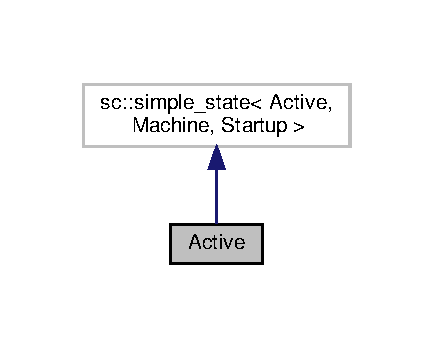
\includegraphics[width=208pt]{structActive__inherit__graph}
\end{center}
\end{figure}


Collaboration diagram for Active\+:
\nopagebreak
\begin{figure}[H]
\begin{center}
\leavevmode
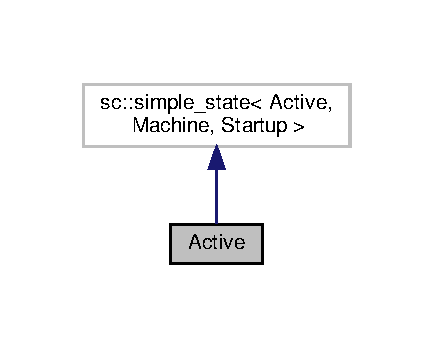
\includegraphics[width=208pt]{structActive__coll__graph}
\end{center}
\end{figure}
\subsection*{Public Member Functions}
\begin{DoxyCompactItemize}
\item 
\mbox{\Hypertarget{structActive_a8a4356547bf4053173248ce72ee076d6}\label{structActive_a8a4356547bf4053173248ce72ee076d6}} 
void {\bfseries set\+Go\+Arm} (const int val)
\end{DoxyCompactItemize}
\subsection*{Public Attributes}
\begin{DoxyCompactItemize}
\item 
\mbox{\Hypertarget{structActive_a4bff8fbeca8d7446793b9349b759c75c}\label{structActive_a4bff8fbeca8d7446793b9349b759c75c}} 
ros\+::\+Publisher {\bfseries gosee\+\_\+pub}
\item 
\mbox{\Hypertarget{structActive_a7ea2eba1cdaa7d6892f1d5b53cf6d972}\label{structActive_a7ea2eba1cdaa7d6892f1d5b53cf6d972}} 
ros\+::\+Publisher {\bfseries gomove\+\_\+pub}
\item 
\mbox{\Hypertarget{structActive_a9ea8f6253991811f556bdec1efe4daee}\label{structActive_a9ea8f6253991811f556bdec1efe4daee}} 
ros\+::\+Publisher {\bfseries table\+\_\+pub}
\item 
\mbox{\Hypertarget{structActive_a22a6505cb6c42d9a6a6dc9ab4d2d568b}\label{structActive_a22a6505cb6c42d9a6a6dc9ab4d2d568b}} 
int {\bfseries go\+\_\+arm}
\end{DoxyCompactItemize}


\subsection{Detailed Description}
structure for \hyperlink{structActive}{Active} state 

The documentation for this struct was generated from the following file\+:\begin{DoxyCompactItemize}
\item 
/home/samuel/\+Desktop/toolcog\+\_\+ws/montecarlo/include/tool\+\_\+expt/\hyperlink{machine_8h}{machine.\+h}\end{DoxyCompactItemize}

\hypertarget{classCreate__Tool}{}\section{Create\+\_\+\+Tool Class Reference}
\label{classCreate__Tool}\index{Create\+\_\+\+Tool@{Create\+\_\+\+Tool}}


Create Tool class object Contains required information for a detect Tool object.  




{\ttfamily \#include $<$create\+\_\+tool.\+h$>$}

\subsection*{Public Member Functions}
\begin{DoxyCompactItemize}
\item 
\mbox{\Hypertarget{classCreate__Tool_a8b1dfbba2c00f29ba9923a68d55bd508}\label{classCreate__Tool_a8b1dfbba2c00f29ba9923a68d55bd508}} 
\hyperlink{classCreate__Tool_a8b1dfbba2c00f29ba9923a68d55bd508}{Create\+\_\+\+Tool} ()
\begin{DoxyCompactList}\small\item\em Construct a new \hyperlink{classCreate__Tool}{Create\+\_\+\+Tool} object. \end{DoxyCompactList}\item 
\mbox{\Hypertarget{classCreate__Tool_af61d80c8faa7752af37806921ddc35e1}\label{classCreate__Tool_af61d80c8faa7752af37806921ddc35e1}} 
\hyperlink{classCreate__Tool_af61d80c8faa7752af37806921ddc35e1}{$\sim$\+Create\+\_\+\+Tool} ()
\begin{DoxyCompactList}\small\item\em Destroy the \hyperlink{classCreate__Tool}{Create\+\_\+\+Tool} object. \end{DoxyCompactList}\item 
\mbox{\Hypertarget{classCreate__Tool_a55627b189b24891751d7101598c6aa0d}\label{classCreate__Tool_a55627b189b24891751d7101598c6aa0d}} 
void \hyperlink{classCreate__Tool_a55627b189b24891751d7101598c6aa0d}{init} ()
\begin{DoxyCompactList}\small\item\em initialise function to set default parameters/stucture objects 1) initialise step size required for monte carlo computation 2) initialise empty tool\+\_\+pose and tool\+\_\+affine 3) initialise a default \textquotesingle{}Tool\textquotesingle{} stucture 4) initialise perception Flag \end{DoxyCompactList}\item 
void \hyperlink{classCreate__Tool_ac8a58a01a4da4d08ae5603e7fee061d6}{create} ()
\begin{DoxyCompactList}\small\item\em function to create 3D Tool object Compute vertices of tested \textquotesingle{}Tool\textquotesingle{} object Fill 3D rotation matrix based on object Generate 3D segment of given object \end{DoxyCompactList}\item 
\mbox{\Hypertarget{classCreate__Tool_acf5f95173cd6baaf110cafb5ff318560}\label{classCreate__Tool_acf5f95173cd6baaf110cafb5ff318560}} 
void \hyperlink{classCreate__Tool_acf5f95173cd6baaf110cafb5ff318560}{display\+Details} (void)
\begin{DoxyCompactList}\small\item\em printing for debug check \end{DoxyCompactList}\item 
vector$<$ Vector3d $>$ \hyperlink{classCreate__Tool_a1393c24c8f96f4e1b41d73db18b720c3}{get\+Vertices} ()
\begin{DoxyCompactList}\small\item\em Get the Vertices object return sets of vertices in 3d coordinates frame. \end{DoxyCompactList}\item 
Vector\+Xd \hyperlink{classCreate__Tool_a0a76e83b7d85e64bb0c9aa8306a0b0f6}{get\+\_\+n\+\_\+pts} ()
\begin{DoxyCompactList}\small\item\em Store the number of point for each segement of each \textquotesingle{}Tool\textquotesingle{} object the number of points in each segment (exclude the edges/extreme\+\_\+pts) \end{DoxyCompactList}\item 
int \hyperlink{classCreate__Tool_a1140f90d5c44110f44939e564646a316}{get\+\_\+\+N\+\_\+seg} ()
\begin{DoxyCompactList}\small\item\em Get the number of segment for this \textquotesingle{}Tool\textquotesingle{} object. \end{DoxyCompactList}\item 
vector$<$ Vector3d $>$ \hyperlink{classCreate__Tool_ac997ba484168b43803bad484f2e4eaaa}{get\+\_\+nvec\+\_\+seg} ()
\begin{DoxyCompactList}\small\item\em Return the normal vector for each segment of this \textquotesingle{}Tool\textquotesingle{} object. \end{DoxyCompactList}\item 
vector$<$ vector$<$ Vector3d $>$ $>$ \hyperlink{classCreate__Tool_a328623ee81b8c11ea9e4dbe8bf863392}{get\+\_\+tool\+\_\+seg} ()
\begin{DoxyCompactList}\small\item\em Get the tool seg object. \end{DoxyCompactList}\item 
Vector\+Xd \hyperlink{classCreate__Tool_a83213666dbbdd99333d84906d1be80e4}{get\+\_\+angle\+\_\+seg} ()
\begin{DoxyCompactList}\small\item\em Get the rotational angles for each segment of the \textquotesingle{}Tool\textquotesingle{} object. \end{DoxyCompactList}\item 
int \hyperlink{classCreate__Tool_a59a084db075fa28aad8251f8c9aee653}{create\+\_\+percept\+Tool} (\hyperlink{structvision__each}{vision\+\_\+each} vdat)
\begin{DoxyCompactList}\small\item\em Create a \textquotesingle{}Tool\textquotesingle{} object from perception data Refer to \hyperlink{vision__data_8h}{vision\+\_\+data.\+h} for perceived object data structure and format. \end{DoxyCompactList}\item 
vector$<$ vector$<$ Vector3d $>$ $>$ \hyperlink{classCreate__Tool_a6e11b0f95ff11d0bd67dade19e17377f}{get\+\_\+seg\+\_\+vertices} ()
\begin{DoxyCompactList}\small\item\em Get every vertices in every segments of this \textquotesingle{}Tool\textquotesingle{} object Each vertice contains the 3d coordinates in (x,y,z) and double data\+\_\+type. \end{DoxyCompactList}\item 
int \hyperlink{classCreate__Tool_a19085ace8b8a30757ba7b5c80cdd0f97}{find\+Grasp\+Loci} ()
\begin{DoxyCompactList}\small\item\em Compute a set of possible grasping location for Olivia to hold. \end{DoxyCompactList}\item 
int \hyperlink{classCreate__Tool_a2dd92335571099de8732d47d7e472865}{write2file} ()
\begin{DoxyCompactList}\small\item\em logging function To record and export all of this \textquotesingle{}Tool\textquotesingle{} object information \end{DoxyCompactList}\end{DoxyCompactItemize}
\subsection*{Public Attributes}
\begin{DoxyCompactItemize}
\item 
\mbox{\Hypertarget{classCreate__Tool_a7302b3e168c45d380194eeed2e863955}\label{classCreate__Tool_a7302b3e168c45d380194eeed2e863955}} 
vector$<$ Affine3d $>$ \hyperlink{classCreate__Tool_a7302b3e168c45d380194eeed2e863955}{grasp\+\_\+loci}
\begin{DoxyCompactList}\small\item\em Store the set of Affine Matrix of possible grasping location in this Tool frame. \end{DoxyCompactList}\end{DoxyCompactItemize}
\subsection*{Private Member Functions}
\begin{DoxyCompactItemize}
\item 
void \hyperlink{classCreate__Tool_a271f74ac5f1fe45a0ee1069f42fbadaf}{fill3\+D\+Rotation} (int idx)
\begin{DoxyCompactList}\small\item\em function to compute and fill the rotational matrix of the selected segment of this \textquotesingle{}Tool\textquotesingle{} object \end{DoxyCompactList}\item 
void \hyperlink{classCreate__Tool_ae2fa728fd141b1eea18ab82cb67c58de}{fill3\+D\+Segment} (int idx)
\begin{DoxyCompactList}\small\item\em function to compute and fill the segmention of the selected segment of this \textquotesingle{}Tool\textquotesingle{} object \end{DoxyCompactList}\item 
double \hyperlink{classCreate__Tool_a7f49a49b557bdde922b2bb7e9c230c6f}{euclidean\+\_\+distance} (Vector3d pt1, Vector3d pt2)
\begin{DoxyCompactList}\small\item\em Function to compute the euclidean\+\_\+distance between 2 points. \end{DoxyCompactList}\item 
std\+::vector$<$ double $>$ \hyperlink{classCreate__Tool_a419350e8721927d095385aa6bef0bc4b}{linspace} (double start\+\_\+in, double end\+\_\+in, int num\+\_\+in)
\begin{DoxyCompactList}\small\item\em Compute linear spacing between a given length. \end{DoxyCompactList}\item 
double \hyperlink{classCreate__Tool_ad015a621844305c141ae1e405402e617}{find\+\_\+angle} (Vector3d pt1, Vector3d pt2, Vector3d pt3)
\begin{DoxyCompactList}\small\item\em compute the angle between 3 given points angle is computed between vector of point12 and point23, join pt1-\/pt2-\/pt3, find angle formed at pt2 between pt1 and pt3. \end{DoxyCompactList}\item 
double \hyperlink{classCreate__Tool_a4a9c9e0219a63df284ece42c198d9c73}{find\+Angle\+Triangle} (Vector3d va, Vector3d vb, Vector3d vc)
\begin{DoxyCompactList}\small\item\em Compute the angle in a triangle formed by 3 vectors assume a triangle and find angle theta at coordinate b (middle argument) a /\textbackslash{} / \textbackslash{} / \textbackslash{} angle@ b /\+\_\+)\+\_\+\+\_\+\+\_\+\+\_\+\textbackslash{} c. \end{DoxyCompactList}\end{DoxyCompactItemize}
\subsection*{Private Attributes}
\begin{DoxyCompactItemize}
\item 
\mbox{\Hypertarget{classCreate__Tool_a2da4141fdf279a34ec7642e02e81ae6f}\label{classCreate__Tool_a2da4141fdf279a34ec7642e02e81ae6f}} 
bool \hyperlink{classCreate__Tool_a2da4141fdf279a34ec7642e02e81ae6f}{percept\+Flag}
\begin{DoxyCompactList}\small\item\em flag to track if this is a default(coded) or a percieved \textquotesingle{}Tool\textquotesingle{} object \end{DoxyCompactList}\item 
\mbox{\Hypertarget{classCreate__Tool_a8751f23989211bc27690cba3aa369e0d}\label{classCreate__Tool_a8751f23989211bc27690cba3aa369e0d}} 
bool \hyperlink{classCreate__Tool_a8751f23989211bc27690cba3aa369e0d}{init\+Flag}
\begin{DoxyCompactList}\small\item\em flag to check if data is properly initialised before computation \end{DoxyCompactList}\item 
\mbox{\Hypertarget{classCreate__Tool_a8d6fff2315a7198c8a59e7c0c48401bd}\label{classCreate__Tool_a8d6fff2315a7198c8a59e7c0c48401bd}} 
int \hyperlink{classCreate__Tool_a8d6fff2315a7198c8a59e7c0c48401bd}{N\+\_\+seg}
\begin{DoxyCompactList}\small\item\em number of segments in this \textquotesingle{}Tool\textquotesingle{} \end{DoxyCompactList}\item 
\mbox{\Hypertarget{classCreate__Tool_aa7dcad369b209d4ee5352e7617762ecf}\label{classCreate__Tool_aa7dcad369b209d4ee5352e7617762ecf}} 
int \hyperlink{classCreate__Tool_aa7dcad369b209d4ee5352e7617762ecf}{prev\+\_\+size}
\begin{DoxyCompactList}\small\item\em store previous size of segment \end{DoxyCompactList}\item 
\mbox{\Hypertarget{classCreate__Tool_a29cf141ff3ce17edd908185bbdb10e8d}\label{classCreate__Tool_a29cf141ff3ce17edd908185bbdb10e8d}} 
double \hyperlink{classCreate__Tool_a29cf141ff3ce17edd908185bbdb10e8d}{len\+\_\+step}
\begin{DoxyCompactList}\small\item\em store step size of each segment (segment length) \end{DoxyCompactList}\item 
\mbox{\Hypertarget{classCreate__Tool_a9f61a626e0c3b4853e0ba7a6834382d2}\label{classCreate__Tool_a9f61a626e0c3b4853e0ba7a6834382d2}} 
double \hyperlink{classCreate__Tool_a9f61a626e0c3b4853e0ba7a6834382d2}{wid\+\_\+seg1}
\begin{DoxyCompactList}\small\item\em store displacement between mesh axis and tool axis \end{DoxyCompactList}\item 
\mbox{\Hypertarget{classCreate__Tool_a8c086a3533361ff6c1614ce3590183f2}\label{classCreate__Tool_a8c086a3533361ff6c1614ce3590183f2}} 
double \hyperlink{classCreate__Tool_a8c086a3533361ff6c1614ce3590183f2}{tool\+\_\+yaw}
\begin{DoxyCompactList}\small\item\em store the yawing(rotation) angle of tool \end{DoxyCompactList}\item 
\mbox{\Hypertarget{classCreate__Tool_add39151bcacd8dec6f1864484f7815be}\label{classCreate__Tool_add39151bcacd8dec6f1864484f7815be}} 
Vector\+Xd \hyperlink{classCreate__Tool_add39151bcacd8dec6f1864484f7815be}{len\+\_\+seg}
\begin{DoxyCompactList}\small\item\em store the length of each segment \end{DoxyCompactList}\item 
\mbox{\Hypertarget{classCreate__Tool_aa76196be75a54a73255131e9ce6b072a}\label{classCreate__Tool_aa76196be75a54a73255131e9ce6b072a}} 
Vector\+Xd \hyperlink{classCreate__Tool_aa76196be75a54a73255131e9ce6b072a}{n\+\_\+pts\+\_\+seg}
\begin{DoxyCompactList}\small\item\em store the number of points in each segment \end{DoxyCompactList}\item 
\mbox{\Hypertarget{classCreate__Tool_a9e73fe1f442a53c41f917cf8937a4216}\label{classCreate__Tool_a9e73fe1f442a53c41f917cf8937a4216}} 
Vector\+Xd \hyperlink{classCreate__Tool_a9e73fe1f442a53c41f917cf8937a4216}{angle\+\_\+seg}
\begin{DoxyCompactList}\small\item\em store the angle of each segment \end{DoxyCompactList}\item 
\mbox{\Hypertarget{classCreate__Tool_ad88f83e484d6945af84f521a2710e4bc}\label{classCreate__Tool_ad88f83e484d6945af84f521a2710e4bc}} 
Vector\+Xd \hyperlink{classCreate__Tool_ad88f83e484d6945af84f521a2710e4bc}{delta\+\_\+angle}
\begin{DoxyCompactList}\small\item\em store the delta (difference) angle for each segment \end{DoxyCompactList}\item 
\mbox{\Hypertarget{classCreate__Tool_aa4242ad29b43cab5ab4d2df4ff44ba9a}\label{classCreate__Tool_aa4242ad29b43cab5ab4d2df4ff44ba9a}} 
int \hyperlink{classCreate__Tool_aa4242ad29b43cab5ab4d2df4ff44ba9a}{prev\+\_\+size\+\_\+2}
\begin{DoxyCompactList}\small\item\em store the previous size of segment \end{DoxyCompactList}\item 
\mbox{\Hypertarget{classCreate__Tool_adaf26bd4949c41ce06895398ab4fa431}\label{classCreate__Tool_adaf26bd4949c41ce06895398ab4fa431}} 
vector$<$ Matrix3d $>$ \hyperlink{classCreate__Tool_adaf26bd4949c41ce06895398ab4fa431}{R3}
\begin{DoxyCompactList}\small\item\em store the rotational matrix for each segment \end{DoxyCompactList}\item 
\mbox{\Hypertarget{classCreate__Tool_a1d9f7d42a254217cb04a7eb599f0fe0c}\label{classCreate__Tool_a1d9f7d42a254217cb04a7eb599f0fe0c}} 
Affine3d \hyperlink{classCreate__Tool_a1d9f7d42a254217cb04a7eb599f0fe0c}{tool\+\_\+affine}
\begin{DoxyCompactList}\small\item\em store the pose of the tool in eigen affine matrix \end{DoxyCompactList}\item 
\mbox{\Hypertarget{classCreate__Tool_a0284095f336cd4847f53a457d1756d1a}\label{classCreate__Tool_a0284095f336cd4847f53a457d1756d1a}} 
Vector3d \hyperlink{classCreate__Tool_a0284095f336cd4847f53a457d1756d1a}{tool\+\_\+trans}
\begin{DoxyCompactList}\small\item\em store the translational vector of the tool \end{DoxyCompactList}\item 
\mbox{\Hypertarget{classCreate__Tool_a086daeeb01921f90e75e49843f6f56e0}\label{classCreate__Tool_a086daeeb01921f90e75e49843f6f56e0}} 
vector$<$ vector$<$ Vector3d $>$ $>$ \hyperlink{classCreate__Tool_a086daeeb01921f90e75e49843f6f56e0}{tool\+\_\+seg\+\_\+3d}
\begin{DoxyCompactList}\small\item\em store the set of vertices that are contained in each segment of the \textquotesingle{}Tool\textquotesingle{} object \end{DoxyCompactList}\item 
\mbox{\Hypertarget{classCreate__Tool_ae753f1f8f15b2e6739e6776642eb4c34}\label{classCreate__Tool_ae753f1f8f15b2e6739e6776642eb4c34}} 
vector$<$ Vector3d $>$ \hyperlink{classCreate__Tool_ae753f1f8f15b2e6739e6776642eb4c34}{nvec\+\_\+seg\+\_\+3d}
\begin{DoxyCompactList}\small\item\em store the normal vector for each segment of the \textquotesingle{}Tool\textquotesingle{} object \end{DoxyCompactList}\item 
\mbox{\Hypertarget{classCreate__Tool_ae02f96935f6b0d5c2a6d76bd421707fc}\label{classCreate__Tool_ae02f96935f6b0d5c2a6d76bd421707fc}} 
vector$<$ Vector3d $>$ \hyperlink{classCreate__Tool_ae02f96935f6b0d5c2a6d76bd421707fc}{tool\+\_\+vertices\+\_\+3d}
\begin{DoxyCompactList}\small\item\em store the 3D vertices of the \textquotesingle{}Tool\textquotesingle{} object \end{DoxyCompactList}\item 
\mbox{\Hypertarget{classCreate__Tool_ae6da0d94feda4e8bb996750d20bf7218}\label{classCreate__Tool_ae6da0d94feda4e8bb996750d20bf7218}} 
vector$<$ float $>$ {\bfseries objheight2table}
\item 
\mbox{\Hypertarget{classCreate__Tool_a86c971fb3705f2d8113118209ca2fba0}\label{classCreate__Tool_a86c971fb3705f2d8113118209ca2fba0}} 
vector$<$ Point\+Cloud$<$ Point\+X\+YZ $>$ $>$ \hyperlink{classCreate__Tool_a86c971fb3705f2d8113118209ca2fba0}{hull\+Clusters\+On\+Axis}
\begin{DoxyCompactList}\small\item\em for each number of \textquotesingle{}Tool\textquotesingle{}, store the 3d coordinates of tool vertices \end{DoxyCompactList}\item 
\mbox{\Hypertarget{classCreate__Tool_abb97ac15169e5df1831b8b8fbf5e4ece}\label{classCreate__Tool_abb97ac15169e5df1831b8b8fbf5e4ece}} 
vector$<$ Matrix4f $>$ \hyperlink{classCreate__Tool_abb97ac15169e5df1831b8b8fbf5e4ece}{proj2\+Table\+T\+Fs}
\begin{DoxyCompactList}\small\item\em for each percieved \textquotesingle{}Tool\textquotesingle{}, store the Transform(\+T\+F) of the tool projection from the table plane \end{DoxyCompactList}\item 
\mbox{\Hypertarget{classCreate__Tool_a3da16d94dd66220185c1adcec47416af}\label{classCreate__Tool_a3da16d94dd66220185c1adcec47416af}} 
vector$<$ vector$<$ Point\+Cloud$<$ Point\+X\+YZ $>$ $>$ $>$ \hyperlink{classCreate__Tool_a3da16d94dd66220185c1adcec47416af}{obj\+\_\+convex}
\begin{DoxyCompactList}\small\item\em for each number of \textquotesingle{}Tool\textquotesingle{}, and for each number of segments in each \textquotesingle{}Tool\textquotesingle{}, store the convex pointcloud points \end{DoxyCompactList}\item 
\mbox{\Hypertarget{classCreate__Tool_a22058ca58e880ab522b8b7872040d175}\label{classCreate__Tool_a22058ca58e880ab522b8b7872040d175}} 
vector$<$ vector$<$ Vector3d $>$ $>$ \hyperlink{classCreate__Tool_a22058ca58e880ab522b8b7872040d175}{seg\+\_\+vertices\+\_\+3d}
\begin{DoxyCompactList}\small\item\em for each number of \textquotesingle{}Tool\textquotesingle{}, and for each number of segments in each \textquotesingle{}Tool\textquotesingle{}, store the 3d coordinates of the vertices \end{DoxyCompactList}\item 
\mbox{\Hypertarget{classCreate__Tool_a6de511d1a128fb0f665c0c70d2caa5f3}\label{classCreate__Tool_a6de511d1a128fb0f665c0c70d2caa5f3}} 
double \hyperlink{classCreate__Tool_a6de511d1a128fb0f665c0c70d2caa5f3}{tool\+\_\+height}
\begin{DoxyCompactList}\small\item\em store the tool height from the table plane \end{DoxyCompactList}\item 
\mbox{\Hypertarget{classCreate__Tool_a59fc2168107cc01207ae6029ddfce8e6}\label{classCreate__Tool_a59fc2168107cc01207ae6029ddfce8e6}} 
int \hyperlink{classCreate__Tool_a59fc2168107cc01207ae6029ddfce8e6}{N\+\_\+pieces}
\begin{DoxyCompactList}\small\item\em how many pieces segmented using P\+CL \end{DoxyCompactList}\end{DoxyCompactItemize}


\subsection{Detailed Description}
Create Tool class object Contains required information for a detect Tool object. 

\subsection{Member Function Documentation}
\mbox{\Hypertarget{classCreate__Tool_ac8a58a01a4da4d08ae5603e7fee061d6}\label{classCreate__Tool_ac8a58a01a4da4d08ae5603e7fee061d6}} 
\index{Create\+\_\+\+Tool@{Create\+\_\+\+Tool}!create@{create}}
\index{create@{create}!Create\+\_\+\+Tool@{Create\+\_\+\+Tool}}
\subsubsection{\texorpdfstring{create()}{create()}}
{\footnotesize\ttfamily void Create\+\_\+\+Tool\+::create (\begin{DoxyParamCaption}{ }\end{DoxyParamCaption})}



function to create 3D Tool object Compute vertices of tested \textquotesingle{}Tool\textquotesingle{} object Fill 3D rotation matrix based on object Generate 3D segment of given object 

W\+H\+EN U\+S\+I\+NG P\+E\+R\+C\+E\+P\+T\+I\+ON M\+O\+D\+U\+LE, U\+SE create\+\_\+percept\+Tool F\+U\+N\+C\+T\+I\+ON instead and provide visual data. \mbox{\Hypertarget{classCreate__Tool_a59a084db075fa28aad8251f8c9aee653}\label{classCreate__Tool_a59a084db075fa28aad8251f8c9aee653}} 
\index{Create\+\_\+\+Tool@{Create\+\_\+\+Tool}!create\+\_\+percept\+Tool@{create\+\_\+percept\+Tool}}
\index{create\+\_\+percept\+Tool@{create\+\_\+percept\+Tool}!Create\+\_\+\+Tool@{Create\+\_\+\+Tool}}
\subsubsection{\texorpdfstring{create\+\_\+percept\+Tool()}{create\_perceptTool()}}
{\footnotesize\ttfamily int Create\+\_\+\+Tool\+::create\+\_\+percept\+Tool (\begin{DoxyParamCaption}\item[{\hyperlink{structvision__each}{vision\+\_\+each}}]{vdat }\end{DoxyParamCaption})}



Create a \textquotesingle{}Tool\textquotesingle{} object from perception data Refer to \hyperlink{vision__data_8h}{vision\+\_\+data.\+h} for perceived object data structure and format. 


\begin{DoxyParams}{Parameters}
{\em vdat} & perception data \\
\hline
\end{DoxyParams}
\begin{DoxyReturn}{Returns}
int 
\end{DoxyReturn}
\mbox{\Hypertarget{classCreate__Tool_a7f49a49b557bdde922b2bb7e9c230c6f}\label{classCreate__Tool_a7f49a49b557bdde922b2bb7e9c230c6f}} 
\index{Create\+\_\+\+Tool@{Create\+\_\+\+Tool}!euclidean\+\_\+distance@{euclidean\+\_\+distance}}
\index{euclidean\+\_\+distance@{euclidean\+\_\+distance}!Create\+\_\+\+Tool@{Create\+\_\+\+Tool}}
\subsubsection{\texorpdfstring{euclidean\+\_\+distance()}{euclidean\_distance()}}
{\footnotesize\ttfamily double Create\+\_\+\+Tool\+::euclidean\+\_\+distance (\begin{DoxyParamCaption}\item[{Vector3d}]{pt1,  }\item[{Vector3d}]{pt2 }\end{DoxyParamCaption})\hspace{0.3cm}{\ttfamily [private]}}



Function to compute the euclidean\+\_\+distance between 2 points. 


\begin{DoxyParams}{Parameters}
{\em pt1} & xyz coordinate of point 1 \\
\hline
{\em pt2} & xyz coordinate of point 2 \\
\hline
\end{DoxyParams}
\begin{DoxyReturn}{Returns}
double distance between points 
\end{DoxyReturn}
\mbox{\Hypertarget{classCreate__Tool_a271f74ac5f1fe45a0ee1069f42fbadaf}\label{classCreate__Tool_a271f74ac5f1fe45a0ee1069f42fbadaf}} 
\index{Create\+\_\+\+Tool@{Create\+\_\+\+Tool}!fill3\+D\+Rotation@{fill3\+D\+Rotation}}
\index{fill3\+D\+Rotation@{fill3\+D\+Rotation}!Create\+\_\+\+Tool@{Create\+\_\+\+Tool}}
\subsubsection{\texorpdfstring{fill3\+D\+Rotation()}{fill3DRotation()}}
{\footnotesize\ttfamily void Create\+\_\+\+Tool\+::fill3\+D\+Rotation (\begin{DoxyParamCaption}\item[{int}]{idx }\end{DoxyParamCaption})\hspace{0.3cm}{\ttfamily [private]}}



function to compute and fill the rotational matrix of the selected segment of this \textquotesingle{}Tool\textquotesingle{} object 


\begin{DoxyParams}{Parameters}
{\em idx} & index of the segment \\
\hline
\end{DoxyParams}
\mbox{\Hypertarget{classCreate__Tool_ae2fa728fd141b1eea18ab82cb67c58de}\label{classCreate__Tool_ae2fa728fd141b1eea18ab82cb67c58de}} 
\index{Create\+\_\+\+Tool@{Create\+\_\+\+Tool}!fill3\+D\+Segment@{fill3\+D\+Segment}}
\index{fill3\+D\+Segment@{fill3\+D\+Segment}!Create\+\_\+\+Tool@{Create\+\_\+\+Tool}}
\subsubsection{\texorpdfstring{fill3\+D\+Segment()}{fill3DSegment()}}
{\footnotesize\ttfamily void Create\+\_\+\+Tool\+::fill3\+D\+Segment (\begin{DoxyParamCaption}\item[{int}]{idx }\end{DoxyParamCaption})\hspace{0.3cm}{\ttfamily [private]}}



function to compute and fill the segmention of the selected segment of this \textquotesingle{}Tool\textquotesingle{} object 


\begin{DoxyParams}{Parameters}
{\em idx} & index of the segment \\
\hline
\end{DoxyParams}
\mbox{\Hypertarget{classCreate__Tool_ad015a621844305c141ae1e405402e617}\label{classCreate__Tool_ad015a621844305c141ae1e405402e617}} 
\index{Create\+\_\+\+Tool@{Create\+\_\+\+Tool}!find\+\_\+angle@{find\+\_\+angle}}
\index{find\+\_\+angle@{find\+\_\+angle}!Create\+\_\+\+Tool@{Create\+\_\+\+Tool}}
\subsubsection{\texorpdfstring{find\+\_\+angle()}{find\_angle()}}
{\footnotesize\ttfamily double Create\+\_\+\+Tool\+::find\+\_\+angle (\begin{DoxyParamCaption}\item[{Vector3d}]{pt1,  }\item[{Vector3d}]{pt2,  }\item[{Vector3d}]{pt3 }\end{DoxyParamCaption})\hspace{0.3cm}{\ttfamily [private]}}



compute the angle between 3 given points angle is computed between vector of point12 and point23, join pt1-\/pt2-\/pt3, find angle formed at pt2 between pt1 and pt3. 


\begin{DoxyParams}{Parameters}
{\em pt1} & point 1 \\
\hline
{\em pt2} & point 2 \\
\hline
{\em pt3} & point 3 \\
\hline
\end{DoxyParams}
\begin{DoxyReturn}{Returns}
double angle in radian 
\end{DoxyReturn}
\mbox{\Hypertarget{classCreate__Tool_a4a9c9e0219a63df284ece42c198d9c73}\label{classCreate__Tool_a4a9c9e0219a63df284ece42c198d9c73}} 
\index{Create\+\_\+\+Tool@{Create\+\_\+\+Tool}!find\+Angle\+Triangle@{find\+Angle\+Triangle}}
\index{find\+Angle\+Triangle@{find\+Angle\+Triangle}!Create\+\_\+\+Tool@{Create\+\_\+\+Tool}}
\subsubsection{\texorpdfstring{find\+Angle\+Triangle()}{findAngleTriangle()}}
{\footnotesize\ttfamily double Create\+\_\+\+Tool\+::find\+Angle\+Triangle (\begin{DoxyParamCaption}\item[{Vector3d}]{va,  }\item[{Vector3d}]{vb,  }\item[{Vector3d}]{vc }\end{DoxyParamCaption})\hspace{0.3cm}{\ttfamily [private]}}



Compute the angle in a triangle formed by 3 vectors assume a triangle and find angle theta at coordinate b (middle argument) a /\textbackslash{} / \textbackslash{} / \textbackslash{} angle@ b /\+\_\+)\+\_\+\+\_\+\+\_\+\+\_\+\textbackslash{} c. 


\begin{DoxyParams}{Parameters}
{\em va} & vector 1 \\
\hline
{\em vb} & vector 2 \\
\hline
{\em vc} & vector 3 \\
\hline
\end{DoxyParams}
\begin{DoxyReturn}{Returns}
double angle in radian 
\end{DoxyReturn}
\mbox{\Hypertarget{classCreate__Tool_a19085ace8b8a30757ba7b5c80cdd0f97}\label{classCreate__Tool_a19085ace8b8a30757ba7b5c80cdd0f97}} 
\index{Create\+\_\+\+Tool@{Create\+\_\+\+Tool}!find\+Grasp\+Loci@{find\+Grasp\+Loci}}
\index{find\+Grasp\+Loci@{find\+Grasp\+Loci}!Create\+\_\+\+Tool@{Create\+\_\+\+Tool}}
\subsubsection{\texorpdfstring{find\+Grasp\+Loci()}{findGraspLoci()}}
{\footnotesize\ttfamily int Create\+\_\+\+Tool\+::find\+Grasp\+Loci (\begin{DoxyParamCaption}{ }\end{DoxyParamCaption})}



Compute a set of possible grasping location for Olivia to hold. 

\begin{DoxyReturn}{Returns}
int 
\end{DoxyReturn}
\mbox{\Hypertarget{classCreate__Tool_a83213666dbbdd99333d84906d1be80e4}\label{classCreate__Tool_a83213666dbbdd99333d84906d1be80e4}} 
\index{Create\+\_\+\+Tool@{Create\+\_\+\+Tool}!get\+\_\+angle\+\_\+seg@{get\+\_\+angle\+\_\+seg}}
\index{get\+\_\+angle\+\_\+seg@{get\+\_\+angle\+\_\+seg}!Create\+\_\+\+Tool@{Create\+\_\+\+Tool}}
\subsubsection{\texorpdfstring{get\+\_\+angle\+\_\+seg()}{get\_angle\_seg()}}
{\footnotesize\ttfamily Vector\+Xd Create\+\_\+\+Tool\+::get\+\_\+angle\+\_\+seg (\begin{DoxyParamCaption}{ }\end{DoxyParamCaption})\hspace{0.3cm}{\ttfamily [inline]}}



Get the rotational angles for each segment of the \textquotesingle{}Tool\textquotesingle{} object. 

\begin{DoxyReturn}{Returns}
Vector\+Xd 
\end{DoxyReturn}
\mbox{\Hypertarget{classCreate__Tool_a0a76e83b7d85e64bb0c9aa8306a0b0f6}\label{classCreate__Tool_a0a76e83b7d85e64bb0c9aa8306a0b0f6}} 
\index{Create\+\_\+\+Tool@{Create\+\_\+\+Tool}!get\+\_\+n\+\_\+pts@{get\+\_\+n\+\_\+pts}}
\index{get\+\_\+n\+\_\+pts@{get\+\_\+n\+\_\+pts}!Create\+\_\+\+Tool@{Create\+\_\+\+Tool}}
\subsubsection{\texorpdfstring{get\+\_\+n\+\_\+pts()}{get\_n\_pts()}}
{\footnotesize\ttfamily Vector\+Xd Create\+\_\+\+Tool\+::get\+\_\+n\+\_\+pts (\begin{DoxyParamCaption}{ }\end{DoxyParamCaption})}



Store the number of point for each segement of each \textquotesingle{}Tool\textquotesingle{} object the number of points in each segment (exclude the edges/extreme\+\_\+pts) 

\begin{DoxyReturn}{Returns}
Vector\+Xd 
\end{DoxyReturn}
\mbox{\Hypertarget{classCreate__Tool_a1140f90d5c44110f44939e564646a316}\label{classCreate__Tool_a1140f90d5c44110f44939e564646a316}} 
\index{Create\+\_\+\+Tool@{Create\+\_\+\+Tool}!get\+\_\+\+N\+\_\+seg@{get\+\_\+\+N\+\_\+seg}}
\index{get\+\_\+\+N\+\_\+seg@{get\+\_\+\+N\+\_\+seg}!Create\+\_\+\+Tool@{Create\+\_\+\+Tool}}
\subsubsection{\texorpdfstring{get\+\_\+\+N\+\_\+seg()}{get\_N\_seg()}}
{\footnotesize\ttfamily int Create\+\_\+\+Tool\+::get\+\_\+\+N\+\_\+seg (\begin{DoxyParamCaption}{ }\end{DoxyParamCaption})\hspace{0.3cm}{\ttfamily [inline]}}



Get the number of segment for this \textquotesingle{}Tool\textquotesingle{} object. 

\begin{DoxyReturn}{Returns}
int number of segments 
\end{DoxyReturn}
\mbox{\Hypertarget{classCreate__Tool_ac997ba484168b43803bad484f2e4eaaa}\label{classCreate__Tool_ac997ba484168b43803bad484f2e4eaaa}} 
\index{Create\+\_\+\+Tool@{Create\+\_\+\+Tool}!get\+\_\+nvec\+\_\+seg@{get\+\_\+nvec\+\_\+seg}}
\index{get\+\_\+nvec\+\_\+seg@{get\+\_\+nvec\+\_\+seg}!Create\+\_\+\+Tool@{Create\+\_\+\+Tool}}
\subsubsection{\texorpdfstring{get\+\_\+nvec\+\_\+seg()}{get\_nvec\_seg()}}
{\footnotesize\ttfamily vector$<$ Vector3d $>$ Create\+\_\+\+Tool\+::get\+\_\+nvec\+\_\+seg (\begin{DoxyParamCaption}{ }\end{DoxyParamCaption})\hspace{0.3cm}{\ttfamily [inline]}}



Return the normal vector for each segment of this \textquotesingle{}Tool\textquotesingle{} object. 

\begin{DoxyReturn}{Returns}
vector$<$ Vector3d $>$ sets of normal\+\_\+vector for each segment 
\end{DoxyReturn}
\mbox{\Hypertarget{classCreate__Tool_a6e11b0f95ff11d0bd67dade19e17377f}\label{classCreate__Tool_a6e11b0f95ff11d0bd67dade19e17377f}} 
\index{Create\+\_\+\+Tool@{Create\+\_\+\+Tool}!get\+\_\+seg\+\_\+vertices@{get\+\_\+seg\+\_\+vertices}}
\index{get\+\_\+seg\+\_\+vertices@{get\+\_\+seg\+\_\+vertices}!Create\+\_\+\+Tool@{Create\+\_\+\+Tool}}
\subsubsection{\texorpdfstring{get\+\_\+seg\+\_\+vertices()}{get\_seg\_vertices()}}
{\footnotesize\ttfamily vector$<$ vector$<$Vector3d$>$ $>$ Create\+\_\+\+Tool\+::get\+\_\+seg\+\_\+vertices (\begin{DoxyParamCaption}{ }\end{DoxyParamCaption})\hspace{0.3cm}{\ttfamily [inline]}}



Get every vertices in every segments of this \textquotesingle{}Tool\textquotesingle{} object Each vertice contains the 3d coordinates in (x,y,z) and double data\+\_\+type. 

\begin{DoxyReturn}{Returns}
vector$<$ vector$<$\+Vector3d$>$ $>$ 3d sets of verticles in every segment of this tool 
\end{DoxyReturn}
\mbox{\Hypertarget{classCreate__Tool_a328623ee81b8c11ea9e4dbe8bf863392}\label{classCreate__Tool_a328623ee81b8c11ea9e4dbe8bf863392}} 
\index{Create\+\_\+\+Tool@{Create\+\_\+\+Tool}!get\+\_\+tool\+\_\+seg@{get\+\_\+tool\+\_\+seg}}
\index{get\+\_\+tool\+\_\+seg@{get\+\_\+tool\+\_\+seg}!Create\+\_\+\+Tool@{Create\+\_\+\+Tool}}
\subsubsection{\texorpdfstring{get\+\_\+tool\+\_\+seg()}{get\_tool\_seg()}}
{\footnotesize\ttfamily vector$<$ vector$<$Vector3d$>$ $>$ Create\+\_\+\+Tool\+::get\+\_\+tool\+\_\+seg (\begin{DoxyParamCaption}{ }\end{DoxyParamCaption})\hspace{0.3cm}{\ttfamily [inline]}}



Get the tool seg object. 

\begin{DoxyReturn}{Returns}
vector$<$ vector$<$\+Vector3d$>$ $>$ 3d coordinates for each point in each segment 
\end{DoxyReturn}
\mbox{\Hypertarget{classCreate__Tool_a1393c24c8f96f4e1b41d73db18b720c3}\label{classCreate__Tool_a1393c24c8f96f4e1b41d73db18b720c3}} 
\index{Create\+\_\+\+Tool@{Create\+\_\+\+Tool}!get\+Vertices@{get\+Vertices}}
\index{get\+Vertices@{get\+Vertices}!Create\+\_\+\+Tool@{Create\+\_\+\+Tool}}
\subsubsection{\texorpdfstring{get\+Vertices()}{getVertices()}}
{\footnotesize\ttfamily vector$<$ Vector3d $>$ Create\+\_\+\+Tool\+::get\+Vertices (\begin{DoxyParamCaption}{ }\end{DoxyParamCaption})\hspace{0.3cm}{\ttfamily [inline]}}



Get the Vertices object return sets of vertices in 3d coordinates frame. 

\begin{DoxyReturn}{Returns}
vector$<$ Vector3d $>$ sets of verticles from created \textquotesingle{}Tool\textquotesingle{} object 
\end{DoxyReturn}
\mbox{\Hypertarget{classCreate__Tool_a419350e8721927d095385aa6bef0bc4b}\label{classCreate__Tool_a419350e8721927d095385aa6bef0bc4b}} 
\index{Create\+\_\+\+Tool@{Create\+\_\+\+Tool}!linspace@{linspace}}
\index{linspace@{linspace}!Create\+\_\+\+Tool@{Create\+\_\+\+Tool}}
\subsubsection{\texorpdfstring{linspace()}{linspace()}}
{\footnotesize\ttfamily std\+::vector$<$ double $>$ Create\+\_\+\+Tool\+::linspace (\begin{DoxyParamCaption}\item[{double}]{start\+\_\+in,  }\item[{double}]{end\+\_\+in,  }\item[{int}]{num\+\_\+in }\end{DoxyParamCaption})\hspace{0.3cm}{\ttfamily [private]}}



Compute linear spacing between a given length. 


\begin{DoxyParams}{Parameters}
{\em start\+\_\+in} & start coordinate \\
\hline
{\em end\+\_\+in} & end coordinate \\
\hline
{\em num\+\_\+in} & number of spacing \\
\hline
\end{DoxyParams}
\begin{DoxyReturn}{Returns}
std\+::vector$<$double$>$ vector containing the coordinate of each spacing 
\end{DoxyReturn}
\mbox{\Hypertarget{classCreate__Tool_a2dd92335571099de8732d47d7e472865}\label{classCreate__Tool_a2dd92335571099de8732d47d7e472865}} 
\index{Create\+\_\+\+Tool@{Create\+\_\+\+Tool}!write2file@{write2file}}
\index{write2file@{write2file}!Create\+\_\+\+Tool@{Create\+\_\+\+Tool}}
\subsubsection{\texorpdfstring{write2file()}{write2file()}}
{\footnotesize\ttfamily int Create\+\_\+\+Tool\+::write2file (\begin{DoxyParamCaption}{ }\end{DoxyParamCaption})}



logging function To record and export all of this \textquotesingle{}Tool\textquotesingle{} object information 

\begin{DoxyReturn}{Returns}
int 
\end{DoxyReturn}


The documentation for this class was generated from the following files\+:\begin{DoxyCompactItemize}
\item 
/home/samuel/\+Desktop/toolcog\+\_\+ws/montecarlo/include/tool\+\_\+expt/\hyperlink{create__tool_8h}{create\+\_\+tool.\+h}\item 
/home/samuel/\+Desktop/toolcog\+\_\+ws/montecarlo/src/create\+\_\+tool.\+cpp\end{DoxyCompactItemize}

\hypertarget{structdataset}{}\section{dataset Struct Reference}
\label{structdataset}\index{dataset@{dataset}}


structure for data to record. Add more data entry here.  




{\ttfamily \#include $<$recorder.\+h$>$}

\subsection*{Public Attributes}
\begin{DoxyCompactItemize}
\item 
\mbox{\Hypertarget{structdataset_a18ad09e1e8d828bb47c9c97ba8fb19ff}\label{structdataset_a18ad09e1e8d828bb47c9c97ba8fb19ff}} 
int {\bfseries col\+Flag}
\item 
\mbox{\Hypertarget{structdataset_a538895328f6fdcdf1961886b9b87ef4a}\label{structdataset_a538895328f6fdcdf1961886b9b87ef4a}} 
int {\bfseries small\+Flag}
\item 
\mbox{\Hypertarget{structdataset_a99b024d8545e437d501de41972cc7f78}\label{structdataset_a99b024d8545e437d501de41972cc7f78}} 
double {\bfseries score}
\item 
\mbox{\Hypertarget{structdataset_adb82f6ebc39f6b4bcd76da5b4351d459}\label{structdataset_adb82f6ebc39f6b4bcd76da5b4351d459}} 
int {\bfseries num\+\_\+visit}
\item 
\mbox{\Hypertarget{structdataset_a2b08b466539366cbeac52c06e282bb13}\label{structdataset_a2b08b466539366cbeac52c06e282bb13}} 
int {\bfseries index} \mbox{[}7\mbox{]}
\item 
\mbox{\Hypertarget{structdataset_a8fc49f276f433cc35ca1444154ea7bad}\label{structdataset_a8fc49f276f433cc35ca1444154ea7bad}} 
string {\bfseries label}
\item 
\mbox{\Hypertarget{structdataset_a288f4d9ae8fdb1df154d5766cf6d878c}\label{structdataset_a288f4d9ae8fdb1df154d5766cf6d878c}} 
string {\bfseries type}
\end{DoxyCompactItemize}


\subsection{Detailed Description}
structure for data to record. Add more data entry here. 

The documentation for this struct was generated from the following file\+:\begin{DoxyCompactItemize}
\item 
/home/samuel/\+Desktop/toolcog\+\_\+ws/montecarlo/include/tool\+\_\+expt/\hyperlink{recorder_8h}{recorder.\+h}\end{DoxyCompactItemize}

\hypertarget{structEvMonteCarloExpt}{}\section{Ev\+Monte\+Carlo\+Expt Struct Reference}
\label{structEvMonteCarloExpt}\index{Ev\+Monte\+Carlo\+Expt@{Ev\+Monte\+Carlo\+Expt}}


State machine Event structure\+: Monte Carlo search experiment.  




{\ttfamily \#include $<$machine.\+h$>$}



Inheritance diagram for Ev\+Monte\+Carlo\+Expt\+:
\nopagebreak
\begin{figure}[H]
\begin{center}
\leavevmode
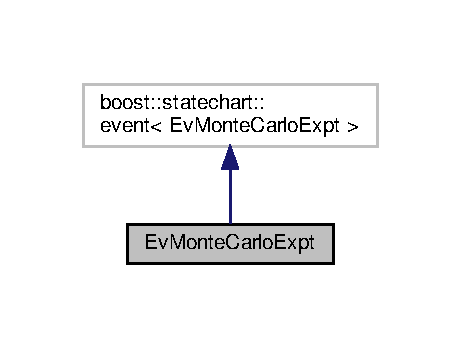
\includegraphics[width=221pt]{structEvMonteCarloExpt__inherit__graph}
\end{center}
\end{figure}


Collaboration diagram for Ev\+Monte\+Carlo\+Expt\+:
\nopagebreak
\begin{figure}[H]
\begin{center}
\leavevmode
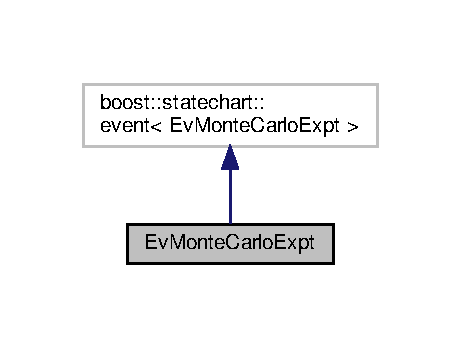
\includegraphics[width=221pt]{structEvMonteCarloExpt__coll__graph}
\end{center}
\end{figure}


\subsection{Detailed Description}
State machine Event structure\+: Monte Carlo search experiment. 

The documentation for this struct was generated from the following file\+:\begin{DoxyCompactItemize}
\item 
/home/samuel/\+Desktop/toolcog\+\_\+ws/montecarlo/include/tool\+\_\+expt/\hyperlink{machine_8h}{machine.\+h}\end{DoxyCompactItemize}

\hypertarget{structEvMonteCarloExpt2}{}\section{Ev\+Monte\+Carlo\+Expt2 Struct Reference}
\label{structEvMonteCarloExpt2}\index{Ev\+Monte\+Carlo\+Expt2@{Ev\+Monte\+Carlo\+Expt2}}


State machine Event structure\+: Monte Carlo search experiment 2.  




{\ttfamily \#include $<$machine.\+h$>$}



Inheritance diagram for Ev\+Monte\+Carlo\+Expt2\+:
\nopagebreak
\begin{figure}[H]
\begin{center}
\leavevmode
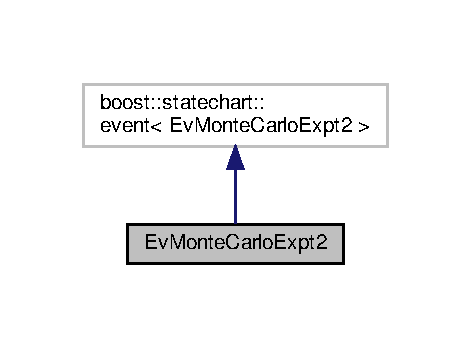
\includegraphics[width=226pt]{structEvMonteCarloExpt2__inherit__graph}
\end{center}
\end{figure}


Collaboration diagram for Ev\+Monte\+Carlo\+Expt2\+:
\nopagebreak
\begin{figure}[H]
\begin{center}
\leavevmode
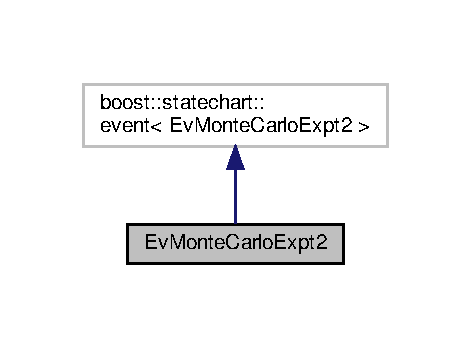
\includegraphics[width=226pt]{structEvMonteCarloExpt2__coll__graph}
\end{center}
\end{figure}


\subsection{Detailed Description}
State machine Event structure\+: Monte Carlo search experiment 2. 

The documentation for this struct was generated from the following file\+:\begin{DoxyCompactItemize}
\item 
/home/samuel/\+Desktop/toolcog\+\_\+ws/montecarlo/include/tool\+\_\+expt/\hyperlink{machine_8h}{machine.\+h}\end{DoxyCompactItemize}

\hypertarget{structEvMonteCarloExpt2__left}{}\section{Ev\+Monte\+Carlo\+Expt2\+\_\+left Struct Reference}
\label{structEvMonteCarloExpt2__left}\index{Ev\+Monte\+Carlo\+Expt2\+\_\+left@{Ev\+Monte\+Carlo\+Expt2\+\_\+left}}


State machine Event structure\+: Monte Carlo search experiment 2 with Left Arm of Olivia.  




{\ttfamily \#include $<$machine.\+h$>$}



Inheritance diagram for Ev\+Monte\+Carlo\+Expt2\+\_\+left\+:
\nopagebreak
\begin{figure}[H]
\begin{center}
\leavevmode
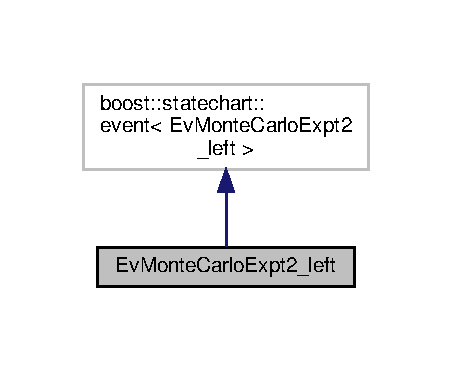
\includegraphics[width=217pt]{structEvMonteCarloExpt2__left__inherit__graph}
\end{center}
\end{figure}


Collaboration diagram for Ev\+Monte\+Carlo\+Expt2\+\_\+left\+:
\nopagebreak
\begin{figure}[H]
\begin{center}
\leavevmode
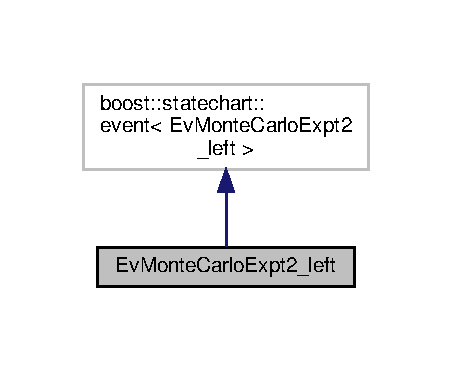
\includegraphics[width=217pt]{structEvMonteCarloExpt2__left__coll__graph}
\end{center}
\end{figure}


\subsection{Detailed Description}
State machine Event structure\+: Monte Carlo search experiment 2 with Left Arm of Olivia. 

The documentation for this struct was generated from the following file\+:\begin{DoxyCompactItemize}
\item 
/home/samuel/\+Desktop/toolcog\+\_\+ws/montecarlo/include/tool\+\_\+expt/\hyperlink{machine_8h}{machine.\+h}\end{DoxyCompactItemize}

\hypertarget{structEvMonteCarloExpt3__left}{}\section{Ev\+Monte\+Carlo\+Expt3\+\_\+left Struct Reference}
\label{structEvMonteCarloExpt3__left}\index{Ev\+Monte\+Carlo\+Expt3\+\_\+left@{Ev\+Monte\+Carlo\+Expt3\+\_\+left}}


State machine Event structure\+: Monte Carlo search experiment 3 with Left Arm of Olivia.  




{\ttfamily \#include $<$machine.\+h$>$}



Inheritance diagram for Ev\+Monte\+Carlo\+Expt3\+\_\+left\+:
\nopagebreak
\begin{figure}[H]
\begin{center}
\leavevmode
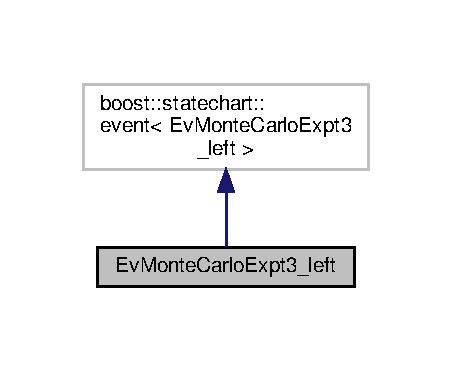
\includegraphics[width=217pt]{structEvMonteCarloExpt3__left__inherit__graph}
\end{center}
\end{figure}


Collaboration diagram for Ev\+Monte\+Carlo\+Expt3\+\_\+left\+:
\nopagebreak
\begin{figure}[H]
\begin{center}
\leavevmode
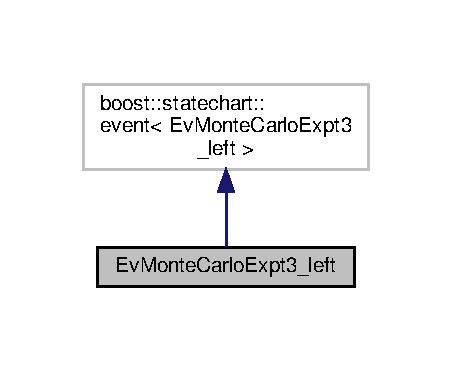
\includegraphics[width=217pt]{structEvMonteCarloExpt3__left__coll__graph}
\end{center}
\end{figure}


\subsection{Detailed Description}
State machine Event structure\+: Monte Carlo search experiment 3 with Left Arm of Olivia. 

The documentation for this struct was generated from the following file\+:\begin{DoxyCompactItemize}
\item 
/home/samuel/\+Desktop/toolcog\+\_\+ws/montecarlo/include/tool\+\_\+expt/\hyperlink{machine_8h}{machine.\+h}\end{DoxyCompactItemize}

\hypertarget{structEvObjectBackOfTargetRightOfRobot}{}\section{Ev\+Object\+Back\+Of\+Target\+Right\+Of\+Robot Struct Reference}
\label{structEvObjectBackOfTargetRightOfRobot}\index{Ev\+Object\+Back\+Of\+Target\+Right\+Of\+Robot@{Ev\+Object\+Back\+Of\+Target\+Right\+Of\+Robot}}


State machine Event structure\+: Right Body Sequence when object is behind target goal.  




{\ttfamily \#include $<$machine.\+h$>$}



Inheritance diagram for Ev\+Object\+Back\+Of\+Target\+Right\+Of\+Robot\+:
\nopagebreak
\begin{figure}[H]
\begin{center}
\leavevmode
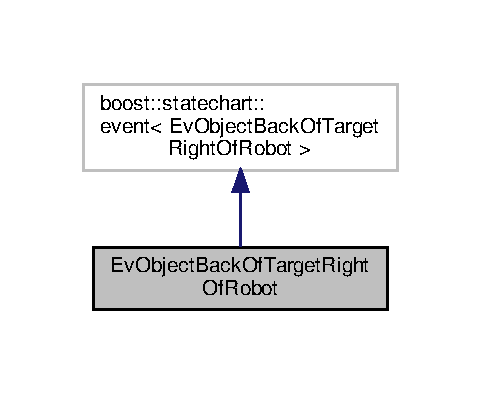
\includegraphics[width=231pt]{structEvObjectBackOfTargetRightOfRobot__inherit__graph}
\end{center}
\end{figure}


Collaboration diagram for Ev\+Object\+Back\+Of\+Target\+Right\+Of\+Robot\+:
\nopagebreak
\begin{figure}[H]
\begin{center}
\leavevmode
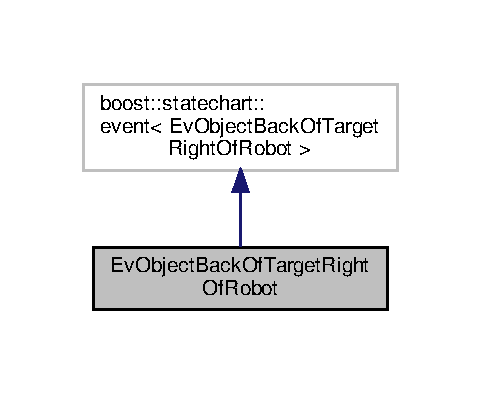
\includegraphics[width=231pt]{structEvObjectBackOfTargetRightOfRobot__coll__graph}
\end{center}
\end{figure}


\subsection{Detailed Description}
State machine Event structure\+: Right Body Sequence when object is behind target goal. 

The documentation for this struct was generated from the following file\+:\begin{DoxyCompactItemize}
\item 
/home/samuel/\+Desktop/toolcog\+\_\+ws/montecarlo/include/tool\+\_\+expt/\hyperlink{machine_8h}{machine.\+h}\end{DoxyCompactItemize}

\hypertarget{structEvObjectBackOfTargetRightOfRobotTool}{}\section{Ev\+Object\+Back\+Of\+Target\+Right\+Of\+Robot\+Tool Struct Reference}
\label{structEvObjectBackOfTargetRightOfRobotTool}\index{Ev\+Object\+Back\+Of\+Target\+Right\+Of\+Robot\+Tool@{Ev\+Object\+Back\+Of\+Target\+Right\+Of\+Robot\+Tool}}


State machine Event structure\+: Sequence when object is behind and right of tool.  




{\ttfamily \#include $<$machine.\+h$>$}



Inheritance diagram for Ev\+Object\+Back\+Of\+Target\+Right\+Of\+Robot\+Tool\+:
\nopagebreak
\begin{figure}[H]
\begin{center}
\leavevmode
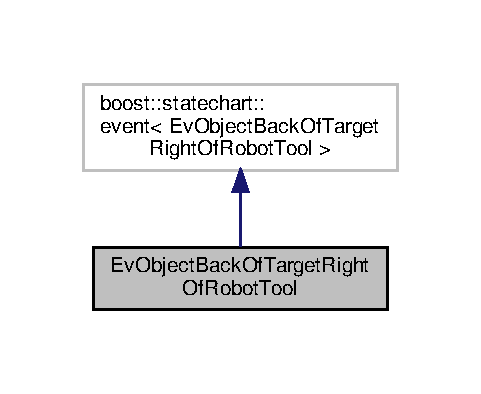
\includegraphics[width=231pt]{structEvObjectBackOfTargetRightOfRobotTool__inherit__graph}
\end{center}
\end{figure}


Collaboration diagram for Ev\+Object\+Back\+Of\+Target\+Right\+Of\+Robot\+Tool\+:
\nopagebreak
\begin{figure}[H]
\begin{center}
\leavevmode
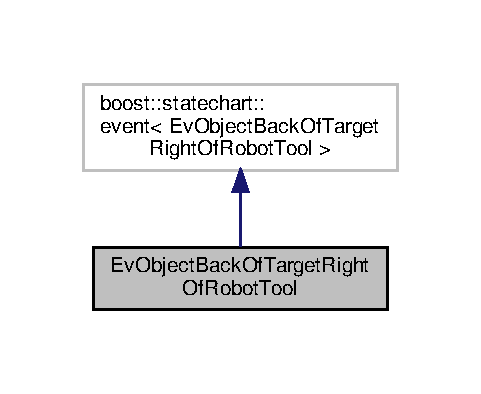
\includegraphics[width=231pt]{structEvObjectBackOfTargetRightOfRobotTool__coll__graph}
\end{center}
\end{figure}


\subsection{Detailed Description}
State machine Event structure\+: Sequence when object is behind and right of tool. 

The documentation for this struct was generated from the following file\+:\begin{DoxyCompactItemize}
\item 
/home/samuel/\+Desktop/toolcog\+\_\+ws/montecarlo/include/tool\+\_\+expt/\hyperlink{machine_8h}{machine.\+h}\end{DoxyCompactItemize}

\hypertarget{structEvObjectBackRightOfTargetTool}{}\section{Ev\+Object\+Back\+Right\+Of\+Target\+Tool Struct Reference}
\label{structEvObjectBackRightOfTargetTool}\index{Ev\+Object\+Back\+Right\+Of\+Target\+Tool@{Ev\+Object\+Back\+Right\+Of\+Target\+Tool}}


State machine Event structure\+: Sequence when object is on back right of tool.  




{\ttfamily \#include $<$machine.\+h$>$}



Inheritance diagram for Ev\+Object\+Back\+Right\+Of\+Target\+Tool\+:
\nopagebreak
\begin{figure}[H]
\begin{center}
\leavevmode
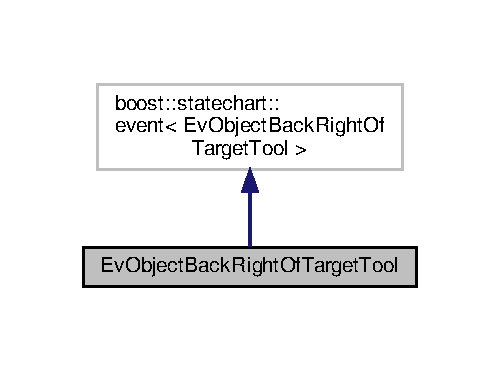
\includegraphics[width=240pt]{structEvObjectBackRightOfTargetTool__inherit__graph}
\end{center}
\end{figure}


Collaboration diagram for Ev\+Object\+Back\+Right\+Of\+Target\+Tool\+:
\nopagebreak
\begin{figure}[H]
\begin{center}
\leavevmode
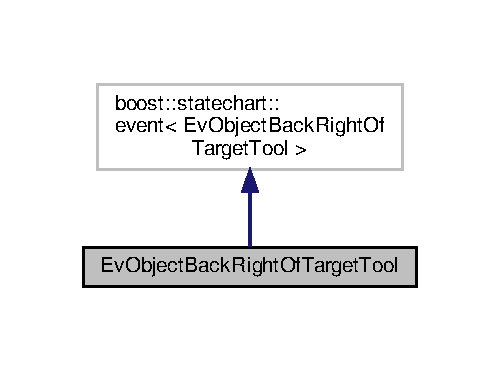
\includegraphics[width=240pt]{structEvObjectBackRightOfTargetTool__coll__graph}
\end{center}
\end{figure}


\subsection{Detailed Description}
State machine Event structure\+: Sequence when object is on back right of tool. 

The documentation for this struct was generated from the following file\+:\begin{DoxyCompactItemize}
\item 
/home/samuel/\+Desktop/toolcog\+\_\+ws/montecarlo/include/tool\+\_\+expt/\hyperlink{machine_8h}{machine.\+h}\end{DoxyCompactItemize}

\hypertarget{structEvObjectFrontOfTargetLeftOfRobotTool}{}\section{Ev\+Object\+Front\+Of\+Target\+Left\+Of\+Robot\+Tool Struct Reference}
\label{structEvObjectFrontOfTargetLeftOfRobotTool}\index{Ev\+Object\+Front\+Of\+Target\+Left\+Of\+Robot\+Tool@{Ev\+Object\+Front\+Of\+Target\+Left\+Of\+Robot\+Tool}}


State machine Event structure\+: Sequence when object is on the front left of tool.  




{\ttfamily \#include $<$machine.\+h$>$}



Inheritance diagram for Ev\+Object\+Front\+Of\+Target\+Left\+Of\+Robot\+Tool\+:
\nopagebreak
\begin{figure}[H]
\begin{center}
\leavevmode
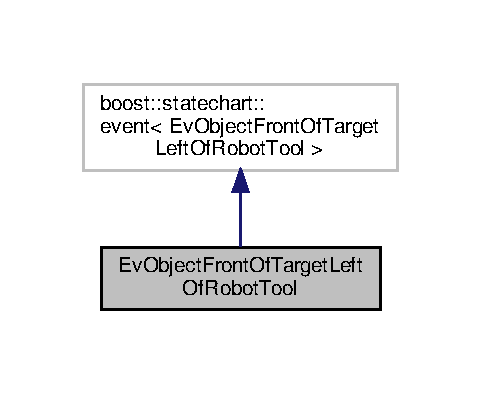
\includegraphics[width=231pt]{structEvObjectFrontOfTargetLeftOfRobotTool__inherit__graph}
\end{center}
\end{figure}


Collaboration diagram for Ev\+Object\+Front\+Of\+Target\+Left\+Of\+Robot\+Tool\+:
\nopagebreak
\begin{figure}[H]
\begin{center}
\leavevmode
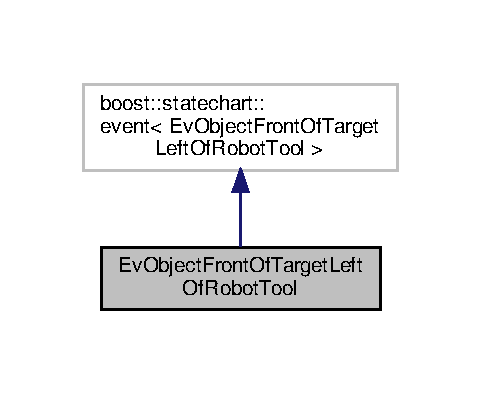
\includegraphics[width=231pt]{structEvObjectFrontOfTargetLeftOfRobotTool__coll__graph}
\end{center}
\end{figure}


\subsection{Detailed Description}
State machine Event structure\+: Sequence when object is on the front left of tool. 

The documentation for this struct was generated from the following file\+:\begin{DoxyCompactItemize}
\item 
/home/samuel/\+Desktop/toolcog\+\_\+ws/montecarlo/include/tool\+\_\+expt/\hyperlink{machine_8h}{machine.\+h}\end{DoxyCompactItemize}

\hypertarget{structEvObjectFrontOfTargetRightOfRobot}{}\section{Ev\+Object\+Front\+Of\+Target\+Right\+Of\+Robot Struct Reference}
\label{structEvObjectFrontOfTargetRightOfRobot}\index{Ev\+Object\+Front\+Of\+Target\+Right\+Of\+Robot@{Ev\+Object\+Front\+Of\+Target\+Right\+Of\+Robot}}


State machine Event structure\+: Right Body Sequence when object in front of target goal.  




{\ttfamily \#include $<$machine.\+h$>$}



Inheritance diagram for Ev\+Object\+Front\+Of\+Target\+Right\+Of\+Robot\+:
\nopagebreak
\begin{figure}[H]
\begin{center}
\leavevmode
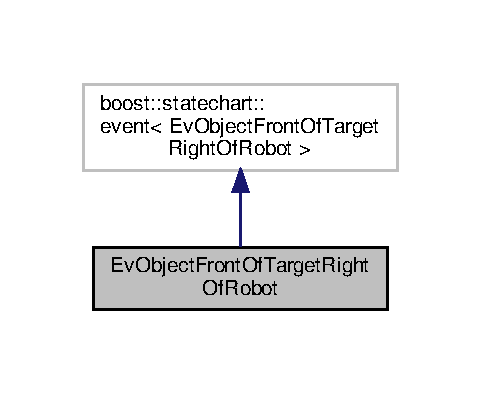
\includegraphics[width=231pt]{structEvObjectFrontOfTargetRightOfRobot__inherit__graph}
\end{center}
\end{figure}


Collaboration diagram for Ev\+Object\+Front\+Of\+Target\+Right\+Of\+Robot\+:
\nopagebreak
\begin{figure}[H]
\begin{center}
\leavevmode
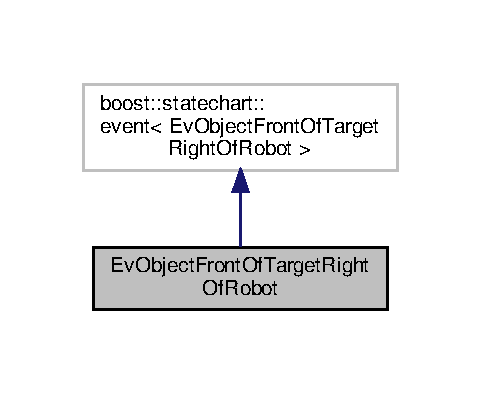
\includegraphics[width=231pt]{structEvObjectFrontOfTargetRightOfRobot__coll__graph}
\end{center}
\end{figure}


\subsection{Detailed Description}
State machine Event structure\+: Right Body Sequence when object in front of target goal. 

The documentation for this struct was generated from the following file\+:\begin{DoxyCompactItemize}
\item 
/home/samuel/\+Desktop/toolcog\+\_\+ws/montecarlo/include/tool\+\_\+expt/\hyperlink{machine_8h}{machine.\+h}\end{DoxyCompactItemize}

\hypertarget{structEvObjectFrontOfTargetRightOfRobotTool}{}\section{Ev\+Object\+Front\+Of\+Target\+Right\+Of\+Robot\+Tool Struct Reference}
\label{structEvObjectFrontOfTargetRightOfRobotTool}\index{Ev\+Object\+Front\+Of\+Target\+Right\+Of\+Robot\+Tool@{Ev\+Object\+Front\+Of\+Target\+Right\+Of\+Robot\+Tool}}


State machine Event structure\+: Sequence when object is on the front right of tool.  




{\ttfamily \#include $<$machine.\+h$>$}



Inheritance diagram for Ev\+Object\+Front\+Of\+Target\+Right\+Of\+Robot\+Tool\+:
\nopagebreak
\begin{figure}[H]
\begin{center}
\leavevmode
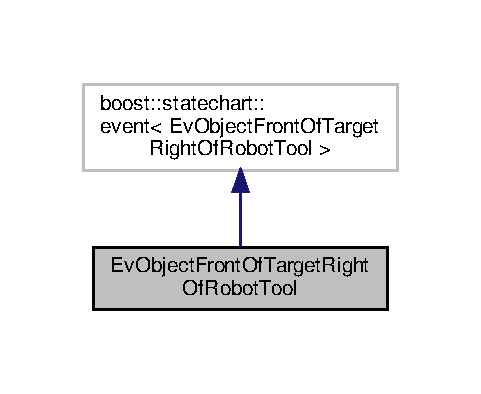
\includegraphics[width=231pt]{structEvObjectFrontOfTargetRightOfRobotTool__inherit__graph}
\end{center}
\end{figure}


Collaboration diagram for Ev\+Object\+Front\+Of\+Target\+Right\+Of\+Robot\+Tool\+:
\nopagebreak
\begin{figure}[H]
\begin{center}
\leavevmode
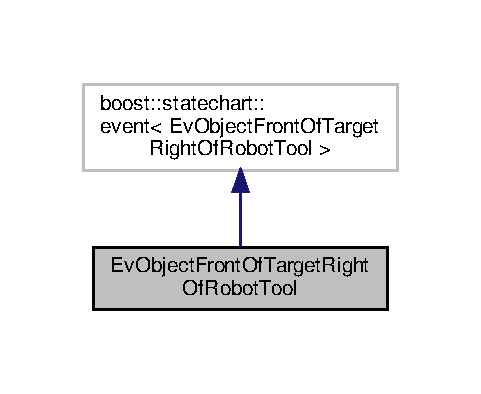
\includegraphics[width=231pt]{structEvObjectFrontOfTargetRightOfRobotTool__coll__graph}
\end{center}
\end{figure}


\subsection{Detailed Description}
State machine Event structure\+: Sequence when object is on the front right of tool. 

The documentation for this struct was generated from the following file\+:\begin{DoxyCompactItemize}
\item 
/home/samuel/\+Desktop/toolcog\+\_\+ws/montecarlo/include/tool\+\_\+expt/\hyperlink{machine_8h}{machine.\+h}\end{DoxyCompactItemize}

\hypertarget{structEvObjectFrontRightOfTargetTool}{}\section{Ev\+Object\+Front\+Right\+Of\+Target\+Tool Struct Reference}
\label{structEvObjectFrontRightOfTargetTool}\index{Ev\+Object\+Front\+Right\+Of\+Target\+Tool@{Ev\+Object\+Front\+Right\+Of\+Target\+Tool}}


State machine Event structure\+: Sequence when object in front right of tool.  




{\ttfamily \#include $<$machine.\+h$>$}



Inheritance diagram for Ev\+Object\+Front\+Right\+Of\+Target\+Tool\+:
\nopagebreak
\begin{figure}[H]
\begin{center}
\leavevmode
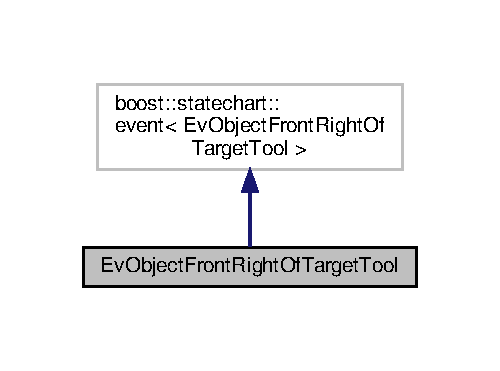
\includegraphics[width=240pt]{structEvObjectFrontRightOfTargetTool__inherit__graph}
\end{center}
\end{figure}


Collaboration diagram for Ev\+Object\+Front\+Right\+Of\+Target\+Tool\+:
\nopagebreak
\begin{figure}[H]
\begin{center}
\leavevmode
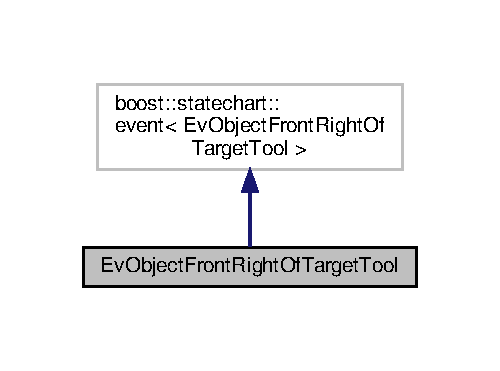
\includegraphics[width=240pt]{structEvObjectFrontRightOfTargetTool__coll__graph}
\end{center}
\end{figure}


\subsection{Detailed Description}
State machine Event structure\+: Sequence when object in front right of tool. 

The documentation for this struct was generated from the following file\+:\begin{DoxyCompactItemize}
\item 
/home/samuel/\+Desktop/toolcog\+\_\+ws/montecarlo/include/tool\+\_\+expt/\hyperlink{machine_8h}{machine.\+h}\end{DoxyCompactItemize}

\hypertarget{structEvObjectRightOfTarget}{}\section{Ev\+Object\+Right\+Of\+Target Struct Reference}
\label{structEvObjectRightOfTarget}\index{Ev\+Object\+Right\+Of\+Target@{Ev\+Object\+Right\+Of\+Target}}


State machine Event structure\+: Sequence when object is on the right side of target goal.  




{\ttfamily \#include $<$machine.\+h$>$}



Inheritance diagram for Ev\+Object\+Right\+Of\+Target\+:
\nopagebreak
\begin{figure}[H]
\begin{center}
\leavevmode
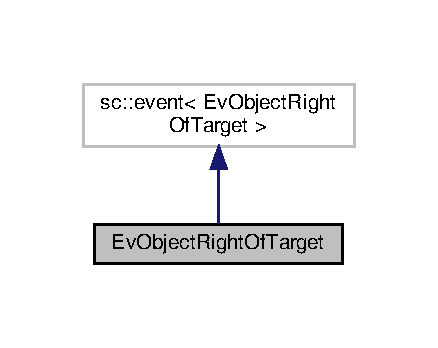
\includegraphics[width=210pt]{structEvObjectRightOfTarget__inherit__graph}
\end{center}
\end{figure}


Collaboration diagram for Ev\+Object\+Right\+Of\+Target\+:
\nopagebreak
\begin{figure}[H]
\begin{center}
\leavevmode
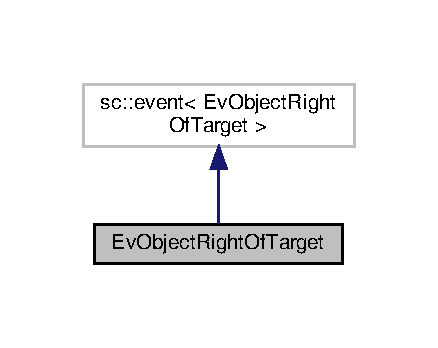
\includegraphics[width=210pt]{structEvObjectRightOfTarget__coll__graph}
\end{center}
\end{figure}


\subsection{Detailed Description}
State machine Event structure\+: Sequence when object is on the right side of target goal. 

The documentation for this struct was generated from the following file\+:\begin{DoxyCompactItemize}
\item 
/home/samuel/\+Desktop/toolcog\+\_\+ws/montecarlo/include/tool\+\_\+expt/\hyperlink{machine_8h}{machine.\+h}\end{DoxyCompactItemize}

\hypertarget{structEvObjectRightOfTargetTool}{}\section{Ev\+Object\+Right\+Of\+Target\+Tool Struct Reference}
\label{structEvObjectRightOfTargetTool}\index{Ev\+Object\+Right\+Of\+Target\+Tool@{Ev\+Object\+Right\+Of\+Target\+Tool}}


State machine Event structure\+: Sequence when object is on the right side of tool.  




{\ttfamily \#include $<$machine.\+h$>$}



Inheritance diagram for Ev\+Object\+Right\+Of\+Target\+Tool\+:
\nopagebreak
\begin{figure}[H]
\begin{center}
\leavevmode
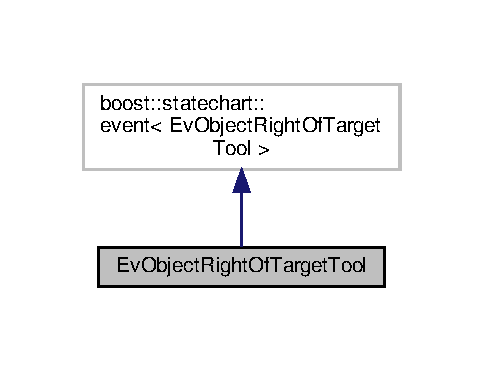
\includegraphics[width=232pt]{structEvObjectRightOfTargetTool__inherit__graph}
\end{center}
\end{figure}


Collaboration diagram for Ev\+Object\+Right\+Of\+Target\+Tool\+:
\nopagebreak
\begin{figure}[H]
\begin{center}
\leavevmode
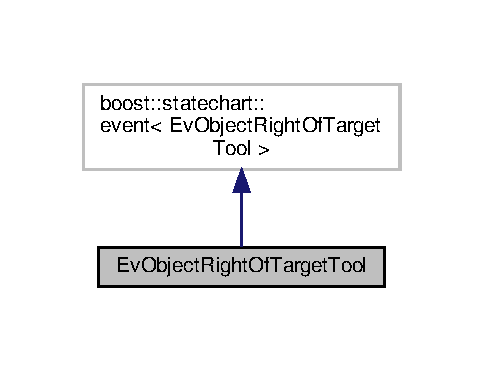
\includegraphics[width=232pt]{structEvObjectRightOfTargetTool__coll__graph}
\end{center}
\end{figure}


\subsection{Detailed Description}
State machine Event structure\+: Sequence when object is on the right side of tool. 

The documentation for this struct was generated from the following file\+:\begin{DoxyCompactItemize}
\item 
/home/samuel/\+Desktop/toolcog\+\_\+ws/montecarlo/include/tool\+\_\+expt/\hyperlink{machine_8h}{machine.\+h}\end{DoxyCompactItemize}

\hypertarget{structEvPerceiveObject}{}\section{Ev\+Perceive\+Object Struct Reference}
\label{structEvPerceiveObject}\index{Ev\+Perceive\+Object@{Ev\+Perceive\+Object}}


State machine Event structure\+: Send request to perception module to detect Object.  




{\ttfamily \#include $<$machine.\+h$>$}



Inheritance diagram for Ev\+Perceive\+Object\+:
\nopagebreak
\begin{figure}[H]
\begin{center}
\leavevmode
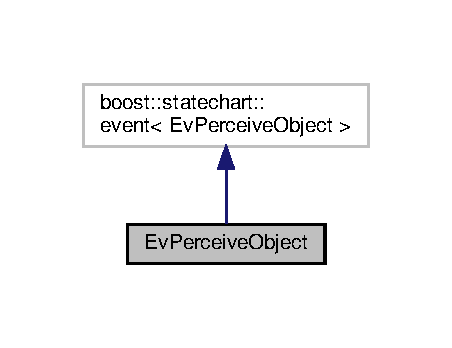
\includegraphics[width=217pt]{structEvPerceiveObject__inherit__graph}
\end{center}
\end{figure}


Collaboration diagram for Ev\+Perceive\+Object\+:
\nopagebreak
\begin{figure}[H]
\begin{center}
\leavevmode
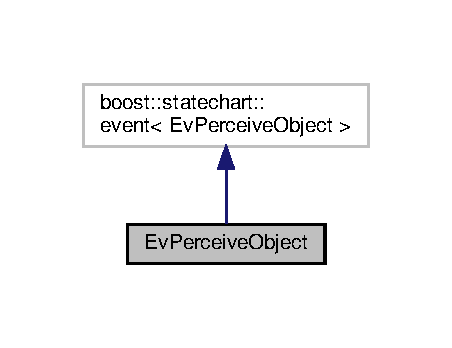
\includegraphics[width=217pt]{structEvPerceiveObject__coll__graph}
\end{center}
\end{figure}


\subsection{Detailed Description}
State machine Event structure\+: Send request to perception module to detect Object. 

The documentation for this struct was generated from the following file\+:\begin{DoxyCompactItemize}
\item 
/home/samuel/\+Desktop/toolcog\+\_\+ws/montecarlo/include/tool\+\_\+expt/\hyperlink{machine_8h}{machine.\+h}\end{DoxyCompactItemize}

\hypertarget{structEvReady}{}\section{Ev\+Ready Struct Reference}
\label{structEvReady}\index{Ev\+Ready@{Ev\+Ready}}


State machine Event structure\+: Ready Sequence.  




{\ttfamily \#include $<$machine.\+h$>$}



Inheritance diagram for Ev\+Ready\+:
\nopagebreak
\begin{figure}[H]
\begin{center}
\leavevmode
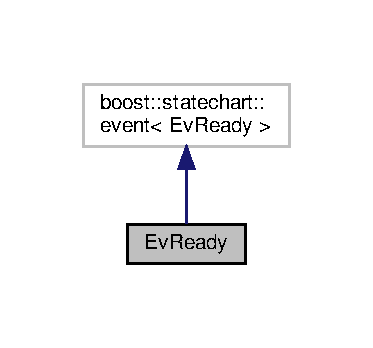
\includegraphics[width=179pt]{structEvReady__inherit__graph}
\end{center}
\end{figure}


Collaboration diagram for Ev\+Ready\+:
\nopagebreak
\begin{figure}[H]
\begin{center}
\leavevmode
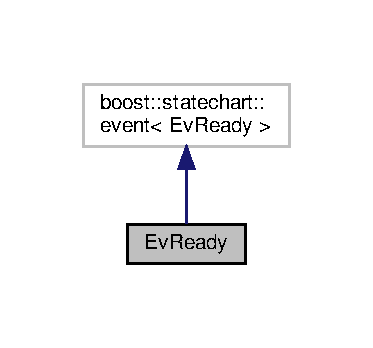
\includegraphics[width=179pt]{structEvReady__coll__graph}
\end{center}
\end{figure}


\subsection{Detailed Description}
State machine Event structure\+: Ready Sequence. 

The documentation for this struct was generated from the following file\+:\begin{DoxyCompactItemize}
\item 
/home/samuel/\+Desktop/toolcog\+\_\+ws/montecarlo/include/tool\+\_\+expt/\hyperlink{machine_8h}{machine.\+h}\end{DoxyCompactItemize}

\hypertarget{structEvStart}{}\section{Ev\+Start Struct Reference}
\label{structEvStart}\index{Ev\+Start@{Ev\+Start}}


State machine Event structure\+: \hyperlink{structStartup}{Startup} sequence \& initialization.  




{\ttfamily \#include $<$machine.\+h$>$}



Inheritance diagram for Ev\+Start\+:
\nopagebreak
\begin{figure}[H]
\begin{center}
\leavevmode
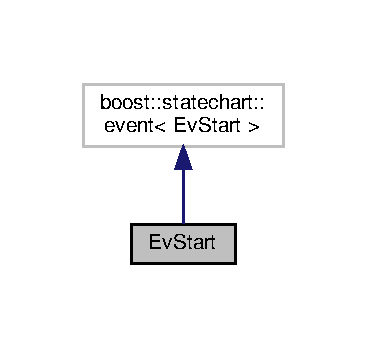
\includegraphics[width=176pt]{structEvStart__inherit__graph}
\end{center}
\end{figure}


Collaboration diagram for Ev\+Start\+:
\nopagebreak
\begin{figure}[H]
\begin{center}
\leavevmode
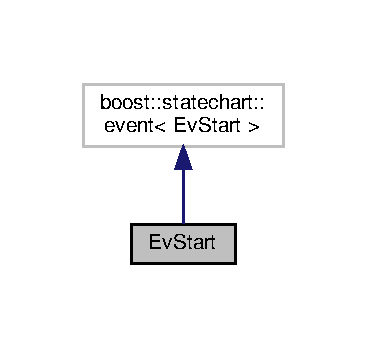
\includegraphics[width=176pt]{structEvStart__coll__graph}
\end{center}
\end{figure}


\subsection{Detailed Description}
State machine Event structure\+: \hyperlink{structStartup}{Startup} sequence \& initialization. 

The documentation for this struct was generated from the following file\+:\begin{DoxyCompactItemize}
\item 
/home/samuel/\+Desktop/toolcog\+\_\+ws/montecarlo/include/tool\+\_\+expt/\hyperlink{machine_8h}{machine.\+h}\end{DoxyCompactItemize}

\hypertarget{structEvTargetNofObject}{}\section{Ev\+Target\+Nof\+Object Struct Reference}
\label{structEvTargetNofObject}\index{Ev\+Target\+Nof\+Object@{Ev\+Target\+Nof\+Object}}


State machine Event structure\+: Sequence when target goal is North of object.  




{\ttfamily \#include $<$machine.\+h$>$}



Inheritance diagram for Ev\+Target\+Nof\+Object\+:
\nopagebreak
\begin{figure}[H]
\begin{center}
\leavevmode
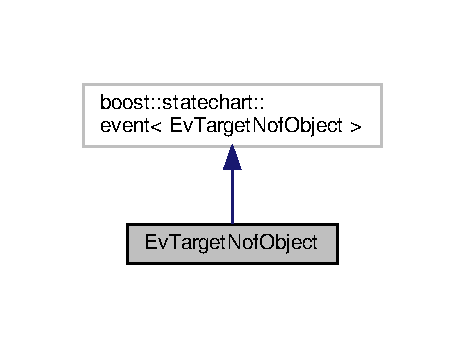
\includegraphics[width=223pt]{structEvTargetNofObject__inherit__graph}
\end{center}
\end{figure}


Collaboration diagram for Ev\+Target\+Nof\+Object\+:
\nopagebreak
\begin{figure}[H]
\begin{center}
\leavevmode
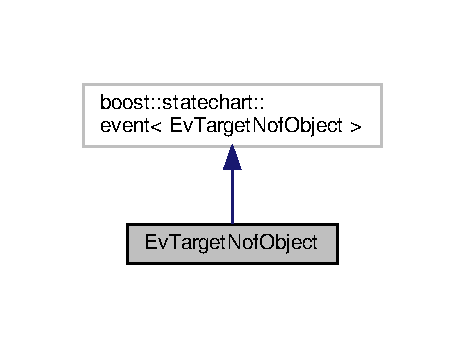
\includegraphics[width=223pt]{structEvTargetNofObject__coll__graph}
\end{center}
\end{figure}


\subsection{Detailed Description}
State machine Event structure\+: Sequence when target goal is North of object. 

The documentation for this struct was generated from the following file\+:\begin{DoxyCompactItemize}
\item 
/home/samuel/\+Desktop/toolcog\+\_\+ws/montecarlo/include/tool\+\_\+expt/\hyperlink{machine_8h}{machine.\+h}\end{DoxyCompactItemize}

\hypertarget{structEvTargetOmniObject}{}\section{Ev\+Target\+Omni\+Object Struct Reference}
\label{structEvTargetOmniObject}\index{Ev\+Target\+Omni\+Object@{Ev\+Target\+Omni\+Object}}


State machine Event structure\+: Based on object position with target, transition into selective event sequences.  




{\ttfamily \#include $<$machine.\+h$>$}



Inheritance diagram for Ev\+Target\+Omni\+Object\+:
\nopagebreak
\begin{figure}[H]
\begin{center}
\leavevmode
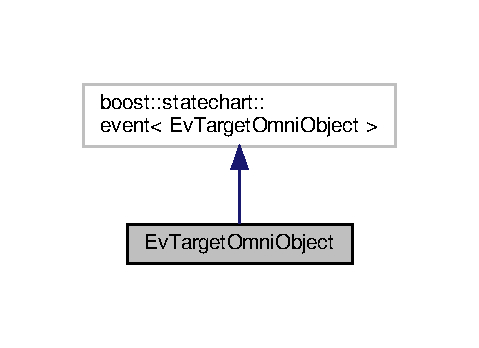
\includegraphics[width=230pt]{structEvTargetOmniObject__inherit__graph}
\end{center}
\end{figure}


Collaboration diagram for Ev\+Target\+Omni\+Object\+:
\nopagebreak
\begin{figure}[H]
\begin{center}
\leavevmode
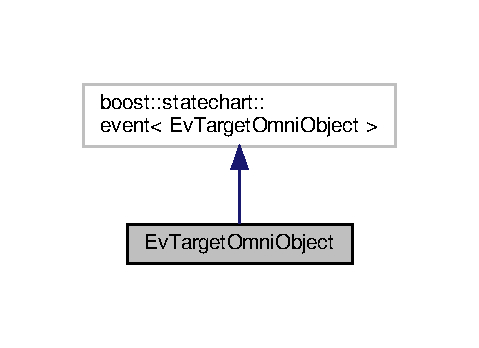
\includegraphics[width=230pt]{structEvTargetOmniObject__coll__graph}
\end{center}
\end{figure}


\subsection{Detailed Description}
State machine Event structure\+: Based on object position with target, transition into selective event sequences. 

The documentation for this struct was generated from the following file\+:\begin{DoxyCompactItemize}
\item 
/home/samuel/\+Desktop/toolcog\+\_\+ws/montecarlo/include/tool\+\_\+expt/\hyperlink{machine_8h}{machine.\+h}\end{DoxyCompactItemize}

\hypertarget{structEvTargetSofObject}{}\section{Ev\+Target\+Sof\+Object Struct Reference}
\label{structEvTargetSofObject}\index{Ev\+Target\+Sof\+Object@{Ev\+Target\+Sof\+Object}}


State machine Event structure\+: Sequence when target goal is South of object.  




{\ttfamily \#include $<$machine.\+h$>$}



Inheritance diagram for Ev\+Target\+Sof\+Object\+:
\nopagebreak
\begin{figure}[H]
\begin{center}
\leavevmode
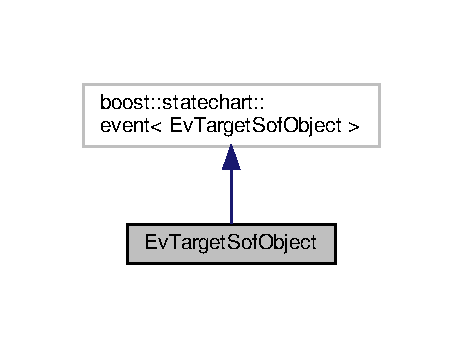
\includegraphics[width=222pt]{structEvTargetSofObject__inherit__graph}
\end{center}
\end{figure}


Collaboration diagram for Ev\+Target\+Sof\+Object\+:
\nopagebreak
\begin{figure}[H]
\begin{center}
\leavevmode
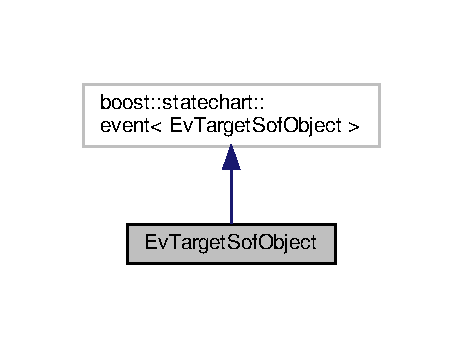
\includegraphics[width=222pt]{structEvTargetSofObject__coll__graph}
\end{center}
\end{figure}


\subsection{Detailed Description}
State machine Event structure\+: Sequence when target goal is South of object. 

The documentation for this struct was generated from the following file\+:\begin{DoxyCompactItemize}
\item 
/home/samuel/\+Desktop/toolcog\+\_\+ws/montecarlo/include/tool\+\_\+expt/\hyperlink{machine_8h}{machine.\+h}\end{DoxyCompactItemize}

\hypertarget{structFunc__Templ}{}\section{Func\+\_\+\+Templ Struct Reference}
\label{structFunc__Templ}\index{Func\+\_\+\+Templ@{Func\+\_\+\+Templ}}


Structure of the function template.  




{\ttfamily \#include $<$tool\+\_\+expt.\+h$>$}

\subsection*{Public Attributes}
\begin{DoxyCompactItemize}
\item 
\mbox{\Hypertarget{structFunc__Templ_a204890a5e37c7857e641536ee921d6cc}\label{structFunc__Templ_a204890a5e37c7857e641536ee921d6cc}} 
Vector3d {\bfseries left}
\item 
\mbox{\Hypertarget{structFunc__Templ_a080467ebb48a80d03bb32a29e30effb3}\label{structFunc__Templ_a080467ebb48a80d03bb32a29e30effb3}} 
Vector3d {\bfseries right}
\item 
\mbox{\Hypertarget{structFunc__Templ_abe4c0c3a70b8a04955dd8ef2c38e86ee}\label{structFunc__Templ_abe4c0c3a70b8a04955dd8ef2c38e86ee}} 
Vector3d {\bfseries normal}
\item 
\mbox{\Hypertarget{structFunc__Templ_ad609bc26b01bf581c94f97475acc0c5c}\label{structFunc__Templ_ad609bc26b01bf581c94f97475acc0c5c}} 
Vector3d {\bfseries objdir}
\item 
\mbox{\Hypertarget{structFunc__Templ_a6145d9afe09af59b6fc7338402fd2316}\label{structFunc__Templ_a6145d9afe09af59b6fc7338402fd2316}} 
Vector3d {\bfseries objpos}
\end{DoxyCompactItemize}


\subsection{Detailed Description}
Structure of the function template. 

The documentation for this struct was generated from the following file\+:\begin{DoxyCompactItemize}
\item 
/home/samuel/\+Desktop/toolcog\+\_\+ws/montecarlo/include/tool\+\_\+expt/\hyperlink{tool__expt_8h}{tool\+\_\+expt.\+h}\end{DoxyCompactItemize}

\hypertarget{classGJK}{}\section{G\+JK Class Reference}
\label{classGJK}\index{G\+JK@{G\+JK}}


\hyperlink{classGJK}{G\+JK} algothrim wrapper Use this class for fast collision check between 2 objects.  




{\ttfamily \#include $<$gjk.\+h$>$}

\subsection*{Public Member Functions}
\begin{DoxyCompactItemize}
\item 
\mbox{\Hypertarget{classGJK_ace7ef0c63a492a9ef896c691a0f8eadc}\label{classGJK_ace7ef0c63a492a9ef896c691a0f8eadc}} 
\hyperlink{classGJK_ace7ef0c63a492a9ef896c691a0f8eadc}{G\+JK} ()
\begin{DoxyCompactList}\small\item\em Construct a new \hyperlink{classGJK}{G\+JK} object. \end{DoxyCompactList}\item 
\mbox{\Hypertarget{classGJK_aa1c552853757d1db1d24d5b43e573e7e}\label{classGJK_aa1c552853757d1db1d24d5b43e573e7e}} 
\hyperlink{classGJK_aa1c552853757d1db1d24d5b43e573e7e}{$\sim$\+G\+JK} ()
\begin{DoxyCompactList}\small\item\em Destroy the \hyperlink{classGJK}{G\+JK} object. \end{DoxyCompactList}\item 
bool \hyperlink{classGJK_aa47f0a72a102236c96251951d5b98c78}{collision\+\_\+check} (\hyperlink{structShape}{Shape} s1, \hyperlink{structShape}{Shape} s2, int iterations)
\begin{DoxyCompactList}\small\item\em collision checking function \end{DoxyCompactList}\end{DoxyCompactItemize}
\subsection*{Private Member Functions}
\begin{DoxyCompactItemize}
\item 
void \hyperlink{classGJK_aba173ffe2b0fc0fb5f2bca0bbe5177ef}{pick\+Line} (\hyperlink{structShape}{Shape} s1, \hyperlink{structShape}{Shape} s2, Vector3d v, Vector3d \&a, Vector3d \&b)
\begin{DoxyCompactList}\small\item\em compute line check \end{DoxyCompactList}\item 
bool \hyperlink{classGJK_a7e843858e96f401c08a97f40171fab0d}{pick\+Triangle} (\hyperlink{structShape}{Shape} s1, \hyperlink{structShape}{Shape} s2, Vector3d \&a, Vector3d \&b, Vector3d \&c)
\begin{DoxyCompactList}\small\item\em Compute Triangle check. \end{DoxyCompactList}\item 
bool \hyperlink{classGJK_a17f529ee6a7ef8fdfd01062523bb97fa}{pick\+Tetrahedron} (\hyperlink{structShape}{Shape} s1, \hyperlink{structShape}{Shape} s2, Vector3d \&a, Vector3d \&b, Vector3d \&c, Vector3d \&d)
\begin{DoxyCompactList}\small\item\em Compute tetrahedron check. \end{DoxyCompactList}\item 
Vector3d \hyperlink{classGJK_abf05bc7c7c1f39f72d582e9eeab5226d}{support} (\hyperlink{structShape}{Shape} s1, \hyperlink{structShape}{Shape} s2, Vector3d v)
\begin{DoxyCompactList}\small\item\em Compute support vector. \end{DoxyCompactList}\item 
Vector3d \hyperlink{classGJK_af4aea563d6d864cc85fafa050a8510eb}{get\+Furthestln\+Dir} (\hyperlink{structShape}{Shape} s1, Vector3d v)
\begin{DoxyCompactList}\small\item\em Get the Furthestln\+Dir object. \end{DoxyCompactList}\end{DoxyCompactItemize}
\subsection*{Private Attributes}
\begin{DoxyCompactItemize}
\item 
\mbox{\Hypertarget{classGJK_a06667bbfe53b1124831d25da58090a01}\label{classGJK_a06667bbfe53b1124831d25da58090a01}} 
int \hyperlink{classGJK_a06667bbfe53b1124831d25da58090a01}{iteration}
\begin{DoxyCompactList}\small\item\em number of iteration used in for the \hyperlink{classGJK}{G\+JK} check \end{DoxyCompactList}\item 
\mbox{\Hypertarget{classGJK_afa9c1221d2268f946a11c2ed42de2acb}\label{classGJK_afa9c1221d2268f946a11c2ed42de2acb}} 
Vector3d \hyperlink{classGJK_afa9c1221d2268f946a11c2ed42de2acb}{vec}
\begin{DoxyCompactList}\small\item\em Weights used for \hyperlink{classGJK}{G\+JK} algorithm. \end{DoxyCompactList}\end{DoxyCompactItemize}


\subsection{Detailed Description}
\hyperlink{classGJK}{G\+JK} algothrim wrapper Use this class for fast collision check between 2 objects. 

\subsection{Member Function Documentation}
\mbox{\Hypertarget{classGJK_aa47f0a72a102236c96251951d5b98c78}\label{classGJK_aa47f0a72a102236c96251951d5b98c78}} 
\index{G\+JK@{G\+JK}!collision\+\_\+check@{collision\+\_\+check}}
\index{collision\+\_\+check@{collision\+\_\+check}!G\+JK@{G\+JK}}
\subsubsection{\texorpdfstring{collision\+\_\+check()}{collision\_check()}}
{\footnotesize\ttfamily bool G\+J\+K\+::collision\+\_\+check (\begin{DoxyParamCaption}\item[{\hyperlink{structShape}{Shape}}]{s1,  }\item[{\hyperlink{structShape}{Shape}}]{s2,  }\item[{int}]{iterations }\end{DoxyParamCaption})}



collision checking function 


\begin{DoxyParams}{Parameters}
{\em s1} & \hyperlink{structShape}{Shape} of object 1 \\
\hline
{\em s2} & \hyperlink{structShape}{Shape} of object 2 \\
\hline
{\em iterations} & number of iterations \\
\hline
\end{DoxyParams}
\begin{DoxyReturn}{Returns}
true = collision detected 

false = no collision 
\end{DoxyReturn}
\mbox{\Hypertarget{classGJK_af4aea563d6d864cc85fafa050a8510eb}\label{classGJK_af4aea563d6d864cc85fafa050a8510eb}} 
\index{G\+JK@{G\+JK}!get\+Furthestln\+Dir@{get\+Furthestln\+Dir}}
\index{get\+Furthestln\+Dir@{get\+Furthestln\+Dir}!G\+JK@{G\+JK}}
\subsubsection{\texorpdfstring{get\+Furthestln\+Dir()}{getFurthestlnDir()}}
{\footnotesize\ttfamily Vector3d G\+J\+K\+::get\+Furthestln\+Dir (\begin{DoxyParamCaption}\item[{\hyperlink{structShape}{Shape}}]{s1,  }\item[{Vector3d}]{v }\end{DoxyParamCaption})\hspace{0.3cm}{\ttfamily [private]}}



Get the Furthestln\+Dir object. 


\begin{DoxyParams}{Parameters}
{\em s1} & shape of object \\
\hline
{\em v} & weight \\
\hline
\end{DoxyParams}
\begin{DoxyReturn}{Returns}
Vector3d Furthest\+Ln\+Dir vector 
\end{DoxyReturn}
\mbox{\Hypertarget{classGJK_aba173ffe2b0fc0fb5f2bca0bbe5177ef}\label{classGJK_aba173ffe2b0fc0fb5f2bca0bbe5177ef}} 
\index{G\+JK@{G\+JK}!pick\+Line@{pick\+Line}}
\index{pick\+Line@{pick\+Line}!G\+JK@{G\+JK}}
\subsubsection{\texorpdfstring{pick\+Line()}{pickLine()}}
{\footnotesize\ttfamily void G\+J\+K\+::pick\+Line (\begin{DoxyParamCaption}\item[{\hyperlink{structShape}{Shape}}]{s1,  }\item[{\hyperlink{structShape}{Shape}}]{s2,  }\item[{Vector3d}]{v,  }\item[{Vector3d \&}]{a,  }\item[{Vector3d \&}]{b }\end{DoxyParamCaption})\hspace{0.3cm}{\ttfamily [private]}}



compute line check 


\begin{DoxyParams}{Parameters}
{\em s1} & shape of object 1 \\
\hline
{\em s2} & shape of object 2 \\
\hline
{\em v} & weight \\
\hline
{\em a} & \\
\hline
{\em b} & \\
\hline
\end{DoxyParams}
\mbox{\Hypertarget{classGJK_a17f529ee6a7ef8fdfd01062523bb97fa}\label{classGJK_a17f529ee6a7ef8fdfd01062523bb97fa}} 
\index{G\+JK@{G\+JK}!pick\+Tetrahedron@{pick\+Tetrahedron}}
\index{pick\+Tetrahedron@{pick\+Tetrahedron}!G\+JK@{G\+JK}}
\subsubsection{\texorpdfstring{pick\+Tetrahedron()}{pickTetrahedron()}}
{\footnotesize\ttfamily bool G\+J\+K\+::pick\+Tetrahedron (\begin{DoxyParamCaption}\item[{\hyperlink{structShape}{Shape}}]{s1,  }\item[{\hyperlink{structShape}{Shape}}]{s2,  }\item[{Vector3d \&}]{a,  }\item[{Vector3d \&}]{b,  }\item[{Vector3d \&}]{c,  }\item[{Vector3d \&}]{d }\end{DoxyParamCaption})\hspace{0.3cm}{\ttfamily [private]}}



Compute tetrahedron check. 


\begin{DoxyParams}{Parameters}
{\em s1} & shape of object 1 \\
\hline
{\em s2} & shape of object 2 \\
\hline
{\em a} & \\
\hline
{\em b} & \\
\hline
{\em c} & \\
\hline
{\em d} & \\
\hline
\end{DoxyParams}
\begin{DoxyReturn}{Returns}
true = collision detected 

false = no collision 
\end{DoxyReturn}
\mbox{\Hypertarget{classGJK_a7e843858e96f401c08a97f40171fab0d}\label{classGJK_a7e843858e96f401c08a97f40171fab0d}} 
\index{G\+JK@{G\+JK}!pick\+Triangle@{pick\+Triangle}}
\index{pick\+Triangle@{pick\+Triangle}!G\+JK@{G\+JK}}
\subsubsection{\texorpdfstring{pick\+Triangle()}{pickTriangle()}}
{\footnotesize\ttfamily bool G\+J\+K\+::pick\+Triangle (\begin{DoxyParamCaption}\item[{\hyperlink{structShape}{Shape}}]{s1,  }\item[{\hyperlink{structShape}{Shape}}]{s2,  }\item[{Vector3d \&}]{a,  }\item[{Vector3d \&}]{b,  }\item[{Vector3d \&}]{c }\end{DoxyParamCaption})\hspace{0.3cm}{\ttfamily [private]}}



Compute Triangle check. 


\begin{DoxyParams}{Parameters}
{\em s1} & shape of object 1 \\
\hline
{\em s2} & shape of object 2 \\
\hline
{\em a} & \\
\hline
{\em b} & \\
\hline
{\em c} & \\
\hline
\end{DoxyParams}
\begin{DoxyReturn}{Returns}
true = collision detected 

false = no collision 
\end{DoxyReturn}
\mbox{\Hypertarget{classGJK_abf05bc7c7c1f39f72d582e9eeab5226d}\label{classGJK_abf05bc7c7c1f39f72d582e9eeab5226d}} 
\index{G\+JK@{G\+JK}!support@{support}}
\index{support@{support}!G\+JK@{G\+JK}}
\subsubsection{\texorpdfstring{support()}{support()}}
{\footnotesize\ttfamily Vector3d G\+J\+K\+::support (\begin{DoxyParamCaption}\item[{\hyperlink{structShape}{Shape}}]{s1,  }\item[{\hyperlink{structShape}{Shape}}]{s2,  }\item[{Vector3d}]{v }\end{DoxyParamCaption})\hspace{0.3cm}{\ttfamily [private]}}



Compute support vector. 


\begin{DoxyParams}{Parameters}
{\em s1} & shape of object 1 \\
\hline
{\em s2} & shape of object 2 \\
\hline
{\em v} & weight vector \\
\hline
\end{DoxyParams}
\begin{DoxyReturn}{Returns}
Vector3d support vector 
\end{DoxyReturn}


The documentation for this class was generated from the following files\+:\begin{DoxyCompactItemize}
\item 
/home/samuel/\+Desktop/toolcog\+\_\+ws/montecarlo/include/tool\+\_\+expt/\hyperlink{gjk_8h}{gjk.\+h}\item 
/home/samuel/\+Desktop/toolcog\+\_\+ws/montecarlo/src/gjk.\+cpp\end{DoxyCompactItemize}

\hypertarget{classKDL__IK}{}\section{K\+D\+L\+\_\+\+IK Class Reference}
\label{classKDL__IK}\index{K\+D\+L\+\_\+\+IK@{K\+D\+L\+\_\+\+IK}}


ik solver using K\+DL for node.\+m R\+OS library usage, K\+DL setup class to quickly solve IK  




{\ttfamily \#include $<$kdl\+\_\+ik.\+h$>$}

\subsection*{Public Member Functions}
\begin{DoxyCompactItemize}
\item 
\mbox{\Hypertarget{classKDL__IK_ab5bc497a769ea4b1fb2b121c2d26a895}\label{classKDL__IK_ab5bc497a769ea4b1fb2b121c2d26a895}} 
\hyperlink{classKDL__IK_ab5bc497a769ea4b1fb2b121c2d26a895}{K\+D\+L\+\_\+\+IK} ()
\begin{DoxyCompactList}\small\item\em Construct a new kdl ik object. \end{DoxyCompactList}\item 
\mbox{\Hypertarget{classKDL__IK_a3e2e2ebd42a8689c5761adbf04414e54}\label{classKDL__IK_a3e2e2ebd42a8689c5761adbf04414e54}} 
\hyperlink{classKDL__IK_a3e2e2ebd42a8689c5761adbf04414e54}{$\sim$\+K\+D\+L\+\_\+\+IK} ()
\begin{DoxyCompactList}\small\item\em Destroy the kdl ik object. \end{DoxyCompactList}\item 
void \hyperlink{classKDL__IK_aa7fb5139673aaa0c24620c51fad7e1d6}{init} (bool right=true)
\begin{DoxyCompactList}\small\item\em initialise kdl ik object K\+DL requires reading the urdf of robot to form a K\+DL tree. Unable to handle tree with more than one branches Hence, separated with a boolean flag for left or right arm branches of the tree. Solves IK fast with mathematics \end{DoxyCompactList}\item 
bool \hyperlink{classKDL__IK_ac5840ffc7f30fd303ab5454d02456c54}{ik\+\_\+solve} (Affine3d target\+\_\+\+KS)
\begin{DoxyCompactList}\small\item\em Function to solve the IK for the given target pose. \end{DoxyCompactList}\item 
Jnt\+Array \hyperlink{classKDL__IK_a1e6c6aeb2f702fe462f593946c120f32}{get\+Desired} ()
\begin{DoxyCompactList}\small\item\em Get the Desired joint values in an array format. \end{DoxyCompactList}\item 
void \hyperlink{classKDL__IK_ad134c076c73720c08a77aaf80f9dfa94}{update} (Jnt\+Array \hyperlink{classKDL__IK_a0b1e97f5d23c79a40986acbf2d1d5472}{joint\+\_\+values})
\begin{DoxyCompactList}\small\item\em update the arm values to given joint array values \end{DoxyCompactList}\item 
\mbox{\Hypertarget{classKDL__IK_a94402e5421e60289a2593164c4c9c8db}\label{classKDL__IK_a94402e5421e60289a2593164c4c9c8db}} 
void \hyperlink{classKDL__IK_a94402e5421e60289a2593164c4c9c8db}{reset} ()
\begin{DoxyCompactList}\small\item\em reset and reinitialise the joint values of the arm to home position this function is used to reset position of K\+DL tree \end{DoxyCompactList}\item 
void \hyperlink{classKDL__IK_ab9717f11ad7991e06ed688ce1c803b85}{init\+\_\+home} (vector$<$ double $>$ \hyperlink{classKDL__IK_a0b1e97f5d23c79a40986acbf2d1d5472}{joint\+\_\+values}, Jnt\+Array max, Jnt\+Array min)
\begin{DoxyCompactList}\small\item\em perform forward kinematics (FK) and store the position of given joint values as the home position \end{DoxyCompactList}\item 
Matrix\+Xd \hyperlink{classKDL__IK_a6560fe32bf60646cb298e9f6751c2d79}{jacobian\+\_\+solve} ()
\begin{DoxyCompactList}\small\item\em solve the jacobian matrix of the K\+DL tree \end{DoxyCompactList}\end{DoxyCompactItemize}
\subsection*{Private Attributes}
\begin{DoxyCompactItemize}
\item 
\mbox{\Hypertarget{classKDL__IK_ab88c264c531d047146dd6042619ccc11}\label{classKDL__IK_ab88c264c531d047146dd6042619ccc11}} 
K\+D\+L\+::\+Tree \hyperlink{classKDL__IK_ab88c264c531d047146dd6042619ccc11}{my\+\_\+tree}
\begin{DoxyCompactList}\small\item\em store the K\+DL tree \end{DoxyCompactList}\item 
\mbox{\Hypertarget{classKDL__IK_a5bfdf9991aecb31a19c542ed3e00445c}\label{classKDL__IK_a5bfdf9991aecb31a19c542ed3e00445c}} 
K\+D\+L\+::\+Chain \hyperlink{classKDL__IK_a5bfdf9991aecb31a19c542ed3e00445c}{arm\+\_\+chain}
\begin{DoxyCompactList}\small\item\em store the kdl chain up to the arm \end{DoxyCompactList}\item 
\mbox{\Hypertarget{classKDL__IK_a108760856d54cff9d178c5cd7fed56dc}\label{classKDL__IK_a108760856d54cff9d178c5cd7fed56dc}} 
K\+D\+L\+::\+Chain \hyperlink{classKDL__IK_a108760856d54cff9d178c5cd7fed56dc}{R\+S\+\_\+chain}
\begin{DoxyCompactList}\small\item\em store the kdl chain up to the right shoulder (RS) \end{DoxyCompactList}\item 
\mbox{\Hypertarget{classKDL__IK_a0b1e97f5d23c79a40986acbf2d1d5472}\label{classKDL__IK_a0b1e97f5d23c79a40986acbf2d1d5472}} 
std\+::vector$<$ double $>$ \hyperlink{classKDL__IK_a0b1e97f5d23c79a40986acbf2d1d5472}{joint\+\_\+values}
\begin{DoxyCompactList}\small\item\em store the joint values \end{DoxyCompactList}\item 
\mbox{\Hypertarget{classKDL__IK_ae5ce6ddb1594093232d33b3dc8b222ed}\label{classKDL__IK_ae5ce6ddb1594093232d33b3dc8b222ed}} 
Jnt\+Array \hyperlink{classKDL__IK_ae5ce6ddb1594093232d33b3dc8b222ed}{arm\+Angles\+\_\+\+Home}
\begin{DoxyCompactList}\small\item\em store the arm values for \textquotesingle{}Home\textquotesingle{} position \end{DoxyCompactList}\item 
\mbox{\Hypertarget{classKDL__IK_a69b2c6c67e16aaec8a87b038361193e2}\label{classKDL__IK_a69b2c6c67e16aaec8a87b038361193e2}} 
Jnt\+Array \hyperlink{classKDL__IK_a69b2c6c67e16aaec8a87b038361193e2}{arm\+Angles}
\begin{DoxyCompactList}\small\item\em store the current arm joint values \end{DoxyCompactList}\item 
\mbox{\Hypertarget{classKDL__IK_a11e0fd66cf9eb471f7041162d5c98004}\label{classKDL__IK_a11e0fd66cf9eb471f7041162d5c98004}} 
Jnt\+Array \hyperlink{classKDL__IK_a11e0fd66cf9eb471f7041162d5c98004}{R\+S\+Angles}
\begin{DoxyCompactList}\small\item\em store the current right shoulder(\+R\+S) joint values \end{DoxyCompactList}\item 
\mbox{\Hypertarget{classKDL__IK_a7fb4557cb3d9e1bc2cd9aab192b824d3}\label{classKDL__IK_a7fb4557cb3d9e1bc2cd9aab192b824d3}} 
Jnt\+Array \hyperlink{classKDL__IK_a7fb4557cb3d9e1bc2cd9aab192b824d3}{arm\+Angles\+\_\+d}
\begin{DoxyCompactList}\small\item\em store the delta (difference) of each joint in the arm \end{DoxyCompactList}\item 
\mbox{\Hypertarget{classKDL__IK_a27043e37e4187ab9a69b2fa4ed6743b7}\label{classKDL__IK_a27043e37e4187ab9a69b2fa4ed6743b7}} 
Affine3d \hyperlink{classKDL__IK_a27043e37e4187ab9a69b2fa4ed6743b7}{R\+S\+\_\+\+KS}
\begin{DoxyCompactList}\small\item\em store the Right shoulder (RS) kinematics solution (KS) \end{DoxyCompactList}\item 
\mbox{\Hypertarget{classKDL__IK_a3c1c05b65f0f06348fc234e928147ca8}\label{classKDL__IK_a3c1c05b65f0f06348fc234e928147ca8}} 
int \hyperlink{classKDL__IK_a3c1c05b65f0f06348fc234e928147ca8}{arm\+\_\+no}
\begin{DoxyCompactList}\small\item\em the arm\textquotesingle{}s number \end{DoxyCompactList}\item 
\mbox{\Hypertarget{classKDL__IK_ade06f6d5bdbce0b39b12061fb767dafa}\label{classKDL__IK_ade06f6d5bdbce0b39b12061fb767dafa}} 
int \hyperlink{classKDL__IK_ade06f6d5bdbce0b39b12061fb767dafa}{rs\+\_\+no}
\begin{DoxyCompactList}\small\item\em the right shoulder number \end{DoxyCompactList}\item 
\mbox{\Hypertarget{classKDL__IK_ace94ad54266c4b7099659dfabbb2a342}\label{classKDL__IK_ace94ad54266c4b7099659dfabbb2a342}} 
Jnt\+Array \hyperlink{classKDL__IK_ace94ad54266c4b7099659dfabbb2a342}{max\+Jnt}
\begin{DoxyCompactList}\small\item\em store the maximum and minimum values of each joint \end{DoxyCompactList}\item 
\mbox{\Hypertarget{classKDL__IK_a3d9d9c11cf2847ae6a85e8241c7885e8}\label{classKDL__IK_a3d9d9c11cf2847ae6a85e8241c7885e8}} 
Jnt\+Array {\bfseries min\+Jnt}
\end{DoxyCompactItemize}


\subsection{Detailed Description}
ik solver using K\+DL for node.\+m R\+OS library usage, K\+DL setup class to quickly solve IK 

\subsection{Member Function Documentation}
\mbox{\Hypertarget{classKDL__IK_a1e6c6aeb2f702fe462f593946c120f32}\label{classKDL__IK_a1e6c6aeb2f702fe462f593946c120f32}} 
\index{K\+D\+L\+\_\+\+IK@{K\+D\+L\+\_\+\+IK}!get\+Desired@{get\+Desired}}
\index{get\+Desired@{get\+Desired}!K\+D\+L\+\_\+\+IK@{K\+D\+L\+\_\+\+IK}}
\subsubsection{\texorpdfstring{get\+Desired()}{getDesired()}}
{\footnotesize\ttfamily Jnt\+Array K\+D\+L\+\_\+\+I\+K\+::get\+Desired (\begin{DoxyParamCaption}{ }\end{DoxyParamCaption})\hspace{0.3cm}{\ttfamily [inline]}}



Get the Desired joint values in an array format. 

\begin{DoxyReturn}{Returns}
Jnt\+Array K\+DL joint array data format 
\end{DoxyReturn}
\mbox{\Hypertarget{classKDL__IK_ac5840ffc7f30fd303ab5454d02456c54}\label{classKDL__IK_ac5840ffc7f30fd303ab5454d02456c54}} 
\index{K\+D\+L\+\_\+\+IK@{K\+D\+L\+\_\+\+IK}!ik\+\_\+solve@{ik\+\_\+solve}}
\index{ik\+\_\+solve@{ik\+\_\+solve}!K\+D\+L\+\_\+\+IK@{K\+D\+L\+\_\+\+IK}}
\subsubsection{\texorpdfstring{ik\+\_\+solve()}{ik\_solve()}}
{\footnotesize\ttfamily bool K\+D\+L\+\_\+\+I\+K\+::ik\+\_\+solve (\begin{DoxyParamCaption}\item[{Affine3d}]{target\+\_\+\+KS }\end{DoxyParamCaption})\hspace{0.3cm}{\ttfamily [inline]}}



Function to solve the IK for the given target pose. 


\begin{DoxyParams}{Parameters}
{\em target\+\_\+\+KS} & Affine matrix for the target \\
\hline
\end{DoxyParams}
\begin{DoxyReturn}{Returns}
true IK solved successfully 

false error encountered 
\end{DoxyReturn}
\mbox{\Hypertarget{classKDL__IK_aa7fb5139673aaa0c24620c51fad7e1d6}\label{classKDL__IK_aa7fb5139673aaa0c24620c51fad7e1d6}} 
\index{K\+D\+L\+\_\+\+IK@{K\+D\+L\+\_\+\+IK}!init@{init}}
\index{init@{init}!K\+D\+L\+\_\+\+IK@{K\+D\+L\+\_\+\+IK}}
\subsubsection{\texorpdfstring{init()}{init()}}
{\footnotesize\ttfamily void K\+D\+L\+\_\+\+I\+K\+::init (\begin{DoxyParamCaption}\item[{bool}]{right = {\ttfamily true} }\end{DoxyParamCaption})\hspace{0.3cm}{\ttfamily [inline]}}



initialise kdl ik object K\+DL requires reading the urdf of robot to form a K\+DL tree. Unable to handle tree with more than one branches Hence, separated with a boolean flag for left or right arm branches of the tree. Solves IK fast with mathematics 


\begin{DoxyParams}{Parameters}
{\em right} & true = right arm of olivia, false = left arm of olivia \\
\hline
\end{DoxyParams}
\mbox{\Hypertarget{classKDL__IK_ab9717f11ad7991e06ed688ce1c803b85}\label{classKDL__IK_ab9717f11ad7991e06ed688ce1c803b85}} 
\index{K\+D\+L\+\_\+\+IK@{K\+D\+L\+\_\+\+IK}!init\+\_\+home@{init\+\_\+home}}
\index{init\+\_\+home@{init\+\_\+home}!K\+D\+L\+\_\+\+IK@{K\+D\+L\+\_\+\+IK}}
\subsubsection{\texorpdfstring{init\+\_\+home()}{init\_home()}}
{\footnotesize\ttfamily void K\+D\+L\+\_\+\+I\+K\+::init\+\_\+home (\begin{DoxyParamCaption}\item[{vector$<$ double $>$}]{joint\+\_\+values,  }\item[{Jnt\+Array}]{max,  }\item[{Jnt\+Array}]{min }\end{DoxyParamCaption})\hspace{0.3cm}{\ttfamily [inline]}}



perform forward kinematics (FK) and store the position of given joint values as the home position 


\begin{DoxyParams}{Parameters}
{\em joint\+\_\+values} & the given joint values \\
\hline
{\em max} & Maximum value of each joints \\
\hline
{\em min} & Minimum value of each joints \\
\hline
\end{DoxyParams}
\mbox{\Hypertarget{classKDL__IK_a6560fe32bf60646cb298e9f6751c2d79}\label{classKDL__IK_a6560fe32bf60646cb298e9f6751c2d79}} 
\index{K\+D\+L\+\_\+\+IK@{K\+D\+L\+\_\+\+IK}!jacobian\+\_\+solve@{jacobian\+\_\+solve}}
\index{jacobian\+\_\+solve@{jacobian\+\_\+solve}!K\+D\+L\+\_\+\+IK@{K\+D\+L\+\_\+\+IK}}
\subsubsection{\texorpdfstring{jacobian\+\_\+solve()}{jacobian\_solve()}}
{\footnotesize\ttfamily Matrix\+Xd K\+D\+L\+\_\+\+I\+K\+::jacobian\+\_\+solve (\begin{DoxyParamCaption}{ }\end{DoxyParamCaption})\hspace{0.3cm}{\ttfamily [inline]}}



solve the jacobian matrix of the K\+DL tree 

\begin{DoxyReturn}{Returns}
Matrix\+Xd jacobian matrix 
\end{DoxyReturn}
\mbox{\Hypertarget{classKDL__IK_ad134c076c73720c08a77aaf80f9dfa94}\label{classKDL__IK_ad134c076c73720c08a77aaf80f9dfa94}} 
\index{K\+D\+L\+\_\+\+IK@{K\+D\+L\+\_\+\+IK}!update@{update}}
\index{update@{update}!K\+D\+L\+\_\+\+IK@{K\+D\+L\+\_\+\+IK}}
\subsubsection{\texorpdfstring{update()}{update()}}
{\footnotesize\ttfamily void K\+D\+L\+\_\+\+I\+K\+::update (\begin{DoxyParamCaption}\item[{Jnt\+Array}]{joint\+\_\+values }\end{DoxyParamCaption})\hspace{0.3cm}{\ttfamily [inline]}}



update the arm values to given joint array values 


\begin{DoxyParams}{Parameters}
{\em joint\+\_\+values} & K\+DL joint array data format \\
\hline
\end{DoxyParams}


The documentation for this class was generated from the following file\+:\begin{DoxyCompactItemize}
\item 
/home/samuel/\+Desktop/toolcog\+\_\+ws/montecarlo/include/tool\+\_\+expt/\hyperlink{kdl__ik_8h}{kdl\+\_\+ik.\+h}\end{DoxyCompactItemize}

\hypertarget{classM3MoveGroup}{}\section{M3\+Move\+Group Class Reference}
\label{classM3MoveGroup}\index{M3\+Move\+Group@{M3\+Move\+Group}}


Moveit action server.  


\subsection*{Public Member Functions}
\begin{DoxyCompactItemize}
\item 
\mbox{\Hypertarget{classM3MoveGroup_aeb66c992c2a648e53f823a6058669c4c}\label{classM3MoveGroup_aeb66c992c2a648e53f823a6058669c4c}} 
{\bfseries M3\+Move\+Group} (std\+::string name)
\item 
void \hyperlink{classM3MoveGroup_a0d53e8cfafd00e1a22f1cf5e091b63a1}{Input\+Callback} (const std\+\_\+msgs\+::\+Int32\+Const\+Ptr \&input)
\begin{DoxyCompactList}\small\item\em user input function \end{DoxyCompactList}\item 
void \hyperlink{classM3MoveGroup_a754821f89a28e5b3e6924d9f9e040946}{finger\+Timeout\+Callback} (const std\+\_\+msgs\+::\+Bool timeout)
\begin{DoxyCompactList}\small\item\em action server timeout callback for finger \end{DoxyCompactList}\item 
void \hyperlink{classM3MoveGroup_a78c1d36f86d5ade3dc73b6239227a512}{finger\+Timer\+Timeout\+Callback} (const ros\+::\+Timer\+Event \&e)
\begin{DoxyCompactList}\small\item\em Using ros timer to check for finger timeout. \end{DoxyCompactList}\item 
void \hyperlink{classM3MoveGroup_ada2b7b9e5a402676eff8747267385f6b}{Collision\+Object\+Callback} (const moveit\+\_\+msgs\+::\+Collision\+Object\+Const\+Ptr \&obj)
\begin{DoxyCompactList}\small\item\em Action server to add collision object into moveit planning scene. \end{DoxyCompactList}\item 
void \hyperlink{classM3MoveGroup_a9b982c9f3cd26755ed9b6ecca1286c50}{callback\+\_\+testpub} (const ros\+::\+Timer\+Event \&e)
\begin{DoxyCompactList}\small\item\em callback test for fingers \end{DoxyCompactList}\item 
void \hyperlink{classM3MoveGroup_a1a515c13453033a4ab89b5599d58f23f}{callback\+\_\+stop\+\_\+fingers} (const ros\+::\+Timer\+Event \&e)
\begin{DoxyCompactList}\small\item\em callback to stop fingers. Time based control of olivia fingers \end{DoxyCompactList}\item 
void \hyperlink{classM3MoveGroup_af7c4ca891be62a8c3fdb7cd0cc0cb2a0}{callback\+\_\+stop\+\_\+fingers1} (const ros\+::\+Timer\+Event \&e)
\begin{DoxyCompactList}\small\item\em time-\/based control to stop olivia finger1 \end{DoxyCompactList}\item 
void \hyperlink{classM3MoveGroup_af6a7a1d4aab641328a9213689f7b9ce1}{callback\+\_\+stop\+\_\+fingers2} (const ros\+::\+Timer\+Event \&e)
\begin{DoxyCompactList}\small\item\em time based control to stop olivia finger2 \end{DoxyCompactList}\item 
void \hyperlink{classM3MoveGroup_aedb5d4a4aaeebd2ef3fa0d54edb0efaa}{stop\+\_\+fingers} (std\+::vector$<$ std\+::string $>$ names)
\begin{DoxyCompactList}\small\item\em time based control to stop all olivia fingers \end{DoxyCompactList}\item 
void \hyperlink{classM3MoveGroup_a7208ba7725391ea9ffd98d3d31ae5f0d}{Finger\+Encoder\+Callback} (const kaist\+\_\+msgs\+::\+Joint\+Encoder\+Status\+Const\+Ptr \&joint)
\begin{DoxyCompactList}\small\item\em encoder position based control to stop olivia fingers \end{DoxyCompactList}\item 
void \hyperlink{classM3MoveGroup_ab202574f8621d26c6369c1b794014251}{Fingers\+Encoders\+Action\+CB} (const m3\+\_\+moveit\+::\+Moveit\+Fingers\+Goal\+Const\+Ptr \&goal)
\begin{DoxyCompactList}\small\item\em action server to control olivia fingers using encoders \end{DoxyCompactList}\item 
void \hyperlink{classM3MoveGroup_a50f3c0ec424696c8d613cbfb18829384}{Fingers\+Action\+CB} (const m3\+\_\+moveit\+::\+Moveit\+Fingers\+Goal\+Const\+Ptr \&goal)
\begin{DoxyCompactList}\small\item\em Action server to control olivia fingers. \end{DoxyCompactList}\item 
void \hyperlink{classM3MoveGroup_a71fc79c75e8e96881d0cfa6629f5e11d}{Cart\+Single\+Action\+CB} (const m3\+\_\+moveit\+::\+Moveit\+Single\+Goal\+Const\+Ptr \&goal)
\begin{DoxyCompactList}\small\item\em Moveit action server\+: planning using cartesian space for single arm. \end{DoxyCompactList}\item 
void \hyperlink{classM3MoveGroup_a6ce4ef5d30fc1e93826f4f8104f8db04}{Cart\+Single\+Right\+Action\+CB} (const m3\+\_\+moveit\+::\+Moveit\+Single\+Goal\+Const\+Ptr \&goal)
\begin{DoxyCompactList}\small\item\em Moveit Action server\+: Using cartesian space planning for single right arm. \end{DoxyCompactList}\item 
double \hyperlink{classM3MoveGroup_a08ae3af12542a9dd44d5f823c8b3bb46}{r2d} (double rad)
\begin{DoxyCompactList}\small\item\em radian to degree conversion \end{DoxyCompactList}\item 
std\+::vector$<$ double $>$ \hyperlink{classM3MoveGroup_a76eed72085b10fa6fea6f9cc773a7901}{Convert\+To\+Olivia\+Coordinates} (const std\+::vector$<$ double $>$ input)
\begin{DoxyCompactList}\small\item\em Remap and convert joint angles to Olivia differences in real robot and urdf, this is to remap the joints before sending to real robot. \end{DoxyCompactList}\item 
std\+::vector$<$ double $>$ \hyperlink{classM3MoveGroup_a59d8555d6560673417be20d6bf5d6aae}{Convert\+To\+Olivia\+Head} (const std\+::vector$<$ double $>$ input)
\begin{DoxyCompactList}\small\item\em Remap and convert joint angles to Olivia A separate dynamixel is used for the head. Joint value need to be send separately. \end{DoxyCompactList}\item 
std\+::vector$<$ double $>$ \hyperlink{classM3MoveGroup_a422eebf405bc0b3187bb6e692b361fa0}{Convert\+Olivia\+Arm} (const std\+::vector$<$ double $>$ input, std\+::string arm)
\begin{DoxyCompactList}\small\item\em Remap and convert joint angles to Olivia (for the arm only) \end{DoxyCompactList}\item 
void \hyperlink{classM3MoveGroup_a0b0b4680d729b8878a89ba03c6d59303}{Send2\+Olivia\+Single\+Arm} (moveit\+\_\+msgs\+::\+Robot\+Trajectory trajectory, std\+::string link\+\_\+name)
\begin{DoxyCompactList}\small\item\em send joint values to kaist daemon to move real olivia \end{DoxyCompactList}\item 
void \hyperlink{classM3MoveGroup_a8adcfcf74c2e2350189be855dca572de}{Send2\+Olivia\+Whole\+Body} (moveit\+\_\+msgs\+::\+Robot\+Trajectory trajectory)
\begin{DoxyCompactList}\small\item\em send joint values to kaist daemon to move real olivia (for whole body) \end{DoxyCompactList}\item 
void \hyperlink{classM3MoveGroup_a5f4c7d0260a2d987e5abaf1b1365c657}{Send2\+Olivia\+Head} (moveit\+\_\+msgs\+::\+Robot\+Trajectory trajectory)
\begin{DoxyCompactList}\small\item\em send joint values to dynamixel to move real olivia head only \end{DoxyCompactList}\item 
void \hyperlink{classM3MoveGroup_a5cbdff90f02f8067d55c1b4592b24b72}{Task\+Single\+Action\+CB} (const m3\+\_\+moveit\+::\+Moveit\+Single\+Goal\+Const\+Ptr \&goal)
\begin{DoxyCompactList}\small\item\em Moveit Action server\+: moveit group task planning, movement less predictable, but higher rate of success. \end{DoxyCompactList}\item 
void \hyperlink{classM3MoveGroup_aee17065b5aa40384dcca5a6589261ded}{Task\+Single\+Right\+Action\+CB} (const m3\+\_\+moveit\+::\+Moveit\+Single\+Goal\+Const\+Ptr \&goal)
\begin{DoxyCompactList}\small\item\em Moveit Action server\+: moveit group task planning (for right single arm only) \end{DoxyCompactList}\item 
void \hyperlink{classM3MoveGroup_abbc7367f21a594bd3ae7a91fe6441480}{Attach\+Right\+Action\+CB} (const m3\+\_\+moveit\+::\+Moveit\+Pick\+Place\+Goal\+Const\+Ptr \&goal)
\begin{DoxyCompactList}\small\item\em Moveit Action server\+: attaching objects in planning scene to arm (works for both left or right) \end{DoxyCompactList}\item 
void \hyperlink{classM3MoveGroup_a0e43c201d45fd9d987dd5b57f57e6402}{Detach\+Right\+Action\+CB} (const m3\+\_\+moveit\+::\+Moveit\+Pick\+Place\+Goal\+Const\+Ptr \&goal)
\begin{DoxyCompactList}\small\item\em Moveit Action server\+: detach objects in planning scene from arm (works for both left or right) \end{DoxyCompactList}\item 
void \hyperlink{classM3MoveGroup_afad468e11f51e093ef704ebe974ecc28}{Remove\+Collision\+Action\+CB} (const m3\+\_\+moveit\+::\+Moveit\+Collide\+Goal\+Const\+Ptr \&goal)
\begin{DoxyCompactList}\small\item\em Moveit Action server\+: Remove objects from planning scene. \end{DoxyCompactList}\item 
void \hyperlink{classM3MoveGroup_aa1aa80c1a53d3829ed0e535f728cbe63}{Add\+Collision\+Action\+CB} (const m3\+\_\+moveit\+::\+Moveit\+Collide\+Goal\+Const\+Ptr \&goal)
\begin{DoxyCompactList}\small\item\em Moveit Action server\+: add object into planning scene for collision-\/free planning. \end{DoxyCompactList}\item 
void \hyperlink{classM3MoveGroup_a4999726d3def40e06217e81fb7f095ab}{Task\+Dual\+Action\+CB} (const m3\+\_\+moveit\+::\+Moveit\+Dual\+Goal\+Const\+Ptr \&goal)
\begin{DoxyCompactList}\small\item\em Moveit Action server\+: group task planning for both arms. \end{DoxyCompactList}\item 
void \hyperlink{classM3MoveGroup_a3cb5511476fb082b891ac3de867ee8b8}{Mixed\+Whole\+Body\+Action\+CB} (const m3\+\_\+moveit\+::\+Moveit\+Whole\+Body\+Goal\+Const\+Ptr \&goal)
\begin{DoxyCompactList}\small\item\em Moveit Action server\+: joint space planning for whole body. \end{DoxyCompactList}\item 
void \hyperlink{classM3MoveGroup_adcf08e40ebf2191e9d717e2baf275f18}{Joint\+Whole\+Body\+Action\+CB} (const m3\+\_\+moveit\+::\+Moveit\+Whole\+Body\+Goal\+Const\+Ptr \&goal)
\begin{DoxyCompactList}\small\item\em Moveit Action server\+: joint space planning. \end{DoxyCompactList}\item 
\mbox{\Hypertarget{classM3MoveGroup_aef5fd5bd7565b10b0e5d568bce824773}\label{classM3MoveGroup_aef5fd5bd7565b10b0e5d568bce824773}} 
void {\bfseries Neck\+Single\+Action\+CB} (const m3\+\_\+moveit\+::\+Neck\+Tilt\+Goal\+Const\+Ptr \&goal)
\item 
bool \hyperlink{classM3MoveGroup_a65ac544bc2275fc3823bc66c3a2a7a19}{Check\+Hand\+Orientation} (const moveit\+::planning\+\_\+interface\+::\+Move\+Group\+::\+Plan plan, const geometry\+\_\+msgs\+::\+Pose pose\+\_\+left, const geometry\+\_\+msgs\+::\+Pose pose\+\_\+right)
\begin{DoxyCompactList}\small\item\em check the planning scene kinematics models for hand orientation \end{DoxyCompactList}\item 
bool \hyperlink{classM3MoveGroup_a89b6d3658b6884d6a19a2975193e444a}{Check\+Hand\+Orientation} (const moveit\+::planning\+\_\+interface\+::\+Move\+Group\+::\+Plan plan, const geometry\+\_\+msgs\+::\+Pose pose, std\+::string name)
\begin{DoxyCompactList}\small\item\em check the hand orientation in moveit planning \end{DoxyCompactList}\item 
double \hyperlink{classM3MoveGroup_a000211da0f2ad520583f9efff2401e7a}{Get\+Quaternion\+Distance} (std\+::vector$<$ double $>$ quat1, std\+::vector$<$ double $>$ quat2)
\begin{DoxyCompactList}\small\item\em Get the delta distance between 2 quaternion. \end{DoxyCompactList}\item 
void \hyperlink{classM3MoveGroup_adf12117d8738588cadfa6ab62e008fea}{Jiggle\+Target} (int i\+Attempt, geometry\+\_\+msgs\+::\+Pose pose, std\+::string name)
\begin{DoxyCompactList}\small\item\em Attempt to jiggle the target pose to achieve higher success rate when moveit fails to plan. \end{DoxyCompactList}\item 
void \hyperlink{classM3MoveGroup_a01c4d2e768a050ad0652ecc2b612946c}{Jiggle\+Target} (int i\+Attempt, geometry\+\_\+msgs\+::\+Pose pose\+\_\+left, geometry\+\_\+msgs\+::\+Pose pose\+\_\+right, std\+::string name\+\_\+left, std\+::string name\+\_\+right)
\begin{DoxyCompactList}\small\item\em Attempt to jiggle the target pose to achieve higher success rate when moveit fails to plan. \end{DoxyCompactList}\item 
\hyperlink{classM3MoveGroup_aeb66c992c2a648e53f823a6058669c4c}{M3\+Move\+Group} (std\+::string name)
\begin{DoxyCompactList}\small\item\em Construct a new \hyperlink{classM3MoveGroup}{M3\+Move\+Group} object. \end{DoxyCompactList}\item 
void \hyperlink{classM3MoveGroup_a0d53e8cfafd00e1a22f1cf5e091b63a1}{Input\+Callback} (const std\+\_\+msgs\+::\+Int32\+Const\+Ptr \&input)
\begin{DoxyCompactList}\small\item\em user input function \end{DoxyCompactList}\item 
void \hyperlink{classM3MoveGroup_a754821f89a28e5b3e6924d9f9e040946}{finger\+Timeout\+Callback} (const std\+\_\+msgs\+::\+Bool timeout)
\begin{DoxyCompactList}\small\item\em action server timeout callback for finger \end{DoxyCompactList}\item 
void \hyperlink{classM3MoveGroup_a78c1d36f86d5ade3dc73b6239227a512}{finger\+Timer\+Timeout\+Callback} (const ros\+::\+Timer\+Event \&e)
\begin{DoxyCompactList}\small\item\em Using ros timer to check for finger timeout. \end{DoxyCompactList}\item 
void \hyperlink{classM3MoveGroup_ada2b7b9e5a402676eff8747267385f6b}{Collision\+Object\+Callback} (const moveit\+\_\+msgs\+::\+Collision\+Object\+Const\+Ptr \&obj)
\begin{DoxyCompactList}\small\item\em Action server to add collision object into moveit planning scene. \end{DoxyCompactList}\item 
void \hyperlink{classM3MoveGroup_a9b982c9f3cd26755ed9b6ecca1286c50}{callback\+\_\+testpub} (const ros\+::\+Timer\+Event \&e)
\begin{DoxyCompactList}\small\item\em callback test for fingers \end{DoxyCompactList}\item 
void \hyperlink{classM3MoveGroup_a1a515c13453033a4ab89b5599d58f23f}{callback\+\_\+stop\+\_\+fingers} (const ros\+::\+Timer\+Event \&e)
\begin{DoxyCompactList}\small\item\em callback to stop fingers. Time based control of olivia fingers \end{DoxyCompactList}\item 
void \hyperlink{classM3MoveGroup_af7c4ca891be62a8c3fdb7cd0cc0cb2a0}{callback\+\_\+stop\+\_\+fingers1} (const ros\+::\+Timer\+Event \&e)
\begin{DoxyCompactList}\small\item\em time-\/based control to stop olivia finger1 \end{DoxyCompactList}\item 
void \hyperlink{classM3MoveGroup_af6a7a1d4aab641328a9213689f7b9ce1}{callback\+\_\+stop\+\_\+fingers2} (const ros\+::\+Timer\+Event \&e)
\begin{DoxyCompactList}\small\item\em time based control to stop olivia finger2 \end{DoxyCompactList}\item 
void \hyperlink{classM3MoveGroup_aedb5d4a4aaeebd2ef3fa0d54edb0efaa}{stop\+\_\+fingers} (std\+::vector$<$ std\+::string $>$ names)
\begin{DoxyCompactList}\small\item\em time based control to stop all olivia fingers \end{DoxyCompactList}\item 
void \hyperlink{classM3MoveGroup_a7208ba7725391ea9ffd98d3d31ae5f0d}{Finger\+Encoder\+Callback} (const kaist\+\_\+msgs\+::\+Joint\+Encoder\+Status\+Const\+Ptr \&joint)
\begin{DoxyCompactList}\small\item\em encoder position based control to stop olivia fingers \end{DoxyCompactList}\item 
void \hyperlink{classM3MoveGroup_ab202574f8621d26c6369c1b794014251}{Fingers\+Encoders\+Action\+CB} (const m3\+\_\+moveit\+::\+Moveit\+Fingers\+Goal\+Const\+Ptr \&goal)
\begin{DoxyCompactList}\small\item\em action server to control olivia fingers using encoders \end{DoxyCompactList}\item 
void \hyperlink{classM3MoveGroup_a50f3c0ec424696c8d613cbfb18829384}{Fingers\+Action\+CB} (const m3\+\_\+moveit\+::\+Moveit\+Fingers\+Goal\+Const\+Ptr \&goal)
\begin{DoxyCompactList}\small\item\em Action server to control olivia fingers. \end{DoxyCompactList}\item 
void \hyperlink{classM3MoveGroup_a71fc79c75e8e96881d0cfa6629f5e11d}{Cart\+Single\+Action\+CB} (const m3\+\_\+moveit\+::\+Moveit\+Single\+Goal\+Const\+Ptr \&goal)
\begin{DoxyCompactList}\small\item\em Moveit action server\+: planning using cartesian space for single arm. \end{DoxyCompactList}\item 
void \hyperlink{classM3MoveGroup_a6ce4ef5d30fc1e93826f4f8104f8db04}{Cart\+Single\+Right\+Action\+CB} (const m3\+\_\+moveit\+::\+Moveit\+Single\+Goal\+Const\+Ptr \&goal)
\begin{DoxyCompactList}\small\item\em Moveit Action server\+: Using cartesian space planning for single right arm. \end{DoxyCompactList}\item 
double \hyperlink{classM3MoveGroup_a08ae3af12542a9dd44d5f823c8b3bb46}{r2d} (double rad)
\begin{DoxyCompactList}\small\item\em radian to degree conversion \end{DoxyCompactList}\item 
std\+::vector$<$ double $>$ \hyperlink{classM3MoveGroup_a76eed72085b10fa6fea6f9cc773a7901}{Convert\+To\+Olivia\+Coordinates} (const std\+::vector$<$ double $>$ input)
\begin{DoxyCompactList}\small\item\em Remap and convert joint angles to Olivia differences in real robot and urdf, this is to remap the joints before sending to real robot. \end{DoxyCompactList}\item 
std\+::vector$<$ double $>$ \hyperlink{classM3MoveGroup_a59d8555d6560673417be20d6bf5d6aae}{Convert\+To\+Olivia\+Head} (const std\+::vector$<$ double $>$ input)
\begin{DoxyCompactList}\small\item\em Remap and convert joint angles to Olivia A separate dynamixel is used for the head. Joint value need to be send separately. \end{DoxyCompactList}\item 
std\+::vector$<$ double $>$ \hyperlink{classM3MoveGroup_a422eebf405bc0b3187bb6e692b361fa0}{Convert\+Olivia\+Arm} (const std\+::vector$<$ double $>$ input, std\+::string arm)
\begin{DoxyCompactList}\small\item\em Remap and convert joint angles to Olivia (for the arm only) \end{DoxyCompactList}\item 
void \hyperlink{classM3MoveGroup_a0b0b4680d729b8878a89ba03c6d59303}{Send2\+Olivia\+Single\+Arm} (moveit\+\_\+msgs\+::\+Robot\+Trajectory trajectory, std\+::string link\+\_\+name)
\begin{DoxyCompactList}\small\item\em send joint values to kaist daemon to move real olivia \end{DoxyCompactList}\item 
void \hyperlink{classM3MoveGroup_a8adcfcf74c2e2350189be855dca572de}{Send2\+Olivia\+Whole\+Body} (moveit\+\_\+msgs\+::\+Robot\+Trajectory trajectory)
\begin{DoxyCompactList}\small\item\em send joint values to kaist daemon to move real olivia (for whole body) \end{DoxyCompactList}\item 
void \hyperlink{classM3MoveGroup_a5f4c7d0260a2d987e5abaf1b1365c657}{Send2\+Olivia\+Head} (moveit\+\_\+msgs\+::\+Robot\+Trajectory trajectory)
\begin{DoxyCompactList}\small\item\em send joint values to dynamixel to move real olivia head only \end{DoxyCompactList}\item 
void \hyperlink{classM3MoveGroup_a5cbdff90f02f8067d55c1b4592b24b72}{Task\+Single\+Action\+CB} (const m3\+\_\+moveit\+::\+Moveit\+Single\+Goal\+Const\+Ptr \&goal)
\begin{DoxyCompactList}\small\item\em Moveit Action server\+: moveit group task planning, movement less predictable, but higher rate of success. \end{DoxyCompactList}\item 
void \hyperlink{classM3MoveGroup_aee17065b5aa40384dcca5a6589261ded}{Task\+Single\+Right\+Action\+CB} (const m3\+\_\+moveit\+::\+Moveit\+Single\+Goal\+Const\+Ptr \&goal)
\begin{DoxyCompactList}\small\item\em Moveit Action server\+: moveit group task planning (for right single arm only) \end{DoxyCompactList}\item 
void \hyperlink{classM3MoveGroup_abbc7367f21a594bd3ae7a91fe6441480}{Attach\+Right\+Action\+CB} (const m3\+\_\+moveit\+::\+Moveit\+Pick\+Place\+Goal\+Const\+Ptr \&goal)
\begin{DoxyCompactList}\small\item\em Moveit Action server\+: attaching objects in planning scene to arm (works for both left or right) \end{DoxyCompactList}\item 
void \hyperlink{classM3MoveGroup_a0e43c201d45fd9d987dd5b57f57e6402}{Detach\+Right\+Action\+CB} (const m3\+\_\+moveit\+::\+Moveit\+Pick\+Place\+Goal\+Const\+Ptr \&goal)
\begin{DoxyCompactList}\small\item\em Moveit Action server\+: detach objects in planning scene from arm (works for both left or right) \end{DoxyCompactList}\item 
void \hyperlink{classM3MoveGroup_afad468e11f51e093ef704ebe974ecc28}{Remove\+Collision\+Action\+CB} (const m3\+\_\+moveit\+::\+Moveit\+Collide\+Goal\+Const\+Ptr \&goal)
\begin{DoxyCompactList}\small\item\em Moveit Action server\+: Remove objects from planning scene. \end{DoxyCompactList}\item 
void \hyperlink{classM3MoveGroup_aa1aa80c1a53d3829ed0e535f728cbe63}{Add\+Collision\+Action\+CB} (const m3\+\_\+moveit\+::\+Moveit\+Collide\+Goal\+Const\+Ptr \&goal)
\begin{DoxyCompactList}\small\item\em Moveit Action server\+: add object into planning scene for collision-\/free planning. \end{DoxyCompactList}\item 
void \hyperlink{classM3MoveGroup_a4999726d3def40e06217e81fb7f095ab}{Task\+Dual\+Action\+CB} (const m3\+\_\+moveit\+::\+Moveit\+Dual\+Goal\+Const\+Ptr \&goal)
\begin{DoxyCompactList}\small\item\em Moveit Action server\+: group task planning for both arms. \end{DoxyCompactList}\item 
void \hyperlink{classM3MoveGroup_a3cb5511476fb082b891ac3de867ee8b8}{Mixed\+Whole\+Body\+Action\+CB} (const m3\+\_\+moveit\+::\+Moveit\+Whole\+Body\+Goal\+Const\+Ptr \&goal)
\begin{DoxyCompactList}\small\item\em Moveit Action server\+: joint space planning for whole body. \end{DoxyCompactList}\item 
void \hyperlink{classM3MoveGroup_adcf08e40ebf2191e9d717e2baf275f18}{Joint\+Whole\+Body\+Action\+CB} (const m3\+\_\+moveit\+::\+Moveit\+Whole\+Body\+Goal\+Const\+Ptr \&goal)
\begin{DoxyCompactList}\small\item\em Moveit Action server\+: joint space planning. \end{DoxyCompactList}\item 
void \hyperlink{classM3MoveGroup_aef5fd5bd7565b10b0e5d568bce824773}{Neck\+Single\+Action\+CB} (const m3\+\_\+moveit\+::\+Neck\+Tilt\+Goal\+Const\+Ptr \&goal)
\begin{DoxyCompactList}\small\item\em Moveit Action server\+: Moving the neck only. \end{DoxyCompactList}\item 
bool \hyperlink{classM3MoveGroup_a65ac544bc2275fc3823bc66c3a2a7a19}{Check\+Hand\+Orientation} (const moveit\+::planning\+\_\+interface\+::\+Move\+Group\+::\+Plan plan, const geometry\+\_\+msgs\+::\+Pose pose\+\_\+left, const geometry\+\_\+msgs\+::\+Pose pose\+\_\+right)
\begin{DoxyCompactList}\small\item\em check the planning scene kinematics models for hand orientation \end{DoxyCompactList}\item 
bool \hyperlink{classM3MoveGroup_a89b6d3658b6884d6a19a2975193e444a}{Check\+Hand\+Orientation} (const moveit\+::planning\+\_\+interface\+::\+Move\+Group\+::\+Plan plan, const geometry\+\_\+msgs\+::\+Pose pose, std\+::string name)
\begin{DoxyCompactList}\small\item\em check the hand orientation in moveit planning \end{DoxyCompactList}\item 
double \hyperlink{classM3MoveGroup_a000211da0f2ad520583f9efff2401e7a}{Get\+Quaternion\+Distance} (std\+::vector$<$ double $>$ quat1, std\+::vector$<$ double $>$ quat2)
\begin{DoxyCompactList}\small\item\em Get the delta distance between 2 quaternion. \end{DoxyCompactList}\item 
void \hyperlink{classM3MoveGroup_adf12117d8738588cadfa6ab62e008fea}{Jiggle\+Target} (int i\+Attempt, geometry\+\_\+msgs\+::\+Pose pose, std\+::string name)
\begin{DoxyCompactList}\small\item\em Attempt to jiggle the target pose to achieve higher success rate when moveit fails to plan. \end{DoxyCompactList}\item 
void \hyperlink{classM3MoveGroup_a01c4d2e768a050ad0652ecc2b612946c}{Jiggle\+Target} (int i\+Attempt, geometry\+\_\+msgs\+::\+Pose pose\+\_\+left, geometry\+\_\+msgs\+::\+Pose pose\+\_\+right, std\+::string name\+\_\+left, std\+::string name\+\_\+right)
\begin{DoxyCompactList}\small\item\em Attempt to jiggle the target pose to achieve higher success rate when moveit fails to plan. \end{DoxyCompactList}\end{DoxyCompactItemize}
\subsection*{Public Attributes}
\begin{DoxyCompactItemize}
\item 
\mbox{\Hypertarget{classM3MoveGroup_a11d211d48cb3a6538546436770a4a636}\label{classM3MoveGroup_a11d211d48cb3a6538546436770a4a636}} 
bool {\bfseries replan} = false
\item 
\mbox{\Hypertarget{classM3MoveGroup_a726d32f722db2d932e88c5edcbfc6b93}\label{classM3MoveGroup_a726d32f722db2d932e88c5edcbfc6b93}} 
bool {\bfseries response\+Flag} = false
\item 
\mbox{\Hypertarget{classM3MoveGroup_a26e3a6a95c9e3b3bc587dfdec2d44dc4}\label{classM3MoveGroup_a26e3a6a95c9e3b3bc587dfdec2d44dc4}} 
bool {\bfseries quit\+Flag} = false
\end{DoxyCompactItemize}
\subsection*{Private Attributes}
\begin{DoxyCompactItemize}
\item 
\mbox{\Hypertarget{classM3MoveGroup_a2de02d08a1143bc922b9c6064390feec}\label{classM3MoveGroup_a2de02d08a1143bc922b9c6064390feec}} 
double {\bfseries speed}
\item 
\mbox{\Hypertarget{classM3MoveGroup_af48585e7365e3f074da979dd9a9f5ec6}\label{classM3MoveGroup_af48585e7365e3f074da979dd9a9f5ec6}} 
int {\bfseries counter}
\item 
\mbox{\Hypertarget{classM3MoveGroup_ae1027e3ba7e32e7d484a41bc21ca9f33}\label{classM3MoveGroup_ae1027e3ba7e32e7d484a41bc21ca9f33}} 
ros\+::\+Node\+Handle {\bfseries nh}
\item 
\mbox{\Hypertarget{classM3MoveGroup_aae8528cc0600cff3dc0c6379dd024475}\label{classM3MoveGroup_aae8528cc0600cff3dc0c6379dd024475}} 
ros\+::\+Subscriber {\bfseries sub}
\item 
\mbox{\Hypertarget{classM3MoveGroup_a242c957ef30ddaa0603eea58183c77f1}\label{classM3MoveGroup_a242c957ef30ddaa0603eea58183c77f1}} 
ros\+::\+Subscriber {\bfseries input\+\_\+sub}
\item 
\mbox{\Hypertarget{classM3MoveGroup_a21f6ef43a6a977e44417edf695bb9e51}\label{classM3MoveGroup_a21f6ef43a6a977e44417edf695bb9e51}} 
string {\bfseries input}
\item 
\mbox{\Hypertarget{classM3MoveGroup_a35aa642a8075093804905a6a2ba53bf4}\label{classM3MoveGroup_a35aa642a8075093804905a6a2ba53bf4}} 
actionlib\+::\+Simple\+Action\+Server$<$ m3\+\_\+moveit\+::\+Moveit\+Single\+Action $>$ {\bfseries cart\+\_\+single\+\_\+as\+\_\+}
\item 
\mbox{\Hypertarget{classM3MoveGroup_a45220388a7610bdced386b9f72634664}\label{classM3MoveGroup_a45220388a7610bdced386b9f72634664}} 
actionlib\+::\+Simple\+Action\+Server$<$ m3\+\_\+moveit\+::\+Moveit\+Fingers\+Action $>$ {\bfseries fingers\+\_\+as\+\_\+}
\item 
\mbox{\Hypertarget{classM3MoveGroup_a9488a0b143372a7fcb9183a0e0077f0b}\label{classM3MoveGroup_a9488a0b143372a7fcb9183a0e0077f0b}} 
actionlib\+::\+Simple\+Action\+Server$<$ m3\+\_\+moveit\+::\+Moveit\+Fingers\+Action $>$ {\bfseries fingers\+\_\+encoders\+\_\+as\+\_\+}
\item 
\mbox{\Hypertarget{classM3MoveGroup_a4e85f645b84b284722ff2161b4c09a53}\label{classM3MoveGroup_a4e85f645b84b284722ff2161b4c09a53}} 
actionlib\+::\+Simple\+Action\+Server$<$ m3\+\_\+moveit\+::\+Moveit\+Single\+Action $>$ {\bfseries task\+\_\+single\+\_\+as\+\_\+}
\item 
\mbox{\Hypertarget{classM3MoveGroup_a147f3ffea79b2cc41b0d1dd56eb351fc}\label{classM3MoveGroup_a147f3ffea79b2cc41b0d1dd56eb351fc}} 
actionlib\+::\+Simple\+Action\+Server$<$ m3\+\_\+moveit\+::\+Moveit\+Dual\+Action $>$ {\bfseries task\+\_\+dual\+\_\+as\+\_\+}
\item 
\mbox{\Hypertarget{classM3MoveGroup_a1d3fb944130d30f0b67ae0f43a44f015}\label{classM3MoveGroup_a1d3fb944130d30f0b67ae0f43a44f015}} 
actionlib\+::\+Simple\+Action\+Server$<$ m3\+\_\+moveit\+::\+Moveit\+Whole\+Body\+Action $>$ {\bfseries mixed\+\_\+whole\+\_\+body\+\_\+as\+\_\+}
\item 
\mbox{\Hypertarget{classM3MoveGroup_a6178e9c498cb85202da04878c6348814}\label{classM3MoveGroup_a6178e9c498cb85202da04878c6348814}} 
actionlib\+::\+Simple\+Action\+Server$<$ m3\+\_\+moveit\+::\+Moveit\+Whole\+Body\+Action $>$ {\bfseries joint\+\_\+whole\+\_\+body\+\_\+as\+\_\+}
\item 
\mbox{\Hypertarget{classM3MoveGroup_aba54e6c86c7547a1d8ab018a8abcb435}\label{classM3MoveGroup_aba54e6c86c7547a1d8ab018a8abcb435}} 
actionlib\+::\+Simple\+Action\+Server$<$ m3\+\_\+moveit\+::\+Neck\+Tilt\+Action $>$ {\bfseries neck\+\_\+tilt\+\_\+as\+\_\+}
\item 
\mbox{\Hypertarget{classM3MoveGroup_a89e363644f1da3c9ea6a7f366407be6b}\label{classM3MoveGroup_a89e363644f1da3c9ea6a7f366407be6b}} 
actionlib\+::\+Simple\+Action\+Server$<$ m3\+\_\+moveit\+::\+Moveit\+Pick\+Place\+Action $>$ {\bfseries attach\+\_\+action\+\_\+as\+\_\+}
\item 
\mbox{\Hypertarget{classM3MoveGroup_aa0f9fa4a773acb86ffdc5eccd02e9620}\label{classM3MoveGroup_aa0f9fa4a773acb86ffdc5eccd02e9620}} 
actionlib\+::\+Simple\+Action\+Server$<$ m3\+\_\+moveit\+::\+Moveit\+Pick\+Place\+Action $>$ {\bfseries detach\+\_\+action\+\_\+as\+\_\+}
\item 
\mbox{\Hypertarget{classM3MoveGroup_a7f7e0ce3ab9874af9ceb4ac0d0ed918c}\label{classM3MoveGroup_a7f7e0ce3ab9874af9ceb4ac0d0ed918c}} 
actionlib\+::\+Simple\+Action\+Server$<$ m3\+\_\+moveit\+::\+Moveit\+Collide\+Action $>$ {\bfseries add\+\_\+collision\+\_\+as\+\_\+}
\item 
\mbox{\Hypertarget{classM3MoveGroup_a9123cb84f6c5c07b3f23423ca5350446}\label{classM3MoveGroup_a9123cb84f6c5c07b3f23423ca5350446}} 
actionlib\+::\+Simple\+Action\+Server$<$ m3\+\_\+moveit\+::\+Moveit\+Collide\+Action $>$ {\bfseries remove\+\_\+collision\+\_\+as\+\_\+}
\item 
\mbox{\Hypertarget{classM3MoveGroup_ad288b520fde219efc3e7955e80657fb4}\label{classM3MoveGroup_ad288b520fde219efc3e7955e80657fb4}} 
actionlib\+::\+Simple\+Action\+Server$<$ m3\+\_\+moveit\+::\+Moveit\+Single\+Action $>$ {\bfseries task\+\_\+single\+\_\+right\+\_\+as\+\_\+}
\item 
\mbox{\Hypertarget{classM3MoveGroup_a70fb5a8f33b7d6fd4198f23eb56ec439}\label{classM3MoveGroup_a70fb5a8f33b7d6fd4198f23eb56ec439}} 
actionlib\+::\+Simple\+Action\+Server$<$ m3\+\_\+moveit\+::\+Moveit\+Single\+Action $>$ {\bfseries cart\+\_\+single\+\_\+right\+\_\+as\+\_\+}
\item 
\mbox{\Hypertarget{classM3MoveGroup_a927f730062fc4485e57af9f44183dc3d}\label{classM3MoveGroup_a927f730062fc4485e57af9f44183dc3d}} 
ros\+::\+Publisher {\bfseries planning\+\_\+scene\+\_\+diff\+\_\+pub}
\item 
\mbox{\Hypertarget{classM3MoveGroup_abfbeb8941ce265c30ab6509b5e951c75}\label{classM3MoveGroup_abfbeb8941ce265c30ab6509b5e951c75}} 
ros\+::\+Service\+Client {\bfseries get\+\_\+planning\+\_\+scene}
\item 
\mbox{\Hypertarget{classM3MoveGroup_a69e8c12ee1246bd56a523599445027c5}\label{classM3MoveGroup_a69e8c12ee1246bd56a523599445027c5}} 
ros\+::\+Subscriber {\bfseries sub\+\_\+collision\+\_\+object}
\item 
\mbox{\Hypertarget{classM3MoveGroup_a808c577edf16a04592f664f01ce5586a}\label{classM3MoveGroup_a808c577edf16a04592f664f01ce5586a}} 
ros\+::\+Subscriber {\bfseries sub\+\_\+finger\+\_\+encoder}
\item 
\mbox{\Hypertarget{classM3MoveGroup_a3fc5ec3b4bbbc60849dd53860a84ced4}\label{classM3MoveGroup_a3fc5ec3b4bbbc60849dd53860a84ced4}} 
ros\+::\+Subscriber {\bfseries sub\+\_\+finger\+\_\+timeout}
\item 
\mbox{\Hypertarget{classM3MoveGroup_a01b49af975aad4adf9bdd8c183dbad96}\label{classM3MoveGroup_a01b49af975aad4adf9bdd8c183dbad96}} 
moveit\+::planning\+\_\+interface\+::\+Move\+Group {\bfseries group}
\item 
\mbox{\Hypertarget{classM3MoveGroup_a19d5a6f059e146382018c4e73880ff63}\label{classM3MoveGroup_a19d5a6f059e146382018c4e73880ff63}} 
moveit\+::planning\+\_\+interface\+::\+Move\+Group\+::\+Plan {\bfseries my\+\_\+plan}
\item 
\mbox{\Hypertarget{classM3MoveGroup_aae4a2f78dcc5b36b9d81f729c46e9ea9}\label{classM3MoveGroup_aae4a2f78dcc5b36b9d81f729c46e9ea9}} 
moveit\+::planning\+\_\+interface\+::\+Planning\+Scene\+Interface {\bfseries planning\+\_\+scene\+\_\+interface}
\item 
\mbox{\Hypertarget{classM3MoveGroup_a6915d8381d3f920de1cf8da14570f85d}\label{classM3MoveGroup_a6915d8381d3f920de1cf8da14570f85d}} 
moveit\+::planning\+\_\+interface\+::\+Move\+Group {\bfseries group\+\_\+right}
\item 
\mbox{\Hypertarget{classM3MoveGroup_ad2ab3f8321ce20dcf03e56fff4db1fcd}\label{classM3MoveGroup_ad2ab3f8321ce20dcf03e56fff4db1fcd}} 
moveit\+::planning\+\_\+interface\+::\+Move\+Group {\bfseries group\+\_\+left}
\item 
\mbox{\Hypertarget{classM3MoveGroup_a0ea65d533f4ea9d8316fed07fc275f4a}\label{classM3MoveGroup_a0ea65d533f4ea9d8316fed07fc275f4a}} 
std\+::string {\bfseries lgrp\+\_\+name}
\item 
\mbox{\Hypertarget{classM3MoveGroup_a85ba7e1cee1212a2f57f1a62b19cca2e}\label{classM3MoveGroup_a85ba7e1cee1212a2f57f1a62b19cca2e}} 
std\+::string {\bfseries rgrp\+\_\+name}
\item 
\mbox{\Hypertarget{classM3MoveGroup_a3cc83beee6f89f60cc5d2fe15f788ab6}\label{classM3MoveGroup_a3cc83beee6f89f60cc5d2fe15f788ab6}} 
std\+::vector$<$ std\+::string $>$ {\bfseries attachedlist}
\item 
\mbox{\Hypertarget{classM3MoveGroup_ae72bfc37b9dffd62ef13ddba8a8b9e69}\label{classM3MoveGroup_ae72bfc37b9dffd62ef13ddba8a8b9e69}} 
std\+::vector$<$ std\+::string $>$ {\bfseries right\+Hand\+Link\+Names}
\item 
\mbox{\Hypertarget{classM3MoveGroup_aba01671142feb7c3254d44be29d1127d}\label{classM3MoveGroup_aba01671142feb7c3254d44be29d1127d}} 
std\+::vector$<$ std\+::string $>$ {\bfseries left\+Hand\+Link\+Names}
\item 
\mbox{\Hypertarget{classM3MoveGroup_af2d7b7e7684185e9610705b48abd9ce2}\label{classM3MoveGroup_af2d7b7e7684185e9610705b48abd9ce2}} 
std\+::string {\bfseries rightpalm\+Link\+Name} = \char`\"{}handmount\+\_\+\+R\+I\+G\+HT\char`\"{}
\item 
\mbox{\Hypertarget{classM3MoveGroup_a2ac2ba2389c7790242dd3dbeadbb2838}\label{classM3MoveGroup_a2ac2ba2389c7790242dd3dbeadbb2838}} 
std\+::string {\bfseries leftpalm\+Link\+Name} = \char`\"{}handmount\+\_\+\+L\+E\+FT\char`\"{}
\item 
\mbox{\Hypertarget{classM3MoveGroup_aaa009ee7cda688cef56adfc4f9af01b8}\label{classM3MoveGroup_aaa009ee7cda688cef56adfc4f9af01b8}} 
std\+::string {\bfseries finger1\+\_\+name}
\item 
\mbox{\Hypertarget{classM3MoveGroup_a8b0db8435a640b34e10e82e56bc5bfb4}\label{classM3MoveGroup_a8b0db8435a640b34e10e82e56bc5bfb4}} 
std\+::string {\bfseries finger2\+\_\+name}
\end{DoxyCompactItemize}


\subsection{Detailed Description}
Moveit action server. 

\subsection{Constructor \& Destructor Documentation}
\mbox{\Hypertarget{classM3MoveGroup_aeb66c992c2a648e53f823a6058669c4c}\label{classM3MoveGroup_aeb66c992c2a648e53f823a6058669c4c}} 
\index{M3\+Move\+Group@{M3\+Move\+Group}!M3\+Move\+Group@{M3\+Move\+Group}}
\index{M3\+Move\+Group@{M3\+Move\+Group}!M3\+Move\+Group@{M3\+Move\+Group}}
\subsubsection{\texorpdfstring{M3\+Move\+Group()}{M3MoveGroup()}}
{\footnotesize\ttfamily M3\+Move\+Group\+::\+M3\+Move\+Group (\begin{DoxyParamCaption}\item[{std\+::string}]{name }\end{DoxyParamCaption})\hspace{0.3cm}{\ttfamily [inline]}}



Construct a new \hyperlink{classM3MoveGroup}{M3\+Move\+Group} object. 


\begin{DoxyParams}{Parameters}
{\em name} & \\
\hline
\end{DoxyParams}


\subsection{Member Function Documentation}
\mbox{\Hypertarget{classM3MoveGroup_aa1aa80c1a53d3829ed0e535f728cbe63}\label{classM3MoveGroup_aa1aa80c1a53d3829ed0e535f728cbe63}} 
\index{M3\+Move\+Group@{M3\+Move\+Group}!Add\+Collision\+Action\+CB@{Add\+Collision\+Action\+CB}}
\index{Add\+Collision\+Action\+CB@{Add\+Collision\+Action\+CB}!M3\+Move\+Group@{M3\+Move\+Group}}
\subsubsection{\texorpdfstring{Add\+Collision\+Action\+C\+B()}{AddCollisionActionCB()}\hspace{0.1cm}{\footnotesize\ttfamily [1/2]}}
{\footnotesize\ttfamily void M3\+Move\+Group\+::\+Add\+Collision\+Action\+CB (\begin{DoxyParamCaption}\item[{const m3\+\_\+moveit\+::\+Moveit\+Collide\+Goal\+Const\+Ptr \&}]{goal }\end{DoxyParamCaption})\hspace{0.3cm}{\ttfamily [inline]}}



Moveit Action server\+: add object into planning scene for collision-\/free planning. 


\begin{DoxyParams}{Parameters}
{\em goal} & target \\
\hline
\end{DoxyParams}
\mbox{\Hypertarget{classM3MoveGroup_aa1aa80c1a53d3829ed0e535f728cbe63}\label{classM3MoveGroup_aa1aa80c1a53d3829ed0e535f728cbe63}} 
\index{M3\+Move\+Group@{M3\+Move\+Group}!Add\+Collision\+Action\+CB@{Add\+Collision\+Action\+CB}}
\index{Add\+Collision\+Action\+CB@{Add\+Collision\+Action\+CB}!M3\+Move\+Group@{M3\+Move\+Group}}
\subsubsection{\texorpdfstring{Add\+Collision\+Action\+C\+B()}{AddCollisionActionCB()}\hspace{0.1cm}{\footnotesize\ttfamily [2/2]}}
{\footnotesize\ttfamily void M3\+Move\+Group\+::\+Add\+Collision\+Action\+CB (\begin{DoxyParamCaption}\item[{const m3\+\_\+moveit\+::\+Moveit\+Collide\+Goal\+Const\+Ptr \&}]{goal }\end{DoxyParamCaption})\hspace{0.3cm}{\ttfamily [inline]}}



Moveit Action server\+: add object into planning scene for collision-\/free planning. 


\begin{DoxyParams}{Parameters}
{\em goal} & target \\
\hline
\end{DoxyParams}
\mbox{\Hypertarget{classM3MoveGroup_abbc7367f21a594bd3ae7a91fe6441480}\label{classM3MoveGroup_abbc7367f21a594bd3ae7a91fe6441480}} 
\index{M3\+Move\+Group@{M3\+Move\+Group}!Attach\+Right\+Action\+CB@{Attach\+Right\+Action\+CB}}
\index{Attach\+Right\+Action\+CB@{Attach\+Right\+Action\+CB}!M3\+Move\+Group@{M3\+Move\+Group}}
\subsubsection{\texorpdfstring{Attach\+Right\+Action\+C\+B()}{AttachRightActionCB()}\hspace{0.1cm}{\footnotesize\ttfamily [1/2]}}
{\footnotesize\ttfamily void M3\+Move\+Group\+::\+Attach\+Right\+Action\+CB (\begin{DoxyParamCaption}\item[{const m3\+\_\+moveit\+::\+Moveit\+Pick\+Place\+Goal\+Const\+Ptr \&}]{goal }\end{DoxyParamCaption})\hspace{0.3cm}{\ttfamily [inline]}}



Moveit Action server\+: attaching objects in planning scene to arm (works for both left or right) 


\begin{DoxyParams}{Parameters}
{\em goal} & target \\
\hline
\end{DoxyParams}
\mbox{\Hypertarget{classM3MoveGroup_abbc7367f21a594bd3ae7a91fe6441480}\label{classM3MoveGroup_abbc7367f21a594bd3ae7a91fe6441480}} 
\index{M3\+Move\+Group@{M3\+Move\+Group}!Attach\+Right\+Action\+CB@{Attach\+Right\+Action\+CB}}
\index{Attach\+Right\+Action\+CB@{Attach\+Right\+Action\+CB}!M3\+Move\+Group@{M3\+Move\+Group}}
\subsubsection{\texorpdfstring{Attach\+Right\+Action\+C\+B()}{AttachRightActionCB()}\hspace{0.1cm}{\footnotesize\ttfamily [2/2]}}
{\footnotesize\ttfamily void M3\+Move\+Group\+::\+Attach\+Right\+Action\+CB (\begin{DoxyParamCaption}\item[{const m3\+\_\+moveit\+::\+Moveit\+Pick\+Place\+Goal\+Const\+Ptr \&}]{goal }\end{DoxyParamCaption})\hspace{0.3cm}{\ttfamily [inline]}}



Moveit Action server\+: attaching objects in planning scene to arm (works for both left or right) 


\begin{DoxyParams}{Parameters}
{\em goal} & target \\
\hline
\end{DoxyParams}
\mbox{\Hypertarget{classM3MoveGroup_a1a515c13453033a4ab89b5599d58f23f}\label{classM3MoveGroup_a1a515c13453033a4ab89b5599d58f23f}} 
\index{M3\+Move\+Group@{M3\+Move\+Group}!callback\+\_\+stop\+\_\+fingers@{callback\+\_\+stop\+\_\+fingers}}
\index{callback\+\_\+stop\+\_\+fingers@{callback\+\_\+stop\+\_\+fingers}!M3\+Move\+Group@{M3\+Move\+Group}}
\subsubsection{\texorpdfstring{callback\+\_\+stop\+\_\+fingers()}{callback\_stop\_fingers()}\hspace{0.1cm}{\footnotesize\ttfamily [1/2]}}
{\footnotesize\ttfamily void M3\+Move\+Group\+::callback\+\_\+stop\+\_\+fingers (\begin{DoxyParamCaption}\item[{const ros\+::\+Timer\+Event \&}]{e }\end{DoxyParamCaption})\hspace{0.3cm}{\ttfamily [inline]}}



callback to stop fingers. Time based control of olivia fingers 


\begin{DoxyParams}{Parameters}
{\em e} & \\
\hline
\end{DoxyParams}
\mbox{\Hypertarget{classM3MoveGroup_a1a515c13453033a4ab89b5599d58f23f}\label{classM3MoveGroup_a1a515c13453033a4ab89b5599d58f23f}} 
\index{M3\+Move\+Group@{M3\+Move\+Group}!callback\+\_\+stop\+\_\+fingers@{callback\+\_\+stop\+\_\+fingers}}
\index{callback\+\_\+stop\+\_\+fingers@{callback\+\_\+stop\+\_\+fingers}!M3\+Move\+Group@{M3\+Move\+Group}}
\subsubsection{\texorpdfstring{callback\+\_\+stop\+\_\+fingers()}{callback\_stop\_fingers()}\hspace{0.1cm}{\footnotesize\ttfamily [2/2]}}
{\footnotesize\ttfamily void M3\+Move\+Group\+::callback\+\_\+stop\+\_\+fingers (\begin{DoxyParamCaption}\item[{const ros\+::\+Timer\+Event \&}]{e }\end{DoxyParamCaption})\hspace{0.3cm}{\ttfamily [inline]}}



callback to stop fingers. Time based control of olivia fingers 


\begin{DoxyParams}{Parameters}
{\em e} & \\
\hline
\end{DoxyParams}
\mbox{\Hypertarget{classM3MoveGroup_af7c4ca891be62a8c3fdb7cd0cc0cb2a0}\label{classM3MoveGroup_af7c4ca891be62a8c3fdb7cd0cc0cb2a0}} 
\index{M3\+Move\+Group@{M3\+Move\+Group}!callback\+\_\+stop\+\_\+fingers1@{callback\+\_\+stop\+\_\+fingers1}}
\index{callback\+\_\+stop\+\_\+fingers1@{callback\+\_\+stop\+\_\+fingers1}!M3\+Move\+Group@{M3\+Move\+Group}}
\subsubsection{\texorpdfstring{callback\+\_\+stop\+\_\+fingers1()}{callback\_stop\_fingers1()}\hspace{0.1cm}{\footnotesize\ttfamily [1/2]}}
{\footnotesize\ttfamily void M3\+Move\+Group\+::callback\+\_\+stop\+\_\+fingers1 (\begin{DoxyParamCaption}\item[{const ros\+::\+Timer\+Event \&}]{e }\end{DoxyParamCaption})\hspace{0.3cm}{\ttfamily [inline]}}



time-\/based control to stop olivia finger1 


\begin{DoxyParams}{Parameters}
{\em e} & \\
\hline
\end{DoxyParams}
\mbox{\Hypertarget{classM3MoveGroup_af7c4ca891be62a8c3fdb7cd0cc0cb2a0}\label{classM3MoveGroup_af7c4ca891be62a8c3fdb7cd0cc0cb2a0}} 
\index{M3\+Move\+Group@{M3\+Move\+Group}!callback\+\_\+stop\+\_\+fingers1@{callback\+\_\+stop\+\_\+fingers1}}
\index{callback\+\_\+stop\+\_\+fingers1@{callback\+\_\+stop\+\_\+fingers1}!M3\+Move\+Group@{M3\+Move\+Group}}
\subsubsection{\texorpdfstring{callback\+\_\+stop\+\_\+fingers1()}{callback\_stop\_fingers1()}\hspace{0.1cm}{\footnotesize\ttfamily [2/2]}}
{\footnotesize\ttfamily void M3\+Move\+Group\+::callback\+\_\+stop\+\_\+fingers1 (\begin{DoxyParamCaption}\item[{const ros\+::\+Timer\+Event \&}]{e }\end{DoxyParamCaption})\hspace{0.3cm}{\ttfamily [inline]}}



time-\/based control to stop olivia finger1 


\begin{DoxyParams}{Parameters}
{\em e} & \\
\hline
\end{DoxyParams}
\mbox{\Hypertarget{classM3MoveGroup_af6a7a1d4aab641328a9213689f7b9ce1}\label{classM3MoveGroup_af6a7a1d4aab641328a9213689f7b9ce1}} 
\index{M3\+Move\+Group@{M3\+Move\+Group}!callback\+\_\+stop\+\_\+fingers2@{callback\+\_\+stop\+\_\+fingers2}}
\index{callback\+\_\+stop\+\_\+fingers2@{callback\+\_\+stop\+\_\+fingers2}!M3\+Move\+Group@{M3\+Move\+Group}}
\subsubsection{\texorpdfstring{callback\+\_\+stop\+\_\+fingers2()}{callback\_stop\_fingers2()}\hspace{0.1cm}{\footnotesize\ttfamily [1/2]}}
{\footnotesize\ttfamily void M3\+Move\+Group\+::callback\+\_\+stop\+\_\+fingers2 (\begin{DoxyParamCaption}\item[{const ros\+::\+Timer\+Event \&}]{e }\end{DoxyParamCaption})\hspace{0.3cm}{\ttfamily [inline]}}



time based control to stop olivia finger2 


\begin{DoxyParams}{Parameters}
{\em e} & \\
\hline
\end{DoxyParams}
\mbox{\Hypertarget{classM3MoveGroup_af6a7a1d4aab641328a9213689f7b9ce1}\label{classM3MoveGroup_af6a7a1d4aab641328a9213689f7b9ce1}} 
\index{M3\+Move\+Group@{M3\+Move\+Group}!callback\+\_\+stop\+\_\+fingers2@{callback\+\_\+stop\+\_\+fingers2}}
\index{callback\+\_\+stop\+\_\+fingers2@{callback\+\_\+stop\+\_\+fingers2}!M3\+Move\+Group@{M3\+Move\+Group}}
\subsubsection{\texorpdfstring{callback\+\_\+stop\+\_\+fingers2()}{callback\_stop\_fingers2()}\hspace{0.1cm}{\footnotesize\ttfamily [2/2]}}
{\footnotesize\ttfamily void M3\+Move\+Group\+::callback\+\_\+stop\+\_\+fingers2 (\begin{DoxyParamCaption}\item[{const ros\+::\+Timer\+Event \&}]{e }\end{DoxyParamCaption})\hspace{0.3cm}{\ttfamily [inline]}}



time based control to stop olivia finger2 


\begin{DoxyParams}{Parameters}
{\em e} & \\
\hline
\end{DoxyParams}
\mbox{\Hypertarget{classM3MoveGroup_a9b982c9f3cd26755ed9b6ecca1286c50}\label{classM3MoveGroup_a9b982c9f3cd26755ed9b6ecca1286c50}} 
\index{M3\+Move\+Group@{M3\+Move\+Group}!callback\+\_\+testpub@{callback\+\_\+testpub}}
\index{callback\+\_\+testpub@{callback\+\_\+testpub}!M3\+Move\+Group@{M3\+Move\+Group}}
\subsubsection{\texorpdfstring{callback\+\_\+testpub()}{callback\_testpub()}\hspace{0.1cm}{\footnotesize\ttfamily [1/2]}}
{\footnotesize\ttfamily void M3\+Move\+Group\+::callback\+\_\+testpub (\begin{DoxyParamCaption}\item[{const ros\+::\+Timer\+Event \&}]{e }\end{DoxyParamCaption})\hspace{0.3cm}{\ttfamily [inline]}}



callback test for fingers 


\begin{DoxyParams}{Parameters}
{\em e} & \\
\hline
\end{DoxyParams}
\mbox{\Hypertarget{classM3MoveGroup_a9b982c9f3cd26755ed9b6ecca1286c50}\label{classM3MoveGroup_a9b982c9f3cd26755ed9b6ecca1286c50}} 
\index{M3\+Move\+Group@{M3\+Move\+Group}!callback\+\_\+testpub@{callback\+\_\+testpub}}
\index{callback\+\_\+testpub@{callback\+\_\+testpub}!M3\+Move\+Group@{M3\+Move\+Group}}
\subsubsection{\texorpdfstring{callback\+\_\+testpub()}{callback\_testpub()}\hspace{0.1cm}{\footnotesize\ttfamily [2/2]}}
{\footnotesize\ttfamily void M3\+Move\+Group\+::callback\+\_\+testpub (\begin{DoxyParamCaption}\item[{const ros\+::\+Timer\+Event \&}]{e }\end{DoxyParamCaption})\hspace{0.3cm}{\ttfamily [inline]}}



callback test for fingers 


\begin{DoxyParams}{Parameters}
{\em e} & \\
\hline
\end{DoxyParams}
\mbox{\Hypertarget{classM3MoveGroup_a71fc79c75e8e96881d0cfa6629f5e11d}\label{classM3MoveGroup_a71fc79c75e8e96881d0cfa6629f5e11d}} 
\index{M3\+Move\+Group@{M3\+Move\+Group}!Cart\+Single\+Action\+CB@{Cart\+Single\+Action\+CB}}
\index{Cart\+Single\+Action\+CB@{Cart\+Single\+Action\+CB}!M3\+Move\+Group@{M3\+Move\+Group}}
\subsubsection{\texorpdfstring{Cart\+Single\+Action\+C\+B()}{CartSingleActionCB()}\hspace{0.1cm}{\footnotesize\ttfamily [1/2]}}
{\footnotesize\ttfamily void M3\+Move\+Group\+::\+Cart\+Single\+Action\+CB (\begin{DoxyParamCaption}\item[{const m3\+\_\+moveit\+::\+Moveit\+Single\+Goal\+Const\+Ptr \&}]{goal }\end{DoxyParamCaption})\hspace{0.3cm}{\ttfamily [inline]}}



Moveit action server\+: planning using cartesian space for single arm. 


\begin{DoxyParams}{Parameters}
{\em goal} & target \\
\hline
\end{DoxyParams}
\mbox{\Hypertarget{classM3MoveGroup_a71fc79c75e8e96881d0cfa6629f5e11d}\label{classM3MoveGroup_a71fc79c75e8e96881d0cfa6629f5e11d}} 
\index{M3\+Move\+Group@{M3\+Move\+Group}!Cart\+Single\+Action\+CB@{Cart\+Single\+Action\+CB}}
\index{Cart\+Single\+Action\+CB@{Cart\+Single\+Action\+CB}!M3\+Move\+Group@{M3\+Move\+Group}}
\subsubsection{\texorpdfstring{Cart\+Single\+Action\+C\+B()}{CartSingleActionCB()}\hspace{0.1cm}{\footnotesize\ttfamily [2/2]}}
{\footnotesize\ttfamily void M3\+Move\+Group\+::\+Cart\+Single\+Action\+CB (\begin{DoxyParamCaption}\item[{const m3\+\_\+moveit\+::\+Moveit\+Single\+Goal\+Const\+Ptr \&}]{goal }\end{DoxyParamCaption})\hspace{0.3cm}{\ttfamily [inline]}}



Moveit action server\+: planning using cartesian space for single arm. 


\begin{DoxyParams}{Parameters}
{\em goal} & target \\
\hline
\end{DoxyParams}
\mbox{\Hypertarget{classM3MoveGroup_a6ce4ef5d30fc1e93826f4f8104f8db04}\label{classM3MoveGroup_a6ce4ef5d30fc1e93826f4f8104f8db04}} 
\index{M3\+Move\+Group@{M3\+Move\+Group}!Cart\+Single\+Right\+Action\+CB@{Cart\+Single\+Right\+Action\+CB}}
\index{Cart\+Single\+Right\+Action\+CB@{Cart\+Single\+Right\+Action\+CB}!M3\+Move\+Group@{M3\+Move\+Group}}
\subsubsection{\texorpdfstring{Cart\+Single\+Right\+Action\+C\+B()}{CartSingleRightActionCB()}\hspace{0.1cm}{\footnotesize\ttfamily [1/2]}}
{\footnotesize\ttfamily void M3\+Move\+Group\+::\+Cart\+Single\+Right\+Action\+CB (\begin{DoxyParamCaption}\item[{const m3\+\_\+moveit\+::\+Moveit\+Single\+Goal\+Const\+Ptr \&}]{goal }\end{DoxyParamCaption})\hspace{0.3cm}{\ttfamily [inline]}}



Moveit Action server\+: Using cartesian space planning for single right arm. 


\begin{DoxyParams}{Parameters}
{\em goal} & target \\
\hline
\end{DoxyParams}
\mbox{\Hypertarget{classM3MoveGroup_a6ce4ef5d30fc1e93826f4f8104f8db04}\label{classM3MoveGroup_a6ce4ef5d30fc1e93826f4f8104f8db04}} 
\index{M3\+Move\+Group@{M3\+Move\+Group}!Cart\+Single\+Right\+Action\+CB@{Cart\+Single\+Right\+Action\+CB}}
\index{Cart\+Single\+Right\+Action\+CB@{Cart\+Single\+Right\+Action\+CB}!M3\+Move\+Group@{M3\+Move\+Group}}
\subsubsection{\texorpdfstring{Cart\+Single\+Right\+Action\+C\+B()}{CartSingleRightActionCB()}\hspace{0.1cm}{\footnotesize\ttfamily [2/2]}}
{\footnotesize\ttfamily void M3\+Move\+Group\+::\+Cart\+Single\+Right\+Action\+CB (\begin{DoxyParamCaption}\item[{const m3\+\_\+moveit\+::\+Moveit\+Single\+Goal\+Const\+Ptr \&}]{goal }\end{DoxyParamCaption})\hspace{0.3cm}{\ttfamily [inline]}}



Moveit Action server\+: Using cartesian space planning for single right arm. 


\begin{DoxyParams}{Parameters}
{\em goal} & target \\
\hline
\end{DoxyParams}
\mbox{\Hypertarget{classM3MoveGroup_a65ac544bc2275fc3823bc66c3a2a7a19}\label{classM3MoveGroup_a65ac544bc2275fc3823bc66c3a2a7a19}} 
\index{M3\+Move\+Group@{M3\+Move\+Group}!Check\+Hand\+Orientation@{Check\+Hand\+Orientation}}
\index{Check\+Hand\+Orientation@{Check\+Hand\+Orientation}!M3\+Move\+Group@{M3\+Move\+Group}}
\subsubsection{\texorpdfstring{Check\+Hand\+Orientation()}{CheckHandOrientation()}\hspace{0.1cm}{\footnotesize\ttfamily [1/4]}}
{\footnotesize\ttfamily bool M3\+Move\+Group\+::\+Check\+Hand\+Orientation (\begin{DoxyParamCaption}\item[{const moveit\+::planning\+\_\+interface\+::\+Move\+Group\+::\+Plan}]{plan,  }\item[{const geometry\+\_\+msgs\+::\+Pose}]{pose\+\_\+left,  }\item[{const geometry\+\_\+msgs\+::\+Pose}]{pose\+\_\+right }\end{DoxyParamCaption})\hspace{0.3cm}{\ttfamily [inline]}}



check the planning scene kinematics models for hand orientation 


\begin{DoxyParams}{Parameters}
{\em plan} & moveit solution \\
\hline
{\em pose\+\_\+left} & left arm \\
\hline
{\em pose\+\_\+right} & right arm \\
\hline
\end{DoxyParams}
\begin{DoxyReturn}{Returns}
true success 

false failed 
\end{DoxyReturn}
\mbox{\Hypertarget{classM3MoveGroup_a65ac544bc2275fc3823bc66c3a2a7a19}\label{classM3MoveGroup_a65ac544bc2275fc3823bc66c3a2a7a19}} 
\index{M3\+Move\+Group@{M3\+Move\+Group}!Check\+Hand\+Orientation@{Check\+Hand\+Orientation}}
\index{Check\+Hand\+Orientation@{Check\+Hand\+Orientation}!M3\+Move\+Group@{M3\+Move\+Group}}
\subsubsection{\texorpdfstring{Check\+Hand\+Orientation()}{CheckHandOrientation()}\hspace{0.1cm}{\footnotesize\ttfamily [2/4]}}
{\footnotesize\ttfamily bool M3\+Move\+Group\+::\+Check\+Hand\+Orientation (\begin{DoxyParamCaption}\item[{const moveit\+::planning\+\_\+interface\+::\+Move\+Group\+::\+Plan}]{plan,  }\item[{const geometry\+\_\+msgs\+::\+Pose}]{pose\+\_\+left,  }\item[{const geometry\+\_\+msgs\+::\+Pose}]{pose\+\_\+right }\end{DoxyParamCaption})\hspace{0.3cm}{\ttfamily [inline]}}



check the planning scene kinematics models for hand orientation 


\begin{DoxyParams}{Parameters}
{\em plan} & moveit solution \\
\hline
{\em pose\+\_\+left} & left arm \\
\hline
{\em pose\+\_\+right} & right arm \\
\hline
\end{DoxyParams}
\begin{DoxyReturn}{Returns}
true success 

false failed 
\end{DoxyReturn}
\mbox{\Hypertarget{classM3MoveGroup_a89b6d3658b6884d6a19a2975193e444a}\label{classM3MoveGroup_a89b6d3658b6884d6a19a2975193e444a}} 
\index{M3\+Move\+Group@{M3\+Move\+Group}!Check\+Hand\+Orientation@{Check\+Hand\+Orientation}}
\index{Check\+Hand\+Orientation@{Check\+Hand\+Orientation}!M3\+Move\+Group@{M3\+Move\+Group}}
\subsubsection{\texorpdfstring{Check\+Hand\+Orientation()}{CheckHandOrientation()}\hspace{0.1cm}{\footnotesize\ttfamily [3/4]}}
{\footnotesize\ttfamily bool M3\+Move\+Group\+::\+Check\+Hand\+Orientation (\begin{DoxyParamCaption}\item[{const moveit\+::planning\+\_\+interface\+::\+Move\+Group\+::\+Plan}]{plan,  }\item[{const geometry\+\_\+msgs\+::\+Pose}]{pose,  }\item[{std\+::string}]{name }\end{DoxyParamCaption})\hspace{0.3cm}{\ttfamily [inline]}}



check the hand orientation in moveit planning 


\begin{DoxyParams}{Parameters}
{\em plan} & moveit solution \\
\hline
{\em pose} & desired pose \\
\hline
{\em name} & link\+\_\+name \\
\hline
\end{DoxyParams}
\begin{DoxyReturn}{Returns}
true success 

false failed 
\end{DoxyReturn}
\mbox{\Hypertarget{classM3MoveGroup_a89b6d3658b6884d6a19a2975193e444a}\label{classM3MoveGroup_a89b6d3658b6884d6a19a2975193e444a}} 
\index{M3\+Move\+Group@{M3\+Move\+Group}!Check\+Hand\+Orientation@{Check\+Hand\+Orientation}}
\index{Check\+Hand\+Orientation@{Check\+Hand\+Orientation}!M3\+Move\+Group@{M3\+Move\+Group}}
\subsubsection{\texorpdfstring{Check\+Hand\+Orientation()}{CheckHandOrientation()}\hspace{0.1cm}{\footnotesize\ttfamily [4/4]}}
{\footnotesize\ttfamily bool M3\+Move\+Group\+::\+Check\+Hand\+Orientation (\begin{DoxyParamCaption}\item[{const moveit\+::planning\+\_\+interface\+::\+Move\+Group\+::\+Plan}]{plan,  }\item[{const geometry\+\_\+msgs\+::\+Pose}]{pose,  }\item[{std\+::string}]{name }\end{DoxyParamCaption})\hspace{0.3cm}{\ttfamily [inline]}}



check the hand orientation in moveit planning 


\begin{DoxyParams}{Parameters}
{\em plan} & moveit solution \\
\hline
{\em pose} & desired pose \\
\hline
{\em name} & link\+\_\+name \\
\hline
\end{DoxyParams}
\begin{DoxyReturn}{Returns}
true success 

false failed 
\end{DoxyReturn}
\mbox{\Hypertarget{classM3MoveGroup_ada2b7b9e5a402676eff8747267385f6b}\label{classM3MoveGroup_ada2b7b9e5a402676eff8747267385f6b}} 
\index{M3\+Move\+Group@{M3\+Move\+Group}!Collision\+Object\+Callback@{Collision\+Object\+Callback}}
\index{Collision\+Object\+Callback@{Collision\+Object\+Callback}!M3\+Move\+Group@{M3\+Move\+Group}}
\subsubsection{\texorpdfstring{Collision\+Object\+Callback()}{CollisionObjectCallback()}\hspace{0.1cm}{\footnotesize\ttfamily [1/2]}}
{\footnotesize\ttfamily void M3\+Move\+Group\+::\+Collision\+Object\+Callback (\begin{DoxyParamCaption}\item[{const moveit\+\_\+msgs\+::\+Collision\+Object\+Const\+Ptr \&}]{obj }\end{DoxyParamCaption})\hspace{0.3cm}{\ttfamily [inline]}}



Action server to add collision object into moveit planning scene. 


\begin{DoxyParams}{Parameters}
{\em obj} & collision object \\
\hline
\end{DoxyParams}
\mbox{\Hypertarget{classM3MoveGroup_ada2b7b9e5a402676eff8747267385f6b}\label{classM3MoveGroup_ada2b7b9e5a402676eff8747267385f6b}} 
\index{M3\+Move\+Group@{M3\+Move\+Group}!Collision\+Object\+Callback@{Collision\+Object\+Callback}}
\index{Collision\+Object\+Callback@{Collision\+Object\+Callback}!M3\+Move\+Group@{M3\+Move\+Group}}
\subsubsection{\texorpdfstring{Collision\+Object\+Callback()}{CollisionObjectCallback()}\hspace{0.1cm}{\footnotesize\ttfamily [2/2]}}
{\footnotesize\ttfamily void M3\+Move\+Group\+::\+Collision\+Object\+Callback (\begin{DoxyParamCaption}\item[{const moveit\+\_\+msgs\+::\+Collision\+Object\+Const\+Ptr \&}]{obj }\end{DoxyParamCaption})\hspace{0.3cm}{\ttfamily [inline]}}



Action server to add collision object into moveit planning scene. 


\begin{DoxyParams}{Parameters}
{\em obj} & collision object \\
\hline
\end{DoxyParams}
\mbox{\Hypertarget{classM3MoveGroup_a422eebf405bc0b3187bb6e692b361fa0}\label{classM3MoveGroup_a422eebf405bc0b3187bb6e692b361fa0}} 
\index{M3\+Move\+Group@{M3\+Move\+Group}!Convert\+Olivia\+Arm@{Convert\+Olivia\+Arm}}
\index{Convert\+Olivia\+Arm@{Convert\+Olivia\+Arm}!M3\+Move\+Group@{M3\+Move\+Group}}
\subsubsection{\texorpdfstring{Convert\+Olivia\+Arm()}{ConvertOliviaArm()}\hspace{0.1cm}{\footnotesize\ttfamily [1/2]}}
{\footnotesize\ttfamily std\+::vector$<$double$>$ M3\+Move\+Group\+::\+Convert\+Olivia\+Arm (\begin{DoxyParamCaption}\item[{const std\+::vector$<$ double $>$}]{input,  }\item[{std\+::string}]{arm }\end{DoxyParamCaption})\hspace{0.3cm}{\ttfamily [inline]}}



Remap and convert joint angles to Olivia (for the arm only) 


\begin{DoxyParams}{Parameters}
{\em input} & joint values \\
\hline
{\em arm} & name (left or right) \\
\hline
\end{DoxyParams}
\begin{DoxyReturn}{Returns}
std\+::vector$<$double$>$ real joint values 
\end{DoxyReturn}
\mbox{\Hypertarget{classM3MoveGroup_a422eebf405bc0b3187bb6e692b361fa0}\label{classM3MoveGroup_a422eebf405bc0b3187bb6e692b361fa0}} 
\index{M3\+Move\+Group@{M3\+Move\+Group}!Convert\+Olivia\+Arm@{Convert\+Olivia\+Arm}}
\index{Convert\+Olivia\+Arm@{Convert\+Olivia\+Arm}!M3\+Move\+Group@{M3\+Move\+Group}}
\subsubsection{\texorpdfstring{Convert\+Olivia\+Arm()}{ConvertOliviaArm()}\hspace{0.1cm}{\footnotesize\ttfamily [2/2]}}
{\footnotesize\ttfamily std\+::vector$<$double$>$ M3\+Move\+Group\+::\+Convert\+Olivia\+Arm (\begin{DoxyParamCaption}\item[{const std\+::vector$<$ double $>$}]{input,  }\item[{std\+::string}]{arm }\end{DoxyParamCaption})\hspace{0.3cm}{\ttfamily [inline]}}



Remap and convert joint angles to Olivia (for the arm only) 


\begin{DoxyParams}{Parameters}
{\em input} & joint values \\
\hline
{\em arm} & name (left or right) \\
\hline
\end{DoxyParams}
\begin{DoxyReturn}{Returns}
std\+::vector$<$double$>$ real joint values 
\end{DoxyReturn}
\mbox{\Hypertarget{classM3MoveGroup_a76eed72085b10fa6fea6f9cc773a7901}\label{classM3MoveGroup_a76eed72085b10fa6fea6f9cc773a7901}} 
\index{M3\+Move\+Group@{M3\+Move\+Group}!Convert\+To\+Olivia\+Coordinates@{Convert\+To\+Olivia\+Coordinates}}
\index{Convert\+To\+Olivia\+Coordinates@{Convert\+To\+Olivia\+Coordinates}!M3\+Move\+Group@{M3\+Move\+Group}}
\subsubsection{\texorpdfstring{Convert\+To\+Olivia\+Coordinates()}{ConvertToOliviaCoordinates()}\hspace{0.1cm}{\footnotesize\ttfamily [1/2]}}
{\footnotesize\ttfamily std\+::vector$<$double$>$ M3\+Move\+Group\+::\+Convert\+To\+Olivia\+Coordinates (\begin{DoxyParamCaption}\item[{const std\+::vector$<$ double $>$}]{input }\end{DoxyParamCaption})\hspace{0.3cm}{\ttfamily [inline]}}



Remap and convert joint angles to Olivia differences in real robot and urdf, this is to remap the joints before sending to real robot. 


\begin{DoxyParams}{Parameters}
{\em input} & joint values \\
\hline
\end{DoxyParams}
\begin{DoxyReturn}{Returns}
std\+::vector$<$double$>$ real joint values 
\end{DoxyReturn}
\mbox{\Hypertarget{classM3MoveGroup_a76eed72085b10fa6fea6f9cc773a7901}\label{classM3MoveGroup_a76eed72085b10fa6fea6f9cc773a7901}} 
\index{M3\+Move\+Group@{M3\+Move\+Group}!Convert\+To\+Olivia\+Coordinates@{Convert\+To\+Olivia\+Coordinates}}
\index{Convert\+To\+Olivia\+Coordinates@{Convert\+To\+Olivia\+Coordinates}!M3\+Move\+Group@{M3\+Move\+Group}}
\subsubsection{\texorpdfstring{Convert\+To\+Olivia\+Coordinates()}{ConvertToOliviaCoordinates()}\hspace{0.1cm}{\footnotesize\ttfamily [2/2]}}
{\footnotesize\ttfamily std\+::vector$<$double$>$ M3\+Move\+Group\+::\+Convert\+To\+Olivia\+Coordinates (\begin{DoxyParamCaption}\item[{const std\+::vector$<$ double $>$}]{input }\end{DoxyParamCaption})\hspace{0.3cm}{\ttfamily [inline]}}



Remap and convert joint angles to Olivia differences in real robot and urdf, this is to remap the joints before sending to real robot. 


\begin{DoxyParams}{Parameters}
{\em input} & joint values \\
\hline
\end{DoxyParams}
\begin{DoxyReturn}{Returns}
std\+::vector$<$double$>$ real joint values 
\end{DoxyReturn}
\mbox{\Hypertarget{classM3MoveGroup_a59d8555d6560673417be20d6bf5d6aae}\label{classM3MoveGroup_a59d8555d6560673417be20d6bf5d6aae}} 
\index{M3\+Move\+Group@{M3\+Move\+Group}!Convert\+To\+Olivia\+Head@{Convert\+To\+Olivia\+Head}}
\index{Convert\+To\+Olivia\+Head@{Convert\+To\+Olivia\+Head}!M3\+Move\+Group@{M3\+Move\+Group}}
\subsubsection{\texorpdfstring{Convert\+To\+Olivia\+Head()}{ConvertToOliviaHead()}\hspace{0.1cm}{\footnotesize\ttfamily [1/2]}}
{\footnotesize\ttfamily std\+::vector$<$double$>$ M3\+Move\+Group\+::\+Convert\+To\+Olivia\+Head (\begin{DoxyParamCaption}\item[{const std\+::vector$<$ double $>$}]{input }\end{DoxyParamCaption})\hspace{0.3cm}{\ttfamily [inline]}}



Remap and convert joint angles to Olivia A separate dynamixel is used for the head. Joint value need to be send separately. 


\begin{DoxyParams}{Parameters}
{\em input} & joint values \\
\hline
\end{DoxyParams}
\begin{DoxyReturn}{Returns}
std\+::vector$<$double$>$ real joint values 
\end{DoxyReturn}
\mbox{\Hypertarget{classM3MoveGroup_a59d8555d6560673417be20d6bf5d6aae}\label{classM3MoveGroup_a59d8555d6560673417be20d6bf5d6aae}} 
\index{M3\+Move\+Group@{M3\+Move\+Group}!Convert\+To\+Olivia\+Head@{Convert\+To\+Olivia\+Head}}
\index{Convert\+To\+Olivia\+Head@{Convert\+To\+Olivia\+Head}!M3\+Move\+Group@{M3\+Move\+Group}}
\subsubsection{\texorpdfstring{Convert\+To\+Olivia\+Head()}{ConvertToOliviaHead()}\hspace{0.1cm}{\footnotesize\ttfamily [2/2]}}
{\footnotesize\ttfamily std\+::vector$<$double$>$ M3\+Move\+Group\+::\+Convert\+To\+Olivia\+Head (\begin{DoxyParamCaption}\item[{const std\+::vector$<$ double $>$}]{input }\end{DoxyParamCaption})\hspace{0.3cm}{\ttfamily [inline]}}



Remap and convert joint angles to Olivia A separate dynamixel is used for the head. Joint value need to be send separately. 


\begin{DoxyParams}{Parameters}
{\em input} & joint values \\
\hline
\end{DoxyParams}
\begin{DoxyReturn}{Returns}
std\+::vector$<$double$>$ real joint values 
\end{DoxyReturn}
\mbox{\Hypertarget{classM3MoveGroup_a0e43c201d45fd9d987dd5b57f57e6402}\label{classM3MoveGroup_a0e43c201d45fd9d987dd5b57f57e6402}} 
\index{M3\+Move\+Group@{M3\+Move\+Group}!Detach\+Right\+Action\+CB@{Detach\+Right\+Action\+CB}}
\index{Detach\+Right\+Action\+CB@{Detach\+Right\+Action\+CB}!M3\+Move\+Group@{M3\+Move\+Group}}
\subsubsection{\texorpdfstring{Detach\+Right\+Action\+C\+B()}{DetachRightActionCB()}\hspace{0.1cm}{\footnotesize\ttfamily [1/2]}}
{\footnotesize\ttfamily void M3\+Move\+Group\+::\+Detach\+Right\+Action\+CB (\begin{DoxyParamCaption}\item[{const m3\+\_\+moveit\+::\+Moveit\+Pick\+Place\+Goal\+Const\+Ptr \&}]{goal }\end{DoxyParamCaption})\hspace{0.3cm}{\ttfamily [inline]}}



Moveit Action server\+: detach objects in planning scene from arm (works for both left or right) 


\begin{DoxyParams}{Parameters}
{\em goal} & target \\
\hline
\end{DoxyParams}
\mbox{\Hypertarget{classM3MoveGroup_a0e43c201d45fd9d987dd5b57f57e6402}\label{classM3MoveGroup_a0e43c201d45fd9d987dd5b57f57e6402}} 
\index{M3\+Move\+Group@{M3\+Move\+Group}!Detach\+Right\+Action\+CB@{Detach\+Right\+Action\+CB}}
\index{Detach\+Right\+Action\+CB@{Detach\+Right\+Action\+CB}!M3\+Move\+Group@{M3\+Move\+Group}}
\subsubsection{\texorpdfstring{Detach\+Right\+Action\+C\+B()}{DetachRightActionCB()}\hspace{0.1cm}{\footnotesize\ttfamily [2/2]}}
{\footnotesize\ttfamily void M3\+Move\+Group\+::\+Detach\+Right\+Action\+CB (\begin{DoxyParamCaption}\item[{const m3\+\_\+moveit\+::\+Moveit\+Pick\+Place\+Goal\+Const\+Ptr \&}]{goal }\end{DoxyParamCaption})\hspace{0.3cm}{\ttfamily [inline]}}



Moveit Action server\+: detach objects in planning scene from arm (works for both left or right) 


\begin{DoxyParams}{Parameters}
{\em goal} & target \\
\hline
\end{DoxyParams}
\mbox{\Hypertarget{classM3MoveGroup_a7208ba7725391ea9ffd98d3d31ae5f0d}\label{classM3MoveGroup_a7208ba7725391ea9ffd98d3d31ae5f0d}} 
\index{M3\+Move\+Group@{M3\+Move\+Group}!Finger\+Encoder\+Callback@{Finger\+Encoder\+Callback}}
\index{Finger\+Encoder\+Callback@{Finger\+Encoder\+Callback}!M3\+Move\+Group@{M3\+Move\+Group}}
\subsubsection{\texorpdfstring{Finger\+Encoder\+Callback()}{FingerEncoderCallback()}\hspace{0.1cm}{\footnotesize\ttfamily [1/2]}}
{\footnotesize\ttfamily void M3\+Move\+Group\+::\+Finger\+Encoder\+Callback (\begin{DoxyParamCaption}\item[{const kaist\+\_\+msgs\+::\+Joint\+Encoder\+Status\+Const\+Ptr \&}]{joint }\end{DoxyParamCaption})\hspace{0.3cm}{\ttfamily [inline]}}



encoder position based control to stop olivia fingers 


\begin{DoxyParams}{Parameters}
{\em joint} & \\
\hline
\end{DoxyParams}
\mbox{\Hypertarget{classM3MoveGroup_a7208ba7725391ea9ffd98d3d31ae5f0d}\label{classM3MoveGroup_a7208ba7725391ea9ffd98d3d31ae5f0d}} 
\index{M3\+Move\+Group@{M3\+Move\+Group}!Finger\+Encoder\+Callback@{Finger\+Encoder\+Callback}}
\index{Finger\+Encoder\+Callback@{Finger\+Encoder\+Callback}!M3\+Move\+Group@{M3\+Move\+Group}}
\subsubsection{\texorpdfstring{Finger\+Encoder\+Callback()}{FingerEncoderCallback()}\hspace{0.1cm}{\footnotesize\ttfamily [2/2]}}
{\footnotesize\ttfamily void M3\+Move\+Group\+::\+Finger\+Encoder\+Callback (\begin{DoxyParamCaption}\item[{const kaist\+\_\+msgs\+::\+Joint\+Encoder\+Status\+Const\+Ptr \&}]{joint }\end{DoxyParamCaption})\hspace{0.3cm}{\ttfamily [inline]}}



encoder position based control to stop olivia fingers 


\begin{DoxyParams}{Parameters}
{\em joint} & \\
\hline
\end{DoxyParams}
\mbox{\Hypertarget{classM3MoveGroup_a50f3c0ec424696c8d613cbfb18829384}\label{classM3MoveGroup_a50f3c0ec424696c8d613cbfb18829384}} 
\index{M3\+Move\+Group@{M3\+Move\+Group}!Fingers\+Action\+CB@{Fingers\+Action\+CB}}
\index{Fingers\+Action\+CB@{Fingers\+Action\+CB}!M3\+Move\+Group@{M3\+Move\+Group}}
\subsubsection{\texorpdfstring{Fingers\+Action\+C\+B()}{FingersActionCB()}\hspace{0.1cm}{\footnotesize\ttfamily [1/2]}}
{\footnotesize\ttfamily void M3\+Move\+Group\+::\+Fingers\+Action\+CB (\begin{DoxyParamCaption}\item[{const m3\+\_\+moveit\+::\+Moveit\+Fingers\+Goal\+Const\+Ptr \&}]{goal }\end{DoxyParamCaption})\hspace{0.3cm}{\ttfamily [inline]}}



Action server to control olivia fingers. 


\begin{DoxyParams}{Parameters}
{\em goal} & \\
\hline
\end{DoxyParams}
\mbox{\Hypertarget{classM3MoveGroup_a50f3c0ec424696c8d613cbfb18829384}\label{classM3MoveGroup_a50f3c0ec424696c8d613cbfb18829384}} 
\index{M3\+Move\+Group@{M3\+Move\+Group}!Fingers\+Action\+CB@{Fingers\+Action\+CB}}
\index{Fingers\+Action\+CB@{Fingers\+Action\+CB}!M3\+Move\+Group@{M3\+Move\+Group}}
\subsubsection{\texorpdfstring{Fingers\+Action\+C\+B()}{FingersActionCB()}\hspace{0.1cm}{\footnotesize\ttfamily [2/2]}}
{\footnotesize\ttfamily void M3\+Move\+Group\+::\+Fingers\+Action\+CB (\begin{DoxyParamCaption}\item[{const m3\+\_\+moveit\+::\+Moveit\+Fingers\+Goal\+Const\+Ptr \&}]{goal }\end{DoxyParamCaption})\hspace{0.3cm}{\ttfamily [inline]}}



Action server to control olivia fingers. 


\begin{DoxyParams}{Parameters}
{\em goal} & \\
\hline
\end{DoxyParams}
\mbox{\Hypertarget{classM3MoveGroup_ab202574f8621d26c6369c1b794014251}\label{classM3MoveGroup_ab202574f8621d26c6369c1b794014251}} 
\index{M3\+Move\+Group@{M3\+Move\+Group}!Fingers\+Encoders\+Action\+CB@{Fingers\+Encoders\+Action\+CB}}
\index{Fingers\+Encoders\+Action\+CB@{Fingers\+Encoders\+Action\+CB}!M3\+Move\+Group@{M3\+Move\+Group}}
\subsubsection{\texorpdfstring{Fingers\+Encoders\+Action\+C\+B()}{FingersEncodersActionCB()}\hspace{0.1cm}{\footnotesize\ttfamily [1/2]}}
{\footnotesize\ttfamily void M3\+Move\+Group\+::\+Fingers\+Encoders\+Action\+CB (\begin{DoxyParamCaption}\item[{const m3\+\_\+moveit\+::\+Moveit\+Fingers\+Goal\+Const\+Ptr \&}]{goal }\end{DoxyParamCaption})\hspace{0.3cm}{\ttfamily [inline]}}



action server to control olivia fingers using encoders 


\begin{DoxyParams}{Parameters}
{\em goal} & target goal \\
\hline
\end{DoxyParams}
\mbox{\Hypertarget{classM3MoveGroup_ab202574f8621d26c6369c1b794014251}\label{classM3MoveGroup_ab202574f8621d26c6369c1b794014251}} 
\index{M3\+Move\+Group@{M3\+Move\+Group}!Fingers\+Encoders\+Action\+CB@{Fingers\+Encoders\+Action\+CB}}
\index{Fingers\+Encoders\+Action\+CB@{Fingers\+Encoders\+Action\+CB}!M3\+Move\+Group@{M3\+Move\+Group}}
\subsubsection{\texorpdfstring{Fingers\+Encoders\+Action\+C\+B()}{FingersEncodersActionCB()}\hspace{0.1cm}{\footnotesize\ttfamily [2/2]}}
{\footnotesize\ttfamily void M3\+Move\+Group\+::\+Fingers\+Encoders\+Action\+CB (\begin{DoxyParamCaption}\item[{const m3\+\_\+moveit\+::\+Moveit\+Fingers\+Goal\+Const\+Ptr \&}]{goal }\end{DoxyParamCaption})\hspace{0.3cm}{\ttfamily [inline]}}



action server to control olivia fingers using encoders 


\begin{DoxyParams}{Parameters}
{\em goal} & target goal \\
\hline
\end{DoxyParams}
\mbox{\Hypertarget{classM3MoveGroup_a754821f89a28e5b3e6924d9f9e040946}\label{classM3MoveGroup_a754821f89a28e5b3e6924d9f9e040946}} 
\index{M3\+Move\+Group@{M3\+Move\+Group}!finger\+Timeout\+Callback@{finger\+Timeout\+Callback}}
\index{finger\+Timeout\+Callback@{finger\+Timeout\+Callback}!M3\+Move\+Group@{M3\+Move\+Group}}
\subsubsection{\texorpdfstring{finger\+Timeout\+Callback()}{fingerTimeoutCallback()}\hspace{0.1cm}{\footnotesize\ttfamily [1/2]}}
{\footnotesize\ttfamily void M3\+Move\+Group\+::finger\+Timeout\+Callback (\begin{DoxyParamCaption}\item[{const std\+\_\+msgs\+::\+Bool}]{timeout }\end{DoxyParamCaption})\hspace{0.3cm}{\ttfamily [inline]}}



action server timeout callback for finger 


\begin{DoxyParams}{Parameters}
{\em timeout} & \\
\hline
\end{DoxyParams}
\mbox{\Hypertarget{classM3MoveGroup_a754821f89a28e5b3e6924d9f9e040946}\label{classM3MoveGroup_a754821f89a28e5b3e6924d9f9e040946}} 
\index{M3\+Move\+Group@{M3\+Move\+Group}!finger\+Timeout\+Callback@{finger\+Timeout\+Callback}}
\index{finger\+Timeout\+Callback@{finger\+Timeout\+Callback}!M3\+Move\+Group@{M3\+Move\+Group}}
\subsubsection{\texorpdfstring{finger\+Timeout\+Callback()}{fingerTimeoutCallback()}\hspace{0.1cm}{\footnotesize\ttfamily [2/2]}}
{\footnotesize\ttfamily void M3\+Move\+Group\+::finger\+Timeout\+Callback (\begin{DoxyParamCaption}\item[{const std\+\_\+msgs\+::\+Bool}]{timeout }\end{DoxyParamCaption})\hspace{0.3cm}{\ttfamily [inline]}}



action server timeout callback for finger 


\begin{DoxyParams}{Parameters}
{\em timeout} & \\
\hline
\end{DoxyParams}
\mbox{\Hypertarget{classM3MoveGroup_a78c1d36f86d5ade3dc73b6239227a512}\label{classM3MoveGroup_a78c1d36f86d5ade3dc73b6239227a512}} 
\index{M3\+Move\+Group@{M3\+Move\+Group}!finger\+Timer\+Timeout\+Callback@{finger\+Timer\+Timeout\+Callback}}
\index{finger\+Timer\+Timeout\+Callback@{finger\+Timer\+Timeout\+Callback}!M3\+Move\+Group@{M3\+Move\+Group}}
\subsubsection{\texorpdfstring{finger\+Timer\+Timeout\+Callback()}{fingerTimerTimeoutCallback()}\hspace{0.1cm}{\footnotesize\ttfamily [1/2]}}
{\footnotesize\ttfamily void M3\+Move\+Group\+::finger\+Timer\+Timeout\+Callback (\begin{DoxyParamCaption}\item[{const ros\+::\+Timer\+Event \&}]{e }\end{DoxyParamCaption})\hspace{0.3cm}{\ttfamily [inline]}}



Using ros timer to check for finger timeout. 


\begin{DoxyParams}{Parameters}
{\em e} & timer event \\
\hline
\end{DoxyParams}
\mbox{\Hypertarget{classM3MoveGroup_a78c1d36f86d5ade3dc73b6239227a512}\label{classM3MoveGroup_a78c1d36f86d5ade3dc73b6239227a512}} 
\index{M3\+Move\+Group@{M3\+Move\+Group}!finger\+Timer\+Timeout\+Callback@{finger\+Timer\+Timeout\+Callback}}
\index{finger\+Timer\+Timeout\+Callback@{finger\+Timer\+Timeout\+Callback}!M3\+Move\+Group@{M3\+Move\+Group}}
\subsubsection{\texorpdfstring{finger\+Timer\+Timeout\+Callback()}{fingerTimerTimeoutCallback()}\hspace{0.1cm}{\footnotesize\ttfamily [2/2]}}
{\footnotesize\ttfamily void M3\+Move\+Group\+::finger\+Timer\+Timeout\+Callback (\begin{DoxyParamCaption}\item[{const ros\+::\+Timer\+Event \&}]{e }\end{DoxyParamCaption})\hspace{0.3cm}{\ttfamily [inline]}}



Using ros timer to check for finger timeout. 


\begin{DoxyParams}{Parameters}
{\em e} & timer event \\
\hline
\end{DoxyParams}
\mbox{\Hypertarget{classM3MoveGroup_a000211da0f2ad520583f9efff2401e7a}\label{classM3MoveGroup_a000211da0f2ad520583f9efff2401e7a}} 
\index{M3\+Move\+Group@{M3\+Move\+Group}!Get\+Quaternion\+Distance@{Get\+Quaternion\+Distance}}
\index{Get\+Quaternion\+Distance@{Get\+Quaternion\+Distance}!M3\+Move\+Group@{M3\+Move\+Group}}
\subsubsection{\texorpdfstring{Get\+Quaternion\+Distance()}{GetQuaternionDistance()}\hspace{0.1cm}{\footnotesize\ttfamily [1/2]}}
{\footnotesize\ttfamily double M3\+Move\+Group\+::\+Get\+Quaternion\+Distance (\begin{DoxyParamCaption}\item[{std\+::vector$<$ double $>$}]{quat1,  }\item[{std\+::vector$<$ double $>$}]{quat2 }\end{DoxyParamCaption})\hspace{0.3cm}{\ttfamily [inline]}}



Get the delta distance between 2 quaternion. 


\begin{DoxyParams}{Parameters}
{\em quat1} & input1 \\
\hline
{\em quat2} & input2 \\
\hline
\end{DoxyParams}
\begin{DoxyReturn}{Returns}
double distance 
\end{DoxyReturn}
\mbox{\Hypertarget{classM3MoveGroup_a000211da0f2ad520583f9efff2401e7a}\label{classM3MoveGroup_a000211da0f2ad520583f9efff2401e7a}} 
\index{M3\+Move\+Group@{M3\+Move\+Group}!Get\+Quaternion\+Distance@{Get\+Quaternion\+Distance}}
\index{Get\+Quaternion\+Distance@{Get\+Quaternion\+Distance}!M3\+Move\+Group@{M3\+Move\+Group}}
\subsubsection{\texorpdfstring{Get\+Quaternion\+Distance()}{GetQuaternionDistance()}\hspace{0.1cm}{\footnotesize\ttfamily [2/2]}}
{\footnotesize\ttfamily double M3\+Move\+Group\+::\+Get\+Quaternion\+Distance (\begin{DoxyParamCaption}\item[{std\+::vector$<$ double $>$}]{quat1,  }\item[{std\+::vector$<$ double $>$}]{quat2 }\end{DoxyParamCaption})\hspace{0.3cm}{\ttfamily [inline]}}



Get the delta distance between 2 quaternion. 


\begin{DoxyParams}{Parameters}
{\em quat1} & input1 \\
\hline
{\em quat2} & input2 \\
\hline
\end{DoxyParams}
\begin{DoxyReturn}{Returns}
double distance 
\end{DoxyReturn}
\mbox{\Hypertarget{classM3MoveGroup_a0d53e8cfafd00e1a22f1cf5e091b63a1}\label{classM3MoveGroup_a0d53e8cfafd00e1a22f1cf5e091b63a1}} 
\index{M3\+Move\+Group@{M3\+Move\+Group}!Input\+Callback@{Input\+Callback}}
\index{Input\+Callback@{Input\+Callback}!M3\+Move\+Group@{M3\+Move\+Group}}
\subsubsection{\texorpdfstring{Input\+Callback()}{InputCallback()}\hspace{0.1cm}{\footnotesize\ttfamily [1/2]}}
{\footnotesize\ttfamily void M3\+Move\+Group\+::\+Input\+Callback (\begin{DoxyParamCaption}\item[{const std\+\_\+msgs\+::\+Int32\+Const\+Ptr \&}]{input }\end{DoxyParamCaption})\hspace{0.3cm}{\ttfamily [inline]}}



user input function 


\begin{DoxyParams}{Parameters}
{\em input} & \\
\hline
\end{DoxyParams}
\mbox{\Hypertarget{classM3MoveGroup_a0d53e8cfafd00e1a22f1cf5e091b63a1}\label{classM3MoveGroup_a0d53e8cfafd00e1a22f1cf5e091b63a1}} 
\index{M3\+Move\+Group@{M3\+Move\+Group}!Input\+Callback@{Input\+Callback}}
\index{Input\+Callback@{Input\+Callback}!M3\+Move\+Group@{M3\+Move\+Group}}
\subsubsection{\texorpdfstring{Input\+Callback()}{InputCallback()}\hspace{0.1cm}{\footnotesize\ttfamily [2/2]}}
{\footnotesize\ttfamily void M3\+Move\+Group\+::\+Input\+Callback (\begin{DoxyParamCaption}\item[{const std\+\_\+msgs\+::\+Int32\+Const\+Ptr \&}]{input }\end{DoxyParamCaption})\hspace{0.3cm}{\ttfamily [inline]}}



user input function 


\begin{DoxyParams}{Parameters}
{\em input} & \\
\hline
\end{DoxyParams}
\mbox{\Hypertarget{classM3MoveGroup_adf12117d8738588cadfa6ab62e008fea}\label{classM3MoveGroup_adf12117d8738588cadfa6ab62e008fea}} 
\index{M3\+Move\+Group@{M3\+Move\+Group}!Jiggle\+Target@{Jiggle\+Target}}
\index{Jiggle\+Target@{Jiggle\+Target}!M3\+Move\+Group@{M3\+Move\+Group}}
\subsubsection{\texorpdfstring{Jiggle\+Target()}{JiggleTarget()}\hspace{0.1cm}{\footnotesize\ttfamily [1/4]}}
{\footnotesize\ttfamily void M3\+Move\+Group\+::\+Jiggle\+Target (\begin{DoxyParamCaption}\item[{int}]{i\+Attempt,  }\item[{geometry\+\_\+msgs\+::\+Pose}]{pose,  }\item[{std\+::string}]{name }\end{DoxyParamCaption})\hspace{0.3cm}{\ttfamily [inline]}}



Attempt to jiggle the target pose to achieve higher success rate when moveit fails to plan. 


\begin{DoxyParams}{Parameters}
{\em i\+Attempt} & number of jiggles \\
\hline
{\em pose} & current pose \\
\hline
{\em name} & link\+\_\+name \\
\hline
\end{DoxyParams}
\mbox{\Hypertarget{classM3MoveGroup_adf12117d8738588cadfa6ab62e008fea}\label{classM3MoveGroup_adf12117d8738588cadfa6ab62e008fea}} 
\index{M3\+Move\+Group@{M3\+Move\+Group}!Jiggle\+Target@{Jiggle\+Target}}
\index{Jiggle\+Target@{Jiggle\+Target}!M3\+Move\+Group@{M3\+Move\+Group}}
\subsubsection{\texorpdfstring{Jiggle\+Target()}{JiggleTarget()}\hspace{0.1cm}{\footnotesize\ttfamily [2/4]}}
{\footnotesize\ttfamily void M3\+Move\+Group\+::\+Jiggle\+Target (\begin{DoxyParamCaption}\item[{int}]{i\+Attempt,  }\item[{geometry\+\_\+msgs\+::\+Pose}]{pose,  }\item[{std\+::string}]{name }\end{DoxyParamCaption})\hspace{0.3cm}{\ttfamily [inline]}}



Attempt to jiggle the target pose to achieve higher success rate when moveit fails to plan. 


\begin{DoxyParams}{Parameters}
{\em i\+Attempt} & number of jiggles \\
\hline
{\em pose} & current pose \\
\hline
{\em name} & link\+\_\+name \\
\hline
\end{DoxyParams}
\mbox{\Hypertarget{classM3MoveGroup_a01c4d2e768a050ad0652ecc2b612946c}\label{classM3MoveGroup_a01c4d2e768a050ad0652ecc2b612946c}} 
\index{M3\+Move\+Group@{M3\+Move\+Group}!Jiggle\+Target@{Jiggle\+Target}}
\index{Jiggle\+Target@{Jiggle\+Target}!M3\+Move\+Group@{M3\+Move\+Group}}
\subsubsection{\texorpdfstring{Jiggle\+Target()}{JiggleTarget()}\hspace{0.1cm}{\footnotesize\ttfamily [3/4]}}
{\footnotesize\ttfamily void M3\+Move\+Group\+::\+Jiggle\+Target (\begin{DoxyParamCaption}\item[{int}]{i\+Attempt,  }\item[{geometry\+\_\+msgs\+::\+Pose}]{pose\+\_\+left,  }\item[{geometry\+\_\+msgs\+::\+Pose}]{pose\+\_\+right,  }\item[{std\+::string}]{name\+\_\+left,  }\item[{std\+::string}]{name\+\_\+right }\end{DoxyParamCaption})\hspace{0.3cm}{\ttfamily [inline]}}



Attempt to jiggle the target pose to achieve higher success rate when moveit fails to plan. 


\begin{DoxyParams}{Parameters}
{\em i\+Attempt} & number of jiggles \\
\hline
{\em pose\+\_\+left} & left arm \\
\hline
{\em pose\+\_\+right} & right arm \\
\hline
{\em name\+\_\+left} & link\+\_\+name of left \\
\hline
{\em name\+\_\+right} & link\+\_\+name of right \\
\hline
\end{DoxyParams}
\mbox{\Hypertarget{classM3MoveGroup_a01c4d2e768a050ad0652ecc2b612946c}\label{classM3MoveGroup_a01c4d2e768a050ad0652ecc2b612946c}} 
\index{M3\+Move\+Group@{M3\+Move\+Group}!Jiggle\+Target@{Jiggle\+Target}}
\index{Jiggle\+Target@{Jiggle\+Target}!M3\+Move\+Group@{M3\+Move\+Group}}
\subsubsection{\texorpdfstring{Jiggle\+Target()}{JiggleTarget()}\hspace{0.1cm}{\footnotesize\ttfamily [4/4]}}
{\footnotesize\ttfamily void M3\+Move\+Group\+::\+Jiggle\+Target (\begin{DoxyParamCaption}\item[{int}]{i\+Attempt,  }\item[{geometry\+\_\+msgs\+::\+Pose}]{pose\+\_\+left,  }\item[{geometry\+\_\+msgs\+::\+Pose}]{pose\+\_\+right,  }\item[{std\+::string}]{name\+\_\+left,  }\item[{std\+::string}]{name\+\_\+right }\end{DoxyParamCaption})\hspace{0.3cm}{\ttfamily [inline]}}



Attempt to jiggle the target pose to achieve higher success rate when moveit fails to plan. 


\begin{DoxyParams}{Parameters}
{\em i\+Attempt} & number of jiggles \\
\hline
{\em pose\+\_\+left} & left arm \\
\hline
{\em pose\+\_\+right} & right arm \\
\hline
{\em name\+\_\+left} & link\+\_\+name of left \\
\hline
{\em name\+\_\+right} & link\+\_\+name of right \\
\hline
\end{DoxyParams}
\mbox{\Hypertarget{classM3MoveGroup_adcf08e40ebf2191e9d717e2baf275f18}\label{classM3MoveGroup_adcf08e40ebf2191e9d717e2baf275f18}} 
\index{M3\+Move\+Group@{M3\+Move\+Group}!Joint\+Whole\+Body\+Action\+CB@{Joint\+Whole\+Body\+Action\+CB}}
\index{Joint\+Whole\+Body\+Action\+CB@{Joint\+Whole\+Body\+Action\+CB}!M3\+Move\+Group@{M3\+Move\+Group}}
\subsubsection{\texorpdfstring{Joint\+Whole\+Body\+Action\+C\+B()}{JointWholeBodyActionCB()}\hspace{0.1cm}{\footnotesize\ttfamily [1/2]}}
{\footnotesize\ttfamily void M3\+Move\+Group\+::\+Joint\+Whole\+Body\+Action\+CB (\begin{DoxyParamCaption}\item[{const m3\+\_\+moveit\+::\+Moveit\+Whole\+Body\+Goal\+Const\+Ptr \&}]{goal }\end{DoxyParamCaption})\hspace{0.3cm}{\ttfamily [inline]}}



Moveit Action server\+: joint space planning. 


\begin{DoxyParams}{Parameters}
{\em goal} & target \\
\hline
\end{DoxyParams}
\mbox{\Hypertarget{classM3MoveGroup_adcf08e40ebf2191e9d717e2baf275f18}\label{classM3MoveGroup_adcf08e40ebf2191e9d717e2baf275f18}} 
\index{M3\+Move\+Group@{M3\+Move\+Group}!Joint\+Whole\+Body\+Action\+CB@{Joint\+Whole\+Body\+Action\+CB}}
\index{Joint\+Whole\+Body\+Action\+CB@{Joint\+Whole\+Body\+Action\+CB}!M3\+Move\+Group@{M3\+Move\+Group}}
\subsubsection{\texorpdfstring{Joint\+Whole\+Body\+Action\+C\+B()}{JointWholeBodyActionCB()}\hspace{0.1cm}{\footnotesize\ttfamily [2/2]}}
{\footnotesize\ttfamily void M3\+Move\+Group\+::\+Joint\+Whole\+Body\+Action\+CB (\begin{DoxyParamCaption}\item[{const m3\+\_\+moveit\+::\+Moveit\+Whole\+Body\+Goal\+Const\+Ptr \&}]{goal }\end{DoxyParamCaption})\hspace{0.3cm}{\ttfamily [inline]}}



Moveit Action server\+: joint space planning. 


\begin{DoxyParams}{Parameters}
{\em goal} & target \\
\hline
\end{DoxyParams}
\mbox{\Hypertarget{classM3MoveGroup_a3cb5511476fb082b891ac3de867ee8b8}\label{classM3MoveGroup_a3cb5511476fb082b891ac3de867ee8b8}} 
\index{M3\+Move\+Group@{M3\+Move\+Group}!Mixed\+Whole\+Body\+Action\+CB@{Mixed\+Whole\+Body\+Action\+CB}}
\index{Mixed\+Whole\+Body\+Action\+CB@{Mixed\+Whole\+Body\+Action\+CB}!M3\+Move\+Group@{M3\+Move\+Group}}
\subsubsection{\texorpdfstring{Mixed\+Whole\+Body\+Action\+C\+B()}{MixedWholeBodyActionCB()}\hspace{0.1cm}{\footnotesize\ttfamily [1/2]}}
{\footnotesize\ttfamily void M3\+Move\+Group\+::\+Mixed\+Whole\+Body\+Action\+CB (\begin{DoxyParamCaption}\item[{const m3\+\_\+moveit\+::\+Moveit\+Whole\+Body\+Goal\+Const\+Ptr \&}]{goal }\end{DoxyParamCaption})\hspace{0.3cm}{\ttfamily [inline]}}



Moveit Action server\+: joint space planning for whole body. 


\begin{DoxyParams}{Parameters}
{\em goal} & target \\
\hline
\end{DoxyParams}
\mbox{\Hypertarget{classM3MoveGroup_a3cb5511476fb082b891ac3de867ee8b8}\label{classM3MoveGroup_a3cb5511476fb082b891ac3de867ee8b8}} 
\index{M3\+Move\+Group@{M3\+Move\+Group}!Mixed\+Whole\+Body\+Action\+CB@{Mixed\+Whole\+Body\+Action\+CB}}
\index{Mixed\+Whole\+Body\+Action\+CB@{Mixed\+Whole\+Body\+Action\+CB}!M3\+Move\+Group@{M3\+Move\+Group}}
\subsubsection{\texorpdfstring{Mixed\+Whole\+Body\+Action\+C\+B()}{MixedWholeBodyActionCB()}\hspace{0.1cm}{\footnotesize\ttfamily [2/2]}}
{\footnotesize\ttfamily void M3\+Move\+Group\+::\+Mixed\+Whole\+Body\+Action\+CB (\begin{DoxyParamCaption}\item[{const m3\+\_\+moveit\+::\+Moveit\+Whole\+Body\+Goal\+Const\+Ptr \&}]{goal }\end{DoxyParamCaption})\hspace{0.3cm}{\ttfamily [inline]}}



Moveit Action server\+: joint space planning for whole body. 


\begin{DoxyParams}{Parameters}
{\em goal} & target \\
\hline
\end{DoxyParams}
\mbox{\Hypertarget{classM3MoveGroup_aef5fd5bd7565b10b0e5d568bce824773}\label{classM3MoveGroup_aef5fd5bd7565b10b0e5d568bce824773}} 
\index{M3\+Move\+Group@{M3\+Move\+Group}!Neck\+Single\+Action\+CB@{Neck\+Single\+Action\+CB}}
\index{Neck\+Single\+Action\+CB@{Neck\+Single\+Action\+CB}!M3\+Move\+Group@{M3\+Move\+Group}}
\subsubsection{\texorpdfstring{Neck\+Single\+Action\+C\+B()}{NeckSingleActionCB()}}
{\footnotesize\ttfamily void M3\+Move\+Group\+::\+Neck\+Single\+Action\+CB (\begin{DoxyParamCaption}\item[{const m3\+\_\+moveit\+::\+Neck\+Tilt\+Goal\+Const\+Ptr \&}]{goal }\end{DoxyParamCaption})\hspace{0.3cm}{\ttfamily [inline]}}



Moveit Action server\+: Moving the neck only. 


\begin{DoxyParams}{Parameters}
{\em goal} & target \\
\hline
\end{DoxyParams}
\mbox{\Hypertarget{classM3MoveGroup_a08ae3af12542a9dd44d5f823c8b3bb46}\label{classM3MoveGroup_a08ae3af12542a9dd44d5f823c8b3bb46}} 
\index{M3\+Move\+Group@{M3\+Move\+Group}!r2d@{r2d}}
\index{r2d@{r2d}!M3\+Move\+Group@{M3\+Move\+Group}}
\subsubsection{\texorpdfstring{r2d()}{r2d()}\hspace{0.1cm}{\footnotesize\ttfamily [1/2]}}
{\footnotesize\ttfamily double M3\+Move\+Group\+::r2d (\begin{DoxyParamCaption}\item[{double}]{rad }\end{DoxyParamCaption})\hspace{0.3cm}{\ttfamily [inline]}}



radian to degree conversion 


\begin{DoxyParams}{Parameters}
{\em rad} & \\
\hline
\end{DoxyParams}
\begin{DoxyReturn}{Returns}
double degree 
\end{DoxyReturn}
\mbox{\Hypertarget{classM3MoveGroup_a08ae3af12542a9dd44d5f823c8b3bb46}\label{classM3MoveGroup_a08ae3af12542a9dd44d5f823c8b3bb46}} 
\index{M3\+Move\+Group@{M3\+Move\+Group}!r2d@{r2d}}
\index{r2d@{r2d}!M3\+Move\+Group@{M3\+Move\+Group}}
\subsubsection{\texorpdfstring{r2d()}{r2d()}\hspace{0.1cm}{\footnotesize\ttfamily [2/2]}}
{\footnotesize\ttfamily double M3\+Move\+Group\+::r2d (\begin{DoxyParamCaption}\item[{double}]{rad }\end{DoxyParamCaption})\hspace{0.3cm}{\ttfamily [inline]}}



radian to degree conversion 


\begin{DoxyParams}{Parameters}
{\em rad} & \\
\hline
\end{DoxyParams}
\begin{DoxyReturn}{Returns}
double degree 
\end{DoxyReturn}
\mbox{\Hypertarget{classM3MoveGroup_afad468e11f51e093ef704ebe974ecc28}\label{classM3MoveGroup_afad468e11f51e093ef704ebe974ecc28}} 
\index{M3\+Move\+Group@{M3\+Move\+Group}!Remove\+Collision\+Action\+CB@{Remove\+Collision\+Action\+CB}}
\index{Remove\+Collision\+Action\+CB@{Remove\+Collision\+Action\+CB}!M3\+Move\+Group@{M3\+Move\+Group}}
\subsubsection{\texorpdfstring{Remove\+Collision\+Action\+C\+B()}{RemoveCollisionActionCB()}\hspace{0.1cm}{\footnotesize\ttfamily [1/2]}}
{\footnotesize\ttfamily void M3\+Move\+Group\+::\+Remove\+Collision\+Action\+CB (\begin{DoxyParamCaption}\item[{const m3\+\_\+moveit\+::\+Moveit\+Collide\+Goal\+Const\+Ptr \&}]{goal }\end{DoxyParamCaption})\hspace{0.3cm}{\ttfamily [inline]}}



Moveit Action server\+: Remove objects from planning scene. 


\begin{DoxyParams}{Parameters}
{\em goal} & target \\
\hline
\end{DoxyParams}
\mbox{\Hypertarget{classM3MoveGroup_afad468e11f51e093ef704ebe974ecc28}\label{classM3MoveGroup_afad468e11f51e093ef704ebe974ecc28}} 
\index{M3\+Move\+Group@{M3\+Move\+Group}!Remove\+Collision\+Action\+CB@{Remove\+Collision\+Action\+CB}}
\index{Remove\+Collision\+Action\+CB@{Remove\+Collision\+Action\+CB}!M3\+Move\+Group@{M3\+Move\+Group}}
\subsubsection{\texorpdfstring{Remove\+Collision\+Action\+C\+B()}{RemoveCollisionActionCB()}\hspace{0.1cm}{\footnotesize\ttfamily [2/2]}}
{\footnotesize\ttfamily void M3\+Move\+Group\+::\+Remove\+Collision\+Action\+CB (\begin{DoxyParamCaption}\item[{const m3\+\_\+moveit\+::\+Moveit\+Collide\+Goal\+Const\+Ptr \&}]{goal }\end{DoxyParamCaption})\hspace{0.3cm}{\ttfamily [inline]}}



Moveit Action server\+: Remove objects from planning scene. 


\begin{DoxyParams}{Parameters}
{\em goal} & target \\
\hline
\end{DoxyParams}
\mbox{\Hypertarget{classM3MoveGroup_a5f4c7d0260a2d987e5abaf1b1365c657}\label{classM3MoveGroup_a5f4c7d0260a2d987e5abaf1b1365c657}} 
\index{M3\+Move\+Group@{M3\+Move\+Group}!Send2\+Olivia\+Head@{Send2\+Olivia\+Head}}
\index{Send2\+Olivia\+Head@{Send2\+Olivia\+Head}!M3\+Move\+Group@{M3\+Move\+Group}}
\subsubsection{\texorpdfstring{Send2\+Olivia\+Head()}{Send2OliviaHead()}\hspace{0.1cm}{\footnotesize\ttfamily [1/2]}}
{\footnotesize\ttfamily void M3\+Move\+Group\+::\+Send2\+Olivia\+Head (\begin{DoxyParamCaption}\item[{moveit\+\_\+msgs\+::\+Robot\+Trajectory}]{trajectory }\end{DoxyParamCaption})\hspace{0.3cm}{\ttfamily [inline]}}



send joint values to dynamixel to move real olivia head only 


\begin{DoxyParams}{Parameters}
{\em trajectory} & target \\
\hline
\end{DoxyParams}
\mbox{\Hypertarget{classM3MoveGroup_a5f4c7d0260a2d987e5abaf1b1365c657}\label{classM3MoveGroup_a5f4c7d0260a2d987e5abaf1b1365c657}} 
\index{M3\+Move\+Group@{M3\+Move\+Group}!Send2\+Olivia\+Head@{Send2\+Olivia\+Head}}
\index{Send2\+Olivia\+Head@{Send2\+Olivia\+Head}!M3\+Move\+Group@{M3\+Move\+Group}}
\subsubsection{\texorpdfstring{Send2\+Olivia\+Head()}{Send2OliviaHead()}\hspace{0.1cm}{\footnotesize\ttfamily [2/2]}}
{\footnotesize\ttfamily void M3\+Move\+Group\+::\+Send2\+Olivia\+Head (\begin{DoxyParamCaption}\item[{moveit\+\_\+msgs\+::\+Robot\+Trajectory}]{trajectory }\end{DoxyParamCaption})\hspace{0.3cm}{\ttfamily [inline]}}



send joint values to dynamixel to move real olivia head only 


\begin{DoxyParams}{Parameters}
{\em trajectory} & target \\
\hline
\end{DoxyParams}
\mbox{\Hypertarget{classM3MoveGroup_a0b0b4680d729b8878a89ba03c6d59303}\label{classM3MoveGroup_a0b0b4680d729b8878a89ba03c6d59303}} 
\index{M3\+Move\+Group@{M3\+Move\+Group}!Send2\+Olivia\+Single\+Arm@{Send2\+Olivia\+Single\+Arm}}
\index{Send2\+Olivia\+Single\+Arm@{Send2\+Olivia\+Single\+Arm}!M3\+Move\+Group@{M3\+Move\+Group}}
\subsubsection{\texorpdfstring{Send2\+Olivia\+Single\+Arm()}{Send2OliviaSingleArm()}\hspace{0.1cm}{\footnotesize\ttfamily [1/2]}}
{\footnotesize\ttfamily void M3\+Move\+Group\+::\+Send2\+Olivia\+Single\+Arm (\begin{DoxyParamCaption}\item[{moveit\+\_\+msgs\+::\+Robot\+Trajectory}]{trajectory,  }\item[{std\+::string}]{link\+\_\+name }\end{DoxyParamCaption})\hspace{0.3cm}{\ttfamily [inline]}}



send joint values to kaist daemon to move real olivia 


\begin{DoxyParams}{Parameters}
{\em trajectory} & solution from moveit \\
\hline
{\em link\+\_\+name} & end-\/effector name \\
\hline
\end{DoxyParams}
\mbox{\Hypertarget{classM3MoveGroup_a0b0b4680d729b8878a89ba03c6d59303}\label{classM3MoveGroup_a0b0b4680d729b8878a89ba03c6d59303}} 
\index{M3\+Move\+Group@{M3\+Move\+Group}!Send2\+Olivia\+Single\+Arm@{Send2\+Olivia\+Single\+Arm}}
\index{Send2\+Olivia\+Single\+Arm@{Send2\+Olivia\+Single\+Arm}!M3\+Move\+Group@{M3\+Move\+Group}}
\subsubsection{\texorpdfstring{Send2\+Olivia\+Single\+Arm()}{Send2OliviaSingleArm()}\hspace{0.1cm}{\footnotesize\ttfamily [2/2]}}
{\footnotesize\ttfamily void M3\+Move\+Group\+::\+Send2\+Olivia\+Single\+Arm (\begin{DoxyParamCaption}\item[{moveit\+\_\+msgs\+::\+Robot\+Trajectory}]{trajectory,  }\item[{std\+::string}]{link\+\_\+name }\end{DoxyParamCaption})\hspace{0.3cm}{\ttfamily [inline]}}



send joint values to kaist daemon to move real olivia 


\begin{DoxyParams}{Parameters}
{\em trajectory} & solution from moveit \\
\hline
{\em link\+\_\+name} & end-\/effector name \\
\hline
\end{DoxyParams}
\mbox{\Hypertarget{classM3MoveGroup_a8adcfcf74c2e2350189be855dca572de}\label{classM3MoveGroup_a8adcfcf74c2e2350189be855dca572de}} 
\index{M3\+Move\+Group@{M3\+Move\+Group}!Send2\+Olivia\+Whole\+Body@{Send2\+Olivia\+Whole\+Body}}
\index{Send2\+Olivia\+Whole\+Body@{Send2\+Olivia\+Whole\+Body}!M3\+Move\+Group@{M3\+Move\+Group}}
\subsubsection{\texorpdfstring{Send2\+Olivia\+Whole\+Body()}{Send2OliviaWholeBody()}\hspace{0.1cm}{\footnotesize\ttfamily [1/2]}}
{\footnotesize\ttfamily void M3\+Move\+Group\+::\+Send2\+Olivia\+Whole\+Body (\begin{DoxyParamCaption}\item[{moveit\+\_\+msgs\+::\+Robot\+Trajectory}]{trajectory }\end{DoxyParamCaption})\hspace{0.3cm}{\ttfamily [inline]}}



send joint values to kaist daemon to move real olivia (for whole body) 


\begin{DoxyParams}{Parameters}
{\em trajectory} & solution from moveit \\
\hline
\end{DoxyParams}
\mbox{\Hypertarget{classM3MoveGroup_a8adcfcf74c2e2350189be855dca572de}\label{classM3MoveGroup_a8adcfcf74c2e2350189be855dca572de}} 
\index{M3\+Move\+Group@{M3\+Move\+Group}!Send2\+Olivia\+Whole\+Body@{Send2\+Olivia\+Whole\+Body}}
\index{Send2\+Olivia\+Whole\+Body@{Send2\+Olivia\+Whole\+Body}!M3\+Move\+Group@{M3\+Move\+Group}}
\subsubsection{\texorpdfstring{Send2\+Olivia\+Whole\+Body()}{Send2OliviaWholeBody()}\hspace{0.1cm}{\footnotesize\ttfamily [2/2]}}
{\footnotesize\ttfamily void M3\+Move\+Group\+::\+Send2\+Olivia\+Whole\+Body (\begin{DoxyParamCaption}\item[{moveit\+\_\+msgs\+::\+Robot\+Trajectory}]{trajectory }\end{DoxyParamCaption})\hspace{0.3cm}{\ttfamily [inline]}}



send joint values to kaist daemon to move real olivia (for whole body) 


\begin{DoxyParams}{Parameters}
{\em trajectory} & solution from moveit \\
\hline
\end{DoxyParams}
\mbox{\Hypertarget{classM3MoveGroup_aedb5d4a4aaeebd2ef3fa0d54edb0efaa}\label{classM3MoveGroup_aedb5d4a4aaeebd2ef3fa0d54edb0efaa}} 
\index{M3\+Move\+Group@{M3\+Move\+Group}!stop\+\_\+fingers@{stop\+\_\+fingers}}
\index{stop\+\_\+fingers@{stop\+\_\+fingers}!M3\+Move\+Group@{M3\+Move\+Group}}
\subsubsection{\texorpdfstring{stop\+\_\+fingers()}{stop\_fingers()}\hspace{0.1cm}{\footnotesize\ttfamily [1/2]}}
{\footnotesize\ttfamily void M3\+Move\+Group\+::stop\+\_\+fingers (\begin{DoxyParamCaption}\item[{std\+::vector$<$ std\+::string $>$}]{names }\end{DoxyParamCaption})\hspace{0.3cm}{\ttfamily [inline]}}



time based control to stop all olivia fingers 


\begin{DoxyParams}{Parameters}
{\em names} & \\
\hline
\end{DoxyParams}
\mbox{\Hypertarget{classM3MoveGroup_aedb5d4a4aaeebd2ef3fa0d54edb0efaa}\label{classM3MoveGroup_aedb5d4a4aaeebd2ef3fa0d54edb0efaa}} 
\index{M3\+Move\+Group@{M3\+Move\+Group}!stop\+\_\+fingers@{stop\+\_\+fingers}}
\index{stop\+\_\+fingers@{stop\+\_\+fingers}!M3\+Move\+Group@{M3\+Move\+Group}}
\subsubsection{\texorpdfstring{stop\+\_\+fingers()}{stop\_fingers()}\hspace{0.1cm}{\footnotesize\ttfamily [2/2]}}
{\footnotesize\ttfamily void M3\+Move\+Group\+::stop\+\_\+fingers (\begin{DoxyParamCaption}\item[{std\+::vector$<$ std\+::string $>$}]{names }\end{DoxyParamCaption})\hspace{0.3cm}{\ttfamily [inline]}}



time based control to stop all olivia fingers 


\begin{DoxyParams}{Parameters}
{\em names} & \\
\hline
\end{DoxyParams}
\mbox{\Hypertarget{classM3MoveGroup_a4999726d3def40e06217e81fb7f095ab}\label{classM3MoveGroup_a4999726d3def40e06217e81fb7f095ab}} 
\index{M3\+Move\+Group@{M3\+Move\+Group}!Task\+Dual\+Action\+CB@{Task\+Dual\+Action\+CB}}
\index{Task\+Dual\+Action\+CB@{Task\+Dual\+Action\+CB}!M3\+Move\+Group@{M3\+Move\+Group}}
\subsubsection{\texorpdfstring{Task\+Dual\+Action\+C\+B()}{TaskDualActionCB()}\hspace{0.1cm}{\footnotesize\ttfamily [1/2]}}
{\footnotesize\ttfamily void M3\+Move\+Group\+::\+Task\+Dual\+Action\+CB (\begin{DoxyParamCaption}\item[{const m3\+\_\+moveit\+::\+Moveit\+Dual\+Goal\+Const\+Ptr \&}]{goal }\end{DoxyParamCaption})\hspace{0.3cm}{\ttfamily [inline]}}



Moveit Action server\+: group task planning for both arms. 


\begin{DoxyParams}{Parameters}
{\em goal} & \\
\hline
\end{DoxyParams}
\mbox{\Hypertarget{classM3MoveGroup_a4999726d3def40e06217e81fb7f095ab}\label{classM3MoveGroup_a4999726d3def40e06217e81fb7f095ab}} 
\index{M3\+Move\+Group@{M3\+Move\+Group}!Task\+Dual\+Action\+CB@{Task\+Dual\+Action\+CB}}
\index{Task\+Dual\+Action\+CB@{Task\+Dual\+Action\+CB}!M3\+Move\+Group@{M3\+Move\+Group}}
\subsubsection{\texorpdfstring{Task\+Dual\+Action\+C\+B()}{TaskDualActionCB()}\hspace{0.1cm}{\footnotesize\ttfamily [2/2]}}
{\footnotesize\ttfamily void M3\+Move\+Group\+::\+Task\+Dual\+Action\+CB (\begin{DoxyParamCaption}\item[{const m3\+\_\+moveit\+::\+Moveit\+Dual\+Goal\+Const\+Ptr \&}]{goal }\end{DoxyParamCaption})\hspace{0.3cm}{\ttfamily [inline]}}



Moveit Action server\+: group task planning for both arms. 


\begin{DoxyParams}{Parameters}
{\em goal} & \\
\hline
\end{DoxyParams}
\mbox{\Hypertarget{classM3MoveGroup_a5cbdff90f02f8067d55c1b4592b24b72}\label{classM3MoveGroup_a5cbdff90f02f8067d55c1b4592b24b72}} 
\index{M3\+Move\+Group@{M3\+Move\+Group}!Task\+Single\+Action\+CB@{Task\+Single\+Action\+CB}}
\index{Task\+Single\+Action\+CB@{Task\+Single\+Action\+CB}!M3\+Move\+Group@{M3\+Move\+Group}}
\subsubsection{\texorpdfstring{Task\+Single\+Action\+C\+B()}{TaskSingleActionCB()}\hspace{0.1cm}{\footnotesize\ttfamily [1/2]}}
{\footnotesize\ttfamily void M3\+Move\+Group\+::\+Task\+Single\+Action\+CB (\begin{DoxyParamCaption}\item[{const m3\+\_\+moveit\+::\+Moveit\+Single\+Goal\+Const\+Ptr \&}]{goal }\end{DoxyParamCaption})\hspace{0.3cm}{\ttfamily [inline]}}



Moveit Action server\+: moveit group task planning, movement less predictable, but higher rate of success. 


\begin{DoxyParams}{Parameters}
{\em goal} & target \\
\hline
\end{DoxyParams}
\mbox{\Hypertarget{classM3MoveGroup_a5cbdff90f02f8067d55c1b4592b24b72}\label{classM3MoveGroup_a5cbdff90f02f8067d55c1b4592b24b72}} 
\index{M3\+Move\+Group@{M3\+Move\+Group}!Task\+Single\+Action\+CB@{Task\+Single\+Action\+CB}}
\index{Task\+Single\+Action\+CB@{Task\+Single\+Action\+CB}!M3\+Move\+Group@{M3\+Move\+Group}}
\subsubsection{\texorpdfstring{Task\+Single\+Action\+C\+B()}{TaskSingleActionCB()}\hspace{0.1cm}{\footnotesize\ttfamily [2/2]}}
{\footnotesize\ttfamily void M3\+Move\+Group\+::\+Task\+Single\+Action\+CB (\begin{DoxyParamCaption}\item[{const m3\+\_\+moveit\+::\+Moveit\+Single\+Goal\+Const\+Ptr \&}]{goal }\end{DoxyParamCaption})\hspace{0.3cm}{\ttfamily [inline]}}



Moveit Action server\+: moveit group task planning, movement less predictable, but higher rate of success. 


\begin{DoxyParams}{Parameters}
{\em goal} & target \\
\hline
\end{DoxyParams}
\mbox{\Hypertarget{classM3MoveGroup_aee17065b5aa40384dcca5a6589261ded}\label{classM3MoveGroup_aee17065b5aa40384dcca5a6589261ded}} 
\index{M3\+Move\+Group@{M3\+Move\+Group}!Task\+Single\+Right\+Action\+CB@{Task\+Single\+Right\+Action\+CB}}
\index{Task\+Single\+Right\+Action\+CB@{Task\+Single\+Right\+Action\+CB}!M3\+Move\+Group@{M3\+Move\+Group}}
\subsubsection{\texorpdfstring{Task\+Single\+Right\+Action\+C\+B()}{TaskSingleRightActionCB()}\hspace{0.1cm}{\footnotesize\ttfamily [1/2]}}
{\footnotesize\ttfamily void M3\+Move\+Group\+::\+Task\+Single\+Right\+Action\+CB (\begin{DoxyParamCaption}\item[{const m3\+\_\+moveit\+::\+Moveit\+Single\+Goal\+Const\+Ptr \&}]{goal }\end{DoxyParamCaption})\hspace{0.3cm}{\ttfamily [inline]}}



Moveit Action server\+: moveit group task planning (for right single arm only) 


\begin{DoxyParams}{Parameters}
{\em goal} & target \\
\hline
\end{DoxyParams}
\mbox{\Hypertarget{classM3MoveGroup_aee17065b5aa40384dcca5a6589261ded}\label{classM3MoveGroup_aee17065b5aa40384dcca5a6589261ded}} 
\index{M3\+Move\+Group@{M3\+Move\+Group}!Task\+Single\+Right\+Action\+CB@{Task\+Single\+Right\+Action\+CB}}
\index{Task\+Single\+Right\+Action\+CB@{Task\+Single\+Right\+Action\+CB}!M3\+Move\+Group@{M3\+Move\+Group}}
\subsubsection{\texorpdfstring{Task\+Single\+Right\+Action\+C\+B()}{TaskSingleRightActionCB()}\hspace{0.1cm}{\footnotesize\ttfamily [2/2]}}
{\footnotesize\ttfamily void M3\+Move\+Group\+::\+Task\+Single\+Right\+Action\+CB (\begin{DoxyParamCaption}\item[{const m3\+\_\+moveit\+::\+Moveit\+Single\+Goal\+Const\+Ptr \&}]{goal }\end{DoxyParamCaption})\hspace{0.3cm}{\ttfamily [inline]}}



Moveit Action server\+: moveit group task planning (for right single arm only) 


\begin{DoxyParams}{Parameters}
{\em goal} & target \\
\hline
\end{DoxyParams}


The documentation for this class was generated from the following files\+:\begin{DoxyCompactItemize}
\item 
/home/samuel/\+Desktop/toolcog\+\_\+ws/m3\+\_\+moveit/planning/src/\hyperlink{move__group__action__server_8cpp}{move\+\_\+group\+\_\+action\+\_\+server.\+cpp}\item 
/home/samuel/\+Desktop/toolcog\+\_\+ws/m3\+\_\+moveit/planning/src/\hyperlink{move__group__action__server__fixed_8cpp}{move\+\_\+group\+\_\+action\+\_\+server\+\_\+fixed.\+cpp}\end{DoxyCompactItemize}

\hypertarget{structMachine}{}\section{Machine Struct Reference}
\label{structMachine}\index{Machine@{Machine}}


Inheritance diagram for Machine\+:
\nopagebreak
\begin{figure}[H]
\begin{center}
\leavevmode
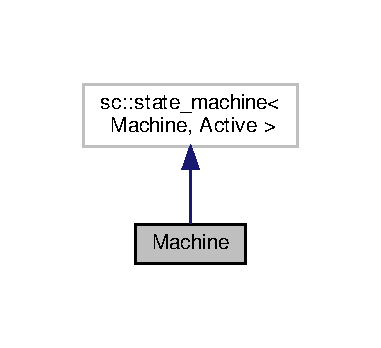
\includegraphics[width=183pt]{structMachine__inherit__graph}
\end{center}
\end{figure}


Collaboration diagram for Machine\+:
\nopagebreak
\begin{figure}[H]
\begin{center}
\leavevmode
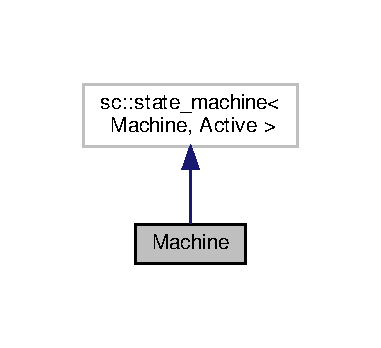
\includegraphics[width=183pt]{structMachine__coll__graph}
\end{center}
\end{figure}


The documentation for this struct was generated from the following file\+:\begin{DoxyCompactItemize}
\item 
/home/samuel/\+Desktop/toolcog\+\_\+ws/montecarlo/include/tool\+\_\+expt/\hyperlink{machine_8h}{machine.\+h}\end{DoxyCompactItemize}

\hypertarget{structManipulate}{}\section{Manipulate Struct Reference}
\label{structManipulate}\index{Manipulate@{Manipulate}}


State machine Event structure\+: Manipulation This event is invoked by Olivia state machine when in the \hyperlink{structActive}{Active} state. Perform sequences of action to manipulate object to a given target goal.  




{\ttfamily \#include $<$manipulate.\+h$>$}



Inheritance diagram for Manipulate\+:
\nopagebreak
\begin{figure}[H]
\begin{center}
\leavevmode
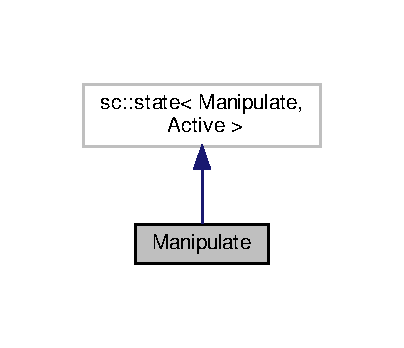
\includegraphics[width=194pt]{structManipulate__inherit__graph}
\end{center}
\end{figure}


Collaboration diagram for Manipulate\+:
\nopagebreak
\begin{figure}[H]
\begin{center}
\leavevmode
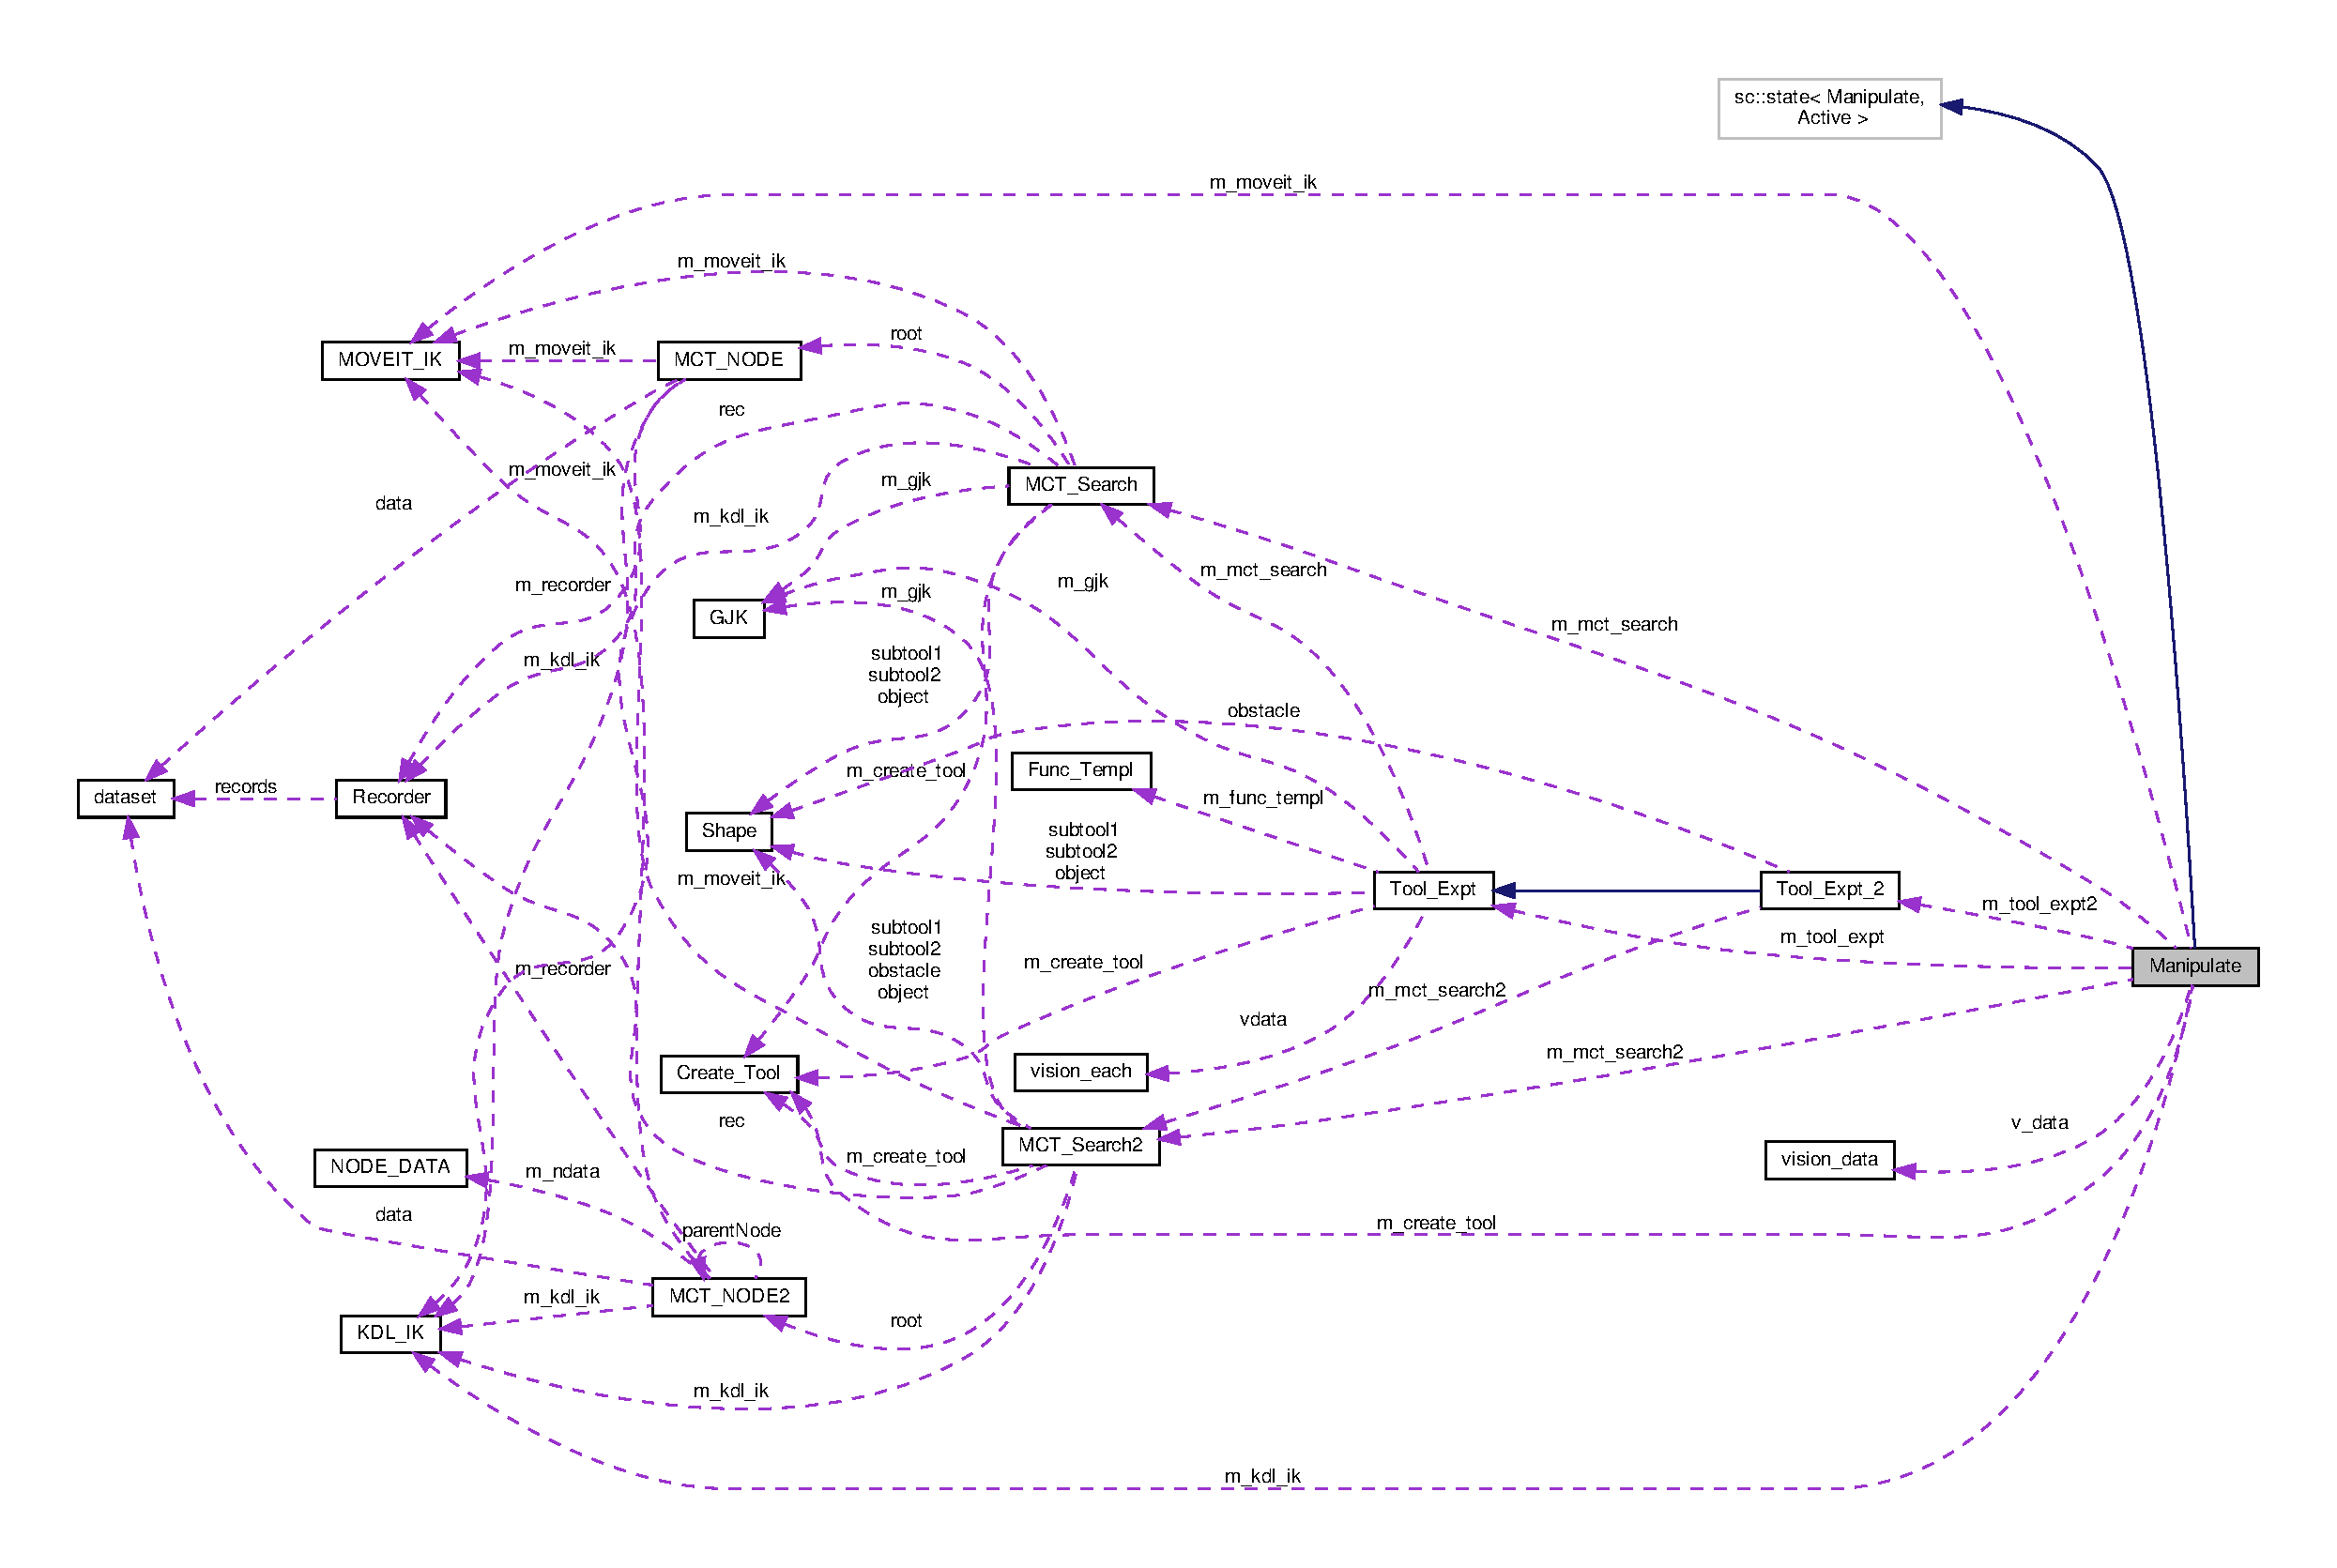
\includegraphics[width=350pt]{structManipulate__coll__graph}
\end{center}
\end{figure}
\subsection*{Public Types}
\begin{DoxyCompactItemize}
\item 
\mbox{\Hypertarget{structManipulate_a550d7f26727007d60e99c121dc3e2dd6}\label{structManipulate_a550d7f26727007d60e99c121dc3e2dd6}} 
typedef mpl\+::list$<$ sc\+::custom\+\_\+reaction$<$ \hyperlink{structEvStart}{Ev\+Start} $>$, sc\+::custom\+\_\+reaction$<$ \hyperlink{structEvPerceiveObject}{Ev\+Perceive\+Object} $>$, sc\+::custom\+\_\+reaction$<$ \hyperlink{structEvObjectFrontOfTargetRightOfRobot}{Ev\+Object\+Front\+Of\+Target\+Right\+Of\+Robot} $>$, sc\+::custom\+\_\+reaction$<$ \hyperlink{structEvObjectBackOfTargetRightOfRobot}{Ev\+Object\+Back\+Of\+Target\+Right\+Of\+Robot} $>$, sc\+::custom\+\_\+reaction$<$ \hyperlink{structEvObjectRightOfTarget}{Ev\+Object\+Right\+Of\+Target} $>$, sc\+::custom\+\_\+reaction$<$ \hyperlink{structEvObjectFrontRightOfTargetTool}{Ev\+Object\+Front\+Right\+Of\+Target\+Tool} $>$, sc\+::custom\+\_\+reaction$<$ \hyperlink{structEvObjectBackRightOfTargetTool}{Ev\+Object\+Back\+Right\+Of\+Target\+Tool} $>$, sc\+::custom\+\_\+reaction$<$ \hyperlink{structEvObjectFrontOfTargetRightOfRobotTool}{Ev\+Object\+Front\+Of\+Target\+Right\+Of\+Robot\+Tool} $>$, sc\+::custom\+\_\+reaction$<$ \hyperlink{structEvObjectFrontOfTargetLeftOfRobotTool}{Ev\+Object\+Front\+Of\+Target\+Left\+Of\+Robot\+Tool} $>$, sc\+::custom\+\_\+reaction$<$ \hyperlink{structEvObjectRightOfTargetTool}{Ev\+Object\+Right\+Of\+Target\+Tool} $>$, sc\+::custom\+\_\+reaction$<$ \hyperlink{structEvObjectBackOfTargetRightOfRobotTool}{Ev\+Object\+Back\+Of\+Target\+Right\+Of\+Robot\+Tool} $>$, sc\+::custom\+\_\+reaction$<$ \hyperlink{structEvReady}{Ev\+Ready} $>$, sc\+::custom\+\_\+reaction$<$ \hyperlink{structEvTargetNofObject}{Ev\+Target\+Nof\+Object} $>$, sc\+::custom\+\_\+reaction$<$ \hyperlink{structEvTargetSofObject}{Ev\+Target\+Sof\+Object} $>$, sc\+::custom\+\_\+reaction$<$ \hyperlink{structEvTargetOmniObject}{Ev\+Target\+Omni\+Object} $>$, sc\+::custom\+\_\+reaction$<$ \hyperlink{structEvMonteCarloExpt}{Ev\+Monte\+Carlo\+Expt} $>$, sc\+::custom\+\_\+reaction$<$ \hyperlink{structEvMonteCarloExpt2}{Ev\+Monte\+Carlo\+Expt2} $>$, sc\+::custom\+\_\+reaction$<$ \hyperlink{structEvMonteCarloExpt2__left}{Ev\+Monte\+Carlo\+Expt2\+\_\+left} $>$, sc\+::custom\+\_\+reaction$<$ \hyperlink{structEvMonteCarloExpt3__left}{Ev\+Monte\+Carlo\+Expt3\+\_\+left} $>$ $>$ \hyperlink{structManipulate_a550d7f26727007d60e99c121dc3e2dd6}{reactions}
\begin{DoxyCompactList}\small\item\em list of state machine transition reaction \end{DoxyCompactList}\end{DoxyCompactItemize}
\subsection*{Public Member Functions}
\begin{DoxyCompactItemize}
\item 
\hyperlink{structManipulate_ade8f8feaa7693b19b0038f3099218dec}{Manipulate} (my\+\_\+context ctx)
\begin{DoxyCompactList}\small\item\em Construct a new \hyperlink{structManipulate}{Manipulate} object. \end{DoxyCompactList}\item 
\mbox{\Hypertarget{structManipulate_a7f88f9adaa854ff1eb2dd02331b36f58}\label{structManipulate_a7f88f9adaa854ff1eb2dd02331b36f58}} 
\hyperlink{structManipulate_a7f88f9adaa854ff1eb2dd02331b36f58}{$\sim$\+Manipulate} ()
\begin{DoxyCompactList}\small\item\em Destroy the \hyperlink{structManipulate}{Manipulate} object. \end{DoxyCompactList}\item 
\mbox{\Hypertarget{structManipulate_a5e4d101e87c8741a40feb00fb8cde9d9}\label{structManipulate_a5e4d101e87c8741a40feb00fb8cde9d9}} 
sc\+::result {\bfseries react} (const \hyperlink{structEvStart}{Ev\+Start} \&)
\item 
\mbox{\Hypertarget{structManipulate_a1fd71a2e39bc9e69b3ddc0e6f3b5201d}\label{structManipulate_a1fd71a2e39bc9e69b3ddc0e6f3b5201d}} 
sc\+::result {\bfseries react} (const \hyperlink{structEvPerceiveObject}{Ev\+Perceive\+Object} \&)
\item 
\mbox{\Hypertarget{structManipulate_a53b0d346224cac7aa19afaec71a67a29}\label{structManipulate_a53b0d346224cac7aa19afaec71a67a29}} 
sc\+::result {\bfseries react} (const \hyperlink{structEvObjectFrontOfTargetRightOfRobot}{Ev\+Object\+Front\+Of\+Target\+Right\+Of\+Robot} \&)
\item 
\mbox{\Hypertarget{structManipulate_a8a41cdb3f91401e5a422f924873b67b0}\label{structManipulate_a8a41cdb3f91401e5a422f924873b67b0}} 
sc\+::result {\bfseries react} (const \hyperlink{structEvObjectBackOfTargetRightOfRobot}{Ev\+Object\+Back\+Of\+Target\+Right\+Of\+Robot} \&)
\item 
\mbox{\Hypertarget{structManipulate_a2c35a0ae75f83971edbba9a970450b82}\label{structManipulate_a2c35a0ae75f83971edbba9a970450b82}} 
sc\+::result {\bfseries react} (const \hyperlink{structEvObjectRightOfTarget}{Ev\+Object\+Right\+Of\+Target} \&)
\item 
\mbox{\Hypertarget{structManipulate_ac3ca97a6703e28d163c2971c932c44bb}\label{structManipulate_ac3ca97a6703e28d163c2971c932c44bb}} 
sc\+::result {\bfseries react} (const \hyperlink{structEvObjectFrontRightOfTargetTool}{Ev\+Object\+Front\+Right\+Of\+Target\+Tool} \&)
\item 
\mbox{\Hypertarget{structManipulate_a2efcf809cb1959ebd5c9954f57ee4df9}\label{structManipulate_a2efcf809cb1959ebd5c9954f57ee4df9}} 
sc\+::result {\bfseries react} (const \hyperlink{structEvObjectBackRightOfTargetTool}{Ev\+Object\+Back\+Right\+Of\+Target\+Tool} \&)
\item 
\mbox{\Hypertarget{structManipulate_a706d6ae92be6622f241ae4efb14ae2ff}\label{structManipulate_a706d6ae92be6622f241ae4efb14ae2ff}} 
sc\+::result {\bfseries react} (const \hyperlink{structEvObjectFrontOfTargetRightOfRobotTool}{Ev\+Object\+Front\+Of\+Target\+Right\+Of\+Robot\+Tool} \&)
\item 
\mbox{\Hypertarget{structManipulate_ae75ffd2328a4ec52514c32d741f0158a}\label{structManipulate_ae75ffd2328a4ec52514c32d741f0158a}} 
sc\+::result {\bfseries react} (const \hyperlink{structEvObjectFrontOfTargetLeftOfRobotTool}{Ev\+Object\+Front\+Of\+Target\+Left\+Of\+Robot\+Tool} \&)
\item 
\mbox{\Hypertarget{structManipulate_a68fa3d1012e40d8879e97d4802623d2f}\label{structManipulate_a68fa3d1012e40d8879e97d4802623d2f}} 
sc\+::result {\bfseries react} (const \hyperlink{structEvObjectRightOfTargetTool}{Ev\+Object\+Right\+Of\+Target\+Tool} \&)
\item 
\mbox{\Hypertarget{structManipulate_a6e5275c131e29c4b522d7dadfd188301}\label{structManipulate_a6e5275c131e29c4b522d7dadfd188301}} 
sc\+::result {\bfseries react} (const \hyperlink{structEvObjectBackOfTargetRightOfRobotTool}{Ev\+Object\+Back\+Of\+Target\+Right\+Of\+Robot\+Tool} \&)
\item 
\mbox{\Hypertarget{structManipulate_a632a7fc704db441217fa508b41d237aa}\label{structManipulate_a632a7fc704db441217fa508b41d237aa}} 
sc\+::result {\bfseries react} (const \hyperlink{structEvReady}{Ev\+Ready} \&)
\item 
\mbox{\Hypertarget{structManipulate_a0e2ca7e2da3fb96aa8c4da62bbf2a08c}\label{structManipulate_a0e2ca7e2da3fb96aa8c4da62bbf2a08c}} 
sc\+::result {\bfseries react} (const \hyperlink{structEvTargetNofObject}{Ev\+Target\+Nof\+Object} \&)
\item 
\mbox{\Hypertarget{structManipulate_a9a086a05e793f9e97dcdb06f7b959c1b}\label{structManipulate_a9a086a05e793f9e97dcdb06f7b959c1b}} 
sc\+::result {\bfseries react} (const \hyperlink{structEvTargetSofObject}{Ev\+Target\+Sof\+Object} \&)
\item 
\mbox{\Hypertarget{structManipulate_a89f9be39f0975cf6155dd9c2d033f8a1}\label{structManipulate_a89f9be39f0975cf6155dd9c2d033f8a1}} 
sc\+::result {\bfseries react} (const \hyperlink{structEvTargetOmniObject}{Ev\+Target\+Omni\+Object} \&)
\item 
\mbox{\Hypertarget{structManipulate_a1c5dbf4a1e7f2f450de435bfdb251a98}\label{structManipulate_a1c5dbf4a1e7f2f450de435bfdb251a98}} 
sc\+::result {\bfseries react} (const \hyperlink{structEvMonteCarloExpt}{Ev\+Monte\+Carlo\+Expt} \&)
\item 
\mbox{\Hypertarget{structManipulate_a0443f72cbf50b889a58af12edbe776ff}\label{structManipulate_a0443f72cbf50b889a58af12edbe776ff}} 
sc\+::result {\bfseries react} (const \hyperlink{structEvMonteCarloExpt2}{Ev\+Monte\+Carlo\+Expt2} \&)
\item 
\mbox{\Hypertarget{structManipulate_ae46cd1df34be565ef404c636ed018e2a}\label{structManipulate_ae46cd1df34be565ef404c636ed018e2a}} 
sc\+::result {\bfseries react} (const \hyperlink{structEvMonteCarloExpt2__left}{Ev\+Monte\+Carlo\+Expt2\+\_\+left} \&)
\item 
\mbox{\Hypertarget{structManipulate_a0bcc26e5275e2611756ee069a3832c41}\label{structManipulate_a0bcc26e5275e2611756ee069a3832c41}} 
sc\+::result {\bfseries react} (const \hyperlink{structEvMonteCarloExpt3__left}{Ev\+Monte\+Carlo\+Expt3\+\_\+left} \&)
\end{DoxyCompactItemize}
\subsection*{Private Member Functions}
\begin{DoxyCompactItemize}
\item 
void \hyperlink{structManipulate_a85f27b19ae91a8829d0864fb2a0329c2}{object\+\_\+printout\+\_\+call\+Back} (const geometry\+\_\+msgs\+::\+Pose\+Array\+::\+Ptr \&msg)
\begin{DoxyCompactList}\small\item\em subscriber callback to output object data on screen \end{DoxyCompactList}\item 
void \hyperlink{structManipulate_a7d9d1528dc39485735d019244b0a7fca}{object\+\_\+target\+\_\+positions\+\_\+call\+Back} (const geometry\+\_\+msgs\+::\+Pose\+Array\+::\+Ptr \&msg)
\begin{DoxyCompactList}\small\item\em subscriber callback to obtain target pose with respect to object from perception module \end{DoxyCompactList}\item 
void \hyperlink{structManipulate_abfa252d6d9085b184ba68156aac3d308}{tool\+\_\+handle\+\_\+position\+\_\+call\+Back} (const geometry\+\_\+msgs\+::\+Pose\+::\+Ptr \&msg)
\begin{DoxyCompactList}\small\item\em subscriber callback to obtain position of tool handle from perception module \end{DoxyCompactList}\item 
void \hyperlink{structManipulate_a0fb363bbdf2dd806b20206e32fda91ac}{bendtool\+\_\+position\+\_\+call\+Back} (const geometry\+\_\+msgs\+::\+Pose\+::\+Ptr \&msg)
\begin{DoxyCompactList}\small\item\em subscriber callback to obtain position of bendtool handle from perception module \end{DoxyCompactList}\item 
void \hyperlink{structManipulate_a6482d959b897def2c9999acaa53b191a}{fake\+\_\+tool\+\_\+transform\+\_\+call\+Back} (const geometry\+\_\+msgs\+::\+Pose\+Array\+::\+Ptr \&msg)
\begin{DoxyCompactList}\small\item\em subscriber callback to obtain tf of a fake tool \end{DoxyCompactList}\item 
void \hyperlink{structManipulate_a696de40873f30c2702d53bf9e342c1da}{fake\+\_\+target\+\_\+call\+Back} (const geometry\+\_\+msgs\+::\+Pose\+Array\+::\+Ptr \&msg)
\begin{DoxyCompactList}\small\item\em subscriber callback to obtain position of a fake target \end{DoxyCompactList}\item 
void \hyperlink{structManipulate_ab242dd492f9b8fc88564bb6583e0324a}{calib\+\_\+tool\+\_\+poses\+\_\+call\+Back} (const geometry\+\_\+msgs\+::\+Pose\+Array\+::\+Ptr \&msg)
\begin{DoxyCompactList}\small\item\em subscriber callback to calibrate tool pose \end{DoxyCompactList}\item 
void \hyperlink{structManipulate_a749da7d9cfed1b07a3aeb9f42e2258e8}{tool\+\_\+decision\+\_\+call\+Back} (const std\+\_\+msgs\+::\+Int32\+::\+Ptr \&msg)
\begin{DoxyCompactList}\small\item\em subscriber callback to obtain decision for which tool to use \end{DoxyCompactList}\item 
void \hyperlink{structManipulate_a9e3d1cc97074dbddcfe4abaa9a55425e}{calib\+\_\+next\+\_\+call\+Back} (const std\+\_\+msgs\+::\+Int32\+::\+Ptr \&msg)
\begin{DoxyCompactList}\small\item\em subscriber callback to perform calibration for next tool \end{DoxyCompactList}\item 
void \hyperlink{structManipulate_a197a10328ff64f9452a3b0be22dd8d70}{joint\+\_\+states\+\_\+call\+Back} (const sensor\+\_\+msgs\+::\+Joint\+State\+::\+Ptr \&msg)
\begin{DoxyCompactList}\small\item\em subscriber callback to obtain joint states of Olivia robot \end{DoxyCompactList}\item 
void \hyperlink{structManipulate_a4613e373fc630c6f172f8c62b0bbf6a2}{sticklength\+\_\+call\+Back} (const std\+\_\+msgs\+::\+Float64\+::\+Ptr \&msg)
\begin{DoxyCompactList}\small\item\em subscriber callback to obtain length of perceived tool/stick \end{DoxyCompactList}\item 
void \hyperlink{structManipulate_a0fd9ffe9c66fd0927721c77a6a390e67}{neck\+\_\+pan\+\_\+state\+\_\+call\+Back} (const sensor\+\_\+msgs\+::\+Joint\+State\+::\+Ptr \&msg)
\begin{DoxyCompactList}\small\item\em subscriber callback to obtain joint state of Olivia neck The neck pan motor for Olivia was separately added to allow rotation of the neck Hence, the joint state was obtained individually here \end{DoxyCompactList}\item 
m3\+\_\+moveit\+::\+Moveit\+Whole\+Body\+Goal \hyperlink{structManipulate_aaf8eadf2c5afb08213485c6bd9327fac}{fill\+Joint\+Names\+Full} ()
\begin{DoxyCompactList}\small\item\em Function to fill moveit action goal with the joint name of group used on Olivia. \end{DoxyCompactList}\item 
m3\+\_\+moveit\+::\+Moveit\+Whole\+Body\+Goal \hyperlink{structManipulate_a561688c2810b273b969b9bc8594bcac3}{fill\+Names\+Full} ()
\begin{DoxyCompactList}\small\item\em Function to fill moveit action goal with all the joint names on Olivia. \end{DoxyCompactList}\item 
m3\+\_\+moveit\+::\+Moveit\+Whole\+Body\+Goal \hyperlink{structManipulate_a1c91c2b91d2012652f62071e45899a21}{Set\+Joint\+Targets\+To\+Current} ()
\begin{DoxyCompactList}\small\item\em Set the Joint Targets To Current Position -\/$>$ used as default. \end{DoxyCompactList}\item 
Eigen\+::\+Matrix\+Xd \hyperlink{structManipulate_aadbaa24ccd292595a3821155f2bb8b99}{Compute\+Tool2\+Hand\+Transform} (const geometry\+\_\+msgs\+::\+Pose\+Array calib\+\_\+hand\+\_\+poses, const geometry\+\_\+msgs\+::\+Pose\+Array calib\+\_\+tool\+\_\+poses)
\begin{DoxyCompactList}\small\item\em Function to compute the transform matrix of Tool object to Olivia\textquotesingle{}s Hand Basically, this computes how to hold the tool in olivia\textquotesingle{}s hand. \end{DoxyCompactList}\item 
std\+::vector$<$ std\+::string $>$ \hyperlink{structManipulate_a08707bdbba233e0375b6d79b69c413da}{fill\+Joint\+Names\+Fingers} (std\+::string hand)
\begin{DoxyCompactList}\small\item\em Function to get only the joint names of the fingers in a single Olivia\textquotesingle{}s hand. \end{DoxyCompactList}\item 
std\+::vector$<$ std\+::string $>$ \hyperlink{structManipulate_a3cba926b57fd0e0ab0219b992504bd1c}{fill\+Joint\+Names\+Fingers\+Encoders} (std\+::string hand)
\begin{DoxyCompactList}\small\item\em Function to get only the joint names of the finger encoders in a single Olivia\textquotesingle{}s hand. \end{DoxyCompactList}\item 
std\+::vector$<$ geometry\+\_\+msgs\+::\+Point $>$ \hyperlink{structManipulate_a2aa3e3c677f9929cb4219b8785e1e225}{load\+\_\+boundary} (const int functionality)
\begin{DoxyCompactList}\small\item\em generate the boundary data for different hand poses The boundary data depends on the functionality that is required to be performed. Such as pushing or pulling and etc. \end{DoxyCompactList}\item 
geometry\+\_\+msgs\+::\+Pose\+Stamped \hyperlink{structManipulate_a54501e8b26698b01137421f7a20a4381}{transform\+Pose} (geometry\+\_\+msgs\+::\+Pose pose\+\_\+msg, std\+::string from\+\_\+frame, std\+::string to\+\_\+frame)
\begin{DoxyCompactList}\small\item\em Function to change a given pose from its current frame to another frame. \end{DoxyCompactList}\item 
bool \hyperlink{structManipulate_a5aaebe2cacce6f5bb4c28385ed4b85df}{is\+Reachable} (geometry\+\_\+msgs\+::\+Pose pose)
\begin{DoxyCompactList}\small\item\em Function to check if given pose is reachable by Olivia\textquotesingle{}s arm. \end{DoxyCompactList}\item 
bool \hyperlink{structManipulate_a118cc711fca21f8b4db0ef16b5e40022}{Tool\+In\+Hand\+Calibration} (std\+::string hand)
\begin{DoxyCompactList}\small\item\em Function to request a sequence of motion to calibrate the pose of the tool. \end{DoxyCompactList}\item 
\mbox{\Hypertarget{structManipulate_a6bb3429ac130fad8eb77d50151298367}\label{structManipulate_a6bb3429ac130fad8eb77d50151298367}} 
void \hyperlink{structManipulate_a6bb3429ac130fad8eb77d50151298367}{Check\+Object\+Location} ()
\begin{DoxyCompactList}\small\item\em Function to do a sweep with Olivia\textquotesingle{}s neck to detect the object\textquotesingle{}s location. \end{DoxyCompactList}\item 
\mbox{\Hypertarget{structManipulate_a3e457a70c1e1f7a5fc374981a41458d8}\label{structManipulate_a3e457a70c1e1f7a5fc374981a41458d8}} 
void \hyperlink{structManipulate_a3e457a70c1e1f7a5fc374981a41458d8}{Check\+Tool\+Location} ()
\begin{DoxyCompactList}\small\item\em Function to do a sweep with Olivia\textquotesingle{}s neck to search for viable tool. \end{DoxyCompactList}\item 
\mbox{\Hypertarget{structManipulate_aef7247c87eca27ea051a604432db97aa}\label{structManipulate_aef7247c87eca27ea051a604432db97aa}} 
void \hyperlink{structManipulate_aef7247c87eca27ea051a604432db97aa}{Check\+Bend\+Tool\+Location} ()
\begin{DoxyCompactList}\small\item\em Function to do a sweep with Olivia\textquotesingle{}s neck to search for viable bendtool. \end{DoxyCompactList}\item 
\mbox{\Hypertarget{structManipulate_a9cfc78219c5a2bac412568c51cb8ac42}\label{structManipulate_a9cfc78219c5a2bac412568c51cb8ac42}} 
void \hyperlink{structManipulate_a9cfc78219c5a2bac412568c51cb8ac42}{Check\+Fake\+Tool\+Transform} ()
\begin{DoxyCompactList}\small\item\em Function to obtain the transform matrix of a fake tool. \end{DoxyCompactList}\item 
\mbox{\Hypertarget{structManipulate_a27369858402287d0885d8acb960f967e}\label{structManipulate_a27369858402287d0885d8acb960f967e}} 
void \hyperlink{structManipulate_a27369858402287d0885d8acb960f967e}{Check\+Bend\+Tool\+Transform} ()
\begin{DoxyCompactList}\small\item\em Function to obtain the transform matrix of a bend tool. \end{DoxyCompactList}\item 
void \hyperlink{structManipulate_a1066742e96c25662bc7b8869ee3f2e9a}{Move\+Waist} (double angle\+\_\+deg)
\begin{DoxyCompactList}\small\item\em Function to call moveit to rotate the Waist to target angle. \end{DoxyCompactList}\item 
void \hyperlink{structManipulate_af8c10b24461040330efbe1d163b455f7}{Move\+Waist\+From\+Current} (double angle\+\_\+deg)
\begin{DoxyCompactList}\small\item\em Function to call moveit to rotate the Waist by an incremental angle from current. \end{DoxyCompactList}\item 
void \hyperlink{structManipulate_a4b1a50327ead8dd1414718942b36d7e6}{Move\+Waist\+Trunk\+From\+Current} (double angle\+\_\+deg, double angle\+\_\+deg\+\_\+2)
\begin{DoxyCompactList}\small\item\em Function to call moveit to move the waist \& the trunk of Olivia. There are 2 joints involved, waist and trunk. \end{DoxyCompactList}\item 
\mbox{\Hypertarget{structManipulate_ae44202238a969a4ddeee742b07576c34}\label{structManipulate_ae44202238a969a4ddeee742b07576c34}} 
void \hyperlink{structManipulate_ae44202238a969a4ddeee742b07576c34}{Reset\+Puck} ()
\begin{DoxyCompactList}\small\item\em In gazebo simulation only. Function call for gazebo to respawn Puck object. \end{DoxyCompactList}\item 
\mbox{\Hypertarget{structManipulate_ad5bff0cebc6324bfd5669d17aa4b11a1}\label{structManipulate_ad5bff0cebc6324bfd5669d17aa4b11a1}} 
void \hyperlink{structManipulate_ad5bff0cebc6324bfd5669d17aa4b11a1}{Reset\+Tool} ()
\begin{DoxyCompactList}\small\item\em In gazebo simulation only. Function call for gazebo to respawn Tool object. \end{DoxyCompactList}\item 
\mbox{\Hypertarget{structManipulate_a6917611555f9760c46d2fd9324203c37}\label{structManipulate_a6917611555f9760c46d2fd9324203c37}} 
void \hyperlink{structManipulate_a6917611555f9760c46d2fd9324203c37}{Draw\+Circle} ()
\begin{DoxyCompactList}\small\item\em Function to compute a circle. \end{DoxyCompactList}\item 
\mbox{\Hypertarget{structManipulate_a6d9060d7424ac225510e6d661ed2d8fb}\label{structManipulate_a6d9060d7424ac225510e6d661ed2d8fb}} 
void \hyperlink{structManipulate_a6d9060d7424ac225510e6d661ed2d8fb}{Test\+Hand\+Orient} ()
\begin{DoxyCompactList}\small\item\em Function call for moveit to move hand/end-\/effector to a hardcoded position. Prototype function to test moveit only. Used for maintenance/hardware debugging check. \end{DoxyCompactList}\item 
\mbox{\Hypertarget{structManipulate_ab6b6d749382344cbcfb7f93f9be8956b}\label{structManipulate_ab6b6d749382344cbcfb7f93f9be8956b}} 
void \hyperlink{structManipulate_ab6b6d749382344cbcfb7f93f9be8956b}{Home} ()
\begin{DoxyCompactList}\small\item\em Function to call moveit to send Olivia into \textquotesingle{}Home\textquotesingle{} pose. \end{DoxyCompactList}\item 
int \hyperlink{structManipulate_a565b7ca35dd49f47e2bfed2ee9157555}{Home} (double waist\+\_\+val)
\begin{DoxyCompactList}\small\item\em Function to call moveit to send Olivia into \textquotesingle{}Home\textquotesingle{} pose but at a given Waist orientation Please check moveit srdf file for joint angles of stated \textquotesingle{}Home\textquotesingle{} pose. \end{DoxyCompactList}\item 
int \hyperlink{structManipulate_a2861a353de55f324c1d8c35941417698}{Home2} (double waist\+\_\+val=0)
\begin{DoxyCompactList}\small\item\em Function to call moveit to send Olivia into \textquotesingle{}Home2\textquotesingle{} pose but at a given Waist orientation Please check moveit srdf file for joint angles of stated \textquotesingle{}Home2\textquotesingle{} pose. \end{DoxyCompactList}\item 
void \hyperlink{structManipulate_a6d5bd85cd1be15a91afc75877718de08}{Speech} (std\+::string string)
\begin{DoxyCompactList}\small\item\em Function to call speech library to vocalise a text. \end{DoxyCompactList}\item 
double \hyperlink{structManipulate_a423d2c284a0ecab7089b36908e5e871a}{signum} (const double num)
\begin{DoxyCompactList}\small\item\em return sign of number \end{DoxyCompactList}\item 
void \hyperlink{structManipulate_ad07aa34d6fcf28db6068e114acc0357b}{translate\+Hand\+From\+Current} (const std\+::string link, const std\+::vector$<$ double $>$ moveX, const std\+::vector$<$ double $>$ moveY, const std\+::vector$<$ double $>$ moveZ, const int Npts, geometry\+\_\+msgs\+::\+Pose\+Array \&pose\+\_\+array\+\_\+target)
\begin{DoxyCompactList}\small\item\em Function to move Olivia\textquotesingle{}s hand by a given amount from it\textquotesingle{}s current position. \end{DoxyCompactList}\item 
void \hyperlink{structManipulate_a2a7bcfd0f83e32f0c1e98eeef3de195b}{get\+Current\+Transforms} (tf\+::\+Quaternion \&tf\+Quat\+\_\+left, tf\+::\+Quaternion \&tf\+Quat\+\_\+right, tf\+::\+Vector3 \&tf\+Vec\+\_\+left, tf\+::\+Vector3 \&tf\+Vec\+\_\+right)
\begin{DoxyCompactList}\small\item\em Get the Current Transforms of Olivia\textquotesingle{}s left and right arm. \end{DoxyCompactList}\item 
void \hyperlink{structManipulate_ac2b42e79d4785602c5e32e6f34db0745}{get\+Current\+Transform} (const std\+::string link, tf\+::\+Quaternion \&tf\+Quat, tf\+::\+Vector3 \&tf\+Vec)
\begin{DoxyCompactList}\small\item\em Get the Current Transform of Olivia\textquotesingle{}s given link. \end{DoxyCompactList}\item 
bool \hyperlink{structManipulate_a1409babf135ae08e5957a325b2c64432}{get\+Current\+Transform} (const std\+::string link, geometry\+\_\+msgs\+::\+Pose\+Stamped \&output)
\begin{DoxyCompactList}\small\item\em Get the Current Transform of Olivia\textquotesingle{}s given link, return in geometry pose. \end{DoxyCompactList}\item 
int \hyperlink{structManipulate_a21c87a257e786f4ab336d26074770283}{Pickup\+Tool\+Right\+Arm} ()
\begin{DoxyCompactList}\small\item\em Action Sequence to pick up Tool with the right arm of Olivia. \end{DoxyCompactList}\item 
int \hyperlink{structManipulate_aba8393a0211102ece9e667969dc20102}{Pickup\+Bend\+Tool} ()
\begin{DoxyCompactList}\small\item\em Action Sequence to pick up Bend Tool -\/$>$ first test case. \end{DoxyCompactList}\item 
int \hyperlink{structManipulate_a4e119e64742c41a9c460f9a6f7dbca66}{Bend\+Tool} (double stick\+\_\+length, double head\+\_\+length, double head\+\_\+angle\+\_\+deg)
\begin{DoxyCompactList}\small\item\em Action Sequence to pick up a Bend Tool with variable length. \end{DoxyCompactList}\item 
int \hyperlink{structManipulate_a9773bc419a59c54669e7ace7b1c71860}{Open\+Fingers} (std\+::string side, int mode)
\begin{DoxyCompactList}\small\item\em Function to open the fingers of Olivia. \end{DoxyCompactList}\item 
int \hyperlink{structManipulate_ad3176a1acd09b15e80a5455b4df47515}{Close\+Fingers} (std\+::string side, int grasp\+\_\+type, int mode)
\begin{DoxyCompactList}\small\item\em Function to close fingers of Olivia. \end{DoxyCompactList}\item 
int \hyperlink{structManipulate_ad24d102e05574988b0d5410f72af55d9}{Action\+Pull\+Back\+Left\+Arm} ()
\begin{DoxyCompactList}\small\item\em Action sequence to pull back left arm. \end{DoxyCompactList}\item 
int \hyperlink{structManipulate_aad9e6bf0e8c675cdc6a516effcaca20c}{Action\+Pull\+Back\+Right\+Arm} ()
\begin{DoxyCompactList}\small\item\em Action sequence to pull back right arm. \end{DoxyCompactList}\item 
int \hyperlink{structManipulate_ae5d9a3633a709aee251e8f73126b7362}{Action\+Pull\+Back\+Right\+Arm\+Tool} ()
\begin{DoxyCompactList}\small\item\em Action sequence to pull back right arm with tool in hand. \end{DoxyCompactList}\item 
int \hyperlink{structManipulate_ab094520fdf91df726e8458724bd10eaf}{Action\+Pull\+Back\+Bend\+Tool} ()
\begin{DoxyCompactList}\small\item\em Action sequence to pull back arm with bendtool in hand. \end{DoxyCompactList}\item 
int \hyperlink{structManipulate_a0bec14a9892d05383bf8df05ce2c5890}{Action\+Push\+Sideways\+Left\+Arm} ()
\begin{DoxyCompactList}\small\item\em Action sequence to push sideways with left arm. \end{DoxyCompactList}\item 
int \hyperlink{structManipulate_a5a401d36a7b32fb608c0d432091fc3dc}{Action\+Push\+Sideways\+Right\+Arm} ()
\begin{DoxyCompactList}\small\item\em Action sequence to push sidewyas with right arm. \end{DoxyCompactList}\item 
int \hyperlink{structManipulate_aee20bd1d48720fa28e12abbe42fdef57}{Action\+Push\+Forward\+Left\+Arm} ()
\begin{DoxyCompactList}\small\item\em Action sequence to push forward left direction with left arm. \end{DoxyCompactList}\item 
int \hyperlink{structManipulate_a128e631593f945ea431116aef97a4511}{Action\+Push\+Forward\+Right\+Arm} (bool using\+\_\+tool)
\begin{DoxyCompactList}\small\item\em Action sequence to push forward with right arm. \end{DoxyCompactList}\item 
int \hyperlink{structManipulate_ac49e6b0ca61223d49110e1dbf02f086e}{Action\+Push\+Forward\+Right\+Arm\+Special} ()
\begin{DoxyCompactList}\small\item\em Action sequence to push forward right with arm. special sequence test. \end{DoxyCompactList}\item 
int \hyperlink{structManipulate_a0bd90bbdd4f24ba6740da3e789210982}{Action\+Return\+Tool\+Right\+Arm} ()
\begin{DoxyCompactList}\small\item\em Action sequence to Return Tool back to where it was obtained. For right arm. \end{DoxyCompactList}\item 
int \hyperlink{structManipulate_a0ce9ec47f0cf4f42cdf0dfcf29387ebb}{Action\+Return\+Tool\+Right\+Arm\+Special} ()
\begin{DoxyCompactList}\small\item\em Action sequence to Return Tool back to where it was obtained. For right arm, special sequence test. \end{DoxyCompactList}\item 
int \hyperlink{structManipulate_a2a2cd9af2803118298b33008c27a295d}{Action\+Return\+Bend\+Tool} ()
\begin{DoxyCompactList}\small\item\em Action sequence to Return Bend\+Tool back to where it was obtained. \end{DoxyCompactList}\item 
int \hyperlink{structManipulate_a187b5b722ac34bb0718478120b0a4262}{Action\+Push\+ForwardN} ()
\begin{DoxyCompactList}\small\item\em Action sequence to push forward in North direction. \end{DoxyCompactList}\item 
int \hyperlink{structManipulate_a2ea0628e45e9350185fb172819448256}{Action\+Push\+Forward\+N\+\_\+\+Tool} ()
\begin{DoxyCompactList}\small\item\em Action sequence to push forward in North direction with tool. \end{DoxyCompactList}\item 
int \hyperlink{structManipulate_a1caf8c447479cbcdc346b0959bd5100f}{Action\+PushbackS} ()
\begin{DoxyCompactList}\small\item\em Action sequence to pull object towards south direction. \end{DoxyCompactList}\item 
int \hyperlink{structManipulate_a93385c3e5e0efd1524cde27fccfb6097}{Action\+Pushback\+S\+\_\+\+Tool} ()
\begin{DoxyCompactList}\small\item\em Action sequence to pull object towards south direction with tool. \end{DoxyCompactList}\item 
int \hyperlink{structManipulate_a4fb5a32e372f7fcfb127acf9d5bb1456}{Action\+Omni\+Right} ()
\begin{DoxyCompactList}\small\item\em Action sequence to pull/push object in any direction with right arm. \end{DoxyCompactList}\item 
int \hyperlink{structManipulate_a001314f9820e91f705a9e4e9ade17533}{Action\+Omni\+Right\+\_\+\+Tool} ()
\begin{DoxyCompactList}\small\item\em Action sequence to pull/push object in any direction with Tool in right arm. \end{DoxyCompactList}\item 
int \hyperlink{structManipulate_a43cab2081e19d5502c1cfc4265a7c9fc}{Ex\+North} ()
\begin{DoxyCompactList}\small\item\em Execution Handler function for call action sequence for North push. \end{DoxyCompactList}\item 
int \hyperlink{structManipulate_afdf5f6d0d34bff3fdfa2f3a2e590ca7f}{Ex\+North\+Tool} (bool object\+\_\+within\+\_\+reach, bool target\+\_\+within\+\_\+reach)
\begin{DoxyCompactList}\small\item\em Execution Handler function for call action sequence for North push This one also checks for target within reach or not. Decides if tool is required and what action to take. \end{DoxyCompactList}\item 
int \hyperlink{structManipulate_a3cc03e07441e7993cfa52d730196ac98}{Ex\+South} ()
\begin{DoxyCompactList}\small\item\em Execution Handler function for call action sequence for South pull. \end{DoxyCompactList}\item 
int \hyperlink{structManipulate_a0fa003e72a0b1a6bccf2658ebf49d3af}{Ex\+South\+Tool} (bool object\+\_\+within\+\_\+reach, bool target\+\_\+within\+\_\+reach)
\begin{DoxyCompactList}\small\item\em Execution Handler function for call action sequence for South pull This one also checks for target within reach or not. Decides if tool is required and what action to take. \end{DoxyCompactList}\item 
int \hyperlink{structManipulate_ad8c0f3dc7de79a53da885f538354cfd8}{Ex\+Omni} (bool repoflag)
\begin{DoxyCompactList}\small\item\em Execution Handler function for call action sequence for omnidirectional pull/push. \end{DoxyCompactList}\item 
int \hyperlink{structManipulate_a5878c899118b3be92224c4b276ae06ff}{Ex\+Omni\+Tool} (bool object\+\_\+within\+\_\+reach, bool target\+\_\+within\+\_\+reach)
\begin{DoxyCompactList}\small\item\em Execution Handler function for call action sequence for omnidirectional pull/push This one also checks for target within reach or not. Decides if tool is required and what action to take. \end{DoxyCompactList}\item 
int \hyperlink{structManipulate_a74fb07d3b191e25ca23c36b1cc7ed6a9}{pinch\+Fingers} (std\+::string side, double diameter\+\_\+in\+\_\+cm, int mode)
\begin{DoxyCompactList}\small\item\em Function to perform pinching with Olivia fingers Compute the encoder value to close based on input tool size. \end{DoxyCompactList}\item 
int \hyperlink{structManipulate_ac16ad710b70a15624c7952b35a891974}{power\+Fingers} (std\+::string side, double diameter\+\_\+in\+\_\+cm, int mode)
\begin{DoxyCompactList}\small\item\em Function to perform pinching with Olivia fingers but with tighter grip force Compute the encoder value to close based on input tool size but tighter (larger gain) \end{DoxyCompactList}\item 
int \hyperlink{structManipulate_a7e87b30f595ed31297fcd2e8759b6fb1}{Move\+Fingers} (std\+::string side, double fraction, int mode)
\begin{DoxyCompactList}\small\item\em Function to move fingers based on fraction between minimum and maximum joint values. \end{DoxyCompactList}\item 
int \hyperlink{structManipulate_a51974f3f0cfc09d119d229b7a3386d24}{Neck\+Tilt} (double neck\+\_\+tilt\+\_\+angle)
\begin{DoxyCompactList}\small\item\em Function to tilt neck to desired angle. \end{DoxyCompactList}\item 
int \hyperlink{structManipulate_ad830a25f512992ea9629b49763ea72a7}{Neck\+Pan} (double pan\+\_\+angle, double pan\+\_\+speed)
\begin{DoxyCompactList}\small\item\em Function to pan the neck to desired angle. \end{DoxyCompactList}\item 
int \hyperlink{structManipulate_aad305b9b5bc679d1c13754bdd8c73127}{Turn\+Head\+To\+Obj\+Tar\+Center} ()
\begin{DoxyCompactList}\small\item\em Funtion to compute what angle to turn the neck to face the detected object center. \end{DoxyCompactList}\item 
int \hyperlink{structManipulate_a32c081d7276be31a467cde4ab4e9c9e3}{Turn\+Head\+Tilt\+Pan} (double neck\+\_\+tilt\+\_\+angle, double neck\+\_\+pan\+\_\+angle)
\begin{DoxyCompactList}\small\item\em Function to perform both neck panning and tilting at the same time. \end{DoxyCompactList}\item 
void \hyperlink{structManipulate_a0611b33a34a32092d6265b06e4074d73}{Action\+Client\+Neck\+Pan\+Done\+Callback} (const actionlib\+::\+Simple\+Client\+Goal\+State \&state, const neck\+\_\+pan\+::\+Neck\+Pan\+Result\+Const\+Ptr \&result)
\begin{DoxyCompactList}\small\item\em Action sequence to perform both neck pan and tilt. \end{DoxyCompactList}\item 
double \hyperlink{structManipulate_a2e95c0cd30bc9c8a3d712d681d70ab3d}{compute\+\_\+min\+\_\+aug} (const std\+::vector$<$ geometry\+\_\+msgs\+::\+Point $>$ boundary, const geometry\+\_\+msgs\+::\+Point object, const geometry\+\_\+msgs\+::\+Point target, const bool object\+\_\+within\+\_\+reach, const bool target\+\_\+within\+\_\+reach)
\begin{DoxyCompactList}\small\item\em Function to compute the minimum augmentation required for object to reach target Augmentation length refers to the length of the tool required to push object to the target. Need to search for tool of this length. \end{DoxyCompactList}\item 
bool \hyperlink{structManipulate_a404bf3531c8b6368c0b317062b3c30e4}{kbhit} ()
\begin{DoxyCompactList}\small\item\em Keyboard input function. \end{DoxyCompactList}\item 
\mbox{\Hypertarget{structManipulate_a56344962ac193cd9ce322cc0ddf23bac}\label{structManipulate_a56344962ac193cd9ce322cc0ddf23bac}} 
Affine3d {\bfseries create\+\_\+affine} (double roll, double pitch, double yaw, double x, double y, double z)
\item 
\mbox{\Hypertarget{structManipulate_a11c5db5c7372d890fa77fae1fc1c6054}\label{structManipulate_a11c5db5c7372d890fa77fae1fc1c6054}} 
Affine3d {\bfseries create\+\_\+affine} (double roll, double pitch, double yaw, Vector3d xyz)
\item 
int \hyperlink{structManipulate_aa8b1c587db98b761dffdcc34a2a2b03c}{find\+Object\+Target\+Location} ()
\begin{DoxyCompactList}\small\item\em Obtain object and target position. \end{DoxyCompactList}\item 
int \hyperlink{structManipulate_aedf7650241c029dd3007e8744796891a}{find\+Tool\+Target\+Location} ()
\begin{DoxyCompactList}\small\item\em Obtain Tool and target position. \end{DoxyCompactList}\item 
int \hyperlink{structManipulate_a0ccd3cd41e0cb39485fe962393e69efd}{mct\+\_\+tool\+\_\+experiment} ()
\begin{DoxyCompactList}\small\item\em perform mct search and tool usage experiment This function performs the computation and planning \end{DoxyCompactList}\item 
int \hyperlink{structManipulate_ae182e793c8a517ba6ff8c2f627dffa43}{perform\+\_\+experiment} ()
\begin{DoxyCompactList}\small\item\em perform experiment This function performs the execution of the Olivia robot. Followed after solution is found by \hyperlink{structManipulate_a0ccd3cd41e0cb39485fe962393e69efd}{mct\+\_\+tool\+\_\+experiment()} function. \end{DoxyCompactList}\item 
void \hyperlink{structManipulate_a159148c2a60da01c497c2a4fe4e76e42}{done\+Cb} (const actionlib\+::\+Simple\+Client\+Goal\+State \&state, const m3\+\_\+moveit\+::\+Moveit\+Single\+Result\+Const\+Ptr \&result)
\begin{DoxyCompactList}\small\item\em Action client result callback. Non-\/blocking implementation of action client. \end{DoxyCompactList}\item 
\mbox{\Hypertarget{structManipulate_abccb09b1132e0896d6f3825e166fd241}\label{structManipulate_abccb09b1132e0896d6f3825e166fd241}} 
void \hyperlink{structManipulate_abccb09b1132e0896d6f3825e166fd241}{active\+Cb} ()
\begin{DoxyCompactList}\small\item\em Action client active callback. Non-\/blocking implementation of action client. Not used. \end{DoxyCompactList}\item 
void \hyperlink{structManipulate_aea788f083af31cad6f9519ffa5903d58}{feedback\+Cb} (const m3\+\_\+moveit\+::\+Moveit\+Single\+Feedback\+Const\+Ptr \&feedback)
\begin{DoxyCompactList}\small\item\em Action client feedback callback. Non-\/blocking implementation of action client. \end{DoxyCompactList}\item 
int \hyperlink{structManipulate_a581e8cd0fc68f7191da0a46bc888d5c6}{check\+User\+Input} ()
\begin{DoxyCompactList}\small\item\em Check for user input. When moveit planning is done, for dangerously long objects/tool, user is required to provide an input to continue with execution. \end{DoxyCompactList}\item 
int \hyperlink{structManipulate_a078e4f4dd5e337e937fb502d8b8d4fc9}{Action\+Attach\+Obj} (string arm\+\_\+name, string obj\+\_\+name, moveit\+\_\+msgs\+::\+Collision\+Object cobj)
\begin{DoxyCompactList}\small\item\em Moveit Action client call to attach a collision object to the given arm in the robot model in the planning scene for collision-\/free planning. \end{DoxyCompactList}\item 
int \hyperlink{structManipulate_ac90a0b245db67e17d0b11692b200c531}{Action\+Detach\+Obj} (string arm\+\_\+name, string obj\+\_\+name)
\begin{DoxyCompactList}\small\item\em Moveit Action Client to detact a previously attached object from the given arm. \end{DoxyCompactList}\item 
int \hyperlink{structManipulate_a5d17ffae09965e37c79af214bdcc99fd}{Action\+Rm\+Obj} (string obj\+\_\+id)
\begin{DoxyCompactList}\small\item\em Moveit Action Client to remove an object from the planning scene. \end{DoxyCompactList}\item 
int \hyperlink{structManipulate_a56189f1ea0370b1e8d680afe6cd886ea}{Action\+Add\+Obj} (string obj\+\_\+id, moveit\+\_\+msgs\+::\+Collision\+Object cobj)
\begin{DoxyCompactList}\small\item\em Moveit Action Client to add an object into the planning scene. \end{DoxyCompactList}\item 
int \hyperlink{structManipulate_a71a541174e9e4c83d1c7786a12ed19c4}{Action\+Go\+To\+Pos} ()
\begin{DoxyCompactList}\small\item\em Action to go to a position. Old test function. \end{DoxyCompactList}\item 
int \hyperlink{structManipulate_a27ddd517fdecd8eadd65d0b34efca2d1}{Action\+Go\+To\+Pos} (Affine3d this\+\_\+pose, bool plan\+\_\+only=false, string action\+\_\+name=\char`\"{}task\+\_\+single\+\_\+right\char`\"{}, bool replan=false, string link\+\_\+name=\char`\"{}ee\char`\"{})
\begin{DoxyCompactList}\small\item\em Action to go to a position. \end{DoxyCompactList}\item 
int \hyperlink{structManipulate_a73591582a036d5bfd1891b27b375ace4}{Action\+Go\+To\+Pos} (std\+::vector$<$ Affine3d $>$ these\+\_\+poses, bool plan\+\_\+only=false, string action\+\_\+name=\char`\"{}task\+\_\+single\+\_\+right\char`\"{}, bool replan=false, string link\+\_\+name=\char`\"{}ee\char`\"{})
\begin{DoxyCompactList}\small\item\em Action to go to a position via multiple waypoints. \end{DoxyCompactList}\item 
int \hyperlink{structManipulate_a6ceaa1e96d861f3d8f01d5b16dfbafca}{Action\+Go\+To\+Pos} (Vector3d action\+\_\+pos, Quaterniond action\+\_\+quat, bool plan\+\_\+only=false, string action\+\_\+name=\char`\"{}cart\+\_\+single\+\_\+right\char`\"{}, bool replan=false, string link\+\_\+name=\char`\"{}ee\char`\"{})
\begin{DoxyCompactList}\small\item\em Action to go to a position. \end{DoxyCompactList}\item 
int \hyperlink{structManipulate_a65a8f830ad439fbc5236bd6d6be2f4d8}{Action\+Go\+To\+Pos} (std\+::vector$<$ Affine3d $>$ these\+\_\+poses, double $\ast$fraction, bool plan\+\_\+only=false, string action\+\_\+name=\char`\"{}cart\+\_\+single\+\_\+right\char`\"{}, bool replan=false, string link\+\_\+name=\char`\"{}ee\char`\"{})
\begin{DoxyCompactList}\small\item\em Action to go to a position. Caertesian space planning of moveit is able to execute a plan that is not 100\% successfully planned. If planning $>$ desired fraction, execute the incomplete plan anyway. \end{DoxyCompactList}\item 
int \hyperlink{structManipulate_a76fc2b66b3fbdacf43cb31cf5ae3c2e4}{add\+Collision} (vector$<$ string $>$ ids, vector$<$ string $>$ meshfiles, vector$<$ geometry\+\_\+msgs\+::\+Pose $>$ poses)
\begin{DoxyCompactList}\small\item\em Action to add collision object into planning scene Used at prototyping stage to add known objects into the planning scene. Such as table or chair and etc. \end{DoxyCompactList}\item 
int \hyperlink{structManipulate_a74221cc0607aabde800bb0a1f5c3e67d}{add\+Tool\+Collision} ()
\begin{DoxyCompactList}\small\item\em Action to add tool collision into planning scene. Only used during gazebo simulation. \end{DoxyCompactList}\item 
int \hyperlink{structManipulate_adeeb6f85db89cf573e22bcb73c806c70}{add\+Puck\+Collision} (double radius=0.\+04)
\begin{DoxyCompactList}\small\item\em Action to add a puck collision into planning scene. Only used during gazebo simulation. \end{DoxyCompactList}\item 
int \hyperlink{structManipulate_a1f4484286205d02906a0f8d0d1d50ba5}{add\+Table\+Collision} ()
\begin{DoxyCompactList}\small\item\em Action to add a table collision into planning scene. \end{DoxyCompactList}\item 
int \hyperlink{structManipulate_a33209024eebea398fd7e81c493e0a049}{add\+Rack\+Collision} ()
\begin{DoxyCompactList}\small\item\em Action to add a tool rack collision into planning scene. \end{DoxyCompactList}\item 
Affine3d \hyperlink{structManipulate_a64a241674c3181908c7229fba21bd69b}{Estimate\+Pose} (double fraction, Affine3d start, Affine3d end)
\begin{DoxyCompactList}\small\item\em Computation function to provide pose based on interpolation When using Caertesian space planning of moveit, and planning is not 100\% to target, do this to quickly obtain a good estimate of pose before execution. \end{DoxyCompactList}\item 
bool \hyperlink{structManipulate_a64486e6e73ae0c3b64a2baf6a26a6e03}{Re\+Adjustment} (int idx, vector$<$ Affine3d $>$ gohere, double fraction, Affine3d start\+\_\+\+TF, Affine3d end\+\_\+\+TF)
\begin{DoxyCompactList}\small\item\em Compute if Re-\/adjustment is required. Usually used when moveit failed to compute a plan and need to shift the hand slightly, in hopes of allowing planning of higher success rate. \end{DoxyCompactList}\item 
int \hyperlink{structManipulate_a27f72bbd1c909b5fc1c06e320467a947}{vision\+\_\+cb\+\_\+test} ()
\begin{DoxyCompactList}\small\item\em Execution Function for perception module. \end{DoxyCompactList}\item 
void \hyperlink{structManipulate_ace713e3e91e90d051730ad0f98fc5126}{finish\+\_\+v} (bool tool\+\_\+in\+\_\+hand, bool okay=true, bool wflag=false)
\begin{DoxyCompactList}\small\item\em Action sequence to finish experiment when using perception module Return tool to rack and etc. \end{DoxyCompactList}\item 
void \hyperlink{structManipulate_ae32c3e2815aae04cc22224eddfa61078}{vision\+\_\+data\+\_\+call\+Back} (const findtoolontalbe\+::vision\+\_\+msgs\+::\+Ptr \&msg)
\begin{DoxyCompactList}\small\item\em Callback function to receive data from perception module. \end{DoxyCompactList}\item 
int \hyperlink{structManipulate_a39959395c5ee7d305eb9f1a306166abb}{add\+Visual\+Tool\+Collision} (shape\+\_\+msgs\+::\+Mesh co\+\_\+mesh)
\begin{DoxyCompactList}\small\item\em Function to add Perceived object from perception module into the moveit planning scene. \end{DoxyCompactList}\item 
int \hyperlink{structManipulate_a9d9985f555d6eae5ed7baa77fe8b0969}{display\+\_\+poses\+\_\+matrix} ()
\begin{DoxyCompactList}\small\item\em Display function to print out computed poses. For debugging check. \end{DoxyCompactList}\item 
int \hyperlink{structManipulate_a4933228a7e9745630d8a4e529bdc2e98}{display\+\_\+tool\+\_\+matrix} ()
\begin{DoxyCompactList}\small\item\em Display function to print out perceived tool matrix. \end{DoxyCompactList}\item 
int \hyperlink{structManipulate_aa62490b6991acbd41e7bcefe76523374}{return\+Tool} ()
\begin{DoxyCompactList}\small\item\em Action sequences to return Tool to where it was obtained. \end{DoxyCompactList}\item 
int \hyperlink{structManipulate_a51cda8e5d51dad3a8b7a75484e803bd8}{Action\+Switch\+TF} (int num)
\begin{DoxyCompactList}\small\item\em this is used to switch tf frames between cameras This switches between frames of olivia eyes, overhead camera for table, and a camera that looks at the tool rack. Significantly reduce effort and time required for experiment to scan and search for objects/tools/obstacles on table/rack \end{DoxyCompactList}\item 
void \hyperlink{structManipulate_aec1aa248a881c3f2c7c42d2a33f064ed}{Add\+Marker} (Affine3d pose, string name)
\begin{DoxyCompactList}\small\item\em Function to add markers to R\+V\+IZ to provide visual aids. \end{DoxyCompactList}\item 
\mbox{\Hypertarget{structManipulate_a71a59840948b21a66265da53b09bf94d}\label{structManipulate_a71a59840948b21a66265da53b09bf94d}} 
void \hyperlink{structManipulate_a71a59840948b21a66265da53b09bf94d}{publish\+Marker} ()
\begin{DoxyCompactList}\small\item\em publish all the markers to rviz \end{DoxyCompactList}\item 
\mbox{\Hypertarget{structManipulate_a292ee17af26baa74c5e91cdb94f217e9}\label{structManipulate_a292ee17af26baa74c5e91cdb94f217e9}} 
void \hyperlink{structManipulate_a292ee17af26baa74c5e91cdb94f217e9}{clear\+Marker} ()
\begin{DoxyCompactList}\small\item\em remove all the markers from rviz \end{DoxyCompactList}\item 
\mbox{\Hypertarget{structManipulate_a64ee2e12c6bc8d8a092802666f7064d3}\label{structManipulate_a64ee2e12c6bc8d8a092802666f7064d3}} 
void \hyperlink{structManipulate_a64ee2e12c6bc8d8a092802666f7064d3}{Reset\+Obstacle} ()
\begin{DoxyCompactList}\small\item\em Function to respawn obstacle in Gazebo simulation only. \end{DoxyCompactList}\item 
int \hyperlink{structManipulate_ad8cb006920541e0c78775571f62c8ce1}{add\+Obstacle\+Collision} (double radius=0.\+04)
\begin{DoxyCompactList}\small\item\em Function to add obstacle and collision into planning scene. \end{DoxyCompactList}\item 
int \hyperlink{structManipulate_a1ccca6fcd1ad2ac9d48a112cbb90fdf9}{find\+Object\+Target\+Location2} ()
\begin{DoxyCompactList}\small\item\em Updated function to detect object and target with overhead camera. \end{DoxyCompactList}\item 
int \hyperlink{structManipulate_a9f8d8093a4a0d0adf0a00148673f5781}{find\+Tool\+Target\+Location2} ()
\begin{DoxyCompactList}\small\item\em Updated function to detect tool and target location with camera looking at tool rack. \end{DoxyCompactList}\item 
int \hyperlink{structManipulate_ad42c5cd9aaae7a12c0056fe4d78fcbf8}{mct\+\_\+tool\+\_\+experiment2} ()
\begin{DoxyCompactList}\small\item\em Experiment 2 for mcts with tool Added an overhead camera for table, and a camera that looks at the tool rack. Significantly reduce effort and time required for experiment to scan and search for objects/tools/obstacles on table/rack. An improvement from just depending on Olivia\textquotesingle{}s eyes alone. \end{DoxyCompactList}\item 
int \hyperlink{structManipulate_aabfbcf8aba7c38776bc37db8d01508d6}{perform\+\_\+experiment2} ()
\begin{DoxyCompactList}\small\item\em Function to execute plan if mcts solution is successfully found. \end{DoxyCompactList}\item 
int \hyperlink{structManipulate_aff548e55e9bbfb49459a8b9b419b4dbe}{display\+\_\+poses\+\_\+matrix2} ()
\begin{DoxyCompactList}\small\item\em Display more information. \end{DoxyCompactList}\item 
int \hyperlink{structManipulate_aeb62b4d4b898f5a403e75ada463bbeb4}{find\+Tool\+Target\+Location3} ()
\begin{DoxyCompactList}\small\item\em Updated function from updated perception module data format. \end{DoxyCompactList}\item 
int \hyperlink{structManipulate_a49b4ba7bd0c11a5abe4dcfc3f0f7af0e}{mcts\+\_\+demo\+\_\+2} ()
\begin{DoxyCompactList}\small\item\em Function to perform mcts demo with updated functions. \end{DoxyCompactList}\item 
int \hyperlink{structManipulate_a4496399bd56cc674257ab8a44c991647}{write2file} ()
\begin{DoxyCompactList}\small\item\em Function to export out all the data to csv file. \end{DoxyCompactList}\item 
int \hyperlink{structManipulate_a8763018283f744613d7d50e6e22a27cf}{find\+Object\+Target\+Location2\+\_\+left} ()
\begin{DoxyCompactList}\small\item\em Function to find object and target location on the left side of olivia. \end{DoxyCompactList}\item 
int \hyperlink{structManipulate_a11da86aa5653ed4e4ddf1fe25a169a7a}{mct\+\_\+tool\+\_\+experiment2\+\_\+left} ()
\begin{DoxyCompactList}\small\item\em Function to perform the mcts demo but on the reverse left side. \end{DoxyCompactList}\item 
int \hyperlink{structManipulate_aa5bc40657d99cd3c92804a61925327cc}{perform\+\_\+experiment2\+\_\+left} ()
\begin{DoxyCompactList}\small\item\em Function to execute plan if mcts solution is successfully found. For left side and left arm. \end{DoxyCompactList}\item 
void \hyperlink{structManipulate_adedede8a7878a8065000f4bfff72b3b8}{finish\+\_\+v\+\_\+l} (bool tool\+\_\+in\+\_\+hand, bool okay=true, bool wflag=false)
\begin{DoxyCompactList}\small\item\em Action sequence to finish experiment when using perception module Return tool to rack and etc. Left side and left arm. \end{DoxyCompactList}\item 
int \hyperlink{structManipulate_a7b8394f3cd61252c79d9c1956e7aab2e}{mct\+\_\+tool\+\_\+experiment3\+\_\+left} ()
\begin{DoxyCompactList}\small\item\em M\+C\+TS experiment version3 with addition of obstacles. For left side and left arm. \end{DoxyCompactList}\item 
\mbox{\Hypertarget{structManipulate_a9a93d24747a3e47c149914d52f533849}\label{structManipulate_a9a93d24747a3e47c149914d52f533849}} 
int {\bfseries go\+Into\+Diff\+Pos} (double H\+E\+A\+D\+\_\+\+S\+I\+ZE, double H\+A\+N\+D\+L\+E\+\_\+\+L\+E\+N\+G\+TH, double H\+E\+I\+G\+H\+T\+\_\+\+L\+E\+N\+G\+TH)
\item 
\mbox{\Hypertarget{structManipulate_a8de35e42067ef7574846cd86553ac463}\label{structManipulate_a8de35e42067ef7574846cd86553ac463}} 
int {\bfseries recursive\+Pos} (double H\+E\+A\+D\+\_\+\+S\+I\+ZE, double H\+A\+N\+D\+L\+E\+\_\+\+L\+E\+N\+G\+TH, double H\+E\+I\+G\+H\+T\+\_\+\+L\+E\+N\+G\+TH)
\item 
int \hyperlink{structManipulate_a625fa2cac7d57ccc2e547461faf0a6e0}{find\+Tool\+Loca} ()
\begin{DoxyCompactList}\small\item\em Function to obtain tool pose. \end{DoxyCompactList}\item 
int \hyperlink{structManipulate_ab9223a95d1d58d8b809d82d282ce48a8}{neck\+\_\+and\+\_\+waist\+\_\+trunk} (double tilt\+\_\+angle, double pan\+\_\+angle, double pan\+\_\+speed, double angle\+\_\+deg, double angle\+\_\+deg\+\_\+2)
\begin{DoxyCompactList}\small\item\em Action function to move Olivia neck, waist and trunk at same time to desired values. \end{DoxyCompactList}\item 
bool \hyperlink{structManipulate_aaf55e7ba44c974f70ac925898c267e6c}{Ev\+Reachable} (bool P\+I\+C\+K\+\_\+\+F\+L\+AG)
\begin{DoxyCompactList}\small\item\em Function to check if object is reachable. If using robot arm to perform Pick And Place task, computation changes to detect if graspable. \end{DoxyCompactList}\item 
bool \hyperlink{structManipulate_ad31d1bed54184f5eb6caebc909390272}{Ev\+Reachable2} ()
\begin{DoxyCompactList}\small\item\em Updated function to check if object is reachable. \end{DoxyCompactList}\item 
{\footnotesize template$<$typename \+\_\+\+Matrix\+\_\+\+Type\+\_\+ $>$ }\\\+\_\+\+Matrix\+\_\+\+Type\+\_\+ \hyperlink{structManipulate_adcb737b1bd9ea1a621a668b09af275fb}{pseudo\+Inverse} (const \+\_\+\+Matrix\+\_\+\+Type\+\_\+ \&a, double epsilon=std\+::numeric\+\_\+limits$<$ double $>$\+::epsilon())
\begin{DoxyCompactList}\small\item\em compute the pseudo inverse of given matrix \end{DoxyCompactList}\end{DoxyCompactItemize}
\subsection*{Private Attributes}
\begin{DoxyCompactItemize}
\item 
\mbox{\Hypertarget{structManipulate_abd8097dcac062850c589c0154d2ae9ba}\label{structManipulate_abd8097dcac062850c589c0154d2ae9ba}} 
ros\+::\+Node\+Handle {\bfseries n}
\item 
\mbox{\Hypertarget{structManipulate_ac510ae0f52da37bc5729b428e18e0656}\label{structManipulate_ac510ae0f52da37bc5729b428e18e0656}} 
sound\+\_\+play\+::\+Sound\+Client {\bfseries speech}
\item 
\mbox{\Hypertarget{structManipulate_a213216a189b0b1993ff3d44b9f286a18}\label{structManipulate_a213216a189b0b1993ff3d44b9f286a18}} 
ros\+::\+Subscriber {\bfseries sub\+\_\+object\+\_\+printout}
\item 
\mbox{\Hypertarget{structManipulate_a7821cdd6a833ec54caf82696ce2667e3}\label{structManipulate_a7821cdd6a833ec54caf82696ce2667e3}} 
ros\+::\+Subscriber {\bfseries sub\+\_\+object}
\item 
\mbox{\Hypertarget{structManipulate_a89ce4416de1cd596e198536b398e2997}\label{structManipulate_a89ce4416de1cd596e198536b398e2997}} 
ros\+::\+Subscriber {\bfseries sub\+\_\+tool\+\_\+handle}
\item 
\mbox{\Hypertarget{structManipulate_a7f5cf48ae3e9aa4ccd6b871a95fc33b6}\label{structManipulate_a7f5cf48ae3e9aa4ccd6b871a95fc33b6}} 
ros\+::\+Subscriber {\bfseries sub\+\_\+bendtool}
\item 
\mbox{\Hypertarget{structManipulate_ac0907a45a1fcec51816e90413edd4df5}\label{structManipulate_ac0907a45a1fcec51816e90413edd4df5}} 
ros\+::\+Subscriber {\bfseries sub\+\_\+tool\+\_\+in\+\_\+hand}
\item 
\mbox{\Hypertarget{structManipulate_acf6aecf64301f96da22156ed1b3ede58}\label{structManipulate_acf6aecf64301f96da22156ed1b3ede58}} 
ros\+::\+Subscriber {\bfseries sub\+\_\+fake\+\_\+tool\+\_\+transform}
\item 
\mbox{\Hypertarget{structManipulate_a7646b18fb57daa6675d3da3d0b05284c}\label{structManipulate_a7646b18fb57daa6675d3da3d0b05284c}} 
ros\+::\+Subscriber {\bfseries sub\+\_\+fake\+\_\+target}
\item 
\mbox{\Hypertarget{structManipulate_a77e54004b68462602fb4043b31f9fbf3}\label{structManipulate_a77e54004b68462602fb4043b31f9fbf3}} 
ros\+::\+Subscriber {\bfseries sub\+\_\+calib\+\_\+next}
\item 
\mbox{\Hypertarget{structManipulate_a4c59a24c1a111a405a23a251b80d1f7d}\label{structManipulate_a4c59a24c1a111a405a23a251b80d1f7d}} 
ros\+::\+Subscriber {\bfseries sub\+\_\+calib\+\_\+tool\+\_\+poses}
\item 
\mbox{\Hypertarget{structManipulate_af670e455aec7e6ef5c39ea1377e6cafb}\label{structManipulate_af670e455aec7e6ef5c39ea1377e6cafb}} 
ros\+::\+Subscriber {\bfseries sub\+\_\+tool\+\_\+decision}
\item 
\mbox{\Hypertarget{structManipulate_ab0d061cb3ffbee5c2dedf25fa2f051c3}\label{structManipulate_ab0d061cb3ffbee5c2dedf25fa2f051c3}} 
ros\+::\+Subscriber {\bfseries sub\+\_\+joint\+\_\+states}
\item 
\mbox{\Hypertarget{structManipulate_a04dccd769426f2e7fcf1853a405566bd}\label{structManipulate_a04dccd769426f2e7fcf1853a405566bd}} 
ros\+::\+Subscriber {\bfseries sub\+\_\+sticklength}
\item 
\mbox{\Hypertarget{structManipulate_a55ff2774266be06c06325057e8896332}\label{structManipulate_a55ff2774266be06c06325057e8896332}} 
ros\+::\+Subscriber {\bfseries sub\+\_\+neck\+\_\+pan}
\item 
\mbox{\Hypertarget{structManipulate_a3a84cb51c03ce67d92c061789c88339e}\label{structManipulate_a3a84cb51c03ce67d92c061789c88339e}} 
ros\+::\+Publisher {\bfseries pub\+\_\+calib}
\item 
\mbox{\Hypertarget{structManipulate_a730210ca90abfc07b6daaf39c048f99e}\label{structManipulate_a730210ca90abfc07b6daaf39c048f99e}} 
ros\+::\+Publisher {\bfseries pub\+\_\+req\+\_\+object\+\_\+target}
\item 
\mbox{\Hypertarget{structManipulate_a4951437e59496c8d6b71847244f08153}\label{structManipulate_a4951437e59496c8d6b71847244f08153}} 
ros\+::\+Publisher {\bfseries pub\+\_\+req\+\_\+tool\+\_\+handle}
\item 
\mbox{\Hypertarget{structManipulate_a8d3234b33ad66804c2c5b5e78214b7dc}\label{structManipulate_a8d3234b33ad66804c2c5b5e78214b7dc}} 
ros\+::\+Publisher {\bfseries pub\+\_\+table}
\item 
\mbox{\Hypertarget{structManipulate_a1ffc14a1069802dbf1a48693b2687e18}\label{structManipulate_a1ffc14a1069802dbf1a48693b2687e18}} 
geometry\+\_\+msgs\+::\+Pose\+Stamped {\bfseries object\+\_\+in\+\_\+base}
\item 
\mbox{\Hypertarget{structManipulate_af160b74f81b44d762e3086920184e24e}\label{structManipulate_af160b74f81b44d762e3086920184e24e}} 
geometry\+\_\+msgs\+::\+Pose\+Stamped {\bfseries target\+\_\+in\+\_\+base}
\item 
\mbox{\Hypertarget{structManipulate_aeaa275079464acc0a896ca44fab5e294}\label{structManipulate_aeaa275079464acc0a896ca44fab5e294}} 
geometry\+\_\+msgs\+::\+Pose\+Stamped {\bfseries tool\+\_\+in\+\_\+base}
\item 
\mbox{\Hypertarget{structManipulate_a3fa34874a51a92ec736de389db271e9a}\label{structManipulate_a3fa34874a51a92ec736de389db271e9a}} 
geometry\+\_\+msgs\+::\+Pose\+Stamped {\bfseries bendtool\+\_\+in\+\_\+base}
\item 
\mbox{\Hypertarget{structManipulate_a4fd4758c308f1ba852b3804f207b2fee}\label{structManipulate_a4fd4758c308f1ba852b3804f207b2fee}} 
geometry\+\_\+msgs\+::\+Pose\+Stamped {\bfseries object\+\_\+in\+\_\+base\+\_\+live}
\item 
\mbox{\Hypertarget{structManipulate_a253469a9ad3745a40423feae04de6ee4}\label{structManipulate_a253469a9ad3745a40423feae04de6ee4}} 
geometry\+\_\+msgs\+::\+Pose\+Stamped {\bfseries target\+\_\+in\+\_\+base\+\_\+live}
\item 
\mbox{\Hypertarget{structManipulate_aa1918d02dcfc7a27adaf2dd01deb30c5}\label{structManipulate_aa1918d02dcfc7a27adaf2dd01deb30c5}} 
geometry\+\_\+msgs\+::\+Pose\+Stamped {\bfseries tool\+\_\+in\+\_\+base\+\_\+live}
\item 
\mbox{\Hypertarget{structManipulate_a2368c77d601e506ef0f0f9089e7c003d}\label{structManipulate_a2368c77d601e506ef0f0f9089e7c003d}} 
geometry\+\_\+msgs\+::\+Pose\+Stamped {\bfseries bendtool\+\_\+in\+\_\+base\+\_\+live}
\item 
\mbox{\Hypertarget{structManipulate_a6cb182295e57cadd6aacb9bb95f9b549}\label{structManipulate_a6cb182295e57cadd6aacb9bb95f9b549}} 
geometry\+\_\+msgs\+::\+Pose\+Stamped {\bfseries obj\+\_\+tar\+\_\+center}
\item 
\mbox{\Hypertarget{structManipulate_a2c15d66bbcc9bcb285c2c2266fbd75e1}\label{structManipulate_a2c15d66bbcc9bcb285c2c2266fbd75e1}} 
geometry\+\_\+msgs\+::\+Pose\+Array\+::\+Ptr {\bfseries poses\+\_\+in\+\_\+camframe}
\item 
\mbox{\Hypertarget{structManipulate_aadd6e26eee051db51095f112042e7b86}\label{structManipulate_aadd6e26eee051db51095f112042e7b86}} 
geometry\+\_\+msgs\+::\+Pose\+Stamped {\bfseries pose\+\_\+grasped\+\_\+tool\+\_\+in\+\_\+base\+\_\+live}
\item 
\mbox{\Hypertarget{structManipulate_a14032954d8fd236c1c227009fe02da07}\label{structManipulate_a14032954d8fd236c1c227009fe02da07}} 
geometry\+\_\+msgs\+::\+Pose {\bfseries obj2hand}
\item 
\mbox{\Hypertarget{structManipulate_a1752fad275ec82572cedebf05773af7e}\label{structManipulate_a1752fad275ec82572cedebf05773af7e}} 
geometry\+\_\+msgs\+::\+Pose {\bfseries omnistraight}
\item 
\mbox{\Hypertarget{structManipulate_ad4488deca3e858622039a636885dcc78}\label{structManipulate_ad4488deca3e858622039a636885dcc78}} 
geometry\+\_\+msgs\+::\+Pose {\bfseries fake\+\_\+tool\+\_\+transform}
\item 
\mbox{\Hypertarget{structManipulate_a502552b8ec94a17b0d5a6c17cf411370}\label{structManipulate_a502552b8ec94a17b0d5a6c17cf411370}} 
geometry\+\_\+msgs\+::\+Pose {\bfseries fake\+\_\+tool\+\_\+transform\+\_\+live}
\item 
\mbox{\Hypertarget{structManipulate_a2a502fbb70b548a497fc2c6d2ca30bed}\label{structManipulate_a2a502fbb70b548a497fc2c6d2ca30bed}} 
geometry\+\_\+msgs\+::\+Pose {\bfseries bend\+\_\+tool\+\_\+transform}
\item 
\mbox{\Hypertarget{structManipulate_aa53c6f07ae1ed893e71866cf74b9c54b}\label{structManipulate_aa53c6f07ae1ed893e71866cf74b9c54b}} 
geometry\+\_\+msgs\+::\+Pose {\bfseries bend\+\_\+tool\+\_\+transform\+\_\+live}
\item 
\mbox{\Hypertarget{structManipulate_ad8268500448d0cf7ae278d4b6abe81c9}\label{structManipulate_ad8268500448d0cf7ae278d4b6abe81c9}} 
geometry\+\_\+msgs\+::\+Pose\+Array {\bfseries calib\+\_\+tool\+\_\+poses\+\_\+live}
\item 
\mbox{\Hypertarget{structManipulate_ace6ba689f7e88276ea82d18516d03f1a}\label{structManipulate_ace6ba689f7e88276ea82d18516d03f1a}} 
geometry\+\_\+msgs\+::\+Point {\bfseries pullback\+\_\+offset\+\_\+right\+\_\+hand}
\item 
\mbox{\Hypertarget{structManipulate_a2467bc53041cef44d1d66ede8a868519}\label{structManipulate_a2467bc53041cef44d1d66ede8a868519}} 
geometry\+\_\+msgs\+::\+Point {\bfseries pullback\+\_\+offset\+\_\+left\+\_\+hand}
\item 
\mbox{\Hypertarget{structManipulate_a9a9f5db33fe8a6f4452666f39947044f}\label{structManipulate_a9a9f5db33fe8a6f4452666f39947044f}} 
geometry\+\_\+msgs\+::\+Point {\bfseries pushsideways\+\_\+offset\+\_\+right\+\_\+hand}
\item 
\mbox{\Hypertarget{structManipulate_ade87ed011144c15a5518741b70c8c865}\label{structManipulate_ade87ed011144c15a5518741b70c8c865}} 
geometry\+\_\+msgs\+::\+Point {\bfseries pushsideways\+\_\+offset\+\_\+left\+\_\+hand}
\item 
\mbox{\Hypertarget{structManipulate_ace91994f80e6d8a245fbcbf40097f575}\label{structManipulate_ace91994f80e6d8a245fbcbf40097f575}} 
geometry\+\_\+msgs\+::\+Point {\bfseries pushforward\+\_\+offset\+\_\+right\+\_\+hand}
\item 
\mbox{\Hypertarget{structManipulate_acb2aa7fb1c4de66b9d13d4fd9eb89019}\label{structManipulate_acb2aa7fb1c4de66b9d13d4fd9eb89019}} 
geometry\+\_\+msgs\+::\+Point {\bfseries pushforward\+\_\+offset\+\_\+left\+\_\+hand}
\item 
\mbox{\Hypertarget{structManipulate_a9d714dceff6ea9a6c1a141305eafffbf}\label{structManipulate_a9d714dceff6ea9a6c1a141305eafffbf}} 
geometry\+\_\+msgs\+::\+Point {\bfseries bendtool\+\_\+offset\+\_\+right\+\_\+hand}
\item 
\mbox{\Hypertarget{structManipulate_a474455e239193cc0d3bd8637250a9603}\label{structManipulate_a474455e239193cc0d3bd8637250a9603}} 
geometry\+\_\+msgs\+::\+Point {\bfseries tool\+\_\+offset\+\_\+right\+\_\+hand}
\item 
\mbox{\Hypertarget{structManipulate_aa2f8dee0bb46908f234b236c5331d010}\label{structManipulate_aa2f8dee0bb46908f234b236c5331d010}} 
geometry\+\_\+msgs\+::\+Point {\bfseries pushforward\+\_\+offset\+\_\+right\+\_\+tool}
\item 
\mbox{\Hypertarget{structManipulate_a1d5ed1475e67187a413c98af41fff869}\label{structManipulate_a1d5ed1475e67187a413c98af41fff869}} 
geometry\+\_\+msgs\+::\+Point {\bfseries pullback\+\_\+offset\+\_\+right\+\_\+tool}
\item 
\mbox{\Hypertarget{structManipulate_af57da92aa674fb99bce34e52d37b59af}\label{structManipulate_af57da92aa674fb99bce34e52d37b59af}} 
geometry\+\_\+msgs\+::\+Point {\bfseries pushsideways\+\_\+offset\+\_\+right\+\_\+tool}
\item 
\mbox{\Hypertarget{structManipulate_a50b08cb0af6ae4557ba93faea73ceb94}\label{structManipulate_a50b08cb0af6ae4557ba93faea73ceb94}} 
geometry\+\_\+msgs\+::\+Quaternion {\bfseries pullback\+\_\+orientation\+\_\+right\+\_\+hand}
\item 
\mbox{\Hypertarget{structManipulate_aac8c88487fce72b44a342a6035c2919c}\label{structManipulate_aac8c88487fce72b44a342a6035c2919c}} 
geometry\+\_\+msgs\+::\+Quaternion {\bfseries pullback\+\_\+orientation\+\_\+left\+\_\+hand}
\item 
\mbox{\Hypertarget{structManipulate_ab1be4ed50d2651553bf5a67d2946d3c8}\label{structManipulate_ab1be4ed50d2651553bf5a67d2946d3c8}} 
geometry\+\_\+msgs\+::\+Quaternion {\bfseries pushsideways\+\_\+orientation\+\_\+right\+\_\+hand}
\item 
\mbox{\Hypertarget{structManipulate_ade39377023b437f550649baa51a71689}\label{structManipulate_ade39377023b437f550649baa51a71689}} 
geometry\+\_\+msgs\+::\+Quaternion {\bfseries pushsideways\+\_\+orientation\+\_\+left\+\_\+hand}
\item 
\mbox{\Hypertarget{structManipulate_a7dd3832fc4aacbb85ef598accadc63ad}\label{structManipulate_a7dd3832fc4aacbb85ef598accadc63ad}} 
geometry\+\_\+msgs\+::\+Quaternion {\bfseries pushforward\+\_\+orientation\+\_\+right\+\_\+hand}
\item 
\mbox{\Hypertarget{structManipulate_acf6c76d4ec1f5eaac82b39b9ed0bc3a8}\label{structManipulate_acf6c76d4ec1f5eaac82b39b9ed0bc3a8}} 
geometry\+\_\+msgs\+::\+Quaternion {\bfseries pushforward\+\_\+orientation\+\_\+left\+\_\+hand}
\item 
\mbox{\Hypertarget{structManipulate_aeda3751ad4e8accfa671165ad773648a}\label{structManipulate_aeda3751ad4e8accfa671165ad773648a}} 
geometry\+\_\+msgs\+::\+Quaternion {\bfseries bendtool\+\_\+orientation\+\_\+right\+\_\+hand}
\item 
\mbox{\Hypertarget{structManipulate_ab66225a6f67280bb0e9b78793b65012d}\label{structManipulate_ab66225a6f67280bb0e9b78793b65012d}} 
geometry\+\_\+msgs\+::\+Quaternion {\bfseries tool\+\_\+orientation\+\_\+right\+\_\+hand}
\item 
\mbox{\Hypertarget{structManipulate_ae9efe74d9965220eead647d48b1ada3f}\label{structManipulate_ae9efe74d9965220eead647d48b1ada3f}} 
geometry\+\_\+msgs\+::\+Quaternion {\bfseries pushforward\+\_\+orientation\+\_\+right\+\_\+tool}
\item 
\mbox{\Hypertarget{structManipulate_a55a019678175543267a7bd12d1c3f9c1}\label{structManipulate_a55a019678175543267a7bd12d1c3f9c1}} 
geometry\+\_\+msgs\+::\+Quaternion {\bfseries pullback\+\_\+orientation\+\_\+right\+\_\+tool}
\item 
\mbox{\Hypertarget{structManipulate_acc2a6e973de289f80c06dda8073bba84}\label{structManipulate_acc2a6e973de289f80c06dda8073bba84}} 
geometry\+\_\+msgs\+::\+Quaternion {\bfseries pushsideways\+\_\+orientation\+\_\+right\+\_\+tool}
\item 
\mbox{\Hypertarget{structManipulate_a7fdfcef6c6ff32756523caebda7ffbbb}\label{structManipulate_a7fdfcef6c6ff32756523caebda7ffbbb}} 
geometry\+\_\+msgs\+::\+Point {\bfseries object\+\_\+to\+\_\+hand\+\_\+position\+\_\+offset}
\item 
\mbox{\Hypertarget{structManipulate_a21a65d8da8d19a36721da6079da3c32a}\label{structManipulate_a21a65d8da8d19a36721da6079da3c32a}} 
geometry\+\_\+msgs\+::\+Point {\bfseries object\+\_\+to\+\_\+tool\+\_\+position\+\_\+offset}
\item 
\mbox{\Hypertarget{structManipulate_adcbff4f017ab84c780533c18ec12f789}\label{structManipulate_adcbff4f017ab84c780533c18ec12f789}} 
geometry\+\_\+msgs\+::\+Quaternion {\bfseries object\+\_\+to\+\_\+hand\+\_\+orientation\+\_\+offset}
\item 
\mbox{\Hypertarget{structManipulate_ab4c29b0b5cbc588611324cb4664f68ce}\label{structManipulate_ab4c29b0b5cbc588611324cb4664f68ce}} 
std\+::vector$<$ geometry\+\_\+msgs\+::\+Point $>$ {\bfseries boundary\+\_\+forw}
\item 
\mbox{\Hypertarget{structManipulate_a2b06a2d27e7c0f45e122f746d9e809f8}\label{structManipulate_a2b06a2d27e7c0f45e122f746d9e809f8}} 
std\+::vector$<$ geometry\+\_\+msgs\+::\+Point $>$ {\bfseries boundary\+\_\+back}
\item 
\mbox{\Hypertarget{structManipulate_a2370ef24c3b0f1cfca7bf6b1371e358c}\label{structManipulate_a2370ef24c3b0f1cfca7bf6b1371e358c}} 
std\+::vector$<$ geometry\+\_\+msgs\+::\+Point $>$ {\bfseries boundary\+\_\+side}
\item 
\mbox{\Hypertarget{structManipulate_a3dedbb73fa4e16b9c69e2a29abd5a8ea}\label{structManipulate_a3dedbb73fa4e16b9c69e2a29abd5a8ea}} 
geometry\+\_\+msgs\+::\+Point {\bfseries forward\+\_\+offset\+\_\+right\+\_\+hand}
\item 
\mbox{\Hypertarget{structManipulate_a3ba53f05f753139159fc2e160bfbab53}\label{structManipulate_a3ba53f05f753139159fc2e160bfbab53}} 
geometry\+\_\+msgs\+::\+Quaternion {\bfseries forward\+\_\+orientation\+\_\+right\+\_\+hand}
\item 
\mbox{\Hypertarget{structManipulate_a5cdf0c2595ee1d5989d287aeaa79fd04}\label{structManipulate_a5cdf0c2595ee1d5989d287aeaa79fd04}} 
geometry\+\_\+msgs\+::\+Point {\bfseries forward\+\_\+offset\+\_\+2\+\_\+right\+\_\+hand}
\item 
\mbox{\Hypertarget{structManipulate_a82fc284404e3652082b57e0587364f6d}\label{structManipulate_a82fc284404e3652082b57e0587364f6d}} 
geometry\+\_\+msgs\+::\+Quaternion {\bfseries forward\+\_\+orientation\+\_\+2\+\_\+right\+\_\+hand}
\item 
\mbox{\Hypertarget{structManipulate_a22df486cc5965b64a555116c4d54fa92}\label{structManipulate_a22df486cc5965b64a555116c4d54fa92}} 
geometry\+\_\+msgs\+::\+Point {\bfseries backward\+\_\+offset\+\_\+right\+\_\+hand}
\item 
\mbox{\Hypertarget{structManipulate_a0bc7078d5bcc5181798be06ee4d7267f}\label{structManipulate_a0bc7078d5bcc5181798be06ee4d7267f}} 
geometry\+\_\+msgs\+::\+Quaternion {\bfseries backward\+\_\+orientation\+\_\+right\+\_\+hand}
\item 
\mbox{\Hypertarget{structManipulate_a029795563968617a931805e14beac39a}\label{structManipulate_a029795563968617a931805e14beac39a}} 
geometry\+\_\+msgs\+::\+Point {\bfseries backward\+\_\+offset\+\_\+2\+\_\+right\+\_\+hand}
\item 
\mbox{\Hypertarget{structManipulate_afad1674f4486ae64188b39dec1edd67b}\label{structManipulate_afad1674f4486ae64188b39dec1edd67b}} 
geometry\+\_\+msgs\+::\+Quaternion {\bfseries backward\+\_\+orientation\+\_\+2\+\_\+right\+\_\+hand}
\item 
\mbox{\Hypertarget{structManipulate_a9bc19d5268e242572eeba3910d4b1da5}\label{structManipulate_a9bc19d5268e242572eeba3910d4b1da5}} 
geometry\+\_\+msgs\+::\+Point {\bfseries omni\+\_\+offset\+\_\+right\+\_\+hand}
\item 
\mbox{\Hypertarget{structManipulate_ac8baa17992e81ae0f45bde74825937e0}\label{structManipulate_ac8baa17992e81ae0f45bde74825937e0}} 
geometry\+\_\+msgs\+::\+Quaternion {\bfseries omni\+\_\+orientation\+\_\+right\+\_\+hand}
\item 
\mbox{\Hypertarget{structManipulate_ad63e48f12e59e83be2e6afdae3d1412f}\label{structManipulate_ad63e48f12e59e83be2e6afdae3d1412f}} 
geometry\+\_\+msgs\+::\+Point {\bfseries omni\+\_\+offset\+\_\+right\+\_\+hand2}
\item 
\mbox{\Hypertarget{structManipulate_a79634e31c9fecf88044f170258194aaa}\label{structManipulate_a79634e31c9fecf88044f170258194aaa}} 
geometry\+\_\+msgs\+::\+Quaternion {\bfseries omni\+\_\+orientation\+\_\+right\+\_\+hand2}
\item 
\mbox{\Hypertarget{structManipulate_af9646af95127e9f76d262cd859e2f981}\label{structManipulate_af9646af95127e9f76d262cd859e2f981}} 
geometry\+\_\+msgs\+::\+Point {\bfseries omni\+\_\+offset\+\_\+target}
\item 
\mbox{\Hypertarget{structManipulate_ac8b788cfa67f7d8e278cb06cd25c5e21}\label{structManipulate_ac8b788cfa67f7d8e278cb06cd25c5e21}} 
geometry\+\_\+msgs\+::\+Quaternion {\bfseries omni\+\_\+orientation\+\_\+target}
\item 
\mbox{\Hypertarget{structManipulate_a36233231ff52af7e7d630d936ae57248}\label{structManipulate_a36233231ff52af7e7d630d936ae57248}} 
tf\+::\+Transform\+Listener {\bfseries tf\+\_\+listener}
\item 
\mbox{\Hypertarget{structManipulate_aa830050fa0e986dfd254ef220ec05da1}\label{structManipulate_aa830050fa0e986dfd254ef220ec05da1}} 
sensor\+\_\+msgs\+::\+Joint\+State {\bfseries joint\+\_\+state}
\item 
\mbox{\Hypertarget{structManipulate_a78bc6e80ed185c9c4888add779728bc1}\label{structManipulate_a78bc6e80ed185c9c4888add779728bc1}} 
bool {\bfseries object\+\_\+target\+\_\+received}
\item 
\mbox{\Hypertarget{structManipulate_af920d3c251ba5c91f97454f79019333a}\label{structManipulate_af920d3c251ba5c91f97454f79019333a}} 
bool {\bfseries tool\+\_\+handle\+\_\+received}
\item 
\mbox{\Hypertarget{structManipulate_a1019cdcebadf9c0317ed1ef82eed00f1}\label{structManipulate_a1019cdcebadf9c0317ed1ef82eed00f1}} 
bool {\bfseries bendtool\+\_\+received}
\item 
\mbox{\Hypertarget{structManipulate_aa3b14d4113f57994822ac993cf1045bd}\label{structManipulate_aa3b14d4113f57994822ac993cf1045bd}} 
bool {\bfseries fake\+\_\+tool\+\_\+transform\+\_\+received}
\item 
\mbox{\Hypertarget{structManipulate_a1694caeab0683ceda013fce44354d5f6}\label{structManipulate_a1694caeab0683ceda013fce44354d5f6}} 
bool {\bfseries fake\+\_\+target\+\_\+received}
\item 
\mbox{\Hypertarget{structManipulate_a1fd35dbc17eb827264fbe12777c37fcf}\label{structManipulate_a1fd35dbc17eb827264fbe12777c37fcf}} 
bool {\bfseries bend\+\_\+tool\+\_\+transform\+\_\+received}
\item 
\mbox{\Hypertarget{structManipulate_ad533f8356dc689f494e1dd087ae2dd0c}\label{structManipulate_ad533f8356dc689f494e1dd087ae2dd0c}} 
bool {\bfseries bend\+\_\+target\+\_\+received}
\item 
\mbox{\Hypertarget{structManipulate_a08869b16448ac26acbeb95de69d3d940}\label{structManipulate_a08869b16448ac26acbeb95de69d3d940}} 
bool {\bfseries using\+\_\+tool}
\item 
\mbox{\Hypertarget{structManipulate_ac4d6ec0fc61918b28d19f24d3c8e0d34}\label{structManipulate_ac4d6ec0fc61918b28d19f24d3c8e0d34}} 
bool {\bfseries tool\+\_\+decision\+\_\+received}
\item 
\mbox{\Hypertarget{structManipulate_a8927009c12ce6bc288789b0c099b8516}\label{structManipulate_a8927009c12ce6bc288789b0c099b8516}} 
bool {\bfseries sticklength\+\_\+received}
\item 
\mbox{\Hypertarget{structManipulate_a156c2fcce318bd5e281007d1c667e17f}\label{structManipulate_a156c2fcce318bd5e281007d1c667e17f}} 
bool {\bfseries calib\+\_\+tool\+\_\+poses\+\_\+received}
\item 
\mbox{\Hypertarget{structManipulate_ae2bd3ea8a60639be5b855d0ba2f50574}\label{structManipulate_ae2bd3ea8a60639be5b855d0ba2f50574}} 
int {\bfseries calib\+\_\+next}
\item 
\mbox{\Hypertarget{structManipulate_a6d37ac6e38c45ac17478f6e779ce4038}\label{structManipulate_a6d37ac6e38c45ac17478f6e779ce4038}} 
int {\bfseries is\+\_\+suitable\+\_\+tool}
\item 
\mbox{\Hypertarget{structManipulate_afe8996f2e5ff4dfe1056907e9605d3aa}\label{structManipulate_afe8996f2e5ff4dfe1056907e9605d3aa}} 
int {\bfseries functionality}
\item 
\mbox{\Hypertarget{structManipulate_aea961a344c1f73018490881e2b3432a0}\label{structManipulate_aea961a344c1f73018490881e2b3432a0}} 
double {\bfseries fake\+\_\+target\+\_\+x}
\item 
\mbox{\Hypertarget{structManipulate_a6f34413c86bc1ad485f1ccd0744e6979}\label{structManipulate_a6f34413c86bc1ad485f1ccd0744e6979}} 
double {\bfseries fake\+\_\+target\+\_\+y}
\item 
\mbox{\Hypertarget{structManipulate_a4d911cf511e8fe7c9780c1010ef0f378}\label{structManipulate_a4d911cf511e8fe7c9780c1010ef0f378}} 
double {\bfseries T\+A\+B\+L\+E\+\_\+\+H\+E\+I\+G\+HT}
\item 
\mbox{\Hypertarget{structManipulate_a421225402a0df865a1049839c8f22a5d}\label{structManipulate_a421225402a0df865a1049839c8f22a5d}} 
double {\bfseries P\+U\+C\+K\+\_\+\+H\+E\+I\+G\+HT}
\item 
\mbox{\Hypertarget{structManipulate_a2b4cf92fdb789c4bb01be071f91bc38b}\label{structManipulate_a2b4cf92fdb789c4bb01be071f91bc38b}} 
double {\bfseries P\+U\+C\+K\+\_\+\+R\+A\+D\+I\+US}
\item 
\mbox{\Hypertarget{structManipulate_a7518a44d7d3983d4c5ca2ab71be42f89}\label{structManipulate_a7518a44d7d3983d4c5ca2ab71be42f89}} 
double {\bfseries T\+O\+O\+L\+\_\+\+H\+A\+N\+D\+L\+E\+\_\+\+H\+E\+I\+G\+HT}
\item 
\mbox{\Hypertarget{structManipulate_ae30975ad4c1d6ac874784c18f91bf2ec}\label{structManipulate_ae30975ad4c1d6ac874784c18f91bf2ec}} 
double {\bfseries H\+A\+N\+D\+\_\+\+T\+H\+I\+C\+K\+N\+E\+SS}
\item 
\mbox{\Hypertarget{structManipulate_a35c6cf299244f8c43a4d9976a3703bcb}\label{structManipulate_a35c6cf299244f8c43a4d9976a3703bcb}} 
double {\bfseries L\+I\+F\+T\+\_\+\+T\+O\+O\+L\+\_\+\+H\+E\+I\+G\+HT}
\item 
\mbox{\Hypertarget{structManipulate_a345f615c2da8237e22e72ce35fa374f3}\label{structManipulate_a345f615c2da8237e22e72ce35fa374f3}} 
double {\bfseries M\+O\+V\+E\+\_\+\+W\+A\+I\+S\+T\+\_\+\+A\+N\+G\+LE}
\item 
\mbox{\Hypertarget{structManipulate_ab71418eed78ffb5dda4a1ab4a36d8fc0}\label{structManipulate_ab71418eed78ffb5dda4a1ab4a36d8fc0}} 
double {\bfseries W\+A\+I\+S\+T\+\_\+\+I\+N\+IT}
\item 
\mbox{\Hypertarget{structManipulate_a310b3409aa183856997e51375dc4affc}\label{structManipulate_a310b3409aa183856997e51375dc4affc}} 
double {\bfseries W\+A\+I\+S\+T\+\_\+\+T\+O\+OL}
\item 
\mbox{\Hypertarget{structManipulate_ab387bc973e9eaf3376395af5a3d07188}\label{structManipulate_ab387bc973e9eaf3376395af5a3d07188}} 
double {\bfseries B\+E\+N\+D\+T\+O\+O\+L\+\_\+\+R\+A\+D\+I\+US}
\item 
\mbox{\Hypertarget{structManipulate_aa669c1eecdf15c6986d4027865315893}\label{structManipulate_aa669c1eecdf15c6986d4027865315893}} 
double {\bfseries L\+I\+F\+T\+\_\+\+B\+E\+N\+D\+T\+O\+O\+L\+\_\+\+H\+E\+I\+G\+HT}
\item 
\mbox{\Hypertarget{structManipulate_ade69f2621446a654a3ed1c7a695b80e9}\label{structManipulate_ade69f2621446a654a3ed1c7a695b80e9}} 
double {\bfseries sleep\+\_\+time}
\item 
\mbox{\Hypertarget{structManipulate_a5e6fd7de98b5f347ae8898ca5fccbdd6}\label{structManipulate_a5e6fd7de98b5f347ae8898ca5fccbdd6}} 
double {\bfseries waist\+\_\+yaw}
\item 
\mbox{\Hypertarget{structManipulate_a08c3ddad0d5459c43c44f6d62327fb9a}\label{structManipulate_a08c3ddad0d5459c43c44f6d62327fb9a}} 
double {\bfseries base\+\_\+yaw}
\item 
\mbox{\Hypertarget{structManipulate_afe45694675899b4423e23cf3532a56c8}\label{structManipulate_afe45694675899b4423e23cf3532a56c8}} 
double {\bfseries sticklength}
\item 
\mbox{\Hypertarget{structManipulate_a9770ac42e82fd06a3d551c3c10015e13}\label{structManipulate_a9770ac42e82fd06a3d551c3c10015e13}} 
double {\bfseries min\+\_\+augment}
\item 
\mbox{\Hypertarget{structManipulate_abd1d41ec51c4a263ab1e55f92ab2525d}\label{structManipulate_abd1d41ec51c4a263ab1e55f92ab2525d}} 
double {\bfseries O\+B\+S\+T\+\_\+\+R\+A\+D\+I\+US}
\item 
\mbox{\Hypertarget{structManipulate_ac3ef4c3df41379da16c2e06ac3791dba}\label{structManipulate_ac3ef4c3df41379da16c2e06ac3791dba}} 
double {\bfseries init\+\_\+x}
\item 
\mbox{\Hypertarget{structManipulate_a6765304c229efaa31745c89e4c18aa70}\label{structManipulate_a6765304c229efaa31745c89e4c18aa70}} 
double {\bfseries init\+\_\+y}
\item 
\mbox{\Hypertarget{structManipulate_aefdbdd2cf9aaff725c443717a20b7ea7}\label{structManipulate_aefdbdd2cf9aaff725c443717a20b7ea7}} 
double {\bfseries init\+\_\+z}
\item 
\mbox{\Hypertarget{structManipulate_abcaccc1895a80de0d783cd4ddd81a342}\label{structManipulate_abcaccc1895a80de0d783cd4ddd81a342}} 
bool {\bfseries joint\+\_\+updated}
\item 
\mbox{\Hypertarget{structManipulate_a8c7ac4122029e73731e486c57e1ba770}\label{structManipulate_a8c7ac4122029e73731e486c57e1ba770}} 
double {\bfseries angle}
\item 
\mbox{\Hypertarget{structManipulate_a23a9fc68451c629c4b12974fe3621925}\label{structManipulate_a23a9fc68451c629c4b12974fe3621925}} 
double {\bfseries radian}
\item 
\mbox{\Hypertarget{structManipulate_a7672a6c53139018319933f155c6992d8}\label{structManipulate_a7672a6c53139018319933f155c6992d8}} 
double {\bfseries neck\+\_\+pan\+\_\+angle}
\item 
\mbox{\Hypertarget{structManipulate_a00ca957deef210aa0a83f585f0c38c6d}\label{structManipulate_a00ca957deef210aa0a83f585f0c38c6d}} 
double {\bfseries neck\+\_\+tilt\+\_\+angle}
\item 
\mbox{\Hypertarget{structManipulate_aa2fcae7cfa495ad78c449063af14476d}\label{structManipulate_aa2fcae7cfa495ad78c449063af14476d}} 
double {\bfseries current\+\_\+pan\+\_\+angle}
\item 
\mbox{\Hypertarget{structManipulate_a5bb6ce6456e4b07656fa307516334a60}\label{structManipulate_a5bb6ce6456e4b07656fa307516334a60}} 
double {\bfseries current\+\_\+tilt\+\_\+angle}
\item 
\mbox{\Hypertarget{structManipulate_aeec2ae3ce092861b38989e0ef0ca3f6f}\label{structManipulate_aeec2ae3ce092861b38989e0ef0ca3f6f}} 
\hyperlink{classCreate__Tool}{Create\+\_\+\+Tool} \hyperlink{structManipulate_aeec2ae3ce092861b38989e0ef0ca3f6f}{m\+\_\+create\+\_\+tool}
\begin{DoxyCompactList}\small\item\em \hyperlink{classCreate__Tool}{Create\+\_\+\+Tool} object. Please refer to \hyperlink{create__tool_8h}{create\+\_\+tool.\+h}. \end{DoxyCompactList}\item 
\mbox{\Hypertarget{structManipulate_a90bad2e2f4356d3d865b92c19dc34f44}\label{structManipulate_a90bad2e2f4356d3d865b92c19dc34f44}} 
\hyperlink{classTool__Expt}{Tool\+\_\+\+Expt} \hyperlink{structManipulate_a90bad2e2f4356d3d865b92c19dc34f44}{m\+\_\+tool\+\_\+expt}
\begin{DoxyCompactList}\small\item\em \hyperlink{classTool__Expt}{Tool\+\_\+\+Expt} object. Please refer to \hyperlink{tool__expt_8h}{tool\+\_\+expt.\+h}. \end{DoxyCompactList}\item 
\mbox{\Hypertarget{structManipulate_a0b188bdd09eccacf5adc88ff129d1a7e}\label{structManipulate_a0b188bdd09eccacf5adc88ff129d1a7e}} 
\hyperlink{classMCT__Search}{M\+C\+T\+\_\+\+Search} \hyperlink{structManipulate_a0b188bdd09eccacf5adc88ff129d1a7e}{m\+\_\+mct\+\_\+search}
\begin{DoxyCompactList}\small\item\em M\+CT search object. Please refer to \hyperlink{search_8h}{search.\+h}. \end{DoxyCompactList}\item 
\mbox{\Hypertarget{structManipulate_af6bba01e732b9bc75d3c254ffb525861}\label{structManipulate_af6bba01e732b9bc75d3c254ffb525861}} 
\hyperlink{classMOVEIT__IK}{M\+O\+V\+E\+I\+T\+\_\+\+IK} \hyperlink{structManipulate_af6bba01e732b9bc75d3c254ffb525861}{m\+\_\+moveit\+\_\+ik}
\begin{DoxyCompactList}\small\item\em Moveit IK object. Please refer to \hyperlink{moveit__ik_8h}{moveit\+\_\+ik.\+h}. \end{DoxyCompactList}\item 
\mbox{\Hypertarget{structManipulate_ad3187c75915a5ab8775b7d398efe7608}\label{structManipulate_ad3187c75915a5ab8775b7d398efe7608}} 
\hyperlink{classKDL__IK}{K\+D\+L\+\_\+\+IK} \hyperlink{structManipulate_ad3187c75915a5ab8775b7d398efe7608}{m\+\_\+kdl\+\_\+ik}
\begin{DoxyCompactList}\small\item\em K\+DL IK object. Please refer to \hyperlink{kdl__ik_8h}{kdl\+\_\+ik.\+h}. \end{DoxyCompactList}\item 
\mbox{\Hypertarget{structManipulate_a917fa5eaee44bac331e80be30bafb847}\label{structManipulate_a917fa5eaee44bac331e80be30bafb847}} 
vector$<$ Affine3d $>$ {\bfseries m\+\_\+result}
\item 
\mbox{\Hypertarget{structManipulate_afe34730c15949d6a76f2f16aa1413037}\label{structManipulate_afe34730c15949d6a76f2f16aa1413037}} 
Affine3d {\bfseries m\+\_\+result\+\_\+grab}
\item 
\mbox{\Hypertarget{structManipulate_a475dbc87834ecf5da54499bbaf2a3a5a}\label{structManipulate_a475dbc87834ecf5da54499bbaf2a3a5a}} 
double {\bfseries m\+\_\+result\+\_\+atk}
\item 
\mbox{\Hypertarget{structManipulate_aeea4c5b1d54560635a3028385dd5c159}\label{structManipulate_aeea4c5b1d54560635a3028385dd5c159}} 
double {\bfseries max\+\_\+score}
\item 
\mbox{\Hypertarget{structManipulate_aed26f7b7885b9c9ef109ca43c584a861}\label{structManipulate_aed26f7b7885b9c9ef109ca43c584a861}} 
vector$<$ double $>$ {\bfseries joint\+\_\+values}
\item 
\mbox{\Hypertarget{structManipulate_ae76888a71e1ac9ccb80b4bd1d4ffe944}\label{structManipulate_ae76888a71e1ac9ccb80b4bd1d4ffe944}} 
vector$<$ double $>$ {\bfseries joint\+\_\+values\+\_\+l}
\item 
\mbox{\Hypertarget{structManipulate_a7cc8e6a4a253a98554ec30b616db1fbc}\label{structManipulate_a7cc8e6a4a253a98554ec30b616db1fbc}} 
vector$<$ moveit\+\_\+msgs\+::\+Collision\+Object $>$ \hyperlink{structManipulate_a7cc8e6a4a253a98554ec30b616db1fbc}{collision\+\_\+list}
\begin{DoxyCompactList}\small\item\em keep track of a list of collision items \end{DoxyCompactList}\item 
\mbox{\Hypertarget{structManipulate_acc3904b461118f4e8330299129c02cd0}\label{structManipulate_acc3904b461118f4e8330299129c02cd0}} 
moveit\+\_\+msgs\+::\+Collision\+Object {\bfseries puck\+\_\+collision}
\item 
\mbox{\Hypertarget{structManipulate_a148b916c270012e9abef314e1efae9de}\label{structManipulate_a148b916c270012e9abef314e1efae9de}} 
moveit\+\_\+msgs\+::\+Collision\+Object {\bfseries tool\+\_\+collision}
\item 
\mbox{\Hypertarget{structManipulate_a7adcb07d0adaa5a2ba43c087258c3c57}\label{structManipulate_a7adcb07d0adaa5a2ba43c087258c3c57}} 
moveit\+\_\+msgs\+::\+Collision\+Object {\bfseries table\+\_\+collision}
\item 
\mbox{\Hypertarget{structManipulate_a2284721a34a4d4477afc33e3e85679c8}\label{structManipulate_a2284721a34a4d4477afc33e3e85679c8}} 
moveit\+\_\+msgs\+::\+Collision\+Object {\bfseries table2\+\_\+collision}
\item 
\mbox{\Hypertarget{structManipulate_a641503dea63727c7ba4d7d86647daba3}\label{structManipulate_a641503dea63727c7ba4d7d86647daba3}} 
moveit\+\_\+msgs\+::\+Collision\+Object {\bfseries table3\+\_\+collision}
\item 
\mbox{\Hypertarget{structManipulate_a20a02124f1e0265b5a0188b72690b1cb}\label{structManipulate_a20a02124f1e0265b5a0188b72690b1cb}} 
moveit\+\_\+msgs\+::\+Collision\+Object {\bfseries rack\+\_\+collision}
\item 
\mbox{\Hypertarget{structManipulate_a0b62b811945feb321f2491196187f166}\label{structManipulate_a0b62b811945feb321f2491196187f166}} 
ros\+::\+Publisher {\bfseries display\+\_\+rs\+\_\+publisher}
\item 
\mbox{\Hypertarget{structManipulate_a308351cbc3a07d57ebb531d4c5776208}\label{structManipulate_a308351cbc3a07d57ebb531d4c5776208}} 
ros\+::\+Publisher {\bfseries input\+\_\+pub}
\item 
\mbox{\Hypertarget{structManipulate_aae5e35c51039a307c6e1c9d827cc46c9}\label{structManipulate_aae5e35c51039a307c6e1c9d827cc46c9}} 
ros\+::\+Publisher {\bfseries markers\+\_\+pub}
\item 
\mbox{\Hypertarget{structManipulate_a6af1e61c477bd035ddcd83ce2629a719}\label{structManipulate_a6af1e61c477bd035ddcd83ce2629a719}} 
ros\+::\+Publisher {\bfseries camera\+\_\+swap\+\_\+publisher}
\item 
\mbox{\Hypertarget{structManipulate_a8355b90632345303bb9251ab7ed72235}\label{structManipulate_a8355b90632345303bb9251ab7ed72235}} 
moveit\+\_\+msgs\+::\+Display\+Robot\+State {\bfseries drs}
\item 
\mbox{\Hypertarget{structManipulate_a5706416c6e3879326ccef47bce985700}\label{structManipulate_a5706416c6e3879326ccef47bce985700}} 
geometry\+\_\+msgs\+::\+Pose\+Stamped {\bfseries vtool\+\_\+in\+\_\+base}
\item 
\mbox{\Hypertarget{structManipulate_a47f2a5460b2439a2046fb5bc3b703bb4}\label{structManipulate_a47f2a5460b2439a2046fb5bc3b703bb4}} 
ros\+::\+Subscriber {\bfseries sub\+\_\+vision}
\item 
\mbox{\Hypertarget{structManipulate_a0e02c2c19cf1b57b76bcb51ae1989efc}\label{structManipulate_a0e02c2c19cf1b57b76bcb51ae1989efc}} 
bool {\bfseries detected}
\item 
\mbox{\Hypertarget{structManipulate_aae71558e0838e72eaf228b1f2b3382f5}\label{structManipulate_aae71558e0838e72eaf228b1f2b3382f5}} 
int {\bfseries tool\+\_\+num}
\item 
\mbox{\Hypertarget{structManipulate_ab7885d696e4673dad3b29703ce235ec8}\label{structManipulate_ab7885d696e4673dad3b29703ce235ec8}} 
double {\bfseries current\+\_\+tool\+\_\+width}
\item 
\mbox{\Hypertarget{structManipulate_af09a63bccce38f437e3a317a9e3440b1}\label{structManipulate_af09a63bccce38f437e3a317a9e3440b1}} 
\hyperlink{structvision__data}{vision\+\_\+data} {\bfseries v\+\_\+data}
\item 
\mbox{\Hypertarget{structManipulate_a6c2574c82e8735618e41a468ae5d79b9}\label{structManipulate_a6c2574c82e8735618e41a468ae5d79b9}} 
std\+::vector$<$ \hyperlink{structvision__each}{vision\+\_\+each} $>$ {\bfseries v\+\_\+list}
\item 
\mbox{\Hypertarget{structManipulate_ae973abe847026f8477840c51b2a24cae}\label{structManipulate_ae973abe847026f8477840c51b2a24cae}} 
std\+::vector$<$ shape\+\_\+msgs\+::\+Mesh $>$ {\bfseries tool\+Meshes}
\item 
\mbox{\Hypertarget{structManipulate_a57ed7506e31afe601551a284ca29fe34}\label{structManipulate_a57ed7506e31afe601551a284ca29fe34}} 
moveit\+\_\+msgs\+::\+Collision\+Object {\bfseries vtool\+\_\+collision}
\item 
\mbox{\Hypertarget{structManipulate_ac37045cee2d3fd9b6025b46a365aab43}\label{structManipulate_ac37045cee2d3fd9b6025b46a365aab43}} 
Affine3d {\bfseries obj\+\_\+\+TF}
\item 
\mbox{\Hypertarget{structManipulate_ab4866834cec7f71b74b53f8097ee1d53}\label{structManipulate_ab4866834cec7f71b74b53f8097ee1d53}} 
Affine3d {\bfseries tar\+\_\+\+TF}
\item 
\mbox{\Hypertarget{structManipulate_a473d84c732bc17822fc57f720a3c8ae0}\label{structManipulate_a473d84c732bc17822fc57f720a3c8ae0}} 
Affine3d {\bfseries tool\+\_\+\+TF}
\item 
\mbox{\Hypertarget{structManipulate_a6b509a52e3197673ff245f6a1891fc2a}\label{structManipulate_a6b509a52e3197673ff245f6a1891fc2a}} 
Affine3d {\bfseries home\+\_\+pose}
\item 
\mbox{\Hypertarget{structManipulate_abd30b4a875d9f16ad9c4d4bcfd598e5f}\label{structManipulate_abd30b4a875d9f16ad9c4d4bcfd598e5f}} 
Affine3d {\bfseries home\+\_\+\+Tool}
\item 
\mbox{\Hypertarget{structManipulate_a3263f7c419ed41fa6932e5333182ce6c}\label{structManipulate_a3263f7c419ed41fa6932e5333182ce6c}} 
vector$<$ Affine3d $>$ {\bfseries grabposes}
\item 
\mbox{\Hypertarget{structManipulate_ad2613456f6c5df53733df708079e85f9}\label{structManipulate_ad2613456f6c5df53733df708079e85f9}} 
vector$<$ Affine3d $>$ {\bfseries returnposes}
\item 
\mbox{\Hypertarget{structManipulate_a1b2d2d862effd2d7010f2fe330ad2d5d}\label{structManipulate_a1b2d2d862effd2d7010f2fe330ad2d5d}} 
vector$<$ Affine3d $>$ {\bfseries home\+\_\+tool\+\_\+poses}
\item 
\mbox{\Hypertarget{structManipulate_a4b9ef023271b0bcf0f08579d54fb9e25}\label{structManipulate_a4b9ef023271b0bcf0f08579d54fb9e25}} 
vector$<$ Affine3d $>$ {\bfseries home\+\_\+path\+\_\+poses}
\item 
\mbox{\Hypertarget{structManipulate_ad142e3343478bbaa21e80e3045198a4c}\label{structManipulate_ad142e3343478bbaa21e80e3045198a4c}} 
ros\+::\+Service\+Client {\bfseries client\+\_\+tf\+\_\+switch}
\item 
\mbox{\Hypertarget{structManipulate_ab03d26b977eb93dafaf95c3f8cc67925}\label{structManipulate_ab03d26b977eb93dafaf95c3f8cc67925}} 
visualization\+\_\+msgs\+::\+Marker\+Array {\bfseries marker\+\_\+\+List}
\item 
\mbox{\Hypertarget{structManipulate_ae8b7fb29f0c73fadf64dc7419e05e769}\label{structManipulate_ae8b7fb29f0c73fadf64dc7419e05e769}} 
int {\bfseries marker\+\_\+id}
\item 
\mbox{\Hypertarget{structManipulate_a1b4c9d79aed5e0d2b5848016fb7536c0}\label{structManipulate_a1b4c9d79aed5e0d2b5848016fb7536c0}} 
bool {\bfseries obstacle\+\_\+detected}
\item 
\mbox{\Hypertarget{structManipulate_a28a65d43d447611b77c65945e4d7c5b3}\label{structManipulate_a28a65d43d447611b77c65945e4d7c5b3}} 
geometry\+\_\+msgs\+::\+Pose\+Stamped {\bfseries obstacle\+\_\+in\+\_\+base}
\item 
\mbox{\Hypertarget{structManipulate_ac35fc3b3c0281b574566bc011c9c002d}\label{structManipulate_ac35fc3b3c0281b574566bc011c9c002d}} 
geometry\+\_\+msgs\+::\+Pose\+Stamped {\bfseries obstacle\+\_\+in\+\_\+base\+\_\+live}
\item 
\mbox{\Hypertarget{structManipulate_ad6859e01fea4ebc0cf089d7cfc0ba5f3}\label{structManipulate_ad6859e01fea4ebc0cf089d7cfc0ba5f3}} 
geometry\+\_\+msgs\+::\+Pose\+Stamped {\bfseries rack\+\_\+in\+\_\+base}
\item 
\mbox{\Hypertarget{structManipulate_a1468f46348aff5521c0248a866820190}\label{structManipulate_a1468f46348aff5521c0248a866820190}} 
Affine3d {\bfseries obst\+\_\+\+TF}
\item 
\mbox{\Hypertarget{structManipulate_ae0847bd05155f8c4704dafc0a65bd851}\label{structManipulate_ae0847bd05155f8c4704dafc0a65bd851}} 
moveit\+\_\+msgs\+::\+Collision\+Object {\bfseries obstacle\+\_\+collision}
\item 
\mbox{\Hypertarget{structManipulate_a4571cb4a454c886c3fe05dc3165e203d}\label{structManipulate_a4571cb4a454c886c3fe05dc3165e203d}} 
\hyperlink{classMCT__Search2}{M\+C\+T\+\_\+\+Search2} {\bfseries m\+\_\+mct\+\_\+search2}
\item 
\mbox{\Hypertarget{structManipulate_adf9b32536181a0621672b5c0430eae70}\label{structManipulate_adf9b32536181a0621672b5c0430eae70}} 
\hyperlink{classTool__Expt__2}{Tool\+\_\+\+Expt\+\_\+2} {\bfseries m\+\_\+tool\+\_\+expt2}
\item 
\mbox{\Hypertarget{structManipulate_a575bc14d110410cb3d496360bb823bc7}\label{structManipulate_a575bc14d110410cb3d496360bb823bc7}} 
Vector3d {\bfseries m\+\_\+result\+\_\+via\+\_\+pt}
\item 
\mbox{\Hypertarget{structManipulate_ab1cde6e32ae3b17f64cdd8aa66b69fd7}\label{structManipulate_ab1cde6e32ae3b17f64cdd8aa66b69fd7}} 
bool {\bfseries m\+\_\+obstruct\+\_\+flag}
\end{DoxyCompactItemize}


\subsection{Detailed Description}
State machine Event structure\+: Manipulation This event is invoked by Olivia state machine when in the \hyperlink{structActive}{Active} state. Perform sequences of action to manipulate object to a given target goal. 

State machine will handle reaction based on target position and perceived object position. The objective is to bring the object to the target.

when the object is out of reach for Olivia\textquotesingle{}s arm, perform search for viable tool in surroundings, use the monte carlo search tree algorithm to determine how to use the percieved tool as an extension of its arm, and finally executes the collision-\/free planning. 

\subsection{Constructor \& Destructor Documentation}
\mbox{\Hypertarget{structManipulate_ade8f8feaa7693b19b0038f3099218dec}\label{structManipulate_ade8f8feaa7693b19b0038f3099218dec}} 
\index{Manipulate@{Manipulate}!Manipulate@{Manipulate}}
\index{Manipulate@{Manipulate}!Manipulate@{Manipulate}}
\subsubsection{\texorpdfstring{Manipulate()}{Manipulate()}}
{\footnotesize\ttfamily Manipulate\+::\+Manipulate (\begin{DoxyParamCaption}\item[{my\+\_\+context}]{ctx }\end{DoxyParamCaption})}



Construct a new \hyperlink{structManipulate}{Manipulate} object. 


\begin{DoxyParams}{Parameters}
{\em ctx} & \\
\hline
\end{DoxyParams}


\subsection{Member Function Documentation}
\mbox{\Hypertarget{structManipulate_a56189f1ea0370b1e8d680afe6cd886ea}\label{structManipulate_a56189f1ea0370b1e8d680afe6cd886ea}} 
\index{Manipulate@{Manipulate}!Action\+Add\+Obj@{Action\+Add\+Obj}}
\index{Action\+Add\+Obj@{Action\+Add\+Obj}!Manipulate@{Manipulate}}
\subsubsection{\texorpdfstring{Action\+Add\+Obj()}{ActionAddObj()}}
{\footnotesize\ttfamily int Manipulate\+::\+Action\+Add\+Obj (\begin{DoxyParamCaption}\item[{string}]{obj\+\_\+id,  }\item[{moveit\+\_\+msgs\+::\+Collision\+Object}]{cobj }\end{DoxyParamCaption})\hspace{0.3cm}{\ttfamily [private]}}



Moveit Action Client to add an object into the planning scene. 


\begin{DoxyParams}{Parameters}
{\em obj\+\_\+id} & the object name \\
\hline
{\em cobj} & the object data (eg mesh) \\
\hline
\end{DoxyParams}
\begin{DoxyReturn}{Returns}
int result\+: -\/1=failed 
\end{DoxyReturn}
\mbox{\Hypertarget{structManipulate_a078e4f4dd5e337e937fb502d8b8d4fc9}\label{structManipulate_a078e4f4dd5e337e937fb502d8b8d4fc9}} 
\index{Manipulate@{Manipulate}!Action\+Attach\+Obj@{Action\+Attach\+Obj}}
\index{Action\+Attach\+Obj@{Action\+Attach\+Obj}!Manipulate@{Manipulate}}
\subsubsection{\texorpdfstring{Action\+Attach\+Obj()}{ActionAttachObj()}}
{\footnotesize\ttfamily int Manipulate\+::\+Action\+Attach\+Obj (\begin{DoxyParamCaption}\item[{string}]{arm\+\_\+name,  }\item[{string}]{obj\+\_\+name,  }\item[{moveit\+\_\+msgs\+::\+Collision\+Object}]{cobj }\end{DoxyParamCaption})\hspace{0.3cm}{\ttfamily [private]}}



Moveit Action client call to attach a collision object to the given arm in the robot model in the planning scene for collision-\/free planning. 


\begin{DoxyParams}{Parameters}
{\em arm\+\_\+name} & left or right \\
\hline
{\em obj\+\_\+name} & the name of the collision object that exist in the planning scene \\
\hline
{\em cobj} & data of collision object (eg mesh) \\
\hline
\end{DoxyParams}
\begin{DoxyReturn}{Returns}
int result\+: -\/1=failed 
\end{DoxyReturn}
\mbox{\Hypertarget{structManipulate_a0611b33a34a32092d6265b06e4074d73}\label{structManipulate_a0611b33a34a32092d6265b06e4074d73}} 
\index{Manipulate@{Manipulate}!Action\+Client\+Neck\+Pan\+Done\+Callback@{Action\+Client\+Neck\+Pan\+Done\+Callback}}
\index{Action\+Client\+Neck\+Pan\+Done\+Callback@{Action\+Client\+Neck\+Pan\+Done\+Callback}!Manipulate@{Manipulate}}
\subsubsection{\texorpdfstring{Action\+Client\+Neck\+Pan\+Done\+Callback()}{ActionClientNeckPanDoneCallback()}}
{\footnotesize\ttfamily void Manipulate\+::\+Action\+Client\+Neck\+Pan\+Done\+Callback (\begin{DoxyParamCaption}\item[{const actionlib\+::\+Simple\+Client\+Goal\+State \&}]{state,  }\item[{const neck\+\_\+pan\+::\+Neck\+Pan\+Result\+Const\+Ptr \&}]{result }\end{DoxyParamCaption})\hspace{0.3cm}{\ttfamily [private]}}



Action sequence to perform both neck pan and tilt. 


\begin{DoxyParams}{Parameters}
{\em state} & the desired state \\
\hline
{\em result} & -\/1=failed \\
\hline
\end{DoxyParams}
\mbox{\Hypertarget{structManipulate_ac90a0b245db67e17d0b11692b200c531}\label{structManipulate_ac90a0b245db67e17d0b11692b200c531}} 
\index{Manipulate@{Manipulate}!Action\+Detach\+Obj@{Action\+Detach\+Obj}}
\index{Action\+Detach\+Obj@{Action\+Detach\+Obj}!Manipulate@{Manipulate}}
\subsubsection{\texorpdfstring{Action\+Detach\+Obj()}{ActionDetachObj()}}
{\footnotesize\ttfamily int Manipulate\+::\+Action\+Detach\+Obj (\begin{DoxyParamCaption}\item[{string}]{arm\+\_\+name,  }\item[{string}]{obj\+\_\+name }\end{DoxyParamCaption})\hspace{0.3cm}{\ttfamily [private]}}



Moveit Action Client to detact a previously attached object from the given arm. 


\begin{DoxyParams}{Parameters}
{\em arm\+\_\+name} & left or right \\
\hline
{\em obj\+\_\+name} & the name of the collision object that exist in the planning scene \\
\hline
\end{DoxyParams}
\begin{DoxyReturn}{Returns}
int result\+: -\/1=failed 
\end{DoxyReturn}
\mbox{\Hypertarget{structManipulate_a71a541174e9e4c83d1c7786a12ed19c4}\label{structManipulate_a71a541174e9e4c83d1c7786a12ed19c4}} 
\index{Manipulate@{Manipulate}!Action\+Go\+To\+Pos@{Action\+Go\+To\+Pos}}
\index{Action\+Go\+To\+Pos@{Action\+Go\+To\+Pos}!Manipulate@{Manipulate}}
\subsubsection{\texorpdfstring{Action\+Go\+To\+Pos()}{ActionGoToPos()}\hspace{0.1cm}{\footnotesize\ttfamily [1/5]}}
{\footnotesize\ttfamily int Manipulate\+::\+Action\+Go\+To\+Pos (\begin{DoxyParamCaption}{ }\end{DoxyParamCaption})\hspace{0.3cm}{\ttfamily [private]}}



Action to go to a position. Old test function. 

\begin{DoxyReturn}{Returns}
int result\+: -\/1=failed 
\end{DoxyReturn}
\mbox{\Hypertarget{structManipulate_a27ddd517fdecd8eadd65d0b34efca2d1}\label{structManipulate_a27ddd517fdecd8eadd65d0b34efca2d1}} 
\index{Manipulate@{Manipulate}!Action\+Go\+To\+Pos@{Action\+Go\+To\+Pos}}
\index{Action\+Go\+To\+Pos@{Action\+Go\+To\+Pos}!Manipulate@{Manipulate}}
\subsubsection{\texorpdfstring{Action\+Go\+To\+Pos()}{ActionGoToPos()}\hspace{0.1cm}{\footnotesize\ttfamily [2/5]}}
{\footnotesize\ttfamily int Manipulate\+::\+Action\+Go\+To\+Pos (\begin{DoxyParamCaption}\item[{Affine3d}]{this\+\_\+pose,  }\item[{bool}]{plan\+\_\+only = {\ttfamily false},  }\item[{string}]{action\+\_\+name = {\ttfamily \char`\"{}task\+\_\+single\+\_\+right\char`\"{}},  }\item[{bool}]{replan = {\ttfamily false},  }\item[{string}]{link\+\_\+name = {\ttfamily \char`\"{}ee\char`\"{}} }\end{DoxyParamCaption})\hspace{0.3cm}{\ttfamily [private]}}



Action to go to a position. 


\begin{DoxyParams}{Parameters}
{\em this\+\_\+pose} & pose in eigen \\
\hline
{\em plan\+\_\+only} & true=do not execute, finish when planning is done. \\
\hline
{\em action\+\_\+name} & the moveit planning function to use \\
\hline
{\em replan} & true=if planning failed, continue to re-\/attempt planning \\
\hline
{\em link\+\_\+name} & desired link name \\
\hline
\end{DoxyParams}
\begin{DoxyReturn}{Returns}
int result\+: -\/1=failed 
\end{DoxyReturn}
\mbox{\Hypertarget{structManipulate_a73591582a036d5bfd1891b27b375ace4}\label{structManipulate_a73591582a036d5bfd1891b27b375ace4}} 
\index{Manipulate@{Manipulate}!Action\+Go\+To\+Pos@{Action\+Go\+To\+Pos}}
\index{Action\+Go\+To\+Pos@{Action\+Go\+To\+Pos}!Manipulate@{Manipulate}}
\subsubsection{\texorpdfstring{Action\+Go\+To\+Pos()}{ActionGoToPos()}\hspace{0.1cm}{\footnotesize\ttfamily [3/5]}}
{\footnotesize\ttfamily int Manipulate\+::\+Action\+Go\+To\+Pos (\begin{DoxyParamCaption}\item[{std\+::vector$<$ Affine3d $>$}]{these\+\_\+poses,  }\item[{bool}]{plan\+\_\+only = {\ttfamily false},  }\item[{string}]{action\+\_\+name = {\ttfamily \char`\"{}task\+\_\+single\+\_\+right\char`\"{}},  }\item[{bool}]{replan = {\ttfamily false},  }\item[{string}]{link\+\_\+name = {\ttfamily \char`\"{}ee\char`\"{}} }\end{DoxyParamCaption})\hspace{0.3cm}{\ttfamily [private]}}



Action to go to a position via multiple waypoints. 


\begin{DoxyParams}{Parameters}
{\em these\+\_\+poses} & set of poses in eigen \\
\hline
{\em plan\+\_\+only} & true=do not execute, finish when planning is done. \\
\hline
{\em action\+\_\+name} & the moveit planning function to use \\
\hline
{\em replan} & true=if planning failed, continue to re-\/attempt planning \\
\hline
{\em link\+\_\+name} & desired link name \\
\hline
\end{DoxyParams}
\begin{DoxyReturn}{Returns}
int result\+: -\/1=failed 
\end{DoxyReturn}
\mbox{\Hypertarget{structManipulate_a6ceaa1e96d861f3d8f01d5b16dfbafca}\label{structManipulate_a6ceaa1e96d861f3d8f01d5b16dfbafca}} 
\index{Manipulate@{Manipulate}!Action\+Go\+To\+Pos@{Action\+Go\+To\+Pos}}
\index{Action\+Go\+To\+Pos@{Action\+Go\+To\+Pos}!Manipulate@{Manipulate}}
\subsubsection{\texorpdfstring{Action\+Go\+To\+Pos()}{ActionGoToPos()}\hspace{0.1cm}{\footnotesize\ttfamily [4/5]}}
{\footnotesize\ttfamily int Manipulate\+::\+Action\+Go\+To\+Pos (\begin{DoxyParamCaption}\item[{Vector3d}]{action\+\_\+pos,  }\item[{Quaterniond}]{action\+\_\+quat,  }\item[{bool}]{plan\+\_\+only = {\ttfamily false},  }\item[{string}]{action\+\_\+name = {\ttfamily \char`\"{}cart\+\_\+single\+\_\+right\char`\"{}},  }\item[{bool}]{replan = {\ttfamily false},  }\item[{string}]{link\+\_\+name = {\ttfamily \char`\"{}ee\char`\"{}} }\end{DoxyParamCaption})\hspace{0.3cm}{\ttfamily [private]}}



Action to go to a position. 


\begin{DoxyParams}{Parameters}
{\em action\+\_\+pos} & translation of desired pose \\
\hline
{\em action\+\_\+quat} & quaternion of desired pose \\
\hline
{\em plan\+\_\+only} & true=do not execute, finish when planning is done. \\
\hline
{\em action\+\_\+name} & the moveit planning function to use \\
\hline
{\em replan} & true=if planning failed, continue to re-\/attempt planning \\
\hline
{\em link\+\_\+name} & desired link name \\
\hline
\end{DoxyParams}
\begin{DoxyReturn}{Returns}
int result\+: -\/1=failed 
\end{DoxyReturn}
\mbox{\Hypertarget{structManipulate_a65a8f830ad439fbc5236bd6d6be2f4d8}\label{structManipulate_a65a8f830ad439fbc5236bd6d6be2f4d8}} 
\index{Manipulate@{Manipulate}!Action\+Go\+To\+Pos@{Action\+Go\+To\+Pos}}
\index{Action\+Go\+To\+Pos@{Action\+Go\+To\+Pos}!Manipulate@{Manipulate}}
\subsubsection{\texorpdfstring{Action\+Go\+To\+Pos()}{ActionGoToPos()}\hspace{0.1cm}{\footnotesize\ttfamily [5/5]}}
{\footnotesize\ttfamily int Manipulate\+::\+Action\+Go\+To\+Pos (\begin{DoxyParamCaption}\item[{std\+::vector$<$ Affine3d $>$}]{these\+\_\+poses,  }\item[{double $\ast$}]{fraction,  }\item[{bool}]{plan\+\_\+only = {\ttfamily false},  }\item[{string}]{action\+\_\+name = {\ttfamily \char`\"{}cart\+\_\+single\+\_\+right\char`\"{}},  }\item[{bool}]{replan = {\ttfamily false},  }\item[{string}]{link\+\_\+name = {\ttfamily \char`\"{}ee\char`\"{}} }\end{DoxyParamCaption})\hspace{0.3cm}{\ttfamily [private]}}



Action to go to a position. Caertesian space planning of moveit is able to execute a plan that is not 100\% successfully planned. If planning $>$ desired fraction, execute the incomplete plan anyway. 


\begin{DoxyParams}{Parameters}
{\em these\+\_\+poses} & set of poses in eigen \\
\hline
{\em fraction} & the allowed fraction of movement \\
\hline
{\em plan\+\_\+only} & true=do not execute, finish when planning is done. \\
\hline
{\em action\+\_\+name} & the moveit planning function to use \\
\hline
{\em replan} & true=if planning failed, continue to re-\/attempt planning \\
\hline
{\em link\+\_\+name} & desired link name \\
\hline
\end{DoxyParams}
\begin{DoxyReturn}{Returns}
int result\+: -\/1=failed 
\end{DoxyReturn}
\mbox{\Hypertarget{structManipulate_a4fb5a32e372f7fcfb127acf9d5bb1456}\label{structManipulate_a4fb5a32e372f7fcfb127acf9d5bb1456}} 
\index{Manipulate@{Manipulate}!Action\+Omni\+Right@{Action\+Omni\+Right}}
\index{Action\+Omni\+Right@{Action\+Omni\+Right}!Manipulate@{Manipulate}}
\subsubsection{\texorpdfstring{Action\+Omni\+Right()}{ActionOmniRight()}}
{\footnotesize\ttfamily int Manipulate\+::\+Action\+Omni\+Right (\begin{DoxyParamCaption}{ }\end{DoxyParamCaption})\hspace{0.3cm}{\ttfamily [private]}}



Action sequence to pull/push object in any direction with right arm. 

\begin{DoxyReturn}{Returns}
int result\+: -\/1=failed 
\end{DoxyReturn}
\mbox{\Hypertarget{structManipulate_a001314f9820e91f705a9e4e9ade17533}\label{structManipulate_a001314f9820e91f705a9e4e9ade17533}} 
\index{Manipulate@{Manipulate}!Action\+Omni\+Right\+\_\+\+Tool@{Action\+Omni\+Right\+\_\+\+Tool}}
\index{Action\+Omni\+Right\+\_\+\+Tool@{Action\+Omni\+Right\+\_\+\+Tool}!Manipulate@{Manipulate}}
\subsubsection{\texorpdfstring{Action\+Omni\+Right\+\_\+\+Tool()}{ActionOmniRight\_Tool()}}
{\footnotesize\ttfamily int Manipulate\+::\+Action\+Omni\+Right\+\_\+\+Tool (\begin{DoxyParamCaption}{ }\end{DoxyParamCaption})\hspace{0.3cm}{\ttfamily [private]}}



Action sequence to pull/push object in any direction with Tool in right arm. 

\begin{DoxyReturn}{Returns}
int result\+: -\/1=failed 
\end{DoxyReturn}
\mbox{\Hypertarget{structManipulate_ab094520fdf91df726e8458724bd10eaf}\label{structManipulate_ab094520fdf91df726e8458724bd10eaf}} 
\index{Manipulate@{Manipulate}!Action\+Pull\+Back\+Bend\+Tool@{Action\+Pull\+Back\+Bend\+Tool}}
\index{Action\+Pull\+Back\+Bend\+Tool@{Action\+Pull\+Back\+Bend\+Tool}!Manipulate@{Manipulate}}
\subsubsection{\texorpdfstring{Action\+Pull\+Back\+Bend\+Tool()}{ActionPullBackBendTool()}}
{\footnotesize\ttfamily int Manipulate\+::\+Action\+Pull\+Back\+Bend\+Tool (\begin{DoxyParamCaption}{ }\end{DoxyParamCaption})\hspace{0.3cm}{\ttfamily [private]}}



Action sequence to pull back arm with bendtool in hand. 

\begin{DoxyReturn}{Returns}
int result\+: -\/1=failed 
\end{DoxyReturn}
\mbox{\Hypertarget{structManipulate_ad24d102e05574988b0d5410f72af55d9}\label{structManipulate_ad24d102e05574988b0d5410f72af55d9}} 
\index{Manipulate@{Manipulate}!Action\+Pull\+Back\+Left\+Arm@{Action\+Pull\+Back\+Left\+Arm}}
\index{Action\+Pull\+Back\+Left\+Arm@{Action\+Pull\+Back\+Left\+Arm}!Manipulate@{Manipulate}}
\subsubsection{\texorpdfstring{Action\+Pull\+Back\+Left\+Arm()}{ActionPullBackLeftArm()}}
{\footnotesize\ttfamily int Manipulate\+::\+Action\+Pull\+Back\+Left\+Arm (\begin{DoxyParamCaption}{ }\end{DoxyParamCaption})\hspace{0.3cm}{\ttfamily [private]}}



Action sequence to pull back left arm. 

\begin{DoxyReturn}{Returns}
int result\+: -\/1=failed 
\end{DoxyReturn}
\mbox{\Hypertarget{structManipulate_aad9e6bf0e8c675cdc6a516effcaca20c}\label{structManipulate_aad9e6bf0e8c675cdc6a516effcaca20c}} 
\index{Manipulate@{Manipulate}!Action\+Pull\+Back\+Right\+Arm@{Action\+Pull\+Back\+Right\+Arm}}
\index{Action\+Pull\+Back\+Right\+Arm@{Action\+Pull\+Back\+Right\+Arm}!Manipulate@{Manipulate}}
\subsubsection{\texorpdfstring{Action\+Pull\+Back\+Right\+Arm()}{ActionPullBackRightArm()}}
{\footnotesize\ttfamily int Manipulate\+::\+Action\+Pull\+Back\+Right\+Arm (\begin{DoxyParamCaption}{ }\end{DoxyParamCaption})\hspace{0.3cm}{\ttfamily [private]}}



Action sequence to pull back right arm. 

\begin{DoxyReturn}{Returns}
int result\+: -\/1=failed 
\end{DoxyReturn}
\mbox{\Hypertarget{structManipulate_ae5d9a3633a709aee251e8f73126b7362}\label{structManipulate_ae5d9a3633a709aee251e8f73126b7362}} 
\index{Manipulate@{Manipulate}!Action\+Pull\+Back\+Right\+Arm\+Tool@{Action\+Pull\+Back\+Right\+Arm\+Tool}}
\index{Action\+Pull\+Back\+Right\+Arm\+Tool@{Action\+Pull\+Back\+Right\+Arm\+Tool}!Manipulate@{Manipulate}}
\subsubsection{\texorpdfstring{Action\+Pull\+Back\+Right\+Arm\+Tool()}{ActionPullBackRightArmTool()}}
{\footnotesize\ttfamily int Manipulate\+::\+Action\+Pull\+Back\+Right\+Arm\+Tool (\begin{DoxyParamCaption}{ }\end{DoxyParamCaption})\hspace{0.3cm}{\ttfamily [private]}}



Action sequence to pull back right arm with tool in hand. 

\begin{DoxyReturn}{Returns}
int result\+: -\/1=failed 
\end{DoxyReturn}
\mbox{\Hypertarget{structManipulate_a1caf8c447479cbcdc346b0959bd5100f}\label{structManipulate_a1caf8c447479cbcdc346b0959bd5100f}} 
\index{Manipulate@{Manipulate}!Action\+PushbackS@{Action\+PushbackS}}
\index{Action\+PushbackS@{Action\+PushbackS}!Manipulate@{Manipulate}}
\subsubsection{\texorpdfstring{Action\+Pushback\+S()}{ActionPushbackS()}}
{\footnotesize\ttfamily int Manipulate\+::\+Action\+PushbackS (\begin{DoxyParamCaption}{ }\end{DoxyParamCaption})\hspace{0.3cm}{\ttfamily [private]}}



Action sequence to pull object towards south direction. 

\begin{DoxyReturn}{Returns}
int result\+: -\/1=failed 
\end{DoxyReturn}
\mbox{\Hypertarget{structManipulate_a93385c3e5e0efd1524cde27fccfb6097}\label{structManipulate_a93385c3e5e0efd1524cde27fccfb6097}} 
\index{Manipulate@{Manipulate}!Action\+Pushback\+S\+\_\+\+Tool@{Action\+Pushback\+S\+\_\+\+Tool}}
\index{Action\+Pushback\+S\+\_\+\+Tool@{Action\+Pushback\+S\+\_\+\+Tool}!Manipulate@{Manipulate}}
\subsubsection{\texorpdfstring{Action\+Pushback\+S\+\_\+\+Tool()}{ActionPushbackS\_Tool()}}
{\footnotesize\ttfamily int Manipulate\+::\+Action\+Pushback\+S\+\_\+\+Tool (\begin{DoxyParamCaption}{ }\end{DoxyParamCaption})\hspace{0.3cm}{\ttfamily [private]}}



Action sequence to pull object towards south direction with tool. 

\begin{DoxyReturn}{Returns}
int result\+: -\/1=failed 
\end{DoxyReturn}
\mbox{\Hypertarget{structManipulate_aee20bd1d48720fa28e12abbe42fdef57}\label{structManipulate_aee20bd1d48720fa28e12abbe42fdef57}} 
\index{Manipulate@{Manipulate}!Action\+Push\+Forward\+Left\+Arm@{Action\+Push\+Forward\+Left\+Arm}}
\index{Action\+Push\+Forward\+Left\+Arm@{Action\+Push\+Forward\+Left\+Arm}!Manipulate@{Manipulate}}
\subsubsection{\texorpdfstring{Action\+Push\+Forward\+Left\+Arm()}{ActionPushForwardLeftArm()}}
{\footnotesize\ttfamily int Manipulate\+::\+Action\+Push\+Forward\+Left\+Arm (\begin{DoxyParamCaption}{ }\end{DoxyParamCaption})\hspace{0.3cm}{\ttfamily [private]}}



Action sequence to push forward left direction with left arm. 

\begin{DoxyReturn}{Returns}
int result\+: -\/1=failed 
\end{DoxyReturn}
\mbox{\Hypertarget{structManipulate_a187b5b722ac34bb0718478120b0a4262}\label{structManipulate_a187b5b722ac34bb0718478120b0a4262}} 
\index{Manipulate@{Manipulate}!Action\+Push\+ForwardN@{Action\+Push\+ForwardN}}
\index{Action\+Push\+ForwardN@{Action\+Push\+ForwardN}!Manipulate@{Manipulate}}
\subsubsection{\texorpdfstring{Action\+Push\+Forward\+N()}{ActionPushForwardN()}}
{\footnotesize\ttfamily int Manipulate\+::\+Action\+Push\+ForwardN (\begin{DoxyParamCaption}{ }\end{DoxyParamCaption})\hspace{0.3cm}{\ttfamily [private]}}



Action sequence to push forward in North direction. 

\begin{DoxyReturn}{Returns}
int result\+: -\/1=failed 
\end{DoxyReturn}
\mbox{\Hypertarget{structManipulate_a2ea0628e45e9350185fb172819448256}\label{structManipulate_a2ea0628e45e9350185fb172819448256}} 
\index{Manipulate@{Manipulate}!Action\+Push\+Forward\+N\+\_\+\+Tool@{Action\+Push\+Forward\+N\+\_\+\+Tool}}
\index{Action\+Push\+Forward\+N\+\_\+\+Tool@{Action\+Push\+Forward\+N\+\_\+\+Tool}!Manipulate@{Manipulate}}
\subsubsection{\texorpdfstring{Action\+Push\+Forward\+N\+\_\+\+Tool()}{ActionPushForwardN\_Tool()}}
{\footnotesize\ttfamily int Manipulate\+::\+Action\+Push\+Forward\+N\+\_\+\+Tool (\begin{DoxyParamCaption}{ }\end{DoxyParamCaption})\hspace{0.3cm}{\ttfamily [private]}}



Action sequence to push forward in North direction with tool. 

\begin{DoxyReturn}{Returns}
int result\+: -\/1=failed 
\end{DoxyReturn}
\mbox{\Hypertarget{structManipulate_a128e631593f945ea431116aef97a4511}\label{structManipulate_a128e631593f945ea431116aef97a4511}} 
\index{Manipulate@{Manipulate}!Action\+Push\+Forward\+Right\+Arm@{Action\+Push\+Forward\+Right\+Arm}}
\index{Action\+Push\+Forward\+Right\+Arm@{Action\+Push\+Forward\+Right\+Arm}!Manipulate@{Manipulate}}
\subsubsection{\texorpdfstring{Action\+Push\+Forward\+Right\+Arm()}{ActionPushForwardRightArm()}}
{\footnotesize\ttfamily int Manipulate\+::\+Action\+Push\+Forward\+Right\+Arm (\begin{DoxyParamCaption}\item[{bool}]{using\+\_\+tool }\end{DoxyParamCaption})\hspace{0.3cm}{\ttfamily [private]}}



Action sequence to push forward with right arm. 


\begin{DoxyParams}{Parameters}
{\em using\+\_\+tool} & true=with tool, false=without tool \\
\hline
\end{DoxyParams}
\begin{DoxyReturn}{Returns}
int result\+: -\/1=failed 
\end{DoxyReturn}
\mbox{\Hypertarget{structManipulate_ac49e6b0ca61223d49110e1dbf02f086e}\label{structManipulate_ac49e6b0ca61223d49110e1dbf02f086e}} 
\index{Manipulate@{Manipulate}!Action\+Push\+Forward\+Right\+Arm\+Special@{Action\+Push\+Forward\+Right\+Arm\+Special}}
\index{Action\+Push\+Forward\+Right\+Arm\+Special@{Action\+Push\+Forward\+Right\+Arm\+Special}!Manipulate@{Manipulate}}
\subsubsection{\texorpdfstring{Action\+Push\+Forward\+Right\+Arm\+Special()}{ActionPushForwardRightArmSpecial()}}
{\footnotesize\ttfamily int Manipulate\+::\+Action\+Push\+Forward\+Right\+Arm\+Special (\begin{DoxyParamCaption}{ }\end{DoxyParamCaption})\hspace{0.3cm}{\ttfamily [private]}}



Action sequence to push forward right with arm. special sequence test. 

\begin{DoxyReturn}{Returns}
int result\+: -\/1=failed 
\end{DoxyReturn}
\mbox{\Hypertarget{structManipulate_a0bec14a9892d05383bf8df05ce2c5890}\label{structManipulate_a0bec14a9892d05383bf8df05ce2c5890}} 
\index{Manipulate@{Manipulate}!Action\+Push\+Sideways\+Left\+Arm@{Action\+Push\+Sideways\+Left\+Arm}}
\index{Action\+Push\+Sideways\+Left\+Arm@{Action\+Push\+Sideways\+Left\+Arm}!Manipulate@{Manipulate}}
\subsubsection{\texorpdfstring{Action\+Push\+Sideways\+Left\+Arm()}{ActionPushSidewaysLeftArm()}}
{\footnotesize\ttfamily int Manipulate\+::\+Action\+Push\+Sideways\+Left\+Arm (\begin{DoxyParamCaption}{ }\end{DoxyParamCaption})\hspace{0.3cm}{\ttfamily [private]}}



Action sequence to push sideways with left arm. 

\begin{DoxyReturn}{Returns}
int result\+: -\/1=failed 
\end{DoxyReturn}
\mbox{\Hypertarget{structManipulate_a5a401d36a7b32fb608c0d432091fc3dc}\label{structManipulate_a5a401d36a7b32fb608c0d432091fc3dc}} 
\index{Manipulate@{Manipulate}!Action\+Push\+Sideways\+Right\+Arm@{Action\+Push\+Sideways\+Right\+Arm}}
\index{Action\+Push\+Sideways\+Right\+Arm@{Action\+Push\+Sideways\+Right\+Arm}!Manipulate@{Manipulate}}
\subsubsection{\texorpdfstring{Action\+Push\+Sideways\+Right\+Arm()}{ActionPushSidewaysRightArm()}}
{\footnotesize\ttfamily int Manipulate\+::\+Action\+Push\+Sideways\+Right\+Arm (\begin{DoxyParamCaption}{ }\end{DoxyParamCaption})\hspace{0.3cm}{\ttfamily [private]}}



Action sequence to push sidewyas with right arm. 

\begin{DoxyReturn}{Returns}
int result\+: -\/1=failed 
\end{DoxyReturn}
\mbox{\Hypertarget{structManipulate_a2a2cd9af2803118298b33008c27a295d}\label{structManipulate_a2a2cd9af2803118298b33008c27a295d}} 
\index{Manipulate@{Manipulate}!Action\+Return\+Bend\+Tool@{Action\+Return\+Bend\+Tool}}
\index{Action\+Return\+Bend\+Tool@{Action\+Return\+Bend\+Tool}!Manipulate@{Manipulate}}
\subsubsection{\texorpdfstring{Action\+Return\+Bend\+Tool()}{ActionReturnBendTool()}}
{\footnotesize\ttfamily int Manipulate\+::\+Action\+Return\+Bend\+Tool (\begin{DoxyParamCaption}{ }\end{DoxyParamCaption})\hspace{0.3cm}{\ttfamily [private]}}



Action sequence to Return Bend\+Tool back to where it was obtained. 

\begin{DoxyReturn}{Returns}
int result\+: -\/1=failed 
\end{DoxyReturn}
\mbox{\Hypertarget{structManipulate_a0bd90bbdd4f24ba6740da3e789210982}\label{structManipulate_a0bd90bbdd4f24ba6740da3e789210982}} 
\index{Manipulate@{Manipulate}!Action\+Return\+Tool\+Right\+Arm@{Action\+Return\+Tool\+Right\+Arm}}
\index{Action\+Return\+Tool\+Right\+Arm@{Action\+Return\+Tool\+Right\+Arm}!Manipulate@{Manipulate}}
\subsubsection{\texorpdfstring{Action\+Return\+Tool\+Right\+Arm()}{ActionReturnToolRightArm()}}
{\footnotesize\ttfamily int Manipulate\+::\+Action\+Return\+Tool\+Right\+Arm (\begin{DoxyParamCaption}{ }\end{DoxyParamCaption})\hspace{0.3cm}{\ttfamily [private]}}



Action sequence to Return Tool back to where it was obtained. For right arm. 

\begin{DoxyReturn}{Returns}
int result\+: -\/1=failed 
\end{DoxyReturn}
\mbox{\Hypertarget{structManipulate_a0ce9ec47f0cf4f42cdf0dfcf29387ebb}\label{structManipulate_a0ce9ec47f0cf4f42cdf0dfcf29387ebb}} 
\index{Manipulate@{Manipulate}!Action\+Return\+Tool\+Right\+Arm\+Special@{Action\+Return\+Tool\+Right\+Arm\+Special}}
\index{Action\+Return\+Tool\+Right\+Arm\+Special@{Action\+Return\+Tool\+Right\+Arm\+Special}!Manipulate@{Manipulate}}
\subsubsection{\texorpdfstring{Action\+Return\+Tool\+Right\+Arm\+Special()}{ActionReturnToolRightArmSpecial()}}
{\footnotesize\ttfamily int Manipulate\+::\+Action\+Return\+Tool\+Right\+Arm\+Special (\begin{DoxyParamCaption}{ }\end{DoxyParamCaption})\hspace{0.3cm}{\ttfamily [private]}}



Action sequence to Return Tool back to where it was obtained. For right arm, special sequence test. 

\begin{DoxyReturn}{Returns}
int result\+: -\/1=failed 
\end{DoxyReturn}
\mbox{\Hypertarget{structManipulate_a5d17ffae09965e37c79af214bdcc99fd}\label{structManipulate_a5d17ffae09965e37c79af214bdcc99fd}} 
\index{Manipulate@{Manipulate}!Action\+Rm\+Obj@{Action\+Rm\+Obj}}
\index{Action\+Rm\+Obj@{Action\+Rm\+Obj}!Manipulate@{Manipulate}}
\subsubsection{\texorpdfstring{Action\+Rm\+Obj()}{ActionRmObj()}}
{\footnotesize\ttfamily int Manipulate\+::\+Action\+Rm\+Obj (\begin{DoxyParamCaption}\item[{string}]{obj\+\_\+id }\end{DoxyParamCaption})\hspace{0.3cm}{\ttfamily [private]}}



Moveit Action Client to remove an object from the planning scene. 


\begin{DoxyParams}{Parameters}
{\em obj\+\_\+id} & the object name \\
\hline
\end{DoxyParams}
\begin{DoxyReturn}{Returns}
int result\+: -\/1=failed 
\end{DoxyReturn}
\mbox{\Hypertarget{structManipulate_a51cda8e5d51dad3a8b7a75484e803bd8}\label{structManipulate_a51cda8e5d51dad3a8b7a75484e803bd8}} 
\index{Manipulate@{Manipulate}!Action\+Switch\+TF@{Action\+Switch\+TF}}
\index{Action\+Switch\+TF@{Action\+Switch\+TF}!Manipulate@{Manipulate}}
\subsubsection{\texorpdfstring{Action\+Switch\+T\+F()}{ActionSwitchTF()}}
{\footnotesize\ttfamily int Manipulate\+::\+Action\+Switch\+TF (\begin{DoxyParamCaption}\item[{int}]{num }\end{DoxyParamCaption})\hspace{0.3cm}{\ttfamily [private]}}



this is used to switch tf frames between cameras This switches between frames of olivia eyes, overhead camera for table, and a camera that looks at the tool rack. Significantly reduce effort and time required for experiment to scan and search for objects/tools/obstacles on table/rack 


\begin{DoxyParams}{Parameters}
{\em num} & \\
\hline
\end{DoxyParams}
\begin{DoxyReturn}{Returns}
int 
\end{DoxyReturn}
\mbox{\Hypertarget{structManipulate_a76fc2b66b3fbdacf43cb31cf5ae3c2e4}\label{structManipulate_a76fc2b66b3fbdacf43cb31cf5ae3c2e4}} 
\index{Manipulate@{Manipulate}!add\+Collision@{add\+Collision}}
\index{add\+Collision@{add\+Collision}!Manipulate@{Manipulate}}
\subsubsection{\texorpdfstring{add\+Collision()}{addCollision()}}
{\footnotesize\ttfamily int Manipulate\+::add\+Collision (\begin{DoxyParamCaption}\item[{vector$<$ string $>$}]{ids,  }\item[{vector$<$ string $>$}]{meshfiles,  }\item[{vector$<$ geometry\+\_\+msgs\+::\+Pose $>$}]{poses }\end{DoxyParamCaption})\hspace{0.3cm}{\ttfamily [private]}}



Action to add collision object into planning scene Used at prototyping stage to add known objects into the planning scene. Such as table or chair and etc. 


\begin{DoxyParams}{Parameters}
{\em ids} & set of index/name to identify objects \\
\hline
{\em meshfiles} & set of directory path for objects \\
\hline
{\em poses} & set of poses to place objects \\
\hline
\end{DoxyParams}
\begin{DoxyReturn}{Returns}
int result\+: -\/1=failed 
\end{DoxyReturn}
\mbox{\Hypertarget{structManipulate_aec1aa248a881c3f2c7c42d2a33f064ed}\label{structManipulate_aec1aa248a881c3f2c7c42d2a33f064ed}} 
\index{Manipulate@{Manipulate}!Add\+Marker@{Add\+Marker}}
\index{Add\+Marker@{Add\+Marker}!Manipulate@{Manipulate}}
\subsubsection{\texorpdfstring{Add\+Marker()}{AddMarker()}}
{\footnotesize\ttfamily void Manipulate\+::\+Add\+Marker (\begin{DoxyParamCaption}\item[{Affine3d}]{pose,  }\item[{string}]{name }\end{DoxyParamCaption})\hspace{0.3cm}{\ttfamily [private]}}



Function to add markers to R\+V\+IZ to provide visual aids. 


\begin{DoxyParams}{Parameters}
{\em pose} & desired pose \\
\hline
{\em name} & name of marker \\
\hline
\end{DoxyParams}
\mbox{\Hypertarget{structManipulate_ad8cb006920541e0c78775571f62c8ce1}\label{structManipulate_ad8cb006920541e0c78775571f62c8ce1}} 
\index{Manipulate@{Manipulate}!add\+Obstacle\+Collision@{add\+Obstacle\+Collision}}
\index{add\+Obstacle\+Collision@{add\+Obstacle\+Collision}!Manipulate@{Manipulate}}
\subsubsection{\texorpdfstring{add\+Obstacle\+Collision()}{addObstacleCollision()}}
{\footnotesize\ttfamily int Manipulate\+::add\+Obstacle\+Collision (\begin{DoxyParamCaption}\item[{double}]{radius = {\ttfamily 0.04} }\end{DoxyParamCaption})\hspace{0.3cm}{\ttfamily [private]}}



Function to add obstacle and collision into planning scene. 


\begin{DoxyParams}{Parameters}
{\em radius} & size of obstacle \\
\hline
\end{DoxyParams}
\begin{DoxyReturn}{Returns}
int result\+: -\/1=failed 
\end{DoxyReturn}
\mbox{\Hypertarget{structManipulate_adeeb6f85db89cf573e22bcb73c806c70}\label{structManipulate_adeeb6f85db89cf573e22bcb73c806c70}} 
\index{Manipulate@{Manipulate}!add\+Puck\+Collision@{add\+Puck\+Collision}}
\index{add\+Puck\+Collision@{add\+Puck\+Collision}!Manipulate@{Manipulate}}
\subsubsection{\texorpdfstring{add\+Puck\+Collision()}{addPuckCollision()}}
{\footnotesize\ttfamily int Manipulate\+::add\+Puck\+Collision (\begin{DoxyParamCaption}\item[{double}]{radius = {\ttfamily 0.04} }\end{DoxyParamCaption})\hspace{0.3cm}{\ttfamily [private]}}



Action to add a puck collision into planning scene. Only used during gazebo simulation. 


\begin{DoxyParams}{Parameters}
{\em radius} & puck radius \\
\hline
\end{DoxyParams}
\begin{DoxyReturn}{Returns}
int result\+: -\/1=failed 
\end{DoxyReturn}
\mbox{\Hypertarget{structManipulate_a33209024eebea398fd7e81c493e0a049}\label{structManipulate_a33209024eebea398fd7e81c493e0a049}} 
\index{Manipulate@{Manipulate}!add\+Rack\+Collision@{add\+Rack\+Collision}}
\index{add\+Rack\+Collision@{add\+Rack\+Collision}!Manipulate@{Manipulate}}
\subsubsection{\texorpdfstring{add\+Rack\+Collision()}{addRackCollision()}}
{\footnotesize\ttfamily int Manipulate\+::add\+Rack\+Collision (\begin{DoxyParamCaption}{ }\end{DoxyParamCaption})\hspace{0.3cm}{\ttfamily [private]}}



Action to add a tool rack collision into planning scene. 

\begin{DoxyReturn}{Returns}
int result\+: -\/1=failed 
\end{DoxyReturn}
\mbox{\Hypertarget{structManipulate_a1f4484286205d02906a0f8d0d1d50ba5}\label{structManipulate_a1f4484286205d02906a0f8d0d1d50ba5}} 
\index{Manipulate@{Manipulate}!add\+Table\+Collision@{add\+Table\+Collision}}
\index{add\+Table\+Collision@{add\+Table\+Collision}!Manipulate@{Manipulate}}
\subsubsection{\texorpdfstring{add\+Table\+Collision()}{addTableCollision()}}
{\footnotesize\ttfamily int Manipulate\+::add\+Table\+Collision (\begin{DoxyParamCaption}{ }\end{DoxyParamCaption})\hspace{0.3cm}{\ttfamily [private]}}



Action to add a table collision into planning scene. 

\begin{DoxyReturn}{Returns}
int result\+: -\/1=failed 
\end{DoxyReturn}
\mbox{\Hypertarget{structManipulate_a74221cc0607aabde800bb0a1f5c3e67d}\label{structManipulate_a74221cc0607aabde800bb0a1f5c3e67d}} 
\index{Manipulate@{Manipulate}!add\+Tool\+Collision@{add\+Tool\+Collision}}
\index{add\+Tool\+Collision@{add\+Tool\+Collision}!Manipulate@{Manipulate}}
\subsubsection{\texorpdfstring{add\+Tool\+Collision()}{addToolCollision()}}
{\footnotesize\ttfamily int Manipulate\+::add\+Tool\+Collision (\begin{DoxyParamCaption}{ }\end{DoxyParamCaption})\hspace{0.3cm}{\ttfamily [private]}}



Action to add tool collision into planning scene. Only used during gazebo simulation. 

\begin{DoxyReturn}{Returns}
int result\+: -\/1=failed 
\end{DoxyReturn}
\mbox{\Hypertarget{structManipulate_a39959395c5ee7d305eb9f1a306166abb}\label{structManipulate_a39959395c5ee7d305eb9f1a306166abb}} 
\index{Manipulate@{Manipulate}!add\+Visual\+Tool\+Collision@{add\+Visual\+Tool\+Collision}}
\index{add\+Visual\+Tool\+Collision@{add\+Visual\+Tool\+Collision}!Manipulate@{Manipulate}}
\subsubsection{\texorpdfstring{add\+Visual\+Tool\+Collision()}{addVisualToolCollision()}}
{\footnotesize\ttfamily int Manipulate\+::add\+Visual\+Tool\+Collision (\begin{DoxyParamCaption}\item[{shape\+\_\+msgs\+::\+Mesh}]{co\+\_\+mesh }\end{DoxyParamCaption})\hspace{0.3cm}{\ttfamily [private]}}



Function to add Perceived object from perception module into the moveit planning scene. 


\begin{DoxyParams}{Parameters}
{\em co\+\_\+mesh} & the segmented mesh of object \\
\hline
\end{DoxyParams}
\begin{DoxyReturn}{Returns}
int result\+: -\/1=failed 
\end{DoxyReturn}
\mbox{\Hypertarget{structManipulate_a4e119e64742c41a9c460f9a6f7dbca66}\label{structManipulate_a4e119e64742c41a9c460f9a6f7dbca66}} 
\index{Manipulate@{Manipulate}!Bend\+Tool@{Bend\+Tool}}
\index{Bend\+Tool@{Bend\+Tool}!Manipulate@{Manipulate}}
\subsubsection{\texorpdfstring{Bend\+Tool()}{BendTool()}}
{\footnotesize\ttfamily int Manipulate\+::\+Bend\+Tool (\begin{DoxyParamCaption}\item[{double}]{stick\+\_\+length,  }\item[{double}]{head\+\_\+length,  }\item[{double}]{head\+\_\+angle\+\_\+deg }\end{DoxyParamCaption})\hspace{0.3cm}{\ttfamily [private]}}



Action Sequence to pick up a Bend Tool with variable length. 


\begin{DoxyParams}{Parameters}
{\em stick\+\_\+length} & length of stick \\
\hline
{\em head\+\_\+length} & length of head \\
\hline
{\em head\+\_\+angle\+\_\+deg} & angle of head on bendtool \\
\hline
\end{DoxyParams}
\begin{DoxyReturn}{Returns}
int result\+: -\/1=failed 
\end{DoxyReturn}
\mbox{\Hypertarget{structManipulate_a0fb363bbdf2dd806b20206e32fda91ac}\label{structManipulate_a0fb363bbdf2dd806b20206e32fda91ac}} 
\index{Manipulate@{Manipulate}!bendtool\+\_\+position\+\_\+call\+Back@{bendtool\+\_\+position\+\_\+call\+Back}}
\index{bendtool\+\_\+position\+\_\+call\+Back@{bendtool\+\_\+position\+\_\+call\+Back}!Manipulate@{Manipulate}}
\subsubsection{\texorpdfstring{bendtool\+\_\+position\+\_\+call\+Back()}{bendtool\_position\_callBack()}}
{\footnotesize\ttfamily void Manipulate\+::bendtool\+\_\+position\+\_\+call\+Back (\begin{DoxyParamCaption}\item[{const geometry\+\_\+msgs\+::\+Pose\+::\+Ptr \&}]{msg }\end{DoxyParamCaption})\hspace{0.3cm}{\ttfamily [private]}}



subscriber callback to obtain position of bendtool handle from perception module 


\begin{DoxyParams}{Parameters}
{\em msg} & \\
\hline
\end{DoxyParams}
\mbox{\Hypertarget{structManipulate_a9e3d1cc97074dbddcfe4abaa9a55425e}\label{structManipulate_a9e3d1cc97074dbddcfe4abaa9a55425e}} 
\index{Manipulate@{Manipulate}!calib\+\_\+next\+\_\+call\+Back@{calib\+\_\+next\+\_\+call\+Back}}
\index{calib\+\_\+next\+\_\+call\+Back@{calib\+\_\+next\+\_\+call\+Back}!Manipulate@{Manipulate}}
\subsubsection{\texorpdfstring{calib\+\_\+next\+\_\+call\+Back()}{calib\_next\_callBack()}}
{\footnotesize\ttfamily void Manipulate\+::calib\+\_\+next\+\_\+call\+Back (\begin{DoxyParamCaption}\item[{const std\+\_\+msgs\+::\+Int32\+::\+Ptr \&}]{msg }\end{DoxyParamCaption})\hspace{0.3cm}{\ttfamily [private]}}



subscriber callback to perform calibration for next tool 


\begin{DoxyParams}{Parameters}
{\em msg} & \\
\hline
\end{DoxyParams}
\mbox{\Hypertarget{structManipulate_ab242dd492f9b8fc88564bb6583e0324a}\label{structManipulate_ab242dd492f9b8fc88564bb6583e0324a}} 
\index{Manipulate@{Manipulate}!calib\+\_\+tool\+\_\+poses\+\_\+call\+Back@{calib\+\_\+tool\+\_\+poses\+\_\+call\+Back}}
\index{calib\+\_\+tool\+\_\+poses\+\_\+call\+Back@{calib\+\_\+tool\+\_\+poses\+\_\+call\+Back}!Manipulate@{Manipulate}}
\subsubsection{\texorpdfstring{calib\+\_\+tool\+\_\+poses\+\_\+call\+Back()}{calib\_tool\_poses\_callBack()}}
{\footnotesize\ttfamily void Manipulate\+::calib\+\_\+tool\+\_\+poses\+\_\+call\+Back (\begin{DoxyParamCaption}\item[{const geometry\+\_\+msgs\+::\+Pose\+Array\+::\+Ptr \&}]{msg }\end{DoxyParamCaption})\hspace{0.3cm}{\ttfamily [private]}}



subscriber callback to calibrate tool pose 


\begin{DoxyParams}{Parameters}
{\em msg} & \\
\hline
\end{DoxyParams}
\mbox{\Hypertarget{structManipulate_a581e8cd0fc68f7191da0a46bc888d5c6}\label{structManipulate_a581e8cd0fc68f7191da0a46bc888d5c6}} 
\index{Manipulate@{Manipulate}!check\+User\+Input@{check\+User\+Input}}
\index{check\+User\+Input@{check\+User\+Input}!Manipulate@{Manipulate}}
\subsubsection{\texorpdfstring{check\+User\+Input()}{checkUserInput()}}
{\footnotesize\ttfamily int Manipulate\+::check\+User\+Input (\begin{DoxyParamCaption}{ }\end{DoxyParamCaption})\hspace{0.3cm}{\ttfamily [private]}}



Check for user input. When moveit planning is done, for dangerously long objects/tool, user is required to provide an input to continue with execution. 

\begin{DoxyReturn}{Returns}
int 
\end{DoxyReturn}
\mbox{\Hypertarget{structManipulate_ad3176a1acd09b15e80a5455b4df47515}\label{structManipulate_ad3176a1acd09b15e80a5455b4df47515}} 
\index{Manipulate@{Manipulate}!Close\+Fingers@{Close\+Fingers}}
\index{Close\+Fingers@{Close\+Fingers}!Manipulate@{Manipulate}}
\subsubsection{\texorpdfstring{Close\+Fingers()}{CloseFingers()}}
{\footnotesize\ttfamily int Manipulate\+::\+Close\+Fingers (\begin{DoxyParamCaption}\item[{std\+::string}]{side,  }\item[{int}]{grasp\+\_\+type,  }\item[{int}]{mode }\end{DoxyParamCaption})\hspace{0.3cm}{\ttfamily [private]}}



Function to close fingers of Olivia. 


\begin{DoxyParams}{Parameters}
{\em side} & left or right side of Olivia \\
\hline
{\em grasp\+\_\+type} & 0=none, 1=tool, 2=bendtool \\
\hline
{\em mode} & 0= wtout tool, 1= wt tool \\
\hline
\end{DoxyParams}
\begin{DoxyReturn}{Returns}
int result\+: -\/1=failed 
\end{DoxyReturn}
\mbox{\Hypertarget{structManipulate_a2e95c0cd30bc9c8a3d712d681d70ab3d}\label{structManipulate_a2e95c0cd30bc9c8a3d712d681d70ab3d}} 
\index{Manipulate@{Manipulate}!compute\+\_\+min\+\_\+aug@{compute\+\_\+min\+\_\+aug}}
\index{compute\+\_\+min\+\_\+aug@{compute\+\_\+min\+\_\+aug}!Manipulate@{Manipulate}}
\subsubsection{\texorpdfstring{compute\+\_\+min\+\_\+aug()}{compute\_min\_aug()}}
{\footnotesize\ttfamily double Manipulate\+::compute\+\_\+min\+\_\+aug (\begin{DoxyParamCaption}\item[{const std\+::vector$<$ geometry\+\_\+msgs\+::\+Point $>$}]{boundary,  }\item[{const geometry\+\_\+msgs\+::\+Point}]{object,  }\item[{const geometry\+\_\+msgs\+::\+Point}]{target,  }\item[{const bool}]{object\+\_\+within\+\_\+reach,  }\item[{const bool}]{target\+\_\+within\+\_\+reach }\end{DoxyParamCaption})\hspace{0.3cm}{\ttfamily [private]}}



Function to compute the minimum augmentation required for object to reach target Augmentation length refers to the length of the tool required to push object to the target. Need to search for tool of this length. 


\begin{DoxyParams}{Parameters}
{\em boundary} & boundary \\
\hline
{\em object} & the object pose \\
\hline
{\em target} & the desired target pose \\
\hline
{\em object\+\_\+within\+\_\+reach} & true=yes, false=no \\
\hline
{\em target\+\_\+within\+\_\+reach} & true=yes, false=no \\
\hline
\end{DoxyParams}
\begin{DoxyReturn}{Returns}
double the length/distance in meters 
\end{DoxyReturn}
\mbox{\Hypertarget{structManipulate_aadbaa24ccd292595a3821155f2bb8b99}\label{structManipulate_aadbaa24ccd292595a3821155f2bb8b99}} 
\index{Manipulate@{Manipulate}!Compute\+Tool2\+Hand\+Transform@{Compute\+Tool2\+Hand\+Transform}}
\index{Compute\+Tool2\+Hand\+Transform@{Compute\+Tool2\+Hand\+Transform}!Manipulate@{Manipulate}}
\subsubsection{\texorpdfstring{Compute\+Tool2\+Hand\+Transform()}{ComputeTool2HandTransform()}}
{\footnotesize\ttfamily Eigen\+::\+Matrix\+Xd Manipulate\+::\+Compute\+Tool2\+Hand\+Transform (\begin{DoxyParamCaption}\item[{const geometry\+\_\+msgs\+::\+Pose\+Array}]{calib\+\_\+hand\+\_\+poses,  }\item[{const geometry\+\_\+msgs\+::\+Pose\+Array}]{calib\+\_\+tool\+\_\+poses }\end{DoxyParamCaption})\hspace{0.3cm}{\ttfamily [private]}}



Function to compute the transform matrix of Tool object to Olivia\textquotesingle{}s Hand Basically, this computes how to hold the tool in olivia\textquotesingle{}s hand. 


\begin{DoxyParams}{Parameters}
{\em calib\+\_\+hand\+\_\+poses} & the center of hand pose of Olivia \\
\hline
{\em calib\+\_\+tool\+\_\+poses} & the perceived Tool object pose \\
\hline
\end{DoxyParams}
\begin{DoxyReturn}{Returns}
Eigen\+::\+Matrix\+Xd transformation matrix of Tool with respect to Hand 
\end{DoxyReturn}
\mbox{\Hypertarget{structManipulate_a9d9985f555d6eae5ed7baa77fe8b0969}\label{structManipulate_a9d9985f555d6eae5ed7baa77fe8b0969}} 
\index{Manipulate@{Manipulate}!display\+\_\+poses\+\_\+matrix@{display\+\_\+poses\+\_\+matrix}}
\index{display\+\_\+poses\+\_\+matrix@{display\+\_\+poses\+\_\+matrix}!Manipulate@{Manipulate}}
\subsubsection{\texorpdfstring{display\+\_\+poses\+\_\+matrix()}{display\_poses\_matrix()}}
{\footnotesize\ttfamily int Manipulate\+::display\+\_\+poses\+\_\+matrix (\begin{DoxyParamCaption}{ }\end{DoxyParamCaption})\hspace{0.3cm}{\ttfamily [private]}}



Display function to print out computed poses. For debugging check. 

\begin{DoxyReturn}{Returns}
int result\+: -\/1=failed 
\end{DoxyReturn}
\mbox{\Hypertarget{structManipulate_aff548e55e9bbfb49459a8b9b419b4dbe}\label{structManipulate_aff548e55e9bbfb49459a8b9b419b4dbe}} 
\index{Manipulate@{Manipulate}!display\+\_\+poses\+\_\+matrix2@{display\+\_\+poses\+\_\+matrix2}}
\index{display\+\_\+poses\+\_\+matrix2@{display\+\_\+poses\+\_\+matrix2}!Manipulate@{Manipulate}}
\subsubsection{\texorpdfstring{display\+\_\+poses\+\_\+matrix2()}{display\_poses\_matrix2()}}
{\footnotesize\ttfamily int Manipulate\+::display\+\_\+poses\+\_\+matrix2 (\begin{DoxyParamCaption}{ }\end{DoxyParamCaption})\hspace{0.3cm}{\ttfamily [private]}}



Display more information. 

\begin{DoxyReturn}{Returns}
int result\+: -\/1=failed 
\end{DoxyReturn}
\mbox{\Hypertarget{structManipulate_a4933228a7e9745630d8a4e529bdc2e98}\label{structManipulate_a4933228a7e9745630d8a4e529bdc2e98}} 
\index{Manipulate@{Manipulate}!display\+\_\+tool\+\_\+matrix@{display\+\_\+tool\+\_\+matrix}}
\index{display\+\_\+tool\+\_\+matrix@{display\+\_\+tool\+\_\+matrix}!Manipulate@{Manipulate}}
\subsubsection{\texorpdfstring{display\+\_\+tool\+\_\+matrix()}{display\_tool\_matrix()}}
{\footnotesize\ttfamily int Manipulate\+::display\+\_\+tool\+\_\+matrix (\begin{DoxyParamCaption}{ }\end{DoxyParamCaption})\hspace{0.3cm}{\ttfamily [private]}}



Display function to print out perceived tool matrix. 

\begin{DoxyReturn}{Returns}
int result\+: -\/1=failed 
\end{DoxyReturn}
\mbox{\Hypertarget{structManipulate_a159148c2a60da01c497c2a4fe4e76e42}\label{structManipulate_a159148c2a60da01c497c2a4fe4e76e42}} 
\index{Manipulate@{Manipulate}!done\+Cb@{done\+Cb}}
\index{done\+Cb@{done\+Cb}!Manipulate@{Manipulate}}
\subsubsection{\texorpdfstring{done\+Cb()}{doneCb()}}
{\footnotesize\ttfamily void Manipulate\+::done\+Cb (\begin{DoxyParamCaption}\item[{const actionlib\+::\+Simple\+Client\+Goal\+State \&}]{state,  }\item[{const m3\+\_\+moveit\+::\+Moveit\+Single\+Result\+Const\+Ptr \&}]{result }\end{DoxyParamCaption})\hspace{0.3cm}{\ttfamily [private]}}



Action client result callback. Non-\/blocking implementation of action client. 


\begin{DoxyParams}{Parameters}
{\em state} & goal \\
\hline
{\em result} & \\
\hline
\end{DoxyParams}
\mbox{\Hypertarget{structManipulate_a64a241674c3181908c7229fba21bd69b}\label{structManipulate_a64a241674c3181908c7229fba21bd69b}} 
\index{Manipulate@{Manipulate}!Estimate\+Pose@{Estimate\+Pose}}
\index{Estimate\+Pose@{Estimate\+Pose}!Manipulate@{Manipulate}}
\subsubsection{\texorpdfstring{Estimate\+Pose()}{EstimatePose()}}
{\footnotesize\ttfamily Affine3d Manipulate\+::\+Estimate\+Pose (\begin{DoxyParamCaption}\item[{double}]{fraction,  }\item[{Affine3d}]{start,  }\item[{Affine3d}]{end }\end{DoxyParamCaption})\hspace{0.3cm}{\ttfamily [private]}}



Computation function to provide pose based on interpolation When using Caertesian space planning of moveit, and planning is not 100\% to target, do this to quickly obtain a good estimate of pose before execution. 


\begin{DoxyParams}{Parameters}
{\em fraction} & percentage of plan \\
\hline
{\em start} & start or current pose of plan \\
\hline
{\em end} & end or target pose of plan \\
\hline
\end{DoxyParams}
\begin{DoxyReturn}{Returns}
Affine3d estimated pose at given fraction of plan 
\end{DoxyReturn}
\mbox{\Hypertarget{structManipulate_aaf55e7ba44c974f70ac925898c267e6c}\label{structManipulate_aaf55e7ba44c974f70ac925898c267e6c}} 
\index{Manipulate@{Manipulate}!Ev\+Reachable@{Ev\+Reachable}}
\index{Ev\+Reachable@{Ev\+Reachable}!Manipulate@{Manipulate}}
\subsubsection{\texorpdfstring{Ev\+Reachable()}{EvReachable()}}
{\footnotesize\ttfamily bool Manipulate\+::\+Ev\+Reachable (\begin{DoxyParamCaption}\item[{bool}]{P\+I\+C\+K\+\_\+\+F\+L\+AG }\end{DoxyParamCaption})\hspace{0.3cm}{\ttfamily [private]}}



Function to check if object is reachable. If using robot arm to perform Pick And Place task, computation changes to detect if graspable. 


\begin{DoxyParams}{Parameters}
{\em P\+I\+C\+K\+\_\+\+F\+L\+AG} & is robot doing direct pick and place \\
\hline
\end{DoxyParams}
\begin{DoxyReturn}{Returns}
true reachable 

false not reachable 
\end{DoxyReturn}
\mbox{\Hypertarget{structManipulate_ad31d1bed54184f5eb6caebc909390272}\label{structManipulate_ad31d1bed54184f5eb6caebc909390272}} 
\index{Manipulate@{Manipulate}!Ev\+Reachable2@{Ev\+Reachable2}}
\index{Ev\+Reachable2@{Ev\+Reachable2}!Manipulate@{Manipulate}}
\subsubsection{\texorpdfstring{Ev\+Reachable2()}{EvReachable2()}}
{\footnotesize\ttfamily bool Manipulate\+::\+Ev\+Reachable2 (\begin{DoxyParamCaption}{ }\end{DoxyParamCaption})\hspace{0.3cm}{\ttfamily [private]}}



Updated function to check if object is reachable. 

\begin{DoxyReturn}{Returns}
true reachable 

false not reachable 
\end{DoxyReturn}
\mbox{\Hypertarget{structManipulate_a43cab2081e19d5502c1cfc4265a7c9fc}\label{structManipulate_a43cab2081e19d5502c1cfc4265a7c9fc}} 
\index{Manipulate@{Manipulate}!Ex\+North@{Ex\+North}}
\index{Ex\+North@{Ex\+North}!Manipulate@{Manipulate}}
\subsubsection{\texorpdfstring{Ex\+North()}{ExNorth()}}
{\footnotesize\ttfamily int Manipulate\+::\+Ex\+North (\begin{DoxyParamCaption}{ }\end{DoxyParamCaption})\hspace{0.3cm}{\ttfamily [private]}}



Execution Handler function for call action sequence for North push. 

\begin{DoxyReturn}{Returns}
int result\+: -\/1=failed 
\end{DoxyReturn}
\mbox{\Hypertarget{structManipulate_afdf5f6d0d34bff3fdfa2f3a2e590ca7f}\label{structManipulate_afdf5f6d0d34bff3fdfa2f3a2e590ca7f}} 
\index{Manipulate@{Manipulate}!Ex\+North\+Tool@{Ex\+North\+Tool}}
\index{Ex\+North\+Tool@{Ex\+North\+Tool}!Manipulate@{Manipulate}}
\subsubsection{\texorpdfstring{Ex\+North\+Tool()}{ExNorthTool()}}
{\footnotesize\ttfamily int Manipulate\+::\+Ex\+North\+Tool (\begin{DoxyParamCaption}\item[{bool}]{object\+\_\+within\+\_\+reach,  }\item[{bool}]{target\+\_\+within\+\_\+reach }\end{DoxyParamCaption})\hspace{0.3cm}{\ttfamily [private]}}



Execution Handler function for call action sequence for North push This one also checks for target within reach or not. Decides if tool is required and what action to take. 


\begin{DoxyParams}{Parameters}
{\em object\+\_\+within\+\_\+reach} & true\+: yes, false\+: no \\
\hline
{\em target\+\_\+within\+\_\+reach} & true\+: yes, false\+: no \\
\hline
\end{DoxyParams}
\begin{DoxyReturn}{Returns}
int result\+: -\/1=failed 
\end{DoxyReturn}
\mbox{\Hypertarget{structManipulate_ad8c0f3dc7de79a53da885f538354cfd8}\label{structManipulate_ad8c0f3dc7de79a53da885f538354cfd8}} 
\index{Manipulate@{Manipulate}!Ex\+Omni@{Ex\+Omni}}
\index{Ex\+Omni@{Ex\+Omni}!Manipulate@{Manipulate}}
\subsubsection{\texorpdfstring{Ex\+Omni()}{ExOmni()}}
{\footnotesize\ttfamily int Manipulate\+::\+Ex\+Omni (\begin{DoxyParamCaption}\item[{bool}]{repoflag }\end{DoxyParamCaption})\hspace{0.3cm}{\ttfamily [private]}}



Execution Handler function for call action sequence for omnidirectional pull/push. 


\begin{DoxyParams}{Parameters}
{\em repoflag} & perform a reposition of arm\+: true=yes, false=no \\
\hline
\end{DoxyParams}
\begin{DoxyReturn}{Returns}
int int result\+: -\/1=failed 
\end{DoxyReturn}
\mbox{\Hypertarget{structManipulate_a5878c899118b3be92224c4b276ae06ff}\label{structManipulate_a5878c899118b3be92224c4b276ae06ff}} 
\index{Manipulate@{Manipulate}!Ex\+Omni\+Tool@{Ex\+Omni\+Tool}}
\index{Ex\+Omni\+Tool@{Ex\+Omni\+Tool}!Manipulate@{Manipulate}}
\subsubsection{\texorpdfstring{Ex\+Omni\+Tool()}{ExOmniTool()}}
{\footnotesize\ttfamily int Manipulate\+::\+Ex\+Omni\+Tool (\begin{DoxyParamCaption}\item[{bool}]{object\+\_\+within\+\_\+reach,  }\item[{bool}]{target\+\_\+within\+\_\+reach }\end{DoxyParamCaption})\hspace{0.3cm}{\ttfamily [private]}}



Execution Handler function for call action sequence for omnidirectional pull/push This one also checks for target within reach or not. Decides if tool is required and what action to take. 


\begin{DoxyParams}{Parameters}
{\em object\+\_\+within\+\_\+reach} & true\+: yes, false\+: no \\
\hline
{\em target\+\_\+within\+\_\+reach} & true\+: yes, false\+: no \\
\hline
\end{DoxyParams}
\begin{DoxyReturn}{Returns}
int result\+: -\/1=failed 
\end{DoxyReturn}
\mbox{\Hypertarget{structManipulate_a3cc03e07441e7993cfa52d730196ac98}\label{structManipulate_a3cc03e07441e7993cfa52d730196ac98}} 
\index{Manipulate@{Manipulate}!Ex\+South@{Ex\+South}}
\index{Ex\+South@{Ex\+South}!Manipulate@{Manipulate}}
\subsubsection{\texorpdfstring{Ex\+South()}{ExSouth()}}
{\footnotesize\ttfamily int Manipulate\+::\+Ex\+South (\begin{DoxyParamCaption}{ }\end{DoxyParamCaption})\hspace{0.3cm}{\ttfamily [private]}}



Execution Handler function for call action sequence for South pull. 

\begin{DoxyReturn}{Returns}
int result\+: -\/1=failed 
\end{DoxyReturn}
\mbox{\Hypertarget{structManipulate_a0fa003e72a0b1a6bccf2658ebf49d3af}\label{structManipulate_a0fa003e72a0b1a6bccf2658ebf49d3af}} 
\index{Manipulate@{Manipulate}!Ex\+South\+Tool@{Ex\+South\+Tool}}
\index{Ex\+South\+Tool@{Ex\+South\+Tool}!Manipulate@{Manipulate}}
\subsubsection{\texorpdfstring{Ex\+South\+Tool()}{ExSouthTool()}}
{\footnotesize\ttfamily int Manipulate\+::\+Ex\+South\+Tool (\begin{DoxyParamCaption}\item[{bool}]{object\+\_\+within\+\_\+reach,  }\item[{bool}]{target\+\_\+within\+\_\+reach }\end{DoxyParamCaption})\hspace{0.3cm}{\ttfamily [private]}}



Execution Handler function for call action sequence for South pull This one also checks for target within reach or not. Decides if tool is required and what action to take. 


\begin{DoxyParams}{Parameters}
{\em object\+\_\+within\+\_\+reach} & true\+: yes, false\+: no \\
\hline
{\em target\+\_\+within\+\_\+reach} & true\+: yes, false\+: no \\
\hline
\end{DoxyParams}
\begin{DoxyReturn}{Returns}
int result\+: -\/1=failed 
\end{DoxyReturn}
\mbox{\Hypertarget{structManipulate_a696de40873f30c2702d53bf9e342c1da}\label{structManipulate_a696de40873f30c2702d53bf9e342c1da}} 
\index{Manipulate@{Manipulate}!fake\+\_\+target\+\_\+call\+Back@{fake\+\_\+target\+\_\+call\+Back}}
\index{fake\+\_\+target\+\_\+call\+Back@{fake\+\_\+target\+\_\+call\+Back}!Manipulate@{Manipulate}}
\subsubsection{\texorpdfstring{fake\+\_\+target\+\_\+call\+Back()}{fake\_target\_callBack()}}
{\footnotesize\ttfamily void Manipulate\+::fake\+\_\+target\+\_\+call\+Back (\begin{DoxyParamCaption}\item[{const geometry\+\_\+msgs\+::\+Pose\+Array\+::\+Ptr \&}]{msg }\end{DoxyParamCaption})\hspace{0.3cm}{\ttfamily [private]}}



subscriber callback to obtain position of a fake target 


\begin{DoxyParams}{Parameters}
{\em msg} & \\
\hline
\end{DoxyParams}
\mbox{\Hypertarget{structManipulate_a6482d959b897def2c9999acaa53b191a}\label{structManipulate_a6482d959b897def2c9999acaa53b191a}} 
\index{Manipulate@{Manipulate}!fake\+\_\+tool\+\_\+transform\+\_\+call\+Back@{fake\+\_\+tool\+\_\+transform\+\_\+call\+Back}}
\index{fake\+\_\+tool\+\_\+transform\+\_\+call\+Back@{fake\+\_\+tool\+\_\+transform\+\_\+call\+Back}!Manipulate@{Manipulate}}
\subsubsection{\texorpdfstring{fake\+\_\+tool\+\_\+transform\+\_\+call\+Back()}{fake\_tool\_transform\_callBack()}}
{\footnotesize\ttfamily void Manipulate\+::fake\+\_\+tool\+\_\+transform\+\_\+call\+Back (\begin{DoxyParamCaption}\item[{const geometry\+\_\+msgs\+::\+Pose\+Array\+::\+Ptr \&}]{msg }\end{DoxyParamCaption})\hspace{0.3cm}{\ttfamily [private]}}



subscriber callback to obtain tf of a fake tool 


\begin{DoxyParams}{Parameters}
{\em msg} & \\
\hline
\end{DoxyParams}
\mbox{\Hypertarget{structManipulate_aea788f083af31cad6f9519ffa5903d58}\label{structManipulate_aea788f083af31cad6f9519ffa5903d58}} 
\index{Manipulate@{Manipulate}!feedback\+Cb@{feedback\+Cb}}
\index{feedback\+Cb@{feedback\+Cb}!Manipulate@{Manipulate}}
\subsubsection{\texorpdfstring{feedback\+Cb()}{feedbackCb()}}
{\footnotesize\ttfamily void Manipulate\+::feedback\+Cb (\begin{DoxyParamCaption}\item[{const m3\+\_\+moveit\+::\+Moveit\+Single\+Feedback\+Const\+Ptr \&}]{feedback }\end{DoxyParamCaption})\hspace{0.3cm}{\ttfamily [private]}}



Action client feedback callback. Non-\/blocking implementation of action client. 


\begin{DoxyParams}{Parameters}
{\em feedback} & \\
\hline
\end{DoxyParams}
\mbox{\Hypertarget{structManipulate_a08707bdbba233e0375b6d79b69c413da}\label{structManipulate_a08707bdbba233e0375b6d79b69c413da}} 
\index{Manipulate@{Manipulate}!fill\+Joint\+Names\+Fingers@{fill\+Joint\+Names\+Fingers}}
\index{fill\+Joint\+Names\+Fingers@{fill\+Joint\+Names\+Fingers}!Manipulate@{Manipulate}}
\subsubsection{\texorpdfstring{fill\+Joint\+Names\+Fingers()}{fillJointNamesFingers()}}
{\footnotesize\ttfamily std\+::vector$<$ std\+::string $>$ Manipulate\+::fill\+Joint\+Names\+Fingers (\begin{DoxyParamCaption}\item[{std\+::string}]{hand }\end{DoxyParamCaption})\hspace{0.3cm}{\ttfamily [private]}}



Function to get only the joint names of the fingers in a single Olivia\textquotesingle{}s hand. 


\begin{DoxyParams}{Parameters}
{\em hand} & the name of the olivia hand\+: left or right \\
\hline
\end{DoxyParams}
\begin{DoxyReturn}{Returns}
std\+::vector$<$std\+::string$>$ the joint names 
\end{DoxyReturn}
\mbox{\Hypertarget{structManipulate_a3cba926b57fd0e0ab0219b992504bd1c}\label{structManipulate_a3cba926b57fd0e0ab0219b992504bd1c}} 
\index{Manipulate@{Manipulate}!fill\+Joint\+Names\+Fingers\+Encoders@{fill\+Joint\+Names\+Fingers\+Encoders}}
\index{fill\+Joint\+Names\+Fingers\+Encoders@{fill\+Joint\+Names\+Fingers\+Encoders}!Manipulate@{Manipulate}}
\subsubsection{\texorpdfstring{fill\+Joint\+Names\+Fingers\+Encoders()}{fillJointNamesFingersEncoders()}}
{\footnotesize\ttfamily std\+::vector$<$ std\+::string $>$ Manipulate\+::fill\+Joint\+Names\+Fingers\+Encoders (\begin{DoxyParamCaption}\item[{std\+::string}]{hand }\end{DoxyParamCaption})\hspace{0.3cm}{\ttfamily [private]}}



Function to get only the joint names of the finger encoders in a single Olivia\textquotesingle{}s hand. 


\begin{DoxyParams}{Parameters}
{\em hand} & the name of the olivia hand\+: left or right \\
\hline
\end{DoxyParams}
\begin{DoxyReturn}{Returns}
std\+::vector$<$std\+::string$>$ the joint names 
\end{DoxyReturn}
\mbox{\Hypertarget{structManipulate_aaf8eadf2c5afb08213485c6bd9327fac}\label{structManipulate_aaf8eadf2c5afb08213485c6bd9327fac}} 
\index{Manipulate@{Manipulate}!fill\+Joint\+Names\+Full@{fill\+Joint\+Names\+Full}}
\index{fill\+Joint\+Names\+Full@{fill\+Joint\+Names\+Full}!Manipulate@{Manipulate}}
\subsubsection{\texorpdfstring{fill\+Joint\+Names\+Full()}{fillJointNamesFull()}}
{\footnotesize\ttfamily m3\+\_\+moveit\+::\+Moveit\+Whole\+Body\+Goal Manipulate\+::fill\+Joint\+Names\+Full (\begin{DoxyParamCaption}{ }\end{DoxyParamCaption})\hspace{0.3cm}{\ttfamily [private]}}



Function to fill moveit action goal with the joint name of group used on Olivia. 

\begin{DoxyReturn}{Returns}
m3\+\_\+moveit\+::\+Moveit\+Whole\+Body\+Goal moveit action goal 
\end{DoxyReturn}
\mbox{\Hypertarget{structManipulate_a561688c2810b273b969b9bc8594bcac3}\label{structManipulate_a561688c2810b273b969b9bc8594bcac3}} 
\index{Manipulate@{Manipulate}!fill\+Names\+Full@{fill\+Names\+Full}}
\index{fill\+Names\+Full@{fill\+Names\+Full}!Manipulate@{Manipulate}}
\subsubsection{\texorpdfstring{fill\+Names\+Full()}{fillNamesFull()}}
{\footnotesize\ttfamily m3\+\_\+moveit\+::\+Moveit\+Whole\+Body\+Goal Manipulate\+::fill\+Names\+Full (\begin{DoxyParamCaption}{ }\end{DoxyParamCaption})\hspace{0.3cm}{\ttfamily [private]}}



Function to fill moveit action goal with all the joint names on Olivia. 

\begin{DoxyReturn}{Returns}
m3\+\_\+moveit\+::\+Moveit\+Whole\+Body\+Goal moveit action goal 
\end{DoxyReturn}
\mbox{\Hypertarget{structManipulate_aa8b1c587db98b761dffdcc34a2a2b03c}\label{structManipulate_aa8b1c587db98b761dffdcc34a2a2b03c}} 
\index{Manipulate@{Manipulate}!find\+Object\+Target\+Location@{find\+Object\+Target\+Location}}
\index{find\+Object\+Target\+Location@{find\+Object\+Target\+Location}!Manipulate@{Manipulate}}
\subsubsection{\texorpdfstring{find\+Object\+Target\+Location()}{findObjectTargetLocation()}}
{\footnotesize\ttfamily int Manipulate\+::find\+Object\+Target\+Location (\begin{DoxyParamCaption}{ }\end{DoxyParamCaption})\hspace{0.3cm}{\ttfamily [private]}}



Obtain object and target position. 

\begin{DoxyReturn}{Returns}
int result\+: -\/1=failed 
\end{DoxyReturn}
\mbox{\Hypertarget{structManipulate_a1ccca6fcd1ad2ac9d48a112cbb90fdf9}\label{structManipulate_a1ccca6fcd1ad2ac9d48a112cbb90fdf9}} 
\index{Manipulate@{Manipulate}!find\+Object\+Target\+Location2@{find\+Object\+Target\+Location2}}
\index{find\+Object\+Target\+Location2@{find\+Object\+Target\+Location2}!Manipulate@{Manipulate}}
\subsubsection{\texorpdfstring{find\+Object\+Target\+Location2()}{findObjectTargetLocation2()}}
{\footnotesize\ttfamily int Manipulate\+::find\+Object\+Target\+Location2 (\begin{DoxyParamCaption}{ }\end{DoxyParamCaption})\hspace{0.3cm}{\ttfamily [private]}}



Updated function to detect object and target with overhead camera. 

\begin{DoxyReturn}{Returns}
int result\+: -\/1=failed 
\end{DoxyReturn}
\mbox{\Hypertarget{structManipulate_a8763018283f744613d7d50e6e22a27cf}\label{structManipulate_a8763018283f744613d7d50e6e22a27cf}} 
\index{Manipulate@{Manipulate}!find\+Object\+Target\+Location2\+\_\+left@{find\+Object\+Target\+Location2\+\_\+left}}
\index{find\+Object\+Target\+Location2\+\_\+left@{find\+Object\+Target\+Location2\+\_\+left}!Manipulate@{Manipulate}}
\subsubsection{\texorpdfstring{find\+Object\+Target\+Location2\+\_\+left()}{findObjectTargetLocation2\_left()}}
{\footnotesize\ttfamily int Manipulate\+::find\+Object\+Target\+Location2\+\_\+left (\begin{DoxyParamCaption}{ }\end{DoxyParamCaption})\hspace{0.3cm}{\ttfamily [private]}}



Function to find object and target location on the left side of olivia. 

\begin{DoxyReturn}{Returns}
int result\+: -\/1=failed 
\end{DoxyReturn}
\mbox{\Hypertarget{structManipulate_a625fa2cac7d57ccc2e547461faf0a6e0}\label{structManipulate_a625fa2cac7d57ccc2e547461faf0a6e0}} 
\index{Manipulate@{Manipulate}!find\+Tool\+Loca@{find\+Tool\+Loca}}
\index{find\+Tool\+Loca@{find\+Tool\+Loca}!Manipulate@{Manipulate}}
\subsubsection{\texorpdfstring{find\+Tool\+Loca()}{findToolLoca()}}
{\footnotesize\ttfamily int Manipulate\+::find\+Tool\+Loca (\begin{DoxyParamCaption}{ }\end{DoxyParamCaption})\hspace{0.3cm}{\ttfamily [private]}}



Function to obtain tool pose. 

\begin{DoxyReturn}{Returns}
int result\+: -\/1=failed 
\end{DoxyReturn}
\mbox{\Hypertarget{structManipulate_aedf7650241c029dd3007e8744796891a}\label{structManipulate_aedf7650241c029dd3007e8744796891a}} 
\index{Manipulate@{Manipulate}!find\+Tool\+Target\+Location@{find\+Tool\+Target\+Location}}
\index{find\+Tool\+Target\+Location@{find\+Tool\+Target\+Location}!Manipulate@{Manipulate}}
\subsubsection{\texorpdfstring{find\+Tool\+Target\+Location()}{findToolTargetLocation()}}
{\footnotesize\ttfamily int Manipulate\+::find\+Tool\+Target\+Location (\begin{DoxyParamCaption}{ }\end{DoxyParamCaption})\hspace{0.3cm}{\ttfamily [private]}}



Obtain Tool and target position. 

\begin{DoxyReturn}{Returns}
int result\+: -\/1=failed 
\end{DoxyReturn}
\mbox{\Hypertarget{structManipulate_a9f8d8093a4a0d0adf0a00148673f5781}\label{structManipulate_a9f8d8093a4a0d0adf0a00148673f5781}} 
\index{Manipulate@{Manipulate}!find\+Tool\+Target\+Location2@{find\+Tool\+Target\+Location2}}
\index{find\+Tool\+Target\+Location2@{find\+Tool\+Target\+Location2}!Manipulate@{Manipulate}}
\subsubsection{\texorpdfstring{find\+Tool\+Target\+Location2()}{findToolTargetLocation2()}}
{\footnotesize\ttfamily int Manipulate\+::find\+Tool\+Target\+Location2 (\begin{DoxyParamCaption}{ }\end{DoxyParamCaption})\hspace{0.3cm}{\ttfamily [private]}}



Updated function to detect tool and target location with camera looking at tool rack. 

\begin{DoxyReturn}{Returns}
int result\+: -\/1=failed 
\end{DoxyReturn}
\mbox{\Hypertarget{structManipulate_aeb62b4d4b898f5a403e75ada463bbeb4}\label{structManipulate_aeb62b4d4b898f5a403e75ada463bbeb4}} 
\index{Manipulate@{Manipulate}!find\+Tool\+Target\+Location3@{find\+Tool\+Target\+Location3}}
\index{find\+Tool\+Target\+Location3@{find\+Tool\+Target\+Location3}!Manipulate@{Manipulate}}
\subsubsection{\texorpdfstring{find\+Tool\+Target\+Location3()}{findToolTargetLocation3()}}
{\footnotesize\ttfamily int Manipulate\+::find\+Tool\+Target\+Location3 (\begin{DoxyParamCaption}{ }\end{DoxyParamCaption})\hspace{0.3cm}{\ttfamily [private]}}



Updated function from updated perception module data format. 

\begin{DoxyReturn}{Returns}
int result\+: -\/1=failed 
\end{DoxyReturn}
\mbox{\Hypertarget{structManipulate_ace713e3e91e90d051730ad0f98fc5126}\label{structManipulate_ace713e3e91e90d051730ad0f98fc5126}} 
\index{Manipulate@{Manipulate}!finish\+\_\+v@{finish\+\_\+v}}
\index{finish\+\_\+v@{finish\+\_\+v}!Manipulate@{Manipulate}}
\subsubsection{\texorpdfstring{finish\+\_\+v()}{finish\_v()}}
{\footnotesize\ttfamily void Manipulate\+::finish\+\_\+v (\begin{DoxyParamCaption}\item[{bool}]{tool\+\_\+in\+\_\+hand,  }\item[{bool}]{okay = {\ttfamily true},  }\item[{bool}]{wflag = {\ttfamily false} }\end{DoxyParamCaption})\hspace{0.3cm}{\ttfamily [private]}}



Action sequence to finish experiment when using perception module Return tool to rack and etc. 


\begin{DoxyParams}{Parameters}
{\em tool\+\_\+in\+\_\+hand} & true=yes, false=no \\
\hline
{\em okay} & experiment was success or not \\
\hline
{\em wflag} & use additional waypoints or not \\
\hline
\end{DoxyParams}
\mbox{\Hypertarget{structManipulate_adedede8a7878a8065000f4bfff72b3b8}\label{structManipulate_adedede8a7878a8065000f4bfff72b3b8}} 
\index{Manipulate@{Manipulate}!finish\+\_\+v\+\_\+l@{finish\+\_\+v\+\_\+l}}
\index{finish\+\_\+v\+\_\+l@{finish\+\_\+v\+\_\+l}!Manipulate@{Manipulate}}
\subsubsection{\texorpdfstring{finish\+\_\+v\+\_\+l()}{finish\_v\_l()}}
{\footnotesize\ttfamily void Manipulate\+::finish\+\_\+v\+\_\+l (\begin{DoxyParamCaption}\item[{bool}]{tool\+\_\+in\+\_\+hand,  }\item[{bool}]{okay = {\ttfamily true},  }\item[{bool}]{wflag = {\ttfamily false} }\end{DoxyParamCaption})\hspace{0.3cm}{\ttfamily [private]}}



Action sequence to finish experiment when using perception module Return tool to rack and etc. Left side and left arm. 


\begin{DoxyParams}{Parameters}
{\em tool\+\_\+in\+\_\+hand} & true=yes, false=no \\
\hline
{\em okay} & experiment was success or not \\
\hline
{\em wflag} & use additional waypoints or not \\
\hline
\end{DoxyParams}
\mbox{\Hypertarget{structManipulate_ac2b42e79d4785602c5e32e6f34db0745}\label{structManipulate_ac2b42e79d4785602c5e32e6f34db0745}} 
\index{Manipulate@{Manipulate}!get\+Current\+Transform@{get\+Current\+Transform}}
\index{get\+Current\+Transform@{get\+Current\+Transform}!Manipulate@{Manipulate}}
\subsubsection{\texorpdfstring{get\+Current\+Transform()}{getCurrentTransform()}\hspace{0.1cm}{\footnotesize\ttfamily [1/2]}}
{\footnotesize\ttfamily void Manipulate\+::get\+Current\+Transform (\begin{DoxyParamCaption}\item[{const std\+::string}]{link,  }\item[{tf\+::\+Quaternion \&}]{tf\+Quat,  }\item[{tf\+::\+Vector3 \&}]{tf\+Vec }\end{DoxyParamCaption})\hspace{0.3cm}{\ttfamily [private]}}



Get the Current Transform of Olivia\textquotesingle{}s given link. 


\begin{DoxyParams}{Parameters}
{\em link} & desired link name \\
\hline
{\em tf\+Quat} & quaternion of link \\
\hline
{\em tf\+Vec} & linear translation of link \\
\hline
\end{DoxyParams}
\mbox{\Hypertarget{structManipulate_a1409babf135ae08e5957a325b2c64432}\label{structManipulate_a1409babf135ae08e5957a325b2c64432}} 
\index{Manipulate@{Manipulate}!get\+Current\+Transform@{get\+Current\+Transform}}
\index{get\+Current\+Transform@{get\+Current\+Transform}!Manipulate@{Manipulate}}
\subsubsection{\texorpdfstring{get\+Current\+Transform()}{getCurrentTransform()}\hspace{0.1cm}{\footnotesize\ttfamily [2/2]}}
{\footnotesize\ttfamily bool Manipulate\+::get\+Current\+Transform (\begin{DoxyParamCaption}\item[{const std\+::string}]{link,  }\item[{geometry\+\_\+msgs\+::\+Pose\+Stamped \&}]{output }\end{DoxyParamCaption})\hspace{0.3cm}{\ttfamily [private]}}



Get the Current Transform of Olivia\textquotesingle{}s given link, return in geometry pose. 


\begin{DoxyParams}{Parameters}
{\em link} & desired link\+\_\+name \\
\hline
{\em output} & geometry pose \\
\hline
\end{DoxyParams}
\begin{DoxyReturn}{Returns}
true successful 

false failed 
\end{DoxyReturn}
\mbox{\Hypertarget{structManipulate_a2a7bcfd0f83e32f0c1e98eeef3de195b}\label{structManipulate_a2a7bcfd0f83e32f0c1e98eeef3de195b}} 
\index{Manipulate@{Manipulate}!get\+Current\+Transforms@{get\+Current\+Transforms}}
\index{get\+Current\+Transforms@{get\+Current\+Transforms}!Manipulate@{Manipulate}}
\subsubsection{\texorpdfstring{get\+Current\+Transforms()}{getCurrentTransforms()}}
{\footnotesize\ttfamily void Manipulate\+::get\+Current\+Transforms (\begin{DoxyParamCaption}\item[{tf\+::\+Quaternion \&}]{tf\+Quat\+\_\+left,  }\item[{tf\+::\+Quaternion \&}]{tf\+Quat\+\_\+right,  }\item[{tf\+::\+Vector3 \&}]{tf\+Vec\+\_\+left,  }\item[{tf\+::\+Vector3 \&}]{tf\+Vec\+\_\+right }\end{DoxyParamCaption})\hspace{0.3cm}{\ttfamily [private]}}



Get the Current Transforms of Olivia\textquotesingle{}s left and right arm. 


\begin{DoxyParams}{Parameters}
{\em tf\+Quat\+\_\+left} & quaternion of left arm \\
\hline
{\em tf\+Quat\+\_\+right} & quaternion of right arm \\
\hline
{\em tf\+Vec\+\_\+left} & linear translation of left arm \\
\hline
{\em tf\+Vec\+\_\+right} & linear translation of right arm \\
\hline
\end{DoxyParams}
\mbox{\Hypertarget{structManipulate_a565b7ca35dd49f47e2bfed2ee9157555}\label{structManipulate_a565b7ca35dd49f47e2bfed2ee9157555}} 
\index{Manipulate@{Manipulate}!Home@{Home}}
\index{Home@{Home}!Manipulate@{Manipulate}}
\subsubsection{\texorpdfstring{Home()}{Home()}}
{\footnotesize\ttfamily int Manipulate\+::\+Home (\begin{DoxyParamCaption}\item[{double}]{waist\+\_\+val }\end{DoxyParamCaption})\hspace{0.3cm}{\ttfamily [private]}}



Function to call moveit to send Olivia into \textquotesingle{}Home\textquotesingle{} pose but at a given Waist orientation Please check moveit srdf file for joint angles of stated \textquotesingle{}Home\textquotesingle{} pose. 


\begin{DoxyParams}{Parameters}
{\em waist\+\_\+val} & target waist angle \\
\hline
\end{DoxyParams}
\begin{DoxyReturn}{Returns}
int 
\end{DoxyReturn}
\mbox{\Hypertarget{structManipulate_a2861a353de55f324c1d8c35941417698}\label{structManipulate_a2861a353de55f324c1d8c35941417698}} 
\index{Manipulate@{Manipulate}!Home2@{Home2}}
\index{Home2@{Home2}!Manipulate@{Manipulate}}
\subsubsection{\texorpdfstring{Home2()}{Home2()}}
{\footnotesize\ttfamily int Manipulate\+::\+Home2 (\begin{DoxyParamCaption}\item[{double}]{waist\+\_\+val = {\ttfamily 0} }\end{DoxyParamCaption})\hspace{0.3cm}{\ttfamily [private]}}



Function to call moveit to send Olivia into \textquotesingle{}Home2\textquotesingle{} pose but at a given Waist orientation Please check moveit srdf file for joint angles of stated \textquotesingle{}Home2\textquotesingle{} pose. 


\begin{DoxyParams}{Parameters}
{\em waist\+\_\+val} & target waist angle, default angle=0 \\
\hline
\end{DoxyParams}
\begin{DoxyReturn}{Returns}
int 
\end{DoxyReturn}
\mbox{\Hypertarget{structManipulate_a5aaebe2cacce6f5bb4c28385ed4b85df}\label{structManipulate_a5aaebe2cacce6f5bb4c28385ed4b85df}} 
\index{Manipulate@{Manipulate}!is\+Reachable@{is\+Reachable}}
\index{is\+Reachable@{is\+Reachable}!Manipulate@{Manipulate}}
\subsubsection{\texorpdfstring{is\+Reachable()}{isReachable()}}
{\footnotesize\ttfamily bool Manipulate\+::is\+Reachable (\begin{DoxyParamCaption}\item[{geometry\+\_\+msgs\+::\+Pose}]{pose }\end{DoxyParamCaption})\hspace{0.3cm}{\ttfamily [private]}}



Function to check if given pose is reachable by Olivia\textquotesingle{}s arm. 


\begin{DoxyParams}{Parameters}
{\em pose} & given pose \\
\hline
\end{DoxyParams}
\begin{DoxyReturn}{Returns}
true the given pose is reachable by Olivia 

false the given pose is not reachable -\/$>$ tool is required 
\end{DoxyReturn}
\mbox{\Hypertarget{structManipulate_a197a10328ff64f9452a3b0be22dd8d70}\label{structManipulate_a197a10328ff64f9452a3b0be22dd8d70}} 
\index{Manipulate@{Manipulate}!joint\+\_\+states\+\_\+call\+Back@{joint\+\_\+states\+\_\+call\+Back}}
\index{joint\+\_\+states\+\_\+call\+Back@{joint\+\_\+states\+\_\+call\+Back}!Manipulate@{Manipulate}}
\subsubsection{\texorpdfstring{joint\+\_\+states\+\_\+call\+Back()}{joint\_states\_callBack()}}
{\footnotesize\ttfamily void Manipulate\+::joint\+\_\+states\+\_\+call\+Back (\begin{DoxyParamCaption}\item[{const sensor\+\_\+msgs\+::\+Joint\+State\+::\+Ptr \&}]{msg }\end{DoxyParamCaption})\hspace{0.3cm}{\ttfamily [private]}}



subscriber callback to obtain joint states of Olivia robot 


\begin{DoxyParams}{Parameters}
{\em msg} & \\
\hline
\end{DoxyParams}
\mbox{\Hypertarget{structManipulate_a404bf3531c8b6368c0b317062b3c30e4}\label{structManipulate_a404bf3531c8b6368c0b317062b3c30e4}} 
\index{Manipulate@{Manipulate}!kbhit@{kbhit}}
\index{kbhit@{kbhit}!Manipulate@{Manipulate}}
\subsubsection{\texorpdfstring{kbhit()}{kbhit()}}
{\footnotesize\ttfamily bool Manipulate\+::kbhit (\begin{DoxyParamCaption}{ }\end{DoxyParamCaption})\hspace{0.3cm}{\ttfamily [private]}}



Keyboard input function. 

\begin{DoxyReturn}{Returns}
true 

false 
\end{DoxyReturn}
\mbox{\Hypertarget{structManipulate_a2aa3e3c677f9929cb4219b8785e1e225}\label{structManipulate_a2aa3e3c677f9929cb4219b8785e1e225}} 
\index{Manipulate@{Manipulate}!load\+\_\+boundary@{load\+\_\+boundary}}
\index{load\+\_\+boundary@{load\+\_\+boundary}!Manipulate@{Manipulate}}
\subsubsection{\texorpdfstring{load\+\_\+boundary()}{load\_boundary()}}
{\footnotesize\ttfamily vector$<$ geometry\+\_\+msgs\+::\+Point $>$ Manipulate\+::load\+\_\+boundary (\begin{DoxyParamCaption}\item[{const int}]{functionality }\end{DoxyParamCaption})\hspace{0.3cm}{\ttfamily [private]}}



generate the boundary data for different hand poses The boundary data depends on the functionality that is required to be performed. Such as pushing or pulling and etc. 


\begin{DoxyParams}{Parameters}
{\em functionality} & which functionality (eg 1\+:forw, 2\+:back , 3\+:side ) \\
\hline
\end{DoxyParams}
\begin{DoxyReturn}{Returns}
std\+::vector$<$geometry\+\_\+msgs\+::\+Point$>$ boundary data as geometry points 
\end{DoxyReturn}
\mbox{\Hypertarget{structManipulate_a0ccd3cd41e0cb39485fe962393e69efd}\label{structManipulate_a0ccd3cd41e0cb39485fe962393e69efd}} 
\index{Manipulate@{Manipulate}!mct\+\_\+tool\+\_\+experiment@{mct\+\_\+tool\+\_\+experiment}}
\index{mct\+\_\+tool\+\_\+experiment@{mct\+\_\+tool\+\_\+experiment}!Manipulate@{Manipulate}}
\subsubsection{\texorpdfstring{mct\+\_\+tool\+\_\+experiment()}{mct\_tool\_experiment()}}
{\footnotesize\ttfamily int Manipulate\+::mct\+\_\+tool\+\_\+experiment (\begin{DoxyParamCaption}{ }\end{DoxyParamCaption})\hspace{0.3cm}{\ttfamily [private]}}



perform mct search and tool usage experiment This function performs the computation and planning 

\begin{DoxyReturn}{Returns}
int 
\end{DoxyReturn}
\mbox{\Hypertarget{structManipulate_ad42c5cd9aaae7a12c0056fe4d78fcbf8}\label{structManipulate_ad42c5cd9aaae7a12c0056fe4d78fcbf8}} 
\index{Manipulate@{Manipulate}!mct\+\_\+tool\+\_\+experiment2@{mct\+\_\+tool\+\_\+experiment2}}
\index{mct\+\_\+tool\+\_\+experiment2@{mct\+\_\+tool\+\_\+experiment2}!Manipulate@{Manipulate}}
\subsubsection{\texorpdfstring{mct\+\_\+tool\+\_\+experiment2()}{mct\_tool\_experiment2()}}
{\footnotesize\ttfamily int Manipulate\+::mct\+\_\+tool\+\_\+experiment2 (\begin{DoxyParamCaption}{ }\end{DoxyParamCaption})\hspace{0.3cm}{\ttfamily [private]}}



Experiment 2 for mcts with tool Added an overhead camera for table, and a camera that looks at the tool rack. Significantly reduce effort and time required for experiment to scan and search for objects/tools/obstacles on table/rack. An improvement from just depending on Olivia\textquotesingle{}s eyes alone. 

\begin{DoxyReturn}{Returns}
int result\+: -\/1=failed 
\end{DoxyReturn}
\mbox{\Hypertarget{structManipulate_a11da86aa5653ed4e4ddf1fe25a169a7a}\label{structManipulate_a11da86aa5653ed4e4ddf1fe25a169a7a}} 
\index{Manipulate@{Manipulate}!mct\+\_\+tool\+\_\+experiment2\+\_\+left@{mct\+\_\+tool\+\_\+experiment2\+\_\+left}}
\index{mct\+\_\+tool\+\_\+experiment2\+\_\+left@{mct\+\_\+tool\+\_\+experiment2\+\_\+left}!Manipulate@{Manipulate}}
\subsubsection{\texorpdfstring{mct\+\_\+tool\+\_\+experiment2\+\_\+left()}{mct\_tool\_experiment2\_left()}}
{\footnotesize\ttfamily int Manipulate\+::mct\+\_\+tool\+\_\+experiment2\+\_\+left (\begin{DoxyParamCaption}{ }\end{DoxyParamCaption})\hspace{0.3cm}{\ttfamily [private]}}



Function to perform the mcts demo but on the reverse left side. 

\begin{DoxyReturn}{Returns}
int result\+: -\/1=failed 
\end{DoxyReturn}
\mbox{\Hypertarget{structManipulate_a7b8394f3cd61252c79d9c1956e7aab2e}\label{structManipulate_a7b8394f3cd61252c79d9c1956e7aab2e}} 
\index{Manipulate@{Manipulate}!mct\+\_\+tool\+\_\+experiment3\+\_\+left@{mct\+\_\+tool\+\_\+experiment3\+\_\+left}}
\index{mct\+\_\+tool\+\_\+experiment3\+\_\+left@{mct\+\_\+tool\+\_\+experiment3\+\_\+left}!Manipulate@{Manipulate}}
\subsubsection{\texorpdfstring{mct\+\_\+tool\+\_\+experiment3\+\_\+left()}{mct\_tool\_experiment3\_left()}}
{\footnotesize\ttfamily int Manipulate\+::mct\+\_\+tool\+\_\+experiment3\+\_\+left (\begin{DoxyParamCaption}{ }\end{DoxyParamCaption})\hspace{0.3cm}{\ttfamily [private]}}



M\+C\+TS experiment version3 with addition of obstacles. For left side and left arm. 

\begin{DoxyReturn}{Returns}
int 
\end{DoxyReturn}
\mbox{\Hypertarget{structManipulate_a49b4ba7bd0c11a5abe4dcfc3f0f7af0e}\label{structManipulate_a49b4ba7bd0c11a5abe4dcfc3f0f7af0e}} 
\index{Manipulate@{Manipulate}!mcts\+\_\+demo\+\_\+2@{mcts\+\_\+demo\+\_\+2}}
\index{mcts\+\_\+demo\+\_\+2@{mcts\+\_\+demo\+\_\+2}!Manipulate@{Manipulate}}
\subsubsection{\texorpdfstring{mcts\+\_\+demo\+\_\+2()}{mcts\_demo\_2()}}
{\footnotesize\ttfamily int Manipulate\+::mcts\+\_\+demo\+\_\+2 (\begin{DoxyParamCaption}{ }\end{DoxyParamCaption})\hspace{0.3cm}{\ttfamily [private]}}



Function to perform mcts demo with updated functions. 

\begin{DoxyReturn}{Returns}
int 
\end{DoxyReturn}
\mbox{\Hypertarget{structManipulate_a7e87b30f595ed31297fcd2e8759b6fb1}\label{structManipulate_a7e87b30f595ed31297fcd2e8759b6fb1}} 
\index{Manipulate@{Manipulate}!Move\+Fingers@{Move\+Fingers}}
\index{Move\+Fingers@{Move\+Fingers}!Manipulate@{Manipulate}}
\subsubsection{\texorpdfstring{Move\+Fingers()}{MoveFingers()}}
{\footnotesize\ttfamily int Manipulate\+::\+Move\+Fingers (\begin{DoxyParamCaption}\item[{std\+::string}]{side,  }\item[{double}]{fraction,  }\item[{int}]{mode }\end{DoxyParamCaption})\hspace{0.3cm}{\ttfamily [private]}}



Function to move fingers based on fraction between minimum and maximum joint values. 


\begin{DoxyParams}{Parameters}
{\em side} & left or right \\
\hline
{\em fraction} & 0-\/100\% of hand opening \\
\hline
{\em mode} & 0= wtout tool, 1= wt tool \\
\hline
\end{DoxyParams}
\begin{DoxyReturn}{Returns}
int result -\/1=failed 
\end{DoxyReturn}
\mbox{\Hypertarget{structManipulate_a1066742e96c25662bc7b8869ee3f2e9a}\label{structManipulate_a1066742e96c25662bc7b8869ee3f2e9a}} 
\index{Manipulate@{Manipulate}!Move\+Waist@{Move\+Waist}}
\index{Move\+Waist@{Move\+Waist}!Manipulate@{Manipulate}}
\subsubsection{\texorpdfstring{Move\+Waist()}{MoveWaist()}}
{\footnotesize\ttfamily void Manipulate\+::\+Move\+Waist (\begin{DoxyParamCaption}\item[{double}]{angle\+\_\+deg }\end{DoxyParamCaption})\hspace{0.3cm}{\ttfamily [private]}}



Function to call moveit to rotate the Waist to target angle. 


\begin{DoxyParams}{Parameters}
{\em angle\+\_\+deg} & target angle \\
\hline
\end{DoxyParams}
\mbox{\Hypertarget{structManipulate_af8c10b24461040330efbe1d163b455f7}\label{structManipulate_af8c10b24461040330efbe1d163b455f7}} 
\index{Manipulate@{Manipulate}!Move\+Waist\+From\+Current@{Move\+Waist\+From\+Current}}
\index{Move\+Waist\+From\+Current@{Move\+Waist\+From\+Current}!Manipulate@{Manipulate}}
\subsubsection{\texorpdfstring{Move\+Waist\+From\+Current()}{MoveWaistFromCurrent()}}
{\footnotesize\ttfamily void Manipulate\+::\+Move\+Waist\+From\+Current (\begin{DoxyParamCaption}\item[{double}]{angle\+\_\+deg }\end{DoxyParamCaption})\hspace{0.3cm}{\ttfamily [private]}}



Function to call moveit to rotate the Waist by an incremental angle from current. 


\begin{DoxyParams}{Parameters}
{\em angle\+\_\+deg} & amount of angle to move \\
\hline
\end{DoxyParams}
\mbox{\Hypertarget{structManipulate_a4b1a50327ead8dd1414718942b36d7e6}\label{structManipulate_a4b1a50327ead8dd1414718942b36d7e6}} 
\index{Manipulate@{Manipulate}!Move\+Waist\+Trunk\+From\+Current@{Move\+Waist\+Trunk\+From\+Current}}
\index{Move\+Waist\+Trunk\+From\+Current@{Move\+Waist\+Trunk\+From\+Current}!Manipulate@{Manipulate}}
\subsubsection{\texorpdfstring{Move\+Waist\+Trunk\+From\+Current()}{MoveWaistTrunkFromCurrent()}}
{\footnotesize\ttfamily void Manipulate\+::\+Move\+Waist\+Trunk\+From\+Current (\begin{DoxyParamCaption}\item[{double}]{angle\+\_\+deg,  }\item[{double}]{angle\+\_\+deg\+\_\+2 }\end{DoxyParamCaption})\hspace{0.3cm}{\ttfamily [private]}}



Function to call moveit to move the waist \& the trunk of Olivia. There are 2 joints involved, waist and trunk. 


\begin{DoxyParams}{Parameters}
{\em angle\+\_\+deg} & target waist angle \\
\hline
{\em angle\+\_\+deg\+\_\+2} & target trunk angle \\
\hline
\end{DoxyParams}
\mbox{\Hypertarget{structManipulate_ab9223a95d1d58d8b809d82d282ce48a8}\label{structManipulate_ab9223a95d1d58d8b809d82d282ce48a8}} 
\index{Manipulate@{Manipulate}!neck\+\_\+and\+\_\+waist\+\_\+trunk@{neck\+\_\+and\+\_\+waist\+\_\+trunk}}
\index{neck\+\_\+and\+\_\+waist\+\_\+trunk@{neck\+\_\+and\+\_\+waist\+\_\+trunk}!Manipulate@{Manipulate}}
\subsubsection{\texorpdfstring{neck\+\_\+and\+\_\+waist\+\_\+trunk()}{neck\_and\_waist\_trunk()}}
{\footnotesize\ttfamily int Manipulate\+::neck\+\_\+and\+\_\+waist\+\_\+trunk (\begin{DoxyParamCaption}\item[{double}]{tilt\+\_\+angle,  }\item[{double}]{pan\+\_\+angle,  }\item[{double}]{pan\+\_\+speed,  }\item[{double}]{angle\+\_\+deg,  }\item[{double}]{angle\+\_\+deg\+\_\+2 }\end{DoxyParamCaption})\hspace{0.3cm}{\ttfamily [private]}}



Action function to move Olivia neck, waist and trunk at same time to desired values. 


\begin{DoxyParams}{Parameters}
{\em tilt\+\_\+angle} & desired tilt angle \\
\hline
{\em pan\+\_\+angle} & desired pan angle \\
\hline
{\em pan\+\_\+speed} & panning speed \\
\hline
{\em angle\+\_\+deg} & desired waist angle \\
\hline
{\em angle\+\_\+deg\+\_\+2} & desired trunk angle \\
\hline
\end{DoxyParams}
\begin{DoxyReturn}{Returns}
int result\+: -\/1=failed 
\end{DoxyReturn}
\mbox{\Hypertarget{structManipulate_a0fd9ffe9c66fd0927721c77a6a390e67}\label{structManipulate_a0fd9ffe9c66fd0927721c77a6a390e67}} 
\index{Manipulate@{Manipulate}!neck\+\_\+pan\+\_\+state\+\_\+call\+Back@{neck\+\_\+pan\+\_\+state\+\_\+call\+Back}}
\index{neck\+\_\+pan\+\_\+state\+\_\+call\+Back@{neck\+\_\+pan\+\_\+state\+\_\+call\+Back}!Manipulate@{Manipulate}}
\subsubsection{\texorpdfstring{neck\+\_\+pan\+\_\+state\+\_\+call\+Back()}{neck\_pan\_state\_callBack()}}
{\footnotesize\ttfamily void Manipulate\+::neck\+\_\+pan\+\_\+state\+\_\+call\+Back (\begin{DoxyParamCaption}\item[{const sensor\+\_\+msgs\+::\+Joint\+State\+::\+Ptr \&}]{msg }\end{DoxyParamCaption})\hspace{0.3cm}{\ttfamily [private]}}



subscriber callback to obtain joint state of Olivia neck The neck pan motor for Olivia was separately added to allow rotation of the neck Hence, the joint state was obtained individually here 


\begin{DoxyParams}{Parameters}
{\em msg} & \\
\hline
\end{DoxyParams}
\mbox{\Hypertarget{structManipulate_ad830a25f512992ea9629b49763ea72a7}\label{structManipulate_ad830a25f512992ea9629b49763ea72a7}} 
\index{Manipulate@{Manipulate}!Neck\+Pan@{Neck\+Pan}}
\index{Neck\+Pan@{Neck\+Pan}!Manipulate@{Manipulate}}
\subsubsection{\texorpdfstring{Neck\+Pan()}{NeckPan()}}
{\footnotesize\ttfamily int Manipulate\+::\+Neck\+Pan (\begin{DoxyParamCaption}\item[{double}]{pan\+\_\+angle,  }\item[{double}]{pan\+\_\+speed }\end{DoxyParamCaption})\hspace{0.3cm}{\ttfamily [private]}}



Function to pan the neck to desired angle. 


\begin{DoxyParams}{Parameters}
{\em pan\+\_\+angle} & desired neck pan angle \\
\hline
{\em pan\+\_\+speed} & speed of motor \\
\hline
\end{DoxyParams}
\begin{DoxyReturn}{Returns}
int result -\/1=failed 
\end{DoxyReturn}
\mbox{\Hypertarget{structManipulate_a51974f3f0cfc09d119d229b7a3386d24}\label{structManipulate_a51974f3f0cfc09d119d229b7a3386d24}} 
\index{Manipulate@{Manipulate}!Neck\+Tilt@{Neck\+Tilt}}
\index{Neck\+Tilt@{Neck\+Tilt}!Manipulate@{Manipulate}}
\subsubsection{\texorpdfstring{Neck\+Tilt()}{NeckTilt()}}
{\footnotesize\ttfamily int Manipulate\+::\+Neck\+Tilt (\begin{DoxyParamCaption}\item[{double}]{neck\+\_\+tilt\+\_\+angle }\end{DoxyParamCaption})\hspace{0.3cm}{\ttfamily [private]}}



Function to tilt neck to desired angle. 


\begin{DoxyParams}{Parameters}
{\em neck\+\_\+tilt\+\_\+angle} & desired neck tilt angle \\
\hline
\end{DoxyParams}
\begin{DoxyReturn}{Returns}
int result -\/1=failed 
\end{DoxyReturn}
\mbox{\Hypertarget{structManipulate_a85f27b19ae91a8829d0864fb2a0329c2}\label{structManipulate_a85f27b19ae91a8829d0864fb2a0329c2}} 
\index{Manipulate@{Manipulate}!object\+\_\+printout\+\_\+call\+Back@{object\+\_\+printout\+\_\+call\+Back}}
\index{object\+\_\+printout\+\_\+call\+Back@{object\+\_\+printout\+\_\+call\+Back}!Manipulate@{Manipulate}}
\subsubsection{\texorpdfstring{object\+\_\+printout\+\_\+call\+Back()}{object\_printout\_callBack()}}
{\footnotesize\ttfamily void Manipulate\+::object\+\_\+printout\+\_\+call\+Back (\begin{DoxyParamCaption}\item[{const geometry\+\_\+msgs\+::\+Pose\+Array\+::\+Ptr \&}]{msg }\end{DoxyParamCaption})\hspace{0.3cm}{\ttfamily [private]}}



subscriber callback to output object data on screen 


\begin{DoxyParams}{Parameters}
{\em msg} & \\
\hline
\end{DoxyParams}
\mbox{\Hypertarget{structManipulate_a7d9d1528dc39485735d019244b0a7fca}\label{structManipulate_a7d9d1528dc39485735d019244b0a7fca}} 
\index{Manipulate@{Manipulate}!object\+\_\+target\+\_\+positions\+\_\+call\+Back@{object\+\_\+target\+\_\+positions\+\_\+call\+Back}}
\index{object\+\_\+target\+\_\+positions\+\_\+call\+Back@{object\+\_\+target\+\_\+positions\+\_\+call\+Back}!Manipulate@{Manipulate}}
\subsubsection{\texorpdfstring{object\+\_\+target\+\_\+positions\+\_\+call\+Back()}{object\_target\_positions\_callBack()}}
{\footnotesize\ttfamily void Manipulate\+::object\+\_\+target\+\_\+positions\+\_\+call\+Back (\begin{DoxyParamCaption}\item[{const geometry\+\_\+msgs\+::\+Pose\+Array\+::\+Ptr \&}]{msg }\end{DoxyParamCaption})\hspace{0.3cm}{\ttfamily [private]}}



subscriber callback to obtain target pose with respect to object from perception module 


\begin{DoxyParams}{Parameters}
{\em msg} & \\
\hline
\end{DoxyParams}
\mbox{\Hypertarget{structManipulate_a9773bc419a59c54669e7ace7b1c71860}\label{structManipulate_a9773bc419a59c54669e7ace7b1c71860}} 
\index{Manipulate@{Manipulate}!Open\+Fingers@{Open\+Fingers}}
\index{Open\+Fingers@{Open\+Fingers}!Manipulate@{Manipulate}}
\subsubsection{\texorpdfstring{Open\+Fingers()}{OpenFingers()}}
{\footnotesize\ttfamily int Manipulate\+::\+Open\+Fingers (\begin{DoxyParamCaption}\item[{std\+::string}]{side,  }\item[{int}]{mode }\end{DoxyParamCaption})\hspace{0.3cm}{\ttfamily [private]}}



Function to open the fingers of Olivia. 


\begin{DoxyParams}{Parameters}
{\em side} & left or right side of Olivia \\
\hline
{\em mode} & 0= wtout tool, 1= wt tool \\
\hline
\end{DoxyParams}
\begin{DoxyReturn}{Returns}
int result\+: -\/1=failed 
\end{DoxyReturn}
\mbox{\Hypertarget{structManipulate_ae182e793c8a517ba6ff8c2f627dffa43}\label{structManipulate_ae182e793c8a517ba6ff8c2f627dffa43}} 
\index{Manipulate@{Manipulate}!perform\+\_\+experiment@{perform\+\_\+experiment}}
\index{perform\+\_\+experiment@{perform\+\_\+experiment}!Manipulate@{Manipulate}}
\subsubsection{\texorpdfstring{perform\+\_\+experiment()}{perform\_experiment()}}
{\footnotesize\ttfamily int Manipulate\+::perform\+\_\+experiment (\begin{DoxyParamCaption}{ }\end{DoxyParamCaption})\hspace{0.3cm}{\ttfamily [private]}}



perform experiment This function performs the execution of the Olivia robot. Followed after solution is found by \hyperlink{structManipulate_a0ccd3cd41e0cb39485fe962393e69efd}{mct\+\_\+tool\+\_\+experiment()} function. 

\begin{DoxyReturn}{Returns}
int 
\end{DoxyReturn}
\mbox{\Hypertarget{structManipulate_aabfbcf8aba7c38776bc37db8d01508d6}\label{structManipulate_aabfbcf8aba7c38776bc37db8d01508d6}} 
\index{Manipulate@{Manipulate}!perform\+\_\+experiment2@{perform\+\_\+experiment2}}
\index{perform\+\_\+experiment2@{perform\+\_\+experiment2}!Manipulate@{Manipulate}}
\subsubsection{\texorpdfstring{perform\+\_\+experiment2()}{perform\_experiment2()}}
{\footnotesize\ttfamily int Manipulate\+::perform\+\_\+experiment2 (\begin{DoxyParamCaption}{ }\end{DoxyParamCaption})\hspace{0.3cm}{\ttfamily [private]}}



Function to execute plan if mcts solution is successfully found. 

\begin{DoxyReturn}{Returns}
int result\+: -\/1=failed 
\end{DoxyReturn}
\mbox{\Hypertarget{structManipulate_aa5bc40657d99cd3c92804a61925327cc}\label{structManipulate_aa5bc40657d99cd3c92804a61925327cc}} 
\index{Manipulate@{Manipulate}!perform\+\_\+experiment2\+\_\+left@{perform\+\_\+experiment2\+\_\+left}}
\index{perform\+\_\+experiment2\+\_\+left@{perform\+\_\+experiment2\+\_\+left}!Manipulate@{Manipulate}}
\subsubsection{\texorpdfstring{perform\+\_\+experiment2\+\_\+left()}{perform\_experiment2\_left()}}
{\footnotesize\ttfamily int Manipulate\+::perform\+\_\+experiment2\+\_\+left (\begin{DoxyParamCaption}{ }\end{DoxyParamCaption})\hspace{0.3cm}{\ttfamily [private]}}



Function to execute plan if mcts solution is successfully found. For left side and left arm. 

\begin{DoxyReturn}{Returns}
int result\+: -\/1=failed 
\end{DoxyReturn}
\mbox{\Hypertarget{structManipulate_aba8393a0211102ece9e667969dc20102}\label{structManipulate_aba8393a0211102ece9e667969dc20102}} 
\index{Manipulate@{Manipulate}!Pickup\+Bend\+Tool@{Pickup\+Bend\+Tool}}
\index{Pickup\+Bend\+Tool@{Pickup\+Bend\+Tool}!Manipulate@{Manipulate}}
\subsubsection{\texorpdfstring{Pickup\+Bend\+Tool()}{PickupBendTool()}}
{\footnotesize\ttfamily int Manipulate\+::\+Pickup\+Bend\+Tool (\begin{DoxyParamCaption}{ }\end{DoxyParamCaption})\hspace{0.3cm}{\ttfamily [private]}}



Action Sequence to pick up Bend Tool -\/$>$ first test case. 

\begin{DoxyReturn}{Returns}
int result\+: -\/1=failed 
\end{DoxyReturn}
\mbox{\Hypertarget{structManipulate_a21c87a257e786f4ab336d26074770283}\label{structManipulate_a21c87a257e786f4ab336d26074770283}} 
\index{Manipulate@{Manipulate}!Pickup\+Tool\+Right\+Arm@{Pickup\+Tool\+Right\+Arm}}
\index{Pickup\+Tool\+Right\+Arm@{Pickup\+Tool\+Right\+Arm}!Manipulate@{Manipulate}}
\subsubsection{\texorpdfstring{Pickup\+Tool\+Right\+Arm()}{PickupToolRightArm()}}
{\footnotesize\ttfamily int Manipulate\+::\+Pickup\+Tool\+Right\+Arm (\begin{DoxyParamCaption}{ }\end{DoxyParamCaption})\hspace{0.3cm}{\ttfamily [private]}}



Action Sequence to pick up Tool with the right arm of Olivia. 

\begin{DoxyReturn}{Returns}
int result\+: -\/1=failed 
\end{DoxyReturn}
\mbox{\Hypertarget{structManipulate_a74fb07d3b191e25ca23c36b1cc7ed6a9}\label{structManipulate_a74fb07d3b191e25ca23c36b1cc7ed6a9}} 
\index{Manipulate@{Manipulate}!pinch\+Fingers@{pinch\+Fingers}}
\index{pinch\+Fingers@{pinch\+Fingers}!Manipulate@{Manipulate}}
\subsubsection{\texorpdfstring{pinch\+Fingers()}{pinchFingers()}}
{\footnotesize\ttfamily int Manipulate\+::pinch\+Fingers (\begin{DoxyParamCaption}\item[{std\+::string}]{side,  }\item[{double}]{diameter\+\_\+in\+\_\+cm,  }\item[{int}]{mode }\end{DoxyParamCaption})\hspace{0.3cm}{\ttfamily [private]}}



Function to perform pinching with Olivia fingers Compute the encoder value to close based on input tool size. 


\begin{DoxyParams}{Parameters}
{\em side} & left or right \\
\hline
{\em diameter\+\_\+in\+\_\+cm} & diameter of close to \\
\hline
{\em mode} & 0= wtout tool, 1= wt tool \\
\hline
\end{DoxyParams}
\begin{DoxyReturn}{Returns}
int result -\/1=failed 
\end{DoxyReturn}
\mbox{\Hypertarget{structManipulate_ac16ad710b70a15624c7952b35a891974}\label{structManipulate_ac16ad710b70a15624c7952b35a891974}} 
\index{Manipulate@{Manipulate}!power\+Fingers@{power\+Fingers}}
\index{power\+Fingers@{power\+Fingers}!Manipulate@{Manipulate}}
\subsubsection{\texorpdfstring{power\+Fingers()}{powerFingers()}}
{\footnotesize\ttfamily int Manipulate\+::power\+Fingers (\begin{DoxyParamCaption}\item[{std\+::string}]{side,  }\item[{double}]{diameter\+\_\+in\+\_\+cm,  }\item[{int}]{mode }\end{DoxyParamCaption})\hspace{0.3cm}{\ttfamily [private]}}



Function to perform pinching with Olivia fingers but with tighter grip force Compute the encoder value to close based on input tool size but tighter (larger gain) 


\begin{DoxyParams}{Parameters}
{\em side} & left or right \\
\hline
{\em diameter\+\_\+in\+\_\+cm} & diameter of close to \\
\hline
{\em mode} & 0= wtout tool, 1= wt tool \\
\hline
\end{DoxyParams}
\begin{DoxyReturn}{Returns}
int result -\/1=failed 
\end{DoxyReturn}
\mbox{\Hypertarget{structManipulate_adcb737b1bd9ea1a621a668b09af275fb}\label{structManipulate_adcb737b1bd9ea1a621a668b09af275fb}} 
\index{Manipulate@{Manipulate}!pseudo\+Inverse@{pseudo\+Inverse}}
\index{pseudo\+Inverse@{pseudo\+Inverse}!Manipulate@{Manipulate}}
\subsubsection{\texorpdfstring{pseudo\+Inverse()}{pseudoInverse()}}
{\footnotesize\ttfamily template$<$typename \+\_\+\+Matrix\+\_\+\+Type\+\_\+ $>$ \\
\+\_\+\+Matrix\+\_\+\+Type\+\_\+ Manipulate\+::pseudo\+Inverse (\begin{DoxyParamCaption}\item[{const \+\_\+\+Matrix\+\_\+\+Type\+\_\+ \&}]{a,  }\item[{double}]{epsilon = {\ttfamily std\+:\+:numeric\+\_\+limits$<$double$>$\+:\+:epsilon()} }\end{DoxyParamCaption})\hspace{0.3cm}{\ttfamily [inline]}, {\ttfamily [private]}}



compute the pseudo inverse of given matrix 


\begin{DoxyTemplParams}{Template Parameters}
{\em $<$em$>$\+Matrix\+\_\+\+Type$<$/em$>$} & \\
\hline
\end{DoxyTemplParams}

\begin{DoxyParams}{Parameters}
{\em a} & \\
\hline
{\em epsilon} & \\
\hline
\end{DoxyParams}
\begin{DoxyReturn}{Returns}
{\itshape Matrix\+\_\+\+Type} 
\end{DoxyReturn}
\mbox{\Hypertarget{structManipulate_a64486e6e73ae0c3b64a2baf6a26a6e03}\label{structManipulate_a64486e6e73ae0c3b64a2baf6a26a6e03}} 
\index{Manipulate@{Manipulate}!Re\+Adjustment@{Re\+Adjustment}}
\index{Re\+Adjustment@{Re\+Adjustment}!Manipulate@{Manipulate}}
\subsubsection{\texorpdfstring{Re\+Adjustment()}{ReAdjustment()}}
{\footnotesize\ttfamily bool Manipulate\+::\+Re\+Adjustment (\begin{DoxyParamCaption}\item[{int}]{idx,  }\item[{vector$<$ Affine3d $>$}]{gohere,  }\item[{double}]{fraction,  }\item[{Affine3d}]{start\+\_\+\+TF,  }\item[{Affine3d}]{end\+\_\+\+TF }\end{DoxyParamCaption})\hspace{0.3cm}{\ttfamily [private]}}



Compute if Re-\/adjustment is required. Usually used when moveit failed to compute a plan and need to shift the hand slightly, in hopes of allowing planning of higher success rate. 


\begin{DoxyParams}{Parameters}
{\em idx} & the index \\
\hline
{\em gohere} & set of eigen pose targets \\
\hline
{\em fraction} & allowable fraction \\
\hline
{\em start\+\_\+\+TF} & starting transform pose \\
\hline
{\em end\+\_\+\+TF} & ending transform pose \\
\hline
\end{DoxyParams}
\begin{DoxyReturn}{Returns}
true successful 

false failed 
\end{DoxyReturn}
\mbox{\Hypertarget{structManipulate_aa62490b6991acbd41e7bcefe76523374}\label{structManipulate_aa62490b6991acbd41e7bcefe76523374}} 
\index{Manipulate@{Manipulate}!return\+Tool@{return\+Tool}}
\index{return\+Tool@{return\+Tool}!Manipulate@{Manipulate}}
\subsubsection{\texorpdfstring{return\+Tool()}{returnTool()}}
{\footnotesize\ttfamily int Manipulate\+::return\+Tool (\begin{DoxyParamCaption}{ }\end{DoxyParamCaption})\hspace{0.3cm}{\ttfamily [private]}}



Action sequences to return Tool to where it was obtained. 

\begin{DoxyReturn}{Returns}
int result\+: -\/1=failed 
\end{DoxyReturn}
\mbox{\Hypertarget{structManipulate_a1c91c2b91d2012652f62071e45899a21}\label{structManipulate_a1c91c2b91d2012652f62071e45899a21}} 
\index{Manipulate@{Manipulate}!Set\+Joint\+Targets\+To\+Current@{Set\+Joint\+Targets\+To\+Current}}
\index{Set\+Joint\+Targets\+To\+Current@{Set\+Joint\+Targets\+To\+Current}!Manipulate@{Manipulate}}
\subsubsection{\texorpdfstring{Set\+Joint\+Targets\+To\+Current()}{SetJointTargetsToCurrent()}}
{\footnotesize\ttfamily m3\+\_\+moveit\+::\+Moveit\+Whole\+Body\+Goal Manipulate\+::\+Set\+Joint\+Targets\+To\+Current (\begin{DoxyParamCaption}{ }\end{DoxyParamCaption})\hspace{0.3cm}{\ttfamily [private]}}



Set the Joint Targets To Current Position -\/$>$ used as default. 

\begin{DoxyReturn}{Returns}
m3\+\_\+moveit\+::\+Moveit\+Whole\+Body\+Goal moveit action goal 
\end{DoxyReturn}
\mbox{\Hypertarget{structManipulate_a423d2c284a0ecab7089b36908e5e871a}\label{structManipulate_a423d2c284a0ecab7089b36908e5e871a}} 
\index{Manipulate@{Manipulate}!signum@{signum}}
\index{signum@{signum}!Manipulate@{Manipulate}}
\subsubsection{\texorpdfstring{signum()}{signum()}}
{\footnotesize\ttfamily double Manipulate\+::signum (\begin{DoxyParamCaption}\item[{const double}]{num }\end{DoxyParamCaption})\hspace{0.3cm}{\ttfamily [private]}}



return sign of number 


\begin{DoxyParams}{Parameters}
{\em num} & input \\
\hline
\end{DoxyParams}
\begin{DoxyReturn}{Returns}
double output( +1.0, -\/1.\+0, 0 ) 
\end{DoxyReturn}
\mbox{\Hypertarget{structManipulate_a6d5bd85cd1be15a91afc75877718de08}\label{structManipulate_a6d5bd85cd1be15a91afc75877718de08}} 
\index{Manipulate@{Manipulate}!Speech@{Speech}}
\index{Speech@{Speech}!Manipulate@{Manipulate}}
\subsubsection{\texorpdfstring{Speech()}{Speech()}}
{\footnotesize\ttfamily void Manipulate\+::\+Speech (\begin{DoxyParamCaption}\item[{std\+::string}]{string }\end{DoxyParamCaption})\hspace{0.3cm}{\ttfamily [private]}}



Function to call speech library to vocalise a text. 


\begin{DoxyParams}{Parameters}
{\em string} & text to speak \\
\hline
\end{DoxyParams}
\mbox{\Hypertarget{structManipulate_a4613e373fc630c6f172f8c62b0bbf6a2}\label{structManipulate_a4613e373fc630c6f172f8c62b0bbf6a2}} 
\index{Manipulate@{Manipulate}!sticklength\+\_\+call\+Back@{sticklength\+\_\+call\+Back}}
\index{sticklength\+\_\+call\+Back@{sticklength\+\_\+call\+Back}!Manipulate@{Manipulate}}
\subsubsection{\texorpdfstring{sticklength\+\_\+call\+Back()}{sticklength\_callBack()}}
{\footnotesize\ttfamily void Manipulate\+::sticklength\+\_\+call\+Back (\begin{DoxyParamCaption}\item[{const std\+\_\+msgs\+::\+Float64\+::\+Ptr \&}]{msg }\end{DoxyParamCaption})\hspace{0.3cm}{\ttfamily [private]}}



subscriber callback to obtain length of perceived tool/stick 


\begin{DoxyParams}{Parameters}
{\em msg} & \\
\hline
\end{DoxyParams}
\mbox{\Hypertarget{structManipulate_a749da7d9cfed1b07a3aeb9f42e2258e8}\label{structManipulate_a749da7d9cfed1b07a3aeb9f42e2258e8}} 
\index{Manipulate@{Manipulate}!tool\+\_\+decision\+\_\+call\+Back@{tool\+\_\+decision\+\_\+call\+Back}}
\index{tool\+\_\+decision\+\_\+call\+Back@{tool\+\_\+decision\+\_\+call\+Back}!Manipulate@{Manipulate}}
\subsubsection{\texorpdfstring{tool\+\_\+decision\+\_\+call\+Back()}{tool\_decision\_callBack()}}
{\footnotesize\ttfamily void Manipulate\+::tool\+\_\+decision\+\_\+call\+Back (\begin{DoxyParamCaption}\item[{const std\+\_\+msgs\+::\+Int32\+::\+Ptr \&}]{msg }\end{DoxyParamCaption})\hspace{0.3cm}{\ttfamily [private]}}



subscriber callback to obtain decision for which tool to use 


\begin{DoxyParams}{Parameters}
{\em msg} & \\
\hline
\end{DoxyParams}
\mbox{\Hypertarget{structManipulate_abfa252d6d9085b184ba68156aac3d308}\label{structManipulate_abfa252d6d9085b184ba68156aac3d308}} 
\index{Manipulate@{Manipulate}!tool\+\_\+handle\+\_\+position\+\_\+call\+Back@{tool\+\_\+handle\+\_\+position\+\_\+call\+Back}}
\index{tool\+\_\+handle\+\_\+position\+\_\+call\+Back@{tool\+\_\+handle\+\_\+position\+\_\+call\+Back}!Manipulate@{Manipulate}}
\subsubsection{\texorpdfstring{tool\+\_\+handle\+\_\+position\+\_\+call\+Back()}{tool\_handle\_position\_callBack()}}
{\footnotesize\ttfamily void Manipulate\+::tool\+\_\+handle\+\_\+position\+\_\+call\+Back (\begin{DoxyParamCaption}\item[{const geometry\+\_\+msgs\+::\+Pose\+::\+Ptr \&}]{msg }\end{DoxyParamCaption})\hspace{0.3cm}{\ttfamily [private]}}



subscriber callback to obtain position of tool handle from perception module 


\begin{DoxyParams}{Parameters}
{\em msg} & \\
\hline
\end{DoxyParams}
\mbox{\Hypertarget{structManipulate_a118cc711fca21f8b4db0ef16b5e40022}\label{structManipulate_a118cc711fca21f8b4db0ef16b5e40022}} 
\index{Manipulate@{Manipulate}!Tool\+In\+Hand\+Calibration@{Tool\+In\+Hand\+Calibration}}
\index{Tool\+In\+Hand\+Calibration@{Tool\+In\+Hand\+Calibration}!Manipulate@{Manipulate}}
\subsubsection{\texorpdfstring{Tool\+In\+Hand\+Calibration()}{ToolInHandCalibration()}}
{\footnotesize\ttfamily bool Manipulate\+::\+Tool\+In\+Hand\+Calibration (\begin{DoxyParamCaption}\item[{std\+::string}]{hand }\end{DoxyParamCaption})\hspace{0.3cm}{\ttfamily [private]}}



Function to request a sequence of motion to calibrate the pose of the tool. 


\begin{DoxyParams}{Parameters}
{\em hand} & which olivia hand \\
\hline
\end{DoxyParams}
\begin{DoxyReturn}{Returns}
true calibration successful 

false calibration unsuccessful 
\end{DoxyReturn}
\mbox{\Hypertarget{structManipulate_a54501e8b26698b01137421f7a20a4381}\label{structManipulate_a54501e8b26698b01137421f7a20a4381}} 
\index{Manipulate@{Manipulate}!transform\+Pose@{transform\+Pose}}
\index{transform\+Pose@{transform\+Pose}!Manipulate@{Manipulate}}
\subsubsection{\texorpdfstring{transform\+Pose()}{transformPose()}}
{\footnotesize\ttfamily geometry\+\_\+msgs\+::\+Pose\+Stamped Manipulate\+::transform\+Pose (\begin{DoxyParamCaption}\item[{geometry\+\_\+msgs\+::\+Pose}]{pose\+\_\+msg,  }\item[{std\+::string}]{from\+\_\+frame,  }\item[{std\+::string}]{to\+\_\+frame }\end{DoxyParamCaption})\hspace{0.3cm}{\ttfamily [private]}}



Function to change a given pose from its current frame to another frame. 


\begin{DoxyParams}{Parameters}
{\em pose\+\_\+msg} & given pose \\
\hline
{\em from\+\_\+frame} & current frame \\
\hline
{\em to\+\_\+frame} & target frame \\
\hline
\end{DoxyParams}
\begin{DoxyReturn}{Returns}
geometry\+\_\+msgs\+::\+Pose\+Stamped pose in target frame 
\end{DoxyReturn}
\mbox{\Hypertarget{structManipulate_ad07aa34d6fcf28db6068e114acc0357b}\label{structManipulate_ad07aa34d6fcf28db6068e114acc0357b}} 
\index{Manipulate@{Manipulate}!translate\+Hand\+From\+Current@{translate\+Hand\+From\+Current}}
\index{translate\+Hand\+From\+Current@{translate\+Hand\+From\+Current}!Manipulate@{Manipulate}}
\subsubsection{\texorpdfstring{translate\+Hand\+From\+Current()}{translateHandFromCurrent()}}
{\footnotesize\ttfamily void Manipulate\+::translate\+Hand\+From\+Current (\begin{DoxyParamCaption}\item[{const std\+::string}]{link,  }\item[{const std\+::vector$<$ double $>$}]{moveX,  }\item[{const std\+::vector$<$ double $>$}]{moveY,  }\item[{const std\+::vector$<$ double $>$}]{moveZ,  }\item[{const int}]{Npts,  }\item[{geometry\+\_\+msgs\+::\+Pose\+Array \&}]{pose\+\_\+array\+\_\+target }\end{DoxyParamCaption})\hspace{0.3cm}{\ttfamily [private]}}



Function to move Olivia\textquotesingle{}s hand by a given amount from it\textquotesingle{}s current position. 


\begin{DoxyParams}{Parameters}
{\em link} & name of link/end-\/effector \\
\hline
{\em moveX} & translation in x \\
\hline
{\em moveY} & translation in y \\
\hline
{\em moveZ} & translation in z \\
\hline
{\em Npts} & number of waypoints interpolation \\
\hline
{\em pose\+\_\+array\+\_\+target} & return the set of target poses \\
\hline
\end{DoxyParams}
\mbox{\Hypertarget{structManipulate_a32c081d7276be31a467cde4ab4e9c9e3}\label{structManipulate_a32c081d7276be31a467cde4ab4e9c9e3}} 
\index{Manipulate@{Manipulate}!Turn\+Head\+Tilt\+Pan@{Turn\+Head\+Tilt\+Pan}}
\index{Turn\+Head\+Tilt\+Pan@{Turn\+Head\+Tilt\+Pan}!Manipulate@{Manipulate}}
\subsubsection{\texorpdfstring{Turn\+Head\+Tilt\+Pan()}{TurnHeadTiltPan()}}
{\footnotesize\ttfamily int Manipulate\+::\+Turn\+Head\+Tilt\+Pan (\begin{DoxyParamCaption}\item[{double}]{neck\+\_\+tilt\+\_\+angle,  }\item[{double}]{neck\+\_\+pan\+\_\+angle }\end{DoxyParamCaption})\hspace{0.3cm}{\ttfamily [private]}}



Function to perform both neck panning and tilting at the same time. 


\begin{DoxyParams}{Parameters}
{\em neck\+\_\+tilt\+\_\+angle} & desired angle \\
\hline
{\em neck\+\_\+pan\+\_\+angle} & desired angle \\
\hline
\end{DoxyParams}
\begin{DoxyReturn}{Returns}
int result -\/1=failed 
\end{DoxyReturn}
\mbox{\Hypertarget{structManipulate_aad305b9b5bc679d1c13754bdd8c73127}\label{structManipulate_aad305b9b5bc679d1c13754bdd8c73127}} 
\index{Manipulate@{Manipulate}!Turn\+Head\+To\+Obj\+Tar\+Center@{Turn\+Head\+To\+Obj\+Tar\+Center}}
\index{Turn\+Head\+To\+Obj\+Tar\+Center@{Turn\+Head\+To\+Obj\+Tar\+Center}!Manipulate@{Manipulate}}
\subsubsection{\texorpdfstring{Turn\+Head\+To\+Obj\+Tar\+Center()}{TurnHeadToObjTarCenter()}}
{\footnotesize\ttfamily int Manipulate\+::\+Turn\+Head\+To\+Obj\+Tar\+Center (\begin{DoxyParamCaption}{ }\end{DoxyParamCaption})\hspace{0.3cm}{\ttfamily [private]}}



Funtion to compute what angle to turn the neck to face the detected object center. 

\begin{DoxyReturn}{Returns}
int result -\/1=failed 
\end{DoxyReturn}
\mbox{\Hypertarget{structManipulate_a27f72bbd1c909b5fc1c06e320467a947}\label{structManipulate_a27f72bbd1c909b5fc1c06e320467a947}} 
\index{Manipulate@{Manipulate}!vision\+\_\+cb\+\_\+test@{vision\+\_\+cb\+\_\+test}}
\index{vision\+\_\+cb\+\_\+test@{vision\+\_\+cb\+\_\+test}!Manipulate@{Manipulate}}
\subsubsection{\texorpdfstring{vision\+\_\+cb\+\_\+test()}{vision\_cb\_test()}}
{\footnotesize\ttfamily int Manipulate\+::vision\+\_\+cb\+\_\+test (\begin{DoxyParamCaption}{ }\end{DoxyParamCaption})\hspace{0.3cm}{\ttfamily [private]}}



Execution Function for perception module. 

\begin{DoxyReturn}{Returns}
int 
\end{DoxyReturn}
\mbox{\Hypertarget{structManipulate_ae32c3e2815aae04cc22224eddfa61078}\label{structManipulate_ae32c3e2815aae04cc22224eddfa61078}} 
\index{Manipulate@{Manipulate}!vision\+\_\+data\+\_\+call\+Back@{vision\+\_\+data\+\_\+call\+Back}}
\index{vision\+\_\+data\+\_\+call\+Back@{vision\+\_\+data\+\_\+call\+Back}!Manipulate@{Manipulate}}
\subsubsection{\texorpdfstring{vision\+\_\+data\+\_\+call\+Back()}{vision\_data\_callBack()}}
{\footnotesize\ttfamily void Manipulate\+::vision\+\_\+data\+\_\+call\+Back (\begin{DoxyParamCaption}\item[{const findtoolontalbe\+::vision\+\_\+msgs\+::\+Ptr \&}]{msg }\end{DoxyParamCaption})\hspace{0.3cm}{\ttfamily [private]}}



Callback function to receive data from perception module. 


\begin{DoxyParams}{Parameters}
{\em msg} & \\
\hline
\end{DoxyParams}
\mbox{\Hypertarget{structManipulate_a4496399bd56cc674257ab8a44c991647}\label{structManipulate_a4496399bd56cc674257ab8a44c991647}} 
\index{Manipulate@{Manipulate}!write2file@{write2file}}
\index{write2file@{write2file}!Manipulate@{Manipulate}}
\subsubsection{\texorpdfstring{write2file()}{write2file()}}
{\footnotesize\ttfamily int Manipulate\+::write2file (\begin{DoxyParamCaption}{ }\end{DoxyParamCaption})\hspace{0.3cm}{\ttfamily [private]}}



Function to export out all the data to csv file. 

\begin{DoxyReturn}{Returns}
int 
\end{DoxyReturn}


The documentation for this struct was generated from the following files\+:\begin{DoxyCompactItemize}
\item 
/home/samuel/\+Desktop/toolcog\+\_\+ws/montecarlo/include/tool\+\_\+expt/\hyperlink{manipulate_8h}{manipulate.\+h}\item 
/home/samuel/\+Desktop/toolcog\+\_\+ws/montecarlo/src/manipulate.\+cpp\item 
/home/samuel/\+Desktop/toolcog\+\_\+ws/montecarlo/src/manipulate\+\_\+action.\+cpp\item 
/home/samuel/\+Desktop/toolcog\+\_\+ws/montecarlo/src/manipulate\+\_\+mcst.\+cpp\item 
/home/samuel/\+Desktop/toolcog\+\_\+ws/montecarlo/src/manipulate\+\_\+mcst\+\_\+2.\+cpp\item 
/home/samuel/\+Desktop/toolcog\+\_\+ws/montecarlo/src/manipulate\+\_\+mcst\+\_\+2\+\_\+left.\+cpp\item 
/home/samuel/\+Desktop/toolcog\+\_\+ws/montecarlo/src/manipulate\+\_\+mcst\+\_\+3\+\_\+left.\+cpp\item 
/home/samuel/\+Desktop/toolcog\+\_\+ws/montecarlo/src/manipulate\+\_\+reachable.\+cpp\item 
/home/samuel/\+Desktop/toolcog\+\_\+ws/montecarlo/src/manipulate\+\_\+vision.\+cpp\item 
/home/samuel/\+Desktop/toolcog\+\_\+ws/montecarlo/src/manipulate\+\_\+vision\+\_\+2.\+cpp\end{DoxyCompactItemize}

\hypertarget{classMCT__NODE}{}\section{M\+C\+T\+\_\+\+N\+O\+DE Class Reference}
\label{classMCT__NODE}\index{M\+C\+T\+\_\+\+N\+O\+DE@{M\+C\+T\+\_\+\+N\+O\+DE}}


class object for monte carlo tree search This is class for single node in the tree  




{\ttfamily \#include $<$node.\+h$>$}



Collaboration diagram for M\+C\+T\+\_\+\+N\+O\+DE\+:
\nopagebreak
\begin{figure}[H]
\begin{center}
\leavevmode
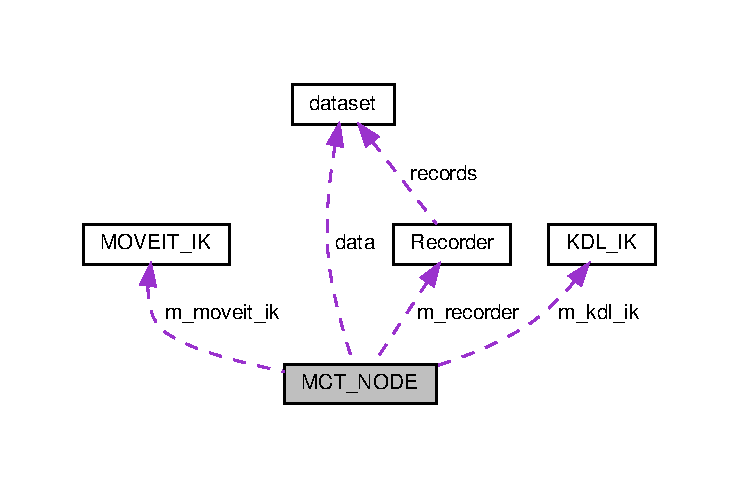
\includegraphics[width=350pt]{classMCT__NODE__coll__graph}
\end{center}
\end{figure}
\subsection*{Public Member Functions}
\begin{DoxyCompactItemize}
\item 
\mbox{\Hypertarget{classMCT__NODE_a212e93de8fe4595fd9e4593331f25984}\label{classMCT__NODE_a212e93de8fe4595fd9e4593331f25984}} 
\hyperlink{classMCT__NODE_a212e93de8fe4595fd9e4593331f25984}{M\+C\+T\+\_\+\+N\+O\+DE} ()
\begin{DoxyCompactList}\small\item\em Construct a new mct node object. \end{DoxyCompactList}\item 
\mbox{\Hypertarget{classMCT__NODE_a4817d20c20a700b5c9024f86951532fd}\label{classMCT__NODE_a4817d20c20a700b5c9024f86951532fd}} 
\hyperlink{classMCT__NODE_a4817d20c20a700b5c9024f86951532fd}{$\sim$\+M\+C\+T\+\_\+\+N\+O\+DE} ()
\begin{DoxyCompactList}\small\item\em Destroy the mct node object. \end{DoxyCompactList}\item 
\hyperlink{classMCT__NODE_a48aa593847730d011812896a11aa86e7}{M\+C\+T\+\_\+\+N\+O\+DE} (string str, \hyperlink{classRecorder}{Recorder} $\ast$recorder, \hyperlink{classMOVEIT__IK}{M\+O\+V\+E\+I\+T\+\_\+\+IK} $\ast$moveit\+\_\+ik, \hyperlink{classKDL__IK}{K\+D\+L\+\_\+\+IK} $\ast$kdl\+\_\+ik=N\+U\+LL)
\begin{DoxyCompactList}\small\item\em Construct a new mct node object. \end{DoxyCompactList}\item 
\mbox{\Hypertarget{classMCT__NODE_a0862ea70bd023be109c0297c9f90e5f4}\label{classMCT__NODE_a0862ea70bd023be109c0297c9f90e5f4}} 
void \hyperlink{classMCT__NODE_a0862ea70bd023be109c0297c9f90e5f4}{init} ()
\begin{DoxyCompactList}\small\item\em initialisation of node \end{DoxyCompactList}\item 
double \hyperlink{classMCT__NODE_a5adb70e08e5dac48147764d6922f6546}{update} ()
\begin{DoxyCompactList}\small\item\em update node score \end{DoxyCompactList}\item 
void \hyperlink{classMCT__NODE_a04ad1b7ce156c2501819d32047e3e83a}{set\+\_\+node\+\_\+idx} (int g, int a=-\/1, int s=-\/1, int p=-\/1)
\begin{DoxyCompactList}\small\item\em Set the node idx object. \end{DoxyCompactList}\item 
\mbox{\Hypertarget{classMCT__NODE_a411f350ef5e4d9ce85b361b6f7dfd512}\label{classMCT__NODE_a411f350ef5e4d9ce85b361b6f7dfd512}} 
void \hyperlink{classMCT__NODE_a411f350ef5e4d9ce85b361b6f7dfd512}{write\+\_\+dataset} ()
\begin{DoxyCompactList}\small\item\em Function to export node data to logger. \end{DoxyCompactList}\end{DoxyCompactItemize}
\subsection*{Public Attributes}
\begin{DoxyCompactItemize}
\item 
\mbox{\Hypertarget{classMCT__NODE_aed103b475b9ac51892f89c87463b8757}\label{classMCT__NODE_aed103b475b9ac51892f89c87463b8757}} 
string {\bfseries label}
\item 
\mbox{\Hypertarget{classMCT__NODE_ad5ec5cb688cefdd41776daad0e05a1e2}\label{classMCT__NODE_ad5ec5cb688cefdd41776daad0e05a1e2}} 
vector$<$ Affine3d $>$ {\bfseries state}
\item 
\mbox{\Hypertarget{classMCT__NODE_ac29a76b4d3b54f40260a6d151153f32d}\label{classMCT__NODE_ac29a76b4d3b54f40260a6d151153f32d}} 
vector$<$ Affine3d $>$ {\bfseries state2}
\item 
\mbox{\Hypertarget{classMCT__NODE_a8081b0320ef5642b231a432a06520181}\label{classMCT__NODE_a8081b0320ef5642b231a432a06520181}} 
vector$<$ Affine3d $>$ {\bfseries state3}
\item 
\mbox{\Hypertarget{classMCT__NODE_ac550ba83323e4d415ff6b6c99608439f}\label{classMCT__NODE_ac550ba83323e4d415ff6b6c99608439f}} 
Affine3d {\bfseries T\+\_\+tg}
\item 
\mbox{\Hypertarget{classMCT__NODE_a143531d5ca4a83852a3ba519cd390eeb}\label{classMCT__NODE_a143531d5ca4a83852a3ba519cd390eeb}} 
Affine3d {\bfseries T\+\_\+tf}
\item 
\mbox{\Hypertarget{classMCT__NODE_a364f2844d094010f5a3397db4b8e8849}\label{classMCT__NODE_a364f2844d094010f5a3397db4b8e8849}} 
bool {\bfseries small\+\_\+seg}
\item 
\mbox{\Hypertarget{classMCT__NODE_ae26c68e4e22b627657a5704a4e6e434f}\label{classMCT__NODE_ae26c68e4e22b627657a5704a4e6e434f}} 
double {\bfseries score}
\item 
\mbox{\Hypertarget{classMCT__NODE_a32f880a1f3a84b2f890b70178a15ec3b}\label{classMCT__NODE_a32f880a1f3a84b2f890b70178a15ec3b}} 
int {\bfseries num\+\_\+visit}
\item 
\mbox{\Hypertarget{classMCT__NODE_ac0493080d5fb0ad63946e8762d397db5}\label{classMCT__NODE_ac0493080d5fb0ad63946e8762d397db5}} 
double {\bfseries node\+\_\+value}
\item 
\mbox{\Hypertarget{classMCT__NODE_a89fecc3481363e9bea16776eb88c8b40}\label{classMCT__NODE_a89fecc3481363e9bea16776eb88c8b40}} 
vector$<$ \hyperlink{classMCT__NODE}{M\+C\+T\+\_\+\+N\+O\+DE} $>$ {\bfseries childs}
\item 
\mbox{\Hypertarget{classMCT__NODE_a3befbdb55ceb274d38bb16dc339a7d6f}\label{classMCT__NODE_a3befbdb55ceb274d38bb16dc339a7d6f}} 
int {\bfseries num\+\_\+childs}
\item 
\mbox{\Hypertarget{classMCT__NODE_a059636c69a0f512af7a949dcf2b57a4f}\label{classMCT__NODE_a059636c69a0f512af7a949dcf2b57a4f}} 
string {\bfseries type}
\item 
\mbox{\Hypertarget{classMCT__NODE_a024f5b5a02e9a31a57064a55466c34b7}\label{classMCT__NODE_a024f5b5a02e9a31a57064a55466c34b7}} 
Vector3d {\bfseries arm\+\_\+len}
\item 
\mbox{\Hypertarget{classMCT__NODE_ae1c0a686ad954f7d60f4084ed73e5cc3}\label{classMCT__NODE_ae1c0a686ad954f7d60f4084ed73e5cc3}} 
bool {\bfseries collision\+\_\+obj}
\end{DoxyCompactItemize}
\subsection*{Private Member Functions}
\begin{DoxyCompactItemize}
\item 
void \hyperlink{classMCT__NODE_aa6e0f2afcf3db54d05e6f6e4a6a31c0f}{update\+\_\+score} (double val)
\begin{DoxyCompactList}\small\item\em update the score of the node \end{DoxyCompactList}\item 
double \hyperlink{classMCT__NODE_aae9490861298c2419fe9c86991868c39}{calculate\+\_\+value} ()
\begin{DoxyCompactList}\small\item\em calculate the score of the node check if IK solution is possible, then score depends of the errors, delta of movement and etc. \end{DoxyCompactList}\item 
bool \hyperlink{classMCT__NODE_af3aca71d80572feca02667b2963bcf74}{all\+\_\+visited} ()
\begin{DoxyCompactList}\small\item\em check if this branch is all visited \end{DoxyCompactList}\end{DoxyCompactItemize}
\subsection*{Private Attributes}
\begin{DoxyCompactItemize}
\item 
\mbox{\Hypertarget{classMCT__NODE_aef874e890b766463e4759fc4d35ae953}\label{classMCT__NODE_aef874e890b766463e4759fc4d35ae953}} 
\hyperlink{classRecorder}{Recorder} $\ast$ {\bfseries m\+\_\+recorder}
\item 
\mbox{\Hypertarget{classMCT__NODE_a70703cea38d3318542b7273880d2dd85}\label{classMCT__NODE_a70703cea38d3318542b7273880d2dd85}} 
\hyperlink{classMOVEIT__IK}{M\+O\+V\+E\+I\+T\+\_\+\+IK} $\ast$ {\bfseries m\+\_\+moveit\+\_\+ik}
\item 
\mbox{\Hypertarget{classMCT__NODE_aa4771b9891fc59ff0c760066e2744798}\label{classMCT__NODE_aa4771b9891fc59ff0c760066e2744798}} 
\hyperlink{classKDL__IK}{K\+D\+L\+\_\+\+IK} $\ast$ {\bfseries m\+\_\+kdl\+\_\+ik}
\item 
\mbox{\Hypertarget{classMCT__NODE_a6eb1d731da9167a081b3551059e01364}\label{classMCT__NODE_a6eb1d731da9167a081b3551059e01364}} 
int \hyperlink{classMCT__NODE_a6eb1d731da9167a081b3551059e01364}{idx\+\_\+G}
\begin{DoxyCompactList}\small\item\em grasp idx \end{DoxyCompactList}\item 
\mbox{\Hypertarget{classMCT__NODE_a8584463b85cbb2d37e776e6b6b614333}\label{classMCT__NODE_a8584463b85cbb2d37e776e6b6b614333}} 
int \hyperlink{classMCT__NODE_a8584463b85cbb2d37e776e6b6b614333}{idx\+\_\+A}
\begin{DoxyCompactList}\small\item\em Attack angle of tool to object. \end{DoxyCompactList}\item 
\mbox{\Hypertarget{classMCT__NODE_a09749a6c804a3abe443868bb952177e0}\label{classMCT__NODE_a09749a6c804a3abe443868bb952177e0}} 
int \hyperlink{classMCT__NODE_a09749a6c804a3abe443868bb952177e0}{idx\+\_\+S}
\begin{DoxyCompactList}\small\item\em Segment index (is the segment wide or small?) \end{DoxyCompactList}\item 
\mbox{\Hypertarget{classMCT__NODE_a6796b0d15fdacaa0069ee9248dcb34db}\label{classMCT__NODE_a6796b0d15fdacaa0069ee9248dcb34db}} 
int \hyperlink{classMCT__NODE_a6796b0d15fdacaa0069ee9248dcb34db}{idx\+\_\+P}
\begin{DoxyCompactList}\small\item\em position index (which point of the tool does this node targets?) \end{DoxyCompactList}\item 
\mbox{\Hypertarget{classMCT__NODE_a82a084c7ba13283b6162bdecbb892878}\label{classMCT__NODE_a82a084c7ba13283b6162bdecbb892878}} 
\hyperlink{structdataset}{dataset} {\bfseries data}
\end{DoxyCompactItemize}


\subsection{Detailed Description}
class object for monte carlo tree search This is class for single node in the tree 

\subsection{Constructor \& Destructor Documentation}
\mbox{\Hypertarget{classMCT__NODE_a48aa593847730d011812896a11aa86e7}\label{classMCT__NODE_a48aa593847730d011812896a11aa86e7}} 
\index{M\+C\+T\+\_\+\+N\+O\+DE@{M\+C\+T\+\_\+\+N\+O\+DE}!M\+C\+T\+\_\+\+N\+O\+DE@{M\+C\+T\+\_\+\+N\+O\+DE}}
\index{M\+C\+T\+\_\+\+N\+O\+DE@{M\+C\+T\+\_\+\+N\+O\+DE}!M\+C\+T\+\_\+\+N\+O\+DE@{M\+C\+T\+\_\+\+N\+O\+DE}}
\subsubsection{\texorpdfstring{M\+C\+T\+\_\+\+N\+O\+D\+E()}{MCT\_NODE()}}
{\footnotesize\ttfamily M\+C\+T\+\_\+\+N\+O\+D\+E\+::\+M\+C\+T\+\_\+\+N\+O\+DE (\begin{DoxyParamCaption}\item[{string}]{str,  }\item[{\hyperlink{classRecorder}{Recorder} $\ast$}]{recorder,  }\item[{\hyperlink{classMOVEIT__IK}{M\+O\+V\+E\+I\+T\+\_\+\+IK} $\ast$}]{moveit\+\_\+ik,  }\item[{\hyperlink{classKDL__IK}{K\+D\+L\+\_\+\+IK} $\ast$}]{kdl\+\_\+ik = {\ttfamily NULL} }\end{DoxyParamCaption})\hspace{0.3cm}{\ttfamily [inline]}}



Construct a new mct node object. 


\begin{DoxyParams}{Parameters}
{\em str} & name \\
\hline
{\em recorder} & pointer to logging class \\
\hline
{\em moveit\+\_\+ik} & pointer to moveit IK solver class \\
\hline
{\em kdl\+\_\+ik} & pointer to kdl IK solver class \\
\hline
\end{DoxyParams}


\subsection{Member Function Documentation}
\mbox{\Hypertarget{classMCT__NODE_af3aca71d80572feca02667b2963bcf74}\label{classMCT__NODE_af3aca71d80572feca02667b2963bcf74}} 
\index{M\+C\+T\+\_\+\+N\+O\+DE@{M\+C\+T\+\_\+\+N\+O\+DE}!all\+\_\+visited@{all\+\_\+visited}}
\index{all\+\_\+visited@{all\+\_\+visited}!M\+C\+T\+\_\+\+N\+O\+DE@{M\+C\+T\+\_\+\+N\+O\+DE}}
\subsubsection{\texorpdfstring{all\+\_\+visited()}{all\_visited()}}
{\footnotesize\ttfamily bool M\+C\+T\+\_\+\+N\+O\+D\+E\+::all\+\_\+visited (\begin{DoxyParamCaption}{ }\end{DoxyParamCaption})\hspace{0.3cm}{\ttfamily [private]}}



check if this branch is all visited 

\begin{DoxyReturn}{Returns}
true visited 

false not finished 
\end{DoxyReturn}
\mbox{\Hypertarget{classMCT__NODE_aae9490861298c2419fe9c86991868c39}\label{classMCT__NODE_aae9490861298c2419fe9c86991868c39}} 
\index{M\+C\+T\+\_\+\+N\+O\+DE@{M\+C\+T\+\_\+\+N\+O\+DE}!calculate\+\_\+value@{calculate\+\_\+value}}
\index{calculate\+\_\+value@{calculate\+\_\+value}!M\+C\+T\+\_\+\+N\+O\+DE@{M\+C\+T\+\_\+\+N\+O\+DE}}
\subsubsection{\texorpdfstring{calculate\+\_\+value()}{calculate\_value()}}
{\footnotesize\ttfamily double M\+C\+T\+\_\+\+N\+O\+D\+E\+::calculate\+\_\+value (\begin{DoxyParamCaption}{ }\end{DoxyParamCaption})\hspace{0.3cm}{\ttfamily [private]}}



calculate the score of the node check if IK solution is possible, then score depends of the errors, delta of movement and etc. 

\begin{DoxyReturn}{Returns}
double score value 
\end{DoxyReturn}
\mbox{\Hypertarget{classMCT__NODE_a04ad1b7ce156c2501819d32047e3e83a}\label{classMCT__NODE_a04ad1b7ce156c2501819d32047e3e83a}} 
\index{M\+C\+T\+\_\+\+N\+O\+DE@{M\+C\+T\+\_\+\+N\+O\+DE}!set\+\_\+node\+\_\+idx@{set\+\_\+node\+\_\+idx}}
\index{set\+\_\+node\+\_\+idx@{set\+\_\+node\+\_\+idx}!M\+C\+T\+\_\+\+N\+O\+DE@{M\+C\+T\+\_\+\+N\+O\+DE}}
\subsubsection{\texorpdfstring{set\+\_\+node\+\_\+idx()}{set\_node\_idx()}}
{\footnotesize\ttfamily void M\+C\+T\+\_\+\+N\+O\+D\+E\+::set\+\_\+node\+\_\+idx (\begin{DoxyParamCaption}\item[{int}]{g,  }\item[{int}]{a = {\ttfamily -\/1},  }\item[{int}]{s = {\ttfamily -\/1},  }\item[{int}]{p = {\ttfamily -\/1} }\end{DoxyParamCaption})\hspace{0.3cm}{\ttfamily [inline]}}



Set the node idx object. 


\begin{DoxyParams}{Parameters}
{\em g} & \\
\hline
{\em a} & \\
\hline
{\em s} & \\
\hline
{\em p} & \\
\hline
\end{DoxyParams}
\mbox{\Hypertarget{classMCT__NODE_a5adb70e08e5dac48147764d6922f6546}\label{classMCT__NODE_a5adb70e08e5dac48147764d6922f6546}} 
\index{M\+C\+T\+\_\+\+N\+O\+DE@{M\+C\+T\+\_\+\+N\+O\+DE}!update@{update}}
\index{update@{update}!M\+C\+T\+\_\+\+N\+O\+DE@{M\+C\+T\+\_\+\+N\+O\+DE}}
\subsubsection{\texorpdfstring{update()}{update()}}
{\footnotesize\ttfamily double M\+C\+T\+\_\+\+N\+O\+D\+E\+::update (\begin{DoxyParamCaption}{ }\end{DoxyParamCaption})}



update node score 

\begin{DoxyReturn}{Returns}
double score 
\end{DoxyReturn}
\mbox{\Hypertarget{classMCT__NODE_aa6e0f2afcf3db54d05e6f6e4a6a31c0f}\label{classMCT__NODE_aa6e0f2afcf3db54d05e6f6e4a6a31c0f}} 
\index{M\+C\+T\+\_\+\+N\+O\+DE@{M\+C\+T\+\_\+\+N\+O\+DE}!update\+\_\+score@{update\+\_\+score}}
\index{update\+\_\+score@{update\+\_\+score}!M\+C\+T\+\_\+\+N\+O\+DE@{M\+C\+T\+\_\+\+N\+O\+DE}}
\subsubsection{\texorpdfstring{update\+\_\+score()}{update\_score()}}
{\footnotesize\ttfamily void M\+C\+T\+\_\+\+N\+O\+D\+E\+::update\+\_\+score (\begin{DoxyParamCaption}\item[{double}]{val }\end{DoxyParamCaption})\hspace{0.3cm}{\ttfamily [private]}}



update the score of the node 


\begin{DoxyParams}{Parameters}
{\em val} & \\
\hline
\end{DoxyParams}


The documentation for this class was generated from the following files\+:\begin{DoxyCompactItemize}
\item 
/home/samuel/\+Desktop/toolcog\+\_\+ws/montecarlo/include/tool\+\_\+expt/\hyperlink{node_8h}{node.\+h}\item 
/home/samuel/\+Desktop/toolcog\+\_\+ws/montecarlo/src/node.\+cpp\end{DoxyCompactItemize}

\hypertarget{classMCT__NODE2}{}\section{M\+C\+T\+\_\+\+N\+O\+D\+E2 Class Reference}
\label{classMCT__NODE2}\index{M\+C\+T\+\_\+\+N\+O\+D\+E2@{M\+C\+T\+\_\+\+N\+O\+D\+E2}}


class object for monte carlo tree search This is class for single node in the tree version 2.\+0, setup node to perform as a recursive function  




{\ttfamily \#include $<$node2.\+h$>$}



Collaboration diagram for M\+C\+T\+\_\+\+N\+O\+D\+E2\+:
\nopagebreak
\begin{figure}[H]
\begin{center}
\leavevmode
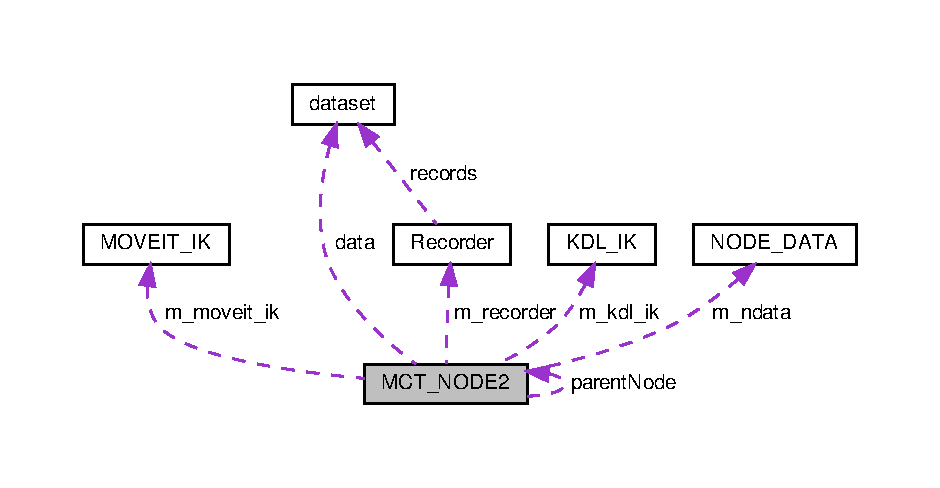
\includegraphics[width=350pt]{classMCT__NODE2__coll__graph}
\end{center}
\end{figure}
\subsection*{Public Member Functions}
\begin{DoxyCompactItemize}
\item 
\mbox{\Hypertarget{classMCT__NODE2_a79a6d3015439b33c46ba184dc314f5e4}\label{classMCT__NODE2_a79a6d3015439b33c46ba184dc314f5e4}} 
\hyperlink{classMCT__NODE2_a79a6d3015439b33c46ba184dc314f5e4}{M\+C\+T\+\_\+\+N\+O\+D\+E2} ()
\begin{DoxyCompactList}\small\item\em Construct a new mct node2 object. \end{DoxyCompactList}\item 
\mbox{\Hypertarget{classMCT__NODE2_a180c6f50288efb2b93a44872b14e4d5e}\label{classMCT__NODE2_a180c6f50288efb2b93a44872b14e4d5e}} 
\hyperlink{classMCT__NODE2_a180c6f50288efb2b93a44872b14e4d5e}{$\sim$\+M\+C\+T\+\_\+\+N\+O\+D\+E2} ()
\begin{DoxyCompactList}\small\item\em Destroy the mct node2 object. \end{DoxyCompactList}\item 
\hyperlink{classMCT__NODE2_a729c4d4e44b9de40835e51abb915008f}{M\+C\+T\+\_\+\+N\+O\+D\+E2} (string str, \hyperlink{structNODE__DATA}{N\+O\+D\+E\+\_\+\+D\+A\+TA} ndata, \hyperlink{classRecorder}{Recorder} $\ast$recorder, \hyperlink{classMOVEIT__IK}{M\+O\+V\+E\+I\+T\+\_\+\+IK} $\ast$moveit\+\_\+ik, \hyperlink{classKDL__IK}{K\+D\+L\+\_\+\+IK} $\ast$kdl\+\_\+ik=N\+U\+LL)
\begin{DoxyCompactList}\small\item\em Construct a new mct node2 object. \end{DoxyCompactList}\item 
\hyperlink{classMCT__NODE2_a8a3bb30fd398361d821d04a10f311a68}{M\+C\+T\+\_\+\+N\+O\+D\+E2} (\hyperlink{classMCT__NODE2}{M\+C\+T\+\_\+\+N\+O\+D\+E2} $\ast$parent, string str, \hyperlink{structNODE__DATA}{N\+O\+D\+E\+\_\+\+D\+A\+TA} ndata, \hyperlink{classRecorder}{Recorder} $\ast$recorder, \hyperlink{classMOVEIT__IK}{M\+O\+V\+E\+I\+T\+\_\+\+IK} $\ast$moveit\+\_\+ik, \hyperlink{classKDL__IK}{K\+D\+L\+\_\+\+IK} $\ast$kdl\+\_\+ik=N\+U\+LL)
\begin{DoxyCompactList}\small\item\em Construct a new mct node2 object. \end{DoxyCompactList}\item 
void \hyperlink{classMCT__NODE2_ab7b3824130219c1afdfd8d8358e52d76}{create\+\_\+child} (string str, \hyperlink{structNODE__DATA}{N\+O\+D\+E\+\_\+\+D\+A\+TA} ndata)
\begin{DoxyCompactList}\small\item\em Create a child object. \end{DoxyCompactList}\item 
\mbox{\Hypertarget{classMCT__NODE2_a50143d6d92d93c4ede150b6b10c7dcab}\label{classMCT__NODE2_a50143d6d92d93c4ede150b6b10c7dcab}} 
void \hyperlink{classMCT__NODE2_a50143d6d92d93c4ede150b6b10c7dcab}{init} ()
\begin{DoxyCompactList}\small\item\em initialisation of node \end{DoxyCompactList}\item 
double \hyperlink{classMCT__NODE2_a02b11b2ef3bc916dc8bb7fec7f475ca7}{update} ()
\begin{DoxyCompactList}\small\item\em update node score \end{DoxyCompactList}\item 
\mbox{\Hypertarget{classMCT__NODE2_a519001f81d9ed6e03cbd026d8c94bafa}\label{classMCT__NODE2_a519001f81d9ed6e03cbd026d8c94bafa}} 
void \hyperlink{classMCT__NODE2_a519001f81d9ed6e03cbd026d8c94bafa}{write\+\_\+dataset} ()
\begin{DoxyCompactList}\small\item\em Function to export node data to logger. \end{DoxyCompactList}\end{DoxyCompactItemize}
\subsection*{Public Attributes}
\begin{DoxyCompactItemize}
\item 
\mbox{\Hypertarget{classMCT__NODE2_a9a39405216826460e11b0865556ee0db}\label{classMCT__NODE2_a9a39405216826460e11b0865556ee0db}} 
\hyperlink{classMCT__NODE2}{M\+C\+T\+\_\+\+N\+O\+D\+E2} $\ast$ {\bfseries parent\+Node}
\item 
\mbox{\Hypertarget{classMCT__NODE2_aa60c90f3cbbcd3e355d7de9675048e7a}\label{classMCT__NODE2_aa60c90f3cbbcd3e355d7de9675048e7a}} 
vector$<$ \hyperlink{classMCT__NODE2}{M\+C\+T\+\_\+\+N\+O\+D\+E2} $\ast$$>$ {\bfseries childs}
\item 
\mbox{\Hypertarget{classMCT__NODE2_a0e77e9354445bfc3609d50687179c76a}\label{classMCT__NODE2_a0e77e9354445bfc3609d50687179c76a}} 
string {\bfseries label}
\item 
\mbox{\Hypertarget{classMCT__NODE2_a0e7e94393ff13d35c204f0008f194b21}\label{classMCT__NODE2_a0e7e94393ff13d35c204f0008f194b21}} 
double {\bfseries score}
\item 
\mbox{\Hypertarget{classMCT__NODE2_aea3632ed0982534dee1f4a60d56c3f21}\label{classMCT__NODE2_aea3632ed0982534dee1f4a60d56c3f21}} 
double {\bfseries node\+\_\+value}
\item 
\mbox{\Hypertarget{classMCT__NODE2_a613a6cf94f700df93f2d17d75cef5551}\label{classMCT__NODE2_a613a6cf94f700df93f2d17d75cef5551}} 
int {\bfseries num\+\_\+visit}
\item 
\mbox{\Hypertarget{classMCT__NODE2_a287d39d9355208167d8af1859844d0bf}\label{classMCT__NODE2_a287d39d9355208167d8af1859844d0bf}} 
int {\bfseries num\+\_\+childs}
\item 
\mbox{\Hypertarget{classMCT__NODE2_aa1e45aad90bb598289fb34c4da3971a0}\label{classMCT__NODE2_aa1e45aad90bb598289fb34c4da3971a0}} 
string {\bfseries type}
\item 
\mbox{\Hypertarget{classMCT__NODE2_af82fcb1cce3a71b11d5d4f7309fa4ea9}\label{classMCT__NODE2_af82fcb1cce3a71b11d5d4f7309fa4ea9}} 
Vector3d {\bfseries arm\+\_\+len}
\item 
\mbox{\Hypertarget{classMCT__NODE2_a30bd8b8058d5480cf5adfe53e621e0f5}\label{classMCT__NODE2_a30bd8b8058d5480cf5adfe53e621e0f5}} 
\hyperlink{structNODE__DATA}{N\+O\+D\+E\+\_\+\+D\+A\+TA} {\bfseries m\+\_\+ndata}
\item 
\mbox{\Hypertarget{classMCT__NODE2_aaeabafd0d4bd2e7ed2304cfad542937e}\label{classMCT__NODE2_aaeabafd0d4bd2e7ed2304cfad542937e}} 
double {\bfseries best\+\_\+score}
\item 
\mbox{\Hypertarget{classMCT__NODE2_a4169d8ff91cf7cd1e83e3899bcead531}\label{classMCT__NODE2_a4169d8ff91cf7cd1e83e3899bcead531}} 
vector$<$ int $>$ {\bfseries best\+\_\+idx}
\item 
\mbox{\Hypertarget{classMCT__NODE2_a786433c1043c2f6659e69893e66d4bc7}\label{classMCT__NODE2_a786433c1043c2f6659e69893e66d4bc7}} 
vector$<$ Affine3d $>$ {\bfseries best\+\_\+state}
\end{DoxyCompactItemize}
\subsection*{Private Member Functions}
\begin{DoxyCompactItemize}
\item 
void \hyperlink{classMCT__NODE2_a7e14b83901a94e54e3ef87aa012078de}{update\+\_\+score} (double val)
\begin{DoxyCompactList}\small\item\em update the score of the node \end{DoxyCompactList}\item 
double \hyperlink{classMCT__NODE2_a54908b7091bfc9ef49c06b2310d94408}{calculate\+\_\+value} ()
\begin{DoxyCompactList}\small\item\em calculate the score of the node check if IK solution is possible, then score depends of the errors, delta of movement, the size of the segment, the grasping position, the attack angle of the tool to object and etc. \end{DoxyCompactList}\item 
bool \hyperlink{classMCT__NODE2_a86c2a067b3865746d0a1b39142c0c536}{all\+\_\+visited} ()
\begin{DoxyCompactList}\small\item\em check if this branch \& child are all visited \end{DoxyCompactList}\end{DoxyCompactItemize}
\subsection*{Private Attributes}
\begin{DoxyCompactItemize}
\item 
\mbox{\Hypertarget{classMCT__NODE2_a8938cf11d3628ac8275515d2d8e56f3e}\label{classMCT__NODE2_a8938cf11d3628ac8275515d2d8e56f3e}} 
\hyperlink{classRecorder}{Recorder} $\ast$ {\bfseries m\+\_\+recorder}
\item 
\mbox{\Hypertarget{classMCT__NODE2_acbda5193b6d56d41dadce675e6ca4874}\label{classMCT__NODE2_acbda5193b6d56d41dadce675e6ca4874}} 
\hyperlink{classMOVEIT__IK}{M\+O\+V\+E\+I\+T\+\_\+\+IK} $\ast$ {\bfseries m\+\_\+moveit\+\_\+ik}
\item 
\mbox{\Hypertarget{classMCT__NODE2_aeb643d23a87bf5a2ef8a0058f4188abc}\label{classMCT__NODE2_aeb643d23a87bf5a2ef8a0058f4188abc}} 
\hyperlink{classKDL__IK}{K\+D\+L\+\_\+\+IK} $\ast$ {\bfseries m\+\_\+kdl\+\_\+ik}
\item 
\mbox{\Hypertarget{classMCT__NODE2_a01fce094b0953fbd4269a22d4d77a9c4}\label{classMCT__NODE2_a01fce094b0953fbd4269a22d4d77a9c4}} 
\hyperlink{structdataset}{dataset} {\bfseries data}
\end{DoxyCompactItemize}


\subsection{Detailed Description}
class object for monte carlo tree search This is class for single node in the tree version 2.\+0, setup node to perform as a recursive function 

\subsection{Constructor \& Destructor Documentation}
\mbox{\Hypertarget{classMCT__NODE2_a729c4d4e44b9de40835e51abb915008f}\label{classMCT__NODE2_a729c4d4e44b9de40835e51abb915008f}} 
\index{M\+C\+T\+\_\+\+N\+O\+D\+E2@{M\+C\+T\+\_\+\+N\+O\+D\+E2}!M\+C\+T\+\_\+\+N\+O\+D\+E2@{M\+C\+T\+\_\+\+N\+O\+D\+E2}}
\index{M\+C\+T\+\_\+\+N\+O\+D\+E2@{M\+C\+T\+\_\+\+N\+O\+D\+E2}!M\+C\+T\+\_\+\+N\+O\+D\+E2@{M\+C\+T\+\_\+\+N\+O\+D\+E2}}
\subsubsection{\texorpdfstring{M\+C\+T\+\_\+\+N\+O\+D\+E2()}{MCT\_NODE2()}\hspace{0.1cm}{\footnotesize\ttfamily [1/2]}}
{\footnotesize\ttfamily M\+C\+T\+\_\+\+N\+O\+D\+E2\+::\+M\+C\+T\+\_\+\+N\+O\+D\+E2 (\begin{DoxyParamCaption}\item[{string}]{str,  }\item[{\hyperlink{structNODE__DATA}{N\+O\+D\+E\+\_\+\+D\+A\+TA}}]{ndata,  }\item[{\hyperlink{classRecorder}{Recorder} $\ast$}]{recorder,  }\item[{\hyperlink{classMOVEIT__IK}{M\+O\+V\+E\+I\+T\+\_\+\+IK} $\ast$}]{moveit\+\_\+ik,  }\item[{\hyperlink{classKDL__IK}{K\+D\+L\+\_\+\+IK} $\ast$}]{kdl\+\_\+ik = {\ttfamily NULL} }\end{DoxyParamCaption})\hspace{0.3cm}{\ttfamily [inline]}}



Construct a new mct node2 object. 


\begin{DoxyParams}{Parameters}
{\em str} & name \\
\hline
{\em ndata} & node data \\
\hline
{\em recorder} & pointer to logging class obj \\
\hline
{\em moveit\+\_\+ik} & pointer to moveit IK solver class obj \\
\hline
{\em kdl\+\_\+ik} & pointer to kdl IK solver class obj \\
\hline
\end{DoxyParams}
\mbox{\Hypertarget{classMCT__NODE2_a8a3bb30fd398361d821d04a10f311a68}\label{classMCT__NODE2_a8a3bb30fd398361d821d04a10f311a68}} 
\index{M\+C\+T\+\_\+\+N\+O\+D\+E2@{M\+C\+T\+\_\+\+N\+O\+D\+E2}!M\+C\+T\+\_\+\+N\+O\+D\+E2@{M\+C\+T\+\_\+\+N\+O\+D\+E2}}
\index{M\+C\+T\+\_\+\+N\+O\+D\+E2@{M\+C\+T\+\_\+\+N\+O\+D\+E2}!M\+C\+T\+\_\+\+N\+O\+D\+E2@{M\+C\+T\+\_\+\+N\+O\+D\+E2}}
\subsubsection{\texorpdfstring{M\+C\+T\+\_\+\+N\+O\+D\+E2()}{MCT\_NODE2()}\hspace{0.1cm}{\footnotesize\ttfamily [2/2]}}
{\footnotesize\ttfamily M\+C\+T\+\_\+\+N\+O\+D\+E2\+::\+M\+C\+T\+\_\+\+N\+O\+D\+E2 (\begin{DoxyParamCaption}\item[{\hyperlink{classMCT__NODE2}{M\+C\+T\+\_\+\+N\+O\+D\+E2} $\ast$}]{parent,  }\item[{string}]{str,  }\item[{\hyperlink{structNODE__DATA}{N\+O\+D\+E\+\_\+\+D\+A\+TA}}]{ndata,  }\item[{\hyperlink{classRecorder}{Recorder} $\ast$}]{recorder,  }\item[{\hyperlink{classMOVEIT__IK}{M\+O\+V\+E\+I\+T\+\_\+\+IK} $\ast$}]{moveit\+\_\+ik,  }\item[{\hyperlink{classKDL__IK}{K\+D\+L\+\_\+\+IK} $\ast$}]{kdl\+\_\+ik = {\ttfamily NULL} }\end{DoxyParamCaption})\hspace{0.3cm}{\ttfamily [inline]}}



Construct a new mct node2 object. 


\begin{DoxyParams}{Parameters}
{\em parent} & pointer to parent node \\
\hline
{\em str} & name \\
\hline
{\em ndata} & node data \\
\hline
{\em recorder} & pointer to logging class obj \\
\hline
{\em moveit\+\_\+ik} & pointer to moveit IK solver class obj \\
\hline
{\em kdl\+\_\+ik} & pointer to kdl IK solver class obj \\
\hline
\end{DoxyParams}


\subsection{Member Function Documentation}
\mbox{\Hypertarget{classMCT__NODE2_a86c2a067b3865746d0a1b39142c0c536}\label{classMCT__NODE2_a86c2a067b3865746d0a1b39142c0c536}} 
\index{M\+C\+T\+\_\+\+N\+O\+D\+E2@{M\+C\+T\+\_\+\+N\+O\+D\+E2}!all\+\_\+visited@{all\+\_\+visited}}
\index{all\+\_\+visited@{all\+\_\+visited}!M\+C\+T\+\_\+\+N\+O\+D\+E2@{M\+C\+T\+\_\+\+N\+O\+D\+E2}}
\subsubsection{\texorpdfstring{all\+\_\+visited()}{all\_visited()}}
{\footnotesize\ttfamily bool M\+C\+T\+\_\+\+N\+O\+D\+E2\+::all\+\_\+visited (\begin{DoxyParamCaption}{ }\end{DoxyParamCaption})\hspace{0.3cm}{\ttfamily [private]}}



check if this branch \& child are all visited 

\begin{DoxyReturn}{Returns}
true visited 

false not finished 
\end{DoxyReturn}
\mbox{\Hypertarget{classMCT__NODE2_a54908b7091bfc9ef49c06b2310d94408}\label{classMCT__NODE2_a54908b7091bfc9ef49c06b2310d94408}} 
\index{M\+C\+T\+\_\+\+N\+O\+D\+E2@{M\+C\+T\+\_\+\+N\+O\+D\+E2}!calculate\+\_\+value@{calculate\+\_\+value}}
\index{calculate\+\_\+value@{calculate\+\_\+value}!M\+C\+T\+\_\+\+N\+O\+D\+E2@{M\+C\+T\+\_\+\+N\+O\+D\+E2}}
\subsubsection{\texorpdfstring{calculate\+\_\+value()}{calculate\_value()}}
{\footnotesize\ttfamily double M\+C\+T\+\_\+\+N\+O\+D\+E2\+::calculate\+\_\+value (\begin{DoxyParamCaption}{ }\end{DoxyParamCaption})\hspace{0.3cm}{\ttfamily [private]}}



calculate the score of the node check if IK solution is possible, then score depends of the errors, delta of movement, the size of the segment, the grasping position, the attack angle of the tool to object and etc. 

\begin{DoxyReturn}{Returns}
double score value 
\end{DoxyReturn}
\mbox{\Hypertarget{classMCT__NODE2_ab7b3824130219c1afdfd8d8358e52d76}\label{classMCT__NODE2_ab7b3824130219c1afdfd8d8358e52d76}} 
\index{M\+C\+T\+\_\+\+N\+O\+D\+E2@{M\+C\+T\+\_\+\+N\+O\+D\+E2}!create\+\_\+child@{create\+\_\+child}}
\index{create\+\_\+child@{create\+\_\+child}!M\+C\+T\+\_\+\+N\+O\+D\+E2@{M\+C\+T\+\_\+\+N\+O\+D\+E2}}
\subsubsection{\texorpdfstring{create\+\_\+child()}{create\_child()}}
{\footnotesize\ttfamily void M\+C\+T\+\_\+\+N\+O\+D\+E2\+::create\+\_\+child (\begin{DoxyParamCaption}\item[{string}]{str,  }\item[{\hyperlink{structNODE__DATA}{N\+O\+D\+E\+\_\+\+D\+A\+TA}}]{ndata }\end{DoxyParamCaption})}



Create a child object. 


\begin{DoxyParams}{Parameters}
{\em str} & name \\
\hline
{\em ndata} & node data \\
\hline
\end{DoxyParams}
\mbox{\Hypertarget{classMCT__NODE2_a02b11b2ef3bc916dc8bb7fec7f475ca7}\label{classMCT__NODE2_a02b11b2ef3bc916dc8bb7fec7f475ca7}} 
\index{M\+C\+T\+\_\+\+N\+O\+D\+E2@{M\+C\+T\+\_\+\+N\+O\+D\+E2}!update@{update}}
\index{update@{update}!M\+C\+T\+\_\+\+N\+O\+D\+E2@{M\+C\+T\+\_\+\+N\+O\+D\+E2}}
\subsubsection{\texorpdfstring{update()}{update()}}
{\footnotesize\ttfamily double M\+C\+T\+\_\+\+N\+O\+D\+E2\+::update (\begin{DoxyParamCaption}{ }\end{DoxyParamCaption})}



update node score 

\begin{DoxyReturn}{Returns}
double score 
\end{DoxyReturn}
\mbox{\Hypertarget{classMCT__NODE2_a7e14b83901a94e54e3ef87aa012078de}\label{classMCT__NODE2_a7e14b83901a94e54e3ef87aa012078de}} 
\index{M\+C\+T\+\_\+\+N\+O\+D\+E2@{M\+C\+T\+\_\+\+N\+O\+D\+E2}!update\+\_\+score@{update\+\_\+score}}
\index{update\+\_\+score@{update\+\_\+score}!M\+C\+T\+\_\+\+N\+O\+D\+E2@{M\+C\+T\+\_\+\+N\+O\+D\+E2}}
\subsubsection{\texorpdfstring{update\+\_\+score()}{update\_score()}}
{\footnotesize\ttfamily void M\+C\+T\+\_\+\+N\+O\+D\+E2\+::update\+\_\+score (\begin{DoxyParamCaption}\item[{double}]{val }\end{DoxyParamCaption})\hspace{0.3cm}{\ttfamily [private]}}



update the score of the node 


\begin{DoxyParams}{Parameters}
{\em val} & \\
\hline
\end{DoxyParams}


The documentation for this class was generated from the following files\+:\begin{DoxyCompactItemize}
\item 
/home/samuel/\+Desktop/toolcog\+\_\+ws/montecarlo/include/tool\+\_\+expt/\hyperlink{node2_8h}{node2.\+h}\item 
/home/samuel/\+Desktop/toolcog\+\_\+ws/montecarlo/src/node2.\+cpp\end{DoxyCompactItemize}

\hypertarget{classMCT__Search}{}\section{M\+C\+T\+\_\+\+Search Class Reference}
\label{classMCT__Search}\index{M\+C\+T\+\_\+\+Search@{M\+C\+T\+\_\+\+Search}}


Class object to perform monte carlo tree search algorithm.  




{\ttfamily \#include $<$search.\+h$>$}



Collaboration diagram for M\+C\+T\+\_\+\+Search\+:
\nopagebreak
\begin{figure}[H]
\begin{center}
\leavevmode
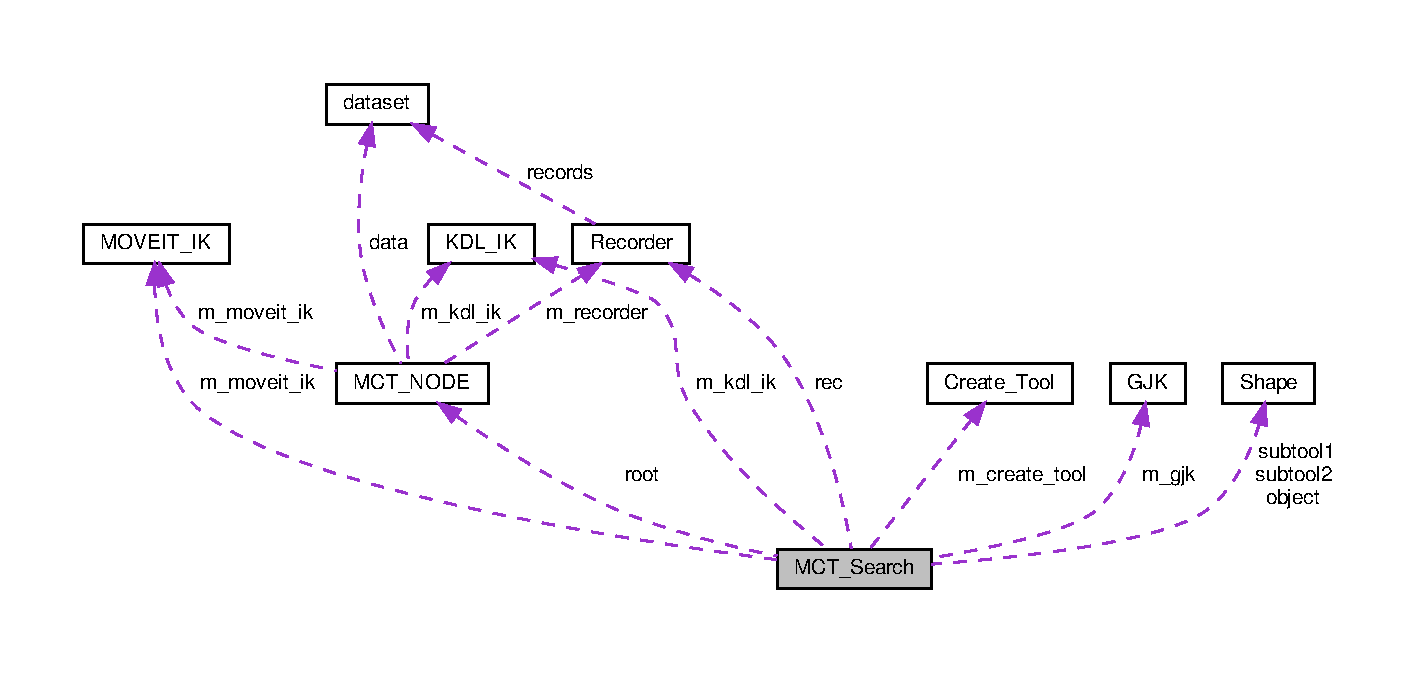
\includegraphics[width=350pt]{classMCT__Search__coll__graph}
\end{center}
\end{figure}
\subsection*{Public Member Functions}
\begin{DoxyCompactItemize}
\item 
\mbox{\Hypertarget{classMCT__Search_ad8edd41370fd1a382dc722e03f362d7c}\label{classMCT__Search_ad8edd41370fd1a382dc722e03f362d7c}} 
\hyperlink{classMCT__Search_ad8edd41370fd1a382dc722e03f362d7c}{M\+C\+T\+\_\+\+Search} ()
\begin{DoxyCompactList}\small\item\em Construct a new mct search object. \end{DoxyCompactList}\item 
\mbox{\Hypertarget{classMCT__Search_a8eae1473dc5cc84c857f0cf26bfda769}\label{classMCT__Search_a8eae1473dc5cc84c857f0cf26bfda769}} 
\hyperlink{classMCT__Search_a8eae1473dc5cc84c857f0cf26bfda769}{$\sim$\+M\+C\+T\+\_\+\+Search} ()
\begin{DoxyCompactList}\small\item\em Destroy the mct search object. \end{DoxyCompactList}\item 
void \hyperlink{classMCT__Search_a616c197a5427596143c0512a40373e8d}{init} (\hyperlink{classCreate__Tool}{Create\+\_\+\+Tool} $\ast$create\+\_\+tool, \hyperlink{classMOVEIT__IK}{M\+O\+V\+E\+I\+T\+\_\+\+IK} $\ast$moveit\+\_\+ik, \hyperlink{classKDL__IK}{K\+D\+L\+\_\+\+IK} $\ast$kdl\+\_\+ik=N\+U\+LL)
\begin{DoxyCompactList}\small\item\em initialise class object \end{DoxyCompactList}\item 
void \hyperlink{classMCT__Search_a42deaa445456fd8d1f286ab7c62f3714}{init\+\_\+params} (int num\+\_\+grasp, int num\+\_\+atk\+\_\+angle, int plays=500)
\begin{DoxyCompactList}\small\item\em initialise other parameters for M\+C\+TS consideration \end{DoxyCompactList}\item 
\mbox{\Hypertarget{classMCT__Search_a908f154a160cadebf1c873425ffb0dee}\label{classMCT__Search_a908f154a160cadebf1c873425ffb0dee}} 
void \hyperlink{classMCT__Search_a908f154a160cadebf1c873425ffb0dee}{search} ()
\begin{DoxyCompactList}\small\item\em start the M\+C\+TS search \end{DoxyCompactList}\item 
vector$<$ Affine3d $>$ \hyperlink{classMCT__Search_ab28fe87c4254e464ab8cfce14ffc665e}{get\+Result} ()
\begin{DoxyCompactList}\small\item\em Get the Resulting best Path to follow to pull/push object. \end{DoxyCompactList}\item 
Affine3d \hyperlink{classMCT__Search_a924b943dc6a98886ada00eb596d04e1c}{get\+Grab} ()
\begin{DoxyCompactList}\small\item\em Get the Resulting best Grab pose. \end{DoxyCompactList}\item 
double \hyperlink{classMCT__Search_ac21fe2ffab807bfcc9c8da9863791433}{get\+Atk\+Angle} ()
\begin{DoxyCompactList}\small\item\em Get the Resulting best attach angle of the tool to object. \end{DoxyCompactList}\item 
double \hyperlink{classMCT__Search_aa7029de4d31d20f106ce215affca20e0}{get\+Score} ()
\begin{DoxyCompactList}\small\item\em Get the Score of the best solution. \end{DoxyCompactList}\end{DoxyCompactItemize}
\subsection*{Public Attributes}
\begin{DoxyCompactItemize}
\item 
\mbox{\Hypertarget{classMCT__Search_a054354b0c101f6c8ab122781f5bf965f}\label{classMCT__Search_a054354b0c101f6c8ab122781f5bf965f}} 
int {\bfseries N\+\_\+via\+\_\+pts}
\item 
\mbox{\Hypertarget{classMCT__Search_af841697d9d2cfb2fe9f82b1f6254c7b9}\label{classMCT__Search_af841697d9d2cfb2fe9f82b1f6254c7b9}} 
int {\bfseries N\+\_\+intrapath\+\_\+pts}
\item 
\mbox{\Hypertarget{classMCT__Search_a86a1f14b3fe6dd32ac77fa328e1b0713}\label{classMCT__Search_a86a1f14b3fe6dd32ac77fa328e1b0713}} 
int {\bfseries N\+\_\+path\+\_\+pts}
\item 
\mbox{\Hypertarget{classMCT__Search_adda65004d78d9716fe508db26eb4580d}\label{classMCT__Search_adda65004d78d9716fe508db26eb4580d}} 
int {\bfseries max\+\_\+iter}
\item 
\mbox{\Hypertarget{classMCT__Search_a1b51bdf4a8a7a606bd4ee7a40bc9bc37}\label{classMCT__Search_a1b51bdf4a8a7a606bd4ee7a40bc9bc37}} 
vector$<$ Affine3d $>$ {\bfseries T\+\_\+world\+\_\+obj}
\item 
\mbox{\Hypertarget{classMCT__Search_ac67fcdc0e82da528f730f235a29388d4}\label{classMCT__Search_ac67fcdc0e82da528f730f235a29388d4}} 
vector$<$ Affine3d $>$ {\bfseries T\+\_\+obj\+\_\+func}
\item 
\mbox{\Hypertarget{classMCT__Search_a0cde1b8c3137cba8d20c01d3495ce934}\label{classMCT__Search_a0cde1b8c3137cba8d20c01d3495ce934}} 
Affine3d {\bfseries T\+\_\+obj\+\_\+task}
\item 
\mbox{\Hypertarget{classMCT__Search_ac01ec3e30dedbb73cb161d16595858c8}\label{classMCT__Search_ac01ec3e30dedbb73cb161d16595858c8}} 
\hyperlink{structShape}{Shape} {\bfseries subtool1}
\item 
\mbox{\Hypertarget{classMCT__Search_a556d98ae62d0a72d1b7297ddbdc909ca}\label{classMCT__Search_a556d98ae62d0a72d1b7297ddbdc909ca}} 
\hyperlink{structShape}{Shape} {\bfseries subtool2}
\item 
\mbox{\Hypertarget{classMCT__Search_acc3c7f8c1fd8268af823ac3e3d775820}\label{classMCT__Search_acc3c7f8c1fd8268af823ac3e3d775820}} 
\hyperlink{structShape}{Shape} {\bfseries object}
\item 
\mbox{\Hypertarget{classMCT__Search_a4064b83c8a8af24917ac7c416414c954}\label{classMCT__Search_a4064b83c8a8af24917ac7c416414c954}} 
vector$<$ Affine3d $>$ {\bfseries grasp\+\_\+loci}
\item 
\mbox{\Hypertarget{classMCT__Search_a915954e9c2eec4575ef471d6b9e63131}\label{classMCT__Search_a915954e9c2eec4575ef471d6b9e63131}} 
bool {\bfseries percept\+Flag}
\item 
\mbox{\Hypertarget{classMCT__Search_a52862592a8434d994e532b317865d3a1}\label{classMCT__Search_a52862592a8434d994e532b317865d3a1}} 
vector$<$ \hyperlink{structShape}{Shape} $>$ {\bfseries tool\+\_\+pieces}
\item 
\mbox{\Hypertarget{classMCT__Search_ad9bb664cc6034bafbf2be3d78e3104e9}\label{classMCT__Search_ad9bb664cc6034bafbf2be3d78e3104e9}} 
double {\bfseries score}
\item 
\mbox{\Hypertarget{classMCT__Search_a82027b2cde6e6f14e0e6477457894a0f}\label{classMCT__Search_a82027b2cde6e6f14e0e6477457894a0f}} 
double {\bfseries value}
\end{DoxyCompactItemize}
\subsection*{Private Member Functions}
\begin{DoxyCompactItemize}
\item 
\mbox{\Hypertarget{classMCT__Search_acadb67d79aeb9d34f2cdf84cdf04fe90}\label{classMCT__Search_acadb67d79aeb9d34f2cdf84cdf04fe90}} 
void \hyperlink{classMCT__Search_acadb67d79aeb9d34f2cdf84cdf04fe90}{monte\+\_\+carlo\+\_\+tree} ()
\begin{DoxyCompactList}\small\item\em Construct the M\+C\+TS tree. \end{DoxyCompactList}\item 
\mbox{\Hypertarget{classMCT__Search_a166ce840528453337d649d1b337bb95c}\label{classMCT__Search_a166ce840528453337d649d1b337bb95c}} 
void \hyperlink{classMCT__Search_a166ce840528453337d649d1b337bb95c}{monte\+\_\+carlo\+\_\+search} ()
\begin{DoxyCompactList}\small\item\em Perform the M\+C\+TS search through the tree. \end{DoxyCompactList}\item 
Affine3d \hyperlink{classMCT__Search_a257afef600f88f324a253be66209823c}{create\+\_\+affine} (double roll, double pitch, double yaw, double x, double y, double z)
\begin{DoxyCompactList}\small\item\em Create a affine object. \end{DoxyCompactList}\end{DoxyCompactItemize}
\subsection*{Private Attributes}
\begin{DoxyCompactItemize}
\item 
\mbox{\Hypertarget{classMCT__Search_afaf37d47df48df5083f393d1f8c8aa3b}\label{classMCT__Search_afaf37d47df48df5083f393d1f8c8aa3b}} 
int {\bfseries Nplays}
\item 
\mbox{\Hypertarget{classMCT__Search_aef4d5793bb5e60d1db2c3edccf5be83d}\label{classMCT__Search_aef4d5793bb5e60d1db2c3edccf5be83d}} 
bool {\bfseries param\+Flag}
\item 
\mbox{\Hypertarget{classMCT__Search_a33600dd85deb00db38e5c9db0d6a4bc1}\label{classMCT__Search_a33600dd85deb00db38e5c9db0d6a4bc1}} 
\hyperlink{classCreate__Tool}{Create\+\_\+\+Tool} $\ast$ {\bfseries m\+\_\+create\+\_\+tool}
\item 
\mbox{\Hypertarget{classMCT__Search_ad3c1e4f27e08932922da37e8d7ec2f07}\label{classMCT__Search_ad3c1e4f27e08932922da37e8d7ec2f07}} 
\hyperlink{classMOVEIT__IK}{M\+O\+V\+E\+I\+T\+\_\+\+IK} $\ast$ {\bfseries m\+\_\+moveit\+\_\+ik}
\item 
\mbox{\Hypertarget{classMCT__Search_af9c54d7b9adc56e1b7185789aac884f8}\label{classMCT__Search_af9c54d7b9adc56e1b7185789aac884f8}} 
\hyperlink{classKDL__IK}{K\+D\+L\+\_\+\+IK} $\ast$ {\bfseries m\+\_\+kdl\+\_\+ik}
\item 
\mbox{\Hypertarget{classMCT__Search_ad1a1c388684062308ac5c6c280b023ea}\label{classMCT__Search_ad1a1c388684062308ac5c6c280b023ea}} 
\hyperlink{classGJK}{G\+JK} {\bfseries m\+\_\+gjk}
\item 
\mbox{\Hypertarget{classMCT__Search_ab66963272250a343b071e29424387a50}\label{classMCT__Search_ab66963272250a343b071e29424387a50}} 
int {\bfseries N\+\_\+grasp}
\item 
\mbox{\Hypertarget{classMCT__Search_ac56320e3f572c31142fead72f5a7eb3a}\label{classMCT__Search_ac56320e3f572c31142fead72f5a7eb3a}} 
int {\bfseries N\+\_\+atk\+\_\+angle}
\item 
\mbox{\Hypertarget{classMCT__Search_ae1fcf3cda21ae4c21ac76c66738f95b1}\label{classMCT__Search_ae1fcf3cda21ae4c21ac76c66738f95b1}} 
double {\bfseries atk\+\_\+angle\+\_\+step}
\item 
\mbox{\Hypertarget{classMCT__Search_ae79b65dc90f66e3ce22c8cd0da4acc4f}\label{classMCT__Search_ae79b65dc90f66e3ce22c8cd0da4acc4f}} 
Vector\+Xd {\bfseries atk\+\_\+angle}
\item 
\mbox{\Hypertarget{classMCT__Search_ab7180423f851ac9639f15e892ebea136}\label{classMCT__Search_ab7180423f851ac9639f15e892ebea136}} 
Vector\+Xd {\bfseries N\+\_\+pts}
\item 
\mbox{\Hypertarget{classMCT__Search_a1aed3b79d71a636d0854fe7102fe0a35}\label{classMCT__Search_a1aed3b79d71a636d0854fe7102fe0a35}} 
int {\bfseries N\+\_\+seg}
\item 
\mbox{\Hypertarget{classMCT__Search_aac7911367edc23d88eeff1112f244bf2}\label{classMCT__Search_aac7911367edc23d88eeff1112f244bf2}} 
vector$<$ Vector3d $>$ {\bfseries nvec\+\_\+seg}
\item 
\mbox{\Hypertarget{classMCT__Search_ad4e3a1cfc40736453201e2d89c787a63}\label{classMCT__Search_ad4e3a1cfc40736453201e2d89c787a63}} 
Vector\+Xd {\bfseries angle\+\_\+seg}
\item 
\mbox{\Hypertarget{classMCT__Search_ab5cc950669617dd99b46079c0f88cebf}\label{classMCT__Search_ab5cc950669617dd99b46079c0f88cebf}} 
vector$<$ vector$<$ Vector3d $>$ $>$ {\bfseries tool\+\_\+seg}
\item 
\mbox{\Hypertarget{classMCT__Search_a0b10545d6a741ad56139867f3309e406}\label{classMCT__Search_a0b10545d6a741ad56139867f3309e406}} 
vector$<$ vector$<$ vector$<$ vector$<$ \hyperlink{classMCT__NODE}{M\+C\+T\+\_\+\+N\+O\+DE} $>$ $>$ $>$ $>$ \hyperlink{classMCT__Search_a0b10545d6a741ad56139867f3309e406}{P\+\_\+tree}
\begin{DoxyCompactList}\small\item\em 4 dimension cell\+: N\+\_\+grasp -\/$>$ N\+\_\+atk\+\_\+angle -\/$>$ N\+\_\+seg -\/$>$ N\+\_\+pts \end{DoxyCompactList}\item 
\mbox{\Hypertarget{classMCT__Search_a1ca45391df5ce89cf3395b589bf67ba3}\label{classMCT__Search_a1ca45391df5ce89cf3395b589bf67ba3}} 
vector$<$ vector$<$ vector$<$ \hyperlink{classMCT__NODE}{M\+C\+T\+\_\+\+N\+O\+DE} $>$ $>$ $>$ \hyperlink{classMCT__Search_a1ca45391df5ce89cf3395b589bf67ba3}{S\+\_\+tree}
\begin{DoxyCompactList}\small\item\em 3 dimension cell\+: N\+\_\+grasp -\/$>$ N\+\_\+atk\+\_\+angle -\/$>$ N\+\_\+seg \end{DoxyCompactList}\item 
\mbox{\Hypertarget{classMCT__Search_aa074a4409f6a8f1b1cc83ab79e4bfbfd}\label{classMCT__Search_aa074a4409f6a8f1b1cc83ab79e4bfbfd}} 
vector$<$ vector$<$ \hyperlink{classMCT__NODE}{M\+C\+T\+\_\+\+N\+O\+DE} $>$ $>$ \hyperlink{classMCT__Search_aa074a4409f6a8f1b1cc83ab79e4bfbfd}{A\+\_\+tree}
\begin{DoxyCompactList}\small\item\em 2 dimension cell\+: N\+\_\+grasp -\/$>$ N\+\_\+atk\+\_\+angle \end{DoxyCompactList}\item 
\mbox{\Hypertarget{classMCT__Search_a7e207d8c0fd99112e7ce72daf36de4c9}\label{classMCT__Search_a7e207d8c0fd99112e7ce72daf36de4c9}} 
vector$<$ \hyperlink{classMCT__NODE}{M\+C\+T\+\_\+\+N\+O\+DE} $>$ \hyperlink{classMCT__Search_a7e207d8c0fd99112e7ce72daf36de4c9}{G\+\_\+tree}
\begin{DoxyCompactList}\small\item\em 1 dimension \end{DoxyCompactList}\item 
\mbox{\Hypertarget{classMCT__Search_ac6b8ef83f9905c9e44b3d30cfb26aa92}\label{classMCT__Search_ac6b8ef83f9905c9e44b3d30cfb26aa92}} 
\hyperlink{classMCT__NODE}{M\+C\+T\+\_\+\+N\+O\+DE} \hyperlink{classMCT__Search_ac6b8ef83f9905c9e44b3d30cfb26aa92}{root}
\begin{DoxyCompactList}\small\item\em root node \end{DoxyCompactList}\item 
\mbox{\Hypertarget{classMCT__Search_acfaa1742689efc53380c582dfba2dba3}\label{classMCT__Search_acfaa1742689efc53380c582dfba2dba3}} 
vector$<$ vector$<$ vector$<$ Affine3d $>$ $>$ $>$ \hyperlink{classMCT__Search_acfaa1742689efc53380c582dfba2dba3}{T\+WT}
\begin{DoxyCompactList}\small\item\em 3 dimension cell -\/$>$ N\+\_\+seg -\/$>$ N\+\_\+pts -\/$>$ N\+\_\+path\+\_\+pts \end{DoxyCompactList}\item 
\mbox{\Hypertarget{classMCT__Search_a419e573fd9b49407de6184a705a9f1fe}\label{classMCT__Search_a419e573fd9b49407de6184a705a9f1fe}} 
vector$<$ vector$<$ vector$<$ vector$<$ vector$<$ Affine3d $>$ $>$ $>$ $>$ $>$ \hyperlink{classMCT__Search_a419e573fd9b49407de6184a705a9f1fe}{T\+WG}
\begin{DoxyCompactList}\small\item\em 5 dimension cell -\/$>$ N\+\_\+grasp -\/$>$ N\+\_\+atk\+\_\+angle -\/$>$ N\+\_\+seg -\/$>$ N\+\_\+pts -\/$>$ N\+\_\+path\+\_\+pts \end{DoxyCompactList}\item 
\mbox{\Hypertarget{classMCT__Search_a9f238c1dbae2956a4522ad9b71cd370c}\label{classMCT__Search_a9f238c1dbae2956a4522ad9b71cd370c}} 
double {\bfseries max\+\_\+score}
\item 
\mbox{\Hypertarget{classMCT__Search_aa06c7cb38da1cf4a4ba1a43557b6cafb}\label{classMCT__Search_aa06c7cb38da1cf4a4ba1a43557b6cafb}} 
vector$<$ int $>$ {\bfseries best}
\item 
\mbox{\Hypertarget{classMCT__Search_a0d485804bacaf6f8cc76be65eb498199}\label{classMCT__Search_a0d485804bacaf6f8cc76be65eb498199}} 
vector$<$ Affine3d $>$ {\bfseries result\+\_\+\+T\+\_\+real\+\_\+grasp}
\item 
\mbox{\Hypertarget{classMCT__Search_a1afd6756c56b7025fea3a6b4a3a7657b}\label{classMCT__Search_a1afd6756c56b7025fea3a6b4a3a7657b}} 
Affine3d {\bfseries result\+\_\+grab\+\_\+pos}
\item 
\mbox{\Hypertarget{classMCT__Search_a19574b3a6f9f587ebafb0fec2f058641}\label{classMCT__Search_a19574b3a6f9f587ebafb0fec2f058641}} 
double {\bfseries result\+\_\+atk\+\_\+angle}
\item 
\mbox{\Hypertarget{classMCT__Search_afcc8fdcae097f75b6cd6b3ee3b3e61cf}\label{classMCT__Search_afcc8fdcae097f75b6cd6b3ee3b3e61cf}} 
\hyperlink{classRecorder}{Recorder} \hyperlink{classMCT__Search_afcc8fdcae097f75b6cd6b3ee3b3e61cf}{rec}
\begin{DoxyCompactList}\small\item\em logger \end{DoxyCompactList}\end{DoxyCompactItemize}


\subsection{Detailed Description}
Class object to perform monte carlo tree search algorithm. 

\subsection{Member Function Documentation}
\mbox{\Hypertarget{classMCT__Search_a257afef600f88f324a253be66209823c}\label{classMCT__Search_a257afef600f88f324a253be66209823c}} 
\index{M\+C\+T\+\_\+\+Search@{M\+C\+T\+\_\+\+Search}!create\+\_\+affine@{create\+\_\+affine}}
\index{create\+\_\+affine@{create\+\_\+affine}!M\+C\+T\+\_\+\+Search@{M\+C\+T\+\_\+\+Search}}
\subsubsection{\texorpdfstring{create\+\_\+affine()}{create\_affine()}}
{\footnotesize\ttfamily Affine3d M\+C\+T\+\_\+\+Search\+::create\+\_\+affine (\begin{DoxyParamCaption}\item[{double}]{roll,  }\item[{double}]{pitch,  }\item[{double}]{yaw,  }\item[{double}]{x,  }\item[{double}]{y,  }\item[{double}]{z }\end{DoxyParamCaption})\hspace{0.3cm}{\ttfamily [private]}}



Create a affine object. 


\begin{DoxyParams}{Parameters}
{\em roll} & angle in radian \\
\hline
{\em pitch} & angle in radian \\
\hline
{\em yaw} & angle in radian \\
\hline
{\em x} & translation in x \\
\hline
{\em y} & translation in y \\
\hline
{\em z} & translation in z \\
\hline
\end{DoxyParams}
\begin{DoxyReturn}{Returns}
Affine3d eigen affine matrix 
\end{DoxyReturn}
\mbox{\Hypertarget{classMCT__Search_ac21fe2ffab807bfcc9c8da9863791433}\label{classMCT__Search_ac21fe2ffab807bfcc9c8da9863791433}} 
\index{M\+C\+T\+\_\+\+Search@{M\+C\+T\+\_\+\+Search}!get\+Atk\+Angle@{get\+Atk\+Angle}}
\index{get\+Atk\+Angle@{get\+Atk\+Angle}!M\+C\+T\+\_\+\+Search@{M\+C\+T\+\_\+\+Search}}
\subsubsection{\texorpdfstring{get\+Atk\+Angle()}{getAtkAngle()}}
{\footnotesize\ttfamily double M\+C\+T\+\_\+\+Search\+::get\+Atk\+Angle (\begin{DoxyParamCaption}{ }\end{DoxyParamCaption})\hspace{0.3cm}{\ttfamily [inline]}}



Get the Resulting best attach angle of the tool to object. 

\begin{DoxyReturn}{Returns}
double angle 
\end{DoxyReturn}
\mbox{\Hypertarget{classMCT__Search_a924b943dc6a98886ada00eb596d04e1c}\label{classMCT__Search_a924b943dc6a98886ada00eb596d04e1c}} 
\index{M\+C\+T\+\_\+\+Search@{M\+C\+T\+\_\+\+Search}!get\+Grab@{get\+Grab}}
\index{get\+Grab@{get\+Grab}!M\+C\+T\+\_\+\+Search@{M\+C\+T\+\_\+\+Search}}
\subsubsection{\texorpdfstring{get\+Grab()}{getGrab()}}
{\footnotesize\ttfamily Affine3d M\+C\+T\+\_\+\+Search\+::get\+Grab (\begin{DoxyParamCaption}{ }\end{DoxyParamCaption})\hspace{0.3cm}{\ttfamily [inline]}}



Get the Resulting best Grab pose. 

\begin{DoxyReturn}{Returns}
Affine3d grab pose 
\end{DoxyReturn}
\mbox{\Hypertarget{classMCT__Search_ab28fe87c4254e464ab8cfce14ffc665e}\label{classMCT__Search_ab28fe87c4254e464ab8cfce14ffc665e}} 
\index{M\+C\+T\+\_\+\+Search@{M\+C\+T\+\_\+\+Search}!get\+Result@{get\+Result}}
\index{get\+Result@{get\+Result}!M\+C\+T\+\_\+\+Search@{M\+C\+T\+\_\+\+Search}}
\subsubsection{\texorpdfstring{get\+Result()}{getResult()}}
{\footnotesize\ttfamily vector$<$ Affine3d $>$ M\+C\+T\+\_\+\+Search\+::get\+Result (\begin{DoxyParamCaption}{ }\end{DoxyParamCaption})\hspace{0.3cm}{\ttfamily [inline]}}



Get the Resulting best Path to follow to pull/push object. 

\begin{DoxyReturn}{Returns}
vector$<$ Affine3d $>$ best path 
\end{DoxyReturn}
\mbox{\Hypertarget{classMCT__Search_aa7029de4d31d20f106ce215affca20e0}\label{classMCT__Search_aa7029de4d31d20f106ce215affca20e0}} 
\index{M\+C\+T\+\_\+\+Search@{M\+C\+T\+\_\+\+Search}!get\+Score@{get\+Score}}
\index{get\+Score@{get\+Score}!M\+C\+T\+\_\+\+Search@{M\+C\+T\+\_\+\+Search}}
\subsubsection{\texorpdfstring{get\+Score()}{getScore()}}
{\footnotesize\ttfamily double M\+C\+T\+\_\+\+Search\+::get\+Score (\begin{DoxyParamCaption}{ }\end{DoxyParamCaption})\hspace{0.3cm}{\ttfamily [inline]}}



Get the Score of the best solution. 

\begin{DoxyReturn}{Returns}
double score 
\end{DoxyReturn}
\mbox{\Hypertarget{classMCT__Search_a616c197a5427596143c0512a40373e8d}\label{classMCT__Search_a616c197a5427596143c0512a40373e8d}} 
\index{M\+C\+T\+\_\+\+Search@{M\+C\+T\+\_\+\+Search}!init@{init}}
\index{init@{init}!M\+C\+T\+\_\+\+Search@{M\+C\+T\+\_\+\+Search}}
\subsubsection{\texorpdfstring{init()}{init()}}
{\footnotesize\ttfamily void M\+C\+T\+\_\+\+Search\+::init (\begin{DoxyParamCaption}\item[{\hyperlink{classCreate__Tool}{Create\+\_\+\+Tool} $\ast$}]{create\+\_\+tool,  }\item[{\hyperlink{classMOVEIT__IK}{M\+O\+V\+E\+I\+T\+\_\+\+IK} $\ast$}]{moveit\+\_\+ik,  }\item[{\hyperlink{classKDL__IK}{K\+D\+L\+\_\+\+IK} $\ast$}]{kdl\+\_\+ik = {\ttfamily NULL} }\end{DoxyParamCaption})}



initialise class object 


\begin{DoxyParams}{Parameters}
{\em create\+\_\+tool} & pointer to create\+\_\+tool class object \\
\hline
{\em moveit\+\_\+ik} & pointer to moveit IK solver object \\
\hline
{\em kdl\+\_\+ik} & pointer to kdl IK solver object \\
\hline
\end{DoxyParams}
\mbox{\Hypertarget{classMCT__Search_a42deaa445456fd8d1f286ab7c62f3714}\label{classMCT__Search_a42deaa445456fd8d1f286ab7c62f3714}} 
\index{M\+C\+T\+\_\+\+Search@{M\+C\+T\+\_\+\+Search}!init\+\_\+params@{init\+\_\+params}}
\index{init\+\_\+params@{init\+\_\+params}!M\+C\+T\+\_\+\+Search@{M\+C\+T\+\_\+\+Search}}
\subsubsection{\texorpdfstring{init\+\_\+params()}{init\_params()}}
{\footnotesize\ttfamily void M\+C\+T\+\_\+\+Search\+::init\+\_\+params (\begin{DoxyParamCaption}\item[{int}]{num\+\_\+grasp,  }\item[{int}]{num\+\_\+atk\+\_\+angle,  }\item[{int}]{plays = {\ttfamily 500} }\end{DoxyParamCaption})}



initialise other parameters for M\+C\+TS consideration 


\begin{DoxyParams}{Parameters}
{\em num\+\_\+grasp} & number of grasping pose to interpolate \\
\hline
{\em num\+\_\+atk\+\_\+angle} & the attack angle of the tool \\
\hline
{\em plays} & number of search iterations \\
\hline
\end{DoxyParams}


The documentation for this class was generated from the following files\+:\begin{DoxyCompactItemize}
\item 
/home/samuel/\+Desktop/toolcog\+\_\+ws/montecarlo/include/tool\+\_\+expt/\hyperlink{search_8h}{search.\+h}\item 
/home/samuel/\+Desktop/toolcog\+\_\+ws/montecarlo/src/search.\+cpp\end{DoxyCompactItemize}

\hypertarget{classMCT__Search2}{}\section{M\+C\+T\+\_\+\+Search2 Class Reference}
\label{classMCT__Search2}\index{M\+C\+T\+\_\+\+Search2@{M\+C\+T\+\_\+\+Search2}}


Class object to perform monte carlo tree search algorithm recursive function, optimisation and memory save version 2.\+0.  




{\ttfamily \#include $<$search2.\+h$>$}



Collaboration diagram for M\+C\+T\+\_\+\+Search2\+:
\nopagebreak
\begin{figure}[H]
\begin{center}
\leavevmode
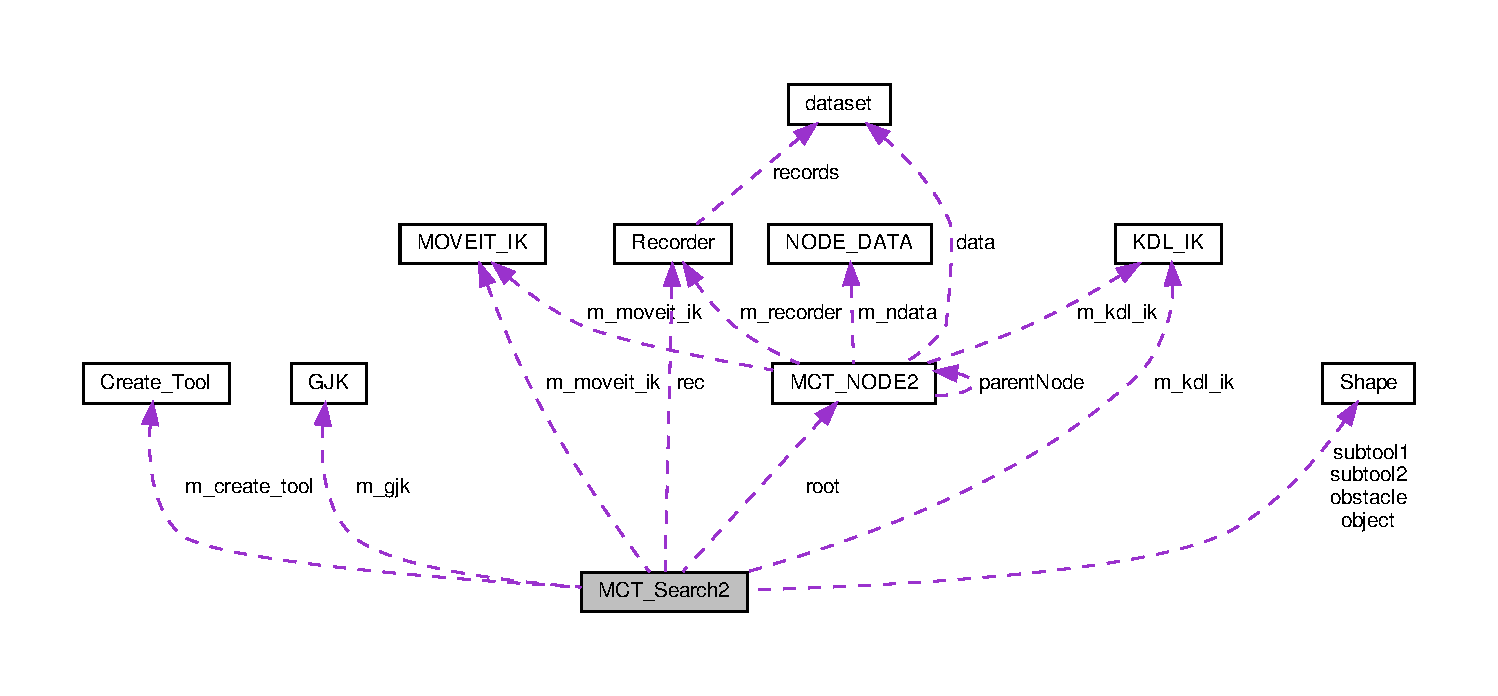
\includegraphics[width=350pt]{classMCT__Search2__coll__graph}
\end{center}
\end{figure}
\subsection*{Public Member Functions}
\begin{DoxyCompactItemize}
\item 
\mbox{\Hypertarget{classMCT__Search2_a887bedfbb47a67f217c6b661b1de9f0c}\label{classMCT__Search2_a887bedfbb47a67f217c6b661b1de9f0c}} 
\hyperlink{classMCT__Search2_a887bedfbb47a67f217c6b661b1de9f0c}{M\+C\+T\+\_\+\+Search2} ()
\begin{DoxyCompactList}\small\item\em Construct a new mct search2 object. \end{DoxyCompactList}\item 
\mbox{\Hypertarget{classMCT__Search2_aa3fe2b0773487f2eb40a91de50c55095}\label{classMCT__Search2_aa3fe2b0773487f2eb40a91de50c55095}} 
\hyperlink{classMCT__Search2_aa3fe2b0773487f2eb40a91de50c55095}{$\sim$\+M\+C\+T\+\_\+\+Search2} ()
\begin{DoxyCompactList}\small\item\em Destroy the mct search2 object. \end{DoxyCompactList}\item 
void \hyperlink{classMCT__Search2_ac3b84aa47f5eaf6323419ad1711f9ad2}{init} (\hyperlink{classCreate__Tool}{Create\+\_\+\+Tool} $\ast$create\+\_\+tool, \hyperlink{classMOVEIT__IK}{M\+O\+V\+E\+I\+T\+\_\+\+IK} $\ast$moveit\+\_\+ik, \hyperlink{classKDL__IK}{K\+D\+L\+\_\+\+IK} $\ast$kdl\+\_\+ik=N\+U\+LL, bool right=true)
\begin{DoxyCompactList}\small\item\em initialise class object \end{DoxyCompactList}\item 
void \hyperlink{classMCT__Search2_aa29f243b21264b345036ee0692bd6fb4}{init\+\_\+params} (int num\+\_\+grasp, int num\+\_\+atk\+\_\+angle, int plays=500)
\begin{DoxyCompactList}\small\item\em initialise other parameters for M\+C\+TS consideration \end{DoxyCompactList}\item 
\mbox{\Hypertarget{classMCT__Search2_ac6aa270d31c6cdb77e4783acf26e6958}\label{classMCT__Search2_ac6aa270d31c6cdb77e4783acf26e6958}} 
void \hyperlink{classMCT__Search2_ac6aa270d31c6cdb77e4783acf26e6958}{search} ()
\begin{DoxyCompactList}\small\item\em Start the M\+C\+TS search. \end{DoxyCompactList}\item 
\hyperlink{structNODE__DATA}{N\+O\+D\+E\+\_\+\+D\+A\+TA} \hyperlink{classMCT__Search2_aef5e7c7dd2c7184c021e969d6d0881a9}{set\+\_\+ndata} (int node\+\_\+idx\mbox{[}7\mbox{]}, bool cflag=false, bool sflag=false)
\begin{DoxyCompactList}\small\item\em Set the node data. \end{DoxyCompactList}\item 
vector$<$ Affine3d $>$ \hyperlink{classMCT__Search2_aa20bc38f16b562fcd6ece9605e371a30}{get\+Result} ()
\begin{DoxyCompactList}\small\item\em Get the Resulting best Path to follow to pull/push object. \end{DoxyCompactList}\item 
Affine3d \hyperlink{classMCT__Search2_a31bf88e51a19581db4957c73fc2d8a6b}{get\+Grab} ()
\begin{DoxyCompactList}\small\item\em Get the Resulting best Grab pose. \end{DoxyCompactList}\item 
double \hyperlink{classMCT__Search2_ae8ae2613e785dbcd18e861b12877c3a3}{get\+Atk\+Angle} ()
\begin{DoxyCompactList}\small\item\em Get the Resulting best attach angle of the tool to object. \end{DoxyCompactList}\item 
double \hyperlink{classMCT__Search2_a8cf59fa0e37982592de526ce450d1331}{get\+Score} ()
\begin{DoxyCompactList}\small\item\em Get the Score of the best solution. \end{DoxyCompactList}\item 
int \hyperlink{classMCT__Search2_a34c5b319ed38d852d2bbeadb80fe41e2}{get\+Via\+Pt} ()
\begin{DoxyCompactList}\small\item\em Get the Resulting best Via Point index. \end{DoxyCompactList}\item 
\mbox{\Hypertarget{classMCT__Search2_a2cbaa67d3a44d77bbf2d9d378eb38c4c}\label{classMCT__Search2_a2cbaa67d3a44d77bbf2d9d378eb38c4c}} 
void \hyperlink{classMCT__Search2_a2cbaa67d3a44d77bbf2d9d378eb38c4c}{compute\+Adjacent\+Seg} ()
\begin{DoxyCompactList}\small\item\em Compute the adjacent segment indices. \end{DoxyCompactList}\end{DoxyCompactItemize}
\subsection*{Public Attributes}
\begin{DoxyCompactItemize}
\item 
\mbox{\Hypertarget{classMCT__Search2_a777bc0064dc8c3c5c72193aa6941a075}\label{classMCT__Search2_a777bc0064dc8c3c5c72193aa6941a075}} 
int {\bfseries N\+\_\+via\+\_\+pts}
\item 
\mbox{\Hypertarget{classMCT__Search2_a2e448c5a1ba0bca78d5679dcc3083f7f}\label{classMCT__Search2_a2e448c5a1ba0bca78d5679dcc3083f7f}} 
int {\bfseries N\+\_\+intrapath\+\_\+pts}
\item 
\mbox{\Hypertarget{classMCT__Search2_ad943d84d36e9cd5bab03cef3e0511342}\label{classMCT__Search2_ad943d84d36e9cd5bab03cef3e0511342}} 
int {\bfseries N\+\_\+path\+\_\+pts}
\item 
\mbox{\Hypertarget{classMCT__Search2_a007d6e4c6bd380a763fc115bdbdd4e94}\label{classMCT__Search2_a007d6e4c6bd380a763fc115bdbdd4e94}} 
int {\bfseries max\+\_\+iter}
\item 
\mbox{\Hypertarget{classMCT__Search2_a859ecd6fc3d32b684714a5308a824a11}\label{classMCT__Search2_a859ecd6fc3d32b684714a5308a824a11}} 
int {\bfseries N\+\_\+via\+\_\+candidates}
\item 
\mbox{\Hypertarget{classMCT__Search2_acb5523a775ace0c576076c539af05ac0}\label{classMCT__Search2_acb5523a775ace0c576076c539af05ac0}} 
\hyperlink{structShape}{Shape} {\bfseries subtool1}
\item 
\mbox{\Hypertarget{classMCT__Search2_af2fad2760e627a34b632edc38d242d1b}\label{classMCT__Search2_af2fad2760e627a34b632edc38d242d1b}} 
\hyperlink{structShape}{Shape} {\bfseries subtool2}
\item 
\mbox{\Hypertarget{classMCT__Search2_a16516baf0567e019dc9a8558168bd8c8}\label{classMCT__Search2_a16516baf0567e019dc9a8558168bd8c8}} 
\hyperlink{structShape}{Shape} {\bfseries object}
\item 
\mbox{\Hypertarget{classMCT__Search2_a0805a6cbedfe230d83a2dae349463a1e}\label{classMCT__Search2_a0805a6cbedfe230d83a2dae349463a1e}} 
\hyperlink{structShape}{Shape} {\bfseries obstacle}
\item 
\mbox{\Hypertarget{classMCT__Search2_a64bb0c7c4f80003ad962fae157c4d2f0}\label{classMCT__Search2_a64bb0c7c4f80003ad962fae157c4d2f0}} 
bool {\bfseries percept\+Flag}
\item 
\mbox{\Hypertarget{classMCT__Search2_aba0d31516682de995fccb4c40ddd57cf}\label{classMCT__Search2_aba0d31516682de995fccb4c40ddd57cf}} 
vector$<$ \hyperlink{structShape}{Shape} $>$ {\bfseries tool\+\_\+pieces}
\item 
\mbox{\Hypertarget{classMCT__Search2_a443bb2f6ea5558e6f377eaf814ff9c47}\label{classMCT__Search2_a443bb2f6ea5558e6f377eaf814ff9c47}} 
bool {\bfseries obstruct\+\_\+flag}
\item 
\mbox{\Hypertarget{classMCT__Search2_a797e3e6792e0ea4b3dbf72deb1581d63}\label{classMCT__Search2_a797e3e6792e0ea4b3dbf72deb1581d63}} 
Affine3d {\bfseries T\+\_\+obj\+\_\+task}
\item 
\mbox{\Hypertarget{classMCT__Search2_aa9241908a030cb7da9ec3bae1998bb52}\label{classMCT__Search2_aa9241908a030cb7da9ec3bae1998bb52}} 
vector$<$ vector$<$ Affine3d $>$ $>$ {\bfseries all\+\_\+\+T\+\_\+world\+\_\+obj\+\_\+bb}
\item 
\mbox{\Hypertarget{classMCT__Search2_ac04dadebc1088e03c9cec4978123873d}\label{classMCT__Search2_ac04dadebc1088e03c9cec4978123873d}} 
vector$<$ vector$<$ Affine3d $>$ $>$ {\bfseries all\+\_\+\+T\+\_\+world\+\_\+obst\+\_\+bb}
\item 
\mbox{\Hypertarget{classMCT__Search2_a7047fca52d876a66623a5c7ec3976ff2}\label{classMCT__Search2_a7047fca52d876a66623a5c7ec3976ff2}} 
vector$<$ vector$<$ Affine3d $>$ $>$ {\bfseries all\+\_\+\+T\+\_\+world\+\_\+obj}
\item 
\mbox{\Hypertarget{classMCT__Search2_a47e8625c1ab998c604c52e34273653db}\label{classMCT__Search2_a47e8625c1ab998c604c52e34273653db}} 
vector$<$ vector$<$ Vector3d $>$ $>$ {\bfseries all\+\_\+move\+\_\+vec}
\item 
\mbox{\Hypertarget{classMCT__Search2_afa879d5e96b9b087611cfe109acda352}\label{classMCT__Search2_afa879d5e96b9b087611cfe109acda352}} 
vector$<$ vector$<$ Affine3d $>$ $>$ {\bfseries all\+\_\+\+T\+\_\+world\+\_\+func}
\item 
\mbox{\Hypertarget{classMCT__Search2_a43ab88db1e3c142f386e2a002e844e9d}\label{classMCT__Search2_a43ab88db1e3c142f386e2a002e844e9d}} 
vector$<$ vector$<$ Affine3d $>$ $>$ {\bfseries all\+\_\+\+T\+\_\+obj\+\_\+func}
\item 
\mbox{\Hypertarget{classMCT__Search2_ad382344b939acd4978cbe58a0de436a0}\label{classMCT__Search2_ad382344b939acd4978cbe58a0de436a0}} 
vector$<$ Affine3d $>$ {\bfseries grasp\+\_\+loci}
\item 
\mbox{\Hypertarget{classMCT__Search2_aeb10bb069e90a869860b2abd2d9c6eec}\label{classMCT__Search2_aeb10bb069e90a869860b2abd2d9c6eec}} 
double {\bfseries score}
\item 
\mbox{\Hypertarget{classMCT__Search2_ad7a1ea07377879ddc5b9fecb32b6d016}\label{classMCT__Search2_ad7a1ea07377879ddc5b9fecb32b6d016}} 
double {\bfseries value}
\item 
\mbox{\Hypertarget{classMCT__Search2_a70ec124e6107095b80c496d1c4700cb7}\label{classMCT__Search2_a70ec124e6107095b80c496d1c4700cb7}} 
vector$<$ vector$<$ int $>$ $>$ {\bfseries adj\+\_\+indices}
\end{DoxyCompactItemize}
\subsection*{Private Member Functions}
\begin{DoxyCompactItemize}
\item 
\mbox{\Hypertarget{classMCT__Search2_a3189949ccb48da64c62e0c1c9ae66f15}\label{classMCT__Search2_a3189949ccb48da64c62e0c1c9ae66f15}} 
void \hyperlink{classMCT__Search2_a3189949ccb48da64c62e0c1c9ae66f15}{monte\+\_\+carlo\+\_\+tree} ()
\begin{DoxyCompactList}\small\item\em Construct the M\+C\+TS tree. \end{DoxyCompactList}\item 
\mbox{\Hypertarget{classMCT__Search2_a5c4aa4b4b1adcb8016490074fdd653f5}\label{classMCT__Search2_a5c4aa4b4b1adcb8016490074fdd653f5}} 
void \hyperlink{classMCT__Search2_a5c4aa4b4b1adcb8016490074fdd653f5}{monte\+\_\+carlo\+\_\+search} ()
\begin{DoxyCompactList}\small\item\em Perform the M\+C\+TS search through the tree. \end{DoxyCompactList}\item 
Affine3d \hyperlink{classMCT__Search2_afabc664bbcbb6694a66c5a0b78bc0f68}{create\+\_\+affine} (double roll, double pitch, double yaw, double x, double y, double z)
\begin{DoxyCompactList}\small\item\em Create a affine object. \end{DoxyCompactList}\end{DoxyCompactItemize}
\subsection*{Private Attributes}
\begin{DoxyCompactItemize}
\item 
\mbox{\Hypertarget{classMCT__Search2_a6cef53a4e6f78582c905a8319f4a2d02}\label{classMCT__Search2_a6cef53a4e6f78582c905a8319f4a2d02}} 
bool {\bfseries m\+\_\+right}
\item 
\mbox{\Hypertarget{classMCT__Search2_ace5b703300f8e6f8e6b990300fcddcac}\label{classMCT__Search2_ace5b703300f8e6f8e6b990300fcddcac}} 
int {\bfseries Nplays}
\item 
\mbox{\Hypertarget{classMCT__Search2_afeb55503e6e8b0988804695b5cc959c5}\label{classMCT__Search2_afeb55503e6e8b0988804695b5cc959c5}} 
bool {\bfseries param\+Flag}
\item 
\mbox{\Hypertarget{classMCT__Search2_ac14215fc76a0fadbcdaf29820778ae2b}\label{classMCT__Search2_ac14215fc76a0fadbcdaf29820778ae2b}} 
\hyperlink{classCreate__Tool}{Create\+\_\+\+Tool} $\ast$ {\bfseries m\+\_\+create\+\_\+tool}
\item 
\mbox{\Hypertarget{classMCT__Search2_a16ab381b7bd1c0ef17f8d13711e8a5b1}\label{classMCT__Search2_a16ab381b7bd1c0ef17f8d13711e8a5b1}} 
\hyperlink{classMOVEIT__IK}{M\+O\+V\+E\+I\+T\+\_\+\+IK} $\ast$ {\bfseries m\+\_\+moveit\+\_\+ik}
\item 
\mbox{\Hypertarget{classMCT__Search2_afd53d98c514635059b80ff3b8a4ccd9f}\label{classMCT__Search2_afd53d98c514635059b80ff3b8a4ccd9f}} 
\hyperlink{classKDL__IK}{K\+D\+L\+\_\+\+IK} $\ast$ {\bfseries m\+\_\+kdl\+\_\+ik}
\item 
\mbox{\Hypertarget{classMCT__Search2_a38fc36400f4ea6ca7a0eba6aafe8d84f}\label{classMCT__Search2_a38fc36400f4ea6ca7a0eba6aafe8d84f}} 
\hyperlink{classGJK}{G\+JK} {\bfseries m\+\_\+gjk}
\item 
\mbox{\Hypertarget{classMCT__Search2_aed7488ccb84883ec97b6bdb82114bd0d}\label{classMCT__Search2_aed7488ccb84883ec97b6bdb82114bd0d}} 
int {\bfseries N\+\_\+grasp}
\item 
\mbox{\Hypertarget{classMCT__Search2_a8284e23248c520ad883660a7f81ecc61}\label{classMCT__Search2_a8284e23248c520ad883660a7f81ecc61}} 
int {\bfseries N\+\_\+atk\+\_\+angle}
\item 
\mbox{\Hypertarget{classMCT__Search2_a98b4050d66169ef7bdc434ebf6af9ecd}\label{classMCT__Search2_a98b4050d66169ef7bdc434ebf6af9ecd}} 
double {\bfseries atk\+\_\+angle\+\_\+step}
\item 
\mbox{\Hypertarget{classMCT__Search2_a4af66928c3894e0a3e076553218d8d39}\label{classMCT__Search2_a4af66928c3894e0a3e076553218d8d39}} 
Vector\+Xd {\bfseries atk\+\_\+angle}
\item 
\mbox{\Hypertarget{classMCT__Search2_ace3274d47de8b547410d03e3c3072ab4}\label{classMCT__Search2_ace3274d47de8b547410d03e3c3072ab4}} 
Vector\+Xd {\bfseries N\+\_\+pts}
\item 
\mbox{\Hypertarget{classMCT__Search2_ac9007c514b07e8fe9778546f33ad01f9}\label{classMCT__Search2_ac9007c514b07e8fe9778546f33ad01f9}} 
int {\bfseries N\+\_\+seg}
\item 
\mbox{\Hypertarget{classMCT__Search2_a5f725b246fd7983ad71a5ad3fa89153d}\label{classMCT__Search2_a5f725b246fd7983ad71a5ad3fa89153d}} 
vector$<$ Vector3d $>$ {\bfseries nvec\+\_\+seg}
\item 
\mbox{\Hypertarget{classMCT__Search2_ae1f12aaae410cc588bf933e60844c40d}\label{classMCT__Search2_ae1f12aaae410cc588bf933e60844c40d}} 
Vector\+Xd {\bfseries angle\+\_\+seg}
\item 
\mbox{\Hypertarget{classMCT__Search2_aa512eae7e5edbeca962a9e5376b361a5}\label{classMCT__Search2_aa512eae7e5edbeca962a9e5376b361a5}} 
vector$<$ vector$<$ Vector3d $>$ $>$ {\bfseries tool\+\_\+seg}
\item 
\mbox{\Hypertarget{classMCT__Search2_ae46e0202a8de87514af28804c9998af6}\label{classMCT__Search2_ae46e0202a8de87514af28804c9998af6}} 
\hyperlink{classMCT__NODE2}{M\+C\+T\+\_\+\+N\+O\+D\+E2} \hyperlink{classMCT__Search2_ae46e0202a8de87514af28804c9998af6}{root}
\begin{DoxyCompactList}\small\item\em the root node of the recursive mcts tree \end{DoxyCompactList}\item 
\mbox{\Hypertarget{classMCT__Search2_ad6e67e001645b1e495a6b53b6b4e16fa}\label{classMCT__Search2_ad6e67e001645b1e495a6b53b6b4e16fa}} 
double {\bfseries max\+\_\+score}
\item 
\mbox{\Hypertarget{classMCT__Search2_a28e37393acafb6585057baa91d60c2c7}\label{classMCT__Search2_a28e37393acafb6585057baa91d60c2c7}} 
vector$<$ int $>$ {\bfseries best}
\item 
\mbox{\Hypertarget{classMCT__Search2_a37113270700238ba6e3b6d3127d059b9}\label{classMCT__Search2_a37113270700238ba6e3b6d3127d059b9}} 
vector$<$ Affine3d $>$ {\bfseries result\+\_\+\+T\+\_\+real\+\_\+grasp}
\item 
\mbox{\Hypertarget{classMCT__Search2_a8d8d1889224c49076725d99d218ff430}\label{classMCT__Search2_a8d8d1889224c49076725d99d218ff430}} 
Affine3d {\bfseries result\+\_\+grab\+\_\+pos}
\item 
\mbox{\Hypertarget{classMCT__Search2_a9b29cb64bd967d71b0ef4a56d473a0cb}\label{classMCT__Search2_a9b29cb64bd967d71b0ef4a56d473a0cb}} 
double {\bfseries result\+\_\+atk\+\_\+angle}
\item 
\mbox{\Hypertarget{classMCT__Search2_a3c6905ec9d8bddb1e1055cd01d11286f}\label{classMCT__Search2_a3c6905ec9d8bddb1e1055cd01d11286f}} 
int {\bfseries result\+\_\+via\+\_\+pt\+\_\+index}
\item 
\mbox{\Hypertarget{classMCT__Search2_a93ad76aeefbab8848287f334e1494c46}\label{classMCT__Search2_a93ad76aeefbab8848287f334e1494c46}} 
\hyperlink{classRecorder}{Recorder} \hyperlink{classMCT__Search2_a93ad76aeefbab8848287f334e1494c46}{rec}
\begin{DoxyCompactList}\small\item\em logger \end{DoxyCompactList}\end{DoxyCompactItemize}


\subsection{Detailed Description}
Class object to perform monte carlo tree search algorithm recursive function, optimisation and memory save version 2.\+0. 

\subsection{Member Function Documentation}
\mbox{\Hypertarget{classMCT__Search2_afabc664bbcbb6694a66c5a0b78bc0f68}\label{classMCT__Search2_afabc664bbcbb6694a66c5a0b78bc0f68}} 
\index{M\+C\+T\+\_\+\+Search2@{M\+C\+T\+\_\+\+Search2}!create\+\_\+affine@{create\+\_\+affine}}
\index{create\+\_\+affine@{create\+\_\+affine}!M\+C\+T\+\_\+\+Search2@{M\+C\+T\+\_\+\+Search2}}
\subsubsection{\texorpdfstring{create\+\_\+affine()}{create\_affine()}}
{\footnotesize\ttfamily Affine3d M\+C\+T\+\_\+\+Search2\+::create\+\_\+affine (\begin{DoxyParamCaption}\item[{double}]{roll,  }\item[{double}]{pitch,  }\item[{double}]{yaw,  }\item[{double}]{x,  }\item[{double}]{y,  }\item[{double}]{z }\end{DoxyParamCaption})\hspace{0.3cm}{\ttfamily [private]}}



Create a affine object. 


\begin{DoxyParams}{Parameters}
{\em roll} & angle in radian \\
\hline
{\em pitch} & angle in radian \\
\hline
{\em yaw} & angle in radian \\
\hline
{\em x} & translation in x \\
\hline
{\em y} & translation in y \\
\hline
{\em z} & translation in z \\
\hline
\end{DoxyParams}
\begin{DoxyReturn}{Returns}
Affine3d eigen affine matrix 
\end{DoxyReturn}
\mbox{\Hypertarget{classMCT__Search2_ae8ae2613e785dbcd18e861b12877c3a3}\label{classMCT__Search2_ae8ae2613e785dbcd18e861b12877c3a3}} 
\index{M\+C\+T\+\_\+\+Search2@{M\+C\+T\+\_\+\+Search2}!get\+Atk\+Angle@{get\+Atk\+Angle}}
\index{get\+Atk\+Angle@{get\+Atk\+Angle}!M\+C\+T\+\_\+\+Search2@{M\+C\+T\+\_\+\+Search2}}
\subsubsection{\texorpdfstring{get\+Atk\+Angle()}{getAtkAngle()}}
{\footnotesize\ttfamily double M\+C\+T\+\_\+\+Search2\+::get\+Atk\+Angle (\begin{DoxyParamCaption}{ }\end{DoxyParamCaption})\hspace{0.3cm}{\ttfamily [inline]}}



Get the Resulting best attach angle of the tool to object. 

\begin{DoxyReturn}{Returns}
double angle 
\end{DoxyReturn}
\mbox{\Hypertarget{classMCT__Search2_a31bf88e51a19581db4957c73fc2d8a6b}\label{classMCT__Search2_a31bf88e51a19581db4957c73fc2d8a6b}} 
\index{M\+C\+T\+\_\+\+Search2@{M\+C\+T\+\_\+\+Search2}!get\+Grab@{get\+Grab}}
\index{get\+Grab@{get\+Grab}!M\+C\+T\+\_\+\+Search2@{M\+C\+T\+\_\+\+Search2}}
\subsubsection{\texorpdfstring{get\+Grab()}{getGrab()}}
{\footnotesize\ttfamily Affine3d M\+C\+T\+\_\+\+Search2\+::get\+Grab (\begin{DoxyParamCaption}{ }\end{DoxyParamCaption})\hspace{0.3cm}{\ttfamily [inline]}}



Get the Resulting best Grab pose. 

\begin{DoxyReturn}{Returns}
Affine3d grab pose 
\end{DoxyReturn}
\mbox{\Hypertarget{classMCT__Search2_aa20bc38f16b562fcd6ece9605e371a30}\label{classMCT__Search2_aa20bc38f16b562fcd6ece9605e371a30}} 
\index{M\+C\+T\+\_\+\+Search2@{M\+C\+T\+\_\+\+Search2}!get\+Result@{get\+Result}}
\index{get\+Result@{get\+Result}!M\+C\+T\+\_\+\+Search2@{M\+C\+T\+\_\+\+Search2}}
\subsubsection{\texorpdfstring{get\+Result()}{getResult()}}
{\footnotesize\ttfamily vector$<$ Affine3d $>$ M\+C\+T\+\_\+\+Search2\+::get\+Result (\begin{DoxyParamCaption}{ }\end{DoxyParamCaption})\hspace{0.3cm}{\ttfamily [inline]}}



Get the Resulting best Path to follow to pull/push object. 

\begin{DoxyReturn}{Returns}
vector$<$ Affine3d $>$ best path 
\end{DoxyReturn}
\mbox{\Hypertarget{classMCT__Search2_a8cf59fa0e37982592de526ce450d1331}\label{classMCT__Search2_a8cf59fa0e37982592de526ce450d1331}} 
\index{M\+C\+T\+\_\+\+Search2@{M\+C\+T\+\_\+\+Search2}!get\+Score@{get\+Score}}
\index{get\+Score@{get\+Score}!M\+C\+T\+\_\+\+Search2@{M\+C\+T\+\_\+\+Search2}}
\subsubsection{\texorpdfstring{get\+Score()}{getScore()}}
{\footnotesize\ttfamily double M\+C\+T\+\_\+\+Search2\+::get\+Score (\begin{DoxyParamCaption}{ }\end{DoxyParamCaption})\hspace{0.3cm}{\ttfamily [inline]}}



Get the Score of the best solution. 

\begin{DoxyReturn}{Returns}
double score 
\end{DoxyReturn}
\mbox{\Hypertarget{classMCT__Search2_a34c5b319ed38d852d2bbeadb80fe41e2}\label{classMCT__Search2_a34c5b319ed38d852d2bbeadb80fe41e2}} 
\index{M\+C\+T\+\_\+\+Search2@{M\+C\+T\+\_\+\+Search2}!get\+Via\+Pt@{get\+Via\+Pt}}
\index{get\+Via\+Pt@{get\+Via\+Pt}!M\+C\+T\+\_\+\+Search2@{M\+C\+T\+\_\+\+Search2}}
\subsubsection{\texorpdfstring{get\+Via\+Pt()}{getViaPt()}}
{\footnotesize\ttfamily int M\+C\+T\+\_\+\+Search2\+::get\+Via\+Pt (\begin{DoxyParamCaption}{ }\end{DoxyParamCaption})\hspace{0.3cm}{\ttfamily [inline]}}



Get the Resulting best Via Point index. 

\begin{DoxyReturn}{Returns}
int index of the best via point 
\end{DoxyReturn}
\mbox{\Hypertarget{classMCT__Search2_ac3b84aa47f5eaf6323419ad1711f9ad2}\label{classMCT__Search2_ac3b84aa47f5eaf6323419ad1711f9ad2}} 
\index{M\+C\+T\+\_\+\+Search2@{M\+C\+T\+\_\+\+Search2}!init@{init}}
\index{init@{init}!M\+C\+T\+\_\+\+Search2@{M\+C\+T\+\_\+\+Search2}}
\subsubsection{\texorpdfstring{init()}{init()}}
{\footnotesize\ttfamily void M\+C\+T\+\_\+\+Search2\+::init (\begin{DoxyParamCaption}\item[{\hyperlink{classCreate__Tool}{Create\+\_\+\+Tool} $\ast$}]{create\+\_\+tool,  }\item[{\hyperlink{classMOVEIT__IK}{M\+O\+V\+E\+I\+T\+\_\+\+IK} $\ast$}]{moveit\+\_\+ik,  }\item[{\hyperlink{classKDL__IK}{K\+D\+L\+\_\+\+IK} $\ast$}]{kdl\+\_\+ik = {\ttfamily NULL},  }\item[{bool}]{right = {\ttfamily true} }\end{DoxyParamCaption})}



initialise class object 


\begin{DoxyParams}{Parameters}
{\em create\+\_\+tool} & pointer to create\+\_\+tool class object \\
\hline
{\em moveit\+\_\+ik} & pointer to moveit IK solver object \\
\hline
{\em kdl\+\_\+ik} & pointer to kdl IK solver object \\
\hline
{\em right} & which arm, true=right, false=left \\
\hline
\end{DoxyParams}
\mbox{\Hypertarget{classMCT__Search2_aa29f243b21264b345036ee0692bd6fb4}\label{classMCT__Search2_aa29f243b21264b345036ee0692bd6fb4}} 
\index{M\+C\+T\+\_\+\+Search2@{M\+C\+T\+\_\+\+Search2}!init\+\_\+params@{init\+\_\+params}}
\index{init\+\_\+params@{init\+\_\+params}!M\+C\+T\+\_\+\+Search2@{M\+C\+T\+\_\+\+Search2}}
\subsubsection{\texorpdfstring{init\+\_\+params()}{init\_params()}}
{\footnotesize\ttfamily void M\+C\+T\+\_\+\+Search2\+::init\+\_\+params (\begin{DoxyParamCaption}\item[{int}]{num\+\_\+grasp,  }\item[{int}]{num\+\_\+atk\+\_\+angle,  }\item[{int}]{plays = {\ttfamily 500} }\end{DoxyParamCaption})}



initialise other parameters for M\+C\+TS consideration 


\begin{DoxyParams}{Parameters}
{\em num\+\_\+grasp} & number of grasping pose to interpolate \\
\hline
{\em num\+\_\+atk\+\_\+angle} & the attack angle of the tool \\
\hline
{\em plays} & number of search iterations \\
\hline
\end{DoxyParams}
\mbox{\Hypertarget{classMCT__Search2_aef5e7c7dd2c7184c021e969d6d0881a9}\label{classMCT__Search2_aef5e7c7dd2c7184c021e969d6d0881a9}} 
\index{M\+C\+T\+\_\+\+Search2@{M\+C\+T\+\_\+\+Search2}!set\+\_\+ndata@{set\+\_\+ndata}}
\index{set\+\_\+ndata@{set\+\_\+ndata}!M\+C\+T\+\_\+\+Search2@{M\+C\+T\+\_\+\+Search2}}
\subsubsection{\texorpdfstring{set\+\_\+ndata()}{set\_ndata()}}
{\footnotesize\ttfamily \hyperlink{structNODE__DATA}{N\+O\+D\+E\+\_\+\+D\+A\+TA} M\+C\+T\+\_\+\+Search2\+::set\+\_\+ndata (\begin{DoxyParamCaption}\item[{int}]{node\+\_\+idx\mbox{[}7\mbox{]},  }\item[{bool}]{cflag = {\ttfamily false},  }\item[{bool}]{sflag = {\ttfamily false} }\end{DoxyParamCaption})}



Set the node data. 


\begin{DoxyParams}{Parameters}
{\em node\+\_\+idx} & node index \\
\hline
{\em cflag} & is there a collision object? \\
\hline
{\em sflag} & is it a small segment? \\
\hline
\end{DoxyParams}
\begin{DoxyReturn}{Returns}
\hyperlink{structNODE__DATA}{N\+O\+D\+E\+\_\+\+D\+A\+TA} 
\end{DoxyReturn}


The documentation for this class was generated from the following files\+:\begin{DoxyCompactItemize}
\item 
/home/samuel/\+Desktop/toolcog\+\_\+ws/montecarlo/include/tool\+\_\+expt/\hyperlink{search2_8h}{search2.\+h}\item 
/home/samuel/\+Desktop/toolcog\+\_\+ws/montecarlo/src/search2.\+cpp\end{DoxyCompactItemize}

\hypertarget{classmove__fingers_1_1MoveFingers}{}\section{move\+\_\+fingers.\+Move\+Fingers Class Reference}
\label{classmove__fingers_1_1MoveFingers}\index{move\+\_\+fingers.\+Move\+Fingers@{move\+\_\+fingers.\+Move\+Fingers}}
\subsection*{Public Member Functions}
\begin{DoxyCompactItemize}
\item 
\mbox{\Hypertarget{classmove__fingers_1_1MoveFingers_ac26eb41f09acd1d29f395a5649b4403f}\label{classmove__fingers_1_1MoveFingers_ac26eb41f09acd1d29f395a5649b4403f}} 
def {\bfseries \+\_\+\+\_\+init\+\_\+\+\_\+} (self)
\item 
\mbox{\Hypertarget{classmove__fingers_1_1MoveFingers_a999e4869c8a5bf42e29d490f67a82516}\label{classmove__fingers_1_1MoveFingers_a999e4869c8a5bf42e29d490f67a82516}} 
def {\bfseries open\+Fingers} (self)
\item 
\mbox{\Hypertarget{classmove__fingers_1_1MoveFingers_ab8f25216fbc15f7dec7ee0730a8051ec}\label{classmove__fingers_1_1MoveFingers_ab8f25216fbc15f7dec7ee0730a8051ec}} 
def {\bfseries open\+Trigger} (self)
\item 
\mbox{\Hypertarget{classmove__fingers_1_1MoveFingers_ac43323a6d04eba138aa94ec0d4cfcc4d}\label{classmove__fingers_1_1MoveFingers_ac43323a6d04eba138aa94ec0d4cfcc4d}} 
def {\bfseries close\+Fingers} (self)
\item 
\mbox{\Hypertarget{classmove__fingers_1_1MoveFingers_a3c7a6505ef6858d5ad59355a8f195a10}\label{classmove__fingers_1_1MoveFingers_a3c7a6505ef6858d5ad59355a8f195a10}} 
def {\bfseries close\+Trigger} (self)
\item 
\mbox{\Hypertarget{classmove__fingers_1_1MoveFingers_ad7e2c7ae218593a274042a772464ceea}\label{classmove__fingers_1_1MoveFingers_ad7e2c7ae218593a274042a772464ceea}} 
def {\bfseries stop\+Fingers} (self)
\end{DoxyCompactItemize}
\subsection*{Public Attributes}
\begin{DoxyCompactItemize}
\item 
\mbox{\Hypertarget{classmove__fingers_1_1MoveFingers_aa4da3af73d110c5dda41c6afcdad0b8d}\label{classmove__fingers_1_1MoveFingers_aa4da3af73d110c5dda41c6afcdad0b8d}} 
{\bfseries pub}
\end{DoxyCompactItemize}


The documentation for this class was generated from the following file\+:\begin{DoxyCompactItemize}
\item 
/home/samuel/\+Desktop/toolcog\+\_\+ws/montecarlo/python/move\+\_\+fingers.\+py\end{DoxyCompactItemize}

\hypertarget{classMOVEIT__IK}{}\section{M\+O\+V\+E\+I\+T\+\_\+\+IK Class Reference}
\label{classMOVEIT__IK}\index{M\+O\+V\+E\+I\+T\+\_\+\+IK@{M\+O\+V\+E\+I\+T\+\_\+\+IK}}


ik solver using moveit for node.\+m R\+OS library usage, moveit kinematics setup class to quickly solve IK  




{\ttfamily \#include $<$moveit\+\_\+ik.\+h$>$}

\subsection*{Public Member Functions}
\begin{DoxyCompactItemize}
\item 
\mbox{\Hypertarget{classMOVEIT__IK_a8f6dd02b0c1c1c4528552fdcdb8af1e1}\label{classMOVEIT__IK_a8f6dd02b0c1c1c4528552fdcdb8af1e1}} 
\hyperlink{classMOVEIT__IK_a8f6dd02b0c1c1c4528552fdcdb8af1e1}{M\+O\+V\+E\+I\+T\+\_\+\+IK} ()
\begin{DoxyCompactList}\small\item\em Construct a new moveit ik object. \end{DoxyCompactList}\item 
\mbox{\Hypertarget{classMOVEIT__IK_aff4d253c101968b8e756e9f179270109}\label{classMOVEIT__IK_aff4d253c101968b8e756e9f179270109}} 
\hyperlink{classMOVEIT__IK_aff4d253c101968b8e756e9f179270109}{$\sim$\+M\+O\+V\+E\+I\+T\+\_\+\+IK} ()
\begin{DoxyCompactList}\small\item\em Destroy the moveit ik object. \end{DoxyCompactList}\item 
void \hyperlink{classMOVEIT__IK_a93f8e535f8fbbe54100d8eecdd2ee6e4}{init} (bool right=true)
\begin{DoxyCompactList}\small\item\em initialise moveit ik object moveit requires to load the robot model as a moveit kinematics model the planning scene will update using this kinematics model ik is solved by setting this kinematics model with the given joint values, and returning the solution of its end-\/effector in cartesian space \end{DoxyCompactList}\item 
void \hyperlink{classMOVEIT__IK_af5b81c18b576ae1371ddc866061df1d5}{init\+\_\+home} (vector$<$ double $>$ joint\+\_\+values)
\begin{DoxyCompactList}\small\item\em perform forward kinematics (FK) and store the position of given joint values as the home position \end{DoxyCompactList}\item 
bool \hyperlink{classMOVEIT__IK_a790708eba19044f34e00c2e78998ff09}{ik\+\_\+solve} (Affine3d target\+\_\+\+KS)
\begin{DoxyCompactList}\small\item\em Function to solve the IK for the given target pose. \end{DoxyCompactList}\item 
void \hyperlink{classMOVEIT__IK_a0bdc6f6a1cefeaad6651495c463dd6ed}{update\+\_\+arm} (vector$<$ double $>$ arm\+\_\+joint\+\_\+values)
\begin{DoxyCompactList}\small\item\em update the kinematic state of the arm with the given joint values \end{DoxyCompactList}\item 
void \hyperlink{classMOVEIT__IK_a1399d0e0159b8ed7af938116fee6dc93}{update} (vector$<$ double $>$ joint\+\_\+values)
\begin{DoxyCompactList}\small\item\em update the kinematic state of the arm+torso with the given joint values \end{DoxyCompactList}\item 
\mbox{\Hypertarget{classMOVEIT__IK_af059baeee7ac1bdfc109e775f710380a}\label{classMOVEIT__IK_af059baeee7ac1bdfc109e775f710380a}} 
void \hyperlink{classMOVEIT__IK_af059baeee7ac1bdfc109e775f710380a}{reset} ()
\begin{DoxyCompactList}\small\item\em reset both the arm and torso kinematics model to the \textquotesingle{}Home\textquotesingle{} position \end{DoxyCompactList}\item 
Matrix\+Xd \hyperlink{classMOVEIT__IK_a0086f93313ee7036d8897d6156b1395b}{jacobian\+\_\+solve} ()
\begin{DoxyCompactList}\small\item\em compute the jacobian for the kinematics model \end{DoxyCompactList}\item 
\mbox{\Hypertarget{classMOVEIT__IK_a1cd828f223bc110073993c8df6b9a561}\label{classMOVEIT__IK_a1cd828f223bc110073993c8df6b9a561}} 
void \hyperlink{classMOVEIT__IK_a1cd828f223bc110073993c8df6b9a561}{get\+Joint\+Limits} ()
\begin{DoxyCompactList}\small\item\em Get the Joint Limits form the moveit kinematics model must be stated in the urdf. \end{DoxyCompactList}\item 
bool \hyperlink{classMOVEIT__IK_aecc7b36de162360f11ad460d3fb2321c}{check\+Joint\+Limits} ()
\begin{DoxyCompactList}\small\item\em check if joint values of IK solution exceeds software joint limits Sometimes kinematics model exceeds acceptable joint limits (double-\/check to eliminate bug) \end{DoxyCompactList}\end{DoxyCompactItemize}
\subsection*{Public Attributes}
\begin{DoxyCompactItemize}
\item 
\mbox{\Hypertarget{classMOVEIT__IK_a96a7cdcec1cc5495fbefd8f7d0fb2abd}\label{classMOVEIT__IK_a96a7cdcec1cc5495fbefd8f7d0fb2abd}} 
vector$<$ double $>$ \hyperlink{classMOVEIT__IK_a96a7cdcec1cc5495fbefd8f7d0fb2abd}{max\+\_\+limit}
\begin{DoxyCompactList}\small\item\em store the maximum joint limit \end{DoxyCompactList}\item 
\mbox{\Hypertarget{classMOVEIT__IK_acf4cefec4cf6a6a9f2c686e72ac5ca88}\label{classMOVEIT__IK_acf4cefec4cf6a6a9f2c686e72ac5ca88}} 
vector$<$ double $>$ \hyperlink{classMOVEIT__IK_acf4cefec4cf6a6a9f2c686e72ac5ca88}{min\+\_\+limit}
\begin{DoxyCompactList}\small\item\em store the minimum joint limit \end{DoxyCompactList}\item 
\mbox{\Hypertarget{classMOVEIT__IK_a9a56827e336f026573086de4924f1b79}\label{classMOVEIT__IK_a9a56827e336f026573086de4924f1b79}} 
vector$<$ double $>$ \hyperlink{classMOVEIT__IK_a9a56827e336f026573086de4924f1b79}{desired\+\_\+arm\+\_\+values}
\begin{DoxyCompactList}\small\item\em store the desired joint values for the arm \end{DoxyCompactList}\item 
\mbox{\Hypertarget{classMOVEIT__IK_a4dd561e5e04d724bd7bbe5bd68f1941c}\label{classMOVEIT__IK_a4dd561e5e04d724bd7bbe5bd68f1941c}} 
vector$<$ double $>$ \hyperlink{classMOVEIT__IK_a4dd561e5e04d724bd7bbe5bd68f1941c}{desired\+\_\+joint\+\_\+values}
\begin{DoxyCompactList}\small\item\em store the desired joint values for the arm+torso \end{DoxyCompactList}\item 
\mbox{\Hypertarget{classMOVEIT__IK_a142336a7c121f66031ebfc760cb16f00}\label{classMOVEIT__IK_a142336a7c121f66031ebfc760cb16f00}} 
robot\+\_\+model\+::\+Robot\+Model\+Ptr \hyperlink{classMOVEIT__IK_a142336a7c121f66031ebfc760cb16f00}{kinematic\+\_\+model}
\begin{DoxyCompactList}\small\item\em store moveit kinematics model object \end{DoxyCompactList}\item 
\mbox{\Hypertarget{classMOVEIT__IK_a30a052ada12389671b0042507d8eb9b7}\label{classMOVEIT__IK_a30a052ada12389671b0042507d8eb9b7}} 
robot\+\_\+state\+::\+Robot\+State\+Ptr \hyperlink{classMOVEIT__IK_a30a052ada12389671b0042507d8eb9b7}{kinematic\+\_\+state}
\begin{DoxyCompactList}\small\item\em store moveit kinematics state object \end{DoxyCompactList}\end{DoxyCompactItemize}
\subsection*{Private Attributes}
\begin{DoxyCompactItemize}
\item 
\mbox{\Hypertarget{classMOVEIT__IK_ad31a54376790256d55754c1d1a0c78f7}\label{classMOVEIT__IK_ad31a54376790256d55754c1d1a0c78f7}} 
planning\+\_\+scene\+::\+Planning\+Scene\+Ptr \hyperlink{classMOVEIT__IK_ad31a54376790256d55754c1d1a0c78f7}{planning\+\_\+scene\+\_\+}
\begin{DoxyCompactList}\small\item\em store a planning scene object \end{DoxyCompactList}\item 
\mbox{\Hypertarget{classMOVEIT__IK_aa720def30962972d30dd6e0281683484}\label{classMOVEIT__IK_aa720def30962972d30dd6e0281683484}} 
std\+::vector$<$ std\+::string $>$ \hyperlink{classMOVEIT__IK_aa720def30962972d30dd6e0281683484}{mv\+\_\+joint\+\_\+names}
\begin{DoxyCompactList}\small\item\em store the joint names \end{DoxyCompactList}\item 
\mbox{\Hypertarget{classMOVEIT__IK_a0222dac5b064cbff21ab98601bceadd1}\label{classMOVEIT__IK_a0222dac5b064cbff21ab98601bceadd1}} 
robot\+\_\+state\+::\+Joint\+Model\+Group $\ast$ \hyperlink{classMOVEIT__IK_a0222dac5b064cbff21ab98601bceadd1}{joint\+\_\+model\+\_\+group}
\begin{DoxyCompactList}\small\item\em pointer to robot joint model group \end{DoxyCompactList}\item 
\mbox{\Hypertarget{classMOVEIT__IK_a11e1731426f82e3d6e17dcded5b93946}\label{classMOVEIT__IK_a11e1731426f82e3d6e17dcded5b93946}} 
std\+::vector$<$ std\+::string $>$ \hyperlink{classMOVEIT__IK_a11e1731426f82e3d6e17dcded5b93946}{arm\+\_\+joint\+\_\+names}
\begin{DoxyCompactList}\small\item\em joint names for the arm \end{DoxyCompactList}\item 
\mbox{\Hypertarget{classMOVEIT__IK_a915a894a8c31ed440b5bde7dfb11b972}\label{classMOVEIT__IK_a915a894a8c31ed440b5bde7dfb11b972}} 
robot\+\_\+state\+::\+Joint\+Model\+Group $\ast$ \hyperlink{classMOVEIT__IK_a915a894a8c31ed440b5bde7dfb11b972}{arm\+\_\+model\+\_\+group}
\begin{DoxyCompactList}\small\item\em pointer to the moveit arm group \end{DoxyCompactList}\item 
\mbox{\Hypertarget{classMOVEIT__IK_a54fb3f15c72e83b37c1aff9bb48dddd8}\label{classMOVEIT__IK_a54fb3f15c72e83b37c1aff9bb48dddd8}} 
std\+::vector$<$ double $>$ \hyperlink{classMOVEIT__IK_a54fb3f15c72e83b37c1aff9bb48dddd8}{home\+\_\+arm}
\begin{DoxyCompactList}\small\item\em store joint values for the arm\textquotesingle{}s \textquotesingle{}Home\textquotesingle{} pose \end{DoxyCompactList}\item 
\mbox{\Hypertarget{classMOVEIT__IK_a40b5380aca0f43ac807a88a521c62eaf}\label{classMOVEIT__IK_a40b5380aca0f43ac807a88a521c62eaf}} 
std\+::vector$<$ double $>$ \hyperlink{classMOVEIT__IK_a40b5380aca0f43ac807a88a521c62eaf}{home}
\begin{DoxyCompactList}\small\item\em store joint values for the arm+torso\textquotesingle{}s \textquotesingle{}Home\textquotesingle{} pose \end{DoxyCompactList}\item 
\mbox{\Hypertarget{classMOVEIT__IK_a189c9c745418ad99ab7236cabec0155a}\label{classMOVEIT__IK_a189c9c745418ad99ab7236cabec0155a}} 
vector$<$ moveit\+\_\+msgs\+::\+Joint\+Limits $>$ $\ast$ \hyperlink{classMOVEIT__IK_a189c9c745418ad99ab7236cabec0155a}{jvl}
\begin{DoxyCompactList}\small\item\em pointer to a set of joint limits \end{DoxyCompactList}\end{DoxyCompactItemize}


\subsection{Detailed Description}
ik solver using moveit for node.\+m R\+OS library usage, moveit kinematics setup class to quickly solve IK 

\subsection{Member Function Documentation}
\mbox{\Hypertarget{classMOVEIT__IK_aecc7b36de162360f11ad460d3fb2321c}\label{classMOVEIT__IK_aecc7b36de162360f11ad460d3fb2321c}} 
\index{M\+O\+V\+E\+I\+T\+\_\+\+IK@{M\+O\+V\+E\+I\+T\+\_\+\+IK}!check\+Joint\+Limits@{check\+Joint\+Limits}}
\index{check\+Joint\+Limits@{check\+Joint\+Limits}!M\+O\+V\+E\+I\+T\+\_\+\+IK@{M\+O\+V\+E\+I\+T\+\_\+\+IK}}
\subsubsection{\texorpdfstring{check\+Joint\+Limits()}{checkJointLimits()}}
{\footnotesize\ttfamily bool M\+O\+V\+E\+I\+T\+\_\+\+I\+K\+::check\+Joint\+Limits (\begin{DoxyParamCaption}{ }\end{DoxyParamCaption})\hspace{0.3cm}{\ttfamily [inline]}}



check if joint values of IK solution exceeds software joint limits Sometimes kinematics model exceeds acceptable joint limits (double-\/check to eliminate bug) 

\begin{DoxyReturn}{Returns}
true solution within joint limits 

false exceeds the joint limits = reject solution 
\end{DoxyReturn}
\mbox{\Hypertarget{classMOVEIT__IK_a790708eba19044f34e00c2e78998ff09}\label{classMOVEIT__IK_a790708eba19044f34e00c2e78998ff09}} 
\index{M\+O\+V\+E\+I\+T\+\_\+\+IK@{M\+O\+V\+E\+I\+T\+\_\+\+IK}!ik\+\_\+solve@{ik\+\_\+solve}}
\index{ik\+\_\+solve@{ik\+\_\+solve}!M\+O\+V\+E\+I\+T\+\_\+\+IK@{M\+O\+V\+E\+I\+T\+\_\+\+IK}}
\subsubsection{\texorpdfstring{ik\+\_\+solve()}{ik\_solve()}}
{\footnotesize\ttfamily bool M\+O\+V\+E\+I\+T\+\_\+\+I\+K\+::ik\+\_\+solve (\begin{DoxyParamCaption}\item[{Affine3d}]{target\+\_\+\+KS }\end{DoxyParamCaption})\hspace{0.3cm}{\ttfamily [inline]}}



Function to solve the IK for the given target pose. 


\begin{DoxyParams}{Parameters}
{\em target\+\_\+\+KS} & Affine matrix for the target \\
\hline
\end{DoxyParams}
\begin{DoxyReturn}{Returns}
true IK solved successfully 

false error encountered 
\end{DoxyReturn}
\mbox{\Hypertarget{classMOVEIT__IK_a93f8e535f8fbbe54100d8eecdd2ee6e4}\label{classMOVEIT__IK_a93f8e535f8fbbe54100d8eecdd2ee6e4}} 
\index{M\+O\+V\+E\+I\+T\+\_\+\+IK@{M\+O\+V\+E\+I\+T\+\_\+\+IK}!init@{init}}
\index{init@{init}!M\+O\+V\+E\+I\+T\+\_\+\+IK@{M\+O\+V\+E\+I\+T\+\_\+\+IK}}
\subsubsection{\texorpdfstring{init()}{init()}}
{\footnotesize\ttfamily void M\+O\+V\+E\+I\+T\+\_\+\+I\+K\+::init (\begin{DoxyParamCaption}\item[{bool}]{right = {\ttfamily true} }\end{DoxyParamCaption})\hspace{0.3cm}{\ttfamily [inline]}}



initialise moveit ik object moveit requires to load the robot model as a moveit kinematics model the planning scene will update using this kinematics model ik is solved by setting this kinematics model with the given joint values, and returning the solution of its end-\/effector in cartesian space 


\begin{DoxyParams}{Parameters}
{\em right} & true = right arm of Olivia, false = left arm of Olivia \\
\hline
\end{DoxyParams}
\mbox{\Hypertarget{classMOVEIT__IK_af5b81c18b576ae1371ddc866061df1d5}\label{classMOVEIT__IK_af5b81c18b576ae1371ddc866061df1d5}} 
\index{M\+O\+V\+E\+I\+T\+\_\+\+IK@{M\+O\+V\+E\+I\+T\+\_\+\+IK}!init\+\_\+home@{init\+\_\+home}}
\index{init\+\_\+home@{init\+\_\+home}!M\+O\+V\+E\+I\+T\+\_\+\+IK@{M\+O\+V\+E\+I\+T\+\_\+\+IK}}
\subsubsection{\texorpdfstring{init\+\_\+home()}{init\_home()}}
{\footnotesize\ttfamily void M\+O\+V\+E\+I\+T\+\_\+\+I\+K\+::init\+\_\+home (\begin{DoxyParamCaption}\item[{vector$<$ double $>$}]{joint\+\_\+values }\end{DoxyParamCaption})\hspace{0.3cm}{\ttfamily [inline]}}



perform forward kinematics (FK) and store the position of given joint values as the home position 


\begin{DoxyParams}{Parameters}
{\em joint\+\_\+values} & \\
\hline
\end{DoxyParams}
\mbox{\Hypertarget{classMOVEIT__IK_a0086f93313ee7036d8897d6156b1395b}\label{classMOVEIT__IK_a0086f93313ee7036d8897d6156b1395b}} 
\index{M\+O\+V\+E\+I\+T\+\_\+\+IK@{M\+O\+V\+E\+I\+T\+\_\+\+IK}!jacobian\+\_\+solve@{jacobian\+\_\+solve}}
\index{jacobian\+\_\+solve@{jacobian\+\_\+solve}!M\+O\+V\+E\+I\+T\+\_\+\+IK@{M\+O\+V\+E\+I\+T\+\_\+\+IK}}
\subsubsection{\texorpdfstring{jacobian\+\_\+solve()}{jacobian\_solve()}}
{\footnotesize\ttfamily Matrix\+Xd M\+O\+V\+E\+I\+T\+\_\+\+I\+K\+::jacobian\+\_\+solve (\begin{DoxyParamCaption}{ }\end{DoxyParamCaption})\hspace{0.3cm}{\ttfamily [inline]}}



compute the jacobian for the kinematics model 

\begin{DoxyReturn}{Returns}
Matrix\+Xd jacobian matrix 
\end{DoxyReturn}
\mbox{\Hypertarget{classMOVEIT__IK_a1399d0e0159b8ed7af938116fee6dc93}\label{classMOVEIT__IK_a1399d0e0159b8ed7af938116fee6dc93}} 
\index{M\+O\+V\+E\+I\+T\+\_\+\+IK@{M\+O\+V\+E\+I\+T\+\_\+\+IK}!update@{update}}
\index{update@{update}!M\+O\+V\+E\+I\+T\+\_\+\+IK@{M\+O\+V\+E\+I\+T\+\_\+\+IK}}
\subsubsection{\texorpdfstring{update()}{update()}}
{\footnotesize\ttfamily void M\+O\+V\+E\+I\+T\+\_\+\+I\+K\+::update (\begin{DoxyParamCaption}\item[{vector$<$ double $>$}]{joint\+\_\+values }\end{DoxyParamCaption})\hspace{0.3cm}{\ttfamily [inline]}}



update the kinematic state of the arm+torso with the given joint values 


\begin{DoxyParams}{Parameters}
{\em joint\+\_\+values} & input joint values for the olivia arm+torso \\
\hline
\end{DoxyParams}
\mbox{\Hypertarget{classMOVEIT__IK_a0bdc6f6a1cefeaad6651495c463dd6ed}\label{classMOVEIT__IK_a0bdc6f6a1cefeaad6651495c463dd6ed}} 
\index{M\+O\+V\+E\+I\+T\+\_\+\+IK@{M\+O\+V\+E\+I\+T\+\_\+\+IK}!update\+\_\+arm@{update\+\_\+arm}}
\index{update\+\_\+arm@{update\+\_\+arm}!M\+O\+V\+E\+I\+T\+\_\+\+IK@{M\+O\+V\+E\+I\+T\+\_\+\+IK}}
\subsubsection{\texorpdfstring{update\+\_\+arm()}{update\_arm()}}
{\footnotesize\ttfamily void M\+O\+V\+E\+I\+T\+\_\+\+I\+K\+::update\+\_\+arm (\begin{DoxyParamCaption}\item[{vector$<$ double $>$}]{arm\+\_\+joint\+\_\+values }\end{DoxyParamCaption})\hspace{0.3cm}{\ttfamily [inline]}}



update the kinematic state of the arm with the given joint values 


\begin{DoxyParams}{Parameters}
{\em arm\+\_\+joint\+\_\+values} & input joint values for the olivia arm \\
\hline
\end{DoxyParams}


The documentation for this class was generated from the following file\+:\begin{DoxyCompactItemize}
\item 
/home/samuel/\+Desktop/toolcog\+\_\+ws/montecarlo/include/tool\+\_\+expt/\hyperlink{moveit__ik_8h}{moveit\+\_\+ik.\+h}\end{DoxyCompactItemize}

\hypertarget{structNODE__DATA}{}\section{N\+O\+D\+E\+\_\+\+D\+A\+TA Struct Reference}
\label{structNODE__DATA}\index{N\+O\+D\+E\+\_\+\+D\+A\+TA@{N\+O\+D\+E\+\_\+\+D\+A\+TA}}


structure for a mcts node  




{\ttfamily \#include $<$node2.\+h$>$}

\subsection*{Public Attributes}
\begin{DoxyCompactItemize}
\item 
\mbox{\Hypertarget{structNODE__DATA_aae3d5d752b9ef351952cf749df3e85b5}\label{structNODE__DATA_aae3d5d752b9ef351952cf749df3e85b5}} 
vector$<$ Affine3d $>$ {\bfseries state}
\item 
\mbox{\Hypertarget{structNODE__DATA_a24304e103dd92eb6579ef003ff5b16ec}\label{structNODE__DATA_a24304e103dd92eb6579ef003ff5b16ec}} 
vector$<$ Affine3d $>$ {\bfseries state2}
\item 
\mbox{\Hypertarget{structNODE__DATA_aa52b5d8ed96d80457771a9b8da50364d}\label{structNODE__DATA_aa52b5d8ed96d80457771a9b8da50364d}} 
vector$<$ Affine3d $>$ {\bfseries state3}
\item 
\mbox{\Hypertarget{structNODE__DATA_a5e4f62e87190c8ef8e36239357af6f33}\label{structNODE__DATA_a5e4f62e87190c8ef8e36239357af6f33}} 
Affine3d {\bfseries T\+\_\+tg}
\item 
\mbox{\Hypertarget{structNODE__DATA_af12f27ddcc11a041e4235c01369871c3}\label{structNODE__DATA_af12f27ddcc11a041e4235c01369871c3}} 
Affine3d {\bfseries T\+\_\+tf}
\item 
\mbox{\Hypertarget{structNODE__DATA_a5965c65a748e406b4386e63e64287577}\label{structNODE__DATA_a5965c65a748e406b4386e63e64287577}} 
bool {\bfseries collision\+\_\+obj}
\item 
\mbox{\Hypertarget{structNODE__DATA_a66b30ca949e19f28675dd874efb6bc02}\label{structNODE__DATA_a66b30ca949e19f28675dd874efb6bc02}} 
bool {\bfseries small\+\_\+seg}
\item 
\mbox{\Hypertarget{structNODE__DATA_a5221e0a78938bc0dc51ddf375ac3d5df}\label{structNODE__DATA_a5221e0a78938bc0dc51ddf375ac3d5df}} 
int {\bfseries idx} \mbox{[}7\mbox{]}
\end{DoxyCompactItemize}


\subsection{Detailed Description}
structure for a mcts node 

The documentation for this struct was generated from the following file\+:\begin{DoxyCompactItemize}
\item 
/home/samuel/\+Desktop/toolcog\+\_\+ws/montecarlo/include/tool\+\_\+expt/\hyperlink{node2_8h}{node2.\+h}\end{DoxyCompactItemize}

\hypertarget{structReadyState}{}\section{Ready\+State Struct Reference}
\label{structReadyState}\index{Ready\+State@{Ready\+State}}


Inheritance diagram for Ready\+State\+:
\nopagebreak
\begin{figure}[H]
\begin{center}
\leavevmode
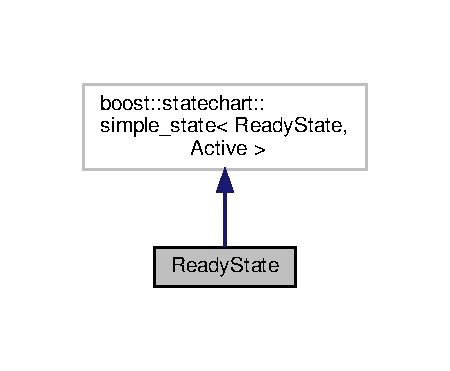
\includegraphics[width=216pt]{structReadyState__inherit__graph}
\end{center}
\end{figure}


Collaboration diagram for Ready\+State\+:
\nopagebreak
\begin{figure}[H]
\begin{center}
\leavevmode
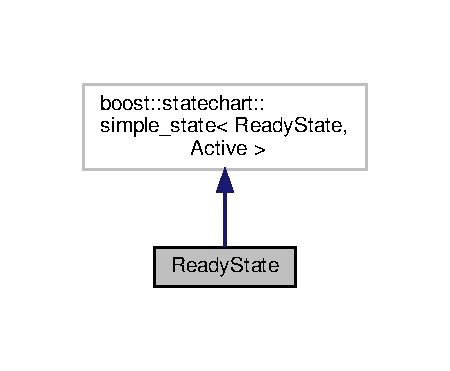
\includegraphics[width=216pt]{structReadyState__coll__graph}
\end{center}
\end{figure}
\subsection*{Public Types}
\begin{DoxyCompactItemize}
\item 
\mbox{\Hypertarget{structReadyState_a050290b91f18ade78ce2771ce5a6f403}\label{structReadyState_a050290b91f18ade78ce2771ce5a6f403}} 
typedef sc\+::custom\+\_\+reaction$<$ \hyperlink{structEvStart}{Ev\+Start} $>$ {\bfseries reactions}
\end{DoxyCompactItemize}
\subsection*{Public Member Functions}
\begin{DoxyCompactItemize}
\item 
\mbox{\Hypertarget{structReadyState_ab1c600b92f8955dc92cdda4472589e2c}\label{structReadyState_ab1c600b92f8955dc92cdda4472589e2c}} 
sc\+::result {\bfseries react} (const \hyperlink{structEvStart}{Ev\+Start} \&)
\end{DoxyCompactItemize}


The documentation for this struct was generated from the following file\+:\begin{DoxyCompactItemize}
\item 
/home/samuel/\+Desktop/toolcog\+\_\+ws/montecarlo/include/tool\+\_\+expt/\hyperlink{manipulate_8h}{manipulate.\+h}\end{DoxyCompactItemize}

\hypertarget{classRecorder}{}\section{Recorder Class Reference}
\label{classRecorder}\index{Recorder@{Recorder}}


class to export data into csv file  




{\ttfamily \#include $<$recorder.\+h$>$}



Collaboration diagram for Recorder\+:
\nopagebreak
\begin{figure}[H]
\begin{center}
\leavevmode
\includegraphics[width=144pt]{classRecorder__coll__graph}
\end{center}
\end{figure}
\subsection*{Public Member Functions}
\begin{DoxyCompactItemize}
\item 
\mbox{\Hypertarget{classRecorder_af0b4f40e7c67f16b0ffff13712149d78}\label{classRecorder_af0b4f40e7c67f16b0ffff13712149d78}} 
\hyperlink{classRecorder_af0b4f40e7c67f16b0ffff13712149d78}{Recorder} ()
\begin{DoxyCompactList}\small\item\em Construct a new \hyperlink{classRecorder}{Recorder} object. \end{DoxyCompactList}\item 
\mbox{\Hypertarget{classRecorder_a6b3c569577fcdc298d8d4a6a2b96e9a9}\label{classRecorder_a6b3c569577fcdc298d8d4a6a2b96e9a9}} 
virtual \hyperlink{classRecorder_a6b3c569577fcdc298d8d4a6a2b96e9a9}{$\sim$\+Recorder} ()
\begin{DoxyCompactList}\small\item\em Destroy the \hyperlink{classRecorder}{Recorder} object. \end{DoxyCompactList}\item 
void \hyperlink{classRecorder_af6314348fd2c47bd074feb6506b6464d}{save\+Data} (\hyperlink{structdataset}{dataset} d)
\begin{DoxyCompactList}\small\item\em save the data into the records \end{DoxyCompactList}\item 
\mbox{\Hypertarget{classRecorder_a635023e6472fcf2422b4d814936cf771}\label{classRecorder_a635023e6472fcf2422b4d814936cf771}} 
void \hyperlink{classRecorder_a635023e6472fcf2422b4d814936cf771}{save2\+File} ()
\begin{DoxyCompactList}\small\item\em export out to csv file \end{DoxyCompactList}\item 
\mbox{\Hypertarget{classRecorder_a79eefa7ff1ed1f6da3cb1e094d675776}\label{classRecorder_a79eefa7ff1ed1f6da3cb1e094d675776}} 
void \hyperlink{classRecorder_a79eefa7ff1ed1f6da3cb1e094d675776}{clear\+Records} ()
\begin{DoxyCompactList}\small\item\em clear all the records and free up memory \end{DoxyCompactList}\item 
void \hyperlink{classRecorder_a77bb320101cee41ef8c6e3c24829c0a9}{set\+Name} (string ss)
\begin{DoxyCompactList}\small\item\em Set the Name of object. \end{DoxyCompactList}\item 
\mbox{\Hypertarget{classRecorder_ade21528ae33a118fa8ef0a2d1481585f}\label{classRecorder_ade21528ae33a118fa8ef0a2d1481585f}} 
void \hyperlink{classRecorder_ade21528ae33a118fa8ef0a2d1481585f}{show\+Address} ()
\begin{DoxyCompactList}\small\item\em show current pointer address \end{DoxyCompactList}\end{DoxyCompactItemize}
\subsection*{Private Attributes}
\begin{DoxyCompactItemize}
\item 
\mbox{\Hypertarget{classRecorder_a9e7bc99c5b525b9ba90b213b9ceb8b0a}\label{classRecorder_a9e7bc99c5b525b9ba90b213b9ceb8b0a}} 
int {\bfseries fileidx}
\item 
\mbox{\Hypertarget{classRecorder_aa462a9878994011343830c7addf84127}\label{classRecorder_aa462a9878994011343830c7addf84127}} 
int {\bfseries size}
\item 
\mbox{\Hypertarget{classRecorder_a58cefe30b461b4c1ca3791bef272e388}\label{classRecorder_a58cefe30b461b4c1ca3791bef272e388}} 
int {\bfseries idx}
\item 
\mbox{\Hypertarget{classRecorder_a762c30c53f299264670e969b8fe0004d}\label{classRecorder_a762c30c53f299264670e969b8fe0004d}} 
string {\bfseries name}
\item 
\mbox{\Hypertarget{classRecorder_acf45c430df53a77b90b6de1715116770}\label{classRecorder_acf45c430df53a77b90b6de1715116770}} 
struct \hyperlink{structdataset}{dataset} $\ast$ {\bfseries records}
\end{DoxyCompactItemize}


\subsection{Detailed Description}
class to export data into csv file 

\subsection{Member Function Documentation}
\mbox{\Hypertarget{classRecorder_af6314348fd2c47bd074feb6506b6464d}\label{classRecorder_af6314348fd2c47bd074feb6506b6464d}} 
\index{Recorder@{Recorder}!save\+Data@{save\+Data}}
\index{save\+Data@{save\+Data}!Recorder@{Recorder}}
\subsubsection{\texorpdfstring{save\+Data()}{saveData()}}
{\footnotesize\ttfamily void Recorder\+::save\+Data (\begin{DoxyParamCaption}\item[{\hyperlink{structdataset}{dataset}}]{d }\end{DoxyParamCaption})}



save the data into the records 


\begin{DoxyParams}{Parameters}
{\em d} & data to save \\
\hline
\end{DoxyParams}
\mbox{\Hypertarget{classRecorder_a77bb320101cee41ef8c6e3c24829c0a9}\label{classRecorder_a77bb320101cee41ef8c6e3c24829c0a9}} 
\index{Recorder@{Recorder}!set\+Name@{set\+Name}}
\index{set\+Name@{set\+Name}!Recorder@{Recorder}}
\subsubsection{\texorpdfstring{set\+Name()}{setName()}}
{\footnotesize\ttfamily void Recorder\+::set\+Name (\begin{DoxyParamCaption}\item[{string}]{ss }\end{DoxyParamCaption})\hspace{0.3cm}{\ttfamily [inline]}}



Set the Name of object. 


\begin{DoxyParams}{Parameters}
{\em ss} & name \\
\hline
\end{DoxyParams}


The documentation for this class was generated from the following files\+:\begin{DoxyCompactItemize}
\item 
/home/samuel/\+Desktop/toolcog\+\_\+ws/montecarlo/include/tool\+\_\+expt/\hyperlink{recorder_8h}{recorder.\+h}\item 
/home/samuel/\+Desktop/toolcog\+\_\+ws/montecarlo/src/recorder.\+cpp\end{DoxyCompactItemize}

\hypertarget{structShape}{}\section{Shape Struct Reference}
\label{structShape}\index{Shape@{Shape}}


shape for \hyperlink{classGJK}{G\+JK} object Contains verticles of object, eg. A C\+U\+BE have 8 vertices Using Eigen Vector3d format for 3 values coordinates (x,y,z) in type double.  




{\ttfamily \#include $<$gjk.\+h$>$}

\subsection*{Public Attributes}
\begin{DoxyCompactItemize}
\item 
\mbox{\Hypertarget{structShape_acef16f7c783ae0a1be162d3b3ab2fa8c}\label{structShape_acef16f7c783ae0a1be162d3b3ab2fa8c}} 
vector$<$ Vector3d $>$ {\bfseries vertices}
\end{DoxyCompactItemize}


\subsection{Detailed Description}
shape for \hyperlink{classGJK}{G\+JK} object Contains verticles of object, eg. A C\+U\+BE have 8 vertices Using Eigen Vector3d format for 3 values coordinates (x,y,z) in type double. 

The documentation for this struct was generated from the following file\+:\begin{DoxyCompactItemize}
\item 
/home/samuel/\+Desktop/toolcog\+\_\+ws/montecarlo/include/tool\+\_\+expt/\hyperlink{gjk_8h}{gjk.\+h}\end{DoxyCompactItemize}

\hypertarget{structStartup}{}\section{Startup Struct Reference}
\label{structStartup}\index{Startup@{Startup}}


structure for \hyperlink{structStartup}{Startup} state -\/$>$ transit to \hyperlink{structActive}{Active} state upon startup  




{\ttfamily \#include $<$machine.\+h$>$}



Inheritance diagram for Startup\+:
\nopagebreak
\begin{figure}[H]
\begin{center}
\leavevmode
\includegraphics[width=202pt]{structStartup__inherit__graph}
\end{center}
\end{figure}


Collaboration diagram for Startup\+:
\nopagebreak
\begin{figure}[H]
\begin{center}
\leavevmode
\includegraphics[width=202pt]{structStartup__coll__graph}
\end{center}
\end{figure}
\subsection*{Public Types}
\begin{DoxyCompactItemize}
\item 
\mbox{\Hypertarget{structStartup_adb819fed6342f9b211ffc4111ff70080}\label{structStartup_adb819fed6342f9b211ffc4111ff70080}} 
typedef sc\+::custom\+\_\+reaction$<$ \hyperlink{structEvStart}{Ev\+Start} $>$ {\bfseries reactions}
\end{DoxyCompactItemize}
\subsection*{Public Member Functions}
\begin{DoxyCompactItemize}
\item 
\mbox{\Hypertarget{structStartup_a5c2eb9104acf334635199f460487d378}\label{structStartup_a5c2eb9104acf334635199f460487d378}} 
{\bfseries Startup} (my\+\_\+context ctx)
\item 
\mbox{\Hypertarget{structStartup_a5e1f550cefd2f461e8ed83a5c50591c1}\label{structStartup_a5e1f550cefd2f461e8ed83a5c50591c1}} 
sc\+::result {\bfseries react} (const \hyperlink{structEvStart}{Ev\+Start} \&)
\end{DoxyCompactItemize}


\subsection{Detailed Description}
structure for \hyperlink{structStartup}{Startup} state -\/$>$ transit to \hyperlink{structActive}{Active} state upon startup 

The documentation for this struct was generated from the following files\+:\begin{DoxyCompactItemize}
\item 
/home/samuel/\+Desktop/toolcog\+\_\+ws/montecarlo/include/tool\+\_\+expt/\hyperlink{machine_8h}{machine.\+h}\item 
/home/samuel/\+Desktop/toolcog\+\_\+ws/montecarlo/src/machine.\+cpp\item 
/home/samuel/\+Desktop/toolcog\+\_\+ws/montecarlo/src/machine\+\_\+sim.\+cpp\end{DoxyCompactItemize}

\hypertarget{classTool__Expt}{}\section{Tool\+\_\+\+Expt Class Reference}
\label{classTool__Expt}\index{Tool\+\_\+\+Expt@{Tool\+\_\+\+Expt}}


Tool experiment class object save all the data and variables used for the tool experiment computes and create task, Handles and directs the M\+C\+TS experiment.  




{\ttfamily \#include $<$tool\+\_\+expt.\+h$>$}



Inheritance diagram for Tool\+\_\+\+Expt\+:
\nopagebreak
\begin{figure}[H]
\begin{center}
\leavevmode
\includegraphics[width=151pt]{classTool__Expt__inherit__graph}
\end{center}
\end{figure}


Collaboration diagram for Tool\+\_\+\+Expt\+:
\nopagebreak
\begin{figure}[H]
\begin{center}
\leavevmode
\includegraphics[width=350pt]{classTool__Expt__coll__graph}
\end{center}
\end{figure}
\subsection*{Public Member Functions}
\begin{DoxyCompactItemize}
\item 
\mbox{\Hypertarget{classTool__Expt_a6f244696f380875f00de3bfa4fd07403}\label{classTool__Expt_a6f244696f380875f00de3bfa4fd07403}} 
\hyperlink{classTool__Expt_a6f244696f380875f00de3bfa4fd07403}{Tool\+\_\+\+Expt} ()
\begin{DoxyCompactList}\small\item\em Construct a new \hyperlink{classTool__Expt}{Tool\+\_\+\+Expt} object. \end{DoxyCompactList}\item 
\mbox{\Hypertarget{classTool__Expt_af70ca9eca501d73dc41e548b33463aa9}\label{classTool__Expt_af70ca9eca501d73dc41e548b33463aa9}} 
\hyperlink{classTool__Expt_af70ca9eca501d73dc41e548b33463aa9}{$\sim$\+Tool\+\_\+\+Expt} ()
\begin{DoxyCompactList}\small\item\em Destroy the \hyperlink{classTool__Expt}{Tool\+\_\+\+Expt} object. \end{DoxyCompactList}\item 
void \hyperlink{classTool__Expt_ac7fc861acae5fc088acda4034cd1ef7b}{init} (\hyperlink{classCreate__Tool}{Create\+\_\+\+Tool} $\ast$\hyperlink{classTool__Expt_ae15dbe96d503e8c03cb86d9f8e58937c}{create\+\_\+tool}, \hyperlink{classMCT__Search}{M\+C\+T\+\_\+\+Search} $\ast$mct\+\_\+search, geometry\+\_\+msgs\+::\+Pose obj\+\_\+pose, geometry\+\_\+msgs\+::\+Pose tar\+\_\+pose)
\begin{DoxyCompactList}\small\item\em tool experiment initialization \end{DoxyCompactList}\item 
void \hyperlink{classTool__Expt_a9bd0a2a625f485202d48636fcc920f04}{init\+\_\+params} (double obj\+\_\+dia, int num\+\_\+via\+\_\+pts, int num\+\_\+intra\+\_\+pts, int max\+\_\+iteration)
\begin{DoxyCompactList}\small\item\em initialise other parameters used in the experiment \end{DoxyCompactList}\item 
void \hyperlink{classTool__Expt_a37cf2a6c1c96828464c9db13ac6a8577}{init\+\_\+vision} (\hyperlink{structvision__each}{vision\+\_\+each} v\+\_\+data, bool percept=true)
\begin{DoxyCompactList}\small\item\em initialise vision data obtain from perception module \end{DoxyCompactList}\item 
\mbox{\Hypertarget{classTool__Expt_a9a0a2083192ef14bac6290b6635a28ed}\label{classTool__Expt_a9a0a2083192ef14bac6290b6635a28ed}} 
void \hyperlink{classTool__Expt_a9a0a2083192ef14bac6290b6635a28ed}{main} ()
\begin{DoxyCompactList}\small\item\em standalone main function to test experiment outside of state machine \end{DoxyCompactList}\item 
Affine3d \hyperlink{classTool__Expt_a6d0d9c6287de98e81b26dff9e0e56863}{create\+\_\+affine} (double roll, double pitch, double yaw, double x, double y, double z)
\begin{DoxyCompactList}\small\item\em Create an eigen affine. \end{DoxyCompactList}\item 
Affine3d \hyperlink{classTool__Expt_a759fb0ce1b71d3153378e7897bef6f72}{create\+\_\+affine} (double roll, double pitch, double yaw, Vector3d xyz)
\begin{DoxyCompactList}\small\item\em Create a eigen affine. \end{DoxyCompactList}\item 
\mbox{\Hypertarget{classTool__Expt_ad17747000a73814a34841eecda0ccc6a}\label{classTool__Expt_ad17747000a73814a34841eecda0ccc6a}} 
void \hyperlink{classTool__Expt_ad17747000a73814a34841eecda0ccc6a}{create\+\_\+task} ()
\begin{DoxyCompactList}\small\item\em Create the task. set up object, target and object\+\_\+to\+\_\+target vector and poses. \end{DoxyCompactList}\item 
\mbox{\Hypertarget{classTool__Expt_ae15dbe96d503e8c03cb86d9f8e58937c}\label{classTool__Expt_ae15dbe96d503e8c03cb86d9f8e58937c}} 
void \hyperlink{classTool__Expt_ae15dbe96d503e8c03cb86d9f8e58937c}{create\+\_\+tool} ()
\begin{DoxyCompactList}\small\item\em Create a tool. compute and set up tool vector and poses. \end{DoxyCompactList}\item 
\mbox{\Hypertarget{classTool__Expt_ae4e9248dd93aa40ad2dd8ae11cf694b7}\label{classTool__Expt_ae4e9248dd93aa40ad2dd8ae11cf694b7}} 
void \hyperlink{classTool__Expt_ae4e9248dd93aa40ad2dd8ae11cf694b7}{create\+\_\+object} ()
\begin{DoxyCompactList}\small\item\em Create a object. generate the object vertices and get ready for gjk collision check. set up object bounding box. \end{DoxyCompactList}\item 
bool \hyperlink{classTool__Expt_a35d5f7c664b44e813c3e1777b723d651}{collision\+\_\+check} ()
\begin{DoxyCompactList}\small\item\em perform \hyperlink{classGJK}{G\+JK} collision check \end{DoxyCompactList}\item 
\mbox{\Hypertarget{classTool__Expt_a1909c4d9fad319e93cc7b92159e1b05f}\label{classTool__Expt_a1909c4d9fad319e93cc7b92159e1b05f}} 
void \hyperlink{classTool__Expt_a1909c4d9fad319e93cc7b92159e1b05f}{create\+\_\+path} ()
\begin{DoxyCompactList}\small\item\em Create all the via points between target and object. \end{DoxyCompactList}\item 
\mbox{\Hypertarget{classTool__Expt_a349b001e0a91bb223e6cd91622818b91}\label{classTool__Expt_a349b001e0a91bb223e6cd91622818b91}} 
void \hyperlink{classTool__Expt_a349b001e0a91bb223e6cd91622818b91}{functionality} ()
\begin{DoxyCompactList}\small\item\em create the task function matrix and object\+\_\+to\+\_\+functionality tf matrix. \end{DoxyCompactList}\item 
\mbox{\Hypertarget{classTool__Expt_a317cc269d335366dec7d88fdf27e5f68}\label{classTool__Expt_a317cc269d335366dec7d88fdf27e5f68}} 
void \hyperlink{classTool__Expt_a317cc269d335366dec7d88fdf27e5f68}{search} ()
\begin{DoxyCompactList}\small\item\em send all the data over to search class obj and perform M\+C\+TS tree search \end{DoxyCompactList}\item 
\mbox{\Hypertarget{classTool__Expt_a53445178c772777722446614d5f3a966}\label{classTool__Expt_a53445178c772777722446614d5f3a966}} 
void \hyperlink{classTool__Expt_a53445178c772777722446614d5f3a966}{create\+\_\+percept\+\_\+tool} ()
\begin{DoxyCompactList}\small\item\em Create a percept tool object. This function creates tool object from perception data. compute and set up tool vector and poses. \end{DoxyCompactList}\item 
vector$<$ Affine3d $>$ \hyperlink{classTool__Expt_a0cace0822f22745b9aa5b7abaa2cec2b}{get\+Result} ()
\begin{DoxyCompactList}\small\item\em Get the Resulting best Path to follow to pull/push object. \end{DoxyCompactList}\item 
Affine3d \hyperlink{classTool__Expt_ad6ca5e51647eee6b267bf51bed8de6a7}{get\+Grab} ()
\begin{DoxyCompactList}\small\item\em Get the Resulting best Grab pose. \end{DoxyCompactList}\item 
double \hyperlink{classTool__Expt_ae29bee730a8bbd7b0a183af404bb366f}{get\+Atk\+Angle} ()
\begin{DoxyCompactList}\small\item\em Get the Resulting best attach angle of the tool to object. \end{DoxyCompactList}\item 
double \hyperlink{classTool__Expt_a1fb8b0a8c2fe25b5e909dcde87b34dd3}{get\+Score} ()
\begin{DoxyCompactList}\small\item\em Get the Score of the best solution. \end{DoxyCompactList}\end{DoxyCompactItemize}
\subsection*{Public Attributes}
\begin{DoxyCompactItemize}
\item 
\mbox{\Hypertarget{classTool__Expt_a1dda864e4413125a1eb1e335171c9487}\label{classTool__Expt_a1dda864e4413125a1eb1e335171c9487}} 
bool {\bfseries percept\+Flag}
\item 
\mbox{\Hypertarget{classTool__Expt_ab9b881e79fbe7c802c1fee961a67edb7}\label{classTool__Expt_ab9b881e79fbe7c802c1fee961a67edb7}} 
bool {\bfseries param\+Flag}
\item 
\mbox{\Hypertarget{classTool__Expt_a4e85b2c1eeb6df93475a1b91d2814cf0}\label{classTool__Expt_a4e85b2c1eeb6df93475a1b91d2814cf0}} 
double {\bfseries m\+\_\+obj\+\_\+dia}
\item 
\mbox{\Hypertarget{classTool__Expt_a39bd18941664411fbdc58dfdc5e08247}\label{classTool__Expt_a39bd18941664411fbdc58dfdc5e08247}} 
int {\bfseries N\+\_\+via\+\_\+pts}
\item 
\mbox{\Hypertarget{classTool__Expt_a8ca80d494109ba43354e8ba6b4860c24}\label{classTool__Expt_a8ca80d494109ba43354e8ba6b4860c24}} 
int {\bfseries N\+\_\+intrapath\+\_\+pts}
\item 
\mbox{\Hypertarget{classTool__Expt_a76afe1d39cf6c333f874a994df98ad71}\label{classTool__Expt_a76afe1d39cf6c333f874a994df98ad71}} 
int {\bfseries N\+\_\+path\+\_\+pts}
\item 
\mbox{\Hypertarget{classTool__Expt_a1168be1098d4588f88898980d05d20f3}\label{classTool__Expt_a1168be1098d4588f88898980d05d20f3}} 
geometry\+\_\+msgs\+::\+Pose {\bfseries m\+\_\+obj\+\_\+pose}
\item 
\mbox{\Hypertarget{classTool__Expt_a6ae2cc487858888b1b618cc663945790}\label{classTool__Expt_a6ae2cc487858888b1b618cc663945790}} 
geometry\+\_\+msgs\+::\+Pose {\bfseries m\+\_\+tar\+\_\+pose}
\item 
\mbox{\Hypertarget{classTool__Expt_a4b0b77f19ef13848df7d207df0eb4e17}\label{classTool__Expt_a4b0b77f19ef13848df7d207df0eb4e17}} 
Affine3d {\bfseries obj\+\_\+affine}
\item 
\mbox{\Hypertarget{classTool__Expt_a19a6a35069a280a506705386e4ccb808}\label{classTool__Expt_a19a6a35069a280a506705386e4ccb808}} 
Affine3d {\bfseries tar\+\_\+affine}
\item 
\mbox{\Hypertarget{classTool__Expt_a06d1e46d87e5f9bad285be4d3c8564cf}\label{classTool__Expt_a06d1e46d87e5f9bad285be4d3c8564cf}} 
Vector3d {\bfseries obj\+\_\+pos}
\item 
\mbox{\Hypertarget{classTool__Expt_ac661b0f3c0cde863b049080acb650cac}\label{classTool__Expt_ac661b0f3c0cde863b049080acb650cac}} 
Vector3d {\bfseries tar\+\_\+pos}
\item 
\mbox{\Hypertarget{classTool__Expt_a2b9adb9f74761aa9be40e89c67389559}\label{classTool__Expt_a2b9adb9f74761aa9be40e89c67389559}} 
Vector3d {\bfseries tool\+\_\+pos}
\item 
\mbox{\Hypertarget{classTool__Expt_af98857e25cd839ab9887746793655d47}\label{classTool__Expt_af98857e25cd839ab9887746793655d47}} 
Vector3d {\bfseries via\+\_\+pt}
\item 
\mbox{\Hypertarget{classTool__Expt_a5deefee78883611c3317d92b7cfe63ea}\label{classTool__Expt_a5deefee78883611c3317d92b7cfe63ea}} 
vector$<$ Affine3d $>$ {\bfseries T\+\_\+world\+\_\+obj}
\item 
\mbox{\Hypertarget{classTool__Expt_a1e489a80d56cae13e9bde5c7066d6dbc}\label{classTool__Expt_a1e489a80d56cae13e9bde5c7066d6dbc}} 
Vector3d {\bfseries obj\+\_\+task}
\item 
\mbox{\Hypertarget{classTool__Expt_a634418684086eb5bac9009cfc1da11d7}\label{classTool__Expt_a634418684086eb5bac9009cfc1da11d7}} 
double {\bfseries angle\+\_\+obj\+\_\+task}
\item 
\mbox{\Hypertarget{classTool__Expt_aaf040fdacac27ee03360d04dab647077}\label{classTool__Expt_aaf040fdacac27ee03360d04dab647077}} 
Affine3d {\bfseries T\+\_\+obj\+\_\+task}
\item 
\mbox{\Hypertarget{classTool__Expt_a71ce08c1a0a9f5dd4ed7ee5b9d070d1b}\label{classTool__Expt_a71ce08c1a0a9f5dd4ed7ee5b9d070d1b}} 
vector$<$ Vector3d $>$ {\bfseries path\+\_\+pts}
\item 
\mbox{\Hypertarget{classTool__Expt_a10152fd0b955160cbf82bd464a8dba22}\label{classTool__Expt_a10152fd0b955160cbf82bd464a8dba22}} 
vector$<$ Affine3d $>$ {\bfseries T\+\_\+all\+\_\+path\+\_\+pts}
\item 
\mbox{\Hypertarget{classTool__Expt_a480f0bd09995c739a0df8e13fa8a49c4}\label{classTool__Expt_a480f0bd09995c739a0df8e13fa8a49c4}} 
\hyperlink{classCreate__Tool}{Create\+\_\+\+Tool} $\ast$ {\bfseries m\+\_\+create\+\_\+tool}
\item 
\mbox{\Hypertarget{classTool__Expt_a6e42a261327a333699868cd3b0e8725d}\label{classTool__Expt_a6e42a261327a333699868cd3b0e8725d}} 
\hyperlink{structShape}{Shape} {\bfseries subtool1}
\item 
\mbox{\Hypertarget{classTool__Expt_a6f6bfc3e326723d029e8f14f8a6da403}\label{classTool__Expt_a6f6bfc3e326723d029e8f14f8a6da403}} 
\hyperlink{structShape}{Shape} {\bfseries subtool2}
\item 
\mbox{\Hypertarget{classTool__Expt_a81dcc95335cf6ace27fa04cf28f90997}\label{classTool__Expt_a81dcc95335cf6ace27fa04cf28f90997}} 
\hyperlink{structShape}{Shape} {\bfseries object}
\item 
\mbox{\Hypertarget{classTool__Expt_aa72fab0ca7d9ee6074e62e017e3303d1}\label{classTool__Expt_aa72fab0ca7d9ee6074e62e017e3303d1}} 
\hyperlink{structvision__each}{vision\+\_\+each} {\bfseries vdata}
\item 
\mbox{\Hypertarget{classTool__Expt_adbdfe0bba7f8bca47948dd24a9224cfd}\label{classTool__Expt_adbdfe0bba7f8bca47948dd24a9224cfd}} 
vector$<$ \hyperlink{structShape}{Shape} $>$ {\bfseries tool\+\_\+pieces}
\item 
\mbox{\Hypertarget{classTool__Expt_a145601ee150aea9eb214a691973d4671}\label{classTool__Expt_a145601ee150aea9eb214a691973d4671}} 
\hyperlink{classGJK}{G\+JK} {\bfseries m\+\_\+gjk}
\item 
\mbox{\Hypertarget{classTool__Expt_ae847e688d5ff22aeb80fafda679909f2}\label{classTool__Expt_ae847e688d5ff22aeb80fafda679909f2}} 
int {\bfseries max\+\_\+iter}
\item 
\mbox{\Hypertarget{classTool__Expt_a9a0a21e153e26e58389ac38e96bce0df}\label{classTool__Expt_a9a0a21e153e26e58389ac38e96bce0df}} 
\hyperlink{structFunc__Templ}{Func\+\_\+\+Templ} {\bfseries m\+\_\+func\+\_\+templ}
\item 
\mbox{\Hypertarget{classTool__Expt_a522f578d3e960ef521b38b679be470b4}\label{classTool__Expt_a522f578d3e960ef521b38b679be470b4}} 
double {\bfseries angle\+\_\+task\+\_\+func}
\item 
\mbox{\Hypertarget{classTool__Expt_acdab35698a6af1afa27579a03a6b5f23}\label{classTool__Expt_acdab35698a6af1afa27579a03a6b5f23}} 
Affine3d {\bfseries T\+\_\+task\+\_\+func}
\item 
\mbox{\Hypertarget{classTool__Expt_a42fb484a1a22411803e0f1ea78ef6563}\label{classTool__Expt_a42fb484a1a22411803e0f1ea78ef6563}} 
vector$<$ Affine3d $>$ {\bfseries T\+\_\+obj\+\_\+func}
\item 
\mbox{\Hypertarget{classTool__Expt_a676a178c660520ac75c89094653fe662}\label{classTool__Expt_a676a178c660520ac75c89094653fe662}} 
\hyperlink{classMCT__Search}{M\+C\+T\+\_\+\+Search} $\ast$ {\bfseries m\+\_\+mct\+\_\+search}
\end{DoxyCompactItemize}
\subsection*{Private Attributes}
\begin{DoxyCompactItemize}
\item 
\mbox{\Hypertarget{classTool__Expt_ac6b5619c61756f3f3749649603a8ce87}\label{classTool__Expt_ac6b5619c61756f3f3749649603a8ce87}} 
vector$<$ Affine3d $>$ {\bfseries result}
\item 
\mbox{\Hypertarget{classTool__Expt_a11ce5889eb57760312df22b12964b69e}\label{classTool__Expt_a11ce5889eb57760312df22b12964b69e}} 
Affine3d {\bfseries result\+\_\+grab}
\item 
\mbox{\Hypertarget{classTool__Expt_a0d5edb8882f8313a4e3ac4e00399c671}\label{classTool__Expt_a0d5edb8882f8313a4e3ac4e00399c671}} 
double {\bfseries result\+\_\+atk}
\item 
\mbox{\Hypertarget{classTool__Expt_a1c722dcf3fe2539d6c79f1c0cd364bc1}\label{classTool__Expt_a1c722dcf3fe2539d6c79f1c0cd364bc1}} 
double {\bfseries max\+\_\+score}
\end{DoxyCompactItemize}


\subsection{Detailed Description}
Tool experiment class object save all the data and variables used for the tool experiment computes and create task, Handles and directs the M\+C\+TS experiment. 

\subsection{Member Function Documentation}
\mbox{\Hypertarget{classTool__Expt_a35d5f7c664b44e813c3e1777b723d651}\label{classTool__Expt_a35d5f7c664b44e813c3e1777b723d651}} 
\index{Tool\+\_\+\+Expt@{Tool\+\_\+\+Expt}!collision\+\_\+check@{collision\+\_\+check}}
\index{collision\+\_\+check@{collision\+\_\+check}!Tool\+\_\+\+Expt@{Tool\+\_\+\+Expt}}
\subsubsection{\texorpdfstring{collision\+\_\+check()}{collision\_check()}}
{\footnotesize\ttfamily bool Tool\+\_\+\+Expt\+::collision\+\_\+check (\begin{DoxyParamCaption}{ }\end{DoxyParamCaption})}



perform \hyperlink{classGJK}{G\+JK} collision check 

\begin{DoxyReturn}{Returns}
true collided 

false no collision 
\end{DoxyReturn}
\mbox{\Hypertarget{classTool__Expt_a6d0d9c6287de98e81b26dff9e0e56863}\label{classTool__Expt_a6d0d9c6287de98e81b26dff9e0e56863}} 
\index{Tool\+\_\+\+Expt@{Tool\+\_\+\+Expt}!create\+\_\+affine@{create\+\_\+affine}}
\index{create\+\_\+affine@{create\+\_\+affine}!Tool\+\_\+\+Expt@{Tool\+\_\+\+Expt}}
\subsubsection{\texorpdfstring{create\+\_\+affine()}{create\_affine()}\hspace{0.1cm}{\footnotesize\ttfamily [1/2]}}
{\footnotesize\ttfamily Affine3d Tool\+\_\+\+Expt\+::create\+\_\+affine (\begin{DoxyParamCaption}\item[{double}]{roll,  }\item[{double}]{pitch,  }\item[{double}]{yaw,  }\item[{double}]{x,  }\item[{double}]{y,  }\item[{double}]{z }\end{DoxyParamCaption})}



Create an eigen affine. 


\begin{DoxyParams}{Parameters}
{\em roll} & \\
\hline
{\em pitch} & \\
\hline
{\em yaw} & \\
\hline
{\em x} & \\
\hline
{\em y} & \\
\hline
{\em z} & \\
\hline
\end{DoxyParams}
\begin{DoxyReturn}{Returns}
Affine3d eigen 
\end{DoxyReturn}
\mbox{\Hypertarget{classTool__Expt_a759fb0ce1b71d3153378e7897bef6f72}\label{classTool__Expt_a759fb0ce1b71d3153378e7897bef6f72}} 
\index{Tool\+\_\+\+Expt@{Tool\+\_\+\+Expt}!create\+\_\+affine@{create\+\_\+affine}}
\index{create\+\_\+affine@{create\+\_\+affine}!Tool\+\_\+\+Expt@{Tool\+\_\+\+Expt}}
\subsubsection{\texorpdfstring{create\+\_\+affine()}{create\_affine()}\hspace{0.1cm}{\footnotesize\ttfamily [2/2]}}
{\footnotesize\ttfamily Affine3d Tool\+\_\+\+Expt\+::create\+\_\+affine (\begin{DoxyParamCaption}\item[{double}]{roll,  }\item[{double}]{pitch,  }\item[{double}]{yaw,  }\item[{Vector3d}]{xyz }\end{DoxyParamCaption})}



Create a eigen affine. 


\begin{DoxyParams}{Parameters}
{\em roll} & \\
\hline
{\em pitch} & \\
\hline
{\em yaw} & \\
\hline
{\em xyz} & \\
\hline
\end{DoxyParams}
\begin{DoxyReturn}{Returns}
Affine3d 
\end{DoxyReturn}
\mbox{\Hypertarget{classTool__Expt_ae29bee730a8bbd7b0a183af404bb366f}\label{classTool__Expt_ae29bee730a8bbd7b0a183af404bb366f}} 
\index{Tool\+\_\+\+Expt@{Tool\+\_\+\+Expt}!get\+Atk\+Angle@{get\+Atk\+Angle}}
\index{get\+Atk\+Angle@{get\+Atk\+Angle}!Tool\+\_\+\+Expt@{Tool\+\_\+\+Expt}}
\subsubsection{\texorpdfstring{get\+Atk\+Angle()}{getAtkAngle()}}
{\footnotesize\ttfamily double Tool\+\_\+\+Expt\+::get\+Atk\+Angle (\begin{DoxyParamCaption}{ }\end{DoxyParamCaption})\hspace{0.3cm}{\ttfamily [inline]}}



Get the Resulting best attach angle of the tool to object. 

\begin{DoxyReturn}{Returns}
double angle 
\end{DoxyReturn}
\mbox{\Hypertarget{classTool__Expt_ad6ca5e51647eee6b267bf51bed8de6a7}\label{classTool__Expt_ad6ca5e51647eee6b267bf51bed8de6a7}} 
\index{Tool\+\_\+\+Expt@{Tool\+\_\+\+Expt}!get\+Grab@{get\+Grab}}
\index{get\+Grab@{get\+Grab}!Tool\+\_\+\+Expt@{Tool\+\_\+\+Expt}}
\subsubsection{\texorpdfstring{get\+Grab()}{getGrab()}}
{\footnotesize\ttfamily Affine3d Tool\+\_\+\+Expt\+::get\+Grab (\begin{DoxyParamCaption}{ }\end{DoxyParamCaption})\hspace{0.3cm}{\ttfamily [inline]}}



Get the Resulting best Grab pose. 

\begin{DoxyReturn}{Returns}
Affine3d grab pose 
\end{DoxyReturn}
\mbox{\Hypertarget{classTool__Expt_a0cace0822f22745b9aa5b7abaa2cec2b}\label{classTool__Expt_a0cace0822f22745b9aa5b7abaa2cec2b}} 
\index{Tool\+\_\+\+Expt@{Tool\+\_\+\+Expt}!get\+Result@{get\+Result}}
\index{get\+Result@{get\+Result}!Tool\+\_\+\+Expt@{Tool\+\_\+\+Expt}}
\subsubsection{\texorpdfstring{get\+Result()}{getResult()}}
{\footnotesize\ttfamily vector$<$ Affine3d $>$ Tool\+\_\+\+Expt\+::get\+Result (\begin{DoxyParamCaption}{ }\end{DoxyParamCaption})\hspace{0.3cm}{\ttfamily [inline]}}



Get the Resulting best Path to follow to pull/push object. 

\begin{DoxyReturn}{Returns}
vector$<$ Affine3d $>$ best path 
\end{DoxyReturn}
\mbox{\Hypertarget{classTool__Expt_a1fb8b0a8c2fe25b5e909dcde87b34dd3}\label{classTool__Expt_a1fb8b0a8c2fe25b5e909dcde87b34dd3}} 
\index{Tool\+\_\+\+Expt@{Tool\+\_\+\+Expt}!get\+Score@{get\+Score}}
\index{get\+Score@{get\+Score}!Tool\+\_\+\+Expt@{Tool\+\_\+\+Expt}}
\subsubsection{\texorpdfstring{get\+Score()}{getScore()}}
{\footnotesize\ttfamily double Tool\+\_\+\+Expt\+::get\+Score (\begin{DoxyParamCaption}{ }\end{DoxyParamCaption})\hspace{0.3cm}{\ttfamily [inline]}}



Get the Score of the best solution. 

\begin{DoxyReturn}{Returns}
double score 
\end{DoxyReturn}
\mbox{\Hypertarget{classTool__Expt_ac7fc861acae5fc088acda4034cd1ef7b}\label{classTool__Expt_ac7fc861acae5fc088acda4034cd1ef7b}} 
\index{Tool\+\_\+\+Expt@{Tool\+\_\+\+Expt}!init@{init}}
\index{init@{init}!Tool\+\_\+\+Expt@{Tool\+\_\+\+Expt}}
\subsubsection{\texorpdfstring{init()}{init()}}
{\footnotesize\ttfamily void Tool\+\_\+\+Expt\+::init (\begin{DoxyParamCaption}\item[{\hyperlink{classCreate__Tool}{Create\+\_\+\+Tool} $\ast$}]{create\+\_\+tool,  }\item[{\hyperlink{classMCT__Search}{M\+C\+T\+\_\+\+Search} $\ast$}]{mct\+\_\+search,  }\item[{geometry\+\_\+msgs\+::\+Pose}]{obj\+\_\+pose,  }\item[{geometry\+\_\+msgs\+::\+Pose}]{tar\+\_\+pose }\end{DoxyParamCaption})}



tool experiment initialization 


\begin{DoxyParams}{Parameters}
{\em create\+\_\+tool} & pointer to create\+\_\+tool obj \\
\hline
{\em mct\+\_\+search} & pointer to mct\+\_\+search obj \\
\hline
{\em obj\+\_\+pose} & object pose \\
\hline
{\em tar\+\_\+pose} & target pose \\
\hline
\end{DoxyParams}
\mbox{\Hypertarget{classTool__Expt_a9bd0a2a625f485202d48636fcc920f04}\label{classTool__Expt_a9bd0a2a625f485202d48636fcc920f04}} 
\index{Tool\+\_\+\+Expt@{Tool\+\_\+\+Expt}!init\+\_\+params@{init\+\_\+params}}
\index{init\+\_\+params@{init\+\_\+params}!Tool\+\_\+\+Expt@{Tool\+\_\+\+Expt}}
\subsubsection{\texorpdfstring{init\+\_\+params()}{init\_params()}}
{\footnotesize\ttfamily void Tool\+\_\+\+Expt\+::init\+\_\+params (\begin{DoxyParamCaption}\item[{double}]{obj\+\_\+dia,  }\item[{int}]{num\+\_\+via\+\_\+pts,  }\item[{int}]{num\+\_\+intra\+\_\+pts,  }\item[{int}]{max\+\_\+iteration }\end{DoxyParamCaption})}



initialise other parameters used in the experiment 


\begin{DoxyParams}{Parameters}
{\em obj\+\_\+dia} & object diameter \\
\hline
{\em num\+\_\+via\+\_\+pts} & number of via points to required \\
\hline
{\em num\+\_\+intra\+\_\+pts} & number of intra path points \\
\hline
{\em max\+\_\+iteration} & number of iterations for mcts \\
\hline
\end{DoxyParams}
\mbox{\Hypertarget{classTool__Expt_a37cf2a6c1c96828464c9db13ac6a8577}\label{classTool__Expt_a37cf2a6c1c96828464c9db13ac6a8577}} 
\index{Tool\+\_\+\+Expt@{Tool\+\_\+\+Expt}!init\+\_\+vision@{init\+\_\+vision}}
\index{init\+\_\+vision@{init\+\_\+vision}!Tool\+\_\+\+Expt@{Tool\+\_\+\+Expt}}
\subsubsection{\texorpdfstring{init\+\_\+vision()}{init\_vision()}}
{\footnotesize\ttfamily void Tool\+\_\+\+Expt\+::init\+\_\+vision (\begin{DoxyParamCaption}\item[{\hyperlink{structvision__each}{vision\+\_\+each}}]{v\+\_\+data,  }\item[{bool}]{percept = {\ttfamily true} }\end{DoxyParamCaption})}



initialise vision data obtain from perception module 


\begin{DoxyParams}{Parameters}
{\em v\+\_\+data} & vision data used for this experiment \\
\hline
{\em percept} & is data obtained from perception module? \\
\hline
\end{DoxyParams}


The documentation for this class was generated from the following files\+:\begin{DoxyCompactItemize}
\item 
/home/samuel/\+Desktop/toolcog\+\_\+ws/montecarlo/include/tool\+\_\+expt/\hyperlink{tool__expt_8h}{tool\+\_\+expt.\+h}\item 
/home/samuel/\+Desktop/toolcog\+\_\+ws/montecarlo/src/tool\+\_\+expt.\+cpp\end{DoxyCompactItemize}

\hypertarget{classTool__Expt__2}{}\section{Tool\+\_\+\+Expt\+\_\+2 Class Reference}
\label{classTool__Expt__2}\index{Tool\+\_\+\+Expt\+\_\+2@{Tool\+\_\+\+Expt\+\_\+2}}


Tool experiment class object save all the data and variables used for the tool experiment computes and create task, Handles and directs the M\+C\+TS experiment version 2.\+0, using the recursive search function + check for obstacles.  




{\ttfamily \#include $<$tool\+\_\+expt2.\+h$>$}



Inheritance diagram for Tool\+\_\+\+Expt\+\_\+2\+:
\nopagebreak
\begin{figure}[H]
\begin{center}
\leavevmode
\includegraphics[width=151pt]{classTool__Expt__2__inherit__graph}
\end{center}
\end{figure}


Collaboration diagram for Tool\+\_\+\+Expt\+\_\+2\+:
\nopagebreak
\begin{figure}[H]
\begin{center}
\leavevmode
\includegraphics[width=350pt]{classTool__Expt__2__coll__graph}
\end{center}
\end{figure}
\subsection*{Public Member Functions}
\begin{DoxyCompactItemize}
\item 
\mbox{\Hypertarget{classTool__Expt__2_a64e26303f2c9a3ee781be8b64e6263cf}\label{classTool__Expt__2_a64e26303f2c9a3ee781be8b64e6263cf}} 
\hyperlink{classTool__Expt__2_a64e26303f2c9a3ee781be8b64e6263cf}{Tool\+\_\+\+Expt\+\_\+2} ()
\begin{DoxyCompactList}\small\item\em Construct a new \hyperlink{classTool__Expt__2}{Tool\+\_\+\+Expt\+\_\+2} object. \end{DoxyCompactList}\item 
\mbox{\Hypertarget{classTool__Expt__2_a8c3e036e424c835e8df639457fe1b63e}\label{classTool__Expt__2_a8c3e036e424c835e8df639457fe1b63e}} 
\hyperlink{classTool__Expt__2_a8c3e036e424c835e8df639457fe1b63e}{$\sim$\+Tool\+\_\+\+Expt\+\_\+2} ()
\begin{DoxyCompactList}\small\item\em Destroy the \hyperlink{classTool__Expt__2}{Tool\+\_\+\+Expt\+\_\+2} object. \end{DoxyCompactList}\item 
void \hyperlink{classTool__Expt__2_a13eb50ab5238d8280ab013faa16df365}{init} (\hyperlink{classCreate__Tool}{Create\+\_\+\+Tool} $\ast$\hyperlink{classTool__Expt_ae15dbe96d503e8c03cb86d9f8e58937c}{create\+\_\+tool}, \hyperlink{classMCT__Search2}{M\+C\+T\+\_\+\+Search2} $\ast$mct\+\_\+search2, geometry\+\_\+msgs\+::\+Pose obj\+\_\+pose, geometry\+\_\+msgs\+::\+Pose tar\+\_\+pose)
\begin{DoxyCompactList}\small\item\em tool experiment initialization \end{DoxyCompactList}\item 
void \hyperlink{classTool__Expt__2_ab6fdd7dd20018e9d90b12e6f14ea3911}{init\+\_\+params} (double obj\+\_\+dia, double obst\+\_\+dia, double num\+\_\+candidates, geometry\+\_\+msgs\+::\+Pose obst\+\_\+pose, int max\+\_\+iteration)
\begin{DoxyCompactList}\small\item\em initialise other parameters used in the experiment \end{DoxyCompactList}\item 
\mbox{\Hypertarget{classTool__Expt__2_a3aa54fd0444cf6c21987c3e77470e110}\label{classTool__Expt__2_a3aa54fd0444cf6c21987c3e77470e110}} 
void \hyperlink{classTool__Expt__2_a3aa54fd0444cf6c21987c3e77470e110}{main} ()
\begin{DoxyCompactList}\small\item\em standalone main function to test experiment outside state machine \end{DoxyCompactList}\item 
\mbox{\Hypertarget{classTool__Expt__2_a22b3644a88a85a6864672f3dafbb4d25}\label{classTool__Expt__2_a22b3644a88a85a6864672f3dafbb4d25}} 
void \hyperlink{classTool__Expt__2_a22b3644a88a85a6864672f3dafbb4d25}{create\+\_\+obstacle} ()
\begin{DoxyCompactList}\small\item\em Create a obstacle object and draw the bounding box for thee obstacle. \end{DoxyCompactList}\item 
\mbox{\Hypertarget{classTool__Expt__2_a71b3d3747f2e06a63799812c434df6a2}\label{classTool__Expt__2_a71b3d3747f2e06a63799812c434df6a2}} 
void \hyperlink{classTool__Expt__2_a71b3d3747f2e06a63799812c434df6a2}{obstruction\+\_\+check} ()
\begin{DoxyCompactList}\small\item\em check if object to target is being blocked by obstacle \end{DoxyCompactList}\item 
\mbox{\Hypertarget{classTool__Expt__2_a98d260a9657ddce4ef0811649851d886}\label{classTool__Expt__2_a98d260a9657ddce4ef0811649851d886}} 
void \hyperlink{classTool__Expt__2_a98d260a9657ddce4ef0811649851d886}{create\+\_\+path} ()
\begin{DoxyCompactList}\small\item\em Create all the via points between target and object if obstructed by obstacle, use candidate via points to avoid. \end{DoxyCompactList}\item 
\mbox{\Hypertarget{classTool__Expt__2_a56a331ac5f5fe40e070466b97f746a21}\label{classTool__Expt__2_a56a331ac5f5fe40e070466b97f746a21}} 
void \hyperlink{classTool__Expt__2_a56a331ac5f5fe40e070466b97f746a21}{functionality} ()
\begin{DoxyCompactList}\small\item\em create the task function matrix and object\+\_\+to\+\_\+functionality tf matrix. \end{DoxyCompactList}\item 
\mbox{\Hypertarget{classTool__Expt__2_ac9e4fdba0c08996bc46cd9e74f878383}\label{classTool__Expt__2_ac9e4fdba0c08996bc46cd9e74f878383}} 
void \hyperlink{classTool__Expt__2_ac9e4fdba0c08996bc46cd9e74f878383}{search} ()
\begin{DoxyCompactList}\small\item\em send all the data over to search class obj and perform M\+C\+TS tree search \end{DoxyCompactList}\item 
vector$<$ Affine3d $>$ \hyperlink{classTool__Expt__2_ae984275561905b857cf025239efc0a2c}{get\+Result} ()
\begin{DoxyCompactList}\small\item\em Get the Resulting best Path to follow to pull/push object. \end{DoxyCompactList}\item 
Affine3d \hyperlink{classTool__Expt__2_a5952622f42e4bc903c46180eb63142ee}{get\+Grab} ()
\begin{DoxyCompactList}\small\item\em Get the Resulting best Grab pose. \end{DoxyCompactList}\item 
double \hyperlink{classTool__Expt__2_a30ce22966534df289b16a55cd8a1636f}{get\+Atk\+Angle} ()
\begin{DoxyCompactList}\small\item\em Get the Resulting best attach angle of the tool to object. \end{DoxyCompactList}\item 
double \hyperlink{classTool__Expt__2_a914a228608477de677f9045fe6bf3c08}{get\+Score} ()
\begin{DoxyCompactList}\small\item\em Get the Score of the best solution. \end{DoxyCompactList}\item 
Vector3d \hyperlink{classTool__Expt__2_a9247b27356d4972cdb911120cc1920cb}{get\+Via\+Pt} ()
\begin{DoxyCompactList}\small\item\em Get the Via Pt to use from the best solution to avoid obstacle. \end{DoxyCompactList}\item 
bool \hyperlink{classTool__Expt__2_a4f325224bd61c8d68d562a02f84d90c3}{get\+Obstruct} ()
\begin{DoxyCompactList}\small\item\em Get the Obstruction. Check if obstructed. \end{DoxyCompactList}\end{DoxyCompactItemize}
\subsection*{Public Attributes}
\begin{DoxyCompactItemize}
\item 
\mbox{\Hypertarget{classTool__Expt__2_afe0cdde93d9fa08f0cab5f3b9ad43127}\label{classTool__Expt__2_afe0cdde93d9fa08f0cab5f3b9ad43127}} 
int {\bfseries N\+\_\+via\+\_\+candidates}
\item 
\mbox{\Hypertarget{classTool__Expt__2_a69b682644f21f9266c2b8423d44e723c}\label{classTool__Expt__2_a69b682644f21f9266c2b8423d44e723c}} 
bool {\bfseries obstruct\+\_\+flag}
\item 
\mbox{\Hypertarget{classTool__Expt__2_abcb49647ce6c224dfa504269461ce58c}\label{classTool__Expt__2_abcb49647ce6c224dfa504269461ce58c}} 
double {\bfseries m\+\_\+obst\+\_\+dia}
\item 
\mbox{\Hypertarget{classTool__Expt__2_ad30eec8c81aed75a5938d8311330f298}\label{classTool__Expt__2_ad30eec8c81aed75a5938d8311330f298}} 
geometry\+\_\+msgs\+::\+Pose {\bfseries m\+\_\+obst\+\_\+pose}
\item 
\mbox{\Hypertarget{classTool__Expt__2_aa39e482536af894df89c2960ddabb93f}\label{classTool__Expt__2_aa39e482536af894df89c2960ddabb93f}} 
\hyperlink{structShape}{Shape} {\bfseries obstacle}
\item 
\mbox{\Hypertarget{classTool__Expt__2_a0a84e97236e044343b9e4adc6dfacbc7}\label{classTool__Expt__2_a0a84e97236e044343b9e4adc6dfacbc7}} 
Affine3d {\bfseries obst\+\_\+affine}
\item 
\mbox{\Hypertarget{classTool__Expt__2_afb2f932f6f5aa555677deb46531aaab9}\label{classTool__Expt__2_afb2f932f6f5aa555677deb46531aaab9}} 
Vector3d {\bfseries obst\+\_\+pos}
\item 
\mbox{\Hypertarget{classTool__Expt__2_ab1366bd2676ac5ed02d2fb74370d2726}\label{classTool__Expt__2_ab1366bd2676ac5ed02d2fb74370d2726}} 
vector$<$ Vector3d $>$ {\bfseries via\+\_\+pts}
\item 
\mbox{\Hypertarget{classTool__Expt__2_a4e371a2745f78ee64f3c36bc16085cf9}\label{classTool__Expt__2_a4e371a2745f78ee64f3c36bc16085cf9}} 
Vector3d {\bfseries obj\+\_\+via}
\item 
\mbox{\Hypertarget{classTool__Expt__2_afb30ed9a74d6936cedbdb3899e4328cd}\label{classTool__Expt__2_afb30ed9a74d6936cedbdb3899e4328cd}} 
double {\bfseries angle\+\_\+obj\+\_\+via}
\item 
\mbox{\Hypertarget{classTool__Expt__2_a3b620187bb7345a02ffb2e8704961208}\label{classTool__Expt__2_a3b620187bb7345a02ffb2e8704961208}} 
Affine3d {\bfseries T\+\_\+obj\+\_\+via}
\item 
\mbox{\Hypertarget{classTool__Expt__2_af8d43750625b98a106c6606184ce522a}\label{classTool__Expt__2_af8d43750625b98a106c6606184ce522a}} 
Vector3d {\bfseries via\+\_\+tar}
\item 
\mbox{\Hypertarget{classTool__Expt__2_aa39d0a14d97237c421cd049bebc358c4}\label{classTool__Expt__2_aa39d0a14d97237c421cd049bebc358c4}} 
double {\bfseries angle\+\_\+via\+\_\+tar}
\item 
\mbox{\Hypertarget{classTool__Expt__2_a3e286ff433b47843641bd659dee2afb0}\label{classTool__Expt__2_a3e286ff433b47843641bd659dee2afb0}} 
Affine3d {\bfseries T\+\_\+via\+\_\+tar}
\item 
\mbox{\Hypertarget{classTool__Expt__2_a98ffffb3f89e1f64d964b8485ab213f8}\label{classTool__Expt__2_a98ffffb3f89e1f64d964b8485ab213f8}} 
Affine3d {\bfseries T\+\_\+task\+\_\+func\+\_\+wt\+\_\+gap}
\item 
\mbox{\Hypertarget{classTool__Expt__2_a0189882749568e8c1661bf31efbca1cc}\label{classTool__Expt__2_a0189882749568e8c1661bf31efbca1cc}} 
Affine3d {\bfseries T\+\_\+task\+\_\+func\+\_\+wt\+\_\+gap\+\_\+1}
\item 
\mbox{\Hypertarget{classTool__Expt__2_a64e1f0372fa2f43eb1fe1f48131d8904}\label{classTool__Expt__2_a64e1f0372fa2f43eb1fe1f48131d8904}} 
vector$<$ vector$<$ Affine3d $>$ $>$ {\bfseries all\+\_\+\+T\+\_\+world\+\_\+obj\+\_\+bb}
\item 
\mbox{\Hypertarget{classTool__Expt__2_a0d73b60245a5ec480e482e8cd4165e55}\label{classTool__Expt__2_a0d73b60245a5ec480e482e8cd4165e55}} 
vector$<$ vector$<$ Affine3d $>$ $>$ {\bfseries all\+\_\+\+T\+\_\+world\+\_\+obst\+\_\+bb}
\item 
\mbox{\Hypertarget{classTool__Expt__2_aec3e58756302427e7c854a314125d5a2}\label{classTool__Expt__2_aec3e58756302427e7c854a314125d5a2}} 
vector$<$ vector$<$ Affine3d $>$ $>$ {\bfseries all\+\_\+\+T\+\_\+world\+\_\+obj}
\item 
\mbox{\Hypertarget{classTool__Expt__2_ad5e05783f1b2c027108d734135b45a5a}\label{classTool__Expt__2_ad5e05783f1b2c027108d734135b45a5a}} 
vector$<$ vector$<$ Vector3d $>$ $>$ {\bfseries all\+\_\+move\+\_\+vec}
\item 
\mbox{\Hypertarget{classTool__Expt__2_a835dfdb9db3e97dbf80211a04bc8fe5b}\label{classTool__Expt__2_a835dfdb9db3e97dbf80211a04bc8fe5b}} 
vector$<$ vector$<$ Affine3d $>$ $>$ {\bfseries all\+\_\+\+T\+\_\+world\+\_\+func}
\item 
\mbox{\Hypertarget{classTool__Expt__2_a67e3bc6167b42e0cc706ca1f84ecc0cc}\label{classTool__Expt__2_a67e3bc6167b42e0cc706ca1f84ecc0cc}} 
vector$<$ vector$<$ Affine3d $>$ $>$ {\bfseries all\+\_\+\+T\+\_\+obj\+\_\+func}
\item 
\mbox{\Hypertarget{classTool__Expt__2_ad30d37c86882819c277d363575555067}\label{classTool__Expt__2_ad30d37c86882819c277d363575555067}} 
\hyperlink{classMCT__Search2}{M\+C\+T\+\_\+\+Search2} $\ast$ {\bfseries m\+\_\+mct\+\_\+search2}
\end{DoxyCompactItemize}
\subsection*{Private Attributes}
\begin{DoxyCompactItemize}
\item 
\mbox{\Hypertarget{classTool__Expt__2_ab85791e360a8688ac867a69f30263e29}\label{classTool__Expt__2_ab85791e360a8688ac867a69f30263e29}} 
vector$<$ Affine3d $>$ {\bfseries result}
\item 
\mbox{\Hypertarget{classTool__Expt__2_a7c70ddc3710ce4386d14de1626b69ad7}\label{classTool__Expt__2_a7c70ddc3710ce4386d14de1626b69ad7}} 
Vector3d {\bfseries result\+\_\+via\+\_\+pt}
\item 
\mbox{\Hypertarget{classTool__Expt__2_ada099fb22208cf179979d3edda16c669}\label{classTool__Expt__2_ada099fb22208cf179979d3edda16c669}} 
Affine3d {\bfseries result\+\_\+grab}
\item 
\mbox{\Hypertarget{classTool__Expt__2_a1047fce015dcb3a94549eb24955d15f5}\label{classTool__Expt__2_a1047fce015dcb3a94549eb24955d15f5}} 
double {\bfseries result\+\_\+atk}
\item 
\mbox{\Hypertarget{classTool__Expt__2_a5ded0c8a48fea429b07cfafc1dbe4ca8}\label{classTool__Expt__2_a5ded0c8a48fea429b07cfafc1dbe4ca8}} 
double {\bfseries max\+\_\+score}
\end{DoxyCompactItemize}


\subsection{Detailed Description}
Tool experiment class object save all the data and variables used for the tool experiment computes and create task, Handles and directs the M\+C\+TS experiment version 2.\+0, using the recursive search function + check for obstacles. 

\subsection{Member Function Documentation}
\mbox{\Hypertarget{classTool__Expt__2_a30ce22966534df289b16a55cd8a1636f}\label{classTool__Expt__2_a30ce22966534df289b16a55cd8a1636f}} 
\index{Tool\+\_\+\+Expt\+\_\+2@{Tool\+\_\+\+Expt\+\_\+2}!get\+Atk\+Angle@{get\+Atk\+Angle}}
\index{get\+Atk\+Angle@{get\+Atk\+Angle}!Tool\+\_\+\+Expt\+\_\+2@{Tool\+\_\+\+Expt\+\_\+2}}
\subsubsection{\texorpdfstring{get\+Atk\+Angle()}{getAtkAngle()}}
{\footnotesize\ttfamily double Tool\+\_\+\+Expt\+\_\+2\+::get\+Atk\+Angle (\begin{DoxyParamCaption}{ }\end{DoxyParamCaption})\hspace{0.3cm}{\ttfamily [inline]}}



Get the Resulting best attach angle of the tool to object. 

\begin{DoxyReturn}{Returns}
double angle 
\end{DoxyReturn}
\mbox{\Hypertarget{classTool__Expt__2_a5952622f42e4bc903c46180eb63142ee}\label{classTool__Expt__2_a5952622f42e4bc903c46180eb63142ee}} 
\index{Tool\+\_\+\+Expt\+\_\+2@{Tool\+\_\+\+Expt\+\_\+2}!get\+Grab@{get\+Grab}}
\index{get\+Grab@{get\+Grab}!Tool\+\_\+\+Expt\+\_\+2@{Tool\+\_\+\+Expt\+\_\+2}}
\subsubsection{\texorpdfstring{get\+Grab()}{getGrab()}}
{\footnotesize\ttfamily Affine3d Tool\+\_\+\+Expt\+\_\+2\+::get\+Grab (\begin{DoxyParamCaption}{ }\end{DoxyParamCaption})\hspace{0.3cm}{\ttfamily [inline]}}



Get the Resulting best Grab pose. 

\begin{DoxyReturn}{Returns}
Affine3d grab pose 
\end{DoxyReturn}
\mbox{\Hypertarget{classTool__Expt__2_a4f325224bd61c8d68d562a02f84d90c3}\label{classTool__Expt__2_a4f325224bd61c8d68d562a02f84d90c3}} 
\index{Tool\+\_\+\+Expt\+\_\+2@{Tool\+\_\+\+Expt\+\_\+2}!get\+Obstruct@{get\+Obstruct}}
\index{get\+Obstruct@{get\+Obstruct}!Tool\+\_\+\+Expt\+\_\+2@{Tool\+\_\+\+Expt\+\_\+2}}
\subsubsection{\texorpdfstring{get\+Obstruct()}{getObstruct()}}
{\footnotesize\ttfamily bool Tool\+\_\+\+Expt\+\_\+2\+::get\+Obstruct (\begin{DoxyParamCaption}{ }\end{DoxyParamCaption})\hspace{0.3cm}{\ttfamily [inline]}}



Get the Obstruction. Check if obstructed. 

\begin{DoxyReturn}{Returns}
true obstructed 

false not obstructed 
\end{DoxyReturn}
\mbox{\Hypertarget{classTool__Expt__2_ae984275561905b857cf025239efc0a2c}\label{classTool__Expt__2_ae984275561905b857cf025239efc0a2c}} 
\index{Tool\+\_\+\+Expt\+\_\+2@{Tool\+\_\+\+Expt\+\_\+2}!get\+Result@{get\+Result}}
\index{get\+Result@{get\+Result}!Tool\+\_\+\+Expt\+\_\+2@{Tool\+\_\+\+Expt\+\_\+2}}
\subsubsection{\texorpdfstring{get\+Result()}{getResult()}}
{\footnotesize\ttfamily vector$<$ Affine3d $>$ Tool\+\_\+\+Expt\+\_\+2\+::get\+Result (\begin{DoxyParamCaption}{ }\end{DoxyParamCaption})\hspace{0.3cm}{\ttfamily [inline]}}



Get the Resulting best Path to follow to pull/push object. 

\begin{DoxyReturn}{Returns}
vector$<$ Affine3d $>$ best path 
\end{DoxyReturn}
\mbox{\Hypertarget{classTool__Expt__2_a914a228608477de677f9045fe6bf3c08}\label{classTool__Expt__2_a914a228608477de677f9045fe6bf3c08}} 
\index{Tool\+\_\+\+Expt\+\_\+2@{Tool\+\_\+\+Expt\+\_\+2}!get\+Score@{get\+Score}}
\index{get\+Score@{get\+Score}!Tool\+\_\+\+Expt\+\_\+2@{Tool\+\_\+\+Expt\+\_\+2}}
\subsubsection{\texorpdfstring{get\+Score()}{getScore()}}
{\footnotesize\ttfamily double Tool\+\_\+\+Expt\+\_\+2\+::get\+Score (\begin{DoxyParamCaption}{ }\end{DoxyParamCaption})\hspace{0.3cm}{\ttfamily [inline]}}



Get the Score of the best solution. 

\begin{DoxyReturn}{Returns}
double score 
\end{DoxyReturn}
\mbox{\Hypertarget{classTool__Expt__2_a9247b27356d4972cdb911120cc1920cb}\label{classTool__Expt__2_a9247b27356d4972cdb911120cc1920cb}} 
\index{Tool\+\_\+\+Expt\+\_\+2@{Tool\+\_\+\+Expt\+\_\+2}!get\+Via\+Pt@{get\+Via\+Pt}}
\index{get\+Via\+Pt@{get\+Via\+Pt}!Tool\+\_\+\+Expt\+\_\+2@{Tool\+\_\+\+Expt\+\_\+2}}
\subsubsection{\texorpdfstring{get\+Via\+Pt()}{getViaPt()}}
{\footnotesize\ttfamily Vector3d Tool\+\_\+\+Expt\+\_\+2\+::get\+Via\+Pt (\begin{DoxyParamCaption}{ }\end{DoxyParamCaption})\hspace{0.3cm}{\ttfamily [inline]}}



Get the Via Pt to use from the best solution to avoid obstacle. 

\begin{DoxyReturn}{Returns}
Vector3d viapoint translation 
\end{DoxyReturn}
\mbox{\Hypertarget{classTool__Expt__2_a13eb50ab5238d8280ab013faa16df365}\label{classTool__Expt__2_a13eb50ab5238d8280ab013faa16df365}} 
\index{Tool\+\_\+\+Expt\+\_\+2@{Tool\+\_\+\+Expt\+\_\+2}!init@{init}}
\index{init@{init}!Tool\+\_\+\+Expt\+\_\+2@{Tool\+\_\+\+Expt\+\_\+2}}
\subsubsection{\texorpdfstring{init()}{init()}}
{\footnotesize\ttfamily void Tool\+\_\+\+Expt\+\_\+2\+::init (\begin{DoxyParamCaption}\item[{\hyperlink{classCreate__Tool}{Create\+\_\+\+Tool} $\ast$}]{create\+\_\+tool,  }\item[{\hyperlink{classMCT__Search2}{M\+C\+T\+\_\+\+Search2} $\ast$}]{mct\+\_\+search2,  }\item[{geometry\+\_\+msgs\+::\+Pose}]{obj\+\_\+pose,  }\item[{geometry\+\_\+msgs\+::\+Pose}]{tar\+\_\+pose }\end{DoxyParamCaption})}



tool experiment initialization 


\begin{DoxyParams}{Parameters}
{\em create\+\_\+tool} & pointer to create\+\_\+tool obj \\
\hline
{\em mct\+\_\+search} & pointer to mct\+\_\+search obj \\
\hline
{\em obj\+\_\+pose} & object pose \\
\hline
{\em tar\+\_\+pose} & target pose \\
\hline
\end{DoxyParams}
\mbox{\Hypertarget{classTool__Expt__2_ab6fdd7dd20018e9d90b12e6f14ea3911}\label{classTool__Expt__2_ab6fdd7dd20018e9d90b12e6f14ea3911}} 
\index{Tool\+\_\+\+Expt\+\_\+2@{Tool\+\_\+\+Expt\+\_\+2}!init\+\_\+params@{init\+\_\+params}}
\index{init\+\_\+params@{init\+\_\+params}!Tool\+\_\+\+Expt\+\_\+2@{Tool\+\_\+\+Expt\+\_\+2}}
\subsubsection{\texorpdfstring{init\+\_\+params()}{init\_params()}}
{\footnotesize\ttfamily void Tool\+\_\+\+Expt\+\_\+2\+::init\+\_\+params (\begin{DoxyParamCaption}\item[{double}]{obj\+\_\+dia,  }\item[{double}]{obst\+\_\+dia,  }\item[{double}]{num\+\_\+candidates,  }\item[{geometry\+\_\+msgs\+::\+Pose}]{obst\+\_\+pose,  }\item[{int}]{max\+\_\+iteration }\end{DoxyParamCaption})}



initialise other parameters used in the experiment 


\begin{DoxyParams}{Parameters}
{\em obj\+\_\+dia} & object diameter \\
\hline
{\em obst\+\_\+dia} & obstacle diameter \\
\hline
{\em num\+\_\+candidates} & number of via point candidates \\
\hline
{\em obst\+\_\+pose} & obstacle pose \\
\hline
{\em max\+\_\+iteration} & number of iterations for mcts \\
\hline
\end{DoxyParams}


The documentation for this class was generated from the following files\+:\begin{DoxyCompactItemize}
\item 
/home/samuel/\+Desktop/toolcog\+\_\+ws/montecarlo/include/tool\+\_\+expt/\hyperlink{tool__expt2_8h}{tool\+\_\+expt2.\+h}\item 
/home/samuel/\+Desktop/toolcog\+\_\+ws/montecarlo/src/tool\+\_\+expt2.\+cpp\end{DoxyCompactItemize}

\hypertarget{structvision__data}{}\section{vision\+\_\+data Struct Reference}
\label{structvision__data}\index{vision\+\_\+data@{vision\+\_\+data}}


vision data structure for large sets of perceived objects  




{\ttfamily \#include $<$vision\+\_\+data.\+h$>$}

\subsection*{Public Attributes}
\begin{DoxyCompactItemize}
\item 
\mbox{\Hypertarget{structvision__data_a95115b1fce74123383b6c4472745448b}\label{structvision__data_a95115b1fce74123383b6c4472745448b}} 
std\+::vector$<$ float $>$ {\bfseries objhight2table}
\item 
\mbox{\Hypertarget{structvision__data_a1bdd2b23e155c994219099b27a5b486f}\label{structvision__data_a1bdd2b23e155c994219099b27a5b486f}} 
std\+::vector$<$ pcl\+::\+Point\+Cloud$<$ pcl\+::\+Point\+X\+YZ $>$ $>$ {\bfseries hull\+Clusters\+On\+Axis}
\item 
\mbox{\Hypertarget{structvision__data_a2e3628a452aa67ad21669ae1feeadc7d}\label{structvision__data_a2e3628a452aa67ad21669ae1feeadc7d}} 
std\+::vector$<$ Eigen\+::\+Matrix4d $>$ {\bfseries pro2table\+T\+Fs}
\item 
\mbox{\Hypertarget{structvision__data_a71bb8dcc2cfb218345063d77b3208f5f}\label{structvision__data_a71bb8dcc2cfb218345063d77b3208f5f}} 
std\+::vector$<$ std\+::vector$<$ pcl\+::\+Point\+Cloud$<$ pcl\+::\+Point\+X\+YZ $>$ $>$ $>$ {\bfseries tool\+Convex\+Hulls}
\end{DoxyCompactItemize}


\subsection{Detailed Description}
vision data structure for large sets of perceived objects 

The documentation for this struct was generated from the following file\+:\begin{DoxyCompactItemize}
\item 
/home/samuel/\+Desktop/toolcog\+\_\+ws/montecarlo/include/tool\+\_\+expt/\hyperlink{vision__data_8h}{vision\+\_\+data.\+h}\end{DoxyCompactItemize}

\hypertarget{structvision__each}{}\section{vision\+\_\+each Struct Reference}
\label{structvision__each}\index{vision\+\_\+each@{vision\+\_\+each}}


vision data structure for each perceived object  




{\ttfamily \#include $<$vision\+\_\+data.\+h$>$}

\subsection*{Public Attributes}
\begin{DoxyCompactItemize}
\item 
\mbox{\Hypertarget{structvision__each_a25bf76acb8b6a1982d999a40096723ed}\label{structvision__each_a25bf76acb8b6a1982d999a40096723ed}} 
float {\bfseries objhight2table}
\item 
\mbox{\Hypertarget{structvision__each_a2f4bb00a2e1f488638a78d4a17ae53ee}\label{structvision__each_a2f4bb00a2e1f488638a78d4a17ae53ee}} 
pcl\+::\+Point\+Cloud$<$ pcl\+::\+Point\+X\+YZ $>$ {\bfseries hull\+Clusters\+On\+Axis}
\item 
\mbox{\Hypertarget{structvision__each_a3d1af1b6d83107928261d6a5ab284305}\label{structvision__each_a3d1af1b6d83107928261d6a5ab284305}} 
Eigen\+::\+Matrix4d {\bfseries pro2table\+T\+Fs}
\item 
\mbox{\Hypertarget{structvision__each_af8d6a66c06896fba07031a719be69274}\label{structvision__each_af8d6a66c06896fba07031a719be69274}} 
std\+::vector$<$ pcl\+::\+Point\+Cloud$<$ pcl\+::\+Point\+X\+YZ $>$ $>$ {\bfseries tool\+Convex\+Hulls}
\end{DoxyCompactItemize}


\subsection{Detailed Description}
vision data structure for each perceived object 

The documentation for this struct was generated from the following file\+:\begin{DoxyCompactItemize}
\item 
/home/samuel/\+Desktop/toolcog\+\_\+ws/montecarlo/include/tool\+\_\+expt/\hyperlink{vision__data_8h}{vision\+\_\+data.\+h}\end{DoxyCompactItemize}

\chapter{File Documentation}
\hypertarget{move__group__action__server_8cpp}{}\section{/home/samuel/\+Desktop/toolcog\+\_\+ws/m3\+\_\+moveit/planning/src/move\+\_\+group\+\_\+action\+\_\+server.cpp File Reference}
\label{move__group__action__server_8cpp}\index{/home/samuel/\+Desktop/toolcog\+\_\+ws/m3\+\_\+moveit/planning/src/move\+\_\+group\+\_\+action\+\_\+server.\+cpp@{/home/samuel/\+Desktop/toolcog\+\_\+ws/m3\+\_\+moveit/planning/src/move\+\_\+group\+\_\+action\+\_\+server.\+cpp}}


Moveit action server. All the actions of olivia is planned and execute here.  


{\ttfamily \#include $<$moveit/move\+\_\+group\+\_\+interface/move\+\_\+group.\+h$>$}\newline
{\ttfamily \#include $<$moveit/planning\+\_\+scene\+\_\+interface/planning\+\_\+scene\+\_\+interface.\+h$>$}\newline
{\ttfamily \#include $<$moveit\+\_\+msgs/\+Planning\+Scene.\+h$>$}\newline
{\ttfamily \#include $<$moveit\+\_\+msgs/\+Get\+Planning\+Scene.\+h$>$}\newline
{\ttfamily \#include $<$moveit\+\_\+msgs/\+Attached\+Collision\+Object.\+h$>$}\newline
{\ttfamily \#include $<$moveit\+\_\+msgs/\+Collision\+Object.\+h$>$}\newline
{\ttfamily \#include $<$moveit/planning\+\_\+scene\+\_\+monitor/planning\+\_\+scene\+\_\+monitor.\+h$>$}\newline
{\ttfamily \#include \char`\"{}geometry\+\_\+msgs/\+Pose.\+h\char`\"{}}\newline
{\ttfamily \#include $<$actionlib/server/simple\+\_\+action\+\_\+server.\+h$>$}\newline
{\ttfamily \#include $<$m3\+\_\+moveit/\+Moveit\+Single\+Action.\+h$>$}\newline
{\ttfamily \#include $<$m3\+\_\+moveit/\+Moveit\+Fingers\+Action.\+h$>$}\newline
{\ttfamily \#include $<$m3\+\_\+moveit/\+Moveit\+Dual\+Action.\+h$>$}\newline
{\ttfamily \#include $<$m3\+\_\+moveit/\+Moveit\+Whole\+Body\+Action.\+h$>$}\newline
{\ttfamily \#include $<$m3\+\_\+moveit/\+Moveit\+Pick\+Place\+Action.\+h$>$}\newline
{\ttfamily \#include $<$m3\+\_\+moveit/\+Moveit\+Collide\+Action.\+h$>$}\newline
{\ttfamily \#include $<$moveit/robot\+\_\+trajectory/robot\+\_\+trajectory.\+h$>$}\newline
{\ttfamily \#include $<$moveit/trajectory\+\_\+processing/iterative\+\_\+time\+\_\+parameterization.\+h$>$}\newline
{\ttfamily \#include $<$geometric\+\_\+shapes/shape\+\_\+operations.\+h$>$}\newline
{\ttfamily \#include $<$moveit\+\_\+msgs/\+Motion\+Plan\+Request.\+h$>$}\newline
{\ttfamily \#include $<$moveit\+\_\+msgs/\+Motion\+Plan\+Response.\+h$>$}\newline
{\ttfamily \#include $<$moveit\+\_\+msgs/\+Get\+Motion\+Plan.\+h$>$}\newline
{\ttfamily \#include $<$moveit\+\_\+msgs/\+Robot\+State.\+h$>$}\newline
{\ttfamily \#include $<$moveit\+\_\+msgs/\+Display\+Trajectory.\+h$>$}\newline
{\ttfamily \#include $<$kaist\+\_\+msgs/\+Planned\+Move\+Request.\+h$>$}\newline
{\ttfamily \#include $<$kaist\+\_\+msgs/\+Finger\+Move\+Request.\+h$>$}\newline
{\ttfamily \#include $<$kaist\+\_\+msgs/\+Joint\+Encoder\+Status.\+h$>$}\newline
{\ttfamily \#include $<$moveit/robot\+\_\+state/attached\+\_\+body.\+h$>$}\newline
{\ttfamily \#include $<$moveit/robot\+\_\+model\+\_\+loader/robot\+\_\+model\+\_\+loader.\+h$>$}\newline
{\ttfamily \#include $<$moveit/robot\+\_\+model/robot\+\_\+model.\+h$>$}\newline
{\ttfamily \#include $<$moveit/robot\+\_\+state/robot\+\_\+state.\+h$>$}\newline
{\ttfamily \#include $<$boost/tokenizer.\+hpp$>$}\newline
{\ttfamily \#include \char`\"{}industrial\+\_\+trajectory\+\_\+filters/uniform\+\_\+sample\+\_\+filter.\+h\char`\"{}}\newline
{\ttfamily \#include $<$std\+\_\+msgs/\+String.\+h$>$}\newline
{\ttfamily \#include $<$std\+\_\+msgs/\+Bool.\+h$>$}\newline
{\ttfamily \#include $<$moveit/collision\+\_\+detection\+\_\+fcl/collision\+\_\+common.\+h$>$}\newline
{\ttfamily \#include $<$moveit/robot\+\_\+state/conversions.\+h$>$}\newline
{\ttfamily \#include $<$m3\+\_\+moveit/\+Neck\+Tilt\+Action.\+h$>$}\newline
{\ttfamily \#include $<$std\+\_\+msgs/\+Int32.\+h$>$}\newline
Include dependency graph for move\+\_\+group\+\_\+action\+\_\+server.\+cpp\+:
\nopagebreak
\begin{figure}[H]
\begin{center}
\leavevmode
\includegraphics[width=350pt]{move__group__action__server_8cpp__incl}
\end{center}
\end{figure}
\subsection*{Classes}
\begin{DoxyCompactItemize}
\item 
class \hyperlink{classM3MoveGroup}{M3\+Move\+Group}
\begin{DoxyCompactList}\small\item\em Moveit action server. \end{DoxyCompactList}\end{DoxyCompactItemize}
\subsection*{Functions}
\begin{DoxyCompactItemize}
\item 
int \hyperlink{move__group__action__server_8cpp_a3c04138a5bfe5d72780bb7e82a18e627}{main} (int argc, char $\ast$$\ast$argv)
\begin{DoxyCompactList}\small\item\em main program, this moveit action server will be running in background. In tool experiment, when Olivia robot needs to move, it will do the planning and execution upon goal recieved. \end{DoxyCompactList}\end{DoxyCompactItemize}
\subsection*{Variables}
\begin{DoxyCompactItemize}
\item 
\mbox{\Hypertarget{move__group__action__server_8cpp_a6e5897ef96871846779d1666c5573964}\label{move__group__action__server_8cpp_a6e5897ef96871846779d1666c5573964}} 
const double {\bfseries H\+A\+N\+D\+\_\+\+O\+R\+I\+E\+N\+T\+A\+T\+I\+O\+N\+\_\+\+D\+I\+S\+T\+\_\+\+T\+OL} = 0.\+001
\item 
\mbox{\Hypertarget{move__group__action__server_8cpp_aa332c5c5d8b143edaedf0b405fe82613}\label{move__group__action__server_8cpp_aa332c5c5d8b143edaedf0b405fe82613}} 
const double {\bfseries J\+I\+G\+G\+L\+E\+\_\+\+C\+O\+N\+ST} = 0.\+005
\item 
\mbox{\Hypertarget{move__group__action__server_8cpp_acfbaea5c4bdf582b5f84f93780759290}\label{move__group__action__server_8cpp_acfbaea5c4bdf582b5f84f93780759290}} 
const int {\bfseries M\+A\+X\+\_\+\+A\+T\+T\+E\+M\+P\+TS} = 6
\item 
\mbox{\Hypertarget{move__group__action__server_8cpp_af59c2008be27200c9e8416dffb7d0698}\label{move__group__action__server_8cpp_af59c2008be27200c9e8416dffb7d0698}} 
bool {\bfseries constrain\+\_\+hand\+\_\+orientation} = false
\item 
\mbox{\Hypertarget{move__group__action__server_8cpp_a09c231088ac406b093390ff9d0fa53f9}\label{move__group__action__server_8cpp_a09c231088ac406b093390ff9d0fa53f9}} 
bool {\bfseries is\+\_\+hand\+\_\+closed}
\item 
\mbox{\Hypertarget{move__group__action__server_8cpp_a08be64f06cc479812b2eea80b8fdf12d}\label{move__group__action__server_8cpp_a08be64f06cc479812b2eea80b8fdf12d}} 
bool {\bfseries is\+\_\+hand\+\_\+opened}
\item 
\mbox{\Hypertarget{move__group__action__server_8cpp_ab79d5c4162b149fb46ced4351235ed73}\label{move__group__action__server_8cpp_ab79d5c4162b149fb46ced4351235ed73}} 
bool {\bfseries is\+\_\+hand\+\_\+grasping\+\_\+tool}
\item 
\mbox{\Hypertarget{move__group__action__server_8cpp_a45b9319ba7697865c8843e994063da29}\label{move__group__action__server_8cpp_a45b9319ba7697865c8843e994063da29}} 
bool {\bfseries close\+\_\+hand}
\item 
\mbox{\Hypertarget{move__group__action__server_8cpp_ab587792f33e705caa7f7115697badb78}\label{move__group__action__server_8cpp_ab587792f33e705caa7f7115697badb78}} 
bool {\bfseries open\+\_\+hand}
\item 
\mbox{\Hypertarget{move__group__action__server_8cpp_a578eefa96c192b83058abe9990b4065e}\label{move__group__action__server_8cpp_a578eefa96c192b83058abe9990b4065e}} 
bool {\bfseries grasp\+\_\+tool}
\item 
\mbox{\Hypertarget{move__group__action__server_8cpp_a2fe7852821be343d052f99a4c6316c7f}\label{move__group__action__server_8cpp_a2fe7852821be343d052f99a4c6316c7f}} 
bool {\bfseries release\+\_\+tool}
\item 
\mbox{\Hypertarget{move__group__action__server_8cpp_a9bf61856b99e3a217b247da1259fcf0f}\label{move__group__action__server_8cpp_a9bf61856b99e3a217b247da1259fcf0f}} 
double {\bfseries finger\+\_\+proximal\+\_\+closed\+\_\+limit}
\item 
\mbox{\Hypertarget{move__group__action__server_8cpp_a03764c8e5ed91616337212c993c56756}\label{move__group__action__server_8cpp_a03764c8e5ed91616337212c993c56756}} 
double {\bfseries finger\+\_\+proximal\+\_\+opened\+\_\+limit}
\item 
\mbox{\Hypertarget{move__group__action__server_8cpp_af9ab4262caebca6145600288a641dfcb}\label{move__group__action__server_8cpp_af9ab4262caebca6145600288a641dfcb}} 
double {\bfseries open\+\_\+fingers\+\_\+currentmode\+\_\+value} = -\/50.\+0
\item 
\mbox{\Hypertarget{move__group__action__server_8cpp_a62ac7da5e782b505ab3df96fcf6fa174}\label{move__group__action__server_8cpp_a62ac7da5e782b505ab3df96fcf6fa174}} 
double {\bfseries close\+\_\+fingers\+\_\+currentmode\+\_\+value} = 50.\+0
\item 
\mbox{\Hypertarget{move__group__action__server_8cpp_a95d62cd9f87a1e9f9c2d88d73ce5ca69}\label{move__group__action__server_8cpp_a95d62cd9f87a1e9f9c2d88d73ce5ca69}} 
double {\bfseries stop\+\_\+fingers\+\_\+currentmode\+\_\+value} = 0.\+0
\item 
\mbox{\Hypertarget{move__group__action__server_8cpp_aa9133bff9434821c2edbb1a11491b1f8}\label{move__group__action__server_8cpp_aa9133bff9434821c2edbb1a11491b1f8}} 
double {\bfseries duration\+\_\+b4\+\_\+stopping\+\_\+fingers}
\item 
\mbox{\Hypertarget{move__group__action__server_8cpp_a5afe62b49c3ba6fa6c2077d124f68b89}\label{move__group__action__server_8cpp_a5afe62b49c3ba6fa6c2077d124f68b89}} 
double {\bfseries duration\+\_\+b4\+\_\+stopping\+\_\+fingers\+\_\+no\+\_\+tool} = 6.\+0
\item 
\mbox{\Hypertarget{move__group__action__server_8cpp_ac263af543ce27caa78621cf79d39075e}\label{move__group__action__server_8cpp_ac263af543ce27caa78621cf79d39075e}} 
double {\bfseries duration\+\_\+b4\+\_\+stopping\+\_\+fingers\+\_\+with\+\_\+tool}
\item 
\mbox{\Hypertarget{move__group__action__server_8cpp_aab451c9750174e2b3d13c36807d405f2}\label{move__group__action__server_8cpp_aab451c9750174e2b3d13c36807d405f2}} 
int {\bfseries tool\+\_\+type}
\item 
\mbox{\Hypertarget{move__group__action__server_8cpp_a98f4c9e4652328cf70d45630a3e6c6c7}\label{move__group__action__server_8cpp_a98f4c9e4652328cf70d45630a3e6c6c7}} 
double {\bfseries tol\+\_\+finger} = 0.\+5
\item 
\mbox{\Hypertarget{move__group__action__server_8cpp_a518194af8efffd373d5aee8ae60dded3}\label{move__group__action__server_8cpp_a518194af8efffd373d5aee8ae60dded3}} 
double {\bfseries finger\+\_\+target\+\_\+right1}
\item 
\mbox{\Hypertarget{move__group__action__server_8cpp_aa4680fb032760cf41dd57b0089b54083}\label{move__group__action__server_8cpp_aa4680fb032760cf41dd57b0089b54083}} 
double {\bfseries finger\+\_\+target\+\_\+right2}
\item 
\mbox{\Hypertarget{move__group__action__server_8cpp_add484c65d9ce2676da3f9054513da994}\label{move__group__action__server_8cpp_add484c65d9ce2676da3f9054513da994}} 
double {\bfseries finger\+\_\+live\+\_\+right1}
\item 
\mbox{\Hypertarget{move__group__action__server_8cpp_aafcf497836915082d54a5c539441d86a}\label{move__group__action__server_8cpp_aafcf497836915082d54a5c539441d86a}} 
double {\bfseries finger\+\_\+live\+\_\+right2}
\item 
\mbox{\Hypertarget{move__group__action__server_8cpp_a9c881df11c57fc88cd9454eaab0da7fa}\label{move__group__action__server_8cpp_a9c881df11c57fc88cd9454eaab0da7fa}} 
double {\bfseries finger\+\_\+target\+\_\+left1}
\item 
\mbox{\Hypertarget{move__group__action__server_8cpp_a49c07325fd28c2579ba0c2db26b3b57d}\label{move__group__action__server_8cpp_a49c07325fd28c2579ba0c2db26b3b57d}} 
double {\bfseries finger\+\_\+target\+\_\+left2}
\item 
\mbox{\Hypertarget{move__group__action__server_8cpp_a762d7fa94a4a7c9f96dd9343732d1938}\label{move__group__action__server_8cpp_a762d7fa94a4a7c9f96dd9343732d1938}} 
double {\bfseries finger\+\_\+live\+\_\+left1}
\item 
\mbox{\Hypertarget{move__group__action__server_8cpp_ab93a9656bd9169849773f7873fdbbb77}\label{move__group__action__server_8cpp_ab93a9656bd9169849773f7873fdbbb77}} 
double {\bfseries finger\+\_\+live\+\_\+left2}
\item 
\mbox{\Hypertarget{move__group__action__server_8cpp_a24fa26fd80119473e6d5acca51112db0}\label{move__group__action__server_8cpp_a24fa26fd80119473e6d5acca51112db0}} 
bool {\bfseries rf1\+\_\+target\+\_\+reached} = false
\item 
\mbox{\Hypertarget{move__group__action__server_8cpp_aa003cba7b7923656acb2835ee79cdabd}\label{move__group__action__server_8cpp_aa003cba7b7923656acb2835ee79cdabd}} 
bool {\bfseries rf2\+\_\+target\+\_\+reached} = false
\item 
\mbox{\Hypertarget{move__group__action__server_8cpp_ae9668106f14af1efe733ae82a1d27c18}\label{move__group__action__server_8cpp_ae9668106f14af1efe733ae82a1d27c18}} 
bool {\bfseries finger\+\_\+1\+\_\+target\+\_\+received} = false
\item 
\mbox{\Hypertarget{move__group__action__server_8cpp_abf0dc59e5e20546c460f16d944539540}\label{move__group__action__server_8cpp_abf0dc59e5e20546c460f16d944539540}} 
bool {\bfseries finger\+\_\+2\+\_\+target\+\_\+received} = false
\item 
\mbox{\Hypertarget{move__group__action__server_8cpp_a78163afeb02cecdc6ddeaa0da4ecdbdc}\label{move__group__action__server_8cpp_a78163afeb02cecdc6ddeaa0da4ecdbdc}} 
bool {\bfseries finger1\+\_\+reached} = false
\item 
\mbox{\Hypertarget{move__group__action__server_8cpp_a5e0022910e3c7d6da1a2fe1b32d7dbb8}\label{move__group__action__server_8cpp_a5e0022910e3c7d6da1a2fe1b32d7dbb8}} 
bool {\bfseries finger2\+\_\+reached} = false
\item 
\mbox{\Hypertarget{move__group__action__server_8cpp_abd1f34d857f54a2bd331a290e18e31ec}\label{move__group__action__server_8cpp_abd1f34d857f54a2bd331a290e18e31ec}} 
kaist\+\_\+msgs\+::\+Finger\+Move\+Request {\bfseries finger\+\_\+cmd}
\item 
\mbox{\Hypertarget{move__group__action__server_8cpp_a14f780404054f45888e3048125a6d494}\label{move__group__action__server_8cpp_a14f780404054f45888e3048125a6d494}} 
ros\+::\+Publisher {\bfseries fingers\+\_\+pub}
\item 
\mbox{\Hypertarget{move__group__action__server_8cpp_ae76aa7ed15e5b7e6d9781490eb58b18f}\label{move__group__action__server_8cpp_ae76aa7ed15e5b7e6d9781490eb58b18f}} 
ros\+::\+Publisher {\bfseries whole\+\_\+body\+\_\+pub}
\item 
\mbox{\Hypertarget{move__group__action__server_8cpp_a008f788cd0ea8202906eb98b21f61a5d}\label{move__group__action__server_8cpp_a008f788cd0ea8202906eb98b21f61a5d}} 
ros\+::\+Publisher {\bfseries test\+\_\+pub}
\end{DoxyCompactItemize}


\subsection{Detailed Description}
Moveit action server. All the actions of olivia is planned and execute here. 

\begin{DoxyAuthor}{Author}
\href{mailto:samuel_cheong@i2r.a-star.edu.sg}{\tt samuel\+\_\+cheong@i2r.\+a-\/star.\+edu.\+sg} 
\end{DoxyAuthor}
\begin{DoxyVersion}{Version}
0.\+1 
\end{DoxyVersion}
\begin{DoxyDate}{Date}
2019-\/01-\/10
\end{DoxyDate}
\begin{DoxyCopyright}{Copyright}
Copyright (c) 2019 
\end{DoxyCopyright}


\subsection{Function Documentation}
\mbox{\Hypertarget{move__group__action__server_8cpp_a3c04138a5bfe5d72780bb7e82a18e627}\label{move__group__action__server_8cpp_a3c04138a5bfe5d72780bb7e82a18e627}} 
\index{move\+\_\+group\+\_\+action\+\_\+server.\+cpp@{move\+\_\+group\+\_\+action\+\_\+server.\+cpp}!main@{main}}
\index{main@{main}!move\+\_\+group\+\_\+action\+\_\+server.\+cpp@{move\+\_\+group\+\_\+action\+\_\+server.\+cpp}}
\subsubsection{\texorpdfstring{main()}{main()}}
{\footnotesize\ttfamily int main (\begin{DoxyParamCaption}\item[{int}]{argc,  }\item[{char $\ast$$\ast$}]{argv }\end{DoxyParamCaption})}



main program, this moveit action server will be running in background. In tool experiment, when Olivia robot needs to move, it will do the planning and execution upon goal recieved. 


\begin{DoxyParams}{Parameters}
{\em argc} & \\
\hline
{\em argv} & \\
\hline
\end{DoxyParams}
\begin{DoxyReturn}{Returns}
int 
\end{DoxyReturn}

\hypertarget{move__group__action__server__fixed_8cpp}{}\section{/home/samuel/\+Desktop/toolcog\+\_\+ws/m3\+\_\+moveit/planning/src/move\+\_\+group\+\_\+action\+\_\+server\+\_\+fixed.cpp File Reference}
\label{move__group__action__server__fixed_8cpp}\index{/home/samuel/\+Desktop/toolcog\+\_\+ws/m3\+\_\+moveit/planning/src/move\+\_\+group\+\_\+action\+\_\+server\+\_\+fixed.\+cpp@{/home/samuel/\+Desktop/toolcog\+\_\+ws/m3\+\_\+moveit/planning/src/move\+\_\+group\+\_\+action\+\_\+server\+\_\+fixed.\+cpp}}


Moveit action server. All the actions of olivia is planned and execute here. version 2.\+0, revised.  


{\ttfamily \#include $<$moveit/move\+\_\+group\+\_\+interface/move\+\_\+group.\+h$>$}\newline
{\ttfamily \#include $<$moveit/planning\+\_\+scene\+\_\+interface/planning\+\_\+scene\+\_\+interface.\+h$>$}\newline
{\ttfamily \#include $<$moveit\+\_\+msgs/\+Planning\+Scene.\+h$>$}\newline
{\ttfamily \#include $<$moveit\+\_\+msgs/\+Get\+Planning\+Scene.\+h$>$}\newline
{\ttfamily \#include $<$moveit\+\_\+msgs/\+Attached\+Collision\+Object.\+h$>$}\newline
{\ttfamily \#include $<$moveit\+\_\+msgs/\+Collision\+Object.\+h$>$}\newline
{\ttfamily \#include $<$moveit/planning\+\_\+scene\+\_\+monitor/planning\+\_\+scene\+\_\+monitor.\+h$>$}\newline
{\ttfamily \#include \char`\"{}geometry\+\_\+msgs/\+Pose.\+h\char`\"{}}\newline
{\ttfamily \#include $<$actionlib/server/simple\+\_\+action\+\_\+server.\+h$>$}\newline
{\ttfamily \#include $<$m3\+\_\+moveit/\+Moveit\+Single\+Action.\+h$>$}\newline
{\ttfamily \#include $<$m3\+\_\+moveit/\+Moveit\+Fingers\+Action.\+h$>$}\newline
{\ttfamily \#include $<$m3\+\_\+moveit/\+Moveit\+Dual\+Action.\+h$>$}\newline
{\ttfamily \#include $<$m3\+\_\+moveit/\+Moveit\+Whole\+Body\+Action.\+h$>$}\newline
{\ttfamily \#include $<$m3\+\_\+moveit/\+Moveit\+Pick\+Place\+Action.\+h$>$}\newline
{\ttfamily \#include $<$m3\+\_\+moveit/\+Moveit\+Collide\+Action.\+h$>$}\newline
{\ttfamily \#include $<$moveit/robot\+\_\+trajectory/robot\+\_\+trajectory.\+h$>$}\newline
{\ttfamily \#include $<$moveit/trajectory\+\_\+processing/iterative\+\_\+time\+\_\+parameterization.\+h$>$}\newline
{\ttfamily \#include $<$geometric\+\_\+shapes/shape\+\_\+operations.\+h$>$}\newline
{\ttfamily \#include $<$moveit\+\_\+msgs/\+Motion\+Plan\+Request.\+h$>$}\newline
{\ttfamily \#include $<$moveit\+\_\+msgs/\+Motion\+Plan\+Response.\+h$>$}\newline
{\ttfamily \#include $<$moveit\+\_\+msgs/\+Get\+Motion\+Plan.\+h$>$}\newline
{\ttfamily \#include $<$moveit\+\_\+msgs/\+Robot\+State.\+h$>$}\newline
{\ttfamily \#include $<$moveit\+\_\+msgs/\+Display\+Trajectory.\+h$>$}\newline
{\ttfamily \#include $<$kaist\+\_\+msgs/\+Planned\+Move\+Request.\+h$>$}\newline
{\ttfamily \#include $<$kaist\+\_\+msgs/\+Finger\+Move\+Request.\+h$>$}\newline
{\ttfamily \#include $<$kaist\+\_\+msgs/\+Joint\+Encoder\+Status.\+h$>$}\newline
{\ttfamily \#include $<$moveit/robot\+\_\+state/attached\+\_\+body.\+h$>$}\newline
{\ttfamily \#include $<$moveit/robot\+\_\+model\+\_\+loader/robot\+\_\+model\+\_\+loader.\+h$>$}\newline
{\ttfamily \#include $<$moveit/robot\+\_\+model/robot\+\_\+model.\+h$>$}\newline
{\ttfamily \#include $<$moveit/robot\+\_\+state/robot\+\_\+state.\+h$>$}\newline
{\ttfamily \#include $<$boost/tokenizer.\+hpp$>$}\newline
{\ttfamily \#include \char`\"{}industrial\+\_\+trajectory\+\_\+filters/uniform\+\_\+sample\+\_\+filter.\+h\char`\"{}}\newline
{\ttfamily \#include $<$std\+\_\+msgs/\+String.\+h$>$}\newline
{\ttfamily \#include $<$std\+\_\+msgs/\+Bool.\+h$>$}\newline
{\ttfamily \#include $<$moveit/collision\+\_\+detection\+\_\+fcl/collision\+\_\+common.\+h$>$}\newline
{\ttfamily \#include $<$moveit/robot\+\_\+state/conversions.\+h$>$}\newline
{\ttfamily \#include $<$m3\+\_\+moveit/\+Neck\+Tilt\+Action.\+h$>$}\newline
{\ttfamily \#include $<$std\+\_\+msgs/\+Int32.\+h$>$}\newline
Include dependency graph for move\+\_\+group\+\_\+action\+\_\+server\+\_\+fixed.\+cpp\+:
\nopagebreak
\begin{figure}[H]
\begin{center}
\leavevmode
\includegraphics[width=350pt]{move__group__action__server__fixed_8cpp__incl}
\end{center}
\end{figure}
\subsection*{Classes}
\begin{DoxyCompactItemize}
\item 
class \hyperlink{classM3MoveGroup}{M3\+Move\+Group}
\begin{DoxyCompactList}\small\item\em Moveit action server. \end{DoxyCompactList}\end{DoxyCompactItemize}
\subsection*{Functions}
\begin{DoxyCompactItemize}
\item 
int \hyperlink{move__group__action__server__fixed_8cpp_a3c04138a5bfe5d72780bb7e82a18e627}{main} (int argc, char $\ast$$\ast$argv)
\begin{DoxyCompactList}\small\item\em main program, this moveit action server will be running in background. In tool experiment, when Olivia robot needs to move, it will do the planning and execution upon goal recieved. \end{DoxyCompactList}\end{DoxyCompactItemize}
\subsection*{Variables}
\begin{DoxyCompactItemize}
\item 
\mbox{\Hypertarget{move__group__action__server__fixed_8cpp_a6e5897ef96871846779d1666c5573964}\label{move__group__action__server__fixed_8cpp_a6e5897ef96871846779d1666c5573964}} 
const double {\bfseries H\+A\+N\+D\+\_\+\+O\+R\+I\+E\+N\+T\+A\+T\+I\+O\+N\+\_\+\+D\+I\+S\+T\+\_\+\+T\+OL} = 0.\+001
\item 
\mbox{\Hypertarget{move__group__action__server__fixed_8cpp_aa332c5c5d8b143edaedf0b405fe82613}\label{move__group__action__server__fixed_8cpp_aa332c5c5d8b143edaedf0b405fe82613}} 
const double {\bfseries J\+I\+G\+G\+L\+E\+\_\+\+C\+O\+N\+ST} = 0.\+005
\item 
\mbox{\Hypertarget{move__group__action__server__fixed_8cpp_acfbaea5c4bdf582b5f84f93780759290}\label{move__group__action__server__fixed_8cpp_acfbaea5c4bdf582b5f84f93780759290}} 
const int {\bfseries M\+A\+X\+\_\+\+A\+T\+T\+E\+M\+P\+TS} = 6
\item 
\mbox{\Hypertarget{move__group__action__server__fixed_8cpp_af59c2008be27200c9e8416dffb7d0698}\label{move__group__action__server__fixed_8cpp_af59c2008be27200c9e8416dffb7d0698}} 
bool {\bfseries constrain\+\_\+hand\+\_\+orientation} = false
\item 
\mbox{\Hypertarget{move__group__action__server__fixed_8cpp_a09c231088ac406b093390ff9d0fa53f9}\label{move__group__action__server__fixed_8cpp_a09c231088ac406b093390ff9d0fa53f9}} 
bool {\bfseries is\+\_\+hand\+\_\+closed}
\item 
\mbox{\Hypertarget{move__group__action__server__fixed_8cpp_a08be64f06cc479812b2eea80b8fdf12d}\label{move__group__action__server__fixed_8cpp_a08be64f06cc479812b2eea80b8fdf12d}} 
bool {\bfseries is\+\_\+hand\+\_\+opened}
\item 
\mbox{\Hypertarget{move__group__action__server__fixed_8cpp_ab79d5c4162b149fb46ced4351235ed73}\label{move__group__action__server__fixed_8cpp_ab79d5c4162b149fb46ced4351235ed73}} 
bool {\bfseries is\+\_\+hand\+\_\+grasping\+\_\+tool}
\item 
\mbox{\Hypertarget{move__group__action__server__fixed_8cpp_a45b9319ba7697865c8843e994063da29}\label{move__group__action__server__fixed_8cpp_a45b9319ba7697865c8843e994063da29}} 
bool {\bfseries close\+\_\+hand}
\item 
\mbox{\Hypertarget{move__group__action__server__fixed_8cpp_ab587792f33e705caa7f7115697badb78}\label{move__group__action__server__fixed_8cpp_ab587792f33e705caa7f7115697badb78}} 
bool {\bfseries open\+\_\+hand}
\item 
\mbox{\Hypertarget{move__group__action__server__fixed_8cpp_a578eefa96c192b83058abe9990b4065e}\label{move__group__action__server__fixed_8cpp_a578eefa96c192b83058abe9990b4065e}} 
bool {\bfseries grasp\+\_\+tool}
\item 
\mbox{\Hypertarget{move__group__action__server__fixed_8cpp_a2fe7852821be343d052f99a4c6316c7f}\label{move__group__action__server__fixed_8cpp_a2fe7852821be343d052f99a4c6316c7f}} 
bool {\bfseries release\+\_\+tool}
\item 
\mbox{\Hypertarget{move__group__action__server__fixed_8cpp_a9bf61856b99e3a217b247da1259fcf0f}\label{move__group__action__server__fixed_8cpp_a9bf61856b99e3a217b247da1259fcf0f}} 
double {\bfseries finger\+\_\+proximal\+\_\+closed\+\_\+limit}
\item 
\mbox{\Hypertarget{move__group__action__server__fixed_8cpp_a03764c8e5ed91616337212c993c56756}\label{move__group__action__server__fixed_8cpp_a03764c8e5ed91616337212c993c56756}} 
double {\bfseries finger\+\_\+proximal\+\_\+opened\+\_\+limit}
\item 
\mbox{\Hypertarget{move__group__action__server__fixed_8cpp_af9ab4262caebca6145600288a641dfcb}\label{move__group__action__server__fixed_8cpp_af9ab4262caebca6145600288a641dfcb}} 
double {\bfseries open\+\_\+fingers\+\_\+currentmode\+\_\+value} = -\/50.\+0
\item 
\mbox{\Hypertarget{move__group__action__server__fixed_8cpp_a62ac7da5e782b505ab3df96fcf6fa174}\label{move__group__action__server__fixed_8cpp_a62ac7da5e782b505ab3df96fcf6fa174}} 
double {\bfseries close\+\_\+fingers\+\_\+currentmode\+\_\+value} = 50.\+0
\item 
\mbox{\Hypertarget{move__group__action__server__fixed_8cpp_a95d62cd9f87a1e9f9c2d88d73ce5ca69}\label{move__group__action__server__fixed_8cpp_a95d62cd9f87a1e9f9c2d88d73ce5ca69}} 
double {\bfseries stop\+\_\+fingers\+\_\+currentmode\+\_\+value} = 0.\+0
\item 
\mbox{\Hypertarget{move__group__action__server__fixed_8cpp_aa9133bff9434821c2edbb1a11491b1f8}\label{move__group__action__server__fixed_8cpp_aa9133bff9434821c2edbb1a11491b1f8}} 
double {\bfseries duration\+\_\+b4\+\_\+stopping\+\_\+fingers}
\item 
\mbox{\Hypertarget{move__group__action__server__fixed_8cpp_a5afe62b49c3ba6fa6c2077d124f68b89}\label{move__group__action__server__fixed_8cpp_a5afe62b49c3ba6fa6c2077d124f68b89}} 
double {\bfseries duration\+\_\+b4\+\_\+stopping\+\_\+fingers\+\_\+no\+\_\+tool} = 6.\+0
\item 
\mbox{\Hypertarget{move__group__action__server__fixed_8cpp_ac263af543ce27caa78621cf79d39075e}\label{move__group__action__server__fixed_8cpp_ac263af543ce27caa78621cf79d39075e}} 
double {\bfseries duration\+\_\+b4\+\_\+stopping\+\_\+fingers\+\_\+with\+\_\+tool}
\item 
\mbox{\Hypertarget{move__group__action__server__fixed_8cpp_aab451c9750174e2b3d13c36807d405f2}\label{move__group__action__server__fixed_8cpp_aab451c9750174e2b3d13c36807d405f2}} 
int {\bfseries tool\+\_\+type}
\item 
\mbox{\Hypertarget{move__group__action__server__fixed_8cpp_a98f4c9e4652328cf70d45630a3e6c6c7}\label{move__group__action__server__fixed_8cpp_a98f4c9e4652328cf70d45630a3e6c6c7}} 
double {\bfseries tol\+\_\+finger} = 0.\+5
\item 
\mbox{\Hypertarget{move__group__action__server__fixed_8cpp_a518194af8efffd373d5aee8ae60dded3}\label{move__group__action__server__fixed_8cpp_a518194af8efffd373d5aee8ae60dded3}} 
double {\bfseries finger\+\_\+target\+\_\+right1}
\item 
\mbox{\Hypertarget{move__group__action__server__fixed_8cpp_aa4680fb032760cf41dd57b0089b54083}\label{move__group__action__server__fixed_8cpp_aa4680fb032760cf41dd57b0089b54083}} 
double {\bfseries finger\+\_\+target\+\_\+right2}
\item 
\mbox{\Hypertarget{move__group__action__server__fixed_8cpp_add484c65d9ce2676da3f9054513da994}\label{move__group__action__server__fixed_8cpp_add484c65d9ce2676da3f9054513da994}} 
double {\bfseries finger\+\_\+live\+\_\+right1}
\item 
\mbox{\Hypertarget{move__group__action__server__fixed_8cpp_aafcf497836915082d54a5c539441d86a}\label{move__group__action__server__fixed_8cpp_aafcf497836915082d54a5c539441d86a}} 
double {\bfseries finger\+\_\+live\+\_\+right2}
\item 
\mbox{\Hypertarget{move__group__action__server__fixed_8cpp_a9c881df11c57fc88cd9454eaab0da7fa}\label{move__group__action__server__fixed_8cpp_a9c881df11c57fc88cd9454eaab0da7fa}} 
double {\bfseries finger\+\_\+target\+\_\+left1}
\item 
\mbox{\Hypertarget{move__group__action__server__fixed_8cpp_a49c07325fd28c2579ba0c2db26b3b57d}\label{move__group__action__server__fixed_8cpp_a49c07325fd28c2579ba0c2db26b3b57d}} 
double {\bfseries finger\+\_\+target\+\_\+left2}
\item 
\mbox{\Hypertarget{move__group__action__server__fixed_8cpp_a762d7fa94a4a7c9f96dd9343732d1938}\label{move__group__action__server__fixed_8cpp_a762d7fa94a4a7c9f96dd9343732d1938}} 
double {\bfseries finger\+\_\+live\+\_\+left1}
\item 
\mbox{\Hypertarget{move__group__action__server__fixed_8cpp_ab93a9656bd9169849773f7873fdbbb77}\label{move__group__action__server__fixed_8cpp_ab93a9656bd9169849773f7873fdbbb77}} 
double {\bfseries finger\+\_\+live\+\_\+left2}
\item 
\mbox{\Hypertarget{move__group__action__server__fixed_8cpp_a24fa26fd80119473e6d5acca51112db0}\label{move__group__action__server__fixed_8cpp_a24fa26fd80119473e6d5acca51112db0}} 
bool {\bfseries rf1\+\_\+target\+\_\+reached} = false
\item 
\mbox{\Hypertarget{move__group__action__server__fixed_8cpp_aa003cba7b7923656acb2835ee79cdabd}\label{move__group__action__server__fixed_8cpp_aa003cba7b7923656acb2835ee79cdabd}} 
bool {\bfseries rf2\+\_\+target\+\_\+reached} = false
\item 
\mbox{\Hypertarget{move__group__action__server__fixed_8cpp_ae9668106f14af1efe733ae82a1d27c18}\label{move__group__action__server__fixed_8cpp_ae9668106f14af1efe733ae82a1d27c18}} 
bool {\bfseries finger\+\_\+1\+\_\+target\+\_\+received} = false
\item 
\mbox{\Hypertarget{move__group__action__server__fixed_8cpp_abf0dc59e5e20546c460f16d944539540}\label{move__group__action__server__fixed_8cpp_abf0dc59e5e20546c460f16d944539540}} 
bool {\bfseries finger\+\_\+2\+\_\+target\+\_\+received} = false
\item 
\mbox{\Hypertarget{move__group__action__server__fixed_8cpp_a78163afeb02cecdc6ddeaa0da4ecdbdc}\label{move__group__action__server__fixed_8cpp_a78163afeb02cecdc6ddeaa0da4ecdbdc}} 
bool {\bfseries finger1\+\_\+reached} = false
\item 
\mbox{\Hypertarget{move__group__action__server__fixed_8cpp_a5e0022910e3c7d6da1a2fe1b32d7dbb8}\label{move__group__action__server__fixed_8cpp_a5e0022910e3c7d6da1a2fe1b32d7dbb8}} 
bool {\bfseries finger2\+\_\+reached} = false
\item 
\mbox{\Hypertarget{move__group__action__server__fixed_8cpp_abd1f34d857f54a2bd331a290e18e31ec}\label{move__group__action__server__fixed_8cpp_abd1f34d857f54a2bd331a290e18e31ec}} 
kaist\+\_\+msgs\+::\+Finger\+Move\+Request {\bfseries finger\+\_\+cmd}
\item 
\mbox{\Hypertarget{move__group__action__server__fixed_8cpp_a14f780404054f45888e3048125a6d494}\label{move__group__action__server__fixed_8cpp_a14f780404054f45888e3048125a6d494}} 
ros\+::\+Publisher {\bfseries fingers\+\_\+pub}
\item 
\mbox{\Hypertarget{move__group__action__server__fixed_8cpp_ae76aa7ed15e5b7e6d9781490eb58b18f}\label{move__group__action__server__fixed_8cpp_ae76aa7ed15e5b7e6d9781490eb58b18f}} 
ros\+::\+Publisher {\bfseries whole\+\_\+body\+\_\+pub}
\item 
\mbox{\Hypertarget{move__group__action__server__fixed_8cpp_a008f788cd0ea8202906eb98b21f61a5d}\label{move__group__action__server__fixed_8cpp_a008f788cd0ea8202906eb98b21f61a5d}} 
ros\+::\+Publisher {\bfseries test\+\_\+pub}
\end{DoxyCompactItemize}


\subsection{Detailed Description}
Moveit action server. All the actions of olivia is planned and execute here. version 2.\+0, revised. 

\begin{DoxyAuthor}{Author}
\href{mailto:samuel_cheong@i2r.a-star.edu.sg}{\tt samuel\+\_\+cheong@i2r.\+a-\/star.\+edu.\+sg} 
\end{DoxyAuthor}
\begin{DoxyVersion}{Version}
0.\+1 
\end{DoxyVersion}
\begin{DoxyDate}{Date}
2019-\/02-\/10
\end{DoxyDate}
\begin{DoxyCopyright}{Copyright}
Copyright (c) 2019 
\end{DoxyCopyright}


\subsection{Function Documentation}
\mbox{\Hypertarget{move__group__action__server__fixed_8cpp_a3c04138a5bfe5d72780bb7e82a18e627}\label{move__group__action__server__fixed_8cpp_a3c04138a5bfe5d72780bb7e82a18e627}} 
\index{move\+\_\+group\+\_\+action\+\_\+server\+\_\+fixed.\+cpp@{move\+\_\+group\+\_\+action\+\_\+server\+\_\+fixed.\+cpp}!main@{main}}
\index{main@{main}!move\+\_\+group\+\_\+action\+\_\+server\+\_\+fixed.\+cpp@{move\+\_\+group\+\_\+action\+\_\+server\+\_\+fixed.\+cpp}}
\subsubsection{\texorpdfstring{main()}{main()}}
{\footnotesize\ttfamily int main (\begin{DoxyParamCaption}\item[{int}]{argc,  }\item[{char $\ast$$\ast$}]{argv }\end{DoxyParamCaption})}



main program, this moveit action server will be running in background. In tool experiment, when Olivia robot needs to move, it will do the planning and execution upon goal recieved. 


\begin{DoxyParams}{Parameters}
{\em argc} & \\
\hline
{\em argv} & \\
\hline
\end{DoxyParams}
\begin{DoxyReturn}{Returns}
int 
\end{DoxyReturn}

\hypertarget{create__tool_8h}{}\section{/home/samuel/\+Desktop/toolcog\+\_\+ws/montecarlo/include/tool\+\_\+expt/create\+\_\+tool.h File Reference}
\label{create__tool_8h}\index{/home/samuel/\+Desktop/toolcog\+\_\+ws/montecarlo/include/tool\+\_\+expt/create\+\_\+tool.\+h@{/home/samuel/\+Desktop/toolcog\+\_\+ws/montecarlo/include/tool\+\_\+expt/create\+\_\+tool.\+h}}


Class wrapper to create a Tool object Contains required information of \textquotesingle{}Tool\textquotesingle{} object for monte carlo search.  


{\ttfamily \#include \char`\"{}ros/ros.\+h\char`\"{}}\newline
{\ttfamily \#include $<$iostream$>$}\newline
{\ttfamily \#include $<$fstream$>$}\newline
{\ttfamily \#include $<$std\+\_\+msgs/\+Int32.\+h$>$}\newline
{\ttfamily \#include $<$std\+\_\+msgs/\+Bool.\+h$>$}\newline
{\ttfamily \#include $<$Eigen/\+Core$>$}\newline
{\ttfamily \#include $<$Eigen/\+S\+VD$>$}\newline
{\ttfamily \#include $<$eigen\+\_\+conversions/eigen\+\_\+msg.\+h$>$}\newline
{\ttfamily \#include $<$Eigen/\+Geometry$>$}\newline
{\ttfamily \#include $<$tf\+\_\+conversions/tf\+\_\+eigen.\+h$>$}\newline
{\ttfamily \#include $<$math.\+h$>$}\newline
{\ttfamily \#include $<$pcl/io/pcd\+\_\+io.\+h$>$}\newline
{\ttfamily \#include $<$pcl/point\+\_\+types.\+h$>$}\newline
{\ttfamily \#include $<$tool\+\_\+expt/vision\+\_\+data.\+h$>$}\newline
{\ttfamily \#include $<$tool\+\_\+expt/recorder.\+h$>$}\newline
{\ttfamily \#include $<$tool\+\_\+expt/definitions.\+h$>$}\newline
Include dependency graph for create\+\_\+tool.\+h\+:
\nopagebreak
\begin{figure}[H]
\begin{center}
\leavevmode
\includegraphics[width=350pt]{create__tool_8h__incl}
\end{center}
\end{figure}
This graph shows which files directly or indirectly include this file\+:
\nopagebreak
\begin{figure}[H]
\begin{center}
\leavevmode
\includegraphics[width=350pt]{create__tool_8h__dep__incl}
\end{center}
\end{figure}
\subsection*{Classes}
\begin{DoxyCompactItemize}
\item 
class \hyperlink{classCreate__Tool}{Create\+\_\+\+Tool}
\begin{DoxyCompactList}\small\item\em Create Tool class object Contains required information for a detect Tool object. \end{DoxyCompactList}\end{DoxyCompactItemize}


\subsection{Detailed Description}
Class wrapper to create a Tool object Contains required information of \textquotesingle{}Tool\textquotesingle{} object for monte carlo search. 

\begin{DoxyAuthor}{Author}
\href{mailto:samuel_cheong@i2r.a-star.edu.sg}{\tt samuel\+\_\+cheong@i2r.\+a-\/star.\+edu.\+sg} 
\end{DoxyAuthor}
\begin{DoxyVersion}{Version}
0.\+1 
\end{DoxyVersion}
\begin{DoxyDate}{Date}
2019-\/03-\/05
\end{DoxyDate}
\begin{DoxyCopyright}{Copyright}
Copyright (c) 2019 
\end{DoxyCopyright}

\hypertarget{definitions_8h}{}\section{/home/samuel/\+Desktop/toolcog\+\_\+ws/montecarlo/include/tool\+\_\+expt/definitions.h File Reference}
\label{definitions_8h}\index{/home/samuel/\+Desktop/toolcog\+\_\+ws/montecarlo/include/tool\+\_\+expt/definitions.\+h@{/home/samuel/\+Desktop/toolcog\+\_\+ws/montecarlo/include/tool\+\_\+expt/definitions.\+h}}


Contains definition used and shared among all the classes and experiments.  


This graph shows which files directly or indirectly include this file\+:
\nopagebreak
\begin{figure}[H]
\begin{center}
\leavevmode
\includegraphics[width=350pt]{definitions_8h__dep__incl}
\end{center}
\end{figure}
\subsection*{Macros}
\begin{DoxyCompactItemize}
\item 
\mbox{\Hypertarget{definitions_8h_a5327c1269f7cc3662a9f736b4bfd3c15}\label{definitions_8h_a5327c1269f7cc3662a9f736b4bfd3c15}} 
\#define \hyperlink{definitions_8h_a5327c1269f7cc3662a9f736b4bfd3c15}{P\+U\+C\+K\+\_\+\+R\+A\+D\+I\+U\+S\+\_\+\+D\+E\+F\+I\+NE}~0.\+03
\begin{DoxyCompactList}\small\item\em puck radius -\/$>$ object \end{DoxyCompactList}\item 
\mbox{\Hypertarget{definitions_8h_ab8272cc8805ed8be54c0fd5d778fde10}\label{definitions_8h_ab8272cc8805ed8be54c0fd5d778fde10}} 
\#define \hyperlink{definitions_8h_ab8272cc8805ed8be54c0fd5d778fde10}{U\+S\+E\+\_\+\+F\+I\+N\+G\+E\+R\+\_\+\+E\+NC}
\begin{DoxyCompactList}\small\item\em use finger encoder on olivia \end{DoxyCompactList}\item 
\mbox{\Hypertarget{definitions_8h_a1c1bcaa67af8fd2740e11fb4d9d401b9}\label{definitions_8h_a1c1bcaa67af8fd2740e11fb4d9d401b9}} 
\#define \hyperlink{definitions_8h_a1c1bcaa67af8fd2740e11fb4d9d401b9}{U\+S\+E\+\_\+\+N\+E\+C\+K\+\_\+\+P\+AN}
\begin{DoxyCompactList}\small\item\em use neck panning for object searching for olivia \end{DoxyCompactList}\item 
\mbox{\Hypertarget{definitions_8h_a90c8d676a95c7b4d2d3826959557d5c3}\label{definitions_8h_a90c8d676a95c7b4d2d3826959557d5c3}} 
\#define \hyperlink{definitions_8h_a90c8d676a95c7b4d2d3826959557d5c3}{U\+S\+I\+N\+G\+\_\+\+T\+A\+B\+L\+E\+\_\+\+C\+AM}
\begin{DoxyCompactList}\small\item\em use overhead table camera \end{DoxyCompactList}\item 
\mbox{\Hypertarget{definitions_8h_afd2064d644a5bc23798f6f54734ebb14}\label{definitions_8h_afd2064d644a5bc23798f6f54734ebb14}} 
\#define \hyperlink{definitions_8h_afd2064d644a5bc23798f6f54734ebb14}{U\+S\+I\+N\+G\+\_\+\+R\+A\+C\+K\+\_\+\+C\+AM}
\begin{DoxyCompactList}\small\item\em use tool rack camera \end{DoxyCompactList}\item 
\mbox{\Hypertarget{definitions_8h_a1e4b294d8d6abc9f69ca73c9c7a75fb7}\label{definitions_8h_a1e4b294d8d6abc9f69ca73c9c7a75fb7}} 
\#define \hyperlink{definitions_8h_a1e4b294d8d6abc9f69ca73c9c7a75fb7}{L\+E\+N\+\_\+\+S\+M\+A\+LL}~0.\+09
\begin{DoxyCompactList}\small\item\em smallest length to divide tool for mcts search \end{DoxyCompactList}\item 
\mbox{\Hypertarget{definitions_8h_a47024204d8ea2cdcc3154f63677b3832}\label{definitions_8h_a47024204d8ea2cdcc3154f63677b3832}} 
\#define \hyperlink{definitions_8h_a47024204d8ea2cdcc3154f63677b3832}{S\+T\+E\+P\+\_\+\+S\+I\+ZE}~0.\+03
\begin{DoxyCompactList}\small\item\em step size between point to segment tool \end{DoxyCompactList}\item 
\mbox{\Hypertarget{definitions_8h_a7f4b98ed57e46be142ab947d2855ea57}\label{definitions_8h_a7f4b98ed57e46be142ab947d2855ea57}} 
\#define \hyperlink{definitions_8h_a7f4b98ed57e46be142ab947d2855ea57}{S\+T\+E\+P\+\_\+\+S\+I\+Z\+E\+\_\+\+S\+M\+A\+LL}~0.\+01
\begin{DoxyCompactList}\small\item\em smallest step size \end{DoxyCompactList}\item 
\mbox{\Hypertarget{definitions_8h_aae5a62595f786140cdc63c87319638db}\label{definitions_8h_aae5a62595f786140cdc63c87319638db}} 
\#define \hyperlink{definitions_8h_aae5a62595f786140cdc63c87319638db}{G\+R\+A\+B\+\_\+\+A\+L\+L\+O\+W\+E\+D\+\_\+\+L\+E\+N\+G\+TH}~0.\+16
\begin{DoxyCompactList}\small\item\em allowable grasping limit of tool -\/$>$ limit by olivia hand size \end{DoxyCompactList}\item 
\mbox{\Hypertarget{definitions_8h_ab2dc237e07e2b4c8a52a5203c216fd37}\label{definitions_8h_ab2dc237e07e2b4c8a52a5203c216fd37}} 
\#define \hyperlink{definitions_8h_ab2dc237e07e2b4c8a52a5203c216fd37}{S\+P\+A\+C\+I\+NG}~0.\+03
\begin{DoxyCompactList}\small\item\em spacing between grasp location \end{DoxyCompactList}\item 
\mbox{\Hypertarget{definitions_8h_a3d17d99ed8534ef20e52a128034627d1}\label{definitions_8h_a3d17d99ed8534ef20e52a128034627d1}} 
\#define \hyperlink{definitions_8h_a3d17d99ed8534ef20e52a128034627d1}{S\+H\+O\+W\+\_\+\+A\+L\+L\+\_\+\+G\+R\+A\+S\+P\+\_\+\+L\+O\+CI}
\begin{DoxyCompactList}\small\item\em display on rviz \end{DoxyCompactList}\item 
\mbox{\Hypertarget{definitions_8h_accfff69a8b905e6d2c80378204b5a45a}\label{definitions_8h_accfff69a8b905e6d2c80378204b5a45a}} 
\#define \hyperlink{definitions_8h_accfff69a8b905e6d2c80378204b5a45a}{N\+\_\+\+V\+I\+A\+\_\+\+P\+TS}~0
\begin{DoxyCompactList}\small\item\em number of additional viapoints \end{DoxyCompactList}\item 
\mbox{\Hypertarget{definitions_8h_a354cbcb5ae268ee3008aff97ce34daa9}\label{definitions_8h_a354cbcb5ae268ee3008aff97ce34daa9}} 
\#define \hyperlink{definitions_8h_a354cbcb5ae268ee3008aff97ce34daa9}{N\+\_\+\+I\+N\+T\+R\+A\+\_\+\+P\+TS}~0
\begin{DoxyCompactList}\small\item\em number of in between points \end{DoxyCompactList}\item 
\mbox{\Hypertarget{definitions_8h_a5b4a9a01558db4d2a4d32f48a7181e26}\label{definitions_8h_a5b4a9a01558db4d2a4d32f48a7181e26}} 
\#define \hyperlink{definitions_8h_a5b4a9a01558db4d2a4d32f48a7181e26}{M\+A\+X\+\_\+\+G\+J\+K\+\_\+\+I\+T\+ER}~10
\begin{DoxyCompactList}\small\item\em max iterations for \hyperlink{classGJK}{G\+JK} collision check \end{DoxyCompactList}\item 
\mbox{\Hypertarget{definitions_8h_a0284485682e42c4bb75fd9b3d06c4165}\label{definitions_8h_a0284485682e42c4bb75fd9b3d06c4165}} 
\#define \hyperlink{definitions_8h_a0284485682e42c4bb75fd9b3d06c4165}{N\+\_\+\+G\+R\+A\+SP}~3
\begin{DoxyCompactList}\small\item\em number of possible grasping pose on each tool segment \end{DoxyCompactList}\item 
\mbox{\Hypertarget{definitions_8h_ad056dc246158d16d28fe4c0b1d47c78d}\label{definitions_8h_ad056dc246158d16d28fe4c0b1d47c78d}} 
\#define \hyperlink{definitions_8h_ad056dc246158d16d28fe4c0b1d47c78d}{N\+\_\+\+A\+T\+K\+\_\+\+A\+N\+G\+LE}~2
\begin{DoxyCompactList}\small\item\em number of attack angle for tool to object \end{DoxyCompactList}\item 
\mbox{\Hypertarget{definitions_8h_ab9574d675015b0a4ccca1ef74a8b67a4}\label{definitions_8h_ab9574d675015b0a4ccca1ef74a8b67a4}} 
\#define \hyperlink{definitions_8h_ab9574d675015b0a4ccca1ef74a8b67a4}{N\+\_\+\+P\+L\+A\+YS}~40000
\begin{DoxyCompactList}\small\item\em number of mcts search \end{DoxyCompactList}\item 
\mbox{\Hypertarget{definitions_8h_ac91689f2f29ada0d13fe25c75ecc790a}\label{definitions_8h_ac91689f2f29ada0d13fe25c75ecc790a}} 
\#define \hyperlink{definitions_8h_ac91689f2f29ada0d13fe25c75ecc790a}{N\+\_\+\+V\+I\+A\+\_\+\+C\+A\+N\+D\+I\+D\+A\+T\+ES}~2
\begin{DoxyCompactList}\small\item\em number of via points if obstructed \end{DoxyCompactList}\item 
\mbox{\Hypertarget{definitions_8h_a47950b1d3c29a0774f63f766708fc0bc}\label{definitions_8h_a47950b1d3c29a0774f63f766708fc0bc}} 
\#define \hyperlink{definitions_8h_a47950b1d3c29a0774f63f766708fc0bc}{G\+R\+A\+B\+\_\+\+S\+P\+A\+CE}~0.\+025
\begin{DoxyCompactList}\small\item\em grabbing space allowed \end{DoxyCompactList}\item 
\mbox{\Hypertarget{definitions_8h_a21005f9f4e2ce7597c5eb4351816d7e2}\label{definitions_8h_a21005f9f4e2ce7597c5eb4351816d7e2}} 
\#define \hyperlink{definitions_8h_a21005f9f4e2ce7597c5eb4351816d7e2}{O\+F\+F\+S\+ET}~0.\+00
\begin{DoxyCompactList}\small\item\em tool offset pose \end{DoxyCompactList}\item 
\mbox{\Hypertarget{definitions_8h_a4da6d62ab3c7d3bb5ffc8948539b2d82}\label{definitions_8h_a4da6d62ab3c7d3bb5ffc8948539b2d82}} 
\#define \hyperlink{definitions_8h_a4da6d62ab3c7d3bb5ffc8948539b2d82}{S\+M\+A\+L\+L\+\_\+\+S\+E\+G\+\_\+\+T\+H\+R\+ES}~2
\begin{DoxyCompactList}\small\item\em number of points in segment to consider as small \end{DoxyCompactList}\item 
\mbox{\Hypertarget{definitions_8h_a0acb89e47e49c0673eb18f713fc31514}\label{definitions_8h_a0acb89e47e49c0673eb18f713fc31514}} 
\#define \hyperlink{definitions_8h_a0acb89e47e49c0673eb18f713fc31514}{D\+O\+U\+B\+L\+E\+\_\+\+S\+E\+A\+R\+CH}~1
\begin{DoxyCompactList}\small\item\em perform double search \end{DoxyCompactList}\item 
\mbox{\Hypertarget{definitions_8h_ad8b5d425e3d8e4c242f2fbd4d245bcc7}\label{definitions_8h_ad8b5d425e3d8e4c242f2fbd4d245bcc7}} 
\#define \hyperlink{definitions_8h_ad8b5d425e3d8e4c242f2fbd4d245bcc7}{S\+E\+A\+R\+C\+H\+\_\+\+A\+LL}~1
\begin{DoxyCompactList}\small\item\em search all layers \end{DoxyCompactList}\item 
\mbox{\Hypertarget{definitions_8h_a2740707a589ce6a3cb0e1c8d87993b94}\label{definitions_8h_a2740707a589ce6a3cb0e1c8d87993b94}} 
\#define \hyperlink{definitions_8h_a2740707a589ce6a3cb0e1c8d87993b94}{N\+\_\+\+A\+D\+J\+A\+C\+E\+NT}~3
\begin{DoxyCompactList}\small\item\em search up to 3 adjacent segments \end{DoxyCompactList}\item 
\mbox{\Hypertarget{definitions_8h_a3db2991f721e1682ec05ef6e9d34b247}\label{definitions_8h_a3db2991f721e1682ec05ef6e9d34b247}} 
\#define \hyperlink{definitions_8h_a3db2991f721e1682ec05ef6e9d34b247}{G\+R\+A\+B\+\_\+\+H\+A\+ND}~0.\+06
\begin{DoxyCompactList}\small\item\em hand length for grabbing \end{DoxyCompactList}\item 
\mbox{\Hypertarget{definitions_8h_a584bd191ae04af16319df1e59ca9850f}\label{definitions_8h_a584bd191ae04af16319df1e59ca9850f}} 
\#define \hyperlink{definitions_8h_a584bd191ae04af16319df1e59ca9850f}{V\+I\+A\+\_\+\+P\+T\+\_\+\+S\+C\+A\+L\+I\+NG}~2.\+8
\begin{DoxyCompactList}\small\item\em scaling gain to generate via point \end{DoxyCompactList}\item 
\mbox{\Hypertarget{definitions_8h_aed22abbdf1b0c9bc125e04fdf3aad76d}\label{definitions_8h_aed22abbdf1b0c9bc125e04fdf3aad76d}} 
\#define \hyperlink{definitions_8h_aed22abbdf1b0c9bc125e04fdf3aad76d}{R\+E\+C\+O\+R\+D\+\_\+\+S\+T\+A\+RT}
\begin{DoxyCompactList}\small\item\em if tool experiment data will be recorded and exported to csv file when finished \end{DoxyCompactList}\item 
\mbox{\Hypertarget{definitions_8h_ab02b31e9691b12ee2bced5aeda680afa}\label{definitions_8h_ab02b31e9691b12ee2bced5aeda680afa}} 
\#define \hyperlink{definitions_8h_ab02b31e9691b12ee2bced5aeda680afa}{P\+A\+T\+H\+\_\+\+T\+H\+R\+E\+S\+H\+O\+LD}~0.\+80
\begin{DoxyCompactList}\small\item\em threshold between path \end{DoxyCompactList}\end{DoxyCompactItemize}


\subsection{Detailed Description}
Contains definition used and shared among all the classes and experiments. 

\begin{DoxyAuthor}{Author}
\href{mailto:samuel_cheong@i2r.a-star.edu.sg}{\tt samuel\+\_\+cheong@i2r.\+a-\/star.\+edu.\+sg} 
\end{DoxyAuthor}
\begin{DoxyVersion}{Version}
0.\+1 
\end{DoxyVersion}
\begin{DoxyDate}{Date}
2019-\/03-\/01
\end{DoxyDate}
\begin{DoxyCopyright}{Copyright}
Copyright (c) 2019 
\end{DoxyCopyright}

\hypertarget{gjk_8h}{}\section{/home/samuel/\+Desktop/toolcog\+\_\+ws/montecarlo/include/tool\+\_\+expt/gjk.h File Reference}
\label{gjk_8h}\index{/home/samuel/\+Desktop/toolcog\+\_\+ws/montecarlo/include/tool\+\_\+expt/gjk.\+h@{/home/samuel/\+Desktop/toolcog\+\_\+ws/montecarlo/include/tool\+\_\+expt/gjk.\+h}}


Gilbert–\+Johnson–\+Keerthi (\hyperlink{classGJK}{G\+JK}) algorithm for object collision check \hyperlink{classGJK}{G\+JK} Header structure and functions.  


{\ttfamily \#include \char`\"{}ros/ros.\+h\char`\"{}}\newline
{\ttfamily \#include $<$iostream$>$}\newline
{\ttfamily \#include $<$fstream$>$}\newline
{\ttfamily \#include $<$std\+\_\+msgs/\+Int32.\+h$>$}\newline
{\ttfamily \#include $<$std\+\_\+msgs/\+Bool.\+h$>$}\newline
{\ttfamily \#include $<$Eigen/\+Core$>$}\newline
{\ttfamily \#include $<$Eigen/\+S\+VD$>$}\newline
{\ttfamily \#include $<$Eigen/\+Geometry$>$}\newline
{\ttfamily \#include $<$math.\+h$>$}\newline
Include dependency graph for gjk.\+h\+:
\nopagebreak
\begin{figure}[H]
\begin{center}
\leavevmode
\includegraphics[width=350pt]{gjk_8h__incl}
\end{center}
\end{figure}
This graph shows which files directly or indirectly include this file\+:
\nopagebreak
\begin{figure}[H]
\begin{center}
\leavevmode
\includegraphics[width=350pt]{gjk_8h__dep__incl}
\end{center}
\end{figure}
\subsection*{Classes}
\begin{DoxyCompactItemize}
\item 
struct \hyperlink{structShape}{Shape}
\begin{DoxyCompactList}\small\item\em shape for \hyperlink{classGJK}{G\+JK} object Contains verticles of object, eg. A C\+U\+BE have 8 vertices Using Eigen Vector3d format for 3 values coordinates (x,y,z) in type double. \end{DoxyCompactList}\item 
class \hyperlink{classGJK}{G\+JK}
\begin{DoxyCompactList}\small\item\em \hyperlink{classGJK}{G\+JK} algothrim wrapper Use this class for fast collision check between 2 objects. \end{DoxyCompactList}\end{DoxyCompactItemize}
\subsection*{Functions}
\begin{DoxyCompactItemize}
\item 
\mbox{\Hypertarget{gjk_8h_ae06aadfb7b79753d2adbc7c7751dd288}\label{gjk_8h_ae06aadfb7b79753d2adbc7c7751dd288}} 
\hyperlink{structShape}{Shape} {\bfseries gen\+Swept\+Vol\+Obj} (\hyperlink{structShape}{Shape} tool, Vector3d move\+\_\+vec)
\end{DoxyCompactItemize}


\subsection{Detailed Description}
Gilbert–\+Johnson–\+Keerthi (\hyperlink{classGJK}{G\+JK}) algorithm for object collision check \hyperlink{classGJK}{G\+JK} Header structure and functions. 

\begin{DoxyAuthor}{Author}
\href{mailto:samuel_cheong@i2r.a-star.edu.sg}{\tt samuel\+\_\+cheong@i2r.\+a-\/star.\+edu.\+sg} 
\end{DoxyAuthor}
\begin{DoxyVersion}{Version}
0.\+1 
\end{DoxyVersion}
\begin{DoxyDate}{Date}
2019-\/03-\/02
\end{DoxyDate}
\begin{DoxyCopyright}{Copyright}
Copyright (c) 2019 
\end{DoxyCopyright}

\hypertarget{kdl__ik_8h}{}\section{/home/samuel/\+Desktop/toolcog\+\_\+ws/montecarlo/include/tool\+\_\+expt/kdl\+\_\+ik.h File Reference}
\label{kdl__ik_8h}\index{/home/samuel/\+Desktop/toolcog\+\_\+ws/montecarlo/include/tool\+\_\+expt/kdl\+\_\+ik.\+h@{/home/samuel/\+Desktop/toolcog\+\_\+ws/montecarlo/include/tool\+\_\+expt/kdl\+\_\+ik.\+h}}


class to use K\+DL library to solve Inverse Kinematics(\+I\+K)  


{\ttfamily \#include \char`\"{}ros/ros.\+h\char`\"{}}\newline
{\ttfamily \#include $<$iostream$>$}\newline
{\ttfamily \#include $<$fstream$>$}\newline
{\ttfamily \#include $<$std\+\_\+msgs/\+Int32.\+h$>$}\newline
{\ttfamily \#include $<$std\+\_\+msgs/\+Bool.\+h$>$}\newline
{\ttfamily \#include $<$Eigen/\+Core$>$}\newline
{\ttfamily \#include $<$Eigen/\+S\+VD$>$}\newline
{\ttfamily \#include $<$eigen\+\_\+conversions/eigen\+\_\+msg.\+h$>$}\newline
{\ttfamily \#include $<$Eigen/\+Geometry$>$}\newline
{\ttfamily \#include $<$tf\+\_\+conversions/tf\+\_\+eigen.\+h$>$}\newline
{\ttfamily \#include $<$math.\+h$>$}\newline
{\ttfamily \#include $<$kdl\+\_\+parser/kdl\+\_\+parser.\+hpp$>$}\newline
{\ttfamily \#include $<$kdl/chaindynparam.\+hpp$>$}\newline
{\ttfamily \#include $<$kdl/jntarray.\+hpp$>$}\newline
{\ttfamily \#include $<$kdl/chainiksolverpos\+\_\+nr.\+hpp$>$}\newline
{\ttfamily \#include $<$kdl/chainfksolverpos\+\_\+recursive.\+hpp$>$}\newline
{\ttfamily \#include $<$kdl/chainjnttojacsolver.\+hpp$>$}\newline
{\ttfamily \#include $<$kdl/chainiksolvervel\+\_\+pinv.\+hpp$>$}\newline
{\ttfamily \#include $<$kdl/chainiksolverpos\+\_\+nr\+\_\+jl.\+hpp$>$}\newline
{\ttfamily \#include $<$kdl/frames.\+hpp$>$}\newline
{\ttfamily \#include $<$eigen\+\_\+conversions/eigen\+\_\+kdl.\+h$>$}\newline
{\ttfamily \#include $<$tool\+\_\+expt/definitions.\+h$>$}\newline
Include dependency graph for kdl\+\_\+ik.\+h\+:
\nopagebreak
\begin{figure}[H]
\begin{center}
\leavevmode
\includegraphics[width=350pt]{kdl__ik_8h__incl}
\end{center}
\end{figure}
This graph shows which files directly or indirectly include this file\+:
\nopagebreak
\begin{figure}[H]
\begin{center}
\leavevmode
\includegraphics[width=350pt]{kdl__ik_8h__dep__incl}
\end{center}
\end{figure}
\subsection*{Classes}
\begin{DoxyCompactItemize}
\item 
class \hyperlink{classKDL__IK}{K\+D\+L\+\_\+\+IK}
\begin{DoxyCompactList}\small\item\em ik solver using K\+DL for node.\+m R\+OS library usage, K\+DL setup class to quickly solve IK \end{DoxyCompactList}\end{DoxyCompactItemize}
\subsection*{Macros}
\begin{DoxyCompactItemize}
\item 
\mbox{\Hypertarget{kdl__ik_8h_a0a3cc1d5cde549e408f825ddd7f5853d}\label{kdl__ik_8h_a0a3cc1d5cde549e408f825ddd7f5853d}} 
\#define \hyperlink{kdl__ik_8h_a0a3cc1d5cde549e408f825ddd7f5853d}{D2R}~M\+\_\+\+PI/180.\+0
\begin{DoxyCompactList}\small\item\em Degree to radian. \end{DoxyCompactList}\item 
\mbox{\Hypertarget{kdl__ik_8h_a39c663074332446065723e9be9350139}\label{kdl__ik_8h_a39c663074332446065723e9be9350139}} 
\#define \hyperlink{kdl__ik_8h_a39c663074332446065723e9be9350139}{R2D}~180.\+0/M\+\_\+\+PI
\begin{DoxyCompactList}\small\item\em radian to degree \end{DoxyCompactList}\end{DoxyCompactItemize}


\subsection{Detailed Description}
class to use K\+DL library to solve Inverse Kinematics(\+I\+K) 

\begin{DoxyAuthor}{Author}
\href{mailto:samuel_cheong@i2r.a-star.edu.sg}{\tt samuel\+\_\+cheong@i2r.\+a-\/star.\+edu.\+sg} 
\end{DoxyAuthor}
\begin{DoxyVersion}{Version}
0.\+1 
\end{DoxyVersion}
\begin{DoxyDate}{Date}
2019-\/03-\/02
\end{DoxyDate}
\begin{DoxyCopyright}{Copyright}
Copyright (c) 2019 
\end{DoxyCopyright}

\hypertarget{machine_8h}{}\section{/home/samuel/\+Desktop/toolcog\+\_\+ws/montecarlo/include/tool\+\_\+expt/machine.h File Reference}
\label{machine_8h}\index{/home/samuel/\+Desktop/toolcog\+\_\+ws/montecarlo/include/tool\+\_\+expt/machine.\+h@{/home/samuel/\+Desktop/toolcog\+\_\+ws/montecarlo/include/tool\+\_\+expt/machine.\+h}}


state machine for olivia  


{\ttfamily \#include $<$boost/statechart/event.\+hpp$>$}\newline
{\ttfamily \#include $<$boost/statechart/state\+\_\+machine.\+hpp$>$}\newline
{\ttfamily \#include $<$boost/statechart/state.\+hpp$>$}\newline
{\ttfamily \#include $<$boost/statechart/simple\+\_\+state.\+hpp$>$}\newline
{\ttfamily \#include $<$boost/statechart/custom\+\_\+reaction.\+hpp$>$}\newline
{\ttfamily \#include \char`\"{}ros/ros.\+h\char`\"{}}\newline
{\ttfamily \#include $<$tf/transform\+\_\+listener.\+h$>$}\newline
{\ttfamily \#include $<$geometry\+\_\+msgs/\+Pose\+Stamped.\+h$>$}\newline
{\ttfamily \#include $<$geometry\+\_\+msgs/\+Pose\+Array.\+h$>$}\newline
{\ttfamily \#include $<$std\+\_\+msgs/\+Int32.\+h$>$}\newline
{\ttfamily \#include $<$std\+\_\+msgs/\+Float64.\+h$>$}\newline
{\ttfamily \#include $<$std\+\_\+msgs/\+Bool.\+h$>$}\newline
Include dependency graph for machine.\+h\+:
\nopagebreak
\begin{figure}[H]
\begin{center}
\leavevmode
\includegraphics[width=350pt]{machine_8h__incl}
\end{center}
\end{figure}
This graph shows which files directly or indirectly include this file\+:
\nopagebreak
\begin{figure}[H]
\begin{center}
\leavevmode
\includegraphics[width=232pt]{machine_8h__dep__incl}
\end{center}
\end{figure}
\subsection*{Classes}
\begin{DoxyCompactItemize}
\item 
struct \hyperlink{structEvStart}{Ev\+Start}
\begin{DoxyCompactList}\small\item\em State machine Event structure\+: \hyperlink{structStartup}{Startup} sequence \& initialization. \end{DoxyCompactList}\item 
struct \hyperlink{structEvPerceiveObject}{Ev\+Perceive\+Object}
\begin{DoxyCompactList}\small\item\em State machine Event structure\+: Send request to perception module to detect Object. \end{DoxyCompactList}\item 
struct \hyperlink{structEvObjectRightOfTarget}{Ev\+Object\+Right\+Of\+Target}
\begin{DoxyCompactList}\small\item\em State machine Event structure\+: Sequence when object is on the right side of target goal. \end{DoxyCompactList}\item 
struct \hyperlink{structEvObjectFrontOfTargetRightOfRobot}{Ev\+Object\+Front\+Of\+Target\+Right\+Of\+Robot}
\begin{DoxyCompactList}\small\item\em State machine Event structure\+: Right Body Sequence when object in front of target goal. \end{DoxyCompactList}\item 
struct \hyperlink{structEvObjectBackOfTargetRightOfRobot}{Ev\+Object\+Back\+Of\+Target\+Right\+Of\+Robot}
\begin{DoxyCompactList}\small\item\em State machine Event structure\+: Right Body Sequence when object is behind target goal. \end{DoxyCompactList}\item 
struct \hyperlink{structEvObjectFrontRightOfTargetTool}{Ev\+Object\+Front\+Right\+Of\+Target\+Tool}
\begin{DoxyCompactList}\small\item\em State machine Event structure\+: Sequence when object in front right of tool. \end{DoxyCompactList}\item 
struct \hyperlink{structEvObjectBackRightOfTargetTool}{Ev\+Object\+Back\+Right\+Of\+Target\+Tool}
\begin{DoxyCompactList}\small\item\em State machine Event structure\+: Sequence when object is on back right of tool. \end{DoxyCompactList}\item 
struct \hyperlink{structEvObjectFrontOfTargetRightOfRobotTool}{Ev\+Object\+Front\+Of\+Target\+Right\+Of\+Robot\+Tool}
\begin{DoxyCompactList}\small\item\em State machine Event structure\+: Sequence when object is on the front right of tool. \end{DoxyCompactList}\item 
struct \hyperlink{structEvObjectFrontOfTargetLeftOfRobotTool}{Ev\+Object\+Front\+Of\+Target\+Left\+Of\+Robot\+Tool}
\begin{DoxyCompactList}\small\item\em State machine Event structure\+: Sequence when object is on the front left of tool. \end{DoxyCompactList}\item 
struct \hyperlink{structEvObjectRightOfTargetTool}{Ev\+Object\+Right\+Of\+Target\+Tool}
\begin{DoxyCompactList}\small\item\em State machine Event structure\+: Sequence when object is on the right side of tool. \end{DoxyCompactList}\item 
struct \hyperlink{structEvObjectBackOfTargetRightOfRobotTool}{Ev\+Object\+Back\+Of\+Target\+Right\+Of\+Robot\+Tool}
\begin{DoxyCompactList}\small\item\em State machine Event structure\+: Sequence when object is behind and right of tool. \end{DoxyCompactList}\item 
struct \hyperlink{structEvReady}{Ev\+Ready}
\begin{DoxyCompactList}\small\item\em State machine Event structure\+: Ready Sequence. \end{DoxyCompactList}\item 
struct \hyperlink{structEvTargetNofObject}{Ev\+Target\+Nof\+Object}
\begin{DoxyCompactList}\small\item\em State machine Event structure\+: Sequence when target goal is North of object. \end{DoxyCompactList}\item 
struct \hyperlink{structEvTargetSofObject}{Ev\+Target\+Sof\+Object}
\begin{DoxyCompactList}\small\item\em State machine Event structure\+: Sequence when target goal is South of object. \end{DoxyCompactList}\item 
struct \hyperlink{structEvTargetOmniObject}{Ev\+Target\+Omni\+Object}
\begin{DoxyCompactList}\small\item\em State machine Event structure\+: Based on object position with target, transition into selective event sequences. \end{DoxyCompactList}\item 
struct \hyperlink{structEvMonteCarloExpt}{Ev\+Monte\+Carlo\+Expt}
\begin{DoxyCompactList}\small\item\em State machine Event structure\+: Monte Carlo search experiment. \end{DoxyCompactList}\item 
struct \hyperlink{structEvMonteCarloExpt2}{Ev\+Monte\+Carlo\+Expt2}
\begin{DoxyCompactList}\small\item\em State machine Event structure\+: Monte Carlo search experiment 2. \end{DoxyCompactList}\item 
struct \hyperlink{structEvMonteCarloExpt2__left}{Ev\+Monte\+Carlo\+Expt2\+\_\+left}
\begin{DoxyCompactList}\small\item\em State machine Event structure\+: Monte Carlo search experiment 2 with Left Arm of Olivia. \end{DoxyCompactList}\item 
struct \hyperlink{structEvMonteCarloExpt3__left}{Ev\+Monte\+Carlo\+Expt3\+\_\+left}
\begin{DoxyCompactList}\small\item\em State machine Event structure\+: Monte Carlo search experiment 3 with Left Arm of Olivia. \end{DoxyCompactList}\item 
struct \hyperlink{structMachine}{Machine}
\item 
struct \hyperlink{structActive}{Active}
\begin{DoxyCompactList}\small\item\em structure for \hyperlink{structActive}{Active} state \end{DoxyCompactList}\item 
struct \hyperlink{structStartup}{Startup}
\begin{DoxyCompactList}\small\item\em structure for \hyperlink{structStartup}{Startup} state -\/$>$ transit to \hyperlink{structActive}{Active} state upon startup \end{DoxyCompactList}\end{DoxyCompactItemize}


\subsection{Detailed Description}
state machine for olivia 

\begin{DoxyAuthor}{Author}
\href{mailto:samuel_cheong@i2r.a-star.edu.sg}{\tt samuel\+\_\+cheong@i2r.\+a-\/star.\+edu.\+sg} 
\end{DoxyAuthor}
\begin{DoxyVersion}{Version}
0.\+1 
\end{DoxyVersion}
\begin{DoxyDate}{Date}
2019-\/02-\/14
\end{DoxyDate}
\begin{DoxyCopyright}{Copyright}
Copyright (c) 2019 
\end{DoxyCopyright}

\hypertarget{manipulate_8h}{}\section{/home/samuel/\+Desktop/toolcog\+\_\+ws/montecarlo/include/tool\+\_\+expt/manipulate.h File Reference}
\label{manipulate_8h}\index{/home/samuel/\+Desktop/toolcog\+\_\+ws/montecarlo/include/tool\+\_\+expt/manipulate.\+h@{/home/samuel/\+Desktop/toolcog\+\_\+ws/montecarlo/include/tool\+\_\+expt/manipulate.\+h}}


Copyright 2019 by Institute for Infocomm Research, Singapore (I2R). All rights reserved. manipulate state in the state machine.  


{\ttfamily \#include $<$tool\+\_\+expt/machine.\+h$>$}\newline
{\ttfamily \#include $<$Eigen/\+Core$>$}\newline
{\ttfamily \#include $<$Eigen/\+S\+VD$>$}\newline
{\ttfamily \#include $<$sensor\+\_\+msgs/\+Joint\+State.\+h$>$}\newline
{\ttfamily \#include $<$sound\+\_\+play/sound\+\_\+play.\+h$>$}\newline
{\ttfamily \#include $<$actionlib/client/simple\+\_\+action\+\_\+client.\+h$>$}\newline
{\ttfamily \#include $<$m3\+\_\+moveit/\+Moveit\+Single\+Action.\+h$>$}\newline
{\ttfamily \#include $<$m3\+\_\+moveit/\+Moveit\+Fingers\+Action.\+h$>$}\newline
{\ttfamily \#include $<$m3\+\_\+moveit/\+Moveit\+Dual\+Action.\+h$>$}\newline
{\ttfamily \#include $<$m3\+\_\+moveit/\+Moveit\+Whole\+Body\+Action.\+h$>$}\newline
{\ttfamily \#include \char`\"{}neck\+\_\+pan/\+Neck\+Pan\+Action.\+h\char`\"{}}\newline
{\ttfamily \#include \char`\"{}neck\+\_\+pan/\+Neck\+Pan\+Feedback.\+h\char`\"{}}\newline
{\ttfamily \#include \char`\"{}neck\+\_\+pan/\+Neck\+Pan\+Result.\+h\char`\"{}}\newline
{\ttfamily \#include $<$m3\+\_\+moveit/\+Neck\+Tilt\+Action.\+h$>$}\newline
{\ttfamily \#include $<$m3\+\_\+moveit/\+Moveit\+Pick\+Place\+Action.\+h$>$}\newline
{\ttfamily \#include $<$m3\+\_\+moveit/\+Moveit\+Collide\+Action.\+h$>$}\newline
{\ttfamily \#include \char`\"{}monte\+\_\+carlo/tf\+\_\+switch.\+h\char`\"{}}\newline
{\ttfamily \#include $<$tool\+\_\+expt/create\+\_\+tool.\+h$>$}\newline
{\ttfamily \#include $<$tool\+\_\+expt/search.\+h$>$}\newline
{\ttfamily \#include $<$tool\+\_\+expt/tool\+\_\+expt.\+h$>$}\newline
{\ttfamily \#include $<$tool\+\_\+expt/moveit\+\_\+ik.\+h$>$}\newline
{\ttfamily \#include $<$tool\+\_\+expt/kdl\+\_\+ik.\+h$>$}\newline
{\ttfamily \#include \char`\"{}tool\+\_\+expt/vision\+\_\+data.\+h\char`\"{}}\newline
{\ttfamily \#include $<$tool\+\_\+expt/search2.\+h$>$}\newline
{\ttfamily \#include $<$tool\+\_\+expt/tool\+\_\+expt2.\+h$>$}\newline
{\ttfamily \#include $<$tool\+\_\+expt/definitions.\+h$>$}\newline
{\ttfamily \#include $<$geometric\+\_\+shapes/shape\+\_\+operations.\+h$>$}\newline
{\ttfamily \#include $<$pcl\+\_\+conversions/pcl\+\_\+conversions.\+h$>$}\newline
{\ttfamily \#include $<$visualization\+\_\+msgs/\+Marker.\+h$>$}\newline
{\ttfamily \#include $<$visualization\+\_\+msgs/\+Marker\+Array.\+h$>$}\newline
Include dependency graph for manipulate.\+h\+:
\nopagebreak
\begin{figure}[H]
\begin{center}
\leavevmode
\includegraphics[width=350pt]{manipulate_8h__incl}
\end{center}
\end{figure}
\subsection*{Classes}
\begin{DoxyCompactItemize}
\item 
struct \hyperlink{structManipulate}{Manipulate}
\begin{DoxyCompactList}\small\item\em State machine Event structure\+: Manipulation This event is invoked by Olivia state machine when in the \hyperlink{structActive}{Active} state. Perform sequences of action to manipulate object to a given target goal. \end{DoxyCompactList}\item 
struct \hyperlink{structReadyState}{Ready\+State}
\end{DoxyCompactItemize}


\subsection{Detailed Description}
Copyright 2019 by Institute for Infocomm Research, Singapore (I2R). All rights reserved. manipulate state in the state machine. 

\begin{DoxyAuthor}{Author}
\href{mailto:samuel_cheong@i2r.a-star.edu.sg}{\tt samuel\+\_\+cheong@i2r.\+a-\/star.\+edu.\+sg} 
\end{DoxyAuthor}
\begin{DoxyVersion}{Version}
0.\+1 
\end{DoxyVersion}
\begin{DoxyDate}{Date}
2019-\/02-\/14
\end{DoxyDate}
\begin{DoxyCopyright}{Copyright}
Copyright (c) 2019 
\end{DoxyCopyright}

\hypertarget{moveit__ik_8h}{}\section{/home/samuel/\+Desktop/toolcog\+\_\+ws/montecarlo/include/tool\+\_\+expt/moveit\+\_\+ik.h File Reference}
\label{moveit__ik_8h}\index{/home/samuel/\+Desktop/toolcog\+\_\+ws/montecarlo/include/tool\+\_\+expt/moveit\+\_\+ik.\+h@{/home/samuel/\+Desktop/toolcog\+\_\+ws/montecarlo/include/tool\+\_\+expt/moveit\+\_\+ik.\+h}}


class to use Moveit library to solve Inverse Kinematics(\+I\+K)  


{\ttfamily \#include \char`\"{}ros/ros.\+h\char`\"{}}\newline
{\ttfamily \#include $<$iostream$>$}\newline
{\ttfamily \#include $<$fstream$>$}\newline
{\ttfamily \#include $<$std\+\_\+msgs/\+Int32.\+h$>$}\newline
{\ttfamily \#include $<$std\+\_\+msgs/\+Bool.\+h$>$}\newline
{\ttfamily \#include $<$Eigen/\+Core$>$}\newline
{\ttfamily \#include $<$Eigen/\+S\+VD$>$}\newline
{\ttfamily \#include $<$eigen\+\_\+conversions/eigen\+\_\+msg.\+h$>$}\newline
{\ttfamily \#include $<$Eigen/\+Geometry$>$}\newline
{\ttfamily \#include $<$tf\+\_\+conversions/tf\+\_\+eigen.\+h$>$}\newline
{\ttfamily \#include $<$math.\+h$>$}\newline
{\ttfamily \#include $<$moveit/planning\+\_\+scene/planning\+\_\+scene.\+h$>$}\newline
{\ttfamily \#include $<$moveit/kinematic\+\_\+constraints/utils.\+h$>$}\newline
{\ttfamily \#include $<$moveit/robot\+\_\+model\+\_\+loader/robot\+\_\+model\+\_\+loader.\+h$>$}\newline
{\ttfamily \#include $<$moveit/robot\+\_\+model/robot\+\_\+model.\+h$>$}\newline
{\ttfamily \#include $<$moveit/robot\+\_\+state/robot\+\_\+state.\+h$>$}\newline
{\ttfamily \#include $<$moveit/robot\+\_\+model/joint\+\_\+model.\+h$>$}\newline
{\ttfamily \#include $<$moveit\+\_\+msgs/\+Joint\+Limits.\+h$>$}\newline
{\ttfamily \#include $<$moveit\+\_\+msgs/\+Display\+Robot\+State.\+h$>$}\newline
{\ttfamily \#include $<$moveit/robot\+\_\+state/conversions.\+h$>$}\newline
{\ttfamily \#include $<$tool\+\_\+expt/definitions.\+h$>$}\newline
Include dependency graph for moveit\+\_\+ik.\+h\+:
\nopagebreak
\begin{figure}[H]
\begin{center}
\leavevmode
\includegraphics[width=350pt]{moveit__ik_8h__incl}
\end{center}
\end{figure}
This graph shows which files directly or indirectly include this file\+:
\nopagebreak
\begin{figure}[H]
\begin{center}
\leavevmode
\includegraphics[width=350pt]{moveit__ik_8h__dep__incl}
\end{center}
\end{figure}
\subsection*{Classes}
\begin{DoxyCompactItemize}
\item 
class \hyperlink{classMOVEIT__IK}{M\+O\+V\+E\+I\+T\+\_\+\+IK}
\begin{DoxyCompactList}\small\item\em ik solver using moveit for node.\+m R\+OS library usage, moveit kinematics setup class to quickly solve IK \end{DoxyCompactList}\end{DoxyCompactItemize}
\subsection*{Macros}
\begin{DoxyCompactItemize}
\item 
\mbox{\Hypertarget{moveit__ik_8h_a8c730a41dcccce68039aea9f991e1868}\label{moveit__ik_8h_a8c730a41dcccce68039aea9f991e1868}} 
\#define \hyperlink{moveit__ik_8h_a8c730a41dcccce68039aea9f991e1868}{A\+T\+T\+E\+M\+P\+TS}~2
\begin{DoxyCompactList}\small\item\em number of attempts at solving IK \end{DoxyCompactList}\item 
\mbox{\Hypertarget{moveit__ik_8h_ad5dc0e8af1f24d8df0f2b5b74636e1a1}\label{moveit__ik_8h_ad5dc0e8af1f24d8df0f2b5b74636e1a1}} 
\#define \hyperlink{moveit__ik_8h_ad5dc0e8af1f24d8df0f2b5b74636e1a1}{U\+P\+D\+A\+T\+E\+\_\+\+R\+A\+TE}~50.\+0
\begin{DoxyCompactList}\small\item\em update rate of this class object \end{DoxyCompactList}\end{DoxyCompactItemize}


\subsection{Detailed Description}
class to use Moveit library to solve Inverse Kinematics(\+I\+K) 

\begin{DoxyAuthor}{Author}
\href{mailto:samuel_cheong@i2r.a-star.edu.sg}{\tt samuel\+\_\+cheong@i2r.\+a-\/star.\+edu.\+sg} 
\end{DoxyAuthor}
\begin{DoxyVersion}{Version}
0.\+1 
\end{DoxyVersion}
\begin{DoxyDate}{Date}
2019-\/03-\/02
\end{DoxyDate}
\begin{DoxyCopyright}{Copyright}
Copyright (c) 2019 
\end{DoxyCopyright}

\hypertarget{node_8h}{}\section{/home/samuel/\+Desktop/toolcog\+\_\+ws/montecarlo/include/tool\+\_\+expt/node.h File Reference}
\label{node_8h}\index{/home/samuel/\+Desktop/toolcog\+\_\+ws/montecarlo/include/tool\+\_\+expt/node.\+h@{/home/samuel/\+Desktop/toolcog\+\_\+ws/montecarlo/include/tool\+\_\+expt/node.\+h}}


Classs object for a mcts node.  


{\ttfamily \#include \char`\"{}ros/ros.\+h\char`\"{}}\newline
{\ttfamily \#include $<$iostream$>$}\newline
{\ttfamily \#include $<$fstream$>$}\newline
{\ttfamily \#include $<$std\+\_\+msgs/\+Int32.\+h$>$}\newline
{\ttfamily \#include $<$std\+\_\+msgs/\+Bool.\+h$>$}\newline
{\ttfamily \#include $<$stdlib.\+h$>$}\newline
{\ttfamily \#include $<$time.\+h$>$}\newline
{\ttfamily \#include $<$Eigen/\+Core$>$}\newline
{\ttfamily \#include $<$Eigen/\+S\+VD$>$}\newline
{\ttfamily \#include $<$eigen\+\_\+conversions/eigen\+\_\+msg.\+h$>$}\newline
{\ttfamily \#include $<$Eigen/\+Geometry$>$}\newline
{\ttfamily \#include $<$tf\+\_\+conversions/tf\+\_\+eigen.\+h$>$}\newline
{\ttfamily \#include $<$math.\+h$>$}\newline
{\ttfamily \#include $<$tool\+\_\+expt/moveit\+\_\+ik.\+h$>$}\newline
{\ttfamily \#include $<$tool\+\_\+expt/kdl\+\_\+ik.\+h$>$}\newline
{\ttfamily \#include $<$tool\+\_\+expt/recorder.\+h$>$}\newline
{\ttfamily \#include $<$tool\+\_\+expt/definitions.\+h$>$}\newline
Include dependency graph for node.\+h\+:
\nopagebreak
\begin{figure}[H]
\begin{center}
\leavevmode
\includegraphics[width=350pt]{node_8h__incl}
\end{center}
\end{figure}
This graph shows which files directly or indirectly include this file\+:
\nopagebreak
\begin{figure}[H]
\begin{center}
\leavevmode
\includegraphics[width=304pt]{node_8h__dep__incl}
\end{center}
\end{figure}
\subsection*{Classes}
\begin{DoxyCompactItemize}
\item 
class \hyperlink{classMCT__NODE}{M\+C\+T\+\_\+\+N\+O\+DE}
\begin{DoxyCompactList}\small\item\em class object for monte carlo tree search This is class for single node in the tree \end{DoxyCompactList}\end{DoxyCompactItemize}


\subsection{Detailed Description}
Classs object for a mcts node. 

\begin{DoxyAuthor}{Author}
\href{mailto:samuel_cheong@i2r.a-star.edu.sg}{\tt samuel\+\_\+cheong@i2r.\+a-\/star.\+edu.\+sg} 
\end{DoxyAuthor}
\begin{DoxyVersion}{Version}
0.\+1 
\end{DoxyVersion}
\begin{DoxyDate}{Date}
2019-\/02-\/08
\end{DoxyDate}
\begin{DoxyCopyright}{Copyright}
Copyright (c) 2019 
\end{DoxyCopyright}

\hypertarget{node2_8h}{}\section{/home/samuel/\+Desktop/toolcog\+\_\+ws/montecarlo/include/tool\+\_\+expt/node2.h File Reference}
\label{node2_8h}\index{/home/samuel/\+Desktop/toolcog\+\_\+ws/montecarlo/include/tool\+\_\+expt/node2.\+h@{/home/samuel/\+Desktop/toolcog\+\_\+ws/montecarlo/include/tool\+\_\+expt/node2.\+h}}


Classs object for a mcts node, version 2.  


{\ttfamily \#include \char`\"{}ros/ros.\+h\char`\"{}}\newline
{\ttfamily \#include $<$iostream$>$}\newline
{\ttfamily \#include $<$fstream$>$}\newline
{\ttfamily \#include $<$std\+\_\+msgs/\+Int32.\+h$>$}\newline
{\ttfamily \#include $<$std\+\_\+msgs/\+Bool.\+h$>$}\newline
{\ttfamily \#include $<$stdlib.\+h$>$}\newline
{\ttfamily \#include $<$time.\+h$>$}\newline
{\ttfamily \#include $<$Eigen/\+Core$>$}\newline
{\ttfamily \#include $<$Eigen/\+S\+VD$>$}\newline
{\ttfamily \#include $<$eigen\+\_\+conversions/eigen\+\_\+msg.\+h$>$}\newline
{\ttfamily \#include $<$Eigen/\+Geometry$>$}\newline
{\ttfamily \#include $<$tf\+\_\+conversions/tf\+\_\+eigen.\+h$>$}\newline
{\ttfamily \#include $<$math.\+h$>$}\newline
{\ttfamily \#include $<$tool\+\_\+expt/moveit\+\_\+ik.\+h$>$}\newline
{\ttfamily \#include $<$tool\+\_\+expt/kdl\+\_\+ik.\+h$>$}\newline
{\ttfamily \#include $<$tool\+\_\+expt/recorder.\+h$>$}\newline
{\ttfamily \#include $<$tool\+\_\+expt/definitions.\+h$>$}\newline
{\ttfamily \#include $<$memory$>$}\newline
Include dependency graph for node2.\+h\+:
\nopagebreak
\begin{figure}[H]
\begin{center}
\leavevmode
\includegraphics[width=350pt]{node2_8h__incl}
\end{center}
\end{figure}
This graph shows which files directly or indirectly include this file\+:
\nopagebreak
\begin{figure}[H]
\begin{center}
\leavevmode
\includegraphics[width=260pt]{node2_8h__dep__incl}
\end{center}
\end{figure}
\subsection*{Classes}
\begin{DoxyCompactItemize}
\item 
struct \hyperlink{structNODE__DATA}{N\+O\+D\+E\+\_\+\+D\+A\+TA}
\begin{DoxyCompactList}\small\item\em structure for a mcts node \end{DoxyCompactList}\item 
class \hyperlink{classMCT__NODE2}{M\+C\+T\+\_\+\+N\+O\+D\+E2}
\begin{DoxyCompactList}\small\item\em class object for monte carlo tree search This is class for single node in the tree version 2.\+0, setup node to perform as a recursive function \end{DoxyCompactList}\end{DoxyCompactItemize}


\subsection{Detailed Description}
Classs object for a mcts node, version 2. 

\begin{DoxyAuthor}{Author}
\href{mailto:samuel_cheong@i2r.a-star.edu.sg}{\tt samuel\+\_\+cheong@i2r.\+a-\/star.\+edu.\+sg} 
\end{DoxyAuthor}
\begin{DoxyVersion}{Version}
0.\+1 
\end{DoxyVersion}
\begin{DoxyDate}{Date}
2019-\/03-\/07
\end{DoxyDate}
\begin{DoxyCopyright}{Copyright}
Copyright (c) 2019 
\end{DoxyCopyright}

\hypertarget{recorder_8h}{}\section{/home/samuel/\+Desktop/toolcog\+\_\+ws/montecarlo/include/tool\+\_\+expt/recorder.h File Reference}
\label{recorder_8h}\index{/home/samuel/\+Desktop/toolcog\+\_\+ws/montecarlo/include/tool\+\_\+expt/recorder.\+h@{/home/samuel/\+Desktop/toolcog\+\_\+ws/montecarlo/include/tool\+\_\+expt/recorder.\+h}}


logging class to save and export data to csv file to check on other platforms such as Matlab.  


{\ttfamily \#include $<$stdio.\+h$>$}\newline
{\ttfamily \#include $<$stdlib.\+h$>$}\newline
{\ttfamily \#include $<$iostream$>$}\newline
{\ttfamily \#include $<$sstream$>$}\newline
{\ttfamily \#include $<$fstream$>$}\newline
{\ttfamily \#include $<$string.\+h$>$}\newline
{\ttfamily \#include $<$vector$>$}\newline
{\ttfamily \#include $<$tool\+\_\+expt/definitions.\+h$>$}\newline
Include dependency graph for recorder.\+h\+:
\nopagebreak
\begin{figure}[H]
\begin{center}
\leavevmode
\includegraphics[width=350pt]{recorder_8h__incl}
\end{center}
\end{figure}
This graph shows which files directly or indirectly include this file\+:
\nopagebreak
\begin{figure}[H]
\begin{center}
\leavevmode
\includegraphics[width=350pt]{recorder_8h__dep__incl}
\end{center}
\end{figure}
\subsection*{Classes}
\begin{DoxyCompactItemize}
\item 
struct \hyperlink{structdataset}{dataset}
\begin{DoxyCompactList}\small\item\em structure for data to record. Add more data entry here. \end{DoxyCompactList}\item 
class \hyperlink{classRecorder}{Recorder}
\begin{DoxyCompactList}\small\item\em class to export data into csv file \end{DoxyCompactList}\end{DoxyCompactItemize}


\subsection{Detailed Description}
logging class to save and export data to csv file to check on other platforms such as Matlab. 

\begin{DoxyAuthor}{Author}
\href{mailto:samuel_cheong@i2r.a-star.edu.sg}{\tt samuel\+\_\+cheong@i2r.\+a-\/star.\+edu.\+sg} 
\end{DoxyAuthor}
\begin{DoxyVersion}{Version}
0.\+1 
\end{DoxyVersion}
\begin{DoxyDate}{Date}
2019-\/04-\/11
\end{DoxyDate}
\begin{DoxyCopyright}{Copyright}
Copyright (c) 2019 
\end{DoxyCopyright}

\hypertarget{search_8h}{}\section{/home/samuel/\+Desktop/toolcog\+\_\+ws/montecarlo/include/tool\+\_\+expt/search.h File Reference}
\label{search_8h}\index{/home/samuel/\+Desktop/toolcog\+\_\+ws/montecarlo/include/tool\+\_\+expt/search.\+h@{/home/samuel/\+Desktop/toolcog\+\_\+ws/montecarlo/include/tool\+\_\+expt/search.\+h}}


class to perform monte carlo tree search  


{\ttfamily \#include \char`\"{}ros/ros.\+h\char`\"{}}\newline
{\ttfamily \#include $<$iostream$>$}\newline
{\ttfamily \#include $<$fstream$>$}\newline
{\ttfamily \#include $<$std\+\_\+msgs/\+Int32.\+h$>$}\newline
{\ttfamily \#include $<$std\+\_\+msgs/\+Bool.\+h$>$}\newline
{\ttfamily \#include $<$Eigen/\+Core$>$}\newline
{\ttfamily \#include $<$Eigen/\+S\+VD$>$}\newline
{\ttfamily \#include $<$eigen\+\_\+conversions/eigen\+\_\+msg.\+h$>$}\newline
{\ttfamily \#include $<$Eigen/\+Geometry$>$}\newline
{\ttfamily \#include $<$tf\+\_\+conversions/tf\+\_\+eigen.\+h$>$}\newline
{\ttfamily \#include $<$tool\+\_\+expt/create\+\_\+tool.\+h$>$}\newline
{\ttfamily \#include $<$tool\+\_\+expt/moveit\+\_\+ik.\+h$>$}\newline
{\ttfamily \#include $<$tool\+\_\+expt/kdl\+\_\+ik.\+h$>$}\newline
{\ttfamily \#include $<$tool\+\_\+expt/node.\+h$>$}\newline
{\ttfamily \#include $<$tool\+\_\+expt/gjk.\+h$>$}\newline
{\ttfamily \#include $<$tool\+\_\+expt/recorder.\+h$>$}\newline
{\ttfamily \#include $<$math.\+h$>$}\newline
{\ttfamily \#include $<$tool\+\_\+expt/definitions.\+h$>$}\newline
Include dependency graph for search.\+h\+:
\nopagebreak
\begin{figure}[H]
\begin{center}
\leavevmode
\includegraphics[width=350pt]{search_8h__incl}
\end{center}
\end{figure}
This graph shows which files directly or indirectly include this file\+:
\nopagebreak
\begin{figure}[H]
\begin{center}
\leavevmode
\includegraphics[width=304pt]{search_8h__dep__incl}
\end{center}
\end{figure}
\subsection*{Classes}
\begin{DoxyCompactItemize}
\item 
class \hyperlink{classMCT__Search}{M\+C\+T\+\_\+\+Search}
\begin{DoxyCompactList}\small\item\em Class object to perform monte carlo tree search algorithm. \end{DoxyCompactList}\end{DoxyCompactItemize}


\subsection{Detailed Description}
class to perform monte carlo tree search 

\begin{DoxyAuthor}{Author}
\href{mailto:samuel_cheong@i2r.a-star.edu.sg}{\tt samuel\+\_\+cheong@i2r.\+a-\/star.\+edu.\+sg} 
\end{DoxyAuthor}
\begin{DoxyVersion}{Version}
0.\+1 
\end{DoxyVersion}
\begin{DoxyDate}{Date}
2019-\/03-\/12
\end{DoxyDate}
\begin{DoxyCopyright}{Copyright}
Copyright (c) 2019 
\end{DoxyCopyright}

\hypertarget{search2_8h}{}\section{/home/samuel/\+Desktop/toolcog\+\_\+ws/montecarlo/include/tool\+\_\+expt/search2.h File Reference}
\label{search2_8h}\index{/home/samuel/\+Desktop/toolcog\+\_\+ws/montecarlo/include/tool\+\_\+expt/search2.\+h@{/home/samuel/\+Desktop/toolcog\+\_\+ws/montecarlo/include/tool\+\_\+expt/search2.\+h}}


class to perform monte carlo tree search using recursive function version 2.\+0  


{\ttfamily \#include \char`\"{}ros/ros.\+h\char`\"{}}\newline
{\ttfamily \#include $<$iostream$>$}\newline
{\ttfamily \#include $<$fstream$>$}\newline
{\ttfamily \#include $<$std\+\_\+msgs/\+Int32.\+h$>$}\newline
{\ttfamily \#include $<$std\+\_\+msgs/\+Bool.\+h$>$}\newline
{\ttfamily \#include $<$Eigen/\+Core$>$}\newline
{\ttfamily \#include $<$Eigen/\+S\+VD$>$}\newline
{\ttfamily \#include $<$eigen\+\_\+conversions/eigen\+\_\+msg.\+h$>$}\newline
{\ttfamily \#include $<$Eigen/\+Geometry$>$}\newline
{\ttfamily \#include $<$tf\+\_\+conversions/tf\+\_\+eigen.\+h$>$}\newline
{\ttfamily \#include $<$tool\+\_\+expt/create\+\_\+tool.\+h$>$}\newline
{\ttfamily \#include $<$tool\+\_\+expt/moveit\+\_\+ik.\+h$>$}\newline
{\ttfamily \#include $<$tool\+\_\+expt/kdl\+\_\+ik.\+h$>$}\newline
{\ttfamily \#include $<$tool\+\_\+expt/node2.\+h$>$}\newline
{\ttfamily \#include $<$tool\+\_\+expt/gjk.\+h$>$}\newline
{\ttfamily \#include $<$tool\+\_\+expt/recorder.\+h$>$}\newline
{\ttfamily \#include $<$math.\+h$>$}\newline
{\ttfamily \#include $<$tool\+\_\+expt/definitions.\+h$>$}\newline
Include dependency graph for search2.\+h\+:
\nopagebreak
\begin{figure}[H]
\begin{center}
\leavevmode
\includegraphics[width=350pt]{search2_8h__incl}
\end{center}
\end{figure}
This graph shows which files directly or indirectly include this file\+:
\nopagebreak
\begin{figure}[H]
\begin{center}
\leavevmode
\includegraphics[width=260pt]{search2_8h__dep__incl}
\end{center}
\end{figure}
\subsection*{Classes}
\begin{DoxyCompactItemize}
\item 
class \hyperlink{classMCT__Search2}{M\+C\+T\+\_\+\+Search2}
\begin{DoxyCompactList}\small\item\em Class object to perform monte carlo tree search algorithm recursive function, optimisation and memory save version 2.\+0. \end{DoxyCompactList}\end{DoxyCompactItemize}


\subsection{Detailed Description}
class to perform monte carlo tree search using recursive function version 2.\+0 

\begin{DoxyAuthor}{Author}
\href{mailto:samuel_cheong@i2r.a-star.edu.sg}{\tt samuel\+\_\+cheong@i2r.\+a-\/star.\+edu.\+sg} 
\end{DoxyAuthor}
\begin{DoxyVersion}{Version}
0.\+1 
\end{DoxyVersion}
\begin{DoxyDate}{Date}
2019-\/04-\/10
\end{DoxyDate}
\begin{DoxyCopyright}{Copyright}
Copyright (c) 2019 
\end{DoxyCopyright}

\hypertarget{tool__expt_8h}{}\section{/home/samuel/\+Desktop/toolcog\+\_\+ws/montecarlo/include/tool\+\_\+expt/tool\+\_\+expt.h File Reference}
\label{tool__expt_8h}\index{/home/samuel/\+Desktop/toolcog\+\_\+ws/montecarlo/include/tool\+\_\+expt/tool\+\_\+expt.\+h@{/home/samuel/\+Desktop/toolcog\+\_\+ws/montecarlo/include/tool\+\_\+expt/tool\+\_\+expt.\+h}}


class for tool experiment variable for experiment can be stored here  


{\ttfamily \#include \char`\"{}ros/ros.\+h\char`\"{}}\newline
{\ttfamily \#include $<$iostream$>$}\newline
{\ttfamily \#include $<$fstream$>$}\newline
{\ttfamily \#include $<$std\+\_\+msgs/\+Int32.\+h$>$}\newline
{\ttfamily \#include $<$std\+\_\+msgs/\+Bool.\+h$>$}\newline
{\ttfamily \#include $<$Eigen/\+Core$>$}\newline
{\ttfamily \#include $<$Eigen/\+S\+VD$>$}\newline
{\ttfamily \#include $<$eigen\+\_\+conversions/eigen\+\_\+msg.\+h$>$}\newline
{\ttfamily \#include $<$Eigen/\+Geometry$>$}\newline
{\ttfamily \#include $<$tf\+\_\+conversions/tf\+\_\+eigen.\+h$>$}\newline
{\ttfamily \#include $<$tool\+\_\+expt/create\+\_\+tool.\+h$>$}\newline
{\ttfamily \#include $<$tool\+\_\+expt/search.\+h$>$}\newline
{\ttfamily \#include $<$tool\+\_\+expt/gjk.\+h$>$}\newline
{\ttfamily \#include $<$math.\+h$>$}\newline
{\ttfamily \#include $<$tool\+\_\+expt/definitions.\+h$>$}\newline
Include dependency graph for tool\+\_\+expt.\+h\+:
\nopagebreak
\begin{figure}[H]
\begin{center}
\leavevmode
\includegraphics[width=350pt]{tool__expt_8h__incl}
\end{center}
\end{figure}
This graph shows which files directly or indirectly include this file\+:
\nopagebreak
\begin{figure}[H]
\begin{center}
\leavevmode
\includegraphics[width=260pt]{tool__expt_8h__dep__incl}
\end{center}
\end{figure}
\subsection*{Classes}
\begin{DoxyCompactItemize}
\item 
struct \hyperlink{structFunc__Templ}{Func\+\_\+\+Templ}
\begin{DoxyCompactList}\small\item\em Structure of the function template. \end{DoxyCompactList}\item 
class \hyperlink{classTool__Expt}{Tool\+\_\+\+Expt}
\begin{DoxyCompactList}\small\item\em Tool experiment class object save all the data and variables used for the tool experiment computes and create task, Handles and directs the M\+C\+TS experiment. \end{DoxyCompactList}\end{DoxyCompactItemize}


\subsection{Detailed Description}
class for tool experiment variable for experiment can be stored here 

\begin{DoxyAuthor}{Author}
\href{mailto:samuel_cheong@i2r.a-star.edu.sg}{\tt samuel\+\_\+cheong@i2r.\+a-\/star.\+edu.\+sg} 
\end{DoxyAuthor}
\begin{DoxyVersion}{Version}
0.\+1 
\end{DoxyVersion}
\begin{DoxyDate}{Date}
2019-\/03-\/04
\end{DoxyDate}
\begin{DoxyCopyright}{Copyright}
Copyright (c) 2019 
\end{DoxyCopyright}

\hypertarget{tool__expt2_8h}{}\section{/home/samuel/\+Desktop/toolcog\+\_\+ws/montecarlo/include/tool\+\_\+expt/tool\+\_\+expt2.h File Reference}
\label{tool__expt2_8h}\index{/home/samuel/\+Desktop/toolcog\+\_\+ws/montecarlo/include/tool\+\_\+expt/tool\+\_\+expt2.\+h@{/home/samuel/\+Desktop/toolcog\+\_\+ws/montecarlo/include/tool\+\_\+expt/tool\+\_\+expt2.\+h}}


class for tool experiment 2 variable for experiment can be stored here version 2 update, using monte carlo search 2 (recursive) and obstacle check  


{\ttfamily \#include \char`\"{}ros/ros.\+h\char`\"{}}\newline
{\ttfamily \#include $<$iostream$>$}\newline
{\ttfamily \#include $<$fstream$>$}\newline
{\ttfamily \#include $<$std\+\_\+msgs/\+Int32.\+h$>$}\newline
{\ttfamily \#include $<$std\+\_\+msgs/\+Bool.\+h$>$}\newline
{\ttfamily \#include $<$Eigen/\+Core$>$}\newline
{\ttfamily \#include $<$Eigen/\+S\+VD$>$}\newline
{\ttfamily \#include $<$eigen\+\_\+conversions/eigen\+\_\+msg.\+h$>$}\newline
{\ttfamily \#include $<$Eigen/\+Geometry$>$}\newline
{\ttfamily \#include $<$tf\+\_\+conversions/tf\+\_\+eigen.\+h$>$}\newline
{\ttfamily \#include $<$tool\+\_\+expt/create\+\_\+tool.\+h$>$}\newline
{\ttfamily \#include $<$tool\+\_\+expt/gjk.\+h$>$}\newline
{\ttfamily \#include $<$tool\+\_\+expt/search2.\+h$>$}\newline
{\ttfamily \#include $<$tool\+\_\+expt/tool\+\_\+expt.\+h$>$}\newline
{\ttfamily \#include $<$math.\+h$>$}\newline
{\ttfamily \#include $<$tool\+\_\+expt/definitions.\+h$>$}\newline
Include dependency graph for tool\+\_\+expt2.\+h\+:
\nopagebreak
\begin{figure}[H]
\begin{center}
\leavevmode
\includegraphics[width=350pt]{tool__expt2_8h__incl}
\end{center}
\end{figure}
This graph shows which files directly or indirectly include this file\+:
\nopagebreak
\begin{figure}[H]
\begin{center}
\leavevmode
\includegraphics[width=232pt]{tool__expt2_8h__dep__incl}
\end{center}
\end{figure}
\subsection*{Classes}
\begin{DoxyCompactItemize}
\item 
class \hyperlink{classTool__Expt__2}{Tool\+\_\+\+Expt\+\_\+2}
\begin{DoxyCompactList}\small\item\em Tool experiment class object save all the data and variables used for the tool experiment computes and create task, Handles and directs the M\+C\+TS experiment version 2.\+0, using the recursive search function + check for obstacles. \end{DoxyCompactList}\end{DoxyCompactItemize}


\subsection{Detailed Description}
class for tool experiment 2 variable for experiment can be stored here version 2 update, using monte carlo search 2 (recursive) and obstacle check 

\begin{DoxyAuthor}{Author}
\href{mailto:samuel_cheong@i2r.a-star.edu.sg}{\tt samuel\+\_\+cheong@i2r.\+a-\/star.\+edu.\+sg} 
\end{DoxyAuthor}
\begin{DoxyVersion}{Version}
0.\+1 
\end{DoxyVersion}
\begin{DoxyDate}{Date}
2019-\/04-\/14
\end{DoxyDate}
\begin{DoxyCopyright}{Copyright}
Copyright (c) 2019 
\end{DoxyCopyright}

\hypertarget{vision__data_8h}{}\section{/home/samuel/\+Desktop/toolcog\+\_\+ws/montecarlo/include/tool\+\_\+expt/vision\+\_\+data.h File Reference}
\label{vision__data_8h}\index{/home/samuel/\+Desktop/toolcog\+\_\+ws/montecarlo/include/tool\+\_\+expt/vision\+\_\+data.\+h@{/home/samuel/\+Desktop/toolcog\+\_\+ws/montecarlo/include/tool\+\_\+expt/vision\+\_\+data.\+h}}


header for vision data received from perception module  


{\ttfamily \#include $<$Eigen/\+Core$>$}\newline
{\ttfamily \#include $<$Eigen/\+S\+VD$>$}\newline
{\ttfamily \#include $<$pcl/io/pcd\+\_\+io.\+h$>$}\newline
{\ttfamily \#include $<$pcl/point\+\_\+types.\+h$>$}\newline
{\ttfamily \#include \char`\"{}findtoolontable/vision\+\_\+msgs.\+h\char`\"{}}\newline
{\ttfamily \#include \char`\"{}findtoolontable/pcl\+\_\+vector.\+h\char`\"{}}\newline
Include dependency graph for vision\+\_\+data.\+h\+:
\nopagebreak
\begin{figure}[H]
\begin{center}
\leavevmode
\includegraphics[width=350pt]{vision__data_8h__incl}
\end{center}
\end{figure}
This graph shows which files directly or indirectly include this file\+:
\nopagebreak
\begin{figure}[H]
\begin{center}
\leavevmode
\includegraphics[width=350pt]{vision__data_8h__dep__incl}
\end{center}
\end{figure}
\subsection*{Classes}
\begin{DoxyCompactItemize}
\item 
struct \hyperlink{structvision__each}{vision\+\_\+each}
\begin{DoxyCompactList}\small\item\em vision data structure for each perceived object \end{DoxyCompactList}\item 
struct \hyperlink{structvision__data}{vision\+\_\+data}
\begin{DoxyCompactList}\small\item\em vision data structure for large sets of perceived objects \end{DoxyCompactList}\end{DoxyCompactItemize}


\subsection{Detailed Description}
header for vision data received from perception module 

\begin{DoxyAuthor}{Author}
\href{mailto:samuel_cheong@i2r.a-star.edu.sg}{\tt samuel\+\_\+cheong@i2r.\+a-\/star.\+edu.\+sg} 
\end{DoxyAuthor}
\begin{DoxyVersion}{Version}
0.\+1 
\end{DoxyVersion}
\begin{DoxyDate}{Date}
2019-\/03-\/24
\end{DoxyDate}
\begin{DoxyCopyright}{Copyright}
Copyright (c) 2019 
\end{DoxyCopyright}

%--- End generated contents ---

% Index
\backmatter
\newpage
\phantomsection
\clearemptydoublepage
\addcontentsline{toc}{chapter}{Index}
\printindex

\end{document}
